\documentclass[openany]{book}
\raggedbottom		%reduce underfull \vbox

%revise\@endpart macro
%\makeatletter
%\def\@endpart{\bigbreak} 
%\makeatother

\usepackage{titlesec, titletoc}
\titlelabel{\thetitle\quad}
%make the part title not take one page personally
\titleclass{\part}{top}
\titlespacing*{\part}{0pt}{50pt}{20pt}

%change the part and chapter format in book 
\titleformat{\part}[frame]{\normalfont\huge\bfseries}{\partname\ \thepart }{20pt}{\Huge\centering}
\titleformat{\chapter}[display]{\normalfont\bfseries\huge}{\chaptertitlename\ \thechapter}{20pt}{\Huge}

%change the part format in table of contents
\titlecontents{part}%
[0pt]{\sffamily\bfseries\huge\protect\addvspace{25pt}\titlerule\addvspace{1.5ex}}%remove rule if you like
{}{\partname~}
{\hfill\contentspage}%replaced with {} if don't want page number for parts
[\addvspace{0.7ex}\titlerule\addvspace{10pt}]%remove rule if you like

%change the chapter format in table of contents
\titlecontents{chapter}%
[0pt]{\sffamily\bfseries\large\protect\addvspace{10pt}}%
{\chaptertitlename\ \thecontentslabel~}{}
{\hfill\contentspage}%
[\addvspace{1.5ex}]%

%change the section and chapter format in minitoc
\titlecontents{lsection}[4pt]{\small}{\thecontentslabel~}{}{\cdotfill\contentspage}
\titlecontents{lchapter}[4pt]{\small}{\chaptertitlename\ \thecontentslabel~}{}{\cdotfill\contentspage}

%change the appendix name from chapter to appendix
\makeatletter
\g@addto@macro{\appendix}{%
  \renewcommand\chaptername{Appendix}%
  \addtocontents{toc}{\protect\renewcommand*{\protect\chaptername}{\protect\appendixname}}%
}
\makeatother
%force paragraph newline
\titleformat{\paragraph}[hang]{\normalfont\normalsize\bfseries}{\theparagraph}{1em}{}


%insert figures
\usepackage{graphicx}

%improve the interface for defining floating objects such as figures and tables
\usepackage{float}

%customize page layout
\usepackage[a4paper, left=2cm, right=2cm, bottom=2cm, top=2cm]{geometry}
%\usepackage[paperwidth=200mm,paperheight=230mm, left=1cm, right=1cm, bottom=2cm, top=2cm]{geometry}

%color
\usepackage[dvipsnames]{xcolor}

%page headers and footers   left,right,odd,even
\usepackage{fancyhdr}
\pagestyle{fancy}
\fancyhf{}
\fancyhead[RE]{\normalfont\small\rmfamily\nouppercase{\leftmark}}
\fancyhead[LO]{\normalfont\small\rmfamily\nouppercase{\rightmark}}
\fancyhead[LE,RO]{\thepage}

%booktitle
\title{\Huge C++ \\\qquad\textcolor{RedOrange}{Primer}}
\author{\textbf{Stanley B.Lippman} \and \textbf{Jos\'ee Lajoie} \and \textbf{Barbara E.Moo}}
\date{}

%motto
\usepackage{epigraph}
\renewcommand{\epigraphflush}{center} %center
\setlength\epigraphrule{0pt} %cancel the line between words and person name

%code
\usepackage{listings}
\lstset{language=[Visual]C++,
                basicstyle=\ttfamily,
                keywordstyle=\color{NavyBlue}\ttfamily,
                stringstyle=\color{RedOrange}\ttfamily,
                commentstyle=\color{PineGreen}\ttfamily\slshape\small,
                morecomment=[l][\color{RedViolet}]{\#},
                columns=flexible, %cancel monospced characters
                showstringspaces=false, %not show space
                morekeywords={decltype, constexpr, override}, %add more keywords
                xleftmargin=\parindent
}

%change the width of lrbox( lrbox is the environment form of \sbox, which is similar to \mbox)
\usepackage{varwidth}

%change baseline of pictures(eg: valign)
\usepackage[export]{adjustbox}

%declare \graybox to be a bin for saving box
\newsavebox{\graybox}

%note environment
\newenvironment{note}
	{ \par\addvspace{\baselineskip}
	  \centering
	  \begin{minipage}{\textwidth} 
	  \begin{lrbox}{\graybox} 
	  \begin{varwidth}{0.9\textwidth}
	}
	{ \end{varwidth}
	  \end{lrbox}
	  
\includegraphics[width=0.077\textwidth,valign=m]{note.png}
	  \colorbox{Gray!50}{\usebox{\graybox}}\hfill
	  \end{minipage}
	  \par\addvspace{\baselineskip}
	 }

%tips enviroment	   
\newenvironment{tip}
	{ \par\addvspace{\baselineskip}
	  \centering
	  \begin{minipage}{\textwidth} 
	  \begin{lrbox}{\graybox} 
	  \begin{varwidth}{0.9\textwidth}
	 }
	 {\end{varwidth}
	   \end{lrbox}
	   
\includegraphics[width=0.077\textwidth,valign=m]{tip.png}
	   \colorbox{Gray!50}{\usebox{\graybox}}\hfill
	   \end{minipage}
	   \par\addvspace{\baselineskip}
	 }
	 
%warning enviroment	   
\newenvironment{warning}
	{ \par\addvspace{\baselineskip}
	  \centering
	  \begin{minipage}{\textwidth} 
	  \begin{lrbox}{\graybox} 
	  \begin{varwidth}{0.9\textwidth}
	 }
	 {\end{varwidth}
	   \end{lrbox}
	   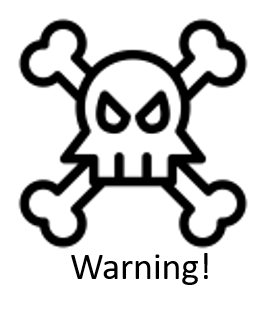
\includegraphics[width=0.077\textwidth,valign=m]{warning.png}
	   \colorbox{Gray!50}{\usebox{\graybox}}\hfill
	   \end{minipage}
	   \par\addvspace{\baselineskip}
	 }

%bestpractices enviroment	   
\newenvironment{bestpractices}
	{ \par\addvspace{\baselineskip}
	  \centering
	  \begin{minipage}{\textwidth} 
	  \begin{lrbox}{\graybox} 
	  \begin{varwidth}{0.9\textwidth}
	 }
	 {\end{varwidth}
	   \end{lrbox}
	   
\includegraphics[width=0.077\textwidth,valign=m]{bestpractices.png}
	   \colorbox{Gray!50}{\usebox{\graybox}}\hfill
	   \end{minipage}
	   \par\addvspace{\baselineskip}
	 }
	  
%complement enviroment
\newlength{\currentparindent}
\newenvironment{complement}[1]
      { \par\addvspace{\baselineskip}
        \setlength{\currentparindent}{\parindent}
        \centering
        \begin{lrbox}{\graybox}
        \begin{minipage}{\textwidth}
        \textbf{#1}
       	\setlength{\parindent}{\currentparindent}
       	{\color{Black}   \vspace{0.5ex} \hrule height 0.1ex} \vspace{0.5ex}}
      {
        \end{minipage}
        \end{lrbox}
        \colorbox{Gray!50}{\usebox{\graybox}}
        \par\addvspace{\baselineskip}
       }  

\usepackage{changepage}
\newenvironment{codeout}
{\par\addvspace{0.5\baselineskip}
\begin{adjustwidth}{\parindent}{0em}
\begin{minipage}{\linewidth}
\bfseries\small
}
{\end{minipage}
\end{adjustwidth}
\addvspace{0.5\baselineskip}
}
	
       
%type­sets text in mul­ti­ple columns (up to a max­i­mum of 10)
\usepackage{multicol}
\setlength\columnsep{15pt}
%description environment
\usepackage{enumitem} 
\setenumerate{itemsep=0.1em}

%use \cmidrule \toprule
\usepackage{booktabs}

% minitoc is incompatible with titletoc, so make the part toc with package titletoc
% add mini-ta­bles-of-con­tents (mini­tocs) at the be­gin­ning of ev­ery chap­ter, part or sec­tion.
%\usepackage{minitoc}
%\setcounter{minitocdepth}{1} 
%\renewcommand\tightmtcfalse

%set two text form
\definecolor{Kblue}{rgb}{0.24,0.36,0.65}
\newcommand\known[1]{\textcolor{Blue}{\emph{#1}}}
\newcommand\vital[1]{\textcolor{Plum!30!Cyan}{\textbf{#1}}}

%exercise
\usepackage{xsim}
\usepackage[skins]{tcolorbox}
\xsimsetup{solution/print=false}
\DeclareExerciseEnvironmentTemplate{tcolorbox}{%
    \par\addvspace{0.5\baselineskip}
    \tcolorbox[enhanced,left=2pt,right=2pt,title=\large{\textbf{\GetExerciseName~\thesubsection}},
   colback=\thepagecolor,colframe=gray,colbacktitle=NavyBlue!50,coltitle=black]%
}{\endtcolorbox}
\DeclareExerciseType{exercises}{
    exercise-env=exercises,
    solution-env=solutions,
    exercise-name=Exercises Section,
    solution-name=Solutions Section,
    exercise-template=tcolorbox,
    solution-template=tcolorbox,
    within=chapter,
    the-counter={\arabic{exercises}},
}

\newcounter{question}[chapter]
\newenvironment{question}
  {\refstepcounter{question}\textbf{Exercise \thechapter.\thequestion :}}{}

%change page color for chapter summary and defined terms (\pagecolor \pagebreak \newpagecolor \afterpage)
\usepackage[pagecolor=OliveGreen!30]{pagecolor}
\usepackage{afterpage}

%define a new command named cdotfill
\makeatletter
\newcommand\cdotfill{%
    \leavevmode\cleaders\hb@xt@.44em{\hss$\cdot$\hss}\hfill\kern\z@
}
\makeatother

% to make a mini table by package titletoc instead of minitoc
%chaptercontents
\newcommand\startchaptercontents{
\vspace*{3pc}
\startcontents
\newpagecolor{OliveGreen!50}\afterpage{\restorepagecolor}%
{\normalsize\bfseries\contentsname\endgraf\vspace{5pt}}
\contentsmargin{1em}
\titlerule
\addvspace{0.3ex}
\printcontents{l}{1}{\setcounter{tocdepth}{1}}
\addvspace{0.2ex}
\titlerule
\addvspace{3ex}
}
%partcontents
\newcommand\startpartcontents{
\vspace*{3pc}
\startcontents[parts]
\newpagecolor{OliveGreen!70}\afterpage{\afterpage{\restorepagecolor}}%
{\noindent\normalsize\bfseries\contentsname\endgraf\vspace{5pt}}
\contentsmargin{1em}
\titlerule
\addvspace{0.3ex}
\printcontents[parts]{l}{0}{\setcounter{tocdepth}{0}}
\addvspace{0.2ex}
\titlerule
\addvspace{3ex}
}

% draw picture and color the cover
\usepackage{tikz}
\newlength\amount
\setlength{\amount}{0.33\paperheight}

%long table
\usepackage{longtable}

%\makecell command
\usepackage{makecell}

%\hhline command
\usepackage{hhline}

%\caption* command
\usepackage{caption}

%color tbular
\usepackage{colortbl}

\begin{document}
%initialize minitoc
%\dominitoc 

\frontmatter
\begin{tikzpicture}[remember picture,overlay]
  \fill[White] (current page.north west) rectangle ([yshift=-\amount]current page.north east);
  \fill[Gray!50] ([yshift=-\amount]current page.north west) rectangle ([yshift=-2\amount]current page.north east);
  \fill[White]([yshift=-2\amount]current page.north west) rectangle (current page.south east);
\end{tikzpicture}
{\let\newpage\relax\maketitle}

\chapter*{Preface}
\vfill
\epigraph{\textit{To myself, keep calm and carry on.}}{--- KSC}
\vfill
\tableofcontents
\chapter*{New features in C++11}
\begin{enumerate}[align=parleft,itemsep=-2ex]
\item[\ref{c++11:long long}] \verb|long long| Type \cdotfill \pageref{c++11:long long} \\
\item[\ref{c++11:list initialization}] List Initialization \cdotfill \pageref{c++11:list initialization} \\
\end{enumerate}

\mainmatter
\chapter{Getting Started}\label{chap:getting started}
\startchaptercontents
%\minitoc 
This chapter introduces most of the basic elements of C++: types, variables,
expressions, statements, and functions. Along the way, we’ll briefly explain how to
compile and execute a program.

After having read this chapter and worked through the exercises, you should be able
to write, compile, and execute simple programs. Later chapters will assume that you
can use the features introduced in this chapter, and will explain these features in more
detail.
\newpage
The way to learn a new programming language is to write programs. In this chapter,
we’ll write a program to solve a simple problem for a bookstore.

Our store keeps a file of transactions, each of which records the sale of one or
more copies of a single book. Each transaction contains three data elements:
\begin{codeout}
 0-201-70353 \quad 4 \quad 24.99
\end{codeout}
The first element is an ISBN (International Standard Book Number, a unique book
identifier), the second is the number of copies sold, and the last is the price at which
each of these copies was sold. From time to time, the bookstore owner reads this file
and for each book computes the number of copies sold, the total revenue from that
book, and the average sales price.

To be able to write this program, we need to cover a few basic C++ features. In
addition, we’ll need to know how to compile and execute a program.

Although we haven’t yet designed our program, it’s easy to see that it must
\begin{itemize}
	\item Define variables
	\item Do input and output
	\item Use a data structure to hold the data
	\item Test whether two records have the same ISBN
	\item Contain a loop that will process every record in the transaction file
\end{itemize}
We’ll start by reviewing how to solve these subproblems in C++ and then write our
bookstore program.

	\section{Writing a Simple C++ Program}\label{sec:writing a simple c++ program}
	Every C++ program contains one or more \known{functions}, one of which must be named
\vital{main}. The operating system runs a C++ program by calling \verb|main|. Here is a simple
version of \verb|main| that does nothing but return a value to the operating system:
\begin{lstlisting}[label={lst:simple main}]
int main ()
{
   return 0 ;
}
\end{lstlisting}
	
	A function definition has four elements: a \known{return type}, a \known{function name}, a (possibly
empty) \known{parameter list} enclosed in parentheses, and a \known{function body}. Although \verb|main| is
special in some ways, we define \verb|main| the same way we define any other function.

In this example, \verb|main| has an empty list of parameters (shown by the \verb|()| with
nothing inside). \S~\ref{subsec:main handling cl opt} (p. \pageref{subsec:main handling cl opt}) will discuss the other parameter types that we can
define for \verb|main|.

The \verb|main| function is required to have a return type of \verb|int|, which is a type that
represents integers. The int type is a \vital{built-in type}, which means that it is one of
the types the language defines.

The final part of a function definition, the function body, is a \known{block} of \known{statements}
starting with an open \vital{curly brace} and ending with a close curly:
\begin{lstlisting}
{
   return 0 ;
}
\end{lstlisting}
The only statement in this block is a \verb|return|, which is a statement that terminates a
function. As is the case here, a \verb|return| can also send a value back to the function’s
caller. When a \verb|return| statement includes a value, the value returned must have a
type that is compatible with the return type of the function. In this case, the return
type of \verb|main| is \verb|int| and the return value is 0, which is an \verb|int|.
\begin{note}
		Note the semicolon at the end of the \verb|return| statement. Semicolons mark
the end of most statements in C++. They are easy to overlook but, when
forgotten, can lead to mysterious compiler error messages.
\end{note}

On most systems, the value returned from \verb|main| is a status indicator. A return value
of 0 indicates success. A nonzero return has a meaning that is defined by the system.Ordinarily a nonzero return indicates what kind of error occurred.
\begin{complement}{Key Concept: Types}
Types are one of the most fundamental concepts in programming and a
concept that we will come back to over and over in this Primer. A type
defines both the contents of a data element and the operations that are
possible on those data.
The data our programs manipulate are stored in variables and every
variable has a type. When the type of a variable named v is T, we often say
that “v has type T” or, interchangeably, that “v is a T.”
\end{complement}
		
		\subsection{Compiling and Executing Our Program}
Having written the program, we need to compile it. How you compile a program
depends on your operating system and compiler. For details on how your particular
compiler works, check the reference manual or ask a knowledgeable colleague.

Many PC-based compilers are run from an integrated development environment
(IDE) that bundles the compiler with build and analysis tools. These environments can
be a great asset in developing large programs but require a fair bit of time to learn
how to use effectively. Learning how to use such environments is well beyond the
scope of this book.

Most compilers, including those that come with an IDE, provide a command-line
interface. Unless you already know the IDE, you may find it easier to start with the
command-line interface. Doing so will let you concentrate on learning C++ first.
Moreover, once you understand the language, the IDE is likely to be easier to learn.
			\paragraph{Program Source File Naming Convention}
Whether you use a command-line interface or an IDE, most compilers expect program
source code to be stored in one or more files. Program files are normally referred to
as a \known{source files}. On most systems, the name of a source file ends with a suffix,
which is a period followed by one or more characters. The suffix tells the system that
the file is a C++ program. Different compilers use different suffix conventions; the
most common include .cc, .cxx, .cpp, .cp, and .C.
			\paragraph{Running the Compiler from the Command Line}
If we are using a command-line interface, we will typically compile a program in a
console window (such as a shell window on a UNIX system or a Command Prompt
window on Windows). Assuming that our main program is in a file named prog1.cc,
we might compile it by using a command such as
\begin{codeout}
\$ CC prog1.cc
\end{codeout}
where CC names the compiler and \$ is the system prompt. The compiler generates an
executable file. On a Windows system, that executable file is named prog1.exe.
UNIX compilers tend to put their executables in files named a.out.

To run an executable on Windows, we supply the executable file name and can omit
the .exe file extension:
\begin{codeout}
\$ prog1
\end{codeout}

On some systems you must specify the file’s location explicitly, even if the file is in the
current directory or folder. In such cases, we would write
\begin{codeout}
\$ .\textbackslash prog1
\end{codeout}
The “.” followed by a backslash indicates that the file is in the current directory.

To run an executable on UNIX, we use the full file name, including the file
extension:
\begin{codeout}
\$ ./a.out
\end{codeout}

The value returned from main is accessed in a system-dependent manner. On both
UNIX and Windows systems, after executing the program, you must issue an
appropriate echo command.

On UNIX systems, we obtain the status by writing
\begin{codeout}
\$ echo \$ ?
\end{codeout}
To see the status on a Windows system, we write
\begin{codeout}
\$ echo \%ERRORLEVEL\%
\end{codeout}
\begin{complement}{Running the GNU or Microsoft Compilers}
The command used to run the C++ compiler varies across compilers and
operating systems. The most common compilers are the GNU compiler and
the Microsoft Visual Studio compilers. By default, the command to run the
GNU compiler is g++:

\verb|$ g++ -o prog1 prog1.cc|\\
Here \$ is the system prompt. The -o prog1 is an argument to the compiler
and names the file in which to put the executable file. This command
generates an executable file named prog1 or prog1.exe, depending on the
operating system. On UNIX, executable files have no suffix; on Windows, the
suffix is .exe. If the -o prog1 is omitted, the compiler generates an
executable named a.out on UNIX systems and a.exe on Windows. (Note:
Depending on the release of the GNU compiler you are using, you may need
to specify -std=c++0x to turn on C++ 11 support.)

The command to run the Microsoft Visual Studio 2010 compiler is cl:

\verb|C:\Users\me\Programs> cl /EHsc prog1.cpp|\\
Here \verb|C:\Users\me\Programs>| is the system prompt and
\verb|\Users\me\Programs| is the name of the current directory (aka the current
folder). The cl command invokes the compiler, and /EHsc is the compiler
option that turns on standard exception handling. The Microsoft compiler
automatically generates an executable with a name that corresponds to the
first source file name. The executable has the suffix .exe and the same
name as the source file name. In this case, the executable is named
prog1.exe.

Compilers usually include options to generate warnings about problematic
constructs. It is usually a good idea to use these options. Our preference is
to use -Wall with the GNU compiler, and to use /W4 with the Microsoft
compilers.


For further information consult your compiler’s user’s guide.
\end{complement}
\begin{exercises}
\begin{question}
Review the documentation for your compiler and determine
what file naming convention it uses. Compile and run the \verb|main| program from
page \pageref{lst:simple main}.
\end{question}
            	
\begin{question}
Change the program to return -1. A return value of -1 is
often treated as an indicator that the program failed. Recompile and rerun
your program to see how your system treats a failure indicator from \verb|main|.
\end{question}
\end{exercises}

	\section{A First Look at Input/Output}\label{sec:a first look at input/output}
The C++ language does not define any statements to do input or output (IO).
Instead, C++ includes an extensive \vital{standard library} that provides IO (and many
other facilities). For many purposes, including the examples in this book, one needs to
know only a few basic concepts and operations from the IO library.

Most of the examples in this book use the \vital{iostream} library. Fundamental to the
\verb|iostream| library are two types named \vital{istream} and \vital{ostream}, which represent input
and output streams, respectively. A stream is a sequence of characters read from or
written to an IO device. The term stream is intended to suggest that the characters
are generated, or consumed, sequentially over time.
			\paragraph{Standard Input and Output Objects}
The library defines four IO objects. To handle input, we use an object of type
\verb|istream| named \vital{cin} (pronounced see-in). This object is also referred to as the
\vital{standard input}. For output, we use an ostream object named cout (pronounced
see-out). This object is also known as the \vital{standard output}. The library also defines
two other \verb|ostream| objects, named \vital{cerr} and \vital{clog} (pronounced see-err and see-log,
respectively). We typically use \verb|cerr|, referred to as the \vital{standard error}, for warning
and error messages and \verb|clog| for general information about the execution of the
program.
Ordinarily, the system associates each of these objects with the window in which
the program is executed. So, when we read from \verb|cin|, data are read from the window
in which the program is executing, and when we write to \verb|cout|, \verb|cerr|, or \verb|clog|, the
output is written to the same window.
			\paragraph{A Program That Uses the IO Library}
In our bookstore problem, we’ll have several records that we’ll want to combine into a
single total. As a simpler, related problem, let’s look first at how we might add two
numbers. Using the IO library, we can extend our main program to prompt the user
to give us two numbers and then print their sum:
\begin{lstlisting}[label={lst:read two number and print sum}]
#include <iostream>
int main()
{
   std::cout << "Enter two numbers:" << std::endl;
   int v1 = 0, v2 = 0;
   std::cin >> v1 >> v2;
   std::cout << "The sum of " << v1 << " and " << v2
           << " is " << v1 + v2 << std::endl;
   return 0;
}
\end{lstlisting}
This program starts by printing
\begin{codeout}
Enter two numbers:
\end{codeout}
on the user’s screen and then waits for input from the user. If the user enters
followed by a newline, then the program produces the following output:
\begin{codeout}
The sum of 3 and 7 is 10
\end{codeout}
The first line of our program
\begin{lstlisting}
#include <iostream>
\end{lstlisting}
tells the compiler that we want to use the \verb|iostream| library. The name inside angle
brackets (\verb|iostream| in this case) refers to a \vital{header}. Every program that uses a
library facility must include its associated header. The \verb|#include| directive must be
written on a single line—the name of the header and the \verb|#include| must appear on
the same line. In general, \verb|#include| directives must appear outside any function.
Typically, we put all the \verb|#include| directives for a program at the beginning of the
source file.
			\paragraph{Writing to a Stream}
The first statement in the body of \verb|main| executes an \vital{expression}. In C++ an
expression yields a result and is composed of one or more operands and (usually) an
operator. The expressions in this statement use the output operator (the \verb|«| operator)
to print a message on the standard output:
\begin{lstlisting}
std::cout << "Enter two numbers:" << std::endl;
\end{lstlisting}
The \verb|<<| operator takes two operands: The left-hand operand must be an \verb|ostream|
object; the right-hand operand is a value to print. The operator writes the given value
on the given \verb|ostream|. The result of the output operator is its left-hand operand.
That is, the result is the \verb|ostream| on which we wrote the given value.

Our output statement uses the \verb|<<| operator twice. Because the operator returns its
left-hand operand, the result of the first operator becomes the left-hand operand of
the second. As a result, we can chain together output requests. Thus, our expression
is equivalent to
\begin{lstlisting}
(std::cout << "Enter two numbers:") << std::endl;
\end{lstlisting}
Each operator in the chain has the same object as its left-hand operand, in this case
\verb|std::cout|. Alternatively, we can generate the same output using two statements:
\begin{lstlisting}
std::cout << "Enter two numbers:";
std::cout << std::endl;
\end{lstlisting}
The first output operator prints a message to the user. That message is a \vital{string literal}, 
which is a sequence of characters enclosed in double quotation marks. The
text between the quotation marks is printed to the standard output.

The second operator prints \verb|endl|, which is a special value called a \vital{manipulator}.\label{txt:endl manipulator}
Writing \verb|endl| has the effect of ending the current line and flushing the \known{buffer}
associated with that device. Flushing the buffer ensures that all the output the
program has generated so far is actually written to the output stream, rather than
sitting in memory waiting to be written.	
\begin{warning}
Programmers often add print statements during debugging. Such statements
should always flush the stream. Otherwise, if the program crashes, output
may be left in the buffer, leading to incorrect inferences about where the
program crashed.	
\end{warning}
			\paragraph{Using Names from the Standard Library}\label{par:using names from the standard library}
Careful readers will note that this program uses \verb|std::cout| and \verb|std::endl| rather
than just \verb|cout| and \verb|endl|. The prefix \verb|std::| indicates that the names \verb|cout| and \verb|endl|
are defined inside the \vital{namespace} named \vital{std}. Namespaces allow us to avoid
inadvertent collisions between the names we define and uses of those same names
inside a library. All the names defined by the standard library are in the \verb|std|
namespace.

One side effect of the library’s use of a namespace is that when we use a name
from the library, we must say explicitly that we want to use the name from the std
namespace. Writing \verb|std::cout| uses the scope operator (the \vital{:: operator}) \label{txt:scope operator} to say
that we want to use the name \verb|cout| that is defined in the namespace \verb|std|. \S~ \ref{sec:namespace using declarations} (p.
\pageref{sec:namespace using declarations}) will show a simpler way to access names from the library.
			\paragraph{Reading from a Stream}
Having asked the user for input, we next want to read that input. We start by defining
two \known{variables} named \verb|v1| and \verb|v2| to hold the input:
\begin{lstlisting}
int v1 = 0, v2 = 0;
\end{lstlisting}
We define these variables as type \verb|int|, which is a built-in type representing integers.
We also \known{initialize} them to 0. When we initialize a variable, we give it the indicated
value at the same time as the variable is created.

The next statement
\begin{lstlisting}
std::cin >> v1 >> v2;
\end{lstlisting}
reads the input. The input operator (the \verb|»| operator) behaves analogously to the
output operator. It takes an \verb|istream| as its left-hand operand and an object as its
right-hand operand. It reads data from the given \verb|istream| and stores what was read
in the given object. Like the output operator, the input operator returns its left-hand
operand as its result. Hence, this expression is equivalent to
\begin{lstlisting}
(std::cin >> v1) >> v2;
\end{lstlisting}
Because the operator returns its left-hand operand, we can combine a sequence of
input requests into a single statement. Our input operation reads two values from
\verb|std::cin|, storing the first in \verb|v1| and the second in \verb|v2|. In other words, our input
operation executes as
\begin{lstlisting}
std::cin >> v1;
std::cin >> v2;
\end{lstlisting}
			\paragraph{Completing the Program}
What remains is to print our result:
\begin{lstlisting}
std::cout << "The sum of " << v1 << " and " << v2
        << " is " << v1 + v2 << std::endl;
\end{lstlisting}
This statement, although longer than the one that prompted the user for input, is
conceptually similar. It prints each of its operands on the standard output. What is
interesting in this example is that the operands are not all the same kinds of values.
Some operands are string literals, such as \verb|"The sum of "|. Others are \verb|int| values,
such as \verb|v1|, \verb|v2|, and the result of evaluating the arithmetic expression \verb|v1 + v2|. The
library defines versions of the input and output operators that handle operands of
each of these differing types.
\begin{exercises}
\begin{question}
Write a program to print \verb|Hello, World| on the standard
output.
\end{question}
		
\begin{question}
Our program used the addition operator, \verb|+|, to add two
numbers. Write a program that uses the multiplication operator, \verb|*|, to print
the product instead.
\end{question}
		
\begin{question}
We wrote the output in one large statement. Rewrite the
program to use a separate statement to print each operand.
\end{question}
		
\begin{question}
Explain whether the following program fragment is legal.
\begin{lstlisting}
std::cout << "The sum of " << v1;
        << " and " << v2;
        << " is " << v1 + v2 << std::endl;
\end{lstlisting}	
If the program is legal, what does it do? If the program is not legal, why
not? How would you fix it?
\end{question}
\end{exercises}
	
	\section{A Word about Comments}
Before our programs get much more complicated, we should see how C++ handles
\known{comments}. Comments help the human readers of our programs. They are typically
used to summarize an algorithm, identify the purpose of a variable, or clarify an
otherwise obscure segment of code. The compiler ignores comments, so they have no
effect on the program’s behavior or performance.

Although the compiler ignores comments, readers of our code do not. Programmers
tend to believe comments even when other parts of the system documentation are out
of date. An incorrect comment is worse than no comment at all because it may
mislead the reader. When you change your code, be sure to update the comments,
too!
			\paragraph{Kinds of Comments in C++}
There are two kinds of comments in C++: single-line and paired. A single-line
comment starts with a double slash (\verb|//|) and ends with a newline. Everything to the
right of the slashes on the current line is ignored by the compiler. A comment of this
kind can contain any text, including additional double slashes.

The other kind of comment uses two delimiters (\verb|/*| and \verb|*/|) that are inherited from
C. Such comments begin with a \verb|/*| and end with the next \verb|*/|. These comments can
include anything that is not a \verb|*/|, including newlines. The compiler treats everything
that falls between the \verb|/*| and \verb|*/| as part of the comment.

A comment pair can be placed anywhere a tab, space, or newline is permitted.
Comment pairs can span multiple lines of a program but are not required to do so.
When a comment pair does span multiple lines, it is often a good idea to indicate
visually that the inner lines are part of a multiline comment. Our style is to begin each
line in the comment with an asterisk, thus indicating that the entire range is part of a
multiline comment.

Programs typically contain a mixture of both comment forms. Comment pairs
generally are used for multiline explanations, whereas double-slash comments tend to
be used for half-line and single-line remarks:
\begin{lstlisting}
#include <iostream>
/*
* Simple main function:
* Read two numbers and write their sum
*/
int main()
{
   // prompt user to enter two numbers
   std::cout << "Enter two numbers:" << std::endl;
   int v1 = 0, v2 = 0; // variables to hold the input we read
   std::cin >> v1 >> v2; // read input
   std::cout << "The sum of " << v1 << " and " << v2
   << " is " << v1 + v2 << std::endl;
   return 0;
}
\end{lstlisting}

\begin{note}
In this book, we italicize comments to make them stand out from the normal
program text. In actual programs, whether comment text is distinguished
from the text used for program code depends on the sophistication of the
programming environment you are using.
\end{note}
			\paragraph{Comment Pairs Do Not Nest}
A comment that begins with /* ends with the next */. As a result, one comment pair
cannot appear inside another. The compiler error messages that result from this kind
of mistake can be mysterious and confusing. As an example, compile the following
program on your system:
\begin{lstlisting}
/*
* comment pairs /* */ cannot nest.
* ''cannot nest'' is considered source code,
* as is the rest of the program
*/
int main()
{
   return 0;
}
\end{lstlisting}

We often need to comment out a block of code during debugging. Because that
code might contain nested comment pairs, the best way to comment a block of code
is to insert single-line comments at the beginning of each line in the section we want
to ignore:
\begin{lstlisting}
// /*
// * everything inside a single-line comment is ignored
// * including nested comment pairs
// */
\end{lstlisting}

\begin{exercises}
\begin{question}
Compile a program that has incorrectly nested comments.
\end{question}

\begin{question}
Indicate which, if any, of the following output statements are
legal:
\begin{verbatim}
std::cout << "/*";
std::cout << "*/";
std::cout << /* "*/" */;
std::cout << /* "*/" /* "/*" */;
\end{verbatim}
After you’ve predicted what will happen, test your answers by compiling a
program with each of these statements. Correct any errors you encounter.
\end{question}
\end{exercises}

	\section{Flow of Control}
Statements normally execute sequentially: The first statement in a block is executed
first, followed by the second, and so on. Of course, few programs—including the one
to solve our bookstore problem—can be written using only sequential execution.
Instead, programming languages provide various flow-of-control statements that allow
for more complicated execution paths.
		\subsection{The while Statement}\label{subsec:the while statement}
A \vital{while statement} repeatedly executes a section of code so long as a given condition
is true. We can use a \verb|while| to write a program to sum the numbers from 1 through
10 inclusive as follows:
\begin{lstlisting}
#include <iostream>
int main()
{
   int sum = 0, val = 1;
   // keep executing the while as long as val is less than or equal to 10
   while (val <= 10) {
      sum += val; // assigns sum + val to sum
      ++val; // add 1 to val
   }
   std::cout << "Sum of 1 to 10 inclusive is "
           << sum << std::endl;
   return 0;
}
\end{lstlisting}
When we compile and execute this program, it prints
\begin{codeout}
Sum of 1 to 10 inclusive is 55
\end{codeout}

As before, we start by including the \verb|iostream| header and defining \verb|main|. Inside
\verb|main| we define two \verb|int| variables: \verb|sum|, which will hold our summation, and \verb|val|,
which will represent each of the values from 1 through 10. We give sum an initial
value of \verb|0| and start \verb|val| off with the value \verb|1|.

The new part of this program is the \verb|while| statement. A \verb|while| has the form
\begin{lstlisting}
while (condition)
   statement
\end{lstlisting}
A \verb|while| executes by (alternately) testing the condition and executing the associated
statement until the condition is false. A \vital{condition} is an expression that yields a result
that is either true or false. So long as condition is true, statement is executed. After
executing statement, condition is tested again. If condition is again true, then
statement is again executed. The \verb|while| continues, alternately testing the condition
and executing statement until the condition is false.

In this program, the \verb|while| statement is
\begin{lstlisting}[label={lst:while statement}]
// keep executing the while as long as val is less than or equal to 10
while (val <= 10) {
   sum += val; // assigns sum + val to sum
   ++val; // add 1 to val
}
\end{lstlisting}
The condition uses the less-than-or-equal operator (the \vital{<= operator}) to compare the
current value of \verb|val| and 10. As long as \verb|val| is less than or equal to 10, the condition
is true. If the condition is true, we execute the body of the \verb|while|. In this case, that
body is a block with two statements:
\begin{lstlisting}
{
   sum += val; // assigns sum + val to sum
   ++val; // add 1 to val
}
\end{lstlisting}
A block is a sequence of zero or more statements enclosed by curly braces. A block is
a statement and may be used wherever a statement is required. The first statement in
this block uses the compound assignment operator (the += operator). This operator
adds its right-hand operand to its left-hand operand and stores the result in the lefthand
operand. It has essentially the same effect as writing an addition and an \vital{assignment}:
\begin{lstlisting}
sum = sum + val; // assign sum + val to sum
\end{lstlisting}
Thus, the first statement in the block adds the value of \verb|val| to the current value of
\verb|sum| and stores the result back into \verb|sum|.

The next statement
\begin{lstlisting}
++val; // add 1 to val
\end{lstlisting}
uses the prefix increment operator (the \vital{++ operator}). The increment operator adds \verb|1|
to its operand. Writing \verb|++val| is the same as writing \verb|val = val + 1|.

After executing the \verb|while| body, the loop evaluates the condition again. If the (now
incremented) value of \verb|val| is still less than or equal to 10, then the body of the
\verb|while| is executed again. The loop continues, testing the condition and executing the
body, until \verb|val| is no longer less than or equal to 10.

Once \verb|val| is greater than 10, the program falls out of the \verb|while| loop and continues
execution with the statement following the \verb|while|. In this case, that statement prints
our output, followed by the \verb|return|, which completes our \verb|main| program.
\begin{exercises}
\begin{question}
Write a program that uses a \verb|while| to sum the numbers from
50 to 100.
\end{question}

\begin{question}
In addition to the \verb|++| operator that adds 1 to its operand,
there is a decrement operator (\verb|--|) that subtracts 1. Use the decrement
operator to write a \verb|while| that prints the numbers from ten down to zero.
\end{question}

\begin{question}
Write a program that prompts the user for two integers.
Print each number in the range specified by those two integers.
\end{question}
\end{exercises}

		\subsection{The for Statement}\label{subsec:the for statement}
In our \verb|while| loop we used the variable \verb|val| to control how many times we executed
the loop. We tested the value of \verb|val| in the condition and incremented \verb|val| in the
\verb|while| body.

This pattern—using a variable in a condition and incrementing that variable in the
body—happens so often that the language defines a second statement, the \vital{for statement}, 
that abbreviates code that follows this pattern. We can rewrite this
program using a \verb|for| loop to sum the numbers from 1 through 10 as follows:
\begin{lstlisting}[label={lst:for statement}]
#include <iostream>
int main()
{
   int sum = 0;
   // sum values from 1 through 10 inclusive
   for (int val = 1; val <= 10; ++val)
      sum += val; // equivalent to sum = sum + val
   std::cout << "Sum of 1 to 10 inclusive is "
          << sum << std::endl;
   return 0;
}
\end{lstlisting}
As before, we define \verb|sum| and initialize it to zero. In this version, we define \verb|val| as
part of the \verb|for| statement itself:
\begin{lstlisting}
for (int val = 1; val <= 10; ++val)
   sum += val;
\end{lstlisting}
Each \verb|for| statement has two parts: a header and a body. The header controls how
often the body is executed. The header itself consists of three parts: an initstatement,
a condition, and an expression. In this case, the init-statement
\begin{lstlisting}
int val = 1;
\end{lstlisting}
defines an \verb|int| object named \verb|val| and gives it an initial value of 1. The variable \verb|val|
exists only inside the \verb|for|; it is not possible to use \verb|val| after this loop terminates. The
init-statement is executed only once, on entry to the \verb|for|. The condition
\begin{lstlisting}
val <= 10
\end{lstlisting}
compares the current value in \verb|val| to 10. The condition is tested each time through
the loop. As long as \verb|val| is less than or equal to 10, we execute the \verb|for| body. The
expression is executed after the \verb|for| body. Here, the expression
\begin{lstlisting}
++val
\end{lstlisting}
uses the prefix increment operator, which adds 1 to the value of \verb|val|. After executing
the expression, the \verb|for| retests the condition. If the new value of \verb|val| is still less than
or equal to 10, then the \verb|for| loop body is executed again. After executing the body,
\verb|val| is incremented again. The loop continues until the condition fails.

In this loop, the \verb|for| body performs the summation
\begin{lstlisting}
sum += val; // equivalent to sum = sum + val
\end{lstlisting}
To recap, the overall execution flow of this \verb|for| is:
\begin{enumerate}
	\item Create \verb|val| and initialize it to 1.
	\item Test whether \verb|val| is less than or equal to 10. If the test succeeds, execute the
\verb|for| body. If the test fails, exit the loop and continue execution with the first statement following the \verb|for| body.
	\item Increment \verb|val|.
	\item Repeat the test in step 2, continuing with the remaining steps as long as the
condition is true.
\end{enumerate}

\begin{exercises}
\begin{question}
What does the following \verb|for| loop do? What is the final value
of sum?
\begin{lstlisting}	
int sum = 0;
for (int i = -100; i <= 100; ++i)
   sum += i;
\end{lstlisting}
\end{question}

\begin{question}
Rewrite the exercises from \S~\ref{subsec:the while statement}(p. \pageref{subsec:the while statement}) using for loops.
\end{question}

\begin{question}
Compare and contrast the loops that used a \verb|for| with those
using a \verb|while|. Are there advantages or disadvantages to using either form?
\end{question}

\begin{question}
Write programs that contain the common errors discussed in
the box on page \pageref{box:compilation revisited}. Familiarize yourself with the messages the compiler
generates.
\end{question}
\end{exercises}

		\subsection{Reading an Unknown Number of Inputs}\label{subsec:reading an unknown number of inputs}
In the preceding sections, we wrote programs that summed the numbers from 1
through 10. A logical extension of this program would be to ask the user to input a set
of numbers to sum. In this case, we won’t know how many numbers to add. Instead,
we’ll keep reading numbers until there are no more numbers to read:
\begin{lstlisting}
#include <iostream>
int main()
{
   int sum = 0, value = 0;
   // read until end-of-file, calculating a running total of all values read
   while (std::cin >> value)
   sum += value; // equivalent to sum = sum + value
   std::cout << "Sum is: " << sum << std::endl;
   return 0;
}
\end{lstlisting}
If we give this program the input
\begin{codeout}
3 4 5 6
\end{codeout}
then our output will be
\begin{codeout}
Sum is: 18
\end{codeout}

The first line inside \verb|main| defines two \verb|int| variables, named \verb|sum| and \verb|value|, which
we initialize to 0. We’ll use \verb|value| to hold each number as we read it from the input.
We read the data inside the condition of the \verb|while|:
\begin{lstlisting}
while (std::cin >> value)
\end{lstlisting}
Evaluating the \verb|while| condition executes the expression
\begin{lstlisting}
std::cin >> value
\end{lstlisting}
That expression reads the next number from the standard input and stores that
number in \verb|value|. The input operator (\S~\ref{sec:a first look at input/output}, p. \pageref{sec:a first look at input/output} returns its left operand, which in
this case is \verb|std::cin|. This condition, therefore, tests \verb|std::cin|.

When we use an \verb|istream| as a condition, the effect is to test the state of the
stream. If the stream is valid—that is, if the stream hasn’t encountered an error—then
the test succeeds. An \verb|istream| becomes invalid when we hit \known{end-of-file} or encounter
an invalid input, such as reading a value that is not an integer. An \verb|istream| that is in
an invalid state will cause the condition to yield false.

Thus, our \verb|while| executes until we encounter end-of-file (or an input error). The
\verb|while| body uses the compound assignment operator to add the current value to the
evolving sum. Once the condition fails, the \verb|while| ends. We fall through and execute
the next statement, which prints the \verb|sum| followed by \verb|endl|.
\begin{complement}{Entering an End-of-File from the Keyboard}
When we enter input to a program from the keyboard, different operating
systems use different conventions to allow us to indicate end-of-file. On
Windows systems we enter an end-of-file by typing a control-z—hold down
the Ctrl key and press z—followed by hitting either the Enter or Return key.
On UNIX systems, including on Mac OS X machines, end-of-file is usually
control-d.
\end{complement}

\begin{complement}{Compilation Revisited}\label{box:compilation revisited}
Part of the compiler’s job is to look for errors in the program text. A compiler
cannot detect whether a program does what its author intends, but it can
detect errors in the form of the program. The following are the most common
kinds of errors a compiler will detect.
Syntax errors: The programmer has made a grammatical error in the C++
language. The following program illustrates common syntax errors; each
comment describes the error on the following line:
\begin{lstlisting}
// error: missing ) in parameter list for main
int main ( {
   // error: used colon, not a semicolon, after endl
   std::cout << "Read each file." << std::endl:
   // error: missing quotes around string literal
   std::cout << Update master. << std::endl;
   // error: second output operator is missing
   std::cout << "Write new master." std::endl;
   // error: missing ; on return statement
   return 0
}
\end{lstlisting}
Type errors: Each item of data in C++ has an associated type. The value 10,
for example, has a type of \verb|int| (or, more colloquially, “is an \verb|int|”). The word
\verb|"hello"|, including the double quotation marks, is a string literal. One
example of a type error is passing a string literal to a function that expects
an \verb|int| argument.\\
Declaration errors: Every name used in a C++ program must be declared
before it is used. Failure to declare a name usually results in an error
message. The two most common declaration errors are forgetting to use
\verb|std::| for a name from the library and misspelling the name of an identifier:
\begin{lstlisting}
#include <iostream>
int main()
{
   int v1 = 0, v2 = 0;
   std::cin >> v >> v2; // error: uses "v" not "v1"
   // error: cout not defined; should be std::cout
   cout << v1 + v2 << std::endl;
   return 0;
}
\end{lstlisting}

Error messages usually contain a line number and a brief description of
what the compiler believes we have done wrong. It is a good practice to
correct errors in the sequence they are reported. Often a single error can
have a cascading effect and cause a compiler to report more errors than
actually are present. It is also a good idea to recompile the code after each
fix—or after making at most a small number of obvious fixes. This cycle is
known as \known{edit-compile-debug}.
\end{complement}

\begin{exercises}
\begin{question}
Write your own version of a program that prints the sum of
a set of integers read from \verb|cin|.
\end{question}
\end{exercises}

		\subsection{The if Statement}
Like most languages, C++ provides an \vital{if statement} that supports conditional
execution. We can use an \verb|if| to write a program to count how many consecutive
times each distinct value appears in the input:
\begin{lstlisting}
#include <iostream>
int main()
{
   // currVal is the number we're counting; we'll read new values into val
   int currVal = 0, val = 0;
   // read first number and ensure that we have data to process
   if (std::cin >> currVal) {
      int cnt = 1; // store the count for the current value we're processing
      while (std::cin >> val) { // read the remaining numbers
         if (val == currVal) // if the values are the same
            ++cnt; // add 1 to cnt
         else { // otherwise, print the count for the previous value
	   std::cout << currVal << " occurs "
	           << cnt << " times" << std::endl;
	   currVal = val; // remember the new value
	   cnt = 1; // reset the counter
         }
      } // while loop ends here
      // remember to print the count for the last value in the file
      std::cout << currVal << " occurs "
              << cnt << " times" << std::endl;
} // outermost if statement ends here
   return 0;
}
\end{lstlisting}
If we give this program the following input:
\begin{codeout}
42 42 42 42 42 55 55 62 100 100 100
\end{codeout}
then the output should be
\begin{codeout}
42 occurs 5 times\\
55 occurs 2 times\\
62 occurs 1 times\\
100 occurs 3 times
\end{codeout}

Much of the code in this program should be familiar from our earlier programs. We
start by defining \verb|val| and \verb|currVal|: \verb|currVal| will keep track of which number we
are counting; \verb|val| will hold each number as we read it from the input. What’s new are
the two \verb|if| statements. The first \verb|if|
\begin{lstlisting}
if (std::cin >> currVal) {
   // ...
} // outermost if statement ends here
\end{lstlisting}
ensures that the input is not empty. Like a \verb|while|, an \verb|if| evaluates a condition. The
condition in the first \verb|if| reads a value into \verb|currVal|. If the read succeeds, then the
condition is true and we execute the block that starts with the open curly following the
condition. That block ends with the close curly just before the \verb|return| statement.

Once we know there are numbers to count, we define \verb|cnt|, which will count how
often each distinct number occurs. We use a \verb|while| loop similar to the one in the
previous section to (repeatedly) read numbers from the standard input.

The body of the \verb|while| is a block that contains the second \verb|if| statement:
\begin{lstlisting}
if (val == currVal) // if the values are the same
   ++cnt; // add 1 to cnt
else { // otherwise, print the count for the previous value
   std::cout << currVal << " occurs "
           << cnt << " times" << std::endl;
   currVal = val; // remember the new value
   cnt = 1; // reset the counter
}
\end{lstlisting}
The condition in this \verb|if| uses the equality operator (the \vital{== operator}) to test whether
\verb|val| is equal to \verb|currVa|l. If so, we execute the statement that immediately follows
the condition. That statement increments \verb|cnt|, indicating that we have seen \verb|currVal|
once more.

If the condition is false—that is, if \verb|val| is not equal to \verb|currVal|—then we execute
the statement following the \verb|else|. This statement is a block consisting of an output
statement and two assignments. The output statement prints the count for the value
we just finished processing. The assignments reset \verb|cnt| to 1 and \verb|currVal| to \verb|val|,
which is the number we just read.
\begin{warning}
C++ uses \verb|=| for assignment and \verb|==| for equality. Both operators can appear
inside a condition. It is a common mistake to write = when you mean \verb|==|
inside a condition.
\end{warning}

\begin{exercises}
\begin{question}
What happens in the program presented in this section if the
input values are all equal? What if there are no duplicated values?
\end{question}

\begin{question}
Compile and run the program from this section giving it only
equal values as input. Run it again giving it values in which no number is
repeated.
\end{question}

\begin{question}
Revise the program you wrote for the exercises in \S~\ref{subsec:the while statement} (p.
\pageref{subsec:the while statement}) that printed a range of numbers so that it handles input in which the first
number is smaller than the second.
\end{question}
\end{exercises}

\begin{complement}{Key Concept: Indentation and Formatting of C++ Programs}
C++ programs are largely free-format, meaning that where we put curly
braces, indentation, comments, and newlines usually has no effect on what
our programs mean. For example, the curly brace that denotes the beginning
of the body of \verb|main| could be on the same line as \verb|main|; positioned as we
have done, at the beginning of the next line; or placed anywhere else we’d
like. The only requirement is that the open curly must be the first nonblank,
noncomment character following \verb|main|’s parameter list.
Although we are largely free to format programs as we wish, the choices
we make affect the readability of our programs. We could, for example, have
written \verb|main| on a single long line. Such a definition, although legal, would be
hard to read.
Endless debates occur as to the right way to format C or C++ programs.
Our belief is that there is no single correct style but that there is value in
consistency. Most programmers indent subsidiary parts of their programs, as
we’ve done with the statements inside \verb|main| and the bodies of our loops. We
tend to put the curly braces that delimit functions on their own lines. We also
indent compound IO expressions so that the operators line up. Other
indentation conventions will become clear as our programs become more
sophisticated.
The important thing to keep in mind is that other ways to format programs
are possible. When you choose a formatting style, think about how it affects
readability and comprehension. Once you’ve chosen a style, use it
consistently.
\end{complement}

	\section{Introducing Classes}	\label{sec:introducing classes}
The only remaining feature we need to understand before solving our bookstore
problem is how to define a \known{data structure} to represent our transaction data. In C++
we define our own data structures by defining a \vital{class}. A class defines a type along
with a collection of operations that are related to that type. The class mechanism is
one of the most important features in C++. In fact, a primary focus of the design of
C++ is to make it possible to define \vital{class types} that behave as naturally as the built-in
types.

In this section, we’ll describe a simple class that we can use in writing our bookstore
program. We’ll implement this class in later chapters as we learn more about types,
expressions, statements, and functions.

To use a class we need to know three things:
\begin{itemize}
	\item What is its name?
	\item Where is it defined?
	\item What operations does it support?
\end{itemize}
For our bookstore problem, we’ll assume that the class is named \verb|Sales_item| and
that it is already defined in a header named \verb|Sales_item.h|.

As we’ve seen, to use a library facility, we must include the associated header.
Similarly, we use headers to access classes defined for our own applications.
Conventionally, header file names are derived from the name of a class defined in that
header. Header files that we write usually have a suffix of \verb|.h|, but some programmers
use \verb|.H|, \verb|.hpp|, or \verb|.hxx|. The standard library headers typically have no suffix at all.
Compilers usually don’t care about the form of header file names, but IDEs sometimes
do.

		\subsection{The Sales\_item Class}\label{subsec:the sales-item class}
The purpose of the \verb|Sales_item| class is to represent the total revenue, number of
copies sold, and average sales price for a book. How these data are stored or
computed is not our concern. To use a class, we need not care about how it is
implemented. Instead, what we need to know is what operations objects of that type
can perform.

Every class defines a type. The type name is the same as the name of the class.
Hence, our \verb|Sales_item| class defines a type named \verb|Sales_item|. As with the builtin
types, we can define a variable of a class type. When we write
\begin{lstlisting}
   Sales_item item;
\end{lstlisting}
we are saying that \verb|item| is an object of type \verb|Sales_item|. We often contract the
phrase “an object of type \verb|Sales_item|” to “a \verb|Sales_item| object” or even more
simply to “a \verb|Sales_item|.”

In addition to being able to define variables of type \verb|Sales_item|, we can:
\begin{itemize}
	\item Call a function named \verb|isbn| to fetch the from a \verb|Sales_item| object.
	\item Use the input (\verb|>>|) and output (\verb|<<|) operators to read and write objects of type
\verb|Sales_item|.
	\item Use the assignment operator (\verb|=|) to assign one \verb|Sales_item| object to another.
	\item Use the addition operator (\verb|+|) to add two \verb|Sales_item| objects. The two objects
must refer to the same ISBN. The result is a new \verb|Sales_item| object whose ISBN
is that of its operands and whose number sold and revenue are the sum of the
corresponding values in its operands.
	\item Use the compound assignment operator (\verb|+=|) to add one \verb|Sales_item| object
into another.
\end{itemize}

\begin{complement}{Key Concept: Classes Define Behavior}
The important thing to keep in mind when you read these programs is that
the author of the S\verb|ales_item| class defines all the actions that can be
performed by objects of this class. That is, the \verb|Sales_item| class defines
what happens when a \verb|Sales_item| object is created and what happens
when the assignment, addition, or the input and output operators are applied
to \verb|Sales_item|s.
In general, the class author determines all the operations that can be used
on objects of the class type. For now, the only operations we know we can
perform on \verb|Sales_item| objects are the ones listed in this section.
\end{complement}
			\paragraph{Reading and Writing Sales\_items}
Now that we know what operations we can use with \verb|Sales_item| objects, we can
write programs that use the class. For example, the following program reads data from
the standard input into a \verb|Sales_item| object and writes that \verb|Sales_item| back onto
the standard output:
\begin{lstlisting}
#include <iostream>
#include "Sales_item.h"
int main()
{
   Sales_item book;
   // read ISBN, number of copies sold, and sales price
   std::cin >> book;
   // write ISBN, number of copies sold, total revenue, and average price
   std::cout << book << std::endl;
   return 0;
}
\end{lstlisting}
If the input to this program is
\begin{codeout}
0-201-70353-X 4 24.99
\end{codeout}
then the output will be
\begin{codeout}
0-201-70353-X 4 99.96 24.99
\end{codeout}
Our input says that we sold four copies of the book at \$24.99 each, and the output
indicates that the total sold was four, the total revenue was \$99.96, and the average
price per book was \$24.99.

This program starts with two \verb|#include| directives, one of which uses a new form.
Headers from the standard library are enclosed in angle brackets (\verb|< >|). Those that
are not part of the library are enclosed in double quotes (\verb|" "|)

Inside \verb|main| we define an object, named \verb|book|, that we’ll use to hold the data that
we read from the standard input. The next statement reads into that object, and the
third statement prints it to the standard output followed by printing \verb|endl|.
			\paragraph{Adding Sales\_items}
\begin{lstlisting}
#include <iostream>
#include "Sales_item.h"
int main()
{
   Sales_item item1, item2;
   std::cin >> item1 >> item2; // read a pair of transactions
   std::cout << item1 + item2 << std::endl; // print their sum
   return 0;
}
\end{lstlisting}
If we give this program the following input
\begin{codeout}
0-201-78345-X 3 20.00\\
0-201-78345-X 2 25.00
\end{codeout}

our output is
\begin{codeout}
0-201-78345-X 5 110 22
\end{codeout}

This program starts by including the \verb|Sales_item| and \verb|iostream| headers. Next we
define two \verb|Sales_item| objects to hold the transactions. We read data into these
objects from the standard input. The output expression does the addition and prints
the result.

It’s worth noting how similar this program looks to the one on page \pageref{lst:read two number and print sum}: We read two
inputs and write their sum. What makes this similarity noteworthy is that instead of
reading and printing the sum of two integers, we’re reading and printing the sum of
two \verb|Sales_item| objects. Moreover, the whole idea of “sum” is different. In the case
of \verb|int|s we are generating a conventional sum—the result of adding two numeric
values. In the case of \verb|Sales_item| objects we use a conceptually new meaning for
sum—the result of adding the components of two \verb|Sales_item| objects.
\begin{complement}{Using File Redirection}
It can be tedious to repeatedly type these transactions as input to the
programs you are testing. Most operating systems support file redirection,
which lets us associate a named file with the standard input and the standard
output:
\begin{lstlisting}
$ addItems <infile >outfile
\end{lstlisting}
Assuming \verb|$| is the system prompt and our addition program has been
compiled into an executable file named \verb|addItems.exe| (or \verb|addItems| on
UNIX systems), this command will read transactions from a file named
\verb|infile| and write its output to a file named \verb|outfile| in the current
directory.
\end{complement}

\begin{exercises}
\begin{question}
\verb|http://www.informit.com/title/032174113| contains a copy of
\verb|Sales_item.h| in the Chapter 1 code directory. Copy that file to your
working directory. Use it to write a program that reads a set of book sales
transactions, writing each transaction to the standard output.
\end{question}

\begin{question}
Write a program that reads two \verb|Sales_item| objects that
have the same ISBN and produces their sum.
\end{question}

\begin{question}
Write a program that reads several transactions for the same
ISBN. Write the sum of all the transactions that were read.
\end{question}
\end{exercises}

		\subsection{A First Look at Member Functions}\label{subsec:a first look at member functions}
Our program that adds two \verb|Sales_item|s should check whether the objects have the
same ISBN. We’ll do so as follows:
\begin{lstlisting}[label={lst:add two objects of type sales-item}]
#include <iostream>
#include "Sales_item.h"
int main()
{
   Sales_item item1, item2;
   std::cin >> item1 >> item2;
   // first check that item1 and item2 represent the same book
   if (item1.isbn() == item2.isbn()) {
      std::cout << item1 + item2 << std::endl;
      return 0; // indicate success
   } 
   else {
      std::cerr << "Data must refer to same ISBN"
              << std::endl;
      return -1; // indicate failure
   }
}
\end{lstlisting}

The difference between this program and the previous version is the \verb|if| and its
associated \verb|else| branch. Even without understanding the \verb|if| condition, we know what
this program does. If the condition succeeds, then we write the same output as before
and return 0, indicating success. If the condition fails, we execute the block following
the \verb|else|, which prints a message and returns an error indicator.
			\paragraph{What Is a Member Function?}\label{par:what is a member function?}
The \verb|if| condition
\begin{lstlisting}
item1.isbn() == item2.isbn()
\end{lstlisting}
calls a \vital{member function} named \verb|isbn|. A member function is a function that is
defined as part of a class. Member functions are sometimes referred to as \vital{methods}.

Ordinarily, we call a member function on behalf of an object. For example, the first
part of the left-hand operand of the equality expression
\begin{lstlisting}
item1.isbn
\end{lstlisting}
uses the dot operator (the \vital{\texttt{"."} operator}) to say that we want “the \verb|isbn| member of
the object named \verb|item1|.” The dot operator applies only to objects of class type. The
left-hand operand must be an object of class type, and the right-hand operand must
name a member of that type. The result of the dot operator is the member named by
the right-hand operand.

When we use the dot operator to access a member function, we usually do so to
call that function. We call a function using the call operator (the \vital{() operator}). The call
operator is a pair of parentheses that enclose a (possibly empty) list of \known{arguments}.
The \verb|isbn| member function does not take an argument. Thus,
\begin{lstlisting}
item1.isbn()
\end{lstlisting}
calls the \verb|isbn| function that is a member of the object named \verb|item1|. This function
returns the ISBN stored in \verb|item1|.

The right-hand operand of the equality operator executes in the same way—it
returns the ISBN stored in \verb|item2|. If the ISBNs are the same, the condition is \verb|true|;
otherwise it is \verb|false|.
\begin{exercises}
\begin{question}
Write a program that reads several transactions and counts
how many transactions occur for each ISBN.
\end{question}

\begin{question}
Test the previous program by giving multiple transactions
representing multiple ISBNs. The records for each ISBN should be grouped
together.
\end{question}
\end{exercises}

	\section{The Bookstore Program}
We are now ready to solve our original bookstore problem. We need to read a file of
sales transactions and produce a report that shows, for each book, the total number
of copies sold, the total revenue, and the average sales price. We’ll assume that all
the transactions for each ISBN are grouped together in the input.

Our program will combine the data for each ISBN in a variable named \verb|total|. We’ll
use a second variable named \verb|trans| to hold each transaction we read. If \verb|trans| and
\verb|total| refer to the same ISBN, we’ll update \verb|total|. Otherwise we’ll print \verb|total| and
reset it using the transaction we just read:
\begin{lstlisting}[label={lst:the bookstore program}]
#include <iostream>
#include "Sales_item.h"
int main()
{
   Sales_item total; // variable to hold the running sum
   // read the first transaction and ensure that there are data to process
   if (std::cin >> total) {
      Sales_item trans; // variable to hold data for the next transaction
      // read and process the remaining transactions
      while (std::cin >> trans) {
         // if we're still processing the same book
         if (total.isbn() == trans.isbn())
            total += trans; // update the running total
         else {
            // print results for the previous book
	    std::cout << total << std::endl;
	    total = trans; // total now refers to the next book
         }
      }
      std::cout << total << std::endl; // print the last transaction
   } 
   else {
      // no input! warn the user
      std::cerr << "No data?!" << std::endl;
      return -1; // indicate failure
   }
   return 0;
}
\end{lstlisting}

This program is the most complicated one we’ve seen so far, but it uses only
facilities that we have already seen.

As usual, we begin by including the headers that we use, \verb|iostream| from the library
and our own \verb|Sales_item.h|. Inside \verb|main| we define an object named \verb|total|, which
we’ll use to sum the data for a given ISBN. We start by reading the first transaction
into \verb|total| and testing whether the read was successful. If the read fails, then there
are no records and we fall through to the outermost \verb|else| branch, which tells the user
that there was no input.

Assuming we have successfully read a record, we execute the block following the
outermost \verb|if|. That block starts by defining the object named \verb|trans|, which will hold
our transactions as we read them. The \verb|while| statement will read all the remaining
records. As in our earlier programs, the \verb|while| condition reads a value from the
standard input. In this case, we read a \verb|Sales_item| object into \verb|trans|. As long as
the read succeeds, we execute the body of the \verb|while|.

The body of the \verb|while| is a single \verb|if| statement. The \verb|if| checks whether the ISBNs
are equal. If so, we use the compound assignment operator to add \verb|trans| to \verb|total|.
If the ISBNs are not equal, we print the value stored in \verb|total| and reset \verb|total| by
assigning \verb|trans| to it. After executing the \verb|if|, we return to the condition in the
\verb|while|, reading the next transaction, and so on until we run out of records.

When the \verb|while| terminates, \verb|total| contains the data for the last ISBN in the file.
We write the data for the last ISBN in the last statement of the block that concludes
the outermost \verb|if| statement.
\begin{exercises}
\begin{question}\label{qst:compile and execute the bookstore program}
Using the \verb|Sales_item.h| header from the Web site,
compile and execute the bookstore program presented in this section.
\end{question}
\end{exercises}
	\newpage\newpagecolor{Goldenrod!20}
	\section*{Chapter Summary} \markright{Chapter Summary} \addcontentsline{toc}{section}{Chapter Summary}
This chapter introduced enough of C++ to let you compile and execute simple C++
programs. We saw how to define a \verb|main| function, which is the function that the
operating system calls to execute our program. We also saw how to define variables,
how to do input and output, and how to write \verb|if|, \verb|for|, and \verb|while| statements. The
chapter closed by introducing the most fundamental facility in C++: the class. In this
chapter, we saw how to create and use objects of a class that someone else has
defined. Later chapters will show how to define our own classes.
	\section*{Defined Terms} \markright{Defined Terms} \addcontentsline{toc}{section}{Defined Terms}
\begin{multicols}{2}
\begin{description}[leftmargin=0pt]
	\item[argument] Value passed to a function.
	\item[assignment] Obliterates an object’s current value and replaces that value by a
new one.
	\item[block] Sequence of zero or more statements enclosed in curly braces.
	\item[buffer] A region of storage used to hold data. IO facilities often store input (or
output) in a buffer and read or write the buffer independently from actions in the
program. Output buffers can be explicitly flushed to force the buffer to be written.
By default, reading \verb|cin| flushes \verb|cout|; \verb|cout| is also flushed when the program
ends normally.
	\item[built-in type] Type, such as \verb|int|, defined by the language.
	\item[cerr] \verb|ostream| object tied to the standard error, which often writes to the same
device as the standard output. By default, writes to \verb|cerr| are not buffered.
Usually used for error messages or other output that is not part of the normal
logic of the program.
	\item[character string literal] Another term for string literal.
	\item[cin] \verb|istream| object used to read from the standard input.
	\item[class] Facility for defining our own data structures together with associated
operations. The class is one of the most fundamental features in C++. Library
types, such as \verb|istream| and \verb|ostream|, are classes.
	\item[class type] A type defined by a class. The name of the type is the class name.
	\item[clog] \verb|ostream| object tied to the standard error. By default, writes to \verb|clog| are
buffered. Usually used to report information about program execution to a log file.
	\item[comment] Program text that is ignored by the compiler. C++ has two kinds of
comments: single-line and paired. Single-line comments start with a \verb|//|.
Everything from the \verb|//| to the end of the line is a comment. Paired comments
begin with a \verb|/*| and include all text up to the next \verb|*/|.
	\item[condition] An expression that is evaluated as true or false. A value of zero is
false; any other value yields true.
	\item[cout] \verb|ostream| object used to write to the standard output. Ordinarily used to
write the output of a program.
	\item[curly brace] Curly braces delimit blocks. An open curly (\verb|{|) starts a block; a close
curly (\verb|}|) ends one.
	\item[data structure] A logical grouping of data and operations on that data.
	\item[edit-compile-debug] The process of getting a program to execute properly.
	\item[end-of-file] System-specific marker that indicates that there is no more input in a
file.
	\item[expression] The smallest unit of computation. An expression consists of one or
more operands and usually one or more operators. Expressions are evaluated to
produce a result. For example, assuming \verb|i| and \verb|j| are \verb|int|s, then \verb|i + j| is an
expression and yields the sum of the two \verb|int| values.
	\item[for statement] Iteration statement that provides iterative execution. Often used
to repeat a calculation a fixed number of times.
	\item[function] Named unit of computation.
	\item[function body] Block that defines the actions performed by a function.
	\item[function name] Name by which a function is known and can be called.
	\item[header] Mechanism whereby the definitions of a class or other names are made
available to multiple programs. A program uses a header through a \verb|#include|
directive.
	\item[if statement] Conditional execution based on the value of a specified condition. If
the condition is true, the \verb|if| body is executed. If not, the \verb|else| body is executed
if there is one.
	\item[initialize] Give an object a value at the same time that it is created.
	\item[iostream] Header that provides the library types for stream-oriented input and
output.
	\item[istream] Library type providing stream-oriented input.
	\item[library type] Type, such as \verb|istream|, defined by the standard library.
	\item[main] Function called by the operating system to execute a C++ program. Each
program must have one and only one function named \verb|main|.
	\item[manipulator]Object, such as \verb|std::endl|, that when read or written
“manipulates” the stream itself.
	\item[member function] Operation defined by a class. Member functions ordinarily are
called to operate on a specific object.
	\item[method] Synonym for member function.
	\item[namespace] Mechanism for putting names defined by a library into a single
place. Namespaces help avoid inadvertent name clashes. The names defined by
the C++ library are in the namespace \verb|std|.
	\item[ostream] Library type providing stream-oriented output.
	\item[parameter list] Part of the definition of a function. Possibly empty list that
specifies what arguments can be used to call the function.
	\item[return type] Type of the value returned by a function.
	\item[source file] Term used to describe a file that contains a C++ program.
	\item[standard error] Output stream used for error reporting. Ordinarily, the standard
output and the standard error are tied to the window in which the program is
executed.
	\item[standard input] Input stream usually associated with the window in which the
program executes.
	\item[standard library] Collection of types and functions that every C++ compiler must
support. The library provides the types that support IO. C++ programmers tend
to talk about “the library,” meaning the entire standard library. They also tend to
refer to particular parts of the library by referring to a library type, such as the
“\verb|iostream| library,” meaning the part of the standard library that defines the IO
classes.
	\item[standard output] Output stream usually associated with the window in which the
program executes.
	\item[statement] A part of a program that specifies an action to take place when the
program is executed. An expression followed by a semicolon is a statement; other
kinds of statements include blocks and \verb|if|, \verb|for|, and \verb|while| statements, all of
which contain other statements within themselves.
	\item[std] Name of the namespace used by the standard library. \verb|std::cout| indicates
that we’re using the name \verb|cout| defined in the \verb|std| namespace.
	\item[string literal] Sequence of zero or more characters enclosed in double quotes
(\verb|"a string literal"|).
	\item[variable] A named object.
	\item[while statement] Iteration statement that provides iterative execution so long as
a specified condition is true. The body is executed zero or more times, depending
on the truth value of the condition.
	\item[() operator] Call operator. A pair of parentheses “\verb|()|” following a function name.
	The operator causes a function to be invoked. Arguments to the function may be
passed inside the parentheses.
	\item[\texttt{++} operator] Increment operator. Adds 1 to the operand; \verb|++i| is equivalent to \verb|i = i + 1|.
	\item[\texttt{+=} operator] Compound assignment operator that adds the right-hand operand to
the left and stores the result in the left-hand operand; \verb|a += b| is equivalent to \verb|a = a + b|.
	\item[\texttt{.} operator] Dot operator. Left-hand operand must be an object of class type and
the right-hand operand must be the name of a member of that object. The
operator yields the named member of the given object.
	\item[\texttt{::} operator] Scope operator. Among other uses, the scope operator is used to
access names in a namespace. For example, \verb|std::cout| denotes the name \verb|cout|
from the namespace \verb|std|.
	\item[\texttt{=} operator] Assigns the value of the right-hand operand to the object denoted by
the left-hand operand.
	\item[\texttt{--} operator] Decrement operator. Subtracts 1 from the operand; \verb|--i| is
equivalent to \verb|i = i - 1|.
	\item[\texttt{<<} operator] Output operator. Writes the right-hand operand to the output
stream indicated by the left-hand operand: \verb|cout << "hi"| writes hi to the
standard output. Output operations can be chained together: \verb|cout << "hi" << "bye"| writes \verb|hibye|.
	\item[\texttt{>>} operator] Input operator. Reads from the input stream specified by the lefthand
operand into the right-hand operand: \verb|cin >> i| reads the next value on
the standard input into \verb|i|. Input operations can be chained together: \verb|cin >> i >> j| 
reads first into i and then into \verb|j|.
	\item[\texttt{\#}include] Directive that makes code in a header available to a program.
	\item[\texttt{==} operator] The equality operator. Tests whether the left-hand operand is equal
to the right-hand operand.
	\item[\texttt{!=} operator] The inequality operator. Tests whether the left-hand operand is not
equal to the right-hand operand.
	\item[\texttt{<=} operator] The less-than-or-equal operator. Tests whether the left-hand
operand is less than or equal to the right-hand operand.
	\item[\texttt{<} operator] The less-than operator. Tests whether the left-hand operand is less
than the right-hand operand.
	\item[\texttt{>=} operator] Greater-than-or-equal operator. Tests whether the left-hand operand is greater than or equal to the right-hand operand.
	\item[\texttt{>} operator] Greater-than operator. Tests whether the left-hand operand is
greater than the right-hand operand.
\end{description}
\end{multicols}
\stopcontents
\pagebreak\restorepagecolor

\part{The Basics}
\startpartcontents
Every widely used programming language provides a common set of features, which
differ in detail from one language to another. Understanding the details of how a
language provides these features is the first step toward understanding the language.
Among the most fundamental of these common features are
\begin{itemize}
	\item Built-in types such as integers, characters, and so forth
	\item Variables, which let us give names to the objects we use
	\item Expressions and statements to manipulate values of these types
	\item Control structures, such as \verb|if| or \verb|while|, that allow us to conditionally or
repeatedly execute a set of actions
	\item Functions that let us define callable units of computation
\end{itemize}

Most programming languages supplement these basic features in two ways: They let
programmers extend the language by defining their own types, and they provide
library routines that define useful functions and types not otherwise built into the
language.

In C++, as in most programming languages, the type of an object determines what
operations can be performed on it. Whether a particular expression is legal depends
on the type of the objects in that expression. Some languages, such as Smalltalk and
Python, check types at run time. In contrast, C++ is a statically typed language; type
checking is done at compile time. As a consequence, the compiler must know the type
of every name used in the program.

C++ provides a set of built-in types, operators to manipulate those types, and a
small set of statements for program flow control. These elements form an alphabet
from which we can write large, complicated, real-world systems. At this basic level,
C++ is a simple language. Its expressive power arises from its support for
mechanisms that allow the programmer to define new data structures. Using these
facilities, programmers can shape the language to their own purposes without the
language designers having to anticipate the programmers’ needs.

Perhaps the most important feature in C++ is the class, which lets programmers
define their own types. In C++ such types are sometimes called “class types” to
distinguish them from the types that are built into the language. Some languages let
programmers define types that specify only what data make up the type. Others, like
C++, allow programmers to define types that include operations as well as data. A
major design goal of C++ is to let programmers define their own types that are as
easy to use as the built-in types. The Standard C++ library uses these features to
implement a rich library of class types and associated functions.

The first step in mastering C++—learning the basics of the language and library—is
the topic of Part I. Chapter 2 covers the built-in types and looks briefly at the
mechanisms for defining our own new types. Chapter 3 introduces two of the most
fundamental library types: \verb|string| and \verb|vector|. That chapter also covers arrays,
which are a lower-level data structure built into C++ and many other languages.
Chapters 4 through 6 cover expressions, statements, and functions. This part
concludes in Chapter 7, which describes the basics of building our own class types. As
we’ll see, defining our own types brings together all that we’ve learned before,
because writing a class entails using the facilities covered in Part I.

\chapter{Variables and Basic Types}\label{chap:variables and basic types}
%\minitoc 
\startchaptercontents
Types are fundamental to any program: They tell us what our data mean and what
operations we can perform on those data.

C++ has extensive support for types. The language defines several primitive types
(characters, integers, floating-point numbers, etc.) and provides mechanisms that let
us define our own data types. The library uses these mechanisms to define more
complicated types such as variable-length character strings, vectors, and so on. This
chapter covers the built-in types and begins our coverage of how C++ supports more
complicated types.
\newpage
Types determine the meaning of the data and operations in our programs. The
meaning of even as simple a statement as
\begin{lstlisting}
i = i + j;
\end{lstlisting}
depends on the types of \verb|i| and \verb|j|. If \verb|i| and \verb|j| are integers, this statement has the
ordinary, arithmetic meaning of \verb|+|. However, if \verb|i| and \verb|j| are \verb|Sales_item| objects (\S~
\ref{subsec:the sales-item class}, p. \pageref{subsec:the sales-item class}), this statement adds the components of these two objects.
	
	\section{Primitive Built-in Types}\label{sec:primitive built-in types}
C++ defines a set of primitive types that include the \vital{arithmetic types} and a special
type named \vital{void}. The arithmetic types represent characters, integers, boolean values,
and floating-point numbers. The \verb|void| type has no associated values and can be used
in only a few circumstances, most commonly as the return type for functions that do
not return a value.

		\subsection{Arithmetic Types}\label{subsec:arithmetic types}
The arithmetic types are divided into two categories: \vital{integral types} (which include
character and boolean types) and floating-point types.

The size of—that is, the number of bits in—the arithmetic types varies across
machines. The standard guarantees minimum sizes as listed in Table \ref{tab:arithmetic types}. However,
compilers are allowed to use larger sizes for these types. Because the number of bits
varies, the largest (or smallest) value that a type can represent also varies.
\begin{table}[H]
\caption{C++: Arithmetic Types}
\label{tab:arithmetic types}
\centering
\begin{tabular}{| lll |}
\hline
\textbf{Type} & \textbf{Meaning} & \textbf{Minimum Size} \\
\hline
\verb|bool| & boolean & NA \\
\verb|char| & character & 8bits \\
\verb|wchar_t| & wide character & 16bits \\
\verb|char16_t| & Unicode character & 16bits \\
\verb|char32_t| & Unicode character & 32bits \\
\verb|short| & short integer & 16bits \\
\verb|int| & integer & 16bits \\
\verb|long| & long integer & 32bits \\
\verb|long long| & long integer & 64bits \\
\verb|float| & single-precision floating-point & 6 significant digits \\
\verb|double| & double-precision floating-point & 10 significant digits \\
\verb|long double| & extended-precision floating-point & 10 significant digits \\
\hline
\end{tabular}
\end{table}

The \verb|bool| type represents the truth values \verb|true| and \verb|false|.

There are several character types, most of which exist to support
internationalization. The basic character type is \verb|char|. A \verb|char| is guaranteed to be big
enough to hold numeric values corresponding to the characters in the machine’s basic
character set. That is, a \verb|char| is the same size as a single machine byte.

The remaining character types—\verb|wchar_t|, \verb|char16_t|, and \verb|char32_t|—are used \label{txt:extended character sets}
for extended character sets. The \verb|wchar_t| type is guaranteed to be large enough to
hold any character in the machine’s largest extended character set. The types
\verb|char16_t| and \verb|char32_t| are intended for Unicode characters. (Unicode is a
standard for representing characters used in essentially any natural language.)

The remaining integral types represent integer values of (potentially) different sizes.
The language guarantees that an \verb|int| will be at least as large as \verb|short|, a \verb|long| at
least as large as an \verb|int|, and \verb|long long| at least as large as \verb|long|. The type \verb|long long| 
was introduced by the new standard\label{c++11:long long}.
\begin{complement}{Machine-Level Representation of the Built-in Types}
Computers store data as a sequence of bits, each holding a 0 or 1, such as

0001101101110001011001000111011 \ldots \\
Most computers deal with memory as chunks of bits of sizes that are powers
of 2. The smallest chunk of addressable memory is referred to as a “byte.”
The basic unit of storage, usually a small number of bytes, is referred to as a
“word.” In C++ a byte has at least as many bits as are needed to hold a
character in the machine’s basic character set. On most machines a byte
contains 8 bits and a word is either 32 or 64 bits, that is, 4 or 8 bytes.

Most computers associate a number (called an “address”) with each byte in
memory. On a machine with 8-bit bytes and 32-bit words, we might view a word of memory as follows
\begin{center}
\begin{tabular}{l | llllllll |}
	\cmidrule{2-9}
	736424 & 0 & 0 & 1 & 1 & 1 & 0 &1 & 1 \\
	\cmidrule{2-9}
	736425 & 0 & 0 & 0 & 1 & 1 & 0 & 1 & 1 \\
	\cmidrule{2-9}
	736426 & 0 & 1 & 1 & 1 & 0 & 0 & 0 & 1 \\
	\cmidrule{2-9}
	736427 & 0 & 1 & 1 & 0 & 0 & 1 & 0 & 0 \\
	\cmidrule{2-9}
\end{tabular}
\end{center}
Here, the byte’s address is on the left, with the 8 bits of the byte following
the address.

We can use an address to refer to any of several variously sized collections
of bits starting at that address. It is possible to speak of the word at address
736424 or the byte at address 736427. To give meaning to memory at a
given address, we must know the type of the value stored there. The type
determines how many bits are used and how to interpret those bits.

If the object at location 736424 has type \verb|float| and if \verb|float|s on this
machine are stored in 32 bits, then we know that the object at that address
spans the entire word. The value of that \verb|float| depends on the details of
how the machine stores floating-point numbers. Alternatively, if the object at
location 736424 is an \verb|unsigned char| on a machine using the ISO-Latin-1
character set, then the byte at that address represents a semicolon.
\end{complement}

The floating-point types represent single-, double-, and extended-precision values.
The standard specifies a minimum number of significant digits. Most compilers provide
more precision than the specified minimum. Typically, \verb|float|s are represented in one
word (32 bits), \verb|double|s in two words (64 bits), and long doubles in either three
or four words (96 or 128 bits). The \verb|float| and \verb|double| types typically yield about 7
and 16 significant digits, respectively. The type \verb|long double| is often used as a way
to accommodate special-purpose floating-point hardware; its precision is more likely to
vary from one implementation to another.
			\paragraph{Signed and Unsigned Types}
Except for \verb|bool| and the extended character types, the integral types may be \vital{signed} or \vital{unsigned}. A signed type represents negative or positive numbers (including zero);
an unsigned type represents only values greater than or equal to zero.

The types \verb|int|, \verb|short|, \verb|long|, and \verb|long long| are all signed. We obtain the
corresponding unsigned type by adding \verb|unsigned| to the type, such as \verb|unsigned long|. The type \verb|unsigned int| may be abbreviated as \verb|unsigned|.

Unlike the other integer types, there are three distinct basic character types: \verb|char|,
\verb|signed char|, and \verb|unsigned char|. In particular, \verb|char| is not the same type as
\verb|signed char|. Although there are three character types, there are only two
representations: signed and unsigned. The (plain) \verb|char| type uses one of these
representations. Which of the other two character representations is equivalent to
\verb|char| depends on the compiler.

The standard does not define how signed types are represented, but does specify
that the range should be evenly divided between positive and negative values. Hence,
an 8-bit \verb|signed char| is guaranteed to be able to hold values from –127 through
127; most modern machines use representations that allow values from –128 through
127.
\begin{complement}{Advice: Deciding which Type to Use}
C++, like C, is designed to let programs get close to the hardware when
necessary. The arithmetic types are defined to cater to the peculiarities of
various kinds of hardware. Accordingly, the number of arithmetic types in
C++ can be bewildering. Most programmers can (and should) ignore these
complexities by restricting the types they use. A few rules of thumb can be
useful in deciding which type to use:
\begin{itemize}
	\item Use an unsigned type when you know that the values cannot be negative.
	\item Use \verb|int| for integer arithmetic. \verb|short| is usually too small and, in practice,
\verb|long| often has the same size as int. If your data values are larger than
the minimum guaranteed size of an \verb|int|, then use \verb|long long|.
	\item Do not use plain \verb|char| or \verb|bool| in arithmetic expressions. Use them only to
hold characters or truth values. Computations using \verb|char| are especially
problematic because \verb|char| is \verb|signed| on some machines and \verb|unsigned| on
others. If you need a tiny integer, explicitly specify either \verb|signed char| or
\verb|unsigned char|.
	\item Use \verb|double| for floating-point computations; \verb|float| usually does not have
enough precision, and the cost of double-precision calculations versus
single-precision is negligible. In fact, on some machines, double-precision
operations are faster than single. The precision offered by \verb|long double|
usually is unnecessary and often entails considerable run-time cost.
\end{itemize}
\end{complement}

\begin{exercises}
\begin{question}
What are the differences between \verb|int|, \verb|long|, \verb|long long|,
and \verb|short|? Between an unsigned and a signed type? Between a \verb|float| and
a \verb|double|?
\end{question}

\begin{question}
To calculate a mortgage payment, what types would you use
for the rate, principal, and payment? Explain why you selected each type.
\end{question}
\end{exercises}

		\subsection{Type Conversions}\label{subsec:type conversions}
The type of an object defines the data that an object might contain and what
operations that object can perform. Among the operations that many types support is
the ability to \vital{convert} objects of the given type to other, related types.

Type conversions happen automatically when we use an object of one type where
an object of another type is expected. We’ll have more to say about conversions in \S~\ref{sec:type conversions} (p. \pageref{sec:type conversions}), but for now it is useful to understand what happens when we assign a value of one type to an object of another type.

When we assign one arithmetic type to another:
\begin{lstlisting}
bool b = 42; 	// b is true
int i = b; 	// i has value 1
i = 3.14;	 // i has value 3
double pi = i; 	// pi has value 3.0
unsigned char c = -1; 	// assuming 8-bit chars, c has value 255
signed char c2 = 256; 	// assuming 8-bit chars, the value of c2 is undefined
\end{lstlisting}
what happens depends on the range of the values that the types permit:
\begin{itemize}
	\item When we assign one of the non\verb|bool| arithmetic types to a \verb|bool| object, the
result is \verb|false| if the value is 0 and \verb|true| otherwise.
	\item When we assign a \verb|bool| to one of the other arithmetic types, the resulting
value is 1 if the \verb|bool| is \verb|true| and 0 if the \verb|bool| is \verb|false|.
	\item When we assign an integral value to an object of floating-point type, the
fractional part is zero. Precision may be lost if the integer has more bits than the
floating-point object can accommodate.
	\item If we assign an out-of-range value to an object of unsigned type, the result is
the remainder of the value modulo the number of values the target type can
hold. For example, an 8-bit \verb|unsigned char| can hold values from 0 through
255, inclusive. If we assign a value outside this range, the compiler assigns the
remainder of that value modulo 256. Therefore, assigning –1 to an 8-bit
\verb|unsigned char| gives that object the value 255.
	\item If we assign an out-of-range value to an object of signed type, the result is
\vital{undefined}. The program might appear to work, it might crash, or it might
produce garbage values.
\end{itemize}

\begin{complement}{Advice: Avoid Undefined and Implementation-Defined Behavior}\label{box:avoid undefined and implementation-defined behavior}
Undefined behavior results from errors that the compiler is not required (and
sometimes is not able) to detect. Even if the code compiles, a program that
executes an undefined expression is in error.

Unfortunately, programs that contain undefined behavior can appear to
execute correctly in some circumstances and/or on some compilers. There is
no guarantee that the same program, compiled under a different compiler or
even a subsequent release of the same compiler, will continue to run
correctly. Nor is there any guarantee that what works with one set of inputs
will work with another.

Similarly, programs usually should avoid implementation-defined behavior,
such as assuming that the size of an \verb|int| is a fixed and known value. Such
programs are said to be nonportable. When the program is moved to another
machine, code that relied on implementation-defined behavior may fail.
Tracking down these sorts of problems in previously working programs is,
mildly put, unpleasant.
\end{complement}

The compiler applies these same type conversions when we use a value of one
arithmetic type where a value of another arithmetic type is expected. For example,
when we use a non\verb|bool| value as a condition (\S~\ref{subsec:the while statement}, p. \pageref{subsec:the while statement}), the arithmetic value is
converted to \verb|bool| in the same way that it would be converted if we had assigned
that arithmetic value to a \verb|bool| variable:
\begin{lstlisting}
int i = 42;
if (i) 		// condition will evaluate as true
   i = 0;
\end{lstlisting}
If the value is 0, then the condition is \verb|false|; all other (nonzero) values yield \verb|true|.

By the same token, when we use a \verb|bool| in an arithmetic expression, its value
always converts to either 0 or 1. As a result, using a \verb|bool| in an arithmetic expression
is almost surely incorrect.
			\paragraph{Expressions Involving Unsigned Types}\label{par:expressions involving unsigned types}
Although we are unlikely to intentionally assign a negative value to an object of
unsigned type, we can (all too easily) write code that does so implicitly. For example,
if we use both \verb|unsigned| and \verb|int| values in an arithmetic expression, the \verb|int| value
ordinarily is converted to \verb|unsigned|. Converting an \verb|int| to \verb|unsigned| executes the
same way as if we assigned the \verb|int| to an \verb|unsigned|:
\begin{lstlisting}
unsigned u = 10;
int i = -42;
std::cout << i + i << std::endl;		// prints -84
std::cout << u + i << std::endl;	// if 32-bit ints, prints 4294967264
\end{lstlisting}
In the first expression, we add two (negative) \verb|int| values and obtain the expected
result. In the second expression, the \verb|int| value -42 is converted to \verb|unsigned| before
the addition is done. Converting a negative number to \verb|unsigned| behaves exactly as
if we had attempted to assign that negative value to an \verb|unsigned| object. The value
“wraps around” as described above.

Regardless of whether one or both operands are \verb|unsigned|, if we subtract a value
from an \verb|unsigned|, we must be sure that the result cannot be negative:
\begin{lstlisting}
unsigned u1 = 42, u2 = 10;
std::cout << u1 - u2 << std::endl;  // ok: result is 32
std::cout << u2 - u1 << std::endl;  // ok: but the result will wrap around
\end{lstlisting}
The fact that an unsigned cannot be less than zero also affects how we write loops.
For example, in the exercises to \S~ \ref{subsec:the while statement} (p. \pageref{subsec:the while statement}), you were to write a loop that used the decrement operator to print the numbers from 10 down to 0. The loop you wrote
probably looked something like
\begin{lstlisting}
for (int i = 10; i >= 0; --i)
   std::cout << i << std::endl;
\end{lstlisting}
We might think we could rewrite this loop using an \verb|unsigned|. After all, we don’t plan
to print negative numbers. However, this simple change in type means that our loop
will never terminate:
\begin{lstlisting}
// WRONG: u can never be less than 0; the condition will always succeed
for (unsigned u = 10; u >= 0; --u)
   std::cout << u << std::endl;
\end{lstlisting}
Consider what happens when \verb|u| is 0. On that iteration, we’ll print 0 and then execute
the expression in the \verb|for| loop. That expression, \verb|--u|, subtracts 1 from \verb|u|. That result,
-1, won’t fit in an \verb|unsigned| value. As with any other out-of-range value, -1 will be
transformed to an \verb|unsigned| value. Assuming 32-bit \verb|int|s, the result of \verb|--u|, when u
is 0, is 4294967295.

One way to write this loop is to use a \verb|while| instead of a \verb|for|. Using a \verb|while| lets
us decrement before (rather than after) printing our value:
\begin{lstlisting}
unsigned u = 11; // start the loop one past the first element we want to print
while (u > 0) {
   --u; // decrement first, so that the last iteration will print 0
   std::cout << u << std::endl;
}
\end{lstlisting}
This loop starts by decrementing the value of the loop control variable. On the last
iteration, \verb|u| will be 1 on entry to the loop. We’ll decrement that value, meaning that
we’ll print 0 on this iteration. When we next test \verb|u| in the \verb|while| condition, its value
will be 0 and the loop will exit. Because we start by decrementing \verb|u|, we have to
initialize \verb|u| to a value one greater than the first value we want to print. Hence, we
initialize \verb|u| to 11, so that the first value printed is 10.
\begin{complement}{Caution: Don’t Mix Signed and Unsigned Types}
Expressions that mix signed and unsigned values can yield surprising results
when the signed value is negative. It is essential to remember that signed
values are automatically converted to unsigned. For example, in an
expression like \verb|a * b|, if \verb|a| is -1 and \verb|b| is 1, then if both \verb|a| and \verb|b| are \verb|int|s,
the value is, as expected -1. However, if \verb|a| is \verb|int| and \verb|b| is an \verb|unsigned|,
then the value of this expression depends on how many bits an \verb|int| has on
the particular machine. On our machine, this expression yields 4294967295.
\end{complement}

\begin{exercises}
\begin{question}
What output will the following code produce?
\begin{lstlisting}
unsigned u = 10, u2 = 42;
std::cout << u2 - u << std::endl;
std::cout << u - u2 << std::endl;

int i = 10, i2 = 42;
std::cout << i2 - i << std::endl;
std::cout << i - i2 << std::endl;

std::cout << i - u << std::endl;
std::cout << u - i << std::endl;
\end{lstlisting}
\end{question}

\begin{question}
Write a program to check whether your predictions were
correct. If not, study this section until you understand what the problem is.
\end{question}
\end{exercises}

		\subsection{Literals}\label{subsec:literals}
A value, such as 42, is known as a \vital{literal} because its value self-evident. Every literal
has a type. The form and value of a literal determine its type.
			\paragraph{Integer and Floating-Point Literals}
We can write an integer literal using decimal, octal, or hexadecimal notation. Integer
literals that begin with 0 (zero) are interpreted as octal. Those that begin with either
\verb|0x| or \verb|0X| are interpreted as hexadecimal. For example, we can write the value 20 in
any of the following three ways:
\begin{table}[H]
\centering
	\verb|20 /* decimal */| \quad \verb|024 /* octal */| \quad \verb|0x14 /* hexadecimal */|
\end{table}
The type of an integer literal depends on its value and notation. By default, decimal
literals are signed whereas octal and hexadecimal literals can be either signed or
unsigned types. A decimal literal has the smallest type of \verb|int|, \verb|long|, or \verb|long long|
(i.e., the first type in this list) in which the literal’s value fits. Octal and hexadecimal
literals have the smallest type of \verb|int|, \verb|unsigned int|, \verb|long|, \verb|unsigned long|,
\verb|long long|, or \verb|unsigned long long| in which the literal’s value fits. It is an error
to use a literal that is too large to fit in the largest related type. There are no literals
of type \verb|short|. We’ll see in Table \ref{specifying the type of a literal} (p. \pageref{specifying the type of a literal}) that we can override these defaults by using a suffix.
\begin{table}[H]
\caption{Specifying the Type of a Literal}
\label{specifying the type of a literal}
\centering
\begin{tabular}{| cccc |}
\hline
\multicolumn{4}{| c |}{\textbf{Character and Character String Literals}} \\
\textbf{Prefix} & \multicolumn{2}{c}{\textbf{Meaning}} & \textbf{Type} \\
\verb|u| & \multicolumn{2}{c}{Unicode 16 character} & \verb|char16_t| \\
\verb|U| & \multicolumn{2}{c}{Unicode 32 character} & \verb|char32_t| \\
\verb|L| & \multicolumn{2}{c}{wide character} & \verb|wchar_t| \\
& & & \\
\multicolumn{2}{| c}{\textbf{Integer}} & \multicolumn{2}{c |}{\textbf{Floating-Point Literals}} \\
\textbf{Suffix} & \textbf{Minimum Type} & \textbf{Suffix} & \textbf{Type} \\
\verb|u| or \verb|U| & \verb|unsigned| & \verb|f| or \verb|F| & \verb|float| \\
\verb|l| or \verb|L| & \verb|long| & \verb|l| or \verb|L| & \verb|long double| \\
\verb|ll| or \verb|LL| & \verb|long long| & & \\
\hline
\end{tabular}
\end{table}

Although integer literals may be stored in signed types, technically speaking, the
value of a decimal literal is never a negative number. If we write what appears to be
a negative decimal literal, for example, -42, the minus sign is not part of the literal.
The minus sign is an operator that negates the value of its (literal) operand.

Floating-point literals include either a decimal point or an exponent specified using
scientific notation. Using scientific notation, the exponent is indicated by either \verb|E| or \verb|e|:
\begin{lstlisting}
3.14159   3.14159E0   0. 0e0   .001
\end{lstlisting}
By default, floating-point literals have type \verb|double|. We can override the default using
a suffix from Table \ref{specifying the type of a literal}.
			\paragraph{Character and Character String Literals}\label{par:character and character string literals}
A character enclosed within single quotes is a literal of type \verb|char|. Zero or more
characters enclosed in double quotation marks is a string literal:
\begin{lstlisting}
'a' // character literal
"Hello World!" // string literal
\end{lstlisting}
The type of a string literal is \known{array} of constant \verb|char|s, a type we’ll discuss in \S~\ref{subsec:c-style character strings} (p. \pageref{subsec:c-style character strings}). The compiler appends a null character (\verb|’\0’|) to every string literal. Thus, the 
actual size of a string literal is one more than its apparent size. For example, the
literal \verb|'A'| represents the single character \verb|A|, whereas the string literal \verb|"A"| represents
an array of two characters, the letter \verb|A| and the null character.

Two string literals that appear adjacent to one another and that are separated only
by spaces, tabs, or newlines are concatenated into a single literal. We use this form of
literal when we need to write a literal that would otherwise be too large to fit
comfortably on a single line:
\begin{lstlisting}
// multiline string literal
std::cout << "a really, really long string literal "
        "that spans two lines" << std::endl;
\end{lstlisting}
			\paragraph{Escape Sequences}
Some characters, such as backspace or control characters, have no visible image. Such
characters are \vital{nonprintable}. Other characters (single and double quotation marks,
question mark, and backslash) have special meaning in the language. Our programs
cannot use any of these characters directly. Instead, we use an \vital{escape sequence} to
represent such characters. An escape sequence begins with a backslash. The language
defines several escape sequences:
\begin{center}
\begin{tabular}{llllllll}
 newline & \verb|\n| & & horizontal tab & \verb|\t| & & alert(bell) & \verb|\a| \\
 vertical tab & \verb|\v| & & backspace & \verb|\b| & & double quote & \verb|\"| \\
 backslash & \verb|\\| & & question mark & \verb|\?| & & single quote & \verb|\'| \\
 carriage return & \verb|\r| & & formfeed & \verb|\f| \\
\end{tabular}
\end{center}
We use an escape sequence as if it were a single character:
\begin{lstlisting}
std::cout << '\n'; 	// prints a newline
std::cout << "\tHi!\n"; 	// prints a tab followd by "Hi!" and a newline
\end{lstlisting}
We can also write a generalized escape sequence, which is \verb|\x| followed by one or
more hexadecimal digits or a \verb|\| followed by one, two, or three octal digits. The value
represents the numerical value of the character. Some examples (assuming the Latin-1
character set):
\begin{center}
\begin{tabular}{llllllll}
\verb|\7| & (bell) & & \verb|\12| & (newline) & & \verb|\40| & (blank)\\
\verb|\0| & (null) & & \verb|\115| & (\verb|'M'|) & & \verb|\x4d| & (\verb|'M'|) \\
\end{tabular}
\end{center}
As with an escape sequence defined by the language, we use these escape sequences
as we would any other character:
\begin{lstlisting}
std::cout << "Hi \x4dO\115!\n"; // prints Hi MOM! followed by a newline
std::cout << '\115' << '\n'; // prints M followed by a newline
\end{lstlisting}
Note that if a \verb|\| is followed by more than three octal digits, only the first three are
associated with the \. For example, \verb|"\1234"| represents two characters: the
character represented by the octal value 123 and the character 4. In contrast, \verb|\x| uses
up all the hex digits following it; \verb|"\x1234"| represents a single, 16-bit character
composed from the bits corresponding to these four hexadecimal digits. Because most
machines have 8-bit chars, such values are unlikely to be useful. Ordinarily,
hexadecimal characters with more than 8 bits are used with extended characters sets
using one of the prefixes from Table \ref{specifying the type of a literal}.
			\paragraph{Specifying the Type of a Literal}
We can override the default type of an integer, floating- point, or character literal by
supplying a suffix or prefix as listed in Table \ref{specifying the type of a literal}.
\begin{lstlisting}
L'a'		// wide character literal, type is wchar_t
u8"hi!"		// utf-8 string literal (utf-8 encodes a Unicode character in 8 bits)
42ULL		// unsigned integer literal, type is unsigned long long
1E-3		// single-precision floating-point literal, type is float
3.14159		// extended-precision floating-point literal, type is long double
\end{lstlisting}

\begin{bestpractices}
When you write a \verb|long| literal, use the uppercase \verb|L|; the lowercase letter \verb|l| 
is too easily mistaken for the digit 1.
\end{bestpractices}

We can independently specify the signedness and size of an integral literal. If the
suffix contains a U, then the literal has an unsigned type, so a decimal, octal, or
hexadecimal literal with a \verb|U| suffix has the smallest type of \verb|unsigned int|,
\verb|unsigned long|, or \verb|unsigned long long| in which the literal’s value fits. If the
suffix contains an \verb|L|, then the literal’s type will be at least \verb|long|; if the suffix contains
\verb|LL|, then the literal’s type will be either \verb|long long| or \verb|unsigned long long|. We
can combine \verb|U| with either \verb|L| or \verb|LL|. For example, a literal with a suffix of \verb|UL| will be
either \verb|unsigned long| or \verb|unsigned long long|, depending on whether its value
fits in \verb|unsigned long|.
			\paragraph{Boolean and Pointer Literals}
The words \verb|true| and \verb|false| are literals of type \verb|bool|:
\begin{lstlisting}
bool test = false;
\end{lstlisting}
The word \verb|nullptr| is a pointer literal. We’ll have more to say about pointers and
\verb|nullptr| in \S~\ref{subsec:pointers}(p. \pageref{subsec:pointers}).

\begin{exercises}
\begin{question}
Determine the type of each of the following literals. Explain
the differences among the literals in each of the four examples:
\begin{enumerate}[label=(\alph*)]
	\item \verb|'a', L'a', "a", L"a"|
	\item \verb|10, 10u, 10L, 10uL, 012, 0xC|
	\item \verb|3.14, 3.14f, 3.14L|
	\item \verb|10, 10u, 10., 10e-2|
\end{enumerate}
\end{question}

\begin{question}
What, if any, are the differences between the following
definitions:
\begin{lstlisting}
int month = 9, day = 7;
int month = 09, day = 07;
\end{lstlisting}
\end{question}	

\begin{question}
What values do these literals represent? What type does each
have?
\begin{enumerate}[label=(\alph*)]
	\item \verb|"Who goes with F\145rgus?\012"|
	\item \verb|3.14e1L|
	\item \verb|1024f|
	\item \verb|3.14L|
\end{enumerate}
\end{question}

\begin{question}
Using escape sequences, write a program to print \verb|2M| followed
by a newline. Modify the program to print 2, then a tab, then an \verb|M|, followed
by a newline.
\end{question}
\end{exercises}

	\section{Variables}\label{sec:variables}
A \known{variable} provides us with named storage that our programs can manipulate. Each
variable in C++ has a type. The type determines the size and layout of the variable’s
memory, the range of values that can be stored within that memory, and the set of
operations that can be applied to the variable. C++ programmers tend to refer to
variables as “variables” or “objects” interchangeably.
		\subsection{Variable Definitions}\label{subsec:variable definitions}
A simple variable definition consists of a \vital{type specifier}, followed by a list of one or
more variable names separated by commas, and ends with a semicolon. Each name in
the list has the type defined by the type specifier. A definition may (optionally) provide
an initial value for one or more of the names it defines:
\begin{lstlisting}
int sum = 0, value,  // sum, value, and units_sold have type int
units_sold = 0;        // sum and units_sold have initial value 0
Sales_item item;    // item has type Sales_item 
// string is a library type, representing a variable-length 
//sequence of characters
std::string book("0-201-78345-X");     // book initialized from string literal
\end{lstlisting}

The definition of \verb|book| uses the \verb|std::string| library type. Like \verb|iostream| (\S~\ref{sec:a first look at input/output}, p. \pageref{sec:a first look at input/output}), \verb|string| is defined in namespace \verb|std|. We’ll have more to say about the \verb|string| type in Chapter \ref{chap:strings, vectors, and arrays}. For now, what’s useful to know is that a \verb|string| is a type
that represents a variable-length sequence of characters. The \verb|string| library gives us
several ways to initialize \verb|string| objects. One of these ways is as a copy of a string
literal (\S~\ref{subsec:literals}, p. \pageref{subsec:literals}). Thus, book is initialized to hold the characters \verb|0-201-78345-X|.
\begin{complement}{Terminology: What is an Object?}
C++ programmers tend to be cavalier in their use of the term \known{object}. Most
generally, an object is a region of memory that can contain data and has a
type.

Some use the term object only to refer to variables or values of class types.
Others distinguish between named and unnamed objects, using the term
variable to refer to named objects. Still others distinguish between objects
and values, using the term object for data that can be changed by the
program and the term value for data that are read-only.

In this book, we’ll follow the more general usage that an object is a region
of memory that has a type. We will freely use the term object regardless of
whether the object has built-in or class type, is named or unnamed, or can
be read or written.
\end{complement}
			\paragraph{Initializers}
An object that is \vital{initialized} gets the specified value at the moment it is created. The
values used to initialize a variable can be arbitrarily complicated expressions. When a
definition defines two or more variables, the name of each object becomes visible
immediately. Thus, it is possible to initialize a variable to the value of one defined
earlier in the same definition.
\begin{lstlisting}
// ok: price is defined and initialized before it is used to initialize discount
double price = 109.99, discount = price * 0.16;
// ok: call applyDiscount and use the return value to initialize salePrice
double salePrice = applyDiscount(price, discount);
\end{lstlisting}

Initialization in C++ is a surprisingly complicated topic and one we will return to
again and again. Many programmers are confused by the use of the = symbol to
initialize a variable. It is tempting to think of initialization as a form of assignment, but
initialization and assignment are different operations in C++. This concept is
particularly confusing because in many languages the distinction is irrelevant and can
be ignored. Moreover, even in C++ the distinction often doesn’t matter. Nonetheless,
it is a crucial concept and one we will reiterate throughout the text.
\begin{warning}
Initialization is not assignment. Initialization happens when a variable is given
a value when it is created. Assignment obliterates an object’s current value
and replaces that value with a new one.
\end{warning}
			\paragraph{List Initialization}\label{c++11:list initialization}
One way in which initialization is a complicated topic is that the language defines
several different forms of initialization. For example, we can use any of the following
four different ways to define an \verb|int| variable named \verb|units_sold| and initialize it to 0:
\begin{lstlisting}
int units_sold = 0;
int units_sold = {0};
int units_sold{0};
\end{lstlisting}

The generalized use of curly braces for initialization was introduced as part of the
new standard. This form of initialization previously had been allowed only in more
restricted ways. For reasons we’ll learn about in \S~\ref{subsec:defining and initializing strings} (p. \pageref{subsec:defining and initializing strings}), this form of
initialization is referred to as \vital{list initialization}. Braced lists of initializers can now be
used whenever we initialize an object and in some cases when we assign a new value
to an object.

When used with variables of built-in type, this form of initialization has one
important property: The compiler will not let us list initialize variables of built-in type if
the initializer might lead to the loss of information:
\begin{lstlisting}
long double ld = 3.1415926536;
int a{ld}, b = {ld}; 	// error: narrowing conversion required
int c(ld), d = ld; 	// ok: but value will be truncated
\end{lstlisting}
The compiler rejects the initializations of \verb|a| and \verb|b| because using a \verb|long double| to
initialize an \verb|int| is likely to lose data. At a minimum, the fractional part of \verb|ld| will be
truncated. In addition, the integer part in \verb|ld| might be too large to fit in an \verb|int|.

As presented here, the distinction might seem trivial—after all, we’d be unlikely to
directly initialize an \verb|int| from a \verb|long double|. However, as we’ll see in \chaptertitlename\ \ref{chap:templates and generic programming},
such initializations might happen unintentionally. We’ll say more about these forms of
initialization in \S~\ref{subsec:defining and initializing strings} (p. \pageref{subsec:defining and initializing strings}) and \S~\ref{subsec:defining and initializing vectors} (p. \pageref{subsec:defining and initializing vectors}).
			\paragraph{Default Initialization}\label{par:default initialization}
When we define a variable without an initializer, the variable is \vital{default initialized}.
Such variables are given the “default” value. What that default value is depends on
the type of the variable and may also depend on where the variable is defined.

The value of an object of built-in type that is not explicitly initialized depends on
where it is defined. Variables defined outside any function body are initialized to zero.
With one exception, which we cover in \S~\ref{subsec:Local Objects} (p. \pageref{subsec:Local Objects}), variables of built-in type defined inside a function are \vital{uninitialized}. The value of an uninitialized variable of built-in type is undefined (\S~\ref{subsec:type conversions}, p. \pageref{subsec:type conversions}). It is an error to copy or otherwise try to access the value of a variable whose value is undefined.

Each class controls how we initialize objects of that class type. In particular, it is up
to the class whether we can define objects of that type without an initializer. If we
can, the class determines what value the resulting object will have.

Most classes let us define objects without explicit initializers. Such classes supply an
appropriate default value for us. For example, as we’ve just seen, the library string
class says that if we do not supply an initializer, then the resulting string is the
empty string:
\begin{lstlisting}
std::string empty; 	// empty implicitly initialized to the empty string
Sales_item item;	// default-initialized Sales_item object
\end{lstlisting}

Some classes require that every object be explicitly initialized. The compiler will
complain if we try to create an object of such a class with no initializer.
\begin{note}
Uninitialized objects of built-in type defined inside a function body have
undefined value. Objects of class type that we do not explicitly initialize have
a value that is defined by the class.
\end{note}

\begin{exercises}
\begin{question}
Explain the following definitions. For those that are illegal,
explain what’s wrong and how to correct it.
\begin{enumerate}[label=(\alph*)]
	\item \verb|std::cin >> int input_value;|
	\item \verb|int i = { 3.14 };|
	\item \verb|double salary = wage = 9999.99;|
	\item \verb|int i = 3.14;|
\end{enumerate}
\end{question}

\begin{question}
What are the initial values, if any, of each of the following
variables?
\begin{lstlisting}
std::string global_str;
int global_int;
int main()
{
   int local_int;
   std::string local_str;
}
\end{lstlisting}
\end{question}
\end{exercises}

\begin{complement}{Caution: Uninitialized Variables Cause Run-Time Problems}
An uninitialized variable has an indeterminate value. Trying to use the value
of an uninitialized variable is an error that is often hard to debug. Moreover,
the compiler is not required to detect such errors, although most will warn
about at least some uses of uninitialized variables.

What happens when we use an uninitialized variable is undefined.
Sometimes, we’re lucky and our program crashes as soon as we access the
object. Once we track down the location of the crash, it is usually easy to see
that the variable was not properly initialized. Other times, the program
completes but produces erroneous results. Even worse, the results may
appear correct on one run of our program but fail on a subsequent run.
Moreover, adding code to the program in an unrelated location can cause
what we thought was a correct program to start producing incorrect results.

\begin{tip}
We recommend initializing every object of built-in type. It is not always
necessary, but it is easier and safer to provide an initializer until you can
be certain it is safe to omit the initializer.
\end{tip}
\end{complement}
		\subsection{Variable Declarations and Definitions}\label{subsec:variable declarations and definitions}
To allow programs to be written in logical parts, C++ supports what is commonly
known as \known{separate compilation}. Separate compilation lets us split our programs into
several files, each of which can be compiled independently.

When we separate a program into multiple files, we need a way to share code
across those files. For example, code defined in one file may need to use a variable
defined in another file. As a concrete example, consider std::cout and std::cin.
These are objects defined somewhere in the standard library, yet our programs can
use these objects.

To support separate compilation, C++ distinguishes between declarations and
definitions. A \vital{declaration} makes a name known to the program. A file that wants to
use a name defined elsewhere includes a declaration for that name. A \vital{definition}
creates the associated entity.

A variable declaration specifies the type and name of a variable. A variable definition
is a declaration. In addition to specifying the name and type, a definition also allocates
storage and may provide the variable with an initial value.

To obtain a declaration that is not also a definition, we add the \verb|extern| keyword
and may not provide an explicit initializer:
\begin{lstlisting}
extern int i;	 // declares but does not define i
int j;	 // declares and defines j
\end{lstlisting}

Any declaration that includes an explicit initializer is a definition. We can provide an
initializer on a variable defined as \verb|extern|, but doing so overrides the \verb|extern|. An
\verb|extern| that has an initializer is a definition:
\begin{lstlisting}
extern double pi = 3.1416;	 // definition
\end{lstlisting}

It is an error to provide an initializer on an \verb|extern| inside a function.
\begin{note}
Variables must be defined exactly once but can be declared many times.
\end{note}

The distinction between a declaration and a definition may seem obscure at this
point but is actually important. To use a variable in more than one file requires
declarations that are separate from the variable’s definition. To use the same variable
in multiple files, we must define that variable in one—and only one—file. Other files
that use that variable must declare—but not define—that variable.

We’ll have more to say about how C++ supports separate compilation in \S~\ref{subsec:writing our own header files} (p. \pageref{subsec:writing our own header files}) and \S~\ref{subsec:separate compilation} (p. \pageref{subsec:separate compilation}).
\begin{exercises}
\begin{question}
whether each of the following is a declaration or a
definition:
\begin{enumerate}[label=(\alph*)]
	\item \verb|extern int ix = 1024;|
	\item \verb|int iy;|
	\item \verb|extern int iz;|
\end{enumerate}
\end{question}
\end{exercises}

\begin{complement}{Key Concept: Static Typing}\label{box: static typing}
C++ is a statically typed language, which means that types are checked at
compile time. The process by which types are checked is referred to as \known{type checking}.

As we’ve seen, the type of an object constrains the operations that the
object can perform. In C++, the compiler checks whether the operations we
write are supported by the types we use. If we try to do things that the type
does not support, the compiler generates an error message and does not
produce an executable file.

As our programs get more complicated, we’ll see that static type checking
can help find bugs. However, a consequence of static checking is that the
type of every entity we use must be known to the compiler. As one example,
we must declare the type of a variable before we can use that variable.
\end{complement}

		\subsection{Identifiers}
\known{Identifiers} in C++ can be composed of letters, digits, and the underscore character.
The language imposes no limit on name length. Identifiers must begin with either a
letter or an underscore. Identifiers are case-sensitive; upper- and lowercase letters are
distinct:
\begin{lstlisting}
// defines four different int variables
int somename, someName, SomeName, SOMENAME;
\end{lstlisting}

The language reserves a set of names, listed in Tables \ref{tab:c++ keywords} and Table \ref{tab:c++ alternative operator names}, for its own use. These names may not be used as identifiers.
\begin{table}[H]
\caption{C++ Keywords}
\label{tab:c++ keywords}
\centering
\begin{tabular}{| lllll |}
\hline
\verb|alignas| & \verb|continue| & \verb|friend| & \verb|register| & \verb|true| \\
\verb|alignof| & \verb|decltype| & \verb|goto| & \verb|reinterpret_cast| & \verb|try| \\
\verb|asm| & \verb|defaut| & \verb|if| & \verb|return| & \verb|typedef| \\
\verb|auto| & \verb|delete| & \verb|inline| & \verb|short| & \verb|typeid| \\
\verb|bool| & \verb|do| & \verb|int| & \verb|signed| & \verb|typename| \\
\verb|break| & \verb|double| & \verb|long| & \verb|sizeof| & \verb|union| \\
\verb|case| & \verb|dynamic_cast| & \verb|mutable| & \verb|static| & \verb|unsigned| \\
\verb|catch| & \verb|else| & \verb|namespace| & \verb|static_assert| & \verb|using| \\
\verb|char| & \verb|enum| & \verb|new| & \verb|static_cast| & \verb|virtual| \\
\verb|char16_t| & \verb|explicit| & \verb|noexcept| & \verb|struct| & \verb|void| \\
\verb|char32_t| & \verb|export| & \verb|nullptr| & \verb|switch| & \verb|volatile| \\
\verb|class| & \verb|extern| & \verb|operator| & \verb|template| & \verb|wchar_t| \\
\verb|const| & \verb|false| & \verb|private| & \verb|this| & \verb|while| \\
\verb|constexpr| & \verb|float| & \verb|protected| & \verb|thread_local| & \\
\verb|const_cast| & \verb|for| & \verb|public| & \verb|throw| & \\
\hline
\end{tabular}
\end{table}

\begin{table}[H]
\caption{C++ Alternative Operator Names}
\label{tab:c++ alternative operator names}
\centering
\begin{tabular}{| llllll |}
\hline
\verb|and(&&)| & \verb|bitand(&)| & \verb|compl(~)| & \verb|not_eq(!=)| & \verb?or_eq(|=)? & \verb|xor_eq(^=)|\\
\verb|and_eq(&=)| & \verb=bitor(|)= & \verb|not(!)| & \verb=or(||)= & \verb|xor(^)| & \\
\hline
\end{tabular}
\end{table}

The standard also reserves a set of names for use in the standard library. The
identifiers we define in our own programs may not contain two consecutive
underscores, nor can an identifier begin with an underscore followed immediately by
an uppercase letter. In addition, identifiers defined outside a function may not begin
with an underscore.
			\paragraph{Conventions for Variable Names}
There are a number of generally accepted conventions for naming variables. Following
these conventions can improve the readability of a program.
\begin{itemize}
	\item An identifier should give some indication of its meaning.
	\item Variable names normally are lowercase—\verb|index|, not \verb|Index| or \verb|INDEX|.
	\item Like \verb|Sales_item|, classes we define usually begin with an uppercase letter.
	\item Identifiers with multiple words should visually distinguish each word, for
example, \verb|student_loan| or \verb|studentLoan|, not \verb|studentloan|.
\end{itemize}

\begin{bestpractices}
Naming conventions are most useful when followed consistently.
\end{bestpractices}

\begin{exercises}
\begin{question}
Which, if any, of the following names are invalid?
\begin{itemize}
	\item \verb|int double = 3.14;|
	\item \verb|int _;|
	\item \verb|int catch-22;|
	\item \verb|int 1_or_2 = 1;|
	\item \verb|double Double = 3.14;|
\end{itemize}
\end{question}
\end{exercises}

		\subsection{Scope of a Name}\label{subsec:scope of a name}
At any particular point in a program, each name that is in use refers to a specific
entity—a variable, function, type, and so on. However, a given name can be reused to
refer to different entities at different points in the program.

A \vital{scope} is a part of the program in which a name has a particular meaning. Most
scopes in C++ are delimited by curly braces.

The same name can refer to different entities in different scopes. Names are visible
from the point where they are declared until the end of the scope in which the
declaration appears.

As an example, consider the program from \S~\ref{subsec:the for statement} (p. \pageref{subsec:the for statement}):
\begin{lstlisting}
#include <iostream>
int main()
{
   int sum = 0;
   // sum values from 1 through 10 inclusive
   for (int val = 1; val <= 10; ++val)
      sum += val; // equivalent to sum = sum + val
   std::cout << "Sum of 1 to 10 inclusive is "
           << sum << std::endl;
   return 0;
}
\end{lstlisting}

This program defines three names—\verb|main|, \verb|sum|, and \verb|val|—and uses the namespace
name \verb|std|, along with two names from that namespace—\verb|cout| and \verb|endl|.

The name \verb|main| is defined outside any curly braces. The name \verb|main|—like most
names defined outside a function—has \vital{global scope}. Once declared, names at the
global scope are accessible throughout the program. The name \verb|sum| is defined within
the scope of the block that is the body of the \verb|main| function. It is accessible from its
point of declaration throughout the rest of the \verb|main| function but not outside of it.
The variable \verb|sum| has \vital{block scope}. The name \verb|val| is defined in the scope of the \verb|for|
statement. It can be used in that statement but not elsewhere in \verb|main|.
\begin{complement}{Advice: Define Variables Where You First Use Them}
It is usually a good idea to define an object near the point at which the
object is first used. Doing so improves readability by making it easy to find
the definition of the variable. More importantly, it is often easier to give the
variable a useful initial value when the variable is defined close to where it is
first used.
\end{complement}
			\paragraph{Nested Scopes}\label{par:nested scopes}
Scopes can contain other scopes. The contained (or nested) scope is referred to as an
\vital{inner scope}, the containing scope is the \vital{outer scope}.
\begin{lstlisting}
#include <iostream>
// Program for illustration purposes only: It is bad style for a function
// to use a global variable and also define a local variable with the same name
int reused = 42; // reused has global scope
int main()
{
   int unique = 0; // unique has block scope
   // output #1: uses global reused; prints 42 0
   std::cout << reused << " " << unique << std::endl;
   int reused = 0; // new, local object named reused hides global reused
   // output #2: uses local reused; prints 0 0
   std::cout << reused << " " << unique << std::endl;
   // output #3: explicitly requests the global reused; prints 42 0
   std::cout << ::reused << " " << unique << std::endl;
   return 0;
}
\end{lstlisting}
Output \verb|#1| appears before the local definition of \verb|reused|. Therefore, this output
statement uses the name \verb|reused| that is defined in the global scope. This statement
prints \verb|42 0|. Output \verb|#2| occurs after the local definition of \verb|reused|. The local \verb|reused|
is now \vital{in scope}. Thus, this second output statement uses the local object named
\verb|reused| rather than the global one and prints \verb|0 0|. Output \verb|#3| uses the scope
operator (\S~\ref{sec:a first look at input/output}, p. \pageref{sec:a first look at input/output}) to override the default scoping rules. The global scope has no
name. Hence, when the scope operator has an empty left-hand side, it is a request to
fetch the name on the right-hand side from the global scope. Thus, this expression
uses the global \verb|reused| and prints \verb|42 0|.
\begin{warning}
It is almost always a bad idea to define a local variable with the same name
as a global variable that the function uses or might use.
\end{warning}

\begin{exercises}
\begin{question}
What is the value of j in the following program?
\begin{lstlisting}
int i = 42;
int main()
{
   int i = 100;
   int j = i;
}
\end{lstlisting}
\end{question}

\begin{question}
Is the following program legal? If so, what values are printed?
\begin{lstlisting}
int i = 100, sum = 0;
for (int i = 0; i != 10; ++i)
   sum += i;
std::cout << i << " " << sum << std::endl;
\end{lstlisting}
\end{question}
\end{exercises}

	\section{Compound Types}\label{sec:compound types}
A \vital{compound type} is a type that is defined in terms of another type. C++ has
several compound types, two of which—references and pointers—we’ll cover in this
chapter.

Defining variables of compound type is more complicated than the declarations
we’ve seen so far. In \S~\ref{sec:variables} (p. \pageref{sec:variables}) we said that simple declarations consist of a type
followed by a list of variable names. More generally, a declaration is a \vital{base type}
followed by a list of \vital{declarators}. Each declarator names a variable and gives the
variable a type that is related to the base type.

The declarations we have seen so far have declarators that are nothing more than
variable names. The type of such variables is the base type of the declaration. More
complicated declarators specify variables with compound types that are built from the
base type of the declaration.

		\subsection{References}\label{subsec:references}
\begin{note}
The new standard introduced a new kind of reference: an “rvalue reference,”
which we’ll cover in \S~\ref{subsec:rvalue references} (p. \pageref{subsec:rvalue references}). These references are primarily intended for use inside classes. Technically speaking, when we use the term
reference, we mean “lvalue reference.”
\end{note}

A \vital{reference} defines an alternative name for an object. A reference type “refers to”
another type. We define a reference type by writing a declarator of the form \verb|&d|,
where \verb|d| is the name being declared:
\begin{lstlisting}
int ival = 1024;
int &refVal = ival; 	// refVal refers to (is another name for) ival
int &refVal2; 	// error: a reference must be initialized
\end{lstlisting}
Ordinarily, when we initialize a variable, the value of the initializer is copied into the
object we are creating. When we define a reference, instead of copying the initializer’s
value, we \vital{bind} the reference to its initializer. Once initialized, a reference remains
bound to its initial object. There is no way to rebind a reference to refer to a different
object. Because there is no way to rebind a reference, references must be initialized.
			\paragraph{A Reference Is an Alias}\label{par:a reference is an alias}
\begin{note}
A reference is not an object. Instead, a reference is just another name for an
already existing object.
\end{note}
After a reference has been defined, all operations on that reference are actually
operations on the object to which the reference is bound:
\begin{lstlisting}
refVal = 2; // assigns 2 to the object to which refVal refers, i.e., to ival
int ii = refVal; // same as ii = ival
\end{lstlisting}
When we assign to a reference, we are assigning to the object to which the reference
is bound. When we fetch the value of a reference, we are really fetching the value of
the object to which the reference is bound. Similarly, when we use a reference as an
initializer, we are really using the object to which the reference is bound:
\begin{lstlisting}
// ok: refVal3 is bound to the object to which refVal is bound, i.e., to ival
int &refVal3 = refVal;
// initializes i from the value in the object to which refVal is bound
int i = refVal; // ok: initializes i to the same value as ival
\end{lstlisting}
Because references are not objects, we may not define a reference to a reference.
			\paragraph{Reference Definitions}
We can define multiple references in a single definition. Each identifier that is a
reference must be preceded by the \verb|&| symbol:
\begin{lstlisting}
int i = 1024, i2 = 2048; // i and i2 are both ints
int &r = i, r2 = i2; // r is a reference bound to i; r2 is an int
int i3 = 1024, &ri = i3; // i3 is an int; ri is a reference bound to i3
int &r3 = i3, &r4 = i2; // both r3 and r4 are references
\end{lstlisting}

With two exceptions that we’ll cover in \S~\ref{subsec:references to const} (p. \pageref{subsec:references to const}) and \S~\ref{subsec:conversions and inheritance} (p. \pageref{subsec:conversions and inheritance}), the
type of a reference and the object to which the reference refers must match exactly.
Moreover, for reasons we’ll explore in \S~\ref{subsec:references to const}, a reference may be bound only to an
object, not to a literal or to the result of a more general expression:
\begin{lstlisting}
int &refVal4 = 10; // error: initializer must be an object
double dval = 3.14;
int &refVal5 = dval; // error: initializer must be an int object
\end{lstlisting}

\begin{exercises}
\begin{question}
Which of the following definitions, if any, are invalid? Why?
\begin{enumerate}[label=(\alph*)]
	\item \verb|int ival = 1.01;|
	\item \verb|int &rval1 = 1.01;|
	\item \verb|int &rval2 = ival;|
	\item \verb|int &rval3;|
\end{enumerate}
\end{question}

\begin{question}
Which, if any, of the following assignments are invalid? If they are valid, explain what they do.
\verb|int i = 0, &r1 = i; double d = 0, &r2 = d;|
\begin{enumerate}[label=(\alph*)]
	\item \verb|r2 = 3.14159;|
	\item \verb|r2 = r1;|
	\item \verb|i = r2;|
	\item \verb|r1 = d;|
\end{enumerate}
\end{question}

\begin{question}
What does the following code print?
\begin{lstlisting}
int i, &ri = i;
i = 5; ri = 10;
std::cout << i << " " << ri << std::endl;
\end{lstlisting}
\end{question}
\end{exercises}

		\subsection{Pointers}\label{subsec:pointers}
A \vital{pointer} is a compound type that “points to” another type. Like references, pointers
are used for indirect access to other objects. Unlike a reference, a pointer is an object
in its own right. Pointers can be assigned and copied; a single pointer can point to
several different objects over its lifetime. Unlike a reference, a pointer need not be
initialized at the time it is defined. Like other built-in types, pointers defined at block
scope have undefined value if they are not initialized.
\begin{warning}
Pointers are often hard to understand. Debugging problems due to pointer
errors bedevil even experienced programmers.
\end{warning}

We define a pointer type by writing a declarator of the form \verb|*d|, where \verb|d| is the
name being defined. The \verb|*| must be repeated for each pointer variable:
\begin{lstlisting}
int *ip1, *ip2; // both ip1 and ip2 are pointers to int
double dp, *dp2; // dp2 is a pointer to double; dp is a double
\end{lstlisting}
			\paragraph{Taking the Address of an Object}\label{par:taking the address of an object}
A pointer holds the address of another object. We get the address of an object by usin
the address-of operator (the \verb|&| \vital{operator}):
\begin{lstlisting}
int ival = 42;
int *p = &ival; // p holds the address of ival; p is a pointer to ival
\end{lstlisting}
The second statement defines \verb|p| as a pointer to \verb|int| and initializes \verb|p| to point to the
\verb|int| object named \verb|ival|. Because references are not objects, they don’t have
addresses. Hence, we may not define a pointer to a reference

With two exceptions, which we cover in \S~\ref{subsec:pointers and const} (p. \pageref{subsec:pointers and const}) and \S~\ref{subsec:conversions and inheritance} (p. \pageref{subsec:conversions and inheritance}), the
types of the pointer and the object to which it points must match:
\begin{lstlisting}
double dval;
double *pd = &dval; // ok: initializer is the address of a double
double *pd2 = pd; // ok: initializer is a pointer to double
int *pi = pd; // error: types of pi and pd differ
pi = &dval; // error: assigning the address of a double to a pointer to int
\end{lstlisting}
The types must match because the type of the pointer is used to infer the type of the
object to which the pointer points. If a pointer addressed an object of another type,
operations performed on the underlying object would fail.
			\paragraph{Pointer Value}\label{par:pointer value}
The value (i.e., the address) stored in a pointer can be in one of four states:
\begin{enumerate}
	\item It can point to an object.
	\item It can point to the location just immediately past the end of an object.
	\item It can be a null pointer, indicating that it is not bound to any object.
	\item It can be invalid; values other than the preceding three are invalid.
\end{enumerate}
It is an error to copy or otherwise try to access the value of an invalid pointer. As
when we use an uninitialized variable, this error is one that the compiler is unlikely to
detect. The result of accessing an invalid pointer is undefined. Therefore, we must
always know whether a given pointer is valid.

Although pointers in cases 2 and 3 are valid, there are limits on what we can do
with such pointers. Because these pointers do not point to any object, we may not
use them to access the (supposed) object to which the pointer points. If we do
attempt to access an object through such pointers, the behavior is undefined.
			\paragraph{Using a Pointer to Access an Object}\label{par:using a pointer to access an object}
When a pointer points to an object, we can use the dereference operator (the \verb|*|
\vital{operator}) to access that object:
\begin{lstlisting}
int ival = 42;
int *p = &ival; // p holds the address of ival; p is a pointer to ival
cout << *p; // * yields the object to which p points; prints 42
\end{lstlisting}
Dereferencing a pointer yields the object to which the pointer points. We can assign to
that object by assigning to the result of the dereference:
\begin{lstlisting}
*p = 0; // * yields the object; we assign a new value to ival through p
cout << *p; // prints 0
\end{lstlisting}
When we assign to \verb|*p|, we are assigning to the object to which \verb|p| points.
\begin{note}
We may dereference only a valid pointer that points to an object.
\end{note}
\begin{complement}{Key Concept: Some Symbols Have Multiple Meanings}
Some symbols, such as \verb|&| and \verb|*|, are used as both an operator in an
expression and as part of a declaration. The context in which a symbol is
used determines what the symbol means:
\begin{lstlisting}
int i = 42;
int &r = i; // & follows a type and is part of a declaration; r is a reference
int *p; // * follows a type and is part of a declaration; p is a pointer
p = &i; // & is used in an expression as the address-of operator
*p = i; // * is used in an expression as the dereference operator
int &r2 = *p; // & is part of the declaration; * is the dereference operator
\end{lstlisting}
In declarations, \verb|&| and \verb|*| are used to form compound types. In expressions,
these same symbols are used to denote an operator. Because the same
symbol is used with very different meanings, it can be helpful to ignore
appearances and think of them as if they were different symbols.
\end{complement}
			\paragraph{Null Pointers}\label{par: null pointers}
A \vital{null pointer} does not point to any object. Code can check whether a pointer is null
before attempting to use it. There are several ways to obtain a null pointer:
\begin{lstlisting}
int *p1 = nullptr; // equivalent to int *p1 = 0;
int *p2 = 0; // directly initializes p2 from the literal constant 0
// must #include cstdlib
int *p3 = NULL; // equivalent to int *p3 = 0;
\end{lstlisting}
The most direct approach is to initialize the pointer using the literal \vital{nullptr}, which was
introduced by the new standard. \verb|nullptr| is a literal that has a special type that can
be converted (\S~\ref{subsec:type conversions}, p. \pageref{subsec:type conversions}) to any other pointer type. Alternatively, we can initialize a pointer to the literal 0, as we do in the definition of \verb|p2|.

Older programs sometimes use a \vital{preprocessor variable} named \verb|NULL|, which the
\verb|cstdlib| header defines as 0.

We’ll describe the preprocessor in a bit more detail in \S~\ref{subsec:writing our own header files} (p. \pageref{subsec:writing our own header files}). What’s useful to know now is that the preprocessor is a program that runs before the compiler.
Preprocessor variables are managed by the preprocessor, and are not part of the \verb|std|
namespace. As a result, we refer to them directly without the \verb|std::| prefix.

When we use a preprocessor variable, the preprocessor automatically replaces the
variable by its value. Hence, initializing a pointer to \verb|NULL| is equivalent to initializing it
to 0. ModernC++ programs generally should avoid using \verb|NULL| and use \verb|nullptr|
instead.

It is illegal to assign an \verb|int| variable to a pointer, even if the variable’s value
happens to be 0.
\begin{lstlisting}
int zero = 0;
pi = zero; // error: cannot assign an int to a pointer
\end{lstlisting}

\begin{complement}{Advice: Initialize all Pointers}
Uninitialized pointers are a common source of run-time errors.

As with any other uninitialized variable, what happens when we use an
uninitialized pointer is undefined. Using an uninitialized pointer almost always
results in a run-time crash. However, debugging the resulting crashes can be
surprisingly hard.

Under most compilers, when we use an uninitialized pointer, the bits in the
memory in which the pointer resides are used as an address. Using an
uninitialized pointer is a request to access a supposed object at that
supposed location. There is no way to distinguish a valid address from an
invalid one formed from the bits that happen to be in the memory in which
the pointer was allocated.

Our recommendation to initialize all variables is particularly important for
pointers. If possible, define a pointer only after the object to which it should
point has been defined. If there is no object to bind to a pointer, then
initialize the pointer to \verb|nullptr| or zero. That way, the program can detect
that the pointer does not point to an object.
\end{complement}
			\paragraph{Assignment and Pointers}
Both pointers and references give indirect access to other objects. However, there are
important differences in how they do so. The most important is that a reference is not
an object. Once we have defined a reference, there is no way to make that reference
refer to a different object. When we use a reference, we always get the object to
which the reference was initially bound.

There is no such identity between a pointer and the address that it holds. As with
any other (nonreference) variable, when we assign to a pointer, we give the pointer
itself a new value. Assignment makes the pointer point to a different object:
\begin{lstlisting}
int i = 42;
int *pi = 0; // pi is initialized but addresses no object
int *pi2 = &i; // pi2 initialized to hold the address of i
int *pi3; // if pi3 is defined inside a block, pi3 is uninitialized
pi3 = pi2; // pi3 and pi2 address the same object, e.g., i
pi2 = 0; // pi2 now addresses no object
\end{lstlisting}

It can be hard to keep straight whether an assignment changes the pointer or the
object to which the pointer points. The important thing to keep in mind is that
assignment changes its left-hand operand. When we write
\begin{lstlisting}
pi = &ival; // value in pi is changed; pi now points to ival
\end{lstlisting}
we assign a new value to \verb|pi|, which changes the address that \verb|pi| holds. On the other
hand, when we write
\begin{lstlisting}
*pi = 0; // value in ival is changed; pi is unchanged
\end{lstlisting}
then \verb|*pi| (i.e., the value to which \verb|pi| points) is changed.
			\paragraph{Other Pointer Operations}
So long as the pointer has a valid value, we can use a pointer in a condition. Just as
when we use an arithmetic value in a condition (\S~\ref{subsec:type conversions}, p. \pageref{subsec:type conversions}), if the pointer is 0, then the condition is \verb|false|:
\begin{lstlisting}
int ival = 1024;
int *pi = 0; // pi is a valid, null pointer
int *pi2 = &ival; // pi2 is a valid pointer that holds the address of ival
if (pi) // pi has value 0, so condition evaluates as false
   // ...
if (pi2) // pi2 points to ival, so it is not 0; the condition evaluates as true
   // ...
\end{lstlisting}
Any nonzero pointer evaluates as \verb|true|.

Given two valid pointers of the same type, we can compare them using the equality
(\verb|==|) or inequality (\verb|!=|) operators. The result of these operators has type \verb|bool|. Two
pointers are equal if they hold the same address and unequal otherwise. Two pointers
hold the same address (i.e., are equal) if they are both null, if they address the same
object, or if they are both pointers one past the same object. Note that it is possible
for a pointer to an object and a pointer one past the end of a different object to hold
the same address. Such pointers will compare equal.

Because these operations use the value of the pointer, a pointer used in a condition
or in a comparsion must be a valid pointer. Using an invalid pointer as a condition or
in a comparison is undefined.

\S~\ref{subsec:pointers and arrays} (p. \pageref{subsec:pointers and arrays}) will cover additional pointer operations.
			\paragraph{void* Pointers}
The type \vital{void}\verb|*| is a special pointer type that can hold the address of any object. Like
any other pointer, a \verb|void*| pointer holds an address, but the type of the object at
that address is unknown:
\begin{lstlisting}
double obj = 3.14, *pd = &obj;
// ok: void* can hold the address value of any data pointer type
void *pv = &obj; // obj can be an object of any type
pv = pd; // pv can hold a pointer to any type
\end{lstlisting}
There are only a limited number of things we can do with a \verb|void*| pointer: We can
compare it to another pointer, we can pass it to or return it from a function, and we
can assign it to another \verb|void*| pointer. We cannot use a \verb|void*| to operate on the
object it addresses—we don’t know that object’s type, and the type determines what
operations we can perform on the object.

Generally, we use a \verb|void*| pointer to deal with memory as memory, rather than
using the pointer to access the object stored in that memory. We’ll cover using \verb|void*|
pointers in this way in \S~\ref{subsec:overloading new and delete} (p. \pageref{subsec:overloading new and delete}). \S~\ref{subsec:explicit conversions} (p. \pageref{subsec:explicit conversions}) will show how we can
retrieve the address stored in a \verb|void*| pointer.
\begin{exercises}
\begin{question}
Write code to change the value of a pointer. Write code to
change the value to which the pointer points.
\end{question}

\begin{question}
Explain the key differences between pointers and references.
\end{question}

\begin{question}
What does the following program do?
\begin{lstlisting}
int i = 42;
int *p1 = &i;
*p1 = *p1 * *p1;
\end{lstlisting}
\end{question}

\begin{question}
Explain each of the following definitions. Indicate whether
any are illegal and, if so, why.
\verb|int i = 0;|
\begin{enumerate}[label=(\alph*)]
	\item \verb|double* dp = &i;|
	\item \verb|int *ip = i;|
	\item \verb|int *p = &i;|
\end{enumerate}
\end{question}

\begin{question}
Assuming p is a pointer to int, explain the following code:
\begin{lstlisting}
if (p) // ...
if (*p) // ...
\end{lstlisting}
\end{question}

\begin{question}
Given a pointer \verb|p|, can you determine whether \verb|p| points to a
valid object? If so, how? If not, why not?
\end{question}

\begin{question}
Why is the initialization of \verb|p| legal but that of \verb|lp| illegal?
\begin{lstlisting}
int i = 42;    void *p = &i;    long *lp = &i;
\end{lstlisting}
\end{question}
\end{exercises}

		\subsection{Understanding Compound Type Declarations}\label{subsec:understanding compound type declarations}
As we’ve seen, a variable definition consists of a base type and a list of declarators.
Each declarator can relate its variable to the base type differently from the other
declarators in the same definition. Thus, a single definition might define variables of
different types:
\begin{lstlisting}
// i is an int; p is a pointer to int; r is a reference to int
int i = 1024, *p = &i, &r = i;
\end{lstlisting}

\begin{warning}
Many programmers are confused by the interaction between the base type
and the type modification that may be part of a declarator.
\end{warning}
			\paragraph{Defining Multiple Variables}
It is a common misconception to think that the type modifier (\verb|*| or \verb|&|) applies to all
the variables defined in a single statement. Part of the problem arises because we can
put whitespace between the type modifier and the name being declared:
\begin{lstlisting}
int* p; // legal but might be misleading
\end{lstlisting}
We say that this definition might be misleading because it suggests that \verb|int*| is the
type of each variable declared in that statement. Despite appearances, the base type
of this declaration is \verb|int|, not \verb|int*|. The \verb|*| modifies the type of \verb|p|. It says nothing
about any other objects that might be declared in the same statement:
\begin{lstlisting}
int* p1, p2; // p1 is a pointer to int; p2 is an int
\end{lstlisting}

There are two common styles used to define multiple variables with pointer or
reference type. The first places the type modifier adjacent to the identifier:
\begin{lstlisting}
int *p1, *p2; // both p1 and p2 are pointers to int
\end{lstlisting}
This style emphasizes that the variable has the indicated compound type.

The second places the type modifier with the type but defines only one variable per
statement:
\begin{lstlisting}
int* p1; // p1 is a pointer to int
int* p2; // p2 is a pointer to int
\end{lstlisting}
This style emphasizes that the declaration defines a compound type.
\begin{tip}
There is no single right way to define pointers or references. The important
thing is to choose a style and use it consistently.
\end{tip}
In this book we use the first style and place the \verb|*| (or the \verb|&|) with the variable name.
			\paragraph{Pointers to Pointers}
In general, there are no limits to how many type modifiers can be applied to a
declarator. When there is more than one modifier, they combine in ways that are
logical but not always obvious. As one example, consider a pointer. A pointer is an
object in memory, so like any object it has an address. Therefore, we can store the
address of a pointer in another pointer.

We indicate each pointer level by its own \verb|*|. That is, we write \verb|**| for a pointer to a
pointer, \verb|***| for a pointer to a pointer to a pointer, and so on:
\begin{lstlisting}
int ival = 1024;
int *pi = &ival; // pi points to an int
int **ppi = &pi; // ppi points to a pointer to an int
\end{lstlisting}
Here \verb|pi| is a pointer to an \verb|int| and \verb|ppi| is a pointer to a pointer to an \verb|int|. We might
represent these objects as
\begin{figure}[H]
\centering
\begin{tikzpicture}
\draw [fill=\thepagecolor] (0,0) rectangle(0.5,0.5);
\node [above] at (0.25,0.5) {ppi};
\draw [->] (0.25,0.25) -- (1,0.25);
\draw [fill=\thepagecolor] (1,0)  rectangle(1.5,0.5);
\node [above] at (1.25,0.5) {pi};
\draw [->] (1.25,0.25) -- (2,0.25);
\draw [fill=\thepagecolor] (2,0) rectangle(3,0.5);
\node [above] at (2.5,0.5) {ival};
\node at (2.5,0.25) {1024};
\end{tikzpicture}
\end{figure}

Just as dereferencing a pointer to an \verb|int| yields an \verb|int|, dereferencing a pointer to
a pointer yields a pointer. To access the underlying object, we must dereference the
original pointer twice:
\begin{lstlisting}
cout << "The value of ival\n"
   << "direct value: " << ival << "\n"
   << "indirect value: " << *pi << "\n"
   << "doubly indirect value: " << **ppi
   << endl;
\end{lstlisting}
This program prints the value of \verb|ival| three different ways: first, directly; then,
through the pointer to \verb|int| in \verb|pi|; and finally, by dereferencing \verb|ppi| twice to get to
the underlying value in \verb|ival|.
			\paragraph{References to Pointers}
A reference is not an object. Hence, we may not have a pointer to a reference.
However, because a pointer is an object, we can define a reference to a pointer:
\begin{lstlisting}
int i = 42;
int *p; // p is a pointer to int
int *&r = p; // r is a reference to the pointer p
r = &i; // r refers to a pointer; assigning &i to r makes p point to i
*r = 0; // dereferencing r yields i, the object to which p points; changes i to 0
\end{lstlisting}
The easiest way to understand the type of \verb|r| is to read the definition right to left. The
symbol closest to the name of the variable (in this case the \verb|&| in \verb|&r|) is the one that
has the most immediate effect on the variable’s type. Thus, we know that \verb|r| is a
reference. The rest of the declarator determines the type to which \verb|r| refers. The next
symbol, \verb|*| in this case, says that the type \verb|r| refers to is a pointer type. Finally, the
base type of the declaration says that \verb|r| is a reference to a pointer to an \verb|int|.
\begin{tip}
It can be easier to understand complicated pointer or reference declarations if
you read them from right to left.
\end{tip}
\begin{exercises}
\begin{question}
Determine the types and values of each of the following variables.
\begin{enumerate}[label=(\alph*)]
	\item \verb|int* ip, &r = ip;|
	\item \verb|int i, *ip = 0;|
	\item \verb|int* ip, ip2;|
\end{enumerate}
\end{question}
\end{exercises}

	\section{const Qualifier}\label{sec:const qualifier}
Sometimes we want to define a variable whose value we know cannot be changed.
For example, we might want to use a variable to refer to the size of a buffer size.
Using a variable makes it easy for us to change the size of the buffer if we decided
the original size wasn’t what we needed. On the other hand, we’d also like to prevent
code from inadvertently giving a new value to the variable we use to represent the
buffer size. We can make a variable unchangeable by defining the variable’s type as
\vital{const}:
\begin{lstlisting}
const int bufSize = 512; // input buffer size
\end{lstlisting}
defines \verb|bufSize| as a constant. Any attempt to assign to \verb|bufSize| is an error:
\begin{lstlisting}
bufSize = 512; // error: attempt to write to const object
\end{lstlisting}
Because we can’t change the value of a \verb|const| object after we create it, it must be
initialized. As usual, the initializer may be an arbitrarily complicated expression:
\begin{lstlisting}
const int i = get_size(); // ok: initialized at run time
const int j = 42; // ok: initialized at compile time
const int k; // error: k is uninitialized const
\end{lstlisting}
			\paragraph{Initialization and const}
As we have observed many times, the type of an object defines the operations that
can be performed by that object. A \verb|const| type can use most but not all of the same
operations as its non\verb|const| version. The one restriction is that we may use only those
operations that cannot change an object. So, for example, we can use a \verb|const int|
in arithmetic expressions in exactly the same way as a plain, non\verb|const int|. A
\verb|const int| converts to \verb|bool| the same way as a plain \verb|int|, and so on.

Among the operations that don’t change the value of an object is initialization—
when we use an object to initialize another object, it doesn’t matter whether either or
both of the objects are \verb|const|s:
\begin{lstlisting}
int i = 42;
const int ci = i; // ok: the value in i is copied into ci
int j = ci; // ok: the value in ci is copied into j
\end{lstlisting}
Although \verb|ci| is a \verb|const int|, the value in \verb|ci| is an \verb|int|. The constness of \verb|ci|
matters only for operations that might change \verb|ci|. When we copy \verb|ci| to initialize \verb|j|,
we don’t care that \verb|ci| is a \verb|const|. Copying an object doesn’t change that object. Once
the copy is made, the new object has no further access to the original object.
			\paragraph{By Default, const Objects Are Local to a File}
When a \verb|const| object is initialized from a compile-time constant, such as in our
definition of \verb|bufSize|:
\begin{lstlisting}
const int bufSize = 512; // input buffer size
\end{lstlisting}
the compiler will usually replace uses of the variable with its corresponding value
during compilation. That is, the compiler will generate code using the value \verb|512| in the
places that our code uses \verb|bufSize|.

To substitute the value for the variable, the compiler has to see the variable’s
initializer. When we split a program into multiple files, every file that uses the \verb|const|
must have access to its initializer. In order to see the initializer, the variable must be
defined in every file that wants to use the variable’s value (\S~\ref{subsec:variable declarations and definitions}, p. \pageref{subsec:variable declarations and definitions}). To support
this usage, yet avoid multiple definitions of the same variable, \verb|const| variables are
defined as local to the file. When we define a \verb|const| with the same name in multiple
files, it is as if we had written definitions for separate variables in each file.

Sometimes we have a \verb|const| variable that we want to share across multiple files
but whose initializer is not a constant expression. In this case, we don’t want the
compiler to generate a separate variable in each file. Instead, we want the \verb|const|
object to behave like other (non\verb|const|) variables. We want to define the \verb|const| in
one file, and declare it in the other files that use that object.

To define a single instance of a \verb|const| variable, we use the keyword \verb|extern| on
both its definition and declaration(s):
\begin{lstlisting}
// file_1.cc defines and initializes a const that is accessible to other files
extern const int bufSize = fcn();
// file_1.h
extern const int bufSize; // same bufSize as defined in file_1.cc
\end{lstlisting}
In this program, \verb|file_1.cc| defines and initializes \verb|bufSize|. Because this declaration
includes an initializer, it is (as usual) a definition. However, because \verb|bufSize| is
\verb|const|, we must specify \verb|extern| in order for \verb|bufSize| to be used in other files.

The declaration in \verb|file_1.h| is also \verb|extern|. In this case, the \verb|extern| signifies
that \verb|bufSize| is not local to this file and that its definition will occur elsewhere.
\begin{note}
To share a \verb|const| object among multiple files, you must define the variable
as \verb|extern|.
\end{note}

\begin{exercises}
\begin{question}
Which of the following are legal? For those that are illegal, explain why.
\begin{enumerate}[label=(\alph*)]
	\item const int buf;
	\item int cnt = 0;
	\item const int sz = cnt;
	\item ++cnt; ++sz;
\end{enumerate}
\end{question}
\end{exercises}

		\subsection{References to const}\label{subsec:references to const}
As with any other object, we can bind a reference to an object of a \verb|const| type. To
do so we use a \vital{reference to const}, which is a reference that refers to a \verb|const| type.
Unlike an ordinary reference, a reference to \verb|const| cannot be used to change the
object to which the reference is bound:
\begin{lstlisting}
const int ci = 1024;
const int &r1 = ci; // ok: both reference and underlying object are const
r1 = 42; // error: r1 is a reference to const
int &r2 = ci; // error: non const reference to a const object
\end{lstlisting}
Because we cannot assign directly to \verb|ci|, we also should not be able to use a
reference to change \verb|ci|. Therefore, the initialization of \verb|r2| is an error. If this
initialization were legal, we could use \verb|r2| to change the value of its underlying object.
\begin{complement}{Terminology: const Reference is a Reference to const}
C++ programmers tend to abbreviate the phrase “reference to \verb|const|” as
“\verb|const| reference.” This abbreviation makes sense—if you remember that it
is an abbreviation.

Technically speaking, there are no \verb|const| references. A reference is not an
object, so we cannot make a reference itself \verb|const|. Indeed, because there
is no way to make a reference refer to a different object, in some sense all
references are \verb|const|. Whether a reference refers to a \verb|const| or non\verb|const|
type affects what we can do with that reference, not whether we can alter
the binding of the reference itself.
\end{complement}
			\paragraph{Initialization and References to const}\label{par:initialization and references to const}
In \S~\ref{subsec:references} (p. \pageref{subsec:references}) we noted that there are two exceptions to the rule that the type of
a reference must match the type of the object to which it refers. The first exception is
that we can initialize a reference to \verb|const| from any expression that can be converted
(\S~\ref{subsec:type conversions}, p. \pageref{subsec:type conversions}) to the type of the reference. In particular, we can bind a reference to \verb|const| to a non\verb|const| object, a literal, or a more general expression:
\begin{lstlisting}
int i = 42;
const int &r1 = i; // we can bind a const int& to a plain int object
const int &r2 = 42; // ok: r2 is a reference to const
const int &r3 = r1 * 2; // ok: r3 is a reference to const
int &r4 = r * 2; // error: r4 is a plain, non const reference
\end{lstlisting}
The easiest way to understand this difference in initialization rules is to consider what
happens when we bind a reference to an object of a different type:
\begin{lstlisting}
double dval = 3.14;
const int &ri = dval;
\end{lstlisting}
Here \verb|ri| refers to an \verb|int|. Operations on \verb|ri| will be integer operations, but \verb|dval| is a
floating-point number, not an integer. To ensure that the object to which \verb|ri| is bound
is an \verb|int|, the compiler transforms this code into something like
\begin{lstlisting}
const int temp = dval; // create a temporary const int from the double
const int &ri = temp; // bind ri to that temporary
\end{lstlisting}
In this case, \verb|ri| is bound to a \vital{temporary} object. A temporary object is an unnamed
object created by the compiler when it needs a place to store a result from evaluating
an expression. C++ programmers often use the word temporary as an abbreviation
for temporary object.

Now consider what could happen if this initialization were allowed but \verb|ri| was not
\verb|const|. If \verb|ri| weren’t \verb|const|, we could assign to \verb|ri|. Doing so would change the
object to which \verb|ri| is bound. That object is a temporary, not \verb|dval|. The programmer
who made \verb|ri| refer to \verb|dval| would probably expect that assigning to ri would change
\verb|dval|. After all, why assign to \verb|ri| unless the intent is to change the object to which
\verb|ri| is bound? Because binding a reference to a temporary is almost surely not what
the programmer intended, the language makes it illegal.
			\paragraph{A Reference to const May Refer to an Object That Is Not const}
It is important to realize that a reference to \verb|const| restricts only what we can do
through that reference. Binding a reference to \verb|const| to an object says nothing about
whether the underlying object itself is \verb|const|. Because the underlying object might be
non\verb|const|, it might be changed by other means:
\begin{lstlisting}
int i = 42;
int &r1 = i; // r1 bound to i
const int &r2 = i; // r2 also bound to i; but cannot be used to change i
r1 = 0; // r1 is not const; i is now 0
r2 = 0; // error: r2 is a reference to const
\end{lstlisting}
Binding \verb|r2| to the (non\verb|const|) \verb|int i| is legal. However, we cannot use \verb|r2| to change
\verb|i|. Even so, the value in \verb|i| still might change. We can change \verb|i| by assigning to it
directly, or by assigning to another reference bound to \verb|i|, such as \verb|r1|.

		\subsection{Pointers and const}\label{subsec:pointers and const}
As with references, we can define pointers that point to either \verb|const| or non\verb|const|
types. Like a reference to \verb|const| (\S~\ref{subsec:references to const}, p. \pageref{subsec:references to const}), a \vital{pointer to const} may not be
used to change the object to which the pointer points. We may store the address of a
\verb|const| object only in a pointer to \verb|const|:
\begin{lstlisting}
const double pi = 3.14; // pi is const; its value may not be changed
double *ptr = &pi; // error: ptr is a plain pointer
const double *cptr = &pi; // ok: cptr may point to a double that is const
*cptr = 42; // error: cannot assign to *cptr
\end{lstlisting}

In \S~\ref{subsec:pointers} (p. \pageref{subsec:pointers}) we noted that there are two exceptions to the rule that the types
of a pointer and the object to which it points must match. The first exception is that
we can use a pointer to \verb|const| to point to a non\verb|const| object:
\begin{lstlisting}
double dval = 3.14; // dval is a double; its value can be changed
cptr = &dval; // ok: but can't change dval through cptr
\end{lstlisting}	

Like a reference to \verb|const|, a pointer to \verb|const| says nothing about whether the
object to which the pointer points is \verb|const|. Defining a pointer as a pointer to \verb|const|
affects only what we can do with the pointer. It is important to remember that there
is no guarantee that an object pointed to by a pointer to \verb|const| won’t change.
\begin{tip}
It may be helpful to think of pointers and references to \verb|const| as pointers or
references “that think they point or refer to \verb|const|.”
\end{tip}
			\paragraph{const Pointers}\label{par:const pointers}
Unlike references, pointers are objects. Hence, as with any other object type, we can
have a pointer that is itself \verb|const|. Like any other \verb|const| object, a \verb|const pointer|
must be initialized, and once initialized, its value (i.e., the address that it holds) may
not be changed. We indicate that the pointer is \verb|const| by putting the \verb|const| after the
\verb|*|. This placement indicates that it is the pointer, not the pointed-to type, that is
\verb|const|:
\begin{lstlisting}
int errNumb = 0;
int *const curErr = &errNumb; // curErr will always point to errNumb
const double pi = 3.14159;
const double *const pip = &pi; // pip is a const pointer to a const object
\end{lstlisting}
As we saw in \S~\ref{subsec:understanding compound type declarations} (p. \pageref{subsec:understanding compound type declarations}), the easiest way to understand these declarations is to
read them from right to left. In this case, the symbol closest to \verb|curErr| is \verb|const|,
which means that \verb|curErr| itself will be a \verb|const| object. The type of that object is
formed from the rest of the declarator. The next symbol in the declarator is \verb|*|, which
means that \verb|curErr| is a \verb|const| pointer. Finally, the base type of the declaration
completes the type of \verb|curErr|, which is a \verb|const| pointer to an object of type \verb|int|.
Similarly, \verb|pip| is a \verb|const| pointer to an object of type \verb|const double|.

The fact that a pointer is itself \verb|const| says nothing about whether we can use the
pointer to change the underlying object. Whether we can change that object depends
entirely on the type to which the pointer points. For example, \verb|pip| is a \verb|const| pointer
to \verb|const|. Neither the value of the object addressed by \verb|pip| nor the address stored in
\verb|pip| can be changed. On the other hand, \verb|curErr| addresses a plain, non\verb|const| \verb|int|.
We can use \verb|curErr| to change the value of \verb|errNumb|:
\begin{lstlisting}
*pip = 2.72; // error: pip is a pointer to const
// if the object to which curErr points (i.e., errNumb) is nonzero
if (*curErr) {
   errorHandler();
   *curErr = 0; // ok: reset the value of the object to which curErr is bound
}
\end{lstlisting}

\begin{exercises}
\begin{question}
Which of the following initializations are legal? Explain why.
\begin{enumerate}[label=(\alph*)]
	\item \verb|int i = -1, &r = 0;|
	\item \verb|int *const p2 = &i2;|
	\item \verb|const int i = -1, &r = 0;|
	\item \verb|const int *const p3 = &i2;|
	\item \verb|const int *p1 = &i2;|
	\item \verb|const int &const r2;|
	\item \verb|const int i2 = i, &r = i;|
\end{enumerate}
\end{question}

\begin{question}
Explain the following definitions. Identify any that are illegal.
\begin{enumerate}[label=(\alph*)]
	\item \verb|int i, *const cp;|
	\item \verb|int *p1, *const p2;|
	\item \verb|const int ic, &r = ic;|
	\item \verb|const int *const p3;|
	\item \verb|const int *p;|
\end{enumerate}
\end{question}

\begin{question}
Uing the variables in the previous exercise, which of the
following assignments are legal? Explain why.
\begin{enumerate}[label=(\alph*)]
	\item \verb|i = ic;|
	\item \verb|p1 = p3;|
	\item \verb|p1 = &ic;|
	\item \verb|p3 = &ic;|
	\item \verb|p2 = p1;|
	\item \verb|ic = *p3;|
\end{enumerate}
\end{question}
\end{exercises}

		\subsection{Top-Level const}\label{subsec:top-level const}
As we’ve seen, a pointer is an object that can point to a different object. As a result,
we can talk independently about whether a pointer is \verb|const| and whether the objects
to which it can point are \verb|const|. We use the term \vital{top-level const} to indicate that the
pointer itself is a \verb|const|. When a pointer can point to a \verb|const| object, we refer to
that \verb|const| as a \vital{low-level const}.

More generally, top-level \verb|const| indicates that an object itself is \verb|const|. Top-level
\verb|const| can appear in any object type, i.e., one of the built-in arithmetic types, a class
type, or a pointer type. Low-level \verb|const| appears in the base type of compound types
such as pointers or references. Note that pointer types, unlike most other types, can
have both top-level and low-level \verb|const| independently:
\begin{lstlisting}
int i = 0;
int *const p1 = &i; // we can't change the value of p1; const is top-level
const int ci = 42; // we cannot change ci; const is top-level
const int *p2 = &ci; // we can change p2; const is low-level
const int *const p3 = p2; // right-most const is top-level, left-most is not
const int &r = ci; // const in reference types is always low-level
\end{lstlisting}
The distinction between top-level and low-level matters when we copy an object.
When we copy an object, top-level \verb|const|s are ignored:
\begin{lstlisting}
i = ci; // ok: copying the value of ci; top-level const in ci is ignored
p2 = p3; // ok: pointed-to type matches; top-level const in p3 is ignored
\end{lstlisting}
Copying an object doesn’t change the copied object. As a result, it is immaterial
whether the object copied from or copied into is \verb|const|.

On the other hand, low-level \verb|const| is never ignored. When we copy an object,
both objects must have the same low-level \verb|const| qualification or there must be a
conversion between the types of the two objects. In general, we can convert a
non\verb|const| to \verb|const| but not the other way round:
\begin{lstlisting}
int *p = p3; // error: p3 has a low-level const but p doesn't
p2 = p3; // ok: p2 has the same low-level const qualification as p3
p2 = &i; // ok: we can convert int* to const int*
int &r = ci; // error: can't bind an ordinary int& to a const int object
const int &r2 = i; // ok: can bind const int& to plain int
\end{lstlisting}
\verb|p3| has both a top-level and low-level \verb|const|. When we copy \verb|p3|, we can ignore its
top-level \verb|const| but not the fact that it points to a \verb|const| type. Hence, we cannot
use \verb|p3| to initialize \verb|p|, which points to a plain (non\verb|const|) \verb|int|. On the other hand, we
can assign \verb|p3| to \verb|p2|. Both pointers have the same (low-level \verb|const|) type. The fact
that \verb|p3| is a \verb|const| pointer (i.e., that it has a top-level \verb|const|) doesn’t matter.
\begin{exercises}
\begin{question}
For each of the following declarations indicate whether the
object being declared has top-level or low-level \verb|const|.
\begin{lstlisting}
const int v2 = 0; int v1 = v2;
int *p1 = &v1, &r1 = v1;
const int *p2 = &v2, *const p3 = &i, &r2 = v2;
\end{lstlisting}
\end{question}

\begin{question}
Given the declarations in the previous exercise determine
whether the following assignments are legal. Explain how the top-level or
low-level \verb|const| applies in each case.
\begin{lstlisting}
r1 = v2;
p1 = p2; p2 = p1;
p1 = p3; p2 = p3;
\end{lstlisting}
\end{question}
\end{exercises}

		\subsection{constexpr and Constant Expressions}\label{subsec:constexpr and constant expressions}
A \vital{constant expression} is an expression whose value cannot change and that can be
evaluated at compile time. A literal is a constant expression. A \verb|const| object that is
initialized from a constant expression is also a constant expression. As we’ll see, there
are several contexts in the language that require constant expressions.

Whether a given object (or expression) is a constant expression depends on the
types and the initializers. For example:
\begin{lstlisting}
const int max_files = 20; // max_files is a constant expression
const int limit = max_files + 1; // limit is a constant expression
int staff_size = 27; // staff_size is not a constant expression
const int sz = get_size(); // sz is not a constant expression
\end{lstlisting}
Although \verb|staff_size| is initialized from a literal, it is not a constant expression
because it is a plain \verb|int|, not a \verb|const int|. On the other hand, even though \verb|sz| is a
\verb|const|, the value of its initializer is not known until run time. Hence, \verb|sz| is not a
constant expression.
			\paragraph{constexpr Variables}\label{par:constexpr variables}
In a large system, it can be difficult to determine (for certain) that an initializer is a
constant expression. We might define a \verb|const| variable with an initializer that we think
is a constant expression. However, when we use that variable in a context that
requires a constant expression we may discover that the initializer was not a constant
expression. In general, the definition of an object and its use in such a context can be
widely separated.

Under the new standard, we can ask the compiler to verify that a variable is a
constant expression by declaring the variable in a \known{constexpr} declaration. Variables
declared as \verb|constexpr| are implicitly \verb|const| and must be initialized by constant
expressions:
\begin{lstlisting}
constexpr int mf = 20; // 20 is a constant expression
constexpr int limit = mf + 1; // mf + 1 is a constant expression
constexpr int sz = size(); // ok only if size is a constexpr function
\end{lstlisting}
Although we cannot use an ordinary function as an initializer for a \verb|constexpr|
variable, we’ll see in \S~\ref{subsec:inline and constexpr functions} (p. \pageref{subsec:inline and constexpr functions}) that the new standard lets us define certain
functions as \verb|constexpr|. Such functions must be simple enough that the compiler can
evaluate them at compile time. We can use \verb|constexpr| functions in the initializer of a
\verb|constexpr| variable.
\begin{bestpractices}
Generally, it is a good idea to use \verb|constexpr| for variables that you intend
to use as constant expressions.
\end{bestpractices}
			\paragraph{Literal Types}\label{par:literal types}
Because a constant expression is one that can be evaluated at compile time, there are
limits on the types that we can use in a \verb|constexpr| declaration. The types we can
use in a \verb|constexpr| are known as “literal types” because they are simple enough to
have literal values.

Of the types we have used so far, the arithmetic, reference, and pointer types are
literal types. Our \verb|Sales_item| class and the library IO and \verb|string| types are not
literal types. Hence, we cannot define variables of these types as \verb|constexpr|s. We’ll
see other kinds of literal types in \S~\ref{subsec:literal classes} (p. \pageref{subsec:literal classes}) and \S~\ref{sec:enumerations} (p. \pageref{sec:enumerations}).

Although we can define both pointers and reference as \verb|constexpr|s, the objects we
use to initialize them are strictly limited. We can initialize a \verb|constexpr| pointer from
the \verb|nullptr| literal or the literal (i.e., constant expression) 0. We can also point to
(or bind to) an object that remains at a fixed address.

For reasons we’ll cover in \S~\ref{subsec:Local Objects} (p. \pageref{subsec:Local Objects}), variables defined inside a function
ordinarily are not stored at a fixed address. Hence, we cannot use a \verb|constexpr|
pointer to point to such variables. On the other hand, the address of an object defined
outside of any function is a constant expression, and so may be used to initialize a
\verb|constexpr| pointer. We’ll see in \S~\ref{subsec:Local Objects} (p. \pageref{subsec:Local Objects}), that functions may define variables
that exist across calls to that function. Like an object defined outside any function,
these special local objects also have fixed addresses. Therefore, a \verb|constexpr|
reference may be bound to, and a \verb|constexpr| pointer may address, such variables.
			\paragraph{Pointers and constexpr}
It is important to understand that when we define a pointer in a \verb|constexpr|
declaration, the \verb|constexpr| specifier applies to the pointer, not the type to which the
pointer points:
\begin{lstlisting}
const int *p = nullptr; // p is a pointer to a const int
constexpr int *q = nullptr; // q is a const pointer to int
\end{lstlisting}
Despite appearances, the types of \verb|p| and \verb|q| are quite different; \verb|p| is a pointer to
\verb|const|, whereas \verb|q| is a constant pointer. The difference is a consequence of the fact
that \verb|constexpr| imposes a top-level \verb|const| (\S~\ref{subsec:top-level const}, p. \pageref{subsec:top-level const}) on the objects it defines.

Like any other \verb|constant| pointer, a \verb|constexpr| pointer may point to a \verb|const| or a
non\verb|const| type:
\begin{lstlisting}
constexpr int *np = nullptr; // np is a constant pointer to int that is
null
int j = 0;
constexpr int i = 42; // type of i is const int
// i and j must be defined outside any function
constexpr const int *p = &i; // p is a constant pointer to the const int i
constexpr int *p1 = &j; // p1 is a constant pointer to the int j
\end{lstlisting}

\begin{exercises}
\begin{question}
Is the following code legal or not? If not, how might you
make it legal?
\verb|int null = 0, *p = null;|
\end{question}
\end{exercises}

	\section{Dealing with Types}
As our programs get more complicated, we’ll see that the types we use also get more
complicated. Complications in using types arise in two different ways. Some types are
hard to “spell.” That is, they have forms that are tedious and error-prone to write.
Moreover, the form of a complicated type can obscure its purpose or meaning. The
other source of complication is that sometimes it is hard to determine the exact type
we need. Doing so can require us to look back into the context of the program.

		\subsection{Type Aliases}\label{subsec:type aliases}
A \vital{type alias} is a name that is a synonym for another type. Type aliases let us
simplify complicated type definitions, making those types easier to use. Type aliases
also let us emphasize the purpose for which a type is used.

We can define a type alias in one of two ways. Traditionally, we use a \vital{typedef}:
\begin{lstlisting}[label={lst:define type alias with traditional typedef}]
typedef double wages; // wages is a synonym for double
typedef wages base, *p; // base is a synonym for double, p for double*
\end{lstlisting}
The keyword \verb|typedef| may appear as part of the base type of a declaration (\S~\ref{sec:compound types},
p. \pageref{sec:compound types}). Declarations that include \verb|typedef| define type aliases rather than variables. As
in any other declaration, the declarators can include type modifiers that define
compound types built from the base type of the definition.

The new standard introduced a second way to define a type alias, via an \vital{alias declaration}:
\begin{lstlisting}[label={lst:alias declaration}]
using SI = Sales_item; // SI is a synonym for Sales_item
\end{lstlisting}
An alias declaration starts with the keyword \verb|using| followed by the alias name and an
\verb|=|. The alias declaration defines the name on the left-hand side of the \verb|=| as an alias for
the type that appears on the right-hand side.

A type alias is a type name and can appear wherever a type name can appear:
\begin{lstlisting}
wages hourly, weekly; // same as double hourly, weekly;
SI item; // same as Sales_item item
\end{lstlisting}
			\paragraph{Pointers, const, and Type Aliases}
Declarations that use type aliases that represent compound types and \verb|const| can yield
surprising results. For example, the following declarations use the type \verb|pstring|,
which is an alias for the the type \verb|char*|:
\begin{lstlisting}
typedef char *pstring;
const pstring cstr = 0; // cstr is a constant pointer to char
const pstring *ps; // ps is a pointer to a constant pointer to char
\end{lstlisting}
The base type in these declarations is \verb|const pstring|. As usual, a \verb|const| that
appears in the base type modifies the given type. The type of \verb|pstring| is “pointer to
\verb|char|.” So, \verb|const pstring| is a constant pointer to \verb|char|—not a pointer to \verb|const char|.

It can be tempting, albeit incorrect, to interpret a declaration that uses a type alias
by conceptually replacing the alias with its corresponding type:
\begin{lstlisting}
const char *cstr = 0; // wrong interpretation of const pstring cstr
\end{lstlisting}
However, this interpretation is wrong. When we use \verb|pstring| in a declaration, the
base type of the declaration is a pointer type. When we rewrite the declaration using
\verb|char*|, the base type is \verb|char| and the \verb|*| is part of the declarator. In this case, \verb|const char| 
is the base type. This rewrite declares \verb|cstr| as a pointer to \verb|const char| rather
than as a \verb|const| pointer to \verb|char|.

		\subsection{The auto Type Specifier}\label{subsec:the auto type specifier}
It is not uncommon to want to store the value of an expression in a variable. To
declare the variable, we have to know the type of that expression. When we write a
program, it can be surprisingly difficult—and sometimes even impossible—to
determine the type of an expression. Under the new standard, we can let the compiler
figure out the type for us by using the \vital{auto} type specifier. Unlike type specifiers, such
as \verb|double|, that name a specific type, \verb|auto| tells the compiler to deduce the type
from the initializer. By implication, a variable that uses \verb|auto| as its type specifier must
have an initializer:
\begin{lstlisting}
// the type of item is deduced from the type of the result of adding val1 and val2
auto item = val1 + val2; // item initialized to the result of val1 + val2
\end{lstlisting}
Here the compiler will deduce the type of \verb|item| from the type returned by applying \verb|+|
to \verb|val1| and \verb|val2|. If \verb|val1| and \verb|val2| are \verb|Sales_item| objects (\S~\ref{sec:introducing classes}, p. \pageref{sec:introducing classes}), item
will have type \verb|Sales_item|. If those variables are type \verb|double|, then \verb|item| has type
\verb|double|, and so on.

As with any other type specifier, we can define multiple variables using \verb|auto|.
Because a declaration can involve only a single base type, the initializers for all the
variables in the declaration must have types that are consistent with each other:
\begin{lstlisting}
auto i = 0, *p = &i; // ok: i is int and p is a pointer to int
auto sz = 0, pi = 3.14; // error: inconsistent types for sz and pi
\end{lstlisting}
			\paragraph{Compound Types, const, and auto}
The type that the compiler infers for \verb|auto| is not always exactly the same as the
initializer’s type. Instead, the compiler adjusts the type to conform to normal
initialization rules.

First, as we’ve seen, when we use a reference, we are really using the object to
which the reference refers. In particular, when we use a reference as an initializer, the
initializer is the corresponding object. The compiler uses that object’s type for \verb|auto|’s
type deduction:
\begin{lstlisting}
int i = 0, &r = i;
auto a = r; // a is an int (r is an alias for i, which has type int)
\end{lstlisting}
Second, auto ordinarily ignores top-level \verb|const|s (\S~\ref{subsec:top-level const}, p. \pageref{subsec:top-level const}). As usual in
initializations, low-level \verb|const|s, such as when an initializer is a pointer to \verb|const|, are
kept:
\begin{lstlisting}
const int ci = i, &cr = ci;
auto b = ci; // b is an int (top-level const in ci is dropped)
auto c = cr; // c is an int (cr is an alias for ci whose const is top-level)
auto d = &i; // d is an int*(& of an int object is int*)
auto e = &ci; // e is const int*(& of a const object is low-level const)
\end{lstlisting}
If we want the deduced type to have a top-level \verb|const|, we must say so explicitly:
\begin{lstlisting}
const auto f = ci; // deduced type of ci is int; f has type const int
\end{lstlisting}
We can also specify that we want a reference to the \verb|auto|-deduced type. Normal
initialization rules still apply:
\begin{lstlisting}
auto &g = ci; // g is a const int& that is bound to ci
auto &h = 42; // error: we can't bind a plain reference to a literal
const auto &j = 42; // ok: we can bind a const reference to a literal
\end{lstlisting}
When we ask for a reference to an \verb|auto|-deduced type, top-level \verb|const|s in the
initializer are not ignored. As usual, \verb|const|s are not top-level when we bind a
reference to an initializer.

When we define several variables in the same statement, it is important to
remember that a reference or pointer is part of a particular declarator and not part of
the base type for the declaration. As usual, the initializers must provide consistent
\verb|auto|-deduced types:
\begin{lstlisting}
auto k = ci, &l = i; // k is int; l is int&
auto &m = ci, *p = &ci; // m is a const int&;p is a pointer to const int
// error: type deduced from i is int; type deduced from &ci is const int
auto &n = i, *p2 = &ci;
\end{lstlisting}

\begin{exercises}
\begin{question}
Using the variable definitions from this section, determine
what happens in each of these assignments:
\begin{lstlisting}
a = 42; b = 42; c = 42;
d = 42; e = 42; g = 42;
\end{lstlisting}
\end{question}

\begin{question}
Write a program containing the variables and assignments
from the previous exercise. Print the variables before and after the
assignments to check whether your predictions in the previous exercise were
correct. If not, study the examples until you can convince yourself you know
what led you to the wrong conclusion.
\end{question}

\begin{question}
Determine the types deduced in each of the following
definitions. Once you’ve figured out the types, write a program to see
whether you were correct.
\begin{lstlisting}
const int i = 42;
auto j = i; const auto &k = i; auto *p = &i;
const auto j2 = i, &k2 = i;
\end{lstlisting}
\end{question}
\end{exercises}

		\subsection{The decltype Type Specifier}\label{subsec:the decltype type specifier}
Sometimes we want to define a variable with a type that the compiler deduces from
an expression but do not want to use that expression to initialize the variable. For
such cases, the new standard introduced a second type specifier, \vital{decltype}, which
returns the type of its operand. The compiler analyzes the expression to determine its
type but does not evaluate the expression:
\begin{lstlisting}
decltype(f()) sum = x; // sum has whatever type f returns
\end{lstlisting}
Here, the compiler does not call \verb|f|, but it uses the type that such a call would return
as the type for \verb|sum|. That is, the compiler gives \verb|sum| the same type as the type that
would be returned if we were to call \verb|f|.

The way \verb|decltype| handles top-level \verb|const| and references differs subtly from the
way \verb|auto| does. When the expression to which we apply \verb|decltype| is a variable,
\verb|decltype| returns the type of that variable, including top-level \verb|const| and
references:
\begin{lstlisting}
const int ci = 0, &cj = ci;
decltype(ci) x = 0; // x has type const int
decltype(cj) y = x; // y has type const int& and is bound to x
decltype(cj) z; // error: z is a reference and must be initialized
\end{lstlisting}
Because \verb|cj| is a reference, \verb|decltype(cj)| is a reference type. Like any other
reference, \verb|z| must be initialized.

It is worth noting that \verb|decltype| is the only context in which a variable defined as
a reference is not treated as a synonym for the object to which it refers.
			\paragraph{decltype and References}\label{par:decltype and references}
When we apply \verb|decltype| to an expression that is not a variable, we get the type
that that expression yields. As we’ll see in \S~\ref{subsec:basic concepts} (p. \pageref{subsec:basic concepts}), some expressions will
cause \verb|decltype| to yield a reference type. Generally speaking, \verb|decltype| returns a
reference type for expressions that yield objects that can stand on the left-hand side
of the assignment:
\begin{lstlisting}
// decltype of an expression can be a reference type
int i = 42, *p = &i, &r = i;
decltype(r + 0) b; // ok: addition yields an int; b is an (uninitialized) int
decltype(*p) c; // error: c is int& and must be initialized
\end{lstlisting}
Here \verb|r| is a reference, so \verb|decltype(r)| is a reference type. If we want the type to
which \verb|r| refers, we can use \verb|r| in an expression, such as \verb|r + 0|, which is an expression
that yields a value that has a nonreference type.

On the other hand, the dereference operator is an example of an expression for
which \verb|decltype| returns a reference. As we’ve seen, when we dereference a pointer,
we get the object to which the pointer points. Moreover, we can assign to that object.
Thus, the type deduced by \verb|decltype(*p)| is \verb|int&|, not plain \verb|int|.

Another important difference between \verb|decltype| and \verb|auto| is that the deduction
done by \verb|decltype| depends on the form of its given expression. What can be
confusing is that enclosing the name of a variable in parentheses affects the type
returned by \verb|decltype|. When we apply \verb|decltype| to a variable without any
parentheses, we get the type of that variable. If we wrap the variable’s name in one
or more sets of parentheses, the compiler will evaluate the operand as an expression.
A variable is an expression that can be the left-hand side of an assignment. As a
result, \verb|decltype| on such an expression yields a reference:
\begin{lstlisting}
// decltype of a parenthesized variable is always a reference
decltype((i)) d; // error: d is int& and must be initialized
decltype(i) e; // ok: e is an (uninitialized) int
\end{lstlisting}

\begin{warning}
Remember that \verb|decltype((variable))| (note, double parentheses) is always
a reference type, but \verb|decltype(variable)| is a reference type only if variable
is a reference.
\end{warning}

\begin{exercises}
\begin{question}
In the following code, determine the type of each variable
and the value each variable has when the code finishes:
\begin{lstlisting}
int a = 3, b = 4;
decltype(a) c = a;
decltype((b)) d = a;
++c;
++d;
\end{lstlisting}
\end{question}

\begin{question}
Assignment is an example of an expression that yields a
reference type. The type is a reference to the type of the left-hand operand.
That is, if \verb|i| is an \verb|int|, then the type of the expression \verb|i = x| is \verb|int&|. Using
that knowledge, determine the type and value of each variable in this code:
\begin{lstlisting}
int a = 3, b = 4;
decltype(a) c = a;
decltype(a = b) d = a;
\end{lstlisting}
\end{question}

\begin{question}
Describe the differences in type deduction between
\verb|decltype| and \verb|auto|. Give an example of an expression where \verb|auto| and
\verb|decltype| will deduce the same type and an example where they will deduce
differing types.
\end{question}
\end{exercises}

	\section{Defining Our Own Data Structures}
At the most basic level, a data structure is a way to group together related data
elements and a strategy for using those data. As one example, our \verb|Sales_item| class
groups an ISBN, a count of how many copies of that book had been sold, and the
revenue associated with those sales. It also provides a set of operations such as the
\verb|isbn| function and the \verb|>>|, \verb|<<|, \verb|+|, and \verb|+=| operators.

In C++ we define our own data types by defining a class. The library types
\verb|string|, \verb|istream|, and \verb|ostream| are all defined as classes, as is the \verb|Sales_item|
type we used in \chaptertitlename\ \ref{chap:getting started}. C++ support for classes is extensive—in fact, \partname s  \ref{part:tools for class authors} and
\ref{part:advanced topics} are largely devoted to describing class-related features. Even though the
\verb|Sales_item| class is pretty simple, we won’t be able to fully define that class until we
learn how to write our own operators in \chaptertitlename\ \ref{chap:overloaded operations and conversions}.

		\subsection{Defining the Sales\_data Type}\label{subsec:defining the sales-data type}
Although we can’t yet write our \verb|Sales_item| class, we can write a more concrete
class that groups the same data elements. Our strategy for using this class is that
users will be able to access the data elements directly and must implement needed
operations for themselves.

Because our data structure does not support any operations, we’ll name our version
\verb|Sales_data| to distinguish it from \verb|Sales_item|. We’ll define our class as follows:
\begin{lstlisting}[label={lst:a class is itself a scope}]
struct Sales_data {
   std::string bookNo;
   unsigned units_sold = 0;
   double revenue = 0.0;
};
\end{lstlisting}
Our class begins with the keyword \vital{struct}, followed by the name of the class and a
(possibly empty) class body. The class body is surrounded by curly braces and forms
a new scope (\S~\ref{subsec:scope of a name}, p. \pageref{subsec:scope of a name}). The names defined inside the class must be unique
within the class but can reuse names defined outside the class.

The close curly that ends the class body must be followed by a semicolon. The
semicolon is needed because we can define variables after the class body:
\begin{lstlisting}
struct Sales_data { /* ... */ } accum, trans, *salesptr;
// equivalent, but better way to define these objects
struct Sales_data { /* ... */ };
Sales_data accum, trans, *salesptr;
\end{lstlisting}
The semicolon marks the end of the (usually empty) list of declarators. Ordinarily, it is
a bad idea to define an object as part of a class definition. Doing so obscures the code
by combining the definitions of two different entities—the class and a variable—in a
single statement.
\begin{warning}
It is a common mistake among new programmers to forget the semicolon at
the end of a class definition.
\end{warning}
			\paragraph{Class Data Members}
The class body defines the \vital{members} of the class. Our class has only \vital{data members}. 
The data members of a class define the contents of the objects of that
class type. Each object has its own copy of the class data members. Modifying the
data members of one object does not change the data in any other \verb|Sales_data|
object.

We define data members the same way that we define normal variables: We specify
a base type followed by a list of one or more declarators. Our class has three data
members: a member of type \verb|string| named \verb|bookNo|, an \verb|unsigned| member named
\verb|units_sold|, and a member of type \verb|double| named \verb|revenue|. Each \verb|Sales_data|
object will have these three data members.

Under the new standard, we can supply an in-class initializer for a data member.\label{c++11:in-class initializer}
When we create objects, the in-class initializers will be used to initialize the data
members. Members without an initializer are default initialized (\S~\ref{subsec:variable declarations and definitions}, p. \pageref{subsec:variable declarations and definitions}). Thus,
when we define \verb|Sales_data| objects, \verb|units_sold| and \verb|revenue| will be initialized
to 0, and \verb|bookNo| will be initialized to the empty string.

In-class initializers are restricted as to the form (\S~\ref{subsec:variable declarations and definitions}, p. \pageref{subsec:variable declarations and definitions}) we can use: They
must either be enclosed inside curly braces or follow an \verb|=| sign. We may not specify an
in-class initializer inside parentheses.

In \S~\ref{sec:access control and encapsulation} (p. \pageref{sec:access control and encapsulation}), we’ll see that C++ has a second keyword, \verb|class|, that can be
used to define our own data structures. We’ll explain in that section why we use
\verb|struct| here. Until we cover additional class-related features in \chaptertitlename\ \ref{chap:classes}, you should
use \verb|struct| to define your own data structures.
\begin{exercises}
\begin{question}
Compile the following program to see what happens when
you forget the semicolon after a class definition. Remember the message for
future reference.
\begin{lstlisting}
struct Foo { /* empty */ } // Note: no semicolon
int main()
{
   return 0;
}
\end{lstlisting}
\end{question}

\begin{question}\label{qst:your own sales-data class}
Write your own version of the \verb|Sales_data| class.
\end{question}
\end{exercises}

		\subsection{Using the Sales\_data Type} \label{subsec:using the Sales-data type}
Unlike the \verb|Sales_item| class, our \verb|Sales_data| class does not provide any
operations. Users of \verb|Sales_data| have to write whatever operations they need. As an
example, we’ll write a version of the program from \S~\ref{subsec:a first look at member functions} (p. \pageref{subsec:a first look at member functions}) that printed the
sum of two transactions. The input to our program will be transactions such as
\begin{codeout}
0-201-78345-X 3 20.00\\
0-201-78345-X 2 25.00
\end{codeout}
Each transaction holds an ISBN, the count of how many books were sold, and the price
at which each book was sold.
			\paragraph{Adding Two Sales\_data Objects}
Because \verb|Sales_data| provides no operations, we will have to write our own code to
do the input, output, and addition operations. We’ll assume that our \verb|Sales_data|
class is defined inside \verb|Sales_data.h|. We’ll see how to define this header in \S~\ref{subsec:writing our own header files}
(p. \pageref{subsec:writing our own header files}).
\begin{lstlisting}
#include <iostream>
#include <string>
#include "Sales_data.h"
int main()
{
   Sales_data data1, data2;
   // code to read into data1 and data2
   // code to check whether data1 and data2 have the same ISBN
   // and if so print the sum of data1 and data2
}
\end{lstlisting}
As in our original program, we begin by including the headers we’ll need and define
variables to hold the input. Note that unlike the \verb|Sales_item| version, our new
program includes the \verb|string| header. We need that header because our code will
have to manage the \verb|bookNo| member, which has type \verb|string|.
			\paragraph{Reading Data into a Sales\_data Object}\label{par:reading data into a sales-data object}
Although we won’t describe the library \verb|string| type in detail until \chaptertitlename s \ref{chap:strings, vectors, and arrays} and \ref{chap:generic algorithms},
we need to know only a little bit about \verb|string|s in order to define and use our ISBN
member. The \verb|string| type holds a sequence of characters. Its operations include the
\verb|>>|, \verb|<<|, and \verb|==| operators to read, write, and compare \verb|string|s, respectively. With
this knowledge we can write the code to read the first transaction:
\begin{lstlisting}
double price = 0; // price per book, used to calculate total revenue
// read the first transactions: ISBN, number of books sold, price per book
std::cin >> data1.bookNo >> data1.units_sold >> price;
// calculate total revenue from price and units_sold
data1.revenue = data1.units_sold * price;
\end{lstlisting}
Our transactions contain the price at which each book was sold but our data structure
stores the total revenue. We’ll read the transaction data into a \verb|double| named \verb|price|,
from which we’ll calculate the \verb|revenue| member. The input statement
\begin{lstlisting}
std::cin >> data1.bookNo >> data1.units_sold >> price;
\end{lstlisting}
uses the dot operator (\S~\ref{subsec:a first look at member functions}, p. \pageref{subsec:a first look at member functions}) to read into the \verb|bookNo| and \verb|units_sold|
members of the object named \verb|data1|.

The last statement assigns the product of \verb|data1.units_sold| and \verb|price| into the
\verb|revenue| member of \verb|data1|.

Our program will next repeat the same code to read data into \verb|data2|:
\begin{lstlisting}
// read the second transaction
std::cin >> data2.bookNo >> data2.units_sold >> price;
data2.revenue = data2.units_sold * price;
\end{lstlisting}
			\paragraph{Printing the Sum of Two Sales\_data Objects}
Our other task is to check that the transactions are for the same ISBN. If so, we’ll print
their sum, otherwise, we’ll print an error message:
\begin{lstlisting}
if (data1.bookNo == data2.bookNo) {
   unsigned totalCnt = data1.units_sold + data2.units_sold;
   double totalRevenue = data1.revenue + data2.revenue;
   // print: ISBN, total sold, total revenue, average price per book
   std::cout << data1.bookNo << " " << totalCnt
           << " " << totalRevenue << " ";
   if (totalCnt != 0)
      std::cout << totalRevenue/totalCnt << std::endl;
   else
      std::cout << "(no sales)" << std::endl;
   return 0; // indicate success
} 
else { // transactions weren't for the same ISBN
   std::cerr << "Data must refer to the same ISBN"
           << std::endl;
   return -1; // indicate failure
}
\end{lstlisting}

In the first \verb|if| we compare the \verb|bookNo| members of \verb|data1| and \verb|data2|. If those
members are the same ISBN, we execute the code inside the curly braces. That code
adds the components of our two variables. Because we’ll need to print the average
price, we start by computing the total of \verb|units_sold| and \verb|revenue| and store those
in \verb|totalCnt| and \verb|totalRevenue|, respectively. We print those values. Next we check
that there were books sold and, if so, print the computed average price per book. If
there were no sales, we print a message noting that fact.
\begin{exercises}
\begin{question}\label{qst:rewrite exercises with sales-data class}
Use your \verb|Sales_data| class to rewrite the exercises in \S~\ref{subsec:the sales-item class} (p. \pageref{subsec:the sales-item class}), 
\S~\ref{subsec:a first look at member functions} (p. \pageref{subsec:a first look at member functions}), and \S~\ref{qst:compile and execute the bookstore program} (p. \pageref{qst:compile and execute the bookstore program}). For now, you should define
your \verb|Sales_data| class in the same file as your \verb|main| function.
\end{question}
\end{exercises}

		\subsection{Writing Our Own Header Files}\label{subsec:writing our own header files}
Although as we’ll see in \S~\ref{sec:local classes} (p. \pageref{sec:local classes}), we can define a class inside a function, such
classes have limited functionality. As a result, classes ordinarily are not defined inside
functions. When we define a class outside of a function, there may be only one
definition of that class in any given source file. In addition, if we use a class in several
different files, the class’ definition must be the same in each file.

In order to ensure that the class definition is the same in each file, classes are
usually defined in header files. Typically, classes are stored in headers whose name
derives from the name of the class. For example, the \verb|string| library type is defined in
the \verb|string| header. Similarly, as we’ve already seen, we will define our \verb|Sales_data|
class in a header file named \verb|Sales_data.h|.

Headers (usually) contain entities (such as class definitions and const and
constexpr variables (\S~\ref{sec:const qualifier}, p. \pageref{sec:const qualifier})) that can be defined only once in any given file.
However, headers often need to use facilities from other headers. For example,
because our \verb|Sales_data| class has a \verb|string| member, \verb|Sales_data.h| must
\verb|#include| the \verb|string| header. As we’ve seen, programs that use \verb|Sales_data| also
need to include the \verb|string| header in order to use the \verb|bookNo| member. As a result,
programs that use \verb|Sales_data| will include the \verb|string| header twice: once directly
and once as a side effect of including \verb|Sales_data.h|. Because a header might be
included more than once, we need to write our headers in a way that is safe even if
the header is included multiple times.
\begin{note}
Whenever a header is updated, the source files that use that header must be
recompiled to get the new or changed declarations.
\end{note}
			\paragraph{A Brief Introduction to the Preprocessor}\label{par:a brief introduction to the preprocessor}
The most common technique for making it safe to include a header multiple times
relies on the \vital{preprocessor}. The preprocessor—which C++ inherits from C—is a
program that runs before the compiler and changes the source text of our programs.
Our programs already rely on one preprocessor facility, \verb|#include|. When the
preprocessor sees a \verb|#include|, it replaces the \verb|#include| with the contents of the
specified header.

C++ programs also use the preprocessor to define \vital{header guards}. Header guards
rely on preprocessor variables (\S~\ref{subsec:pointers}, p. \pageref{subsec:pointers}). Preprocessor variables have one of two
possible states: defined or not defined. The \verb|#define| directive takes a name and defines
that name as a preprocessor variable. There are two other directives that test whether
a given preprocessor variable has or has not been defined: \verb|#ifdef| is true if the variable
has been defined, and \verb|#ifndef| is true if the variable has not been defined. If the test is
true, then everything following the \verb|#ifdef| or \verb|#ifndef| is processed up to the
matching \verb|#endif|.

We can use these facilities to guard against multiple inclusion as follows:
\begin{lstlisting}
#ifndef SALES_DATA_H
#define SALES_DATA_H
#include <string>
   struct Sales_data {
      std::string bookNo;
      unsigned units_sold = 0;
      double revenue = 0.0;
};
#endif
\end{lstlisting}
The first time \verb|Sales_data.h| is included, the \verb|#ifndef| test will succeed. The
preprocessor will process the lines following \verb|#ifndef| up to the \verb|#endif|. As a result,
the preprocessor variable \verb|SALES_DATA_H| will be defined and the contents of
\verb|Sales_data.h| will be copied into our program. If we include \verb|Sales_data.h| later
on in the same file, the \verb|#ifndef| directive will be false. The lines between it and the
\verb|#endif| directive will be ignored.
\begin{warning}
Preprocessor variable names do not respect C++ scoping rules.
\end{warning}

Preprocessor variables, including names of header guards, must be unique
throughout the program. Typically we ensure uniqueness by basing the guard’s name
on the name of a class in the header. To avoid name clashes with other entities in our
programs, preprocessor variables usually are written in all uppercase.
\begin{bestpractices}
Headers should have guards, even if they aren’t (yet) included by another
header. Header guards are trivial to write, and by habitually defining them
you don’t need to decide whether they are needed.
\end{bestpractices}

\begin{exercises}
\begin{question}
Write your own version of the \verb|Sales_data.h| header and
use it to rewrite the exercise from \S~\ref{subsec:using the Sales-data type} (p. \pageref{subsec:using the Sales-data type}).
\end{question}
\end{exercises}
	\newpage\newpagecolor{Goldenrod!20}
	\section*{Chapter Summary} \markright{Chapter Summary} \addcontentsline{toc}{section}{Chapter Summary}
Types are fundamental to all programming in C++.

Each type defines the storage requirements and the operations that may be
performed on objects of that type. The language provides a set of fundamental builtin
types such as \verb|int| and \verb|char|, which are closely tied to their representation on the
machine’s hardware. Types can be non\verb|const| or \verb|const|; a \verb|const| object must be
initialized and, once initialized, its value may not be changed. In addition, we can
define compound types, such as pointers or references. A compound type is one that
is defined in terms of another type.

The language lets us define our own types by defining classes. The library uses the
class facility to provide a set of higher-level abstractions such as the IO and \verb|string|
types.
	\section*{Defined Terms} \markright{Defined Terms} \addcontentsline{toc}{section}{Defined Terms}
\begin{multicols}{2}
\begin{description}[leftmargin=0pt]
	\item[address] Number by which a byte in memory can be found.
	\item[alias declaration] Defines a synonym for another type: \verb|using name = type|
declares \verb|name| as a synonym for the type \verb|type|.
	\item[array] array Data structure that holds a collection of unnamed objects that are accessed
by an index. Section \ref{subsec:pointers and arrays} covers arrays in detail.
	\item[auto] Type specifier that deduces the type of a variable from its initializer.
	\item[base type] type specifier, possibly qualified by \verb|const|, that precedes the
declarators in a declaration. The base type provides the common type on which
the declarators in a declaration can build.
	\item[bind] Associating a name with a given entity so that uses of the name are uses of
the underlying entity. For example, a reference is a name that is bound to an
object.
	\item[byte] Smallest addressable unit of memory. On most machines a byte is 8 bits.
	\item[class member] Part of a class.
	\item[compound type] A type that is defined in terms of another type.
	\item[const] Type qualifier used to define objects that may not be changed. \verb|const|
objects must be initialized, because there is no way to give them a value after
they are defined.
	\item[const pointer] Pointer that is \verb|const|.
	\item[const reference] Colloquial synonym for reference to \verb|const|.
	\item[constant expression] Expression that can be evaluated at compile time.
	\item[constexpr] Variable that represents a constant expression. \S~\ref{subsec:inline and constexpr functions} (p. \pageref{subsec:inline and constexpr functions})
covers \verb|constexpr| functions.
	\item[conversion] Process whereby a value of one type is transformed into a value of
another type. The language defines conversions among the built-in types.
	\item[data member] Data elements that constitute an object. Every object of a given
class has its own copies of the class’ data members. Data members may be
initialized when declared inside the class.
	\item[declaration] Asserts the existence of a variable, function, or type defined
elsewhere. Names may not be used until they are defined or declared.
	\item[declarator] The part of a declaration that includes the name being defined and
an optional type modifier.
	\item[decltype] Type specifier that deduces the type of a variable or an expression.
	\item[default initialization] How objects are initialized when no explicit initializer is
given. How class type objects are initialized is controlled by the class. Objects of
built-in type defined at global scope are initialized to 0; those defined at local
scope are uninitialized and have undefined values.
	\item[definition] Allocates storage for a variable of a specified type and optionally
initializes the variable. Names may not be used until they are defined or declared.
	\item[escape sequence] Alternative mechanism for representing characters, particularly
for those without printable representations. An escape sequence is a backslash
followed by a character, three or fewer octal digits, or an \verb|x| followed by a
hexadecimal number.
	\item[global scope] The scope that is outside all other scopes.
	\item[header guard] Preprocessor variable used to prevent a header from being
included more than once in a single file.
	\item[identifier] Sequence of characters that make up a name. Identifiers are casesensitive.
	\item[in-class initializer] Initializer provided as part of the declaration of a class data
member. In-class initializers must follow an \verb|=| symbol or be enclosed inside curly
braces.
	\item[in scope] Name that is visible from the current scope.
	\item[initialized] A variable given an initial value when it is defined. Variables usually
should be initialized.
	\item[inner scope] Scope that is nested inside another scope.
	\item[integral types] See arithmetic type.
	\item[list initialization] Form of initialization that uses curly braces to enclose one or
more initializers.
	\item[literal] A value such as a number, a character, or a string of characters. The
value cannot be changed. Literal characters are enclosed in single quotes, literal
strings in double quotes.
	\item[local scope] Colloquial synonym for block scope.
	\item[low-level const] A const that is not top-level. Such consts are integral to the
type and are never ignored.
	\item[member] Part of a class.
	\item[nonprintable character] A character with no visible representation, such as a
control character, a backspace, newline, and so on.
	\item[null pointer] Pointer whose value is 0. A null pointer is valid but does not point
to any object.
	\item[nullptr] Literal constant that denotes the null pointer.
	\item[object] A region of memory that has a type. A variable is an object that has a
name.
	\item[outer scope] Scope that encloses another scope.
	\item[pointer] An object that can hold the address of an object, the address one past
the end of an object, or zero.
	\item[pointer to const] Pointer that can hold the address of a \verb|const| object. A pointer
to \verb|const| may not be used to change the value of the object to which it points.
	\item[preprocessor] Program that runs as part of compilation of a C++ program.
	\item[preprocessor variable] Variable managed by the preprocessor. The preprocessor
replaces each preprocessor variable by its value before our program is compiled.
	\item[reference] An alias for another object.
	\item[reference to const] A reference that may not change the value of the object to
which it refers. A reference to \verb|const| may be bound to a \verb|const| object, a
non\verb|const| object, or the result of an expression.
	\item[scope] The portion of a program in which names have meaning. C++ has several
levels of scope:
\begin{description}[leftmargin=0pt]
\item[global]---names defined outside any other scope
\item[class]---names defined inside a class
\item[namespace]---names defined inside a namespace
\item[block]---names defined inside a block
\end{description}
Scopes nest. Once a name is declared, it is accessible until the end of the scope
in which it was declared.
	\item[separate compilation] Ability to split a program into multiple separate source
files.
	\item[signed] Integer type that holds negative or positive values, including zero.
	\item[string] Library type representing variable-length sequences of characters.
	\item[struct] Keyword used to define a class.
	\item[temporary] Unnamed object created by the compiler while evaluating an
expression. A temporary exists until the end of the largest expression that
encloses the expression for which it was created.
	\item[top-level const] The const that specifies that an object may not be changed.
	\item[type alias] A name that is a synonym for another type. Defined through either a
\verb|typedef| or an alias declaration.
	\item[type checking] Term used to describe the process by which the compiler verifies
that the way objects of a given type are used is consistent with the definition of
that type.
	\item[type specifier] The name of a type.
	\item[typedef] Defines an alias for another type. When typedef appears in the base
type of a declaration, the names defined in the declaration are type names.
	\item[undefined] Usage for which the language does not specify a meaning. Knowingly
or unknowingly relying on undefined behavior is a great source of hard-to-track
runtime errors, security problems, and portability problems.
	\item[uninitialized] Variable defined without an initial value. In general, trying to
access the value of an uninitialized variable results in undefined behavior.
	\item[unsigned] Integer type that holds only values greater than or equal to zero.
	\item[variable] A named object or reference. In C++, variables must be declared before
they are used.
	\item[void\texttt{*}] Pointer type that can point to any nonconst type. Such pointers may not
be dereferenced.
	\item[void type] Special-purpose type that has no operations and no value. It is not
possible to define a variable of type \verb|void|.
	\item[word] The natural unit of integer computation on a given machine. Usually a word
is large enough to hold an address. On a 32-bit machine a word is typically 4
bytes.
	\item[\texttt{\&} operator] Address-of operator. Yields the address of the object to which it is
applied.
	\item[\texttt{*} operator] Dereference operator. Dereferencing a pointer returns the object to
which the pointer points. Assigning to the result of a dereference assigns a new
value to the underlying object.
	\item[\texttt{\#} define] Preprocessor directive that defines a preprocessor variable.
	\item[\texttt{\#} endif] Preprocessor directive that ends an \verb|#ifdef| or \verb|#ifndef| region.
	\item[\texttt{\#} ifdef] Preprocessor directive that determines whether a given variable is defined.
	\item[\texttt{\#} ifndef] Preprocessor directive that determines whether a given variable is not
defined.
\end{description}
\end{multicols}
	\stopcontents
	\pagebreak\restorepagecolor
	
\chapter{Strings, Vectors, and Arrays}\label{chap:strings, vectors, and arrays}
%\minitoc 
\startchaptercontents
In addition to the built-in types covered in \chaptertitlename\ \ref{chap:variables and basic types}, C++ defines a rich library of
abstract data types. Among the most important library types are \verb|string|, which
supports variable-length character strings, and \verb|vector|, which defines variable-size
collections. Associated with \verb|string| and \verb|vector| are companion types known as
iterators, which are used to access the characters in a \verb|string| or the elements in a
\verb|vector|.

The \verb|string| and \verb|vector| types defined by the library are abstractions of the more
primitive built-in array type. This chapter covers arrays and introduces the library
\verb|vector| and \verb|string| types.
\newpage
The built-in types that we covered in \chaptertitlename\ \ref{chap:variables and basic types} are defined directly by the C++
language. These types represent facilities present in most computer hardware, such as
numbers or characters. The standard library defines a number of additional types of a
higher-level nature that computer hardware usually does not implement directly.

In this chapter, we’ll introduce two of the most important library types: \verb|string| and
\verb|vector|. A \verb|string| is a variable-length sequence of characters. A \verb|vector| holds a
variable-length sequence of objects of a given type. We’ll also cover the built-in array
type. Like other built-in types, arrays represent facilities of the hardware. As a result,
arrays are less convenient to use than the library \verb|string| and \verb|vector| types.

Before beginning our exploration of the library types, we’ll look at a mechanism for
simplifying access to the names defined in the library.

	\section{Namespace using Declarations}\label{sec:namespace using declarations}
Up to now, our programs have explicitly indicated that each library name we use is in
the \verb|std| namespace. For example, to read from the standard input, we write
\verb|std::cin|. These names use the scope operator (\verb|::|) (\S~\ref{sec:a first look at input/output}, p. \pageref{sec:a first look at input/output}), which says that
the compiler should look in the scope of the left-hand operand for the name of the
right-hand operand. Thus, \verb|std::cin| says that we want to use the name \verb|cin| from
the namespace \verb|std|.

Referring to library names with this notation can be cumbersome. Fortunately, there
are easier ways to use namespace members. The safest way is a \vital{using declaration}.
\S~\ref{subsec:using namespace members} (p. \pageref{subsec:using namespace members}) covers another way to use names from a namespace.

A \verb|using| declaration lets us use a name from a namespace without qualifying the
name with a \verb|namespace_name::| prefix. A \verb|using| declaration has the form
\begin{lstlisting}
using namespace::name;
\end{lstlisting}
Once the \verb|using| declaration has been made, we can access name directly
\begin{lstlisting}
#include <iostream>
// using declaration; when we use the name cin, we get the one from the namespace std
using std::cin;
int main()
{
   int i;
   cin >> i; // ok: cin is a synonym for std::cin
   cout << i; // error: no using declaration; we must use the full name
   std::cout << i; // ok: explicitly use cout from namepsace std
   return 0;
}
\end{lstlisting}
			\paragraph{A Separate using Declaration Is Required for Each Name}
Each using declaration introduces a single namespace member. This behavior lets us
be specific about which names we’re using. As an example, we’ll rewrite the program
from \S~\ref{lst:read two number and print sum} (p. \pageref{lst:read two number and print sum}) with \verb|using| declarations for the library names it uses:
\begin{lstlisting}
#include <iostream>
// using declarations for names from the standard library
using std::cin;
using std::cout; using std::endl;
int main()
{
   cout << "Enter two numbers:" << endl;
   int v1, v2;
   cin >> v1 >> v2;
   cout << "The sum of " << v1 << " and " << v2
   << " is " << v1 + v2 << endl;
   return 0;
}
\end{lstlisting}
The using declarations for \verb|cin|, \verb|cout|, and \verb|endl| mean that we can use those names
without the \verb|std::| prefix. Recall that C++ programs are free-form, so we can put
each \verb|using| declaration on its own line or combine several onto a single line. The
important part is that there must be a \verb|using| declaration for each name we use, and
each declaration must end in a semicolon.
			\paragraph{Headers Should Not Include using Declarations}
Code inside headers (\S~\ref{subsec:writing our own header files}, p. \pageref{subsec:writing our own header files}) ordinarily should not use \verb|using| declarations.
The reason is that the contents of a header are copied into the including program’s
text. If a header has a \verb|using| declaration, then every program that includes that
header gets that same \verb|using| declaration. As a result, a program that didn’t intend to
use the specified library name might encounter unexpected name conflicts.
			\paragraph{A Note to the Reader}
From this point on, our examples will assume that \verb|using| declarations have been
made for the names we use from the standard library. Thus, we will refer to \verb|cin|, not
\verb|std::cin|, in the text and in code examples.

Moreover, to keep the code examples short, we won’t show the \verb|using| declarations,
nor will we show the necessary \verb|#include| directives. Table\ \ref{tab:standard library names and headers} (p. \pageref{tab:standard library names and headers}) in \appendixname\ \ref{chap:the library} 
lists the names and corresponding headers for standard library names we use in this
Primer.
\begin{warning}
Readers should be aware that they must add appropriate \verb|#include| and
\verb|using| declarations to our examples before compiling them.
\end{warning}

\begin{exercises}
\begin{question}
Rewrite the exercises from \S~\ref{subsec:the while statement} (p. \pageref{subsec:the while statement}) and \S~\ref{subsec:using the Sales-data type} (p. \pageref{subsec:using the Sales-data type})
with appropriate \verb|using| declarations.
\end{question}
\end{exercises}

	\section{Library \texttt{string} Type}\label{sec:library string type}
A \vital{string} is a variable-length sequence of characters. To use the \verb|string| type, we
must include the \verb|string| header. Because it is part of the library, \verb|string| is defined
in the \verb|std| namespace. Our examples assume the following code:
\begin{lstlisting}
#include <string>
using std::string;
\end{lstlisting}
This section describes the most common string operations; \S~\ref{sec:additional string operations} (p. \pageref{sec:additional string operations}) will cover additional operations.
\begin{note}
In addition to specifying the operations that the library types provide, the
standard also imposes efficiency requirements on implementors. As a result,
library types are efficient enough for general use.
\end{note}

		\subsection{Defining and Initializing strings}\label{subsec:defining and initializing strings}
Each class defines how objects of its type can be initialized. A class may define many
different ways to initialize objects of its type. Each way must be distinguished from
the others either by the number of initializers that we supply, or by the types of those
initializers. Table \ref{tab:ways to initialize a string} lists the most common ways to initialize \verb|string|s. Some
examples:
\begin{lstlisting}
string s1; // default initialization; s1 is the empty string
string s2 = s1; // s2 is a copy of s1
string s3 = "hiya"; // s3 is a copy of the string literal
string s4(10, 'c'); // s4 is cccccccccc
\end{lstlisting}

\begin{table}[H]
\caption{Ways to Initialize a string}
\label{tab:ways to initialize a string}
\centering
\begin{tabular}{| ll |}
\hline
\verb|string s1| & Default initialization; \verb|s1| is the empty string. \\
\verb|string s2(s1)| & \verb|s2| is a copy of \verb|s1|. \\
\verb|string s2 = s1| & Equivalent to \verb|s2(s1)|, \verb|s2| is a copy of \verb|s1|. \\
\verb|string s3("value")| & \verb|s3| is a copy of the string literal, not including the null. \\
\verb|string s3 = "value"| & Equivalent to \verb|s3("value")|, \verb|s3| is a copy of the string literal. \\
\verb|string s4(n, 'c')| & Initialize \verb|s4| with $n$ copies of the character \verb|'c'|. \\
\hline
\end{tabular}
\end{table}
We can default initialize a \verb|string| (\S~\ref{subsec:variable definitions}, p. \pageref{subsec:variable definitions}), which creates an empty string;
that is, a \verb|string| with no characters. When we supply a string literal (\S~\ref{subsec:literals}, p. \pageref{subsec:literals}),
the characters from that literal—up to but not including the null character at the end
of the literal—are copied into the newly created \verb|string|. When we supply a count
and a character, the \verb|string| contains that many copies of the given character.
			\paragraph{Direct and Copy Forms of Initialization}\label{par:direct and copy forms of initialization}
In \S~\ref{subsec:variable definitions} (p. \pageref{subsec:variable definitions}) we saw that C++ has several different forms of initialization. Using
\verb|string|s, we can start to understand how these forms differ from one another. When
we initialize a variable using \verb|=|, we are asking the compiler to \vital{copy initialize} the
object by copying the initializer on the right-hand side into the object being created.
Otherwise, when we omit the \verb|=|, we use \vital{direct initialization}.

When we have a single initializer, we can use either the direct or copy form of
initialization. When we initialize a variable from more than one value, such as in the
initialization of \verb|s4| above, we must use the direct form of initialization:
\begin{lstlisting}
string s5 = "hiya"; // copy initialization
string s6("hiya"); // direct initialization
string s7(10, 'c'); // direct initialization; s7 is cccccccccc
\end{lstlisting}
When we want to use several values, we can indirectly use the copy form of
initialization by explicitly creating a (temporary) object to copy:
\begin{lstlisting}
string s8 = string(10, 'c'); // copy initialization; s8 is cccccccccc
\end{lstlisting}
The initializer of \verb|s8|—\verb|string(10, 'c')|—creates a \verb|string| of the given size and
character value and then copies that value into \verb|s8|. It is as if we had written
\begin{lstlisting}
string temp(10, 'c'); // temp is cccccccccc
string s8 = temp; // copy temp into s8
\end{lstlisting}
Although the code used to initialize \verb|s8| is legal, it is less readable and offers no
compensating advantage over the way we initialized \verb|s7|.

		\subsection{Operations on strings}\label{subsec:operations on strings}
Along with defining how objects are created and initialized, a class also defines the
operations that objects of the class type can perform. A class can define operations
that are called by name, such as the \verb|isbn| function of our \verb|Sales_item| class (\S~\ref{subsec:a first look at member functions}, p. \pageref{subsec:a first look at member functions}). 
A class also can define what various operator symbols, such as \verb|<<| or \verb|+|,
mean when applied to objects of the class’ type. Table \ref{tab:string operations} lists the most
common \verb|string| operations.
\begin{table}[H]
\caption{string Operations}
\label{tab:string operations}
\centering
\begin{tabular}{| ll |}
\hline
\verb|os<<s| & Writes \verb|s| onto output stream \verb|os|. Return \verb|os|. \\
\verb|is>>s| & Reads whitespace-separated string from \verb|is| to \verb|s|. Return \verb|is|. \\
\verb|getline(is, s)| & Reads a line of input from \verb|is| into \verb|s|. Return is. \\
\verb|s.empty()| & Returns true if \verb|s| is empty; otherwise returns \verb|false|. \\
\verb|s.size()| & Returns the number of characters in \verb|s|. \\
\verb|s[n]| & Returns a reference to the \verb|char| at positiohn $n$ in \verb|s|; position start at 0. \\
\verb|s1 + s2| & Returns a \verb|string| that is the concatenation of \verb|s1| and \verb|s2|. \\
\verb|s1 = s2| & Replaces characters in \verb|s1| with a copy of \verb|s2|. \\
\verb|s1 == s2| & The \verb|string s1| and \verb|s2| are equal if they contain the same characters. \\
\verb|s1 != s2| & Equality is case-sensitive. \\
\verb|<, <=, >, >=| & Comparisons are case-sensitive and use dictionary ordering. \\
\hline
\end{tabular}
\end{table}
			\paragraph{Reading and Writing strings}
As we saw in \chaptertitlename\ \ref{chap:getting started}, we use the \verb|iostream| library to read and write values of
built-in types such as \verb|int|, \verb|double|, and so on. We use the same IO operators to
read and write \verb|string|s:
\begin{lstlisting}
int main()
{
   string word;
   while (cin >> word) // read until end-of-file
   cout << word << endl; // write each word followed by a new line
   return 0;
}
\end{lstlisting}
In this program, we read into a \verb|string|, not an \verb|int|. Otherwise, the \verb|while| condition
executes similarly to the one in our previous program. The condition tests the stream
after the read completes. If the stream is valid—it hasn’t hit end-of-file or encountered
an invalid input—then the body of the \verb|while| is executed. The body prints the value
we read on the standard output. Once we hit end-of-file (or invalid input), we fall out
of the \verb|while|.
			\paragraph{Using getline to Read an Entire Line}\label{par:using getline to read an entire line}
Sometimes we do not want to ignore the whitespace in our input. In such cases, we
can use the \vital{getline} function instead of the \verb|>>| operator. The \verb|getline| function takes
an input stream and a \verb|string|. This function reads the given stream up to and
including the first newline and stores what it read—not including the newline—in its
\verb|string| argument. After \verb|getline| sees a newline, even if it is the first character in
the input, it stops reading and returns. If the first character in the input is a newline,
then the resulting \verb|string| is the empty \verb|string|.

Like the input operator, \verb|getline| returns its i\verb|stream| argument. As a result, we
can use \verb|getline| as a condition just as we can use the input operator as a condition
(\S~\ref{subsec:reading an unknown number of inputs}, p. \pageref{subsec:reading an unknown number of inputs}). For example, we can rewrite the previous program that wrote one
word per line to write a line at a time instead:
\begin{lstlisting}
int main()
{
   string line;
   // read input a line at a time until end-of-file
   while (getline(cin, line))
      return 0;
}
\end{lstlisting}
Because \verb|line| does not contain a newline, we must write our own. As usual, we use
\verb|endl| to end the current line and flush the buffer.
\begin{note}
The newline that causes \verb|getline| to return is discarded; the newline is not
stored in the \verb|string|.
\end{note}
			\paragraph{The string empty and size Operations}
The \vital{empty} function does what one would expect: It returns a \verb|bool| (\S~\ref{sec:primitive built-in types}, p. \pageref{sec:primitive built-in types})
indicating whether the \verb|string| is empty. Like the \verb|isbn| member of \verb|Sales_item| (\S~\ref{subsec:a first look at member functions}, p. \pageref{subsec:a first look at member functions}),
 \verb|empty| is a member function of \verb|string|. To call this function, we use
the dot operator to specify the object on which we want to run the \verb|empty| function.

We can revise the previous program to only print lines that are not empty:
\begin{lstlisting}[label={lst:print lines that are not empty}]
// read input a line at a time and discard blank lines
while (getline(cin, line))
   if (!line.empty())
      cout << line << endl;
\end{lstlisting}
The condition uses the logical NOT operator (the vital{! operator}). This operator returns
the inverse of the \verb|bool| value of its operand. In this case, the condition is \verb|true| if
\verb|str| is not empty.

The \vital{size} member returns the length of a \verb|string| (i.e., the number of characters in
it). We can use \verb|size| to print only lines longer than 80 characters:
\begin{lstlisting}
string line;
// read input a line at a time and print lines that are longer than 80 characters
while (getline(cin, line))
   if (line.size() > 80)
      cout << line << endl;
\end{lstlisting}
			\paragraph{The \texttt{string::size\_type} Type}\label{par:string::size-type}
It might be logical to expect that \verb|size| returns an \verb|int| or, thinking back to \S~\ref{subsec:arithmetic types} (p. \pageref{subsec:arithmetic types}), 
an \verb|unsigned|. Instead, \verb|size| returns a \verb|string::size_type| value. This type
requires a bit of explanation.

The \verb|string| class—and most other library types—defines several companion types.
These companion types make it possible to use the library types in a machineindependent
manner. The type \vital{\texttt{size\_type}} is one of these companion types. To use the
\verb|size_type| defined by \verb|string|, we use the scope operator to say that the name
\verb|size_type| is defined in the \verb|string| class.

Although we don’t know the precise type of \verb|string::size_type|, we do know
that it is an unsigned type (\S~\ref{subsec:arithmetic types}, p. \pageref{subsec:arithmetic types}) big enough to hold the size of any
\verb|string|. Any variable used to store the result from the \verb|string size| operation
should be of type \verb|string::size_type|.

Admittedly, it can be tedious to type \verb|string::size_type|. Under the new
standard, we can ask the compiler to provide the appropriate type by using \verb|auto| or
\verb|decltype| (\S~\ref{subsec:the auto type specifier}, p. \pageref{subsec:the auto type specifier}):
\begin{lstlisting}
auto len = line.size(); // len has type string::size_type
\end{lstlisting}

Because \verb|size| returns an unsigned type, it is essential to remember that
expressions that mix signed and unsigned data can have surprising results (\S~\ref{subsec:type conversions}, p. \pageref{subsec:type conversions}).
 For example, if \verb|n| is an \verb|int| that holds a negative value, then \verb|s.size() < n| will
almost surely evaluate as true. It yields \verb|true| because the negative value in \verb|n| will
convert to a large \verb|unsigned| value.
\begin{tip}
You can avoid problems due to conversion between \verb|unsigned| and \verb|int| by
not using \verb|int|s in expressions that use \verb|size()|.
\end{tip}
			\paragraph{Comparing strings}
The \verb|string| class defines several operators that compare \verb|string|s. These operators
work by comparing the characters of the \verb|string|s. The comparisons are casesensitive---
upper- and lowercase versions of a letter are different characters.

The equality operators (\verb|==| and \verb|!=|) test whether two strings are equal or
unequal, respectively. Two \verb|string|s are equal if they are the same length and contain
the same characters. The relational operators \verb|<|, \verb|<=|, \verb|>|, \verb|>=| test whether one \verb|string|
is less than, less than or equal to, greater than, or greater than or equal to another.
These operators use the same strategy as a (case-sensitive) dictionary:
\begin{enumerate}
	\item If two \verb|string|s have different lengths and if every character in the shorter
\verb|string| is equal to the corresponding character of the longer \verb|string|, then the
shorter \verb|string| is less than the longer one.
	\item If any characters at corresponding positions in the two \verb|string|s differ, then
the result of the \verb|string| comparison is the result of comparing the first
character at which the \verb|string|s differ.
\end{enumerate}
As an example, consider the following \verb|string|s:
\begin{lstlisting}
string str = "Hello";
string phrase = "Hello World";
string slang = "Hiya";
\end{lstlisting}
Using rule $1$, we see that \verb|str| is less than \verb|phrase|. By applying rule 2, we see that
\verb|slang| is greater than both \verb|str| and \verb|phrase|.
			\paragraph{Assignment for strings}
In general, the library types strive to make it as easy to use a library type as it is to
use a built-in type. To this end, most of the library types support assignment. In the
case of \verb|string|s, we can assign one \verb|string| object to another:
\begin{lstlisting}
string st1(10, 'c'), st2; // st1 is cccccccccc; st2 is an empty string
st1 = st2; // assignment: replace contents of st1 with a copy of st2
             // both st1 and st2 are now the empty string
\end{lstlisting}	
			\paragraph{Adding Two strings}	
Adding two \verb|string|s yields a new \verb|string| that is the concatenation of the left-hand
followed by the right-hand operand. That is, when we use the plus operator (\verb|+|) on
\verb|string|s, the result is a new \verb|string| whose characters are a copy of those in the
left-hand operand followed by those from the right-hand operand. The compound
assignment operator (\verb|+=|) (\S~\ref{subsec:the while statement}, p. \pageref{subsec:the while statement}) appends the right-hand operand to the lefthand \verb|string|:
\begin{lstlisting}
string s1 = "hello, ", s2 = "world\n";
string s3 = s1 + s2; // s3 is hello, world\n
s1 += s2; // equivalent to s1 = s1 + s2
\end{lstlisting}
			\paragraph{Adding Literals and strings}\label{par:adding literals and strings}
As we saw in \S~\ref{subsec:type conversions} (p. \pageref{subsec:type conversions}), we can use one type where another type is expected if there is a conversion from the given type to the expected type. The \verb|string| library
lets us convert both character literals and character string literals (\S~\ref{subsec:literals}, p. \pageref{subsec:literals}) to
\verb|string|s. Because we can use these literals where a \verb|string| is expected, we can
rewrite the previous program as follows:
\begin{lstlisting}
string s1 = "hello", s2 = "world"; // no punctuation in s1 or s2
string s3 = s1 + ", " + s2 + '\n';
\end{lstlisting}

When we mix \verb|string|s and string or character literals, at least one operand to each
+ operator must be of \verb|string| type:
\begin{lstlisting}
string s4 = s1 + ", "; // ok: adding a string and a literal
string s5 = "hello" + ", "; // error: no string operand
string s6 = s1 + ", " + "world"; // ok: each + has a string operand
string s7 = "hello" + ", " + s2; // error: can't add string literals
\end{lstlisting}
The initializations of \verb|s4| and \verb|s5| involve only a single operation each, so it is easy to
see whether the initialization is legal. The initialization of \verb|s6| may appear surprising,
but it works in much the same way as when we chain together input or output
expressions (\S~\ref{sec:a first look at input/output}, p. \pageref{sec:a first look at input/output}). This initialization groups as
\begin{lstlisting}
string s6 = (s1 + ", ") + "world";
\end{lstlisting}
The subexpression \verb|s1 + ", "| returns a \verb|string|, which forms the left-hand operand
of the second \verb|+| operator. It is as if we had written
\begin{lstlisting}
string tmp = s1 + ", "; // ok: + has a string operand
s6 = tmp + "world"; // ok: + has a string operand
\end{lstlisting}
On the other hand, the initialization of \verb|s7| is illegal, which we can see if we
parenthesize the expression:
\begin{lstlisting}
string s7 = ("hello" + ", ") + s2; // error: can't add string literals
\end{lstlisting}

Now it should be easy to see that the first subexpression adds two string literals.
There is no way to do so, and so the statement is in error.
\begin{warning}
For historical reasons, and for compatibility with C, string literals are not
standard library \verb|string|s. It is important to remember that these types differ
when you use string literals and library \verb|string|s.
\end{warning}

\begin{exercises}
\begin{question}
Write a program to read the standard input a line at a time.
Modify your program to read a word at a time.
\end{question}

\begin{question}
Explain how whitespace characters are handled in the \verb|string|
input operator and in the \verb|getline| function.
\end{question}

\begin{question}
Write a program to read two \verb|string|s and report whether the
\verb|string|s are equal. If not, report which of the two is larger. Now, change
the program to report whether the \verb|string|s have the same length, and if
not, report which is longer.
\end{question}

\begin{question}
Write a program to read \verb|string|s from the standard input,
concatenating what is read into one large \verb|string|. Print the concatenated
\verb|string|. Next, change the program to separate adjacent input \verb|string|s by a
space.
\end{question}
\end{exercises}

		\subsection{Dealing with the Characters in a string}\label{subsec:dealing with the characters in a string}
Often we need to deal with the individual characters in a \verb|string|. We might want to
check to see whether a \verb|string| contains any whitespace, or to change the characters
to lowercase, or to see whether a given character is present, and so on.

One part of this kind of processing involves how we gain access to the characters
themselves. Sometimes we need to process every character. Other times we need to
process only a specific character, or we can stop processing once some condition is
met. It turns out that the best way to deal with these cases involves different
language and library facilities.

The other part of processing characters is knowing and/or changing the
characteristics of a character. This part of the job is handled by a set of library
functions, described in Table\ \ref{tab:cctype functions}. These functions are defined in the
\verb|cctype| header.
\begin{table}[H]
\caption{\texttt{cctype} Functions}
\label{tab:cctype functions}
\centering
\begin{tabular}{| ll |}
\hline
\verb|isalnum(c)| & \verb|true| if \verb|c| is a letter or a digit. \\
\verb|isalpha(c)| & \verb|true| if \verb|c| is a letter. \\
\verb|iscntrl(c)| & \verb|true| if \verb|c| is a control character. \\
\verb|isdigit(c)| & \verb|true| if c is a digit. \\
\verb|isgraph(c)| & \verb|true| if \verb|c| is not a space but is printable. \\
\verb|islower(c)| & \verb|true| if \verb|c| is a lowercase letter. \\
\makecell[tl]{\texttt{isprint(c)}} & \makecell[tl]{\texttt{true} if \texttt{c} is a printable character (i.e., a space or a character \\ that has a visible representation).} \\ 
\makecell[tl]{\texttt{ispunct(c)}} & \makecell[tl]{\texttt{true} if \texttt{c} is a punctuation character (i.e., a character that is not \\ a control character, a digit, a letter, or a printable whitespace.} \\ 
\makecell[tl]{\texttt{isspace(c)}} & \makecell[tl]{\texttt{true} if \texttt{c} is whitespace (i.e., a space, tab, vertical tab, \\ return, newline, or formfeed.} \\ 
\verb|isupper(c)| & \verb|true| if \verb|c| is an uppercase letter. \\
\verb|isxdigit(c)| & \verb|true| if \verb|c| is a hexadecimal digit. \\
\makecell[tl]{\texttt{tolower(c)}} & \makecell[tl]{if \texttt{c} is an uppercase letter, returns its lowercase equivalent; \\ otherwise returns \texttt{c} unchanged.} \\ 
\makecell[tl]{\texttt{toupper(c)}} & \makecell[tl]{if \texttt{c} is a lowercase letter, returns its uppercase equivalent; \\ otherwise returns \texttt{c} unchanged.} \\ 
\hline
\end{tabular}
\end{table}

\begin{complement}{Advice: Use the C++ Versions of C Library Headers}
In addition to facilities defined specifically for C++, the C++ library
incorporates the C library. Headers in C have names of the form name \verb|.h|.
The C++ versions of these headers are named \verb|c| name—they remove the \verb|.h|
suffix and precede the name with the letter \verb|c|. The \verb|c| indicates that the
header is part of the C library.

Hence, \verb|cctype| has the same contents as \verb|ctype.h|, but in a form that is
appropriate for C++ programs. In particular, the names defined in the cname
headers are defined inside the \verb|std| namespace, whereas those defined in the
\verb|.h| versions are not.

Ordinarily, C++ programs should use the \verb|c|name versions of headers and
not the name \verb|.h| versions. That way names from the standard library are
consistently found in the \verb|std| namespace. Using the \verb|.h| headers puts the
burden on the programmer to remember which library names are inherited
from C and which are unique to C++.
\end{complement}
			\paragraph{Processing Every Character? Use Range-Based for}\label{par:use range-based for}
If we want to do something to every character in a \verb|string|, by far the best approach
is to use a statement introduced by the new standard: the \vital{range for} statement. This
statement iterates through the elements in a given sequence and performs some
operation on each value in that sequence. The syntactic form is
\begin{lstlisting}
for (declaration : expression)
   statement
\end{lstlisting}
where expression is an object of a type that represents a sequence, and declaration
defines the variable that we’ll use to access the underlying elements in the sequence.
On each iteration, the variable in declaration is initialized from the value of the next
element in expression.

A \verb|string| represents a sequence of characters, so we can use a \verb|string| as the
expression in a range \verb|for|. As a simple example, we can use a range \verb|for| to print
each character from a \verb|string| on its own line of output:
\begin{lstlisting}
string str("some string");
// print the characters in str one character to a line
for (auto c : str) // for every char in str
   cout << c << endl; // print the current character followed by a newline
\end{lstlisting}
The \verb|for| loop associates the variable \verb|c| with \verb|str|. We define the loop control variable
the same way we do any other variable. In this case, we use \verb|auto| (\S~\ref{subsec:the auto type specifier}, p. \pageref{subsec:the auto type specifier}) to
let the compiler determine the type of \verb|c|, which in this case will be \verb|char|. On each
iteration, the next character in \verb|str| will be copied into \verb|c|. Thus, we can read this loop
as saying, “For every character \verb|c| in the \verb|string str|,” do something. The
“something” in this case is to print the character followed by a newline.

As a somewhat more complicated example, we’ll use a range \verb|for| and the \verb|ispunct|
function to count the number of punctuation characters in a \verb|string|:
\begin{lstlisting}
string s("Hello World!!!");
// punct_cnt has the same type that s.size returns
decltype(s.size()) punct_cnt = 0;
// count the number of punctuation characters in s
for (auto c : s) // for every char in s
   if (ispunct(c)) // if the character is punctuation
      ++punct_cnt; // increment the punctuation counter
cout << punct_cnt
     << " punctuation characters in " << s << endl;
\end{lstlisting}
The output of this program is
\begin{codeout}
3 punctuation characters in Hello World!!!
\end{codeout}
Here we use \verb|decltype| (\S~\ref{subsec:the decltype type specifier}, p. \pageref{subsec:the decltype type specifier}) to declare our counter, \verb|punct_cnt|. Its type is the type returned by calling \verb|s.size|, which is \verb|string::size_type|. We use a
range \verb|for| to process each character in the \verb|string|. This time we check whether
each character is punctuation. If so, we use the increment operator (\S~\ref{subsec:the while statement}, p. \pageref{subsec:the while statement}) to
add $1$ to the counter. When the range \verb|for| completes, we print the result.
			\paragraph{Using a Range for to Change the Characters in a string}\label{par:using a range for to change the characters in a string}
If we want to change the value of the characters in a string, we must define the
loop variable as a reference type (\S~\ref{subsec:references}, p. \pageref{subsec:references}). Remember that a reference is just
another name for a given object. When we use a reference as our control variable,
that variable is bound to each element in the sequence in turn. Using the reference,
we can change the character to which the reference is bound.

Suppose that instead of counting punctuation, we wanted to convert a \verb|string| to
all uppercase letters. To do so we can use the library \verb|toupper| function, which takes
a character and returns the uppercase version of that character. To convert the whole
\verb|string| we need to call \verb|toupper| on each character and put the result back in that
character:
\begin{lstlisting}
string s("Hello World!!!");
// convert s to uppercase
for (auto &c : s) // for every char in s (note: c is a reference)
   c = toupper(c); // c is a reference, so the assignment changes the char in s
cout << s << endl;
\end{lstlisting}
The output of this code is
\begin{codeout}
HELLO WORLD!!!
\end{codeout}
On each iteration, \verb|c| refers to the next character in \verb|s|. When we assign to \verb|c|, we are
changing the underlying character in \verb|s|. So, when we execute
\begin{lstlisting}
c = toupper(c); // c is a reference, so the assignment changes the char in s
\end{lstlisting}
we’re changing the value of the character to which \verb|c| is bound. When this loop
completes, all the characters in \verb|str| will be uppercase.
		\paragraph{Processing Only Some Characters?}\label{par:processing only some characters?}
A range \verb|for| works well when we need to process every character. However,
sometimes we need to access only a single character or to access characters until
some condition is reached. For example, we might want to capitalize only the first
character or only the first word in a \verb|string|.

There are two ways to access individual characters in a \verb|string|: We can use a
subscript or an iterator. We’ll have more to say about iterators in \S~\ref{sec:introducing iterators} (p. \pageref{sec:introducing iterators}) and in \chaptertitlename\ \ref{chap:sequential containers}.

The subscript operator (the \vital{[ ] operator}) takes a \verb|string::size_type| (\S~\ref{subsec:operations on strings},
p. \pageref{subsec:operations on strings}) value that denotes the position of the character we want to access. The
operator returns a reference to the character at the given position.

Subscripts for \verb|string|s start at zero; if \verb|s| is a \verb|string| with at least two characters,
then \verb|s[0]| is the first character, \verb|s[1]| is the second, and the last character is in
\verb|s[s.size() - 1]|.
\begin{note}
The values we use to subscript a \verb|string| must be \verb|>= 0| and \verb|< size()|. The result of using an index outside this range is undefined. By implication, subscripting an empty \verb|string| is undefined.
\end{note}

The value in the subscript is referred to as “a subscript” or “an \vital{index}.” The index
we supply can be any expression that yields an integral value. However, if our index
has a signed type, its value will be converted to the unsigned type that
\verb|string::size_type| represents (\S~\ref{subsec:type conversions}, p. \pageref{subsec:type conversions}).

The following example uses the subscript operator to print the first character in a \verb|string|:
\begin{lstlisting}
if (!s.empty()) // make sure there's a character to print
   cout << s[0] << endl; // print the first character in s
\end{lstlisting}
Before accessing the character, we check that \verb|s| is not empty. Any time we use a
subscript, we must ensure that there is a value at the given location. If \verb|s| is empty,
then \verb|s[0]| is undefined.

So long as the \verb|string| is not \verb|const| (\S~\ref{sec:const qualifier}, p. \pageref{sec:const qualifier}), we can assign a new value to
the character that the subscript operator returns. For example, we can capitalize the
first letter as follows:
\begin{lstlisting}[label={lst:capitalize the first character of a string}]
string s("some string");
if (!s.empty()) // make sure there's a character in s[0]
   s[0] = toupper(s[0]); // assign a new value to the first character in s
\end{lstlisting}
The output of this program is
\begin{codeout}
Some string
\end{codeout}
			\paragraph{Using a Subscript for Iteration}\label{par:using a subscript for iteration}
As a another example, we’ll change the first word in \verb|s| to all uppercase:
\begin{lstlisting}[label={lst:capitalize the first word of a string}]
// process characters in s until we run out of characters or we hit a whitespace
for (decltype(s.size()) index = 0; index != s.size() && !isspace(s[index]); ++index)
   s[index] = toupper(s[index]); // capitalize the current character
\end{lstlisting}
This program generates
\begin{codeout}
SOME string
\end{codeout}
Our \verb|for| loop (\S~\ref{subsec:the for statement}, p. \pageref{subsec:the for statement}) uses \verb|index| to subscript \verb|s|. We use \verb|decltype| to give
\verb|index| the appropriate type. We initialize \verb|index| to \verb|0| so that the first iteration will
start on the first character in \verb|s|. On each iteration we increment \verb|index| to look at the
next character in \verb|s|. In the body of the loop we capitalize the current letter.

The new part in this loop is the condition in the \verb|for|. That condition uses the logical
AND operator (the \vital{\texttt{\&\&} operator}). This operator yields \verb|true| if both operands are
\verb|true| and \verb|false| otherwise. The important part about this operator is that we are
guaranteed that it evaluates its right-hand operand only if the left-hand operand is
\verb|true|. In this case, we are guaranteed that we will not subscript \verb|s| unless we know
that \verb|index| is in range. That is, \verb|s[index]| is executed only if \verb|index| is not equal to
\verb|s.size()|. Because \verb|index| is never incremented beyond the value of \verb|s.size()|, we
know that \verb|index| will always be less than \verb|s.size()|.
\begin{complement}{Caution: Subscripts are Unchecked}
When we use a subscript, we must ensure that the subscript is in range. That
is, the subscript must be \verb|>= 0| and \verb|<| the \verb|size()| of the \verb|string|. One way
to simplify code that uses subscripts is always to use a variable of type
\verb|string::size_type| as the subscript. Because that type is \verb|unsigned|, we
ensure that the subscript cannot be less than zero. When we use a
\verb|size_type| value as the subscript, we need to check only that our subscript
is less than value returned by \verb|size()|.
\begin{warning}
The library is not required to check the value of an subscript. The result
of using an out-of-range subscript is undefined.
\end{warning}
\end{complement}
			\paragraph{Using a Subscript for Random Access}
In the previous example we advanced our subscript one position at a time to capitalize
each character in sequence. We can also calculate an subscript and directly fetch the
indicated character. There is no need to access characters in sequence.

As an example, let’s assume we have a number between 0 and 15 and we want to
generate the hexadecimal representation of that number. We can do so using a
\verb|string| that is initialized to hold the 16 hexadecimal “digits”:
\begin{lstlisting}
const string hexdigits = "0123456789ABCDEF"; // possible hex digits
cout << "Enter a series of numbers between 0 and 15"
     << " separated by spaces. Hit ENTER when finished: "
     << endl;
string result; // will hold the resulting hexify'd string
string::size_type n; // hold numbers from the input
while (cin >> n)
   if (n < hexdigits.size()) // ignore invalid input
      result += hexdigits[n]; // fetch the indicated hex digit
cout << "Your hex number is: " << result << endl;
\end{lstlisting}
If we give this program the input
\begin{codeout}
12 0 5 15 8 15
\end{codeout}
the output will be
\begin{codeout}
Your hex number is: C05F8F
\end{codeout}
We start by initializing \verb|hexdigits| to hold the hexadecimal digits 0 through F. We
make that \verb|string const| (\S~\ref{sec:const qualifier}, p. \pageref{sec:const qualifier}) because we do not want these values to
change. Inside the loop we use the input value \verb|n| to subscript \verb|hexdigits|. The value
of \verb|hexdigits[n]| is the \verb|char| that appears at position \verb|n| in \verb|hexdigits|. For
example, if \verb|n| is 15, then the result is F; if it’s 12, the result is C; and so on. We
append that digit to \verb|result|, which we print once we have read all the input.

Whenever we use a subscript, we should think about how we know that it is in
range. In this program, our subscript, \verb|n|, is a \verb|string::size_type|, which as we
know is an \verb|unsigned| type. As a result, we know that \verb|n| is guaranteed to be greater
than or equal to 0. Before we use \verb|n| to subscript \verb|hexdigits|, we verify that it is less
than the size of \verb|hexdigits|.
\begin{exercises}
\begin{question}
Use a range \verb|for| to change all the characters in a string to \verb|X|.
\end{question}

\begin{question}
What would happen if you define the loop control variable in
the previous exercise as type \verb|char|? Predict the results and then change your
program to use a \verb|char| to see if you were right.
\end{question}

\begin{question}
Rewrite the program in the first exercise, first using a \verb|while|
and again using a traditional \verb|for| loop. Which of the three approaches do
you prefer and why?
\end{question}

\begin{question}
What does the following program do? Is it valid? If not, why not?
\begin{lstlisting}
string s;
cout << s[0] << endl;
\end{lstlisting}
\end{question}

\begin{question}
Write a program that reads a string of characters including
punctuation and writes what was read but with the punctuation removed.
\end{question}

\begin{question}
Is the following range for legal? If so, what is the type of c?
\begin{lstlisting}
const string s = "Keep out!";
for (auto &c : s) { /* ... */ }
\end{lstlisting}
\end{question}
\end{exercises}

	\section{Library \texttt{vector} Type}\label{sec:library vector type}
A \vital{vector} is a collection of objects, all of which have the same type. Every object in the
collection has an associated index, which gives access to that object. A \verb|vector| is
often referred to as a \vital{container} because it “contains” other objects. We’ll have much
more to say about containers in \partname\ \ref{part:the c++ library}.

To use a \verb|vector|, we must include the appropriate header. In our examples, we
also assume that an appropriate \verb|using| declaration is made:
\begin{lstlisting}
#include <vector>
using std::vector;
\end{lstlisting}

A \verb|vector| is a \vital{class template}. C++ has both class and function templates. Writing \label{txt:use template}
a template requires a fairly deep understanding of C++. Indeed, we won’t see how to
create our own templates until \chaptertitlename\ \ref{chap:templates and generic programming}! Fortunately, we can use templates without knowing how to write them.

Templates are not themselves functions or classes. Instead, they can be thought of
as instructions to the compiler for generating classes or functions. The process that
the compiler uses to create classes or functions from templates is called
\vital{instantiation}. When we use a template, we specify what kind of class or function we
want the compiler to instantiate.

For a class template, we specify which class to instantiate by supplying additional
information, the nature of which depends on the template. How we specify the
information is always the same: We supply it inside a pair of angle brackets following
the template’s name.

In the case of \verb|vector|, the additional information we supply is the type of the
objects the \verb|vector| will hold:
\begin{lstlisting}
vector<int> ivec; // ivec holds objects of type int
vector<Sales_item> Sales_vec; // holds Sales_items
vector<vector<string>> file; // vector whose elements are vectors
\end{lstlisting}
In this example, the compiler generates three distinct types from the \verb|vector|
template: \verb|vector<int>|,\\ \verb|vector<Sales_item>|, and \verb|vector<vector<string>>|.
\begin{note}
\verb|vector| is a template, not a type. Types generated from \verb|vector| must
include the element type, for example, \verb|vector<int>|.
\end{note}

		\subsection{Defining and Initializing vectors}\label{subsec:defining and initializing vectors}
As with any class type, the \verb|vector| template controls how we define and initialize
\verb|vector|s. Table \ref{tab:ways to initialize a vector} lists the most common ways to define \verb|vector|s.
\begin{table}[H]
\caption{Ways to Initialize a \texttt{vector}}
\label{tab:ways to initialize a vector}
\centering
\begin{tabular}{| ll |}
\hline
\makecell[tl]{\texttt{vector<T> v1}} & \makecell[tl]{\texttt{vector} that holds objects of type \texttt{T}. \\ Default initialization; \texttt{v1} is empty.} \\ 
\verb|vector<T> v2(v1)| & \verb|v2| has a copy of each element in \verb|v1|. \\
\verb|vector<T> v2=v1| & Equivalent to \verb|v2 (v1)|, \verb|v2| is a copy of the elements in \verb|v1|. \\
\verb|vector<T> v3(n,val)| & \verb|v3| has \verb|n| elements with value \verb|val|. \\ 
\verb|vector<T> v4(n)| & \verb|v4| has \verb|n| copies of a value-initialized object. \\
\makecell[tl]{\texttt{vector<T> v5\{a,b,c\ldots\}}} & \makecell[tl]{\texttt{v5} has as many elements as there are initializers; \\ elements are initialized by corresponding initializers.} \\
\makecell[tl]{\texttt{vector<T> v5=\{a,b,c\ldots\}}} & \makecell[tl]{Equivalent to \texttt{v5\{a,b,c\ldots\}}.} \\
\hline 
\end{tabular}
\end{table}

We can default initialize a vector (\S~\ref{subsec:variable definitions}, p. \pageref{subsec:variable definitions}), which creates an empty \verb|vector| of the specified type:
\begin{lstlisting}
vector<string> svec; // default initialization; svec has no elements
\end{lstlisting}
It might seem that an empty \verb|vector| would be of little use. However, as we’ll see
shortly, we can (efficiently) add elements to a \verb|vector| at run time. Indeed, the most
common way of using \verb|vector|s is to define an initially empty \verb|vector| to which
elements are added as their values become known at run time.

We can also supply initial value(s) for the element(s) when we define a \verb|vector|. For
example, we can copy elements from another \verb|vector|. When we copy a \verb|vector|,
each element in the new \verb|vector| is a copy of the corresponding element in the
original \verb|vector|. The two \verb|vector|s must be the same type:
\begin{lstlisting}
vector<int> ivec; // initially empty
// give ivec some values
vector<int> ivec2(ivec); // copy elements of ivec into ivec2
vector<int> ivec3 = ivec; // copy elements of ivec into ivec3
vector<string> svec(ivec2); // error: svec holds strings, not ints
\end{lstlisting}
			\paragraph{List Initializing a vector}\label{par:list initializing a vector}
Another way to provide element values, is that under the new standard, we can list
initialize (\S~\ref{subsec:variable definitions}, p. \pageref{subsec:variable definitions}) a \verb|vector| from a list of zero or more initial element values enclosed in curly braces:
\begin{lstlisting}
vector<string> articles = {"a", "an", "the"};
\end{lstlisting}
The resulting \verb|vector| has three elements; the first holds the \verb|string "a"|, the
second holds \verb|"an"|, and the last is \verb|"the"|.

As we’ve seen, C++ provides several forms of initialization (\S~\ref{subsec:variable definitions}, p. \pageref{subsec:variable definitions}). In many, but not all, cases we can use these forms of initialization interchangably. So
far, we have seen two examples where the form of initialization matters: when we use
the copy initialization form (i.e., when we use \verb|=|) (\S~\ref{subsec:defining and initializing strings}, p. \pageref{subsec:defining and initializing strings}), we can supply only
a single initializer; and when we supply an in-class initializer (\S~\ref{subsec:defining the sales-data type}, p. \pageref{subsec:defining the sales-data type}), we must either use copy initialization or use curly braces. A third restriction is that we can
supply a list of element values only by using list initialization in which the initializers
are enclosed in curly braces. We cannot supply a list of initializers using parentheses:
\begin{lstlisting}
vector<string> v1{"a", "an", "the"}; // list initialization
vector<string> v2("a", "an", "the"); // error
\end{lstlisting}
			\paragraph{Creating a Specified Number of Elements}
We can also initialize a \verb|vector| from a count and an element value. The count
determines how many elements the \verb|vector| will have; the value provides the initial
value for each of those elements:
\begin{lstlisting}
vector<int> ivec(10, -1); // ten int elements, each initialized to -1
vector<string> svec(10, "hi!"); // ten strings; each element is "hi!"
\end{lstlisting}
			\paragraph{Value Initialization}\label{par:value initialization}
We can usually omit the value and supply only a size. In this case the library creates a
\vital{value-initialized} element initializer for us. This library-generated value is used to
initialize each element in the container. The value of the element initializer depends
on the type of the elements stored in the \verb|vector|.

If the \verb|vector| holds elements of a built-in type, such as \verb|int|, then the element
initializer has a value of 0. If the elements are of a class type, such as \verb|string|, then
the element initializer is itself default initialized:
\begin{lstlisting}
vector<int> ivec(10); // ten elements, each initialized to 0
vector<string> svec(10); // ten elements, each an empty string
\end{lstlisting}
There are two restrictions on this form of initialization: The first restriction is that
some classes require that we always supply an explicit initializer (\S~\ref{subsec:variable definitions}, p. \pageref{subsec:variable definitions}). If our \verb|vector| holds objects of a type that we cannot default initialize, then we must
supply an initial element value; it is not possible to create \verb|vector|s of such types by
supplying only a size.

The second restriction is that when we supply an element count without also
supplying an initial value, we must use the direct form of initialization:
\begin{lstlisting}
vector<int> vi = 10; // error: must use direct initialization to supply a size
\end{lstlisting}
Here we are using \verb|10| to instruct \verb|vector| how to create the \verb|vector|—we want a
\verb|vector| with ten value-initialized elements. We are not “copying” 10 into the \verb|vector|.
Hence, we cannot use the copy form of initialization. We’ll see more about how this
restriction works in \S~\ref{subsec:implicit class-type conversions} (p. \pageref{subsec:implicit class-type conversions}).

			\paragraph{List Initializer or Element Count?}\label{par:list initializer or element count?}
In a few cases, what initialization means depends upon whether we use curly braces
or parentheses to pass the initializer(s). For example, when we initialize a
\verb|vector<int>| from a single \verb|int| value, that value might represent the \verb|vector|’s size
or it might be an element value. Similarly, if we supply exactly two \verb|int| values, those
values could be a size and an initial value, or they could be values for a two-element
\verb|vector|. We specify which meaning we intend by whether we use curly braces or
parentheses:
\begin{lstlisting}
vector<int> v1(10); // v1 has ten elements with value 0
vector<int> v2{10}; // v2 has one element with value 10
vector<int> v3(10, 1); // v3 has ten elements with value 1
vector<int> v4{10, 1}; // v4 has two elements with values 10 and 1
\end{lstlisting}
When we use parentheses, we are saying that the values we supply are to be used to
construct the object. Thus, \verb|v1| and \verb|v3| use their initializers to determine the \verb|vector|’s
size, and its size and element values, respectively.

When we use curly braces, \verb|{...}|, we’re saying that, if possible, we want to \known{list initialize} 
the object. That is, if there is a way to use the values inside the curly braces
as a list of element initializers, the class will do so. Only if it is not possible to list
initialize the object will the other ways to initialize the object be considered. The
values we supply when we initialize \verb|v2| and \verb|v4| can be used as element values. These
objects are list initialized; the resulting \verb|vector|s have one and two elements,
respectively.

On the other hand, if we use curly braces and there is no way to use the initializers to list
initialize the object, then those values will be used to construct the object. For
example, to list initialize a \verb|vector| of \verb|string|s, we must supply values that can be
used as \verb|string|s. In this case, there is no confusion about whether to list initialize the
elements or construct a \verb|vector| of the given size:
\begin{lstlisting}
vector<string> v5{"hi"}; // list initialization: v5 has one element
vector<string> v6("hi"); // error: can't construct a vector from a string literal
vector<string> v7{10}; // v7 has ten default-initialized elements
vector<string> v8{10, "hi"}; // v8 has ten elements with value "hi"
\end{lstlisting}
Although we used curly braces on three but one of these definitions, only \verb|v5| is list initialized.
In order to list initialize the \verb|vector|, the values inside braces must match the element
type. We cannot use an \verb|int| to initialize a \verb|string|, so the initializers for \verb|v7| and \verb|v8|
can’t be element initializers. If list initialization isn’t possible, the compiler looks for
other ways to initialize the object from the given values.
\begin{exercises}
\begin{question}
Which, if any, of the following \verb|vector| definitions are in
error? For those that are legal, explain what the definition does. For those
that are not legal, explain why they are illegal.
\begin{enumerate}[label=(\alph*)]
	\item \verb|vector<vector<int>> ivec;|
	\item \verb|vector<string> svec = ivec;|
	\item \verb|vector<string> svec(10, "null");|
\end{enumerate}
\end{question}

\begin{question}\label{qst:vector elements}
How many elements are there in each of the following \verb|vector|s? What are the values of the elements?
\begin{enumerate}[label=(\alph*)]
	\item \verb|vector<int> v1;|
	\item \verb|vector<int> v2(10);|
	\item \verb|vector<int> v3(10, 42);|
	\item \verb|vector<int> v4{10};|
	\item \verb|vector<int> v5{10, 42};|
	\item \verb|vector<string> v6{10};|
	\item \verb|vector<string> v7{10, "hi"};|
\end{enumerate}
\end{question}
\end{exercises}

		\subsection{Adding Elements to a vector}\label{subsec:adding elements to a vector}
Directly initializing the elements of a \verb|vector| is feasible only if we have a small
number of known initial values, if we want to make a copy of another \verb|vector|, or if
we want to initialize all the elements to the same value. More commonly, when we
create a \verb|vector|, we don’t know how many elements we’ll need, or we don’t know
the value of those elements. Even if we do know all the values, if we have a large
number of different initial element values, it can be cumbersome to specify them when
we create the \verb|vector|.

As one example, if we need a \verb|vector| with values from 0 to 9, we can easily use
list initialization. What if we wanted elements from 0 to 99 or 0 to 999? List
initialization would be too unwieldy. In such cases, it is better to create an empty
\verb|vector| and use a \verb|vector| member named \vital{\texttt{push\_back}} to add elements at run time.
The \verb|push_back| operation takes a value and “pushes” that value as a new last
element onto the “back” of the \verb|vector|. For example:
\begin{lstlisting}
vector<int> v2; // empty vector
for (int i = 0; i != 100; ++i)
   v2.push_back(i); // append sequential integers to v2
// at end of loop v2 has 100 elements, values 0 . . . 99
\end{lstlisting}
Even though we know we ultimately will have 100 elements, we define \verb|v2| as empty.
Each iteration adds the next sequential integer as a new element in \verb|v2|.

We use the same approach when we want to create a \verb|vector| where we don’t
know until run time how many elements the \verb|vector| should have. For example, we
might read the input, storing the values we read in the \verb|vector|:
\begin{lstlisting}
// read words from the standard input and store them as elements in a vector
string word;
vector<string> text; // empty vector
while (cin >> word) {
   text.push_back(word); // append word to text
}
\end{lstlisting}
Again, we start with an initially empty \verb|vector|. This time, we read and store an
unknown number of values in \verb|text|.
\begin{complement}{Key Concept: vectors Grow Efficiently}
The standard requires that \verb|vector| implementations can efficiently add
elements at run time. Because \verb|vector|s grow efficiently, it is often
unnecessary—and can result in poorer performance—to define a \verb|vector| of a
specific size. The exception to this rule is if all the elements actually need the
same value. If differing element values are needed, it is usually more efficient
to define an empty \verb|vector| and add elements as the values we need become
known at run time. Moreover, as we’ll see in \S~\ref{sec:how a vector grows} (p. \pageref{sec:how a vector grows}), \verb|vector| offers
capabilities to allow us to further enhance run-time performance when we
add elements.

Starting with an empty \verb|vector| and adding elements at run time is
distinctly different from how we use built-in arrays in C and in most other
languages. In particular, if you are accustomed to using C or Java, you might
expect that it would be best to define the \verb|vector| at its expected size. In
fact, the contrary is usually the case.
\end{complement}
			\paragraph{Programming Implications of Adding Elements to a vector}\label{par:programming implications of adding elements to a vector}
The fact that we can easily and efficiently add elements to a \verb|vector| greatly simplifies
many programming tasks. However, this simplicity imposes a new obligation on our
programs: We must ensure that any loops we write are correct even if the loop
changes the size of the \verb|vector|.

Other implications that follow from the dynamic nature of \verb|vector|s will become
clearer as we learn more about using them. However, there is one implication that is
worth noting already: For reasons we’ll explore in \S~\ref{subsec:range for statement} (p. \pageref{subsec:range for statement}),
we cannot use a range \verb|for| if the body of the loop adds elements to the \verb|vector|.
\begin{warning}
The body of a range \verb|for| must not change the size of the sequence over
which it is iterating.
\end{warning}

\begin{exercises}
\begin{question}
Write a program to read a sequence of \verb|int|s from \verb|cin| and
store those values in a \verb|vector|.
\end{question}

\begin{question}
Repeat the previous program but read \verb|string|s this time.
\end{question}
\end{exercises}

		\subsection{Other vector Operations}\label{subsec:other vector operations}
In addition to \verb|push_back|, \verb|vector| provides only a few other operations, most of
which are similar to the corresponding operations on \verb|string|s. Table \ref{tab:vector operations} lists the
most important ones.
\begin{table}[H]
\caption{vector Operations}
\label{tab:vector operations}
\centering
\begin{tabular}{| ll |}
\hline
\verb|v.empty()| & Returns \verb|true| if \verb|v| is empty; otherwise returns \verb|false|. \\
\verb|v.size()| & Returns the number of elements in \verb|v|. \\
\verb|v.push_back(t)| & Adds an element with value \verb|t| to end of \verb|v|. \\
\verb|v[n]| & Returns a reference to the element at position \verb|n| in \verb|v|. \\
\verb|v1=v2| & Replaces the elements in \verb|v1| with a copy of the elements in \verb|v2|. \\
\texttt{v1=\{a,b,c\ldots\}} & Replaces the elements in \verb|v1| with a copy of elements in the comma-separate list. \\
\verb|v1==v2| & \verb|v1| and \verb|v2| are equal if they have the same number of elements and \\
\verb|v1!=v2| & each element in \verb|v1| is equal to the corresponding element in \verb|v2|. \\
\verb|<, <=, >, >=| & Have their normal meanings using dictionary ordering. \\
\hline
\end{tabular}
\end{table}

We access the elements of a \verb|vector| the same way that we access the characters
in a \verb|string|: through their position in the \verb|vector|. For example, we can use a range
\verb|for| (\S~\ref{subsec:dealing with the characters in a string}, p. \pageref{subsec:dealing with the characters in a string}) to process all the elements in a \verb|vector|:
\begin{lstlisting}
vector<int> v{1,2,3,4,5,6,7,8,9};
for (auto &i : v) // for each element in v (note: i is a reference)
   i *= i; // square the element value
for (auto i : v) // for each element in v
   cout << i << " "; // print the element
cout << endl;
\end{lstlisting}
In the first loop, we define our control variable, \verb|i|, as a reference so that we can use
\verb|i| to assign new values to the elements in \verb|v|. We let \verb|auto| deduce the type of \verb|i|. This
loop uses a new form of the compound assignment operator (\S~\ref{subsec:the while statement}, p. \pageref{subsec:the while statement}). As we’ve
seen, \verb|+=| adds the right-hand operand to the left and stores the result in the left-hand
operand. The \verb|*=| operator behaves similarly, except that it multiplies the left- and
right-hand operands, storing the result in the left-hand one. The second range \verb|for|
prints each element.

The \verb|empty| and \verb|size| members behave as do the corresponding \verb|string| members
(\S~\ref{subsec:operations on strings}, p. \pageref{subsec:operations on strings}): \verb|empty| returns 
a bool indicating whether the vector has any
elements, and \verb|size| returns the number of elements in the \verb|vector|. The \verb|size|
member returns a value of the \verb|size_type| defined by the corresponding \verb|vector| type.
\begin{note}
To use \verb|size_type|, we must name the type in which it is defined. A \verb|vector|
type always includes its element type (\S~\ref{sec:library vector type}, p. \pageref{sec:library vector type}):
\begin{lstlisting}
vector<int>::size_type // ok
vector::size_type // error
\end{lstlisting}
\end{note}

The equality and relational operators have the same behavior as the corresponding
\verb|string| operations (\S~\ref{subsec:operations on strings}, p. \pageref{subsec:operations on strings}). Two \verb|vector|s are equal if they have the same
number of elements and if the corresponding elements all have the same value. The
relational operators apply a dictionary ordering: If the \verb|vector|s have differing sizes,
but the elements that are in common are equal, then the \verb|vector| with fewer elements
is less than the one with more elements. If the elements have differing values, then
the relationship between the \verb|vector|s is determined by the relationship between the
first elements that differ.

We can compare two \verb|vector|s only if we can compare the elements in those
\verb|vector|s. Some class types, such as \verb|string|, define the meaning of the equality and
relational operators. Others, such as our \verb|Sales_item| class, do not. The only
operations \verb|Sales_item| supports are those listed in \S~\ref{subsec:the sales-item class} (p. \pageref{subsec:the sales-item class}). Those operations
did not include the equality or relational operators. As a result, we cannot compare
two \verb|vector<Sales_item>| objects.
			\paragraph{Computing a vector Index}
We can fetch a given element using the subscript operator (\S~\ref{subsec:dealing with the characters in a string}, p. \pageref{subsec:dealing with the characters in a string}). As with
\verb|string|s, subscripts for \verb|vector| start at 0; the type of a subscript is the
corresponding \verb|size_type|; and—assuming the \verb|vector| is non\verb|const|—we can write
to the element returned by the subscript operator. In addition, as we did in \S~\ref{subsec:dealing with the characters in a string}
(p. \pageref{subsec:dealing with the characters in a string}), we can compute an index and directly fetch the element at that position.

As an example, let’s assume that we have a collection of grades that range from 0
through 100. We’d like to count how many grades fall into various clusters of 10.
Between zero and 100 there are 101 possible grades. These grades can be
represented by 11 clusters: 10 clusters of 10 grades each plus one cluster for the
perfect score of 100. The first cluster will count grades of 0 through 9, the second will
count grades from 10 through 19, and so on. The final cluster counts how many
scores of 100 were achieved.

Clustering the grades this way, if our input is
\begin{codeout}
42 65 95 100 39 67 95 76 88 76 83 92 76 93
\end{codeout}
then the output should be
\begin{codeout}
0 0 0 1 1 0 2 3 2 4 1
\end{codeout}
which indicates that there were no grades below 30, one grade in the 30s, one in the
40s, none in the 50s, two in the 60s, three in the 70s, two in the 80s, four in the 90s,
and one grade of 100.

We’ll use a \verb|vector| with 11 elements to hold the counters for each cluster. We can
determine the cluster index for a given grade by dividing that grade by 10. When we
divide two integers, we get an integer in which the fractional part is truncated. For
example, $42/10$ is 4, $65/10$ is 6 and $100/10$ is 10. Once we’ve computed the cluster
index, we can use it to subscript our \verb|vector| and fetch the counter we want to
increment:
\begin{lstlisting}[label={lst:grade clustering}]
// count the number of grades by clusters of ten: 0--9, 10--19, ... 90--99, 100
vector<unsigned> scores(11, 0); // 11 buckets, all initially 0
unsigned grade;
while (cin >> grade) { // read the grades
   if (grade <= 100) // handle only valid grades
      ++scores[grade/10]; // increment the counter for the current cluster
}
\end{lstlisting}

We start by defining a \verb|vector| to hold the cluster counts. In this case, we do want
each element to have the same value, so we allocate all 11 elements, each of which is
initialized to 0. The \verb|while| condition reads the grades. Inside the loop, we check that
the grade we read has a valid value (i.e., that it is less than or equal to 100).
Assuming the grade is valid, we increment the appropriate counter for \verb|grade|.

The statement that does the increment is a good example of the kind of terse code
characteristic of C++ programs. This expression

\begin{lstlisting}
++scores[grade/10]; // increment the counter for the current cluster
\end{lstlisting}
is equivalent to
\begin{lstlisting}
auto ind = grade/10; // get the bucket index
scores[ind] = scores[ind] + 1; // increment the count
\end{lstlisting}
We compute the bucket index by dividing \verb|grade| by 10 and use the result of the
division to index \verb|scores|. Subscripting \verb|scores| fetches the appropriate counter for
this grade. We increment the value of that element to indicate the occurrence of a
score in the given range.

As we’ve seen, when we use a subscript, we should think about how we know that
the indices are in range (\S~\ref{subsec:dealing with the characters in a string}, p. \pageref{subsec:dealing with the characters in a string}). In this program, we verify that the input is a valid grade in the range between 0 and 100. Thus, we know that the indices we can
compute are between 0 and 10. These indices are between 0 and \verb|scores.size() - 1|.
			\paragraph{Subscripting Does Not Add Elements}
Programmers new to C++ sometimes think that subscripting a \verb|vector| adds
elements; it does not. The following code intends to add ten elements to \verb|ivec|:
\begin{lstlisting}
vector<int> ivec; // empty vector
for (decltype(ivec.size()) ix = 0; ix != 10; ++ix)
   ivec[ix] = ix; // disaster: ivec has no elements
\end{lstlisting}
However, it is in error: \verb|ivec| is an empty \verb|vector|; there are no elements to subscript!
As we’ve seen, the right way to write this loop is to use \verb|push_back|:
\begin{lstlisting}
for (decltype(ivec.size()) ix = 0; ix != 10; ++ix)
   ivec.push_back(ix); // ok: adds a new element with value ix
\end{lstlisting}

\begin{warning}
The subscript operator on \verb|vector| (and \verb|string|) fetches an existing
element; it does not add an element.
\end{warning}

\begin{complement}{Caution: Subscript Only Elements that are Known to Exist!}
It is crucially important to understand that we may use the subscript operator
(the \verb|[]| operator) to fetch only elements that actually exist. For example,
\begin{lstlisting}
vector<int> ivec; // empty vector
cout << ivec[0]; // error: ivec has no elements!

vector<int> ivec2(10); // vector with ten elements
cout << ivec2[10]; // error: ivec2 has elements 0 ... 9
\end{lstlisting}
It is an error to subscript an element that doesn’t exist, but it is an error that
the compiler is unlikely to detect. Instead, the value we get at run time is
undefined.

Attempting to subscript elements that do not exist is, unfortunately, an
extremely common and pernicious programming error. So-called \known{buffer overflow} 
errors are the result of subscripting elements that don’t exist. Such
bugs are the most common cause of security problems in PC and other
applications.
\begin{tip}
A good way to ensure that subscripts are in range is to avoid
subscripting altogether by using a range \verb|for| whenever possible.
\end{tip}
\end{complement}

\begin{exercises}
\begin{question}
Write a program to print the size and contents of the
\verb|vector|s from exercise \thechapter.\ref{qst:vector elements}. Check whether your answers to that exercise
were correct. If not, restudy \S~\ref{subsec:defining and initializing vectors} (p. \pageref{subsec:defining and initializing vectors}) until you understand why you
were wrong.
\end{question}

\begin{question}
Read a sequence of words from \verb|cin| and store the values a
\verb|vector|. After you’ve read all the words, process the \verb|vector| and change
each word to uppercase. Print the transformed elements, eight words to a
line.
\end{question}

\begin{question}
Is the following program legal? If not, how might you fix it?
\begin{lstlisting}
vector<int> ivec;
ivec[0] = 42;
\end{lstlisting}
\end{question}

\begin{question}
List three ways to define a \verb|vector| and give it ten elements,
each with the value 42. Indicate whether there is a preferred way to do so
and why.
\end{question}

\begin{question}
Read a set of integers into a \verb|vector|. Print the sum of each
pair of adjacent elements. Change your program so that it prints the sum of
the first and last elements, followed by the sum of the second and second-tolast,
and so on.
\end{question}
\end{exercises}

	\section{Introducing Iterators}\label{sec:introducing iterators}
Although we can use subscripts to access the characters of a \verb|string| or the elements
in a \verb|vector|, there is a more general mechanism—known as \vital{iterators}—that we can
use for the same purpose. As we’ll see in \partname\ \ref{part:the c++ library}, in addition to \verb|vector|, the library
defines several other kinds of containers. All of the library containers have iterators,
but only a few of them support the subscript operator. Technically speaking, a
\verb|string| is not a container type, but \verb|string| supports many of the container
operations. As we’ve seen \verb|string|, like \verb|vector| has a subscript operator. Like
\verb|vector|s, \verb|string|s also have iterators.

Like pointers (\S~\ref{subsec:pointers}, p. \pageref{subsec:pointers}), iterators give us indirect access to an object. In the
case of an iterator, that object is an element in a container or a character in a
\verb|string|. We can use an iterator to fetch an element and iterators have operations to
move from one element to another. As with pointers, an iterator may be valid or
invalid. A valid iterator either denotes an element or denotes a position one past the
last element in a container. All other iterator values are invalid.

		\subsection{Using Iterators}\label{subsec:using iterators}
Unlike pointers, we do not use the address-of operator to obtain an iterator. Instead,
types that have iterators have members that return iterators. In particular, these types
have members named \vital{begin} and \vital{end}. The \verb|begin| member returns an iterator that
denotes the first element (or first character), if there is one:
\begin{lstlisting}
// the compiler determines the type of b and e
// b denotes the first element and e denotes one past the last element in v
auto b = v.begin(), e = v.end(); // b and e have the same type
\end{lstlisting}
The iterator returned by \verb|end| is an iterator positioned “one past the end” of the
associated container (or \verb|string|). This iterator denotes a nonexistent element “off the
end” of the container. It is used as a marker indicating when we have processed all
the elements. The iterator returned by \verb|end| is often referred to as the \vital{off-the-end iterator} or abbreviated as “the \verb|end| iterator.” If the container is empty, \verb|begin|
returns the same iterator as the one returned by \verb|end|.
\begin{note}
If the container is empty, the iterators returned by \verb|begin| and \verb|end| are equal
—they are both off-the-end iterators.
\end{note}

In general, we do not know (or care about) the precise type that an iterator has. In
this example, we used \verb|auto| to define \verb|b| and \verb|e| (\S~\ref{subsec:the auto type specifier}, p. \pageref{subsec:the auto type specifier}). As a result, these
variables have whatever type is returned by the \verb|begin| and \verb|end| members,
respectively. We’ll have more to say about those types on page \pageref{par:iterator types}.
			\paragraph{Iterator Operations}\label{par:iterator operations}
Iterators support only a few operations, which are listed in Table \ref{tab:standard container iterator operations}. We can compare
two valid iterators using \verb|==| or \verb|!=|. Iterators are equal if they denote the same
element or if they are both off-the-end iterators for the same container. Otherwise,
they are unequal.
\begin{table}[H]
\caption{Standard Container Iterator Operations}
\label{tab:standard container iterator operations}
\centering
\begin{tabular}{| ll |}
\hline
\verb|*iter| & Returns a reference to the element denoted by the iterator \verb|iter|. \\
\makecell[tl]{\texttt{iter->mem}} & \makecell[tl]{Dereferences \texttt{iter} and fetches the member named \texttt{mem} from the \\ underlying element. Equivalent to \texttt{(*iter).mem}.} \\
\verb|++iter| & Increments \verb|iter| to refer to the next element in the container. \\
\verb|--iter| & Decrements \verb|iter| to refer to the previous element in the container. \\
\makecell[tl]{\texttt{iter1==iter2} \\ \texttt{iter1!=iter2}} & \makecell[tl]{Compares two iterators for equality (inequality). Two iterators are equal if they denote \\ the same element or if they are the off-the-end iterator for the same container.} \\
\hline
\end{tabular}
\end{table}

As with pointers, we can dereference an iterator to obtain the element denoted by
an iterator. Also, like pointers, we may dereference only a valid iterator that denotes
an element (\S~\ref{subsec:pointers}, p. \pageref{subsec:pointers}). Dereferencing an invalid iterator or an off-the-end iterator
has undefined behavior.

As an example, we’ll rewrite the program from \S~\ref{lst:capitalize the first character of a string} (p. \pageref{lst:capitalize the first character of a string}) that capitalized the
first character of a \verb|string| using an iterator instead of a subscript:
\begin{lstlisting}[label={lst:using an iterator to capitalize the first character of a string}]
string s("some string");
if (s.begin() != s.end()) { // make sure s is not empty
   auto it = s.begin(); // it denotes the first character in s
   *it = toupper(*it); // make that character uppercase
}
\end{lstlisting}
As in our original program, we first check that \verb|s| isn’t empty. In this case, we do so by
comparing the iterators returned by \verb|begin| and \verb|end|. Those iterators are equal if the
\verb|string| is empty. If they are unequl, there is at least one character in \verb|s|.

Inside the \verb|if| body, we obtain an iterator to the first character by assigning the
iterator returned by \verb|begin| to \verb|it|. We dereference that iterator to pass that character
to \verb|toupper|. We also dereference \verb|it| on the left-hand side of the assignment in order
to assign the character returned from \verb|toupper| to the first character in \verb|s|. As in our
original program, the output of this loop will be:

\textbf{Some string}\\
			\paragraph{Moving Iterators from One Element to Another}
Iterators use the increment (\verb|++|) operator (\S~\ref{subsec:the while statement}, p. \pageref{subsec:the while statement}) to move from one element
to the next. Incrementing an iterator is a logically similar operation to incrementing an
integer. In the case of integers, the effect is to “add 1” to the integer’s value. In the
case of iterators, the effect is to “advance the iterator by one position.”
\begin{note}
Because the iterator returned from \verb|end| does not denote an element, it may
not be incremented or dereferenced.
\end{note}
Using the increment operator, we can rewrite our program that changed the case of
the first word in a \verb|string| to use iterators instead:
\begin{lstlisting}
// process characters in s until we run out of characters or we hit a whitespace
for (auto it = s.begin(); it != s.end() && !isspace(*it); ++it)
   *it = toupper(*it); // capitalize the current character
\end{lstlisting}
This loop, like the one in \S~\ref{lst:capitalize the first word of a string} (p. \pageref{lst:capitalize the first word of a string}), iterates through the characters in \verb|s|,
stopping when we encounter a whitespace character. However, this loop accesses
these characters using an iterator, not a subscript.

The loop starts by initializing \verb|it| from \verb|s.begin|, meaning that \verb|it| denotes the first
character (if any) in \verb|s|. The condition checks whether \verb|it| has reached the \verb|end| of \verb|s|. If not, the condition next dereferences \verb|it| to pass the current character to \verb|isspace| to
see whether we’re done. At the end of each iteration, we execute \verb|++it| to advance
the iterator to access the next character in \verb|s|.

The body of this loop, is the same as the last statement in the previous \verb|if|. We
dereference \verb|it| to pass the current character to \verb|toupper| and assign the resulting
uppercase letter back into the character denoted by \verb|it|.
\begin{complement}{Key Concept: Generic Programming}
Programmers coming to C++ from C or Java might be surprised that we used
\verb|!=| rather than \verb|<| in our \verb|for| loops such as the one above and in the one on
page \pageref{lst:capitalize the first word of a string}. C++ programmers use \verb|!=| as a matter of habit. They do so for the
same reason that they use iterators rather than subscripts: This coding style
applies equally well to various kinds of containers provided by the library.

As we’ve seen, only a few library types, \verb|vector| and \verb|string| being among
them, have the subscript operator. Similarly, all of the library containers have
iterators that define the \verb|==| and \verb|!=| operators. Most of those iterators do not
have the \verb|<| operator. By routinely using iterators and \verb|!=|, we don’t have to
worry about the precise type of container we’re processing.
\end{complement}
			\paragraph{Iterator Types}\label{par:iterator types}
Just as we do not know the precise type of a \verb|vector|’s or \verb|string|’s \verb|size_type|
member (\S~\ref{par:string::size-type}, p. \pageref{par:string::size-type}), so too, we generally do not know—and do not need to know—the precise type of an iterator. Instead, as with 
\verb|size_type|, the library types that have iterators define types named \verb|iterator| and \verb|const_iterator| that represent actual iterator types:
\begin{lstlisting}
vector<int>::iterator it; // it can read and write vector<int> elements
string::iterator it2; // it2 can read and write characters in a string
vector<int>::const_iterator it3; // it3 can read but not write elements
string::const_iterator it4; // it4 can read but not write characters
\end{lstlisting}
A \verb|const_iterator| behaves like a pointer to \verb|const| (\S~\ref{subsec:pointers and const}, p. \pageref{subsec:pointers and const}). Like a pointer to \verb|const|, a \verb|const_iterator| may read but not write the element it denotes; an
object of type \verb|iterator| can both read and write. If a \verb|vector| or \verb|string| is \verb|const|,
we may use only its \verb|const_iterator| type. With a non\verb|const| \verb|vector| or \verb|string|,
we can use either \verb|iterator| or \verb|const_iterator|.
\begin{complement}{Terminology: Iterators and Iterator Types}
The term iterator is used to refer to three different entities. We might mean
the concept of an iterator, or we might refer to the \verb|iterator| type defined
by a container, or we might refer to an object as an iterator.

What’s important to understand is that there is a collection of types that
are related conceptually. A type is an iterator if it supports a common set of
actions. Those actions let us access an element in a container and let us
move from one element to another.

Each container class defines a type named \verb|iterator|; that \verb|iterator|
type supports the actions of an (conceptual) iterator.
\end{complement}
			\paragraph{The begin and end Operations}
The type returned by \verb|begin| and \verb|end| depends on whether the object on which they
operate is \verb|const|. If the object is \verb|const|, then \verb|begin| and \verb|end| return a
\verb|const_iterator|; if the object is not const, they return \verb|iterator|:
\begin{lstlisting}
vector<int> v;
const vector<int> cv;
auto it1 = v.begin(); // it1 has type vector<int>::iterator
auto it2 = cv.begin(); // it2 has type vector<int>::const_iterator
\end{lstlisting}
Often this default behavior is not what we want. For reasons we’ll explain in \S~\ref{subsec:const parameters and arguments}
(p. \pageref{subsec:const parameters and arguments}), it is usually best to use a \verb|const| type (such as \verb|const_iterator|) when we
need to read but do not need to write to an object. To let us ask specifically for the
\verb|const_iterator| type, the new standard introduced two new functions named
\verb|cbegin| and \verb|cend|:
\begin{lstlisting}
auto it3 = v.cbegin(); // it3 has type vector<int>::const_iterator
\end{lstlisting}
As do the \verb|begin| and \verb|end| members, these members return iterators to the first and
one past the last element in the container. However, regardless of whether the
\verb|vector| (or \verb|string|) is \verb|const|, they return a \verb|const_iterator|.
			\paragraph{Combining Dereference and Member Access}\label{par:combining dereference and member access}
When we dereference an iterator, we get the object that the iterator denotes. If that
object has a class type, we may want to access a member of that object. For
example, we might have a \verb|vector| of \verb|string|s and we might need to know whether
a given element is empty. Assuming \verb|it| is an iterator into this \verb|vector|, we can check
whether the \verb|string| that \verb|it| denotes is empty as follows:
\begin{lstlisting}[label={lst:required parentheses in expressions containing deference and dot operators}]
(*it).empty()
\end{lstlisting}
For reasons we’ll cover in \S~\ref{subsec:precedence and associativity} (p. \pageref{subsec:precedence and associativity}), the parentheses in \verb|(*it).empty()| are
necessary. The parentheses say to apply the dereference operator to \verb|it| and to apply
the dot operator (\S~\ref{subsec:a first look at member functions}, p. \pageref{subsec:a first look at member functions}) to the result of dereferencing \verb|it|. Without
parentheses, the dot operator would apply to \verb|it|, not to the resulting object:
\begin{lstlisting}
(*it).empty() // dereferences it and calls the member empty on the resulting object
*it.empty() // error: attempts to fetch the member named empty from it
              // but it is an iterator and has no member named empty
\end{lstlisting}
The second expression is interpreted as a request to fetch the \verb|empty| member from
the object named \verb|it|. However, \verb|it| is an iterator and has no member named \verb|empty|.
Hence, the second expression is in error.

To simplify expressions such as this one, the language defines the arrow operator
(the \vital{\texttt{->} operator}). The arrow operator combines dereference and member access into
a single operation. That is, \verb|it->mem| is a synonym for \verb|(*it).mem|.

For example, assume we have a \verb|vector<string>| named \verb|text| that holds the
data from a text file. Each element in the \verb|vector| is either a sentence or an empty
\verb|string| representing a paragraph break. If we want to print the contents of the first
paragraph from \verb|text|, we’d write a loop that iterates through \verb|text| until we
encounter an element that is empty:
\begin{lstlisting}
// print each line in text up to the first blank line
for (auto it = text.cbegin();
   it != text.cend() && !it->empty(); ++it)
cout << *it << endl;
\end{lstlisting}
We start by initializing \verb|it| to denote the first element in \verb|text|. The loop continues
until either we process every element in \verb|text| or we find an element that is empty. So
long as there are elements and we haven’t seen an empty element, we print the
current element. It is worth noting that because the loop reads but does not write to
the elements in \verb|text|, we use \verb|cbegin| and \verb|cend| to control the iteration.
			\paragraph{Some vector Operations Invalidate Iterators}\label{par:some vector operations invalidate iterators}
In \S~\ref{subsec:adding elements to a vector} (p. \pageref{subsec:adding elements to a vector}) we noted that there are implications of the fact that \verb|vector|s can
grow dynamically. We also noted that one such implication is that we cannot add
elements to a \verb|vector| inside a range \verb|for| loop. Another implication is that any
operation, such as \verb|push_back|, that changes the size of a \verb||vector| potentially
invalidates all iterators into that \verb|vector|. We’ll explore how iterators become invalid in
more detail in \S~\ref{subsec:container operations may invalidate iterators} (p. \pageref{subsec:container operations may invalidate iterators}).
\begin{warning}
For now, it is important to realize that loops that use iterators should not add
elements to the container to which the iterators refer.
\end{warning}

\begin{exercises}
\begin{question}
Redo the first exercise from \S~\ref{subsec:other vector operations} (p. \pageref{subsec:other vector operations}) using iterators.
\end{question}

\begin{question}
Revise the loop that printed the first paragraph in \verb|text| to
instead change the elements in \verb|text| that correspond to the first paragraph
to all uppercase. After you’ve updated \verb|text|, print its contents.
\end{question}

\begin{question}
Write a program to create a \verb|vector| with ten \verb|int| elements.
Using an iterator, assign each element a value that is twice its current value.
Test your program by printing the \verb|vector|.
\end{question}
\end{exercises}

		\subsection{Iterator Arithmetic}
Incrementing an iterator moves the iterator one element at a time. All the library
containers have iterators that support increment. Similarly, we can use \verb|==| and \verb|!=| to
compare two valid iterators (\S~\ref{sec:introducing iterators}, p. \pageref{sec:introducing iterators}) into any of the library container types.

Iterators for \verb|string| and \verb|vector| support additional operations that can move an
iterator multiple elements at a time. They also support all the relational operators.
These operations, which are often referred to as \vital{iterator arithmetic}, are described
in Table \ref{tab:operations supported by vector and string iterators}.
\begin{table}[H]
\caption{Operations Supported by \texttt{vector} and \texttt{string} Iterators}
\label{tab:operations supported by vector and string iterators}
\centering
\begin{tabular}{| ll |}
\hline
\makecell[tl]{\texttt{iter+n} \\ \texttt{iter-n}} & \makecell[tl]{Adding (subtracting) an integral value \texttt{n} to (from) an iterator yields an \\ iterator that many elements forward (backward) within the container. \\The resulting iterator must denote elements in, or one past the end of, \\ the same container.}\\
\makecell[tl]{\texttt{iter1+=n} \\ \texttt{iter1-=n}} & \makecell[tl]{Compound-assignment for iterator addition and subtraction. Assigns to \\ \texttt{iter1} the value of adding \texttt{n} to, or subtracting \texttt{n} from, \texttt{iter1}.} \\
\makecell[tl]{\texttt{iter1-iter2}} & \makecell[tl]{Subtracting two iterators yields the number that when added to the \\right-hand iterator yields the left-hand iterator. The iterators must \\ denote elements in, or one past the end of, the same container.} \\
\makecell[tl]{\texttt{>,>=,<,<=}} & \makecell[tl]{Relational operators on iterators. One iterator is less than another if it \\ refers to an element that appears in the container before the one referred \\ to by the other iterator. The iterators must denote elements in, or one \\ past the end of, the same container.}\\
\hline
\end{tabular}
\end{table}
			\paragraph{Arithmetic Operations on Iterators}
We can add (or subtract) an integral value and an iterator. Doing so returns an
iterator positioned forward (or backward) that many elements. When we add or
subtract an integral value and an iterator, the result must denote an element in the
same \verb|vector| (or \verb|string|) or denote one past the end of the associated \verb|vector| (or
\verb|string|). As an example, we can compute an iterator to the element nearest the
middle of a \verb|vector|:
\begin{lstlisting}
// compute an iterator to the element closest to the midpoint of vi
auto mid = vi.begin() + vi.size() / 2;
\end{lstlisting}
If \verb|vi| has 20 elements, then \verb|vi.size()/2| is 10. In this case, we’d set \verb|mid| equal to
\verb|vi.begin() + 10|. Remembering that subscripts start at 0, this element is the same
as \verb|vi[10]|, the element ten past the first.

In addition to comparing two iterators for equality, we can compare \verb|vector| and
\verb|string| iterators using the relational operators (\verb|<, <=, >, >=|). The iterators must be
valid and must denote elements in (or one past the end of) the same \verb|vector| or
\verb|string|. For example, assuming \verb|it| is an iterator into the same \verb|vector| as \verb|mid|, we
can check whether \verb|it| denotes an element before or after \verb|mid| as follows:
\begin{lstlisting}
if (it < mid)
// process elements in the first half of vi
\end{lstlisting}

We can also subtract two iterators so long as they refer to elements in, or one off
the end of, the same \verb|vector| or \verb|string|. The result is the distance between the
iterators. By distance we mean the amount by which we’d have to change one iterator
to get the other. The result type is a signed integral type named \verb|difference_type|. Both
\verb|vector| and \verb|string| define \verb|difference_type|. This type is signed, because
subtraction might have a negative result.
			\paragraph{Using Iterator Arithmetic}
A classic algorithm that uses iterator arithmetic is binary search. A binary search looks
for a particular value in a sorted sequence. It operates by looking at the element
closest to the middle of the sequence. If that element is the one we want, we’re done.
Otherwise, if that element is smaller than the one we want, we continue our search by
looking only at elements after the rejected one. If the middle element is larger than
the one we want, we continue by looking only in the first half. We compute a new
middle element in the reduced range and continue looking until we either find the
element or run out of elements.
\begin{lstlisting}[label={lst:binary search}]
// text must be sorted
// beg and end will denote the range we're searching
auto beg = text.begin(), end = text.end();
auto mid = text.begin() + (end - beg)/2; // original midpoint
// while there are still elements to look at and we haven't yet found sought
while (mid != end && *mid != sought) {
   if (sought < *mid) // is the element we want in the first half?
      end = mid; // if so, adjust the range to ignore the second half
   else // the element we want is in the second half
      beg = mid + 1; // start looking with the element just after mid
      mid = beg + (end - beg)/2; // new midpoint
}
\end{lstlisting}
We start by defining three iterators: \verb|beg| will be the first element in the range, \verb|end|
one past the last element, and \verb|mid| the element closest to the middle. We initialize
these iterators to denote the entire range in a \verb|vector<string>| named \verb|text|.

Our loop first checks that the range is not empty. If \verb|mid| is equal to the current
value of \verb|end|, then we’ve run out of elements to search. In this case, the condition
fails and we exit the \verb|while|. Otherwise, \verb|mid| refers to an element and we check
whether \verb|mid| denotes the one we want. If so, we’re done and we exit the loop.

If we still have elements to process, the code inside the \verb|while| adjusts the range by
moving \verb|end| or \verb|beg|. If the element denoted by \verb|mid| is greater than \verb|sought|, we know
that if \verb|sought| is in \verb|text|, it will appear before the element denoted by \verb|mid|.
Therefore, we can ignore elements after \verb|mid|, which we do by assigning \verb|mid| to \verb|end|.
If \verb|*mid| is smaller than \verb|sought|, the element must be in the range of elements after
the one denoted by \verb|mid|. In this case, we adjust the range by making \verb|beg| denote the
element just after \verb|mid|. We already know that \verb|mid| is not the one we want, so we can
eliminate it from the range.

At the end of the \verb|while|, \verb|mid| will be equal to \verb|end| or it will denote the element for
which we are looking. If \verb|mid| equals \verb|end|, then the element was not in \verb|text|.
\begin{exercises}
\begin{question}
Redo the last exercise from \S~\ref{subsec:other vector operations} (p. \pageref{subsec:other vector operations}) using iterators.
\end{question}

\begin{question}
Rewrite the grade clustering program from \S~\ref{lst:grade clustering} (p. \pageref{lst:grade clustering})
using iterators instead of subscripts.
\end{question}

\begin{question}
In the binary search program on page \pageref{lst:binary search}, why did we write
\verb|mid = beg + (end - beg)/2|; instead of \verb|mid = (beg + end)/2|;?
\end{question}
\end{exercises}

	\section{Arrays}\label{sec:arrays}
An array is a data structure that is similar to the library \verb|vector| type (\S~\ref{sec:library vector type}, p. \pageref{sec:library vector type})
but offers a different trade-off between performance and flexibility. Like a \verb|vector|, an
array is a container of unnamed objects of a single type that we access by position.
Unlike a \verb|vector|, arra|s have fixed size; we cannot add elements to an array.
Because arrays have fixed size, they sometimes offer better run-time performance for
specialized applications. However, that run-time advantage comes at the cost of lost
flexibility.
\begin{tip}
If you don’t know exactly how many elements you need, use a vector.
\end{tip}

		\subsection{Defining and Initializing Built-in Arrays}\label{subsec:defining and initializing built-in arrays}
Arrays are a compound type (\S~\ref{sec:compound types}, p. \pageref{sec:compound types}). An array declarator has the form 
\verb|a[d]|, where \verb|a| is the name being defined and \verb|d| is the dimension of the array. The
dimension specifies the number of elements and must be greater than zero. The
number of elements in an array is part of the array’s type. As a result, the dimension
must be known at compile time, which means that the dimension must be a constant
expression (\S~\ref{subsec:constexpr and constant expressions}, p. \pageref{subsec:constexpr and constant expressions}):
\begin{lstlisting}
unsigned cnt = 42; // not a constant expression
constexpr unsigned sz = 42; // constant expression

int arr[10]; // array of ten ints
int *parr[sz]; // array of 42 pointers to int
string bad[cnt]; // error: cnt is not a constant expression
string strs[get_size()]; // ok if get_size is constexpr, error otherwise
\end{lstlisting}
By default, the elements in an array are default initialized (\S~\ref{subsec:variable definitions}, p. \pageref{subsec:variable definitions}).
\begin{warning}
As with variables of built-in type, a default-initialized array of built-in type
that is defined inside a function will have undefined values.
\end{warning}

When we define an array, we must specify a type for the array. We cannot use
\verb|auto| to deduce the type from a list of initializers. As with \verb|vector|, arrays hold
objects. Thus, there are no arrays of references.
			\paragraph{Explicitly Initializing Array Elements}\label{par:explicitly initializing array elements}
We can list initialize (\S~\ref{subsec:defining and initializing vectors}, p. \pageref{subsec:defining and initializing vectors}) the elements in an array. When we do so, we can
omit the dimension. If we omit the dimension, the compiler infers it from the number
of initializers. If we specify a dimension, the number of initializers must not exceed the
specified size. If the dimension is greater than the number of initializers, the initializers
are used for the first elements and any remaining elements are value initialized (\S~\ref{subsec:defining and initializing vectors}, p. \pageref{subsec:defining and initializing vectors}):
\begin{lstlisting}
const unsigned sz = 3;
int ia1[sz] = {0,1,2}; // array of three ints with values 0, 1, 2
int a2[] = {0, 1, 2}; // an array of dimension 3
int a3[5] = {0, 1, 2}; // equivalent to a3[] = {0, 1, 2, 0, 0}
string a4[3] = {"hi", "bye"}; // same as a4[] = {"hi", "bye", ""}
int a5[2] = {0,1,2}; // error: too many initializers
\end{lstlisting}
			\paragraph{Character Arrays Are Special}
Character arrays have an additional form of initialization: We can initialize such arrays
from a string literal (\S~\ref{par:character and character string literals}, p. \pageref{par:character and character string literals}). When we use this form of initialization, it is
important to remember that string literals end with a null character. That null
character is copied into the array along with the characters in the literal:
\begin{lstlisting}
char a1[] = {'C', '+', '+'}; // list initialization, no null
char a2[] = {'C', '+', '+', '\0'}; // list initialization, explicit null
char a3[] = "C++"; // null terminator added automatically
const char a4[6] = "Daniel"; // error: no space for the null!
\end{lstlisting}
The dimension of \verb|a1| is 3; the dimensions of \verb|a2| and \verb|a3| are both 4. The definition of
\verb|a4| is in error. Although the literal contains only six explicit characters, the array size
must be at least seven—six to hold the literal and one for the null.
			\paragraph{No Copy or Assignment}\label{par:no copy or assignment for array}
We cannot initialize an array as a copy of another array, nor is it legal to assign one
array to another:
\begin{lstlisting}
int a[] = {0, 1, 2}; // array of three ints
int a2[] = a; // error: cannot initialize one array with another
a2 = a; // error: cannot assign one array to another
\end{lstlisting}

\begin{warning}
Some compilers allow array assignment as a \vital{compiler extension}. It is
usually a good idea to avoid using nonstandard features. Programs that use
such features, will not work with a different compiler.
\end{warning}
			\paragraph{Understanding Complicated Array Declarations}\label{par:understanding complicated array declarations}
Like \verb|vector|s, arrays can hold objects of most any type. For example, we can have
an array of pointers. Because an array is an object, we can define both pointers and
references to arrays. Defining arrays that hold pointers is fairly straightforward,
defining a pointer or reference to an array is a bit more complicated:
\begin{lstlisting}
int *ptrs[10]; // ptrs is an array of ten pointers to int
int &refs[10] = /* ? */; // error: no arrays of references
int (*Parray)[10] = &arr; // Parray points to an array of ten ints
\end{lstlisting}
By default, type modifiers bind right to left. Reading the definition of \verb|ptrs| from right
to left (\S~\ref{subsec:understanding compound type declarations}, p. \pageref{subsec:understanding compound type declarations}) is easy: We see that we’re defining an array of size 10, named
\verb|ptrs|, that holds pointers to \verb|int|.

Reading the definition of \verb|Parray| from right to left isn’t as helpful. Because the
array dimension follows the name being declared, it can be easier to read array
declarations from the inside out rather than from right to left. Reading from the inside
out makes it much easier to understand the type of \verb|Parray|. We start by observing
that the parentheses around \verb|*Parray| mean that \verb|Parray| is a pointer. Looking right,
we see that \verb|Parray| points to an array of size 10. Looking left, we see that the
elements in that array are \verb|int|s. Thus, \verb|Parray| is a pointer to an array of ten \verb|int|s.
Similarly, (\verb|&arrRef|) says that \verb|arrRef| is a reference. The type to which it refers is
an array of size 10. That array holds elements of type \verb|int|.

Of course, there are no limits on how many type modifiers can be used:
\begin{lstlisting}
int *(&arry)[10] = ptrs; // arry is a reference to an array of ten pointers
\end{lstlisting}
Reading this declaration from the inside out, we see that \verb|arry| is a reference. Looking
right, we see that the object to which \verb|arry| refers is an array of size 10. Looking left,
we see that the element type is pointer to \verb|int|. Thus, \verb|arry| is a reference to an array
of ten pointers.
\begin{tip}
It can be easier to understand array declarations by starting with the array’s
name and reading them from the inside out.
\end{tip}

\begin{exercises}
\begin{question}
Assuming \verb|txt_size| is a function that takes no arguments
and returns an \verb|int| value, which of the following definitions are illegal? Explain why.\\
\verb|unsigned buf_size = 1024;|
\begin{enumerate}[label={(\alph*)}]
	\item \verb|int ia[buf_size];|
	\item \verb|int ia[4 * 7 - 14];|
	\item \verb|int ia[txt_size()];|
	\item \verb|char st[11] = "fundamental";|
\end{enumerate}
\end{question}

\begin{question}
What are the values in the following arrays?
\begin{lstlisting}
string sa[10];
int ia[10];
int main() {
   string sa2[10];
   int ia2[10];
}
\end{lstlisting}
\end{question}

\begin{question}
List some of the drawbacks of using an array instead of a \verb|vector|.
\end{question}
\end{exercises}

		\subsection{Accessing the Elements of an Array}\label{subsec:accessing the elements of an array}
As with the library \verb|vector| and \verb|string| types, we can use a range \verb|for| or the
subscript operator to access elements of an array. As usual, the indices start at 0. For
an array of ten elements, the indices are 0 through 9, not 1 through 10.

When we use a variable to subscript an array, we normally should define that
variable to have type \vital{\texttt{size\_t}}. \verb|size_t| is a machine-specific unsigned type that is
guaranteed to be large enough to hold the size of any object in memory. The \verb|size_t|
type is defined in the \verb|cstddef| header, which is the C++ version of the \verb|stddef.h|
header from the C library.

With the exception that arrays are fixed size, we use arrays in ways that are similar
to how we use vectors. For example, we can reimplement our grading program from
\S~\ref{lst:grade clustering} (p. \pageref{lst:grade clustering}) to use an array to hold the cluster counters:
\begin{lstlisting}[label={lst:use an array to hold the cluster counters}]
// count the number of grades by clusters of ten: 0--9, 10--19,...90--99, 100
unsigned scores[11] = {}; // 11 buckets, all value initialized to 0
unsigned grade;
while (cin >> grade) {
   if (grade <= 100)
      ++scores[grade/10]; // increment the counter for the current cluster
}
\end{lstlisting}
The only obvious difference between this program and the one on page \pageref{lst:grade clustering} is the
declaration of \verb|scores|. In this program \verb|scores| is an array of 11 \verb|unsigned|
elements. The not so obvious difference is that the subscript operator in this program
is the one that is defined as part of the language. This operator can be used on
operands of array type. The subscript operator used in the program on page \pageref{lst:grade clustering} was
defined by the library \verb|vector| template and applies to operands of type \verb|vector|.

As in the case of \verb|string| or \verb|vector|, it is best to use a range \verb|for| when we want
to traverse the entire array. For example, we can print the resulting \verb|scores| as
follows:
\begin{lstlisting}
for (auto i : scores) // for each counter in scores
   cout << i << " "; // print the value of that counter
cout << endl;
\end{lstlisting}
Because the dimension is part of each array type, the system knows how many
elements are in \verb|scores|. Using a range \verb|for| means that we don’t have to manage the
traversal ourselves.
			\paragraph{Checking Subscript Values}
As with \verb|string| and \verb|vector|, it is up to the programmer to ensure that the subscript
value is in range—that is, that the index value is equal to or greater than zero and
less than the size of the array. Nothing stops a program from stepping across an array
boundary except careful attention to detail and thorough testing of the code. It is
possible for programs to compile and execute yet still be fatally wrong.
\begin{warning}
The most common source of security problems are buffer overflow bugs.
Such bugs occur when a program fails to check a subscript and mistakenly
uses memory outside the range of an array or similar data structure.
\end{warning}

\begin{exercises}
\begin{question}
Identify the indexing errors in the following code:
\begin{lstlisting}
constexpr size_t array_size = 10;
int ia[array_size];
for (size_t ix = 1; ix <= array_size; ++ix)
   ia[ix] = ix;
\end{lstlisting}
\end{question}

\begin{question}
Write a program to define an array of ten \verb|int|s. Give each
element the same value as its position in the array.
\end{question}

\begin{question}
Copy the array you defined in the previous exercise into
another array. Rewrite your program to use \verb|vector|s.
\end{question}

\begin{question}
What would happen if we did not initialize the \verb|scores| array
in the program on page \pageref{lst:use an array to hold the cluster counters}?
\end{question}
\end{exercises}

		\subsection{Pointers and Arrays}\label{subsec:pointers and arrays}
In C++ pointers and arrays are closely intertwined. In particular, as we’ll see, when
we use an array, the compiler ordinarily converts the array to a pointer.

Normally, we obtain a pointer to an object by using the address-of operator (\S~\ref{subsec:pointers}, p. \pageref{subsec:pointers}). Generally speaking, the address-of operator may be applied to any
object. The elements in an array are objects. When we subscript an array, the result is
the object at that location in the array. As with any other object, we can obtain a
pointer to an array element by taking the address of that element:
\begin{lstlisting}
string nums[] = {"one", "two", "three"}; // array of strings
string *p = &nums[0]; // p points to the first element in nums
\end{lstlisting}

However, arrays have a special property—in most places when we use an array, the
compiler automatically substitutes a pointer to the first element:
\begin{lstlisting}
string *p2 = nums; // equivalent to p2 = &nums[0]
\end{lstlisting}

\begin{note}
In most expressions, when we use an object of array type, we are really
using a pointer to the first element in that array.
\end{note}

There are various implications of the fact that operations on arrays are often really
operations on pointers. One such implication is that when we use an array as an
initializer for a variable defined using \verb|auto| (\S~\ref{subsec:the auto type specifier}, p. \pageref{subsec:the auto type specifier}), the deduced type is a pointer, not an array:
\begin{lstlisting}
int ia[] = {0,1,2,3,4,5,6,7,8,9}; // ia is an array of ten ints
auto ia2(ia); // ia2 is an int* that points to the first element in ia
ia2 = 42; // error: ia2 is a pointer, and we can't assign an int to a pointer
\end{lstlisting}
Although \verb|ia| is an array of ten ints, when we use \verb|ia| as an initializer, the compiler
treats that initialization as if we had written
\begin{lstlisting}
auto ia2(&ia[0]); // now it's clear that ia2 has type int*
\end{lstlisting}
It is worth noting that this conversion does not happen when we use \verb|decltype| (\S~\ref{subsec:the decltype type specifier}, p. \pageref{subsec:the decltype type specifier}). 
The type returned by \verb|decltype(ia)| is array of ten ints:
\begin{lstlisting}
// ia3 is an array of ten ints
decltype(ia) ia3 = {0,1,2,3,4,5,6,7,8,9};
ia3 = p; // error: can't assign an int* to an array
ia3[4] = i; // ok: assigns the value of i to an element in ia3
\end{lstlisting}
			\paragraph{Pointers Are Iterators}
Pointers that address elements in an array have additional operations beyond those we
described in \S~\ref{subsec:pointers} (p. \pageref{subsec:pointers}). In particular, pointers to array elements support the
same operations as iterators on \verb|vectors| or \verb|strings| (\S~\ref{sec:introducing iterators}, p. \pageref{sec:introducing iterators}). For example, we can use the increment operator to move from one element in an array to the next:
\begin{lstlisting}
int arr[] = {0,1,2,3,4,5,6,7,8,9};
int *p = arr; // p points to the first element in arr
++p; // p points to arr[1]
\end{lstlisting}

Just as we can use iterators to traverse the elements in a \verb|vector|, we can use
pointers to traverse the elements in an array. Of course, to do so, we need to obtain
pointers to the first and one past the last element. As we’ve just seen, we can obtain
a pointer to the first element by using the array itself or by taking the address-of the
first element. We can obtain an off-the-end pointer by using another special property
of arrays. We can take the address of the nonexistent element one past the last
element of an array:
\begin{lstlisting}
int *e = &arr[10]; // pointer just past the last element in arr
\end{lstlisting}
Here we used the subscript operator to index a nonexisting element; \verb|arr| has ten
elements, so the last element in \verb|arr| is at index position 9. The only thing we can do
with this element is take its address, which we do to initialize \verb|e|. Like an off-the-end
iterator (\S~\ref{subsec:using iterators}, p. \pageref{subsec:using iterators}), an off-the-end pointer does not point to an element. As a
result, we may not dereference or increment an off-the-end pointer.

Using these pointers we can write a loop to print the elements in \verb|arr| as follows:
\begin{lstlisting}
for (int *b = arr; b != e; ++b)
   cout << *b << endl; // print the elements in arr
\end{lstlisting}
			\paragraph{The Library begin and end Functions}\label{par:the library begin and end functions}
Although we can compute an off-the-end pointer, doing so is error-prone. To make it
easier and safer to use pointers, the new library includes two functions, named \verb|begin|
and \verb|end|. These functions act like the similarly named container members (\S~\ref{subsec:using iterators}, p.
\pageref{subsec:using iterators}). However, arrays are not class types, so these functions are not member
functions. Instead, they take an argument that is an array:
\begin{lstlisting}
int ia[] = {0,1,2,3,4,5,6,7,8,9}; // ia is an array of ten ints
int *beg = begin(ia); // pointer to the first element in ia
int *last = end(ia); // pointer one past the last element in ia
\end{lstlisting}
\verb|begin| returns a pointer to the first, and \verb|end| returns a pointer one past the last
element in the given array: These functions are defined in the \verb|iterator| header.

Using \verb|begin| and \verb|end|, it is easy to write a loop to process the elements in an
array. For example, assuming \verb|arr| is an array that holds \verb|int| values, we might find the
first negative value in \verb|arr| as follows:
\begin{lstlisting}
// pbeg points to the first and pend points just past the last element in arr
int *pbeg = begin(arr), *pend = end(arr);
// find the first negative element, stopping if we've seen all the elements
while (pbeg != pend && *pbeg >= 0)
   ++pbeg;
\end{lstlisting}
We start by defining two \verb|int| pointers named \verb|pbeg| and \verb|pend|. We position \verb|pbeg| to
denote the first element and \verb|pend| to point one past the last element in \verb|arr|. The
\verb|while| condition uses \verb|pend| to know whether it is safe to dereference \verb|pbeg|. If \verb|pbeg|
does point at an element, we dereference and check whether the underlying element
is negative. If so, the condition fails and we exit the loop. If not, we increment the
pointer to look at the next element.
\begin{note}
A pointer “one past” the end of a built-in array behaves the same way as the
iterator returned by the \verb|end| operation of a \verb|vector|. In particular, we may
not dereference or increment an off-the-end pointer.
\end{note}
			\paragraph{Pointer Arithmetic}\label{par:pointer arithmetic}
Pointers that address array elements can use all the iterator operations listed in Table
\ref{tab:standard container iterator operations} (p. \pageref{tab:standard container iterator operations}) and Table \ref{tab:operations supported by vector and string iterators} (p. \pageref{tab:operations supported by vector and string iterators}). These operations---dereference, increment,
comparisons, addition of an integral value, subtraction of two pointers—have the same
meaning when applied to pointers that point at elements in a built-in array as they do
when applied to iterators.

When we add (or subtract) an integral value to (or from) a pointer, the result is a
new pointer. That new pointer points to the element the given number ahead of (or
behind) the original pointer:
\begin{lstlisting}
constexpr size_t sz = 5;
int arr[sz] = {1,2,3,4,5};
int *ip = arr; // equivalent to int *ip = &arr[0]
int *ip2 = ip + 4; // ip2 points to arr[4], the last element in arr
\end{lstlisting}
The result of adding 4 to \verb|ip| is a pointer that points to the element four elements
further on in the array from the one to which \verb|ip| currently points.

The result of adding an integral value to a pointer must be a pointer to an element
in the same array, or a pointer just past the end of the array:
\begin{lstlisting}
// ok: arr is converted to a pointer to its first element; p points one past the end of arr
int *p = arr + sz; // use caution -- do not dereference!
int *p2 = arr + 10; // error: arr has only 5 elements; p2 has undefined value
\end{lstlisting}
When we add \verb|sz| to \verb|arr|, the compiler converts \verb|arr| to a pointer to the first element
in \verb|arr|. When we add \verb|sz| to that pointer, we get a pointer that points \verb|sz| positions
(i.e., 5 positions) past the first one. That is, it points one past the last element in \verb|arr|.
Computing a pointer more than one past the last element is an error, although the
compiler is unlikely to detect such errors.

As with iterators, subtracting two pointers gives us the distance between those
pointers. The pointers must point to elements in the same array:
\begin{lstlisting}
auto n = end(arr) - begin(arr); // n is 5, the number of elements in arr
\end{lstlisting}
The result of subtracting two pointers is a library type named \vital{\texttt{ptrdiff\_t}}. Like \verb|size_t|,
the \verb|ptrdiff_t type| is a machine-specific type and is defined in the \verb|cstddef|
header. Because subtraction might yield a negative distance, \verb|ptrdiff_t| is a signed
integral type.

We can use the relational operators to compare pointers that point to elements of
an array, or one past the last element in that array. For example, we can traverse the
elements in \verb|arr| as follows:
\begin{lstlisting}
int *b = arr, *e = arr + sz;
while (b < e) {
   // use *b
   ++b;
}
\end{lstlisting}
We cannot use the relational operators on pointers to two unrelated objects:
\begin{lstlisting}
int i = 0, sz = 42;
int *p = &i, *e = &sz;
// undefined: p and e are unrelated; comparison is meaningless!
while (p < e)
\end{lstlisting}

Although the utility may be obscure at this point, it is worth noting that pointer
arithmetic is also valid for null pointers (\S~\ref{par: null pointers}, p. \pageref{par: null pointers}) and for pointers that point to
an object that is not an array. In the latter case, the pointers must point to the same
object, or one past that object. If \verb|p| is a null pointer, we can add or subtract an
integral constant expression (\S~\ref{subsec:constexpr and constant expressions}, p. \pageref{subsec:constexpr and constant expressions}) whose value is 0 to \verb|p|. We can also
subtract two null pointers from one another, in which case the result is 0.
			\paragraph{Interaction between Dereference and Pointer Arithmetic}
The result of adding an integral value to a pointer is itself a pointer. Assuming the
resulting pointer points to an element, we can dereference the resulting pointer:
\begin{lstlisting}[label={lst:dereference and pointer arithmetic}]
int ia[] = {0,2,4,6,8}; // array with 5 elements of type int
int last = *(ia + 4); // ok: initializes last to 8, the value of ia[4]
\end{lstlisting}
The expression \verb|*(ia + 4)| calculates the address four elements past \verb|ia| and
dereferences the resulting pointer. This expression is equivalent to writing \verb|ia[4]|.

Recall that in \S~\ref{lst:required parentheses in expressions containing deference and dot operators} (p. \pageref{lst:required parentheses in expressions containing deference and dot operators}) we noted that parentheses are required in
expressions that contain dereference and dot operators. Similarly, the parentheses
around this pointer addition are essential. Writing
\begin{lstlisting}
last = *ia + 4; // ok: last = 4, equivalent to ia[0] + 4
\end{lstlisting}
means dereference \verb|ia| and add \verb|4| to the dereferenced value. We’ll cover the reasons
for this behavior in \S~\ref{subsec:precedence and associativity} (p. \pageref{subsec:precedence and associativity}).
			\paragraph{Subscripts and Pointers}
As we’ve seen, in most places when we use the name of an array, we are really using
a pointer to the first element in that array. One place where the compiler does this
transformation is when we subscript an array. Given
\begin{lstlisting}
int ia[] = {0,2,4,6,8}; // array with 5 elements of type int
\end{lstlisting}
if we write \verb|ia[0]|, that is an expression that uses the name of an array. When we
subscript an array, we are really subscripting a pointer to an element in that array:
\begin{lstlisting}
int i = ia[2]; // ia is converted to a pointer to the first element in ia 
                 // ia[2] fetches the element to which (ia + 2) points
int *p = ia; // p points to the first element in ia
i = *(p + 2); // equivalent to i = ia[2]
\end{lstlisting}
We can use the subscript operator on any pointer, as long as that pointer points to an
element (or one past the last element) in an array:
\begin{lstlisting}
int *p = &ia[2]; // p points to the element indexed by 2
int j = p[1]; // p[1] is equivalent to *(p + 1), p[1] is the same element as ia[3]
int k = p[-2]; // p[-2] is the same element as ia[0]
\end{lstlisting}

This last example points out an important difference between arrays and library
types such as \verb|vector| and \verb|string| that have subscript operators. The library types
force the index used with a subscript to be an \verb|unsigned| value. The built-in subscript
operator does not. The index used with the built-in subscript operator can be a
negative value. Of course, the resulting address must point to an element in (or one
past the end of) the array to which the original pointer points.
\begin{warning}
Unlike subscripts for \verb|vector| and \verb|string|, the index of the built-in subscript
operator is not an \verb|unsigned| type.
\end{warning}

\begin{exercises}
\begin{question}
Given that \verb|p1| and \verb|p2| point to elements in the same array,
what does the following code do? Are there values of \verb|p1| or \verb|p2| that make
this code illegal?
\begin{lstlisting}
p1 += p2 - p1;
\end{lstlisting}
\end{question}

\begin{question}
Using pointers, write a program to set the elements in an array to zero.
\end{question}

\begin{question}
Write a program to compare two arrays for equality. Write a similar program to compare two \verb|vector|s.
\end{question}
\end{exercises}

		\subsection{C-Style Character Strings}\label{subsec:c-style character strings}
\begin{warning}
Although C++ supports C-style strings, they should not be used by C++
programs. C-style strings are a surprisingly rich source of bugs and are the
root cause of many security problems. They’re also harder to use!
\end{warning}
Character string literals are an instance of a more general construct that C++ inherits
from C: \vital{C-style character strings}. C-style strings are not a type. Instead, they are
a convention for how to represent and use character strings. Strings that follow this
convention are stored in character arrays and are \vital{null terminated}. By null-terminated
we mean that the last character in the string is followed by a null
character (\verb|'\0'|). Ordinarily we use pointers to manipulate these strings.
			\paragraph{C Library String Functions}
The Standard C library provides a set of functions, listed in Table \ref{tab:c-style character string functions}, that operate on
C-style strings. These functions are defined in the \verb|cstring| header, which is the C++
version of the C header \verb|string.h|.
\begin{table}[H]
\caption{C-Style Character String Functions}
\label{tab:c-style character string functions}
\centering
\begin{tabular}{| ll |}
\hline
\verb|strlen(p)| & Returns the length of \verb|p|, not counting the null. \\
\makecell[tl]{\texttt{strcmp(p1,p2)}} & \makecell[tl]{Compares \texttt{p1} and \texttt{p2} for equality. Returns 0 if \texttt{p1==p2}, \\ a positive value if \texttt{p1>p2}, a negative value if \texttt{p1<p2}.} \\
\verb|strcat(p1,p2)| & Appends \verb|p2| to \verb|p1|. Returns \verb|p1|. \\
\verb|strcpy(p1,p2)| & Copies \verb|p2| into \verb|p1|. Returns \verb|p1|. \\
\hline
\end{tabular}
\end{table}

\begin{warning}
The functions in Table \ref{tab:c-style character string functions} do not verify their string parameters.
\end{warning}
The pointer(s) passed to these routines must point to null-terminated array(s):
\begin{lstlisting}
char ca[] = {'C', '+', '+'}; // not null terminated
cout << strlen(ca) << endl; // disaster: ca isn't null terminated
\end{lstlisting}
In this case, \verb|ca| is an array of \verb|char| but is not null terminated. The result is
undefined. The most likely effect of this call is that \verb|strlen| will keep looking through
the memory that follows \verb|ca| until it encounters a null character.
			\paragraph{Comparing Strings}
Comparing two C-style strings is done quite differently from how we compare library
\verb|string|s. When we compare two library \verb|string|s, we use the normal relational or
equality operators:
\begin{lstlisting}
string s1 = "A string example";
string s2 = "A different string";
if (s1 < s2) // false: s2 is less than s1
\end{lstlisting}
Using these operators on similarly defined C-style strings compares the pointer values,
not the strings themselves:
\begin{lstlisting}
const char ca1[] = "A string example";
const char ca2[] = "A different string";
if (ca1 < ca2) // undefined: compares two unrelated addresses
\end{lstlisting}
Remember that when we use an array, we are really using a pointer to the first
element in the array (\S~\ref{subsec:pointers and arrays}, p. \pageref{subsec:pointers and arrays}). Hence, this condition actually compares two \verb|const char*| values. Those pointers do not address the same object, so the
comparison is undefined.

To compare the strings, rather than the pointer values, we can call \verb|strcmp|. That
function returns 0 if the strings are equal, or a positive or negative value, depending
on whether the first string is larger or smaller than the second:
\begin{lstlisting}
if (strcmp(ca1, ca2) < 0) // same effect as string comparison s1 < s2
\end{lstlisting}
			\paragraph{Caller Is Responsible for Size of a Destination String}
Concatenating or copying C-style strings is also very different from the same
operations on library \verb|string|s. For example, if we wanted to concatenate the two
\verb|string|s \verb|s1| and \verb|s2| defined above, we can do so directly:
\begin{lstlisting}
// initialize largeStr as a concatenation of s1, a space, and s2
string largeStr = s1 + " " + s2;
\end{lstlisting}
Doing the same with our two arrays, \verb|ca1| and \verb|ca2|, would be an error. The expression
\verb|ca1 + ca2| tries to add two pointers, which is illegal and meaningless.

Instead we can use \verb|strcat| and \verb|strcpy|. However, to use these functions, we
must pass an array to hold the resulting string. The array we pass must be large
enough to hold the generated string, including the null character at the end. The code
we show here, although a common usage pattern, is fraught with potential for serious
error:
\begin{lstlisting}
// disastrous if we miscalculated the size of largeStr
strcpy(largeStr, ca1); // copies ca1 into largeStr
strcat(largeStr, " "); // adds a space at the end of largeStr
strcat(largeStr, ca2); // concatenates ca2 onto largeStr
\end{lstlisting}
The problem is that we can easily miscalculate the size needed for \verb|largeStr|.
Moreover, any time we change the values we want to store in \verb|largeStr|, we have to
remember to double-check that we calculated its size correctly. Unfortunately,
programs similar to this code are widely distributed. Programs with such code are
error-prone and often lead to serious security leaks.
\begin{tip}
For most applications, in addition to being safer, it is also more efficient to
use library \verb|string|s rather than C-style strings
\end{tip}

\begin{exercises}
\begin{question}
What does the following program do?
\begin{lstlisting}
const char ca[] = {'h', 'e', 'l', 'l', 'o'};
const char *cp = ca;
while (*cp) {
   cout << *cp << endl;
   ++cp;
}
\end{lstlisting}
\end{question}

\begin{question}
In this section, we noted that it was not only illegal but
meaningless to try to add two pointers. Why would adding two pointers be meaningless?
\end{question}

\begin{question}
Write a program to compare two \verb|string|s. Now write a
program to compare the values of two C-style character strings.
\end{question}

\begin{question}
Write a program to define two character arrays initialized
from string literals. Now define a third character array to hold the
concatenation of the two arrays. Use \verb|strcpy| and \verb|strcat| to copy the two
arrays into the third.
\end{question}
\end{exercises}

		\subsection{Interfacing to Older Code}
Many C++ programs predate the standard library and do not use the \verb|string| and
\verb|vector| types. Moreover, many C++ programs interface to programs written in C or
other languages that cannot use the C++ library. Hence, programs written in modern
C++ may have to interface to code that uses arrays and/or C-style character strings.
The C++ library offers facilities to make the interface easier to manage.
			\paragraph{Mixing Library strings and C-Style Strings}\label{par:mixing library strings and c-style strings}
In \S~\ref{subsec:defining and initializing strings} (p. \pageref{subsec:defining and initializing strings}) we saw that we can initialize a \verb|string| from a string literal:
\begin{lstlisting}
string s("Hello World"); // s holds Hello World
\end{lstlisting}
More generally, we can use a null-terminated character array anywhere that we can use a string literal:
\begin{itemize}
	\item We can use a null-terminated character array to initialize or assign a \verb|string|.
	\item We can use a null-terminated character array as one operand (but not both
operands) to the \verb|string| addition operator or as the right-hand operand in the
\verb|string| compound assignment (\verb|+=|) operator.
\end{itemize}

The reverse functionality is not provided: There is no direct way to use a library
\verb|string| when a C-style string is required. For example, there is no way to initialize a
character pointer from a \verb|string|. There is, however, a \verb|string| member function
named \verb|c_str| that we can often use to accomplish what we want:
\begin{lstlisting}
char *str = s; // error: can't initialize a char* from a string
const char *str = s.c_str(); // ok
\end{lstlisting}
The name \verb|c_str| indicates that the function returns a C-style character string. That
is, it returns a pointer to the beginning of a null-terminated character array that holds
the same data as the characters in the \verb|string|. The type of the pointer is \verb|const char*|, 
which prevents us from changing the contents of the array.

The array returned by \verb|c_str| is not guaranteed to be valid indefinitely. Any
subsequent use of \verb|s| that might change the value of \verb|s| can invalidate this array.
\begin{warning}
If a program needs continuing access to the contents of the array returned
by \verb|c_str|, the program must copy the array returned by \verb|c_str|.
\end{warning}
			\paragraph{Using an Array to Initialize a vector}
In \S~\ref{par:no copy or assignment for array} (p. \pageref{par:no copy or assignment for array}) we noted that we cannot initialize a built-in array from another
array. Nor can we initialize an array from a \verb|vector|. However, we can use an array to
initialize a \verb|vector|. To do so, we specify the address of the first element and one
past the last element that we wish to copy:
\begin{lstlisting}
int int_arr[] = {0, 1, 2, 3, 4, 5};
// ivec has six elements; each is a copy of the corresponding element in int_arr
vector<int> ivec(begin(int_arr), end(int_arr));
\end{lstlisting}
The two pointers used to construct \verb|ivec| mark the range of values to use to initialize
the elements in \verb|ivec|. The second pointer points one past the last element to be
copied. In this case, we used the library \verb|begin| and \verb|end| functions (\S~\ref{par:the library begin and end functions}, p. \pageref{par:the library begin and end functions}) to
pass pointers to the first and one past the last elements in \verb|int_arr|. As a result,
\verb|ivec| will have six elements each of which will have the same value as the
corresponding element in \verb|int_arr|.

The specified range can be a subset of the array:
\begin{lstlisting}
// copies three elements: int_arr[1], int_arr[2], int_arr[3]
vector<int> subVec(int_arr + 1, int_arr + 4);
\end{lstlisting}
This initialization creates \verb|subVec| with three elements. The values of these elements
are copies of the values in \verb|int_arr[1]| through \verb|int_arr[3]|.
\begin{complement}{Advice: Use Library Types Instead of Arrays}
Pointers and arrays are surprisingly error-prone. Part of the problem is
conceptual: Pointers are used for low-level manipulations and it is easy to
make bookkeeping mistakes. Other problems arise because of the syntax,
particularly the declaration syntax used with pointers.

Modern C++ programs should use \verb|vector|s and iterators instead of built-in
arrays and pointers, and use \verb|string|s rather than C-style array-based
character strings.
\end{complement}

\begin{exercises}
\begin{question}
Write a program to initialize a \verb|vector| from an array of \verb|int|s.
\end{question}

\begin{question}
Write a program to copy a \verb|vector| of \verb|int|s into an array of \verb|int|s.
\end{question}
\end{exercises}

	\section{Multidimensional Arrays}\label{sec:multidimensional arrays}
Strictly speaking, there are no multidimensional arrays in C++. What are commonly
referred to as multidimensional arrays are actually arrays of arrays. It can be helpful
to keep this fact in mind when you use what appears to be a multidimensional array.

We define an array whose elements are arrays by providing two dimensions: the
dimension of the array itself and the dimension of its elements:
\begin{lstlisting}
int ia[3][4]; // array of size 3; each element is an array of ints of size 4
// array of size 10; each element is a 20-element array whose elements are arrays of 30 ints
int arr[10][20][30] = {0}; // initialize all elements to 0
\end{lstlisting}
As we saw in \S~\ref{par:understanding complicated array declarations} (p. \pageref{par:understanding complicated array declarations}), we can more easily understand these definitions by
reading them from the inside out. We start with the name we’re defining (\verb|ia|) and see
that \verb|ia| is an array of size 3. Continuing to look to the right, we see that the elements
of \verb|ia| also have a dimension. Thus, the elements in \verb|ia| are themselves arrays of size
4. Looking left, we see that the type of those elements is \verb|int|. So, \verb|ia| is an array of
size 3, each of whose elements is an array of four \verb|int|s.

We read the definition for \verb|arr| in the same way. First we see that \verb|arr| is an array of
size 10. The elements of that array are themselves arrays of size 20. Each of those
arrays has 30 elements that are of type \verb|int|. There is no limit on how many
subscripts are used. That is, we can have an array whose elements are arrays of
elements that are arrays, and so on.

In a two-dimensional array, the first dimension is usually referred to as the row and
the second as the column.
			\paragraph{Initializing the Elements of a Multidimensional Array}
As with any array, we can initialize the elements of a multidimensional array by
providing a bracketed list of initializers. Multidimensional arrays may be initialized by
specifying bracketed values for each row:
\begin{lstlisting}
int ia[3][4] = { // three elements; each element is an array of size 4
   {0, 1, 2, 3}, // initializers for the row indexed by 0
   {4, 5, 6, 7}, // initializers for the row indexed by 1
   {8, 9, 10, 11} // initializers for the row indexed by 2
};
\end{lstlisting}
The nested braces are optional. The following initialization is equivalent, although
considerably less clear:
\begin{lstlisting}
// equivalent initialization without the optional nested braces for each row
int ia[3][4] = {0,1,2,3,4,5,6,7,8,9,10,11};
\end{lstlisting}

As is the case for single-dimension arrays, elements may be left out of the initializer
list. We can initialize only the first element of each row as follows:
\begin{lstlisting}
// explicitly initialize only element 0 in each row
int ia[3][4] = {{ 0 }, { 4 }, { 8 }};
\end{lstlisting}
The remaining elements are value initialized in the same way as ordinary, singledimension
arrays (\S~\ref{par:explicitly initializing array elements}, p. \pageref{par:explicitly initializing array elements}). If the nested braces were omitted, the results
would be very different. This code
\begin{lstlisting}
// explicitly initialize row 0; the remaining elements are value initialized
int ix[3][4] = {0, 3, 6, 9};
\end{lstlisting}
initializes the elements of the first row. The remaining elements are initialized to 0.
			\paragraph{Subscripting a Multidimensional Array}
As with any array, we can use a subscript to access the elements of a
multidimensional array. To do so, we use a separate subscript for each dimension.

If an expression provides as many subscripts as there are dimensions, we get an
element with the specified type. If we supply fewer subscripts than there are
dimensions, then the result is the inner-array element at the specified index:
\begin{lstlisting}
// assigns the first element of arr to the last element in the last row of ia
ia[2][3] = arr[0][0][0];
int (&row)[4] = ia[1]; // binds row to the second four-element array in ia
\end{lstlisting}
In the first example we supply indices for all the dimensions for both arrays. On the
left-hand side, ia[2] returns the last row in ia. It does not fetch an element from
that array but returns the array itself. We subscript that array, fetching element \verb|[3]|,
which is the last element in that array.

Similarly, the right-hand operand has three dimensions. We first fetch the array at
index 0 from the outermost array. The result of that operation is a (multidimensional)
array of size 20. We take the first element from that 20-element array, yielding an
array of size 30. We then fetch the first element from that array.

In the second example, we define \verb|row| as a reference to an array of four \verb|int|s. We
bind that reference to the second row in \verb|ia|.

As another example, it is common to use a pair of nested \verb|for| loops to process the
elements in a multidimensional array:
\begin{lstlisting}
constexpr size_t rowCnt = 3, colCnt = 4;
int ia[rowCnt][colCnt]; // 12 uninitialized elements
// for each row
for (size_t i = 0; i != rowCnt; ++i) {
   // for each column within the row
   for (size_t j = 0; j != colCnt; ++j) {
      // assign the element's positional index as its value
      ia[i][j] = i * colCnt + j;
   }
}
\end{lstlisting}
The outer \verb|for| loops through each of the array elements in \verb|ia|. The inner \verb|for| loops
through the elements of those interior arrays. In this case, we set the value of each
element as its index in the overall array.
			\paragraph{Using a Range for with Multidimensional Arrays}
Under the new standard we can simplify the previous loop by using a range \verb|for|:
\begin{lstlisting}
size_t cnt = 0;
for (auto &row : ia) // for every element in the outer array
   for (auto &col : row) { // for every element in the inner array
      col = cnt; // give this element the next value
      ++cnt; // increment cnt
}
\end{lstlisting}
This loop gives the elements of \verb|ia| the same values as the previous loop, but this time
we let the system manage the indices for us. We want to change the value of the
elements, so we declare our control variables, \verb|row| and \verb|col|, as references (\S~\ref{par:using a range for to change the characters in a string}, p.
\pageref{par:using a range for to change the characters in a string}). The first \verb|for| iterates through the elements in \verb|ia|. Those elements are arrays of
size 4. Thus, the type of \verb|row| is a reference to an array of four \verb|int|s. The second \verb|for|
iterates through one of those 4-element arrays. Hence, col is \verb|int&|. On each
iteration we assign the value of \verb|cnt| to the next element in \verb|ia| and increment \verb|cnt|.

In the previous example, we used references as our loop control variables because
we wanted to change the elements in the array. However, there is a deeper reason for
using references. As an example, consider the following loop:
\begin{lstlisting}
for (const auto &row : ia) // for every element in the outer array
   for (auto col : row) // for every element in the inner array
      cout << col << endl;
\end{lstlisting}
This loop does not write to the elements, yet we still define the control variable of the
outer loop as a reference. We do so in order to avoid the normal array to pointer
conversion (\S~\ref{subsec:pointers and arrays}, p. \pageref{subsec:pointers and arrays}). Had we neglected the reference and written these loops as:
\begin{lstlisting}
for (auto row : ia)
   for (auto col : row)
\end{lstlisting}
our program would not compile. As before, the first \verb|for| iterates through \verb|ia|, whose
elements are arrays of size 4. Because \verb|row| is not a reference, when the compiler
initializes \verb|row| it will convert each array element (like any other object of array type)
to a pointer to that array’s first element. As a result, in this loop the type of \verb|row| is
\verb|int*|. The inner \verb|for| loop is illegal. Despite our intentions, that loop attempts to
iterate over an \verb|int*|.
\begin{note}
To use a multidimensional array in a range \verb|for|, the loop control variable for
all but the innermost array must be references.
\end{note}
			\paragraph{Pointers and Multidimensional Arrays}\label{par:pointers and multidimensional arrays}
As with any array, when we use the name of a multidimensional array, it is
automatically converted to a pointer to the first element in the array.
\begin{note}
When you define a pointer to a multidimensional array, remember that a
multidimensional array is really an array of arrays.
\end{note}
Because a multidimensional array is really an array of arrays, the pointer type to
which the array converts is a pointer to the first inner array:
\begin{lstlisting}
int ia[3][4]; // array of size 3; each element is an array of ints of size 4
int (*p)[4] = ia; // p points to an array of four ints
p = &ia[2]; // p now points to the last element in ia
\end{lstlisting}
Applying the strategy from \S~\ref{par:understanding complicated array declarations} (p. \pageref{par:understanding complicated array declarations}), we start by noting that \verb|(*p)| says \verb|p| is a
pointer. Looking right, we see that the object to which \verb|p| points has a dimension of
size 4, and looking left that the element type is \verb|int|. Hence, \verb|p| is a pointer to an array
of four \verb|int|s.
\begin{note}
The parentheses in this declaration are essential:
\begin{lstlisting}
int *ip[4]; // array of pointers to int
int (*ip)[4]; // pointer to an array of four ints
\end{lstlisting}
\end{note}

With the advent of the new standard, we can often avoid having to write the type
of a pointer into an array by using \verb|auto| or \verb|decltype| (\S~\ref{subsec:the auto type specifier}, p. \pageref{subsec:the auto type specifier}):
\begin{lstlisting}
// print the value of each element in ia, with each inner array on its own line
// p points to an array of four ints
for (auto p = ia; p != ia + 3; ++p) {
// q points to the first element of an array of four ints; that is, q points to an int
for (auto q = *p; q != *p + 4; ++q)
   cout << *q << ' ';
cout << endl;
}
\end{lstlisting}
The outer \verb|for| loop starts by initializing \verb|p| to point to the first array in \verb|ia|. That loop
continues until we’ve processed all three rows in \verb|ia|. The increment, \verb|++p|, has the
effect of moving \verb|p| to point to the next row (i.e., the next element) in \verb|ia|.

The inner \verb|for| loop prints the values of the inner arrays. It starts by making \verb|q| point
to the first element in the array to which \verb|p| points. The result of \verb|*p| is an array of four
\verb|int|s. As usual, when we use an array, it is converted automatically to a pointer to its
first element. The inner \verb|for| loop runs until we’ve processed every element in the
inner array. To obtain a pointer just off the end of the inner array, we again
dereference \verb|p| to get a pointer to the first element in that array. We then add 4 to
that pointer to process the four elements in each inner array.

Of course, we can even more easily write this loop using the library \verb|begin| and \verb|end|
functions (\S~\ref{par:the library begin and end functions}, p. \pageref{par:the library begin and end functions}):
\begin{lstlisting}
// p points to the first array in ia
for (auto p = begin(ia); p != end(ia); ++p) {
   // q points to the first element in an inner array
   for (auto q = begin(*p); q != end(*p); ++q)
      cout << *q << ' '; // prints the int value to which q points
   cout << endl;
}
\end{lstlisting}
Here we let the library determine the end pointer, and we use \verb|auto| to avoid having
to write the type returned from \verb|begin|. In the outer loop, that type is a pointer to an
array of four \verb|int|s. In the inner loop, that type is a pointer to \verb|int|.
			\paragraph{Type Aliases Simplify Pointers to Multidimensional Arrays}
A type alias (\S~\ref{subsec:type aliases}, p. \pageref{subsec:type aliases}) can make it easier to read, write, and understand pointers
to multidimensional arrays. For example:
\begin{lstlisting}
using int_array = int[4]; // new style type alias declaration
typedef int int_array[4]; // equivalent typedef declaration
// print the value of each element in ia, with each inner array on its own line
for (int_array *p = ia; p != ia + 3; ++p) {
   for (int *q = *p; q != *p + 4; ++q)
      cout << *q << ' ';
   cout << endl;
}
\end{lstlisting}
Here we start by defining \verb|int_array| as a name for the type “array of four \verb|int|s.”
We use that type name to define our loop control variable in the outer \verb|for| loop.
\begin{exercises}
\begin{question}
Write three different versions of a program to print the
elements of \verb|ia|. One version should use a range \verb|for| to manage the
iteration, the other two should use an ordinary \verb|for| loop in one case using
subscripts and in the other using pointers. In all three programs write all the
types directly. That is, do not use a type alias, \verb|auto|, or \verb|decltype| to
simplify the code.
\end{question}

\begin{question}
Rewrite the programs from the previous exercises using a
type alias for the type of the loop control variables.
\end{question}

\begin{question}
Rewrite the programs again, this time using \verb|auto|.
\end{question}
\end{exercises}

	\newpage\newpagecolor{Goldenrod!20}
	\section*{Chapter Summary} \markright{Chapter Summary} \addcontentsline{toc}{section}{Chapter Summary}
Among the most important library types are \verb|vector| and \verb|string|. A \verb|string| is a
variable-length sequence of characters, and a \verb|vector| is a container of objects of a
single type.

Iterators allow indirect access to objects stored in a container. Iterators are used to
access and navigate between the elements in \verb|string|s and \verb|vector|s.

Arrays and pointers to array elements provide low-level analogs to the \verb|vector| and
\verb|string| libraries. In general, the library classes should be used in preference to lowlevel
array and pointer alternatives built into the language.

	\section*{Defined Terms} \markright{Defined Terms} \addcontentsline{toc}{section}{Defined Terms}
\begin{multicols}{2}
\begin{description}[leftmargin=0pt]
	\item[begin] Member of \verb|string| and \verb|vector| that returns an iterator to the first
element. Also, free-standing library function that takes an array and returns a
pointer to the first element in the array.
	\item[buffer overflow] Serious programming bug that results when we use an index
that is out-of-range for a container, such as a \verb|string|, \verb|vector|, or an array.
	\item[C-style strings] Null-terminated character array. String literals are C-style strings.
C-style strings are inherently error-prone.
	\item[class template] blueprint from which specific clas types can be created. To use
a class template, we must specify additional information. For example, to define a
\verb|vector|, we specify the element type: \verb|vector<int>| holds \verb|int|s.
	\item[compiler extension] Feature that is added to the language by a particular
compiler. Programs that rely on compiler extensions cannot be moved easily to
other compilers.
	\item[container] A type whose objects hold a collection of objects of a given type.
\verb|vector| is a container type.
	\item[copy initialization] Form of initialization that uses an \verb|=|. The newly created
object is a copy of the given initializer.
	\item[difference\texttt{\_}type] A \verb|signed| integral type defined by \verb|vector| and \verb|string| that can hold the distance between any two iterators.
	\item[direct initialization] Form of initialization that does not include an \verb|=|.
	\item[empty] Member of \verb|string| and \verb|vector|. Returns \verb|bool|, which is \verb|true| if \verb|size| is
zero, \verb|false| otherwise.
	\item[end] Member of \verb|string| and \verb|vector| that returns an off-the-end iterator. Also,
freestanding library function that takes an array and returns a pointer one past
the last element in the array.
	\item[getline] Function defined in the \verb|string| header that takes an \verb|istream| and a
\verb|string|. The function reads the stream up to the next newline, storing what it
read into the \verb|string|, and returns the \verb|istream|. The newline is read and
discarded.
	\item[index] Value used in the subscript operator to denote the element to retrieve from
a \verb|string|, \verb|vector|, or array.
	\item[instantiation] Compiler process that generates a specific template class or
function.
	\item[iterator] A type used to access and navigate among the elements of a container.
	\item[iterator arithmetic] Operations on \verb|vector| or \verb|string| iterators: Adding or
subtracting an integral value and an iterator yields an iterator that many elements
ahead of or behind the original iterator. Subtracting one iterator from another
yields the distance between them. Iterators must refer to elements in, or off-theend
of the same container.
	\item[null-terminated string] String whose last character is followed by the null
character (\verb|'\0'|).
	\item[off-the-end iterator] The iterator returned by \verb|end| that refers to a nonexistent
element one past the end of a container.
	\item[pointer arithmetic] The arithmetic operations that can be applied to pointers.
Pointers to arrays support the same operations as iterator arithmetic.
	\item[ptrdiff\texttt{\_}t] Machine-dependent signed integral type defined in the \verb|cstddef|
header that is large enough to hold the difference between two pointers into the
largest possible array.
	\item[push\texttt{\_}back] Member of \verb|vector|. Appends elements to the back of a \verb|vector|.
	\item[range for] Control statement that iterates through a specified collection of values.
	\item[size] Member of \verb|string| and \verb|vector|. Returns the number of characters or
elements, respectively. Returns a value of the \verb|size_type| for the type.
	\item[size\texttt{\_}t] Machine-dependent unsigned integral type defined in the \verb|cstddef| header
that is large enough to hold the size of the largest possible array.
	\item[size\texttt{\_}type] Name of types defined by the \verb|string| and \verb|vector| classes that are
capable of containing the size of any \verb|string| or \verb|vector|, respectively. Library
classes that define \verb|size_type| define it as an \verb|unsigned| type.
	\item[string] Library type that represents a sequence of characters.
	\item[using declarations] Make a name from a namespace accessible directly.\\
\phantom{mm} \verb|using namespace::name;| \\
makes name accessible without the \verb|namespace:: prefix|.
	\item[value initialization]  Initialization in which built-in types are initialized to zero and
class types are initialized by the class’s default constructor. Objects of a class type
can be value initialized only if the class has a default constructor. Used to initialize
a container’s elements when a size, but not an element initializer, is specified.
Elements are initialized as a copy of this compiler-generated value.
	\item[vector] Library type that holds a collection of elements of a specified type.
	\item[\texttt{++} operator] The iterator types and pointers define the increment operator to
“add one” by moving the iterator to refer to the next element.
	\item[\texttt{[ ]} operator] Subscript operator. \verb|obj[i]| yields the element at position \verb|i| from
the container object \verb|obj|. Indices count from zero—the first element is element 0
and the last is the element indexed by \verb|obj.size() - 1|. Subscript returns a
reference to the object. If \verb|p| is a pointer and \verb|n| an integer, \verb|p[n]| is a synonym for \verb|*(p+n)|.
	\item[\texttt{->} operator] Arrow operator. Combines the operations of dereference and dot
operators: \verb|a->b| is a synonym for \verb|(*a).b|.
	\item[\texttt{<<} operator] The string library type defines an output operator. The \verb|string|
operator prints the characters in a \verb|string|.
	\item[\texttt{>>} operator] The \verb|string| library type defines an input operator. The \verb|string|
operator reads whitespace-delimited chunks of characters, storing what is read
into the right-hand (\verb|string|) operand.
	\item[\texttt{!} operator] Logical NOT operator. Returns the inverse of the \verb|bool| value of its
operand. Result is \verb|true| if operand is \verb|false| and vice versa.
	\item[\texttt{\&\&} operator] Logical AND operator. Result is \verb|true| if both operands are \verb|true|.
The right-hand operand is evaluated only if the left-hand operand is \verb|true|.
	\item[\texttt{||} operator] Logical OR operator. Yields \verb|true| if either operand is\verb| true|. The righthand
operand is evaluated only if the left-hand operand is \verb|false|.
\end{description}
\end{multicols}
	\stopcontents
	\pagebreak\restorepagecolor
	
\chapter{Expressions}
%\minitoc 
\startchaptercontents
C++ provides a rich set of operators and defines what these operators do when
applied to operands of built-in type. It also allows us to define the meaning of most of
the operators when applied to operands of class types. This chapter focuses on the
operators as defined in the language and applied to operands of built-in type. We will
also look at some of the operators defined by the library. \chaptertitlename\ \ref{chap:overloaded operations and conversions} will show how
we can define operators for our own types.
	\newpage
An \vital{expression} is composed of one or more \vital{operands} and yields a \vital{result} when it is
evaluated. The simplest form of an expression is a single literal or variable. The
result of such an expression is the value of the variable or literal. More complicated
expressions are formed from an \vital{operator} and one or more operands.
	\section{Fundamentals}
There are a few fundamental concepts that affect how expressions are evaluated. We
start by briefly discussing the concepts that apply to most (if not all) expressions.
Subsequent sections will cover these topics in more detail.

		\subsection{Basic Concepts}\label{subsec:basic concepts}
There are both \known{unary operator}s and \known{binary operators}. Unary operators, such as
address-of (\verb|&|) and dereference (\verb|*|), act on one operand. Binary operators, such as
equality (\verb|==|) and multiplication (\verb|*|), act on two operands. There is also one ternary
operator that takes three operands, and one operator, function call, that takes an
unlimited number of operands.

Some symbols, such as \verb|*|, are used as both a unary (dereference) and a binary
(multiplication) operator. The context in which a symbol is used determines whether
the symbol represents a unary or binary operator. The uses of such symbols are
independent; it can be helpful to think of them as two different symbols.
			\paragraph{Grouping Operators and Operands}
Understanding expressions with multiple operators requires understanding the
\known{precedence} and \known{associativity} of the operators and may depend on the \known{order of evaluation} 
of the operands. For example, the result of the following expression
depends on how the operands are grouped to the operators:
\begin{lstlisting}
5 + 10 * 20/2;
\end{lstlisting}
The operands to the \verb|*| operator could be $10$ and $20$, or $10$ and $20/2$, or $15$ and $20$,
or $15$ and $20/2$. Understanding such expressions is the topic of the next section.
			\paragraph{Operand Conversions}
As part of evaluating an expression, operands are often converted from one type to
another. For example, the binary operators usually expect operands with the same
type. These operators can be used on operands with differing types so long as the
operands can be converted (\S~\ref{subsec:type conversions}, p. \pageref{subsec:type conversions}) to a common type.

Although the rules are somewhat complicated, for the most part conversions happen
in unsurprising ways. For example, we can convert an integer to floating-point, and
vice versa, but we cannot convert a pointer type to floating-point. What may be a bit
surprising is that small integral type operands (e.g., \verb|bool|, \verb|char|, \verb|short|, etc.) are
generally \vital{promoted} to a larger integral type, typically \verb|int|. We’ll look in detail at
conversions in \S~\ref{sec:type conversions} (p. \pageref{sec:type conversions}).
			\paragraph{Overloaded Operators}
The language defines what the operators mean when applied to built-in and
compound types. We can also define what most operators mean when applied to class
types. Because such definitions give an alternative meaning to an existing operator
symbol, we refer to them as \vital{overloaded operators}. The IO library \verb|>>| and \verb|<<|
operators and the operators we used with \verb|string|s, \verb|vector|s, and iterators are all
overloaded operators.

When we use an overloaded operator, the meaning of the operator—including the
type of its operand(s) and the result—depend on how the operator is defined.
However, the number of operands and the precedence and the associativity of the
operator cannot be changed.
			\paragraph{Lvalues and Rvalues}
Every expression in C++ is either an \vital{rvalue} (pronounced “are-value”) or an \vital{lvalue}
(pronounced “ell-value”). These names are inherited from C and originally had a
simple mnemonic purpose: lvalues could stand on the left-hand side of an assignment
whereas rvalues could not.

In C++, the distinction is less simple. In C++, an lvalue expression yields an object
or a function. However, some lvalues, such as \verb|const| objects, may not be the lefthand
operand of an assignment. Moreover, some expressions yield objects but return
them as rvalues, not lvalues. Roughly speaking, when we use an object as an rvalue,
we use the object’s value (its contents). When we use an object as an lvalue, we use
the object’s identity (its location in memory).

Operators differ as to whether they require lvalue or rvalue operands and as to
whether they return lvalues or rvalues. The important point is that (with one exception
that we’ll cover in \S~\ref{sec:moving objects} (p. \pageref{sec:moving objects})) we can use an lvalue when an rvalue is required,
but we cannot use an rvalue when an lvalue (i.e., a location) is required. When we
use an lvalue in place of an rvalue, the object’s contents (its value) are used. We have
already used several operators that involve lvalues.
\begin{itemize}
	\item Assignment requires a (non\verb|const|) lvalue as its left-hand operand and yields its
left-hand operand as an lvalue.
	\item The address-of operator (\S~\ref{par:taking the address of an object}, p. \pageref{par:taking the address of an object}) requires an lvalue operand and returns a pointer to its operand as an rvalue.
	\item The built-in dereference and subscript operators (\S~\ref{par:using a pointer to access an object}, p. \pageref{par:using a pointer to access an object}, and \S~\ref{subsec:accessing the elements of an array}, p. \pageref{subsec:accessing the elements of an array}) and the iterator dereference and \verb|string| and \verb|vector| subscript operators
(\S~\ref{par:iterator operations}, p. \pageref{par:iterator operations}, \S~\ref{par:processing only some characters?}, p. \pageref{par:processing only some characters?}, and \S~\ref{subsec:other vector operations}, p. \pageref{subsec:other vector operations}) all yield lvalues.
	\item The built-in and iterator increment and decrement operators (\S~\ref{subsec:the while statement}, p. \pageref{subsec:the while statement}, and \S~\ref{par:iterator operations}, p. \pageref{par:iterator operations}) require lvalue operands and the prefix versions (which are the ones we have used so far) also yield lvalues.
\end{itemize}
As we present the operators, we will note whether an operand must be an lvalue and
whether the operator returns an lvalue.

Lvalues and rvalues also differ when used with \verb|decltype| (\S~\ref{par:decltype and references}, p. \pageref{par:decltype and references}). When we apply \verb|decltype| to an expression (other than a variable), the result is a reference
type if the expression yields an lvalue. As an example, assume \verb|p| is an \verb|int*|. Because
dereference yields an lvalue, \verb|decltype(*p)| is \verb|int&|. On the other hand, because
the address-of operator yields an rvalue, \verb|decltype(&p) is int**|, that is, a pointer
to a pointer to type \verb|int|.

		\subsection{Precedence and Associativity}\label{subsec:precedence and associativity}
An expression with two or more operators is a \vital{compound expression}. Evaluating a
compound expression involves grouping the operands to the operators. Precedence
and associativity determine how the operands are grouped. That is, they determine
which parts of the expression are the operands for each of the operators in the
expression. Programmers can override these rules by parenthesizing compound
expressions to force a particular grouping.

In general, the value of an expression depends on how the subexpressions are
grouped. Operands of operators with higher precedence group more tightly than
operands of operators at lower precedence. Associativity determines how to group
operands with the same precedence. For example, multiplication and division have the
same precedence as each other, but they have higher precedence than addition.
Therefore, operands to multiplication and division group before operands to addition
and subtraction. The arithmetic operators are left associative, which means operators
at the same precdence group left to right:
\begin{itemize}
	\item Because of precedence, the expression \verb|3+4*5| is \verb|23|, not \verb|35|.
	\item Because of associativity, the expression \verb|20-15-3| is \verb|2|, not \verb|8|.
\end{itemize}

As a more complicated example, a left-to-right evaluation of the following
expression yields $20$:
\begin{lstlisting}
6 + 3 * 4 / 2 + 2
\end{lstlisting}
Other imaginable results include $9$, $14$, and $36$. In C++, the result is $14$, because this
expression is equivalent to
\begin{lstlisting}
// parentheses in this expression match default precedence and associativity
((6 + ((3 * 4) / 2)) + 2)
\end{lstlisting}
			\paragraph{Parentheses Override Precedence and Associativity}
We can override the normal grouping with parentheses. Parenthesized expressions are
evaluated by treating each parenthesized subexpression as a unit and otherwise
applying the normal precedence rules. For example, we can parenthesize the
expression above to force the result to be any of the four possible values:
\begin{lstlisting}
// parentheses result in alternative groupings
cout << (6 + 3) * (4 / 2 + 2) << endl; // prints 36
cout << ((6 + 3) * 4) / 2 + 2 << endl; // prints 20
cout << 6 + 3 * 4 / (2 + 2) << endl; // prints 9
\end{lstlisting}
			\paragraph{When Precedence and Associativity Matter}
We have already seen examples where precedence affects the correctness of our
programs. For example, consider the discussion in \S~\ref{lst:dereference and pointer arithmetic} (p. \pageref{lst:dereference and pointer arithmetic}) about dereference and pointer arithmetic:
\begin{lstlisting}
int ia[] = {0,2,4,6,8}; // array with five elements of type int
int last = *(ia + 4); // initializes last to 8, the value of ia [4]
last = *ia + 4; // last = 4, equivalent to ia [0] + 4
\end{lstlisting}
If we want to access the element at the location \verb|ia+4|, then the parentheses around
the addition are essential. Without parentheses, \verb|*ia| is grouped first and $4$ is added to
the value in \verb|*ia|.

The most common case that we’ve seen in which associativity matters is in input
and output expressions. As we’ll see in \S~\ref{par:shift operators are left associative} (p. \pageref{par:shift operators are left associative}), the operators used for IO are
left associative. This associativity means we can combine several IO operations in a
single expression:
\begin{lstlisting}
cin >> v1 >> v2; // read into v1 and then into v2
\end{lstlisting}
Table \ref{tab:operator precedence} (p. \pageref{tab:operator precedence}) lists all the operators organized into segments separated by
double lines. Operators in each segment have the same precedence, and have higher
precedence than operators in subsequent segments. For example, the prefix increment
and dereference operators share the same precedence, which is higher than that of
the arithmetic operators. The table includes a page reference to each operator’s
description. We have seen some of these operators already and will cover most of the
rest in this chapter. However, there are a few operators that we will not cover until
later.
\begin{exercises}
\begin{question}
What is the value returned by \verb|5 + 10 * 20/2|?
\end{question}

\begin{question}
Using Table \ref{tab:operator precedence} (p. \pageref{tab:operator precedence}), parenthesize the following
expressions to indicate the order in which the operands are grouped:
\begin{enumerate}[label={(\alph*)}]
	\item \verb|* vec.begin()|
	\item \verb|* vec.begin() + 1|
\end{enumerate}
\end{question}
\end{exercises}

		\subsection{Order of Evaluation}\label{subsec:order of evaluation}
Precedence specifies how the operands are grouped. It says nothing about the order
in which the operands are evaluated. In most cases, the order is largely unspecified.
In the following expression
\begin{lstlisting}
int i = f1() * f2();
\end{lstlisting}
we know that \verb|f1| and \verb|f2| must be called before the multiplication can be done. After
all, it is their results that are multiplied. However, we have no way of knowing
whether \verb|f1| will be called before \verb|f2| or vice versa.

For operators that do not specify evaluation order, it is an error for an expression to
\known{refer to and change} the same object. Expressions that do so have undefined behavior
(\S~\ref{box:avoid undefined and implementation-defined behavior}, p. \pageref{box:avoid undefined and implementation-defined behavior}). As a simple example, the \verb|<<| operator makes no guarantees about
when or how its operands are evaluated. As a result, the following output expression
is undefined:
\begin{lstlisting}
int i = 0;
cout << i << " " << ++i << endl; // undefined
\end{lstlisting}
Because this program is undefined, we cannot draw any conclusions about how it
might behave. The compiler might evaluate \verb|++i| before evaluating \verb|i|, in which case
the output will be \verb|1 1|. Or the compiler might evaluate \verb|i| first, in which case the
output will be \verb|0 1|. Or the compiler might do something else entirely. Because this
expression has undefined behavior, the program is in error, regardless of what code
the compiler generates.

There are four operators that do guarantee the order in which operands are
evaluated. We saw in \S~\ref{par:using a subscript for iteration} (p. \pageref{par:using a subscript for iteration}) that the logical AND (\verb|&&|) operator guarantees
that its left-hand operand is evaluated first. Moreover, we are also guaranteed that the
right-hand operand is evaluated only if the left-hand operand is true. The only other
operators that guarantee the order in which operands are evaluated are the logical OR
(\verb=||=) operator (\S~\ref{par:logical and and or operators}, p. \pageref{par:logical and and or operators}), the conditional (\verb|? :|) operator (\S~\ref{sec:the conditional operator}, p. \pageref{sec:the conditional operator}), and the
comma (\verb|,|) operator (\S~\ref{sec:comma operator}, p. \pageref{sec:comma operator}).
			\paragraph{Order of Evaluation, Precedence, and Associativity}
Order of operand evaluation is independent of precedence and associativity. In an
expression such as \verb|f() + g() * h() + j()|:
\begin{itemize}
	\item Precedence guarantees that the results of \verb|g()| and \verb|h()| are multiplied.
	\item Associativity guarantees that the result of \verb|f()| is added to the product of \verb|g()|
and \verb|h()| and that the result of that addition is added to the value of \verb|j()|.
	\item There are no guarantees as to the order in which these functions are called.	
\end{itemize}
If \verb|f, g, h|, and \verb|j| are independent functions that do not affect the state of the same
objects or perform IO, then the order in which the functions are called is irrelevant. If
any of these functions do affect the same object, then the expression is in error and
has undefined behavior.
\begin{complement}{Advice: Managing Compound Expressions}
When you write compound expressions, two rules of thumb can be helpful:
\begin{enumerate}
	\item When in doubt, parenthesize expressions to force the grouping that the
logic of your program requires.
	\item If you change the value of an operand, don’t use that operand elsewhere
in the same expresion.
\end{enumerate}
An important exception to the second rule occurs when the subexpression
that changes the operand is itself the operand of another subexpression. For
example, in \verb|*++iter|, the increment changes the value of \verb|iter|. The (now
changed) value of \verb|iter| is the operand to the dereference operator. In this
(and similar) expressions, order of evaluation isn’t an issue. The increment
(i.e., the subexpression that changes the operand) must be evaluated before
the dereference can be evaluated. Such usage poses no problems and is
quite common.
\end{complement}

\begin{exercises}
\begin{question}
Order of evaluation for most of the binary operators is left
undefined to give the compiler opportunities for optimization. This strategy
presents a trade-off between efficient code generation and potential pitfalls in
the use of the language by the programmer. Do you consider that an
acceptable trade-off? Why or why not?
\end{question}
\end{exercises}

	\section{Arithmetic Operators}\label{sec:arithmetic operators}
Table \ref{tab:arithmetic operators} (and the operator tables in subsequent sections) groups the operators by
their precedence. The unary arithmetic operators have higher precedence than the
multiplication and division operators, which in turn have higher precedence than the
binary addition and subtraction operators. Operators of higher precedence group more
tightly than do operators with lower precedence. These operators are all left
associative, meaning that they group left to right when the precedence levels are the same.
\begin{table}[H]
\caption{Arithmetic Operators (Left Associative)}
\label{tab:arithmetic operators}
\centering
\begin{tabular}{| ccc |}
\hline
\textbf{Operator} & \textbf{Function} & \textbf{Use} \\
\hhline{|===|}
\verb|+| & unary plus & \verb|+expr| \\
\verb|-| & unary minus & \verb|-expr| \\
\hhline{|===|}
\verb|*| & multiplication & \verb|expr * expr| \\
\verb|/| & division & \verb|expr / expr| \\
\verb|%| & remainder & \verb|expr % expr| \\
\hhline{|===|}
\verb|+| & addition & \verb|expr + expr| \\
\verb|-| & subtraction & \verb|expr - expr| \\
\hline
\end{tabular}
\end{table}

Unless noted otherwise, the arithmetic operators may be applied to any of the
arithmetic types (\S~\ref{subsec:arithmetic types}, p. \pageref{subsec:arithmetic types}) or to any type that can be converted to an arithmetic
type. The operands and results of these operators are rvalues. As described in \S~\ref{subsec:the arithmetic conversions}
(p. \pageref{subsec:the arithmetic conversions}), operands of small integral types are promoted to a larger integral type, and
all operands may be converted to a common type as part of evaluating these
operators.

The unary plus operator and the addition and subtraction operators may also be
applied to pointers. \S~\ref{par:pointer arithmetic} (p. \pageref{par:pointer arithmetic}) covered the use of binary \verb|+| and \verb|-| with pointer
operands. When applied to a pointer or arithmetic value, unary plus returns a
(possibly promoted) copy of the value of its operand.

The unary minus operator returns the result of negating a (possibly promoted) copy
of the value of its operand:
\begin{lstlisting}
int i = 1024;
int k = -i; // i is -1024
bool b = true;
bool b2 = -b; // b2 is true!
\end{lstlisting}
In \S~\ref{subsec:type conversions} (p. \pageref{subsec:type conversions}) we noted that bool values should not be used for computation. The result of \verb|-b| is a good example of what we had in mind.

For most operators, operands of type \verb|bool| are promoted to \verb|int|. In this case, the
value of \verb|b| is \verb|true|, which promotes to the \verb|int| value 1 (\S~\ref{subsec:type conversions}, p. \pageref{subsec:type conversions}). That
(promoted) value is negated, yielding -1. The value -1 is converted back to \verb|bool|
and used to initialize b2. This initializer is a nonzero value, which when converted to
\verb|bool| is \verb|true|. Thus, the value of \verb|b2| is \verb|true|!
\begin{complement}{Caution: Overflow and Other Arithmetic Exceptions}
Some arithmetic expressions yield undefined results. Some of these undefined
expressions are due to the nature of mathematics—for example, division by
zero. Others are undefined due to the nature of computers—for example, due
to overflow. Overflow happens when a value is computed that is outside the
range of values that the type can represent.

Consider a machine on which \verb|short|s are 16 bits. In that case, the
maximum \verb|short| is 32767. On such a machine, the following compound
assignment overflows:
\begin{lstlisting}
short short_value = 32767; // max value if shorts are 16 bits
short_value += 1; // this calculation overflows
cout << "short_value: " << short_value << endl;
\end{lstlisting}
The assignment to \verb|short_value| is undefined. Representing a signed value
of 32768 requires 17 bits, but only 16 are available. On many systems, there
is no compile-time or run-time warning when an overflow occurs. As with any
undefined behavior, what happens is unpredictable. On our system the
program completes and writes
\begin{lstlisting}
short_value: -32768
\end{lstlisting}
The value “wrapped around”: The sign bit, which had been 0, was set to 1,
resulting in a negative value. On another system, the result might be
different, or the program might behave differently, including crashing entirely.
\end{complement}

When applied to objects of arithmetic types, the arithmetic operators, \verb|+, -, *|, and
\verb|/|, have their obvious meanings: addition, subtraction, multiplication, and division.
Division between integers returns an integer. If the quotient contains a fractional part,
it is truncated toward zero:
\begin{lstlisting}[label={lst:integer division}]
int ival1 = 21/6; // ival1 is 3; result is truncated; remainder is discarded
int ival2 = 21/7; // ival2 is 3; no remainder; result is an integral value
\end{lstlisting}
The \verb|%| operator, known as the “remainder” or the “modulus” operator, computes the
remainder that results from dividing the left-hand operand by the right-hand operand.
The operands to \verb|%| must have integral type:
\begin{lstlisting}[label={lst:modulus operator}]
int ival = 42;
double dval = 3.14;
ival % 12; // ok: result is 6
ival % dval; // error: floating-point operand
\end{lstlisting}
In a division, a nonzero quotient is positive if the operands have the same sign and
negative otherwise. Earlier versions of the language permitted a negative quotient to
be rounded up or down; the new standard requires the quotient to be rounded toward
zero (i.e., truncated).

The modulus operator is defined so that if \verb|m| and \verb|n| are integers and \verb|n| is nonzero,
then \verb|(m/n)*n + m%n|
is equal to \verb|m|. By implication, if \verb|m%n| 
is nonzero, it has the same
sign as \verb|m|. Earlier versions of the language permitted \verb|m%n| 
to have the same sign as n
on implementations in which negative m/n was rounded away from zero, but such
implementations are now prohibited. Moreover, except for the obscure case where \verb|-m|
overflows, \verb|(-m)/n| and \verb|m/(-n)| are always equal to \verb|-(m/n)|, m%(-n) is equal to
\verb|m%n|, and \verb|(-m)%n| is equal to \verb|-(m%n)|. More concretely:
\begin{table}[H]
\centering
\begin{tabular}{rcl c clc c rcl c clc}
\verb|21| & \verb|%| & \verb|6;| & & \verb|/*| & \textsl{result is 3} & \verb|*/| & &\verb|21| & \verb|/| & \verb|6;| & & \verb|/*| & \textsl{result is 3} & \verb|*/| \\
\verb|21| & \verb|%| & \verb|7;| & & \verb|/*| & \textsl{result is 0} & \verb|*/| & &\verb|21| & \verb|/| & \verb|7;| & & \verb|/*| & \textsl{result is 3} & \verb|*/| \\
\verb|-21| & \verb|%| & \verb|-8;| & & \verb|/*| & \textsl{result is -5} & \verb|*/| & &\verb|-21| & \verb|/| & \verb|-8;| & & \verb|/*| & \textsl{result is 2} & \verb|*/| \\
\verb|21| & \verb|%| & \verb|-5;| & & \verb|/*| & \textsl{result is 1} & \verb|*/| & &\verb|21| & \verb|/| & \verb|-5;| & & \verb|/*| & \textsl{result is -4} & \verb|*/| \\
\end{tabular}
\end{table}

\begin{exercises}
\begin{question}
Parenthesize the following expression to show how it is
evaluated. Test your answer by compiling the expression (without
parentheses) and printing its result.
\begin{lstlisting}
12 / 3 * 4 + 5 * 15 + 24 % 4 / 2
\end{lstlisting}
\end{question}

\begin{question}
Determine the result of the following expressions.
\begin{enumerate}[label=(\alph*)]
	\item \verb|-30 * 3 + 21 / 5|
	\item \verb|-30 + 3 * 21 / 5|
	\item \verb|30 / 3 * 21 % 5|
	\item \verb|-30 / 3 * 21 % 4|
\end{enumerate}
\end{question}

\begin{question}
Write an expression to determine whether an \verb|int| value is even or odd.
\end{question}

\begin{question}
What does overflow mean? Show three expressions that will overflow.
\end{question}
\end{exercises}
	\section{Logical and Relational Operators}\label{sec:logical and relational operators}
The relational operators take operands of arithmetic or pointer type; the logical
operators take operands of any type that can be converted to \verb|bool|. These operators
all return values of type \verb|bool|. Arithmetic and pointer operand(s) with a value of zero
are \verb|false|; all other values are \verb|true|. The operands to these operators are rvalues
and the result is an rvalue.

\begin{table}[H]
\caption{Logical and Relational Operators}
\label{tab:logical and relational operators}
\centering
\begin{tabular}{|cccc|}
\hline
\textbf{Associativity} & \textbf{Operator} & \textbf{Function} &\textbf{Use} \\
\hhline{|====|}
Right & \verb|!| & logical NOT & \verb|!expr| \\
\hhline{|====|}
Left & \verb|<| & less than & \verb|expr < expr| \\
Left & \verb|<=| & less than or equal & \verb|expr <= expr| \\
Left & \verb|>| & greater than & \verb|expr > expr| \\
Left & \verb|>=| & greater than or equal & \verb|expr >= expr| \\
\hhline{|====|}
Left & \verb|==| & equality & \verb|expr == expr| \\
Left & \verb|!=| & inequality & \verb|expr != expr| \\
\hhline{|====|}
Left & \verb|&&| & logical AND & \verb|expr && expr| \\
\hhline{|====|}
Left & \verb=||= & logical OR & \verb=expr || expr= \\
\hline
\end{tabular}
\end{table}
			\paragraph{Logical AND and OR Operators}\label{par:logical and and or operators}
The overall result of the logical AND operator is \verb|true| if and only if both its operands
evaluate to \verb|true|. The logical OR (\verb=||=) operator evaluates as \verb|true| if either of its
operands evaluates as \verb|true|.

The logical AND and OR operators always evaluate their left operand before the right.
Moreover, the right operand is evaluated \known{if and only if} the left operand does not
determine the result. This strategy is known as \vital{short-circuit evaluation}:
\begin{itemize}
	\item The right side of an \verb|&&| is evaluated if and only if the left side is \verb|true|.
	\item The right side of an \verb=||= is evaluated if and only if the left side is \verb|false|.
\end{itemize}

Several of the programs in \chaptertitlename\ \ref{chap:strings, vectors, and arrays} used the logical AND operator. Those programs
used the left-hand operand to test whether it was safe to evaluate the right-hand
operand. For example, the for condition on page \pageref{lst:capitalize the first word of a string}:
\begin{lstlisting}
index != s.size() && !isspace(s[index])
\end{lstlisting}
first checks that \verb|index| has not reached the end of its associated \verb|string|. We’re
guaranteed that the right operand won’t be evaluated unless \verb|index| is in range.

As an example that uses the logical OR, imagine we have some text in a \verb|vector| of
\verb|string|s. We want to print the \verb|string|s, adding a newline after each empty \verb|string|
or after a \verb|string| that ends with a period. We’ll use a range-based \verb|for| loop (\S~
\ref{par:use range-based for}, p. \pageref{par:use range-based for}) to process each element:
\begin{lstlisting}
// note s as a reference to const; the elements aren't copied and can't be changed
for (const auto &s : text) { // for each element in text
   cout << s; // print the current element
   // blank lines and those that end with a period get a newline
   if (s.empty() || s[s.size() - 1] == '.')
      cout << endl;
   else
      cout << " "; // otherwise just separate with a space
}
\end{lstlisting}
After we print the current element, we check to see if we need to print a newline. The
condition in the \verb|if| first checks whether \verb|s| is an empty \verb|string|. If so, we need to
print a newline regardless of the value of the right-hand operand. Only if the \verb|string|
is not empty do we evaluate the second expression, which checks whether the
\verb|string| ends with a period. In this expression, we rely on short-circuit evaluation of
\verb=||= to ensure that we subscript \verb|s| only if \verb|s| is not empty.

It is worth noting that we declared \verb|s| as a reference to \verb|const| (\S~\ref{subsec:references to const}, p. \pageref{subsec:references to const}). The
elements in \verb|text| are \verb|string|s, and might be large. By making \verb|s| a reference, we
avoid copying the elements. Because we don’t need to write to the elements, we
made \verb|s| a reference to \verb|const|.
			\paragraph{Logical NOT Operator}\label{par:logical not operator}
The logical NOT operator (\verb|!|) returns the inverse of the truth value of its operand. We
first used this operator in \S~\ref{lst:print lines that are not empty} (p. \pageref{lst:print lines that are not empty}). As another example, assuming \verb|vec| is a
\verb|vector| of \verb|int|s, we might use the logical NOT operator to see whether \verb|vec| has
elements by negating the value returned by \verb|empty|:
\begin{lstlisting}
// print the first element in vec if there is one
if (!vec.empty())
   cout << vec[0];
\end{lstlisting}
The subexpression
\begin{lstlisting}
!vec.empty()
\end{lstlisting}
evaluates as \verb|true| if the call to \verb|empty| returns \verb|false|.
			\paragraph{The Relational Operators}\label{par:the relational operators}
The relational operators (\verb|<, <=, >, <=|) have their ordinary meanings and return \verb|bool|
values. These operators are left associative.
Because the relational operators return bools, the result of chaining these
operators together is likely to be surprising:

Because the relational operators return \verb|bool|s, the result of chaining these
operators together is likely to be surprising:
\begin{lstlisting}
// oops! this condition compares k to the bool result of i < j
if (i < j < k) // true if k is greater than 1!
\end{lstlisting}
This condition groups \verb|i| and \verb|j| to the first \verb|<| operator. The \verb|bool| result of that
expression is the left-hand operand of the second less-than operator. That is, \verb|k| is
compared to the \verb|true|/\verb|false| result of the first comparison! To accomplish the test
we intended, we can rewrite the expression as follows:
\begin{lstlisting}
// ok: condition is true if i is smaller than j and j is smaller than k
if (i < j && j < k) { /* ... */ }
\end{lstlisting}
			\paragraph{Equality Tests and the bool Literals}
If we want to test the truth value of an arithmetic or pointer object, the most direct
way is to use the value as a condition
\begin{lstlisting}
if (val) { /* ... */ } // true if val is any nonzero value
if (!val) { /* ... */ } // true if val is zero
\end{lstlisting}
In both conditions, the compiler converts \verb|val| to \verb|bool|. The first condition succeeds so
long as \verb|val| is nonzero; the second succeeds if \verb|val| is zero.

We might think we could rewrite a test of this kind as
\begin{lstlisting}
if (val == true) { /* ... */ } // true only if val is equal to 1!
\end{lstlisting}
There are two problems with this approach. First, it is longer and less direct than the
previous code (although admittedly when first learning C++ this kind of abbreviation
can be perplexing). Much more importantly, when \verb|val| is not a \verb|bool|, this comparison
does not work as expected.

If \verb|val| is not a \verb|bool|, then \verb|true| is converted to the type of \verb|val| before the \verb|==|
operator is applied. That is, when \verb|val| is not a \verb|bool|, it is as if we had written
\begin{lstlisting}
if (val == 1) { /* ... */ }
\end{lstlisting}
As we’ve seen, when a \verb|bool| is converted to another arithmetic type, \verb|false| converts
to 0 and \verb|true| converts to 1 (\S~\ref{subsec:type conversions}, p. \pageref{subsec:type conversions}). If we really cared whether \verb|val| was the
specific value 1, we should write the condition to test that case directly.
\begin{warning}
It is usually a bad idea to use the boolean literals \verb|true| and \verb|false| as
operands in a comparison. These literals should be used only to compare to
an object of type \verb|bool|.
\end{warning}

\begin{exercises}
\begin{question}
Explain when operands are evaluated in the logical AND, logical
OR, and equality operators.
\end{question}

\begin{question}
Explain the behavior of the condition in the following \verb|if|:
\begin{lstlisting}
const char *cp = "Hello World";
if (cp && *cp)
\end{lstlisting}
\end{question}

\begin{question}
Write the condition for a \verb|while| loop that would read \verb|int|s
from the standard input and stop when the value read is equal to 42.
\end{question}

\begin{question}
Write an expression that tests four values, \verb|a, b, c|, and \verb|d|,
and ensures that \verb|a| is greater than \verb|b|, which is greater than \verb|c|, which is
greater than \verb|d|.
\end{question}

\begin{question}
Assuming \verb|i, j|, and \verb|k| are all ints, explain what \verb|i != j < k| means.
\end{question}
\end{exercises}

	\section{Assignment Operators}\label{sec:assignment operators}
The left-hand operand of an assignment operator must be a modifiable lvalue. For
example, given
\begin{lstlisting}
int i = 0, j = 0, k = 0; // initializations, not assignment
const int ci = i; // initialization, not assignment
\end{lstlisting}
Each of these assignments is illegal:
\begin{lstlisting}
1024 = k; // error: literals are rvalues
i + j = k; // error: arithmetic expressions are rvalues
ci = k; // error: ci is a const (nonmodifiable) lvalue
\end{lstlisting}
The result of an assignment is its left-hand operand, which is an lvalue. The type of
the result is the type of the left-hand operand. If the types of the left and right
operands differ, the right-hand operand is converted to the type of the left:
\begin{lstlisting}
k = 0; // result: type int, value 0
k = 3.14159; // result: type int, value 3
\end{lstlisting}
Under the new standard, we can use a braced initializer list (\S~\ref{c++11:list initialization}, p. \pageref{c++11:list initialization}) on the right-hand side:
\begin{lstlisting}
k = {3.14}; // error: narrowing conversion
vector<int> vi; // initially empty
vi = {0,1,2,3,4,5,6,7,8,9}; // vi now has ten elements, values 0 through 9
\end{lstlisting}
If the left-hand operand is of a built-in type, the initializer list may contain at most
one value, and that value must not require a narrowing conversion (\S~\ref{c++11:list initialization}, p. \pageref{c++11:list initialization}).

For class types, what happens depends on the details of the class. In the case of
\verb|vector|, the \verb|vector| template defines its own version of an assignment operator that
can take an initializer list. This operator replaces the elements of the left-hand side
with the elements in the list on the right-hand side.

Regardless of the type of the left-hand operand, the initializer list may be empty. In
this case, the compiler generates a value-initialized (\S~\ref{par:value initialization}, p. \pageref{par:value initialization}) temporary and
assigns that value to the left-hand operand.
			\paragraph{Assignment Is Right Associative}
Unlike the other binary operators, assignment is right associative:
\begin{lstlisting}
int ival, jval;
ival = jval = 0; // ok: each assigned 0
\end{lstlisting}
Because assignment is right associative, the right-most assignment, \verb|jval = 0|, is the
right-hand operand of the left-most assignment operator. Because assignment returns
its left-hand operand, the result of the right-most assignment (i.e., \verb|jval|) is assigned
to \verb|ival|.

Each object in a multiple assignment must have the same type as its right-hand
neighbor or a type to which that neighbor can be converted (\S~\ref{sec:type conversions}, p. \pageref{sec:type conversions}):
\begin{lstlisting}
int ival, *pval; // ival is an int; pval is a pointer to int
ival = pval = 0; // error: cannot assign the value of a pointer to an int
string s1, s2;
s1 = s2 = "OK"; // string literal "OK" converted to string
\end{lstlisting}
The first assignment is illegal because \verb|ival| and \verb|pval| have different types and there
is no conversion from the type of \verb|pval| (\verb|int*|) to the type of \verb|ival| (\verb|int|). It is illegal
even though zero is a value that can be assigned to either object.

On the other hand, the second assignment is fine. The string literal is converted to
\verb|string|, and that \verb|string| is assigned to \verb|s2|. The result of that assignment is \verb|s2|,
which has the same type as \verb|s1|.
			\paragraph{Assignment Has Low Precedence}
Assignments often occur in conditions. Because assignment has relatively low
precedence, we usually must parenthesize the assignment for the condition to work
properly. To see why assignment in a condition is useful, consider the following loop.
We want to call a function until it returns a desired value—say, 42:
\begin{lstlisting}
// a verbose and therefore more error-prone way to write this loop
int i = get_value(); // get the first value
while (i != 42) {
   // do something ...
i = get_value(); // get remaining values
}
\end{lstlisting}
Here we start by calling \verb|get_value| followed by a loop whose condition uses the
value returned from that call. The last statement in this loop makes another call to
\verb|get_value|, and the loop repeats. We can write this code more directly as
\begin{lstlisting}
int i;
// a better way to write our loop---what the condition does is now clearer
while ((i = get_value()) != 42) {
   // do something ...
}
\end{lstlisting}
The condition now more clearly expresses our intent: We want to continue until
\verb|get_value| returns \verb|42|. The condition executes by assigning the result returned by
\verb|get_value| to \verb|i| and then comparing the result of that assignment with \verb|42|.

Without the parentheses, the operands to \verb|!=| would be the value returned from
\verb|get_value| and \verb|42|. The \verb|true| or \verb|false| result of that test would be assigned to \verb|i| ---
clearly not what we intended!
\begin{note}
Because assignment has lower precedence than the relational operators,
parentheses are usually needed around assignments in conditions.
\end{note}
			\paragraph{Beware of Confusing Equality and Assignment Operators}
The fact that we can use assignment in a condition can have surprising effects:
\begin{lstlisting}
if (i = j)
\end{lstlisting}
The condition in this \verb|if| assigns the value of \verb|j| to \verb|i| and then tests the result of the
assignment. If \verb|j| is nonzero, the condition will be \verb|true|. The author of this code
almost surely intended to test whether \verb|i| and \verb|j| have the same value:
\begin{lstlisting}
if (i == j)
\end{lstlisting}
Bugs of this sort are notoriously difficult to find. Some, but not all, compilers are kind
enough to warn about code such as this example.
			\paragraph{Compound Assignment Operators}\label{par:compound assignment operators}
We often apply an operator to an object and then assign the result to that same
object. As an example, consider the sum program from \S~\ref{lst:for statement} (p. \pageref{lst:for statement}):
\begin{lstlisting}
int sum = 0;
// sum values from 1 through 10 inclusive
for (int val = 1; val <= 10; ++val)
   sum += val; // equivalent to sum = sum + val
\end{lstlisting}
This kind of operation is common not just for addition but for the other arithmetic
operators and the bitwise operators, which we cover in \ref{sec:the bitwise operators} (p. \pageref{sec:the bitwise operators}). There are
compound assignments for each of these operators:
\begin{table}[H]
\centering
\begin{tabular}{rrrrr}
\verb|+=| & \verb|-=| & \verb|*=| & \verb|/=| & \verb|%=| \\
\verb|<<=| & \verb|>>=| & \verb|&=| & \verb|^=| & \verb?|=? 
\end{tabular}
\end{table}
Each compound operator is essentially equivalent to
\begin{lstlisting}
 a = a op b;
\end{lstlisting}
with the exception that, when we use the compound assignment, the left-hand
operand is evaluated only once. If we use an ordinary assignment, that operand is
evaluated twice: once in the expression on the right-hand side and again as the
operand on the left hand. In many, perhaps most, contexts this difference is
immaterial aside from possible performance consequences.
\begin{exercises}
\begin{question}
What are the values of \verb|i| and \verb|d| after each assignment?
int i; double d;
\begin{enumerate}[label=(\alph*)]
	\item \verb|d = i = 3.5;|
	\item \verb|i = d = 3.5;|
\end{enumerate}
\end{question}

\begin{question}
Explain what happens in each of the \verb|if| tests:
\begin{lstlisting}
if (42 = i) // ...
if (i = 42) // ...
\end{lstlisting}
\end{question}

\begin{question}
The following assignment is illegal. Why? How would you correct it?
\begin{lstlisting}
double dval; int ival; int *pi;
dval = ival = pi = 0;
\end{lstlisting}
\end{question}

\begin{question}
Although the following are legal, they probably do not
behave as the programmer expects. Why? Rewrite the expressions as you
think they should be.
\begin{enumerate}[label=(\alph*)]
	\item \verb|if (p = getPtr() != 0)|
	\item \verb|if (i = 1024)|
\end{enumerate}
\end{question}
\end{exercises}

	\section{Increment and Decrement Operators}\label{sec:increment and decrement operators}
The increment (\verb|++|) and decrement (\verb|--|) operators provide a convenient notational
shorthand for adding or subtracting 1 from an object. This notation rises above mere
convenience when we use these operators with iterators, because many iterators do
not support arithmetic.

There are two forms of these operators: prefix and postfix. So far, we have used
only the prefix form. This form increments (or decrements) its operand and yields the
\known{changed} object as its result. The postfix operators increment (or decrement) the
operand but yield a copy of the original, \known{unchanged} value as its result:
\begin{lstlisting}
int i = 0, j;
j = ++i; // j = 1, i = 1: prefix yields the incremented value
j = i++; // j = 1, i = 2: postfix yields the unincremented value
\end{lstlisting}
These operators require lvalue operands. The prefix operators return the object itself
as an lvalue. The postfix operators return a copy of the object’s original value as an
rvalue.
\begin{complement}{Advice: Use Postfix Operators only When Necessary}
Readers from a C background might be surprised that we use the prefix
increment in the programs we’ve written. The reason is simple: The prefix
version avoids unnecessary work. It increments the value and returns the
incremented version. The postfix operator must store the original value so
that it can return the unincremented value as its result. If we don’t need the
unincremented value, there’s no need for the extra work done by the postfix
operator.

For \verb|int|s and pointers, the compiler can optimize away this extra work. For
more complicated iterator types, this extra work potentially might be more
costly. By habitually using the prefix versions, we do not have to worry about
whether the performance difference matters. Moreover—and perhaps more
importantly—we can express the intent of our programs more directly.
\end{complement}
			\paragraph{Combining Dereference and Increment in a Single Expression}
The postfix versions of \verb|++| and \verb|--| are used when we want to use the current value of
a variable and increment it in a single compound expression.

As one example, we can use postfix increment to write a loop to print the values in
a \verb|vector| up to but not including the first negative value:
\begin{lstlisting}[label={lst: use postfix increment to print the elements from a vector}]
auto pbeg = v.begin();
// print elements up to the first negative value
while (pbeg != v.end() && *beg >= 0)
   cout << *pbeg++ << endl; // print the current value and advance pbeg
\end{lstlisting}
The expression \verb|*pbeg++| is usually confusing to programmers new to both C++ and
C. However, because this usage pattern is so common, C++ programmers must
understand such expressions.

The precedence of postfix increment is higher than that of the dereference
operator, so \verb|*pbeg++| is equivalent to \verb|*(pbeg++)|. The subexpression \verb|pbeg++|
increments \verb|pbeg| and yields a copy of the previous value of \verb|pbeg| as its result.
Accordingly, the operand of \verb|*| is the unincremented value of \verb|pbeg|. Thus, the
statement prints the element to which \verb|pbeg| originally pointed and increments \verb|pbeg|.

This usage relies on the fact that postfix increment returns a copy of its original,
unincremented operand. If it returned the incremented value, we’d dereference the
incremented value, with disastrous results. We’d skip the first element. Worse, if the
sequence had no negative values, we would attempt to dereference one too many
elements.
\begin{complement}{Advice: Brevity Can Be a Virtue}
Expressions such as \verb|*pbeg++| can be bewildering—at first. However, it is a
useful and widely used idiom. Once the notation is familiar, writing
\begin{lstlisting}
cout << *iter++ << endl;
\end{lstlisting}
is easier and less error-prone than the more verbose equivalent
\begin{lstlisting}
cout << *iter << endl;
++iter;
\end{lstlisting}
It is worthwhile to study examples of such code until their meanings are
immediately clear. Most C++ programs use succinct expressions rather than
more verbose equivalents. Therefore, C++ programmers must be comfortable
with such usages. Moreover, once these expressions are familiar, you will find
them less error-prone.
\end{complement}
			\paragraph{Remember That Operands Can Be Evaluated in Any Order}
Most operators give no guarantee as to the order in which operands will be evaluated
(\S~\ref{subsec:order of evaluation}, p. \pageref{subsec:order of evaluation}). This lack of guaranteed order often doesn’t matter. The cases where
it does matter are when one subexpression changes the value of an operand that is
used in another subexpression. Because the increment and decrement operators
change their operands, it is easy to misuse these operators in compound expressions.	

To illustrate the problem, we’ll rewrite the loop from \S~\ref{lst:using an iterator to capitalize the first character of a string} (p. \pageref{lst:using an iterator to capitalize the first character of a string}) that capitalizes
the first word in the input. That example used a \verb|for| loop:
\begin{lstlisting}
for (auto it = s.begin(); it != s.end() && !isspace(*it); ++it)
   *it = toupper(*it); // capitalize the current character
\end{lstlisting}	
which allowed us to separate the statement that dereferenced \verb|beg| from the one that
incremented it. Replacing the \verb|for| with a seemingly equivalent \verb|while|
\begin{lstlisting}
// the behavior of the following loop is undefined!
while (beg != s.end() && !isspace(*beg))
   *beg = toupper(*beg++); // error: this assignment is undefined
\end{lstlisting}
results in undefined behavior. The problem is that in the revised version, both the leftand
right-hand operands to = use beg and the right-hand operand changes beg. The
assignment is therefore undefined. The compiler might evaluate this expression as
either
\begin{lstlisting}
*beg = toupper(*beg); // execution if left-hand side is evaluated first
*(beg + 1) = toupper(*beg); // execution if right-hand side is evaluated first
\end{lstlisting}
or it might evaluate it in yet some other way.
\begin{exercises}
\begin{question}
Explain the difference between prefix and postfix increment.
\end{question}

\begin{question}
What would happen if the \verb|while| loop on page \pageref{lst: use postfix increment to print the elements from a vector} that
prints the elements from a \verb|vector| used the prefix increment operator?
\end{question}

\begin{question}
Given that \verb|ptr| points to an \verb|int|, that \verb|vec| is a
\verb|vector<int>|, and that \verb|ival| is an \verb|int|, explain the behavior of each of
these expressions. Which, if any, are likely to be incorrect? Why? How might
each be corrected?
\begin{enumerate}[label=(\alph*)]
	\item \verb|ptr != 0 && *ptr++|
	\item \verb|ival++ && ival|
	\item \verb|vec[ival++] <= vec[ival]|
\end{enumerate}
\end{question}
\end{exercises}

	\section{The Member Access Operators}\label{sec:the member access operators}
The dot (\S~\ref{subsec:a first look at member functions}, p. \pageref{subsec:a first look at member functions}) and arrow (\S~\ref{par:combining dereference and member access}, p. \pageref{par:combining dereference and member access}) operators provide for member
access. The dot operator fetches a member from an object of class type; arrow is
defined so that \verb|ptr->mem| is a synonym for \verb|(*ptr).mem|:
\begin{lstlisting}
string s1 = "a string", *p = &s1;
auto n = s1.size(); // run the size member of the string s1
n = (*p).size(); // run size on the object to which p points
n = p->size(); // equivalent to (*p).size()
\end{lstlisting}

Because dereference has a lower precedence than dot, we must parenthesize the
dereference subexpression. If we omit the parentheses, this code means something
quite different:
\begin{lstlisting}
// run the size member of p, then dereference the result!
*p.size(); // error: p is a pointer and has no member named size
\end{lstlisting}
This expression attempts to fetch the \verb|size| member of the object \verb|p|. However, \verb|p| is a
pointer, which has no members; this code will not compile.

The arrow operator requires a pointer operand and yields an lvalue. The dot
operator yields an lvalue if the object from which the member is fetched is an lvalue;
otherwise the result is an rvalue.
\begin{exercises}
\begin{question}
Assuming that \verb|iter| is a \verb|vector<string>::iterator|,
indicate which, if any, of the following expressions are legal. Explain the
behavior of the legal expressions and why those that aren’t legal are in error.
\begin{enumerate}[label=(\alph*)]
	\item \verb|*iter++;|
	\item \verb|(*iter)++;|
	\item \verb|*iter.empty()|
	\item \verb|iter->empty();|
	\item \verb|++*iter;|
	\item \verb|iter++->empty();|
\end{enumerate}
\end{question}
\end{exercises}

	\section{The Conditional Operator}\label{sec:the conditional operator}
The conditional operator (the \vital{\texttt{?:} operator}) lets us embed simple if-else logic inside an
expression. The conditional operator has the following form:
\begin{lstlisting}
cond ? expr1 : expr2;
\end{lstlisting}
where \verb|cond| is an expression that is used as a condition and \verb|expr1| and \verb|expr2| are
expressions of the same type (or types that can be converted to a common type).
This operator executes by evaluating \verb|cond|. If the condition is \verb|true|, then \verb|expr1| is
evaluated; otherwise, \verb|expr2| is evaluated. As one example, we can use a conditional
operator to determine whether a grade is pass or fail:
\begin{lstlisting}
string finalgrade = (grade < 60) ? "fail" : "pass";
\end{lstlisting}
The condition checks whether \verb|grade| is less than 60. If so, the result of the
expression is \verb|"fail"|; otherwise the result is \verb|"pass"|. Like the logical AND and logical
OR (\verb|&&| and \verb=||=) operators, the conditional operator guarantees that only one of \verb|expr1|
or \verb|expr2| is evaluated.

That result of the conditional operator is an lvalue if both expressions are lvalues or
if they convert to a common lvalue type. Otherwise the result is an rvalue.
			\paragraph{Nesting Conditional Operations}
We can nest one conditional operator inside another. That is, the conditional operator
can be used as the \verb|cond| or as one or both of the \verb|expr|s of another conditional
expression. As an example, we’ll use a pair of nested conditionals to perform a three-way 
test to indicate whether a grade is a high pass, an ordinary pass, or fail:
\begin{lstlisting}
finalgrade = (grade > 90) ? "high pass"
                               : (grade < 60) ? "fail" : "pass";
\end{lstlisting}
The first condition checks whether the grade is above \verb|90|. If so, the expression after
the ? is evaluated, which yields \verb|"high pass"|. If the condition fails, the \verb|:| branch is
executed, which is itself another conditional expression. This conditional asks whether
the \verb|grade| is less than \verb|60|. If so, the \verb|?| branch is evaluated and yields \verb|"fail"|. If not,
the \verb|:| branch returns \verb|"pass"|.

The conditional operator is right associative, meaning (as usual) that the operands
group right to left. Associativity accounts for the fact that the right-hand conditional—
the one that compares \verb|grade| to \verb|60|—forms the \verb|:| branch of the left-hand conditional
expression.
\begin{warning}
Nested conditionals quickly become unreadable. It’s a good idea to nest no
more than two or three.
\end{warning}
			\paragraph{Using a Conditional Operator in an Output Expression}
The conditional operator has fairly low precedence. When we embed a conditional
expression in a larger expression, we usually must parenthesize the conditional
subexpression. For example, we often use the conditional operator to print one or
another value, depending on the result of a condition. An incompletely parenthesized
conditional operator in an output expression can have surprising results:
\begin{lstlisting}
cout << ((grade < 60) ? "fail" : "pass"); // prints pass or fail
cout << (grade < 60) ? "fail" : "pass"; // prints 1 or 0!
cout << grade < 60 ? "fail" : "pass"; // error: compares cout to 60
\end{lstlisting}
The second expression uses the comparison between \verb|grade| and \verb|60| as the operand
to the \verb|<<| operator. The value \verb|1| or \verb|0| is printed, depending on whether \verb|grade < 60|
is \verb|true| or \verb|false|. The \verb|<<| operator returns \verb|cout|, which is tested as the condition for the
conditional operator. That is, the second expression is equivalent to
\begin{lstlisting}
cout << (grade < 60); // prints 1 or 0
cout ? "fail" : "pass"; // test cout and then yield one of the two literals
                           // depending on whether cout is true or false
\end{lstlisting}
The last expression is an error because it is equivalent to
\begin{lstlisting}
cout << grade; // less-than has lower precedence than shift, so print grade first
cout < 60 ? "fail" : "pass"; // then compare cout to 60!
\end{lstlisting}

\begin{exercises}
\begin{question}
Write a program to use a conditional operator to find the
elements in a \verb|vector<int>| that have odd value and double the value of
each such element.
\end{question}

\begin{question}
Extend the program that assigned high pass, pass, and fail
grades to also assign low pass for grades between 60 and 75 inclusive. Write
two versions: One version that uses only conditional operators; the other
should use one or more \verb|if| statements. Which version do you think is easier
to understand and why?
\end{question}

\begin{question}
The following expression fails to compile due to operator
precedence. Using Table \ref{tab:operator precedence}  (p. \pageref{tab:operator precedence} ), explain why it fails. How would you
fix it?
\begin{lstlisting}
string s = "word";
string pl = s + s[s.size() - 1] == 's' ? "" : "s" ;
\end{lstlisting}
\end{question}

\begin{question}
Our program that distinguished between high pass, pass,
and fail depended on the fact that the conditional operator is right
associative. Describe how that operator would be evaluated if the operator
were left associative.
\end{question}
\end{exercises}

	\section{The Bitwise Operators}\label{sec:the bitwise operators}
The bitwise operators take operands of integral type that they use as a collection of
bits. These operators let us test and set individual bits. As we’ll see in \S~\ref{sec:the bitset type} (p. \pageref{sec:the bitset type}),
we can also use these operators on a library type named \verb|bitset| that represents a
flexibly sized collection of bits.

As usual, if an operand is a “small integer,” its value is first promoted (\S~\ref{subsec:the arithmetic conversions}, p.
\pageref{subsec:the arithmetic conversions}) to a larger integral type. The operand(s) can be either signed or unsigned.
\begin{table}[H]
\caption{Bitwise Operators (Left Associative)}
\label{bitwise operators (left associative)}
\centering
\begin{tabular}{| ccc |}
\hline
\textbf{Operator} & \textbf{Function} & \textbf{Use} \\
\hhline{|===|}
\verb|~| & bitwise NOT & \verb|~expr| \\
\hhline{|===|}
\verb|<<| & left shift & \verb|expr1<<expr2| \\
\verb|>>| & right shift & \verb|expr1>>expr2|\\
\hhline{|===|}
\verb|&| & bitwise AND & \verb|expr & expr| \\
\hhline{|===|}
\verb|^| & bitwise XOR & \verb|expr ^ expr| \\
\hhline{|===|}
\verb=|= & bitwise OR & \verb=expr | expr= \\
\hline
\end{tabular}
\end{table}
If the operand is signed and its value is negative, then the way that the “sign bit” is
handled in a number of the bitwise operations is machine dependent. Moreover, doing
a left shift that changes the value of the sign bit is undefined.
\begin{warning}
Because there are no guarantees for how the sign bit is handled, we strongly
recommend using \verb|unsigned| types with the bitwise operators.
\end{warning}
			\paragraph{Bitwise Shift Operators}\label{par:bitwise shift operators}
We have already used the overloaded versions of the \verb|>>| and \verb|<<| operators that the IO
library defines to do input and output. The built-in meaning of these operators is that
they perform a bitwise shift on their operands. They yield a value that is a copy of the
(possibly promoted) left-hand operand with the bits shifted as directed by the righthand
operand. The right-hand operand must not be negative and must be a value
that is strictly less than the number of bits in the result. Otherwise, the operation is
undefined. The bits are shifted left (\verb|<<|) or right (\verb|>>|). Bits that are shifted off the end
are discarded:
\begin{table}[H]
\centering
These illustrations have the lower-order bit on the right \\
These examples assume \verb|char| has 8 bits, and \verb|int| has 32 bits \\
// \textsl{\texttt{0233} is an octal literal}(\S~\ref{subsec:literals}, p. \pageref{subsec:literals}) \\
\verb|unsigned char bits = 0233;| \quad
\begin{tabular}{|c|}
\hline
1 0 0 1 1 0 1 1 \\
\hline
\end{tabular}\\
\vspace{1ex}
\begin{tabular}{|c|c|c|c|}
\multicolumn{4}{l}{\texttt{bits << 8} // \textsl{\texttt{bits} promoted to \texttt{int} and then shifted left by 8 bits}} \\
\hline
0 0 0 0 0 0 0 0 & 0 0 0 0 0 0 0 0 & 1 0 0 1 1 0 1 1 & 0 0 0 0 0 0 0 0 \\
\hline
\multicolumn{4}{l}{\texttt{bits << 31} // \textsl{left shift 31 bits, left-most bits discarded}} \\
\hline
1 0 0 0 0 0 0 0 & 0 0 0 0 0 0 0 0 & 0 0 0 0 0 0 0 0 & 0 0 0 0 0 0 0 0 \\
\hline
\multicolumn{4}{l}{\texttt{bits >> 3} // \textsl{right shift 3 bits, 3 right-most bits discarded}} \\
\hline
0 0 0 0 0 0 0 0 & 0 0 0 0 0 0 0 0 & 0 0 0 0 0 0 0 0 & 0 0 0 1 0 0 1 1 \\
\hline
\end{tabular}
\end{table}

The left-shift operator (the \vital{\texttt{<<} operator}) inserts 0-valued bits on the right. The
behavior of the right-shift operator (the \vital{\texttt{>>} operator}) depends on the type of the
left-hand operand: If that operand is \verb|unsigned|, then the operator inserts 0-valued
bits on the left; if it is a signed type, the result is implementation defined—either
copies of the sign bit or 0-valued bits are inserted on the left.
			\paragraph{Bitwise NOT Operator}\label{par:bitwise not operator}
The bitwise NOT operator (the \vital{$\sim$ operator}) generates a new value with the bits of its
operand inverted. Each \verb|1| bit is set to \verb|0|; each \verb|0| bit is set to \verb|1|:
\begin{table}[H]
\centering
\verb|unsigned char bits = 0227;| \quad
\begin{tabular}{|c|}
\hline
1 0 0 1 0 1 1 1 \\
\hline
\end{tabular}\\
\vspace{1ex}
\begin{tabular}{|c|c|c|c|}
\multicolumn{4}{l}{\texttt{$\sim$bits}} \\
\hline
1 1 1 1 1 1 1 1 & 1 1 1 1 1 1 1 1 & 1 1 1 1 1 1 1 1 & 0 1 1 0 1 0 0 0 \\
\hline
\end{tabular}
\end{table}

Here, our \verb|char| operand is first promoted to \verb|int|. Promoting a \verb|char| to \verb|int| leaves
the value unchanged but adds 0 bits to the high order positions. Thus, promoting
\verb|bits| to \verb|int| adds 24 high order bits, all of which are 0-valued. The bits in the
promoted value are inverted.
			\paragraph{Bitwise AND, OR, and XOR Operators}\label{par:bitwise and, or, and xor operators}
The AND (\verb|&|), OR (\verb=|=), and XOR (\verb|^|) operators generate new values with the bit pattern
composed from its two operands:
\begin{table}[H]
\centering
\verb|unsigned char b1 = 0145;| \quad
\begin{tabular}{ |c| }
\hline
0 1 1 0 0 1 0 1 \\
\hline
\end{tabular} \\

\verb|unsigned char b2 = 0257;| \quad
\begin{tabular}{ |c| }
\hline
1 0 1 0 1 1 1 1 \\
\hline
\end{tabular} \\
\vspace{1ex}

\verb|b1 & b2| \quad 
\begin{tabular}{|c|c|}
\hline
24 high-order bits all 0 & 0 0 1 0 0 1 0 1 \\
\hline
\end{tabular}\\

\verb=b1 | b2= \quad 
\begin{tabular}{|c|c|}
\hline
24 high-order bits all 0 & 1 1 1 0 1 1 1 1 \\
\hline
\end{tabular}\\

\verb|b1 ^ b2| \quad 
\begin{tabular}{|c|c|}
\hline
24 high-order bits all 0 & 1 1 0 0 1 0 1 0 \\
\hline
\end{tabular}\\
\end{table}

For each bit position in the result of the bitwise AND operator (the \vital{\texttt{\&} operator}) the
bit is 1 if both operands contain 1; otherwise, the result is 0. For the OR (inclusive or)
operator (the \vital{\texttt{|} operator}), the bit is 1 if either or both operands contain 1; otherwise,
the result is 0. For the XOR (exclusive or) operator (the \vital{\texttt{\^{}} operator}), the bit is 1 if
either but not both operands contain 1; otherwise, the result is 0.
\begin{warning}
It is a common error to confuse the bitwise and logical operators (\S~\ref{sec:logical and relational operators}, p.
\pageref{sec:logical and relational operators}). For example to confuse the bitwise \verb|&| with the logical \verb|&&|, the bitwise \verb=|=
with the logical \verb=||=, and the bitwise \verb|~| and the logical \verb|!|).
\end{warning}
			\paragraph{Using Bitwise Operators}\label{par:using bitwise operators}
As an example of using the bitwise operators let’s assume a teacher has 30 students
in a class. Each week the class is given a pass/fail quiz. We’ll track the results of each
quiz using one bit per student to represent the pass or fail grade on a given test. We
might represent each quiz in an \verb|unsigned| integral value:
\begin{lstlisting}
unsigned long quiz1 = 0; // we'll use this value as a collection of bits
\end{lstlisting}
We define \verb|quiz1| as an \verb|unsigned long|. Thus, \verb|quiz1| will have at least 32 bits on
any machine. We explicitly initialize \verb|quiz1| to ensure that the bits start out with welldefined
values.

The teacher must be able to set and test individual bits. For example, we’d like to
be able to set the bit corresponding to student number 27 to indicate that this student
passed the quiz. We can indicate that student number 27 passed by creating a value
that has only bit 27 turned on. If we then bitwise OR that value with \verb|quiz1|, all the
bits except bit 27 will remain unchanged.

For the purpose of this example, we will count the bits of \verb|quiz1| by assigning 0 to
the low-order bit, 1 to the next bit, and so on.

We can obtain a value indicating that student 27 passed by using the left-shift
operator and an \verb|unsigned long| integer literal 1 (\S~\ref{subsec:literals}, p. \pageref{subsec:literals}):
\begin{lstlisting}
1UL << 27 // generate a value with only bit number 27 set
\end{lstlisting}
\verb|1UL| has a 1 in the low-order bit and (at least) 31 zero bits. We specified \verb|unsigned long| 
because ints are only guaranteed to have 16 bits, and we need at least 17.
This expression shifts the 1 bit left 27 positions inserting 0 bits behind it.

Next we OR this value with \verb|quiz1|. Because we want to update the value of \verb|quiz1|,
we use a compound assignment (\S~\ref{par:compound assignment operators}, p. \pageref{par:compound assignment operators}):
\begin{lstlisting}
quiz1 |= 1UL << 27; // indicate student number 27 passed
\end{lstlisting}
The \verb?|=? operator executes analogously to how \verb|+=| does. It is equivalent to
\begin{lstlisting}
quiz1 = quiz1 | 1UL << 27; // equivalent to quiz1 | = 1UL << 27;
\end{lstlisting}

Imagine that the teacher reexamined the quiz and discovered that student 27
actually had failed the test. The teacher must now turn off bit 27. This time we need
an integer that has bit 27 turned off and all the other bits turned on. We’ll bitwise AND
this value with \verb|quiz1| to turn off just that bit:
\begin{lstlisting}
quiz1 &= ~(1UL << 27); // student number 27 failed
\end{lstlisting}
We obtain a value with all but bit 27 turned on by inverting our previous value. That
value had 0 bits in all but bit 27, which was a 1. Applying the bitwise NOT to that value
will turn off bit 27 and turn on all the others. When we bitwise AND this value with
\verb|quiz1|, all except bit 27 will remain unchanged.

Finally, we might want to know how the student at position 27 fared:
\begin{lstlisting}
bool status = quiz1 & (1UL << 27); // how did student number 27 do?
\end{lstlisting}
Here we AND a value that has bit 27 turned on with \verb|quiz1|. The result is nonzero (i.e.,
true) if bit 27 of \verb|quiz1| is also on; otherwise, it evaluates to zero.
			\paragraph{Shift Operators (aka IO Operators) Are Left Associative}\label{par:shift operators are left associative}
Although many programmers never use the bitwise operators directly, most
programmers do use overloaded versions of these operators for IO. An overloaded
operator has the same precedence and associativity as the built-in version of that
operator. Therefore, programmers need to understand the precedence and
associativity of the shift operators even if they never use them with their built-in
meaning.

Because the shift operators are left associative, the expression
\begin{lstlisting}
cout << "hi" << " there" << endl;
\end{lstlisting}
executes as
\begin{lstlisting}
( (cout << "hi") << " there" ) << endl;
\end{lstlisting}
In this statement, the operand \verb|"hi"| is grouped with the first \verb|<<| symbol. Its result is
grouped with the second, and then that result is grouped with the third.

The shift operators have midlevel precedence: lower than the arithmetic operators
but higher than the relational, assignment, and conditional operators. These relative
precedence levels mean we usually have to use parentheses to force the correct
grouping of operators with lower precedence.
\begin{lstlisting}
cout << 42 + 10; // ok: + has higher precedence, so the sum is printed
cout << (10 < 42); // ok: parentheses force intended grouping; prints 1
cout << 10 < 42; // error: attempt to compare cout to 42!
\end{lstlisting}
The last \verb|cout| is interpreted as
\begin{lstlisting}
(cout << 10) < 42;
\end{lstlisting}
which says to “write \verb|10| onto \verb|cout| and then compare the result of that operation (i.e.,
\verb|cout|) to \verb|42|.”
\begin{exercises}
\begin{question}
What is the value of \verb|~'q' << 6| on a machine with 32-bit
\verb|int|s and 8 bit \verb|char|s, that uses Latin-1 character set in which \verb|'q'| has the
bit pattern \verb|01110001|?
\end{question}

\begin{question}
In our grading example in this section, what would happen if
we used \verb|unsigned int| as the type for \verb|quiz1|?
\end{question}

\begin{question}
What is the result of each of these expressions?
\begin{lstlisting}
unsigned long ul1 = 3, ul2 = 7;
\end{lstlisting}
\begin{enumerate}[label=(\alph*)]
	\item \verb|ul1 & ul2|
	\item \verb=ul1 | ul2=
	\item \verb=ul1 && ul2=
	\item \verb=ul1 || ul2=
\end{enumerate}
\end{question}
\end{exercises}

	\section{The sizeof Operator}\label{sec:the sizeof operator}
The \vital{sizeof} operator returns the size, in bytes, of an expression or a type name. The
operator is right associative. The result of \verb|sizeof| is a constant expression (\S~\ref{subsec:constexpr and constant expressions},
p. \pageref{subsec:constexpr and constant expressions}) of type \verb|size_t| (\S~\ref{subsec:accessing the elements of an array}, p. \pageref{subsec:accessing the elements of an array}). The operator takes one of two forms:
\begin{lstlisting}
sizeof(type)
sizeof expr
\end{lstlisting}
In the second form, \verb|sizeof| returns the size of the type returned by the given
expression. The \verb|sizeof| operator is unusual in that it does not evaluate its operand:
\begin{lstlisting}
Sales_data data, *p;
sizeof(Sales_data); // size required to hold an object of type Sales_data
sizeof data; // size of data's type, i.e., sizeof(Sales_data)
sizeof p; // size of a pointer
sizeof *p; // size of the type to which p points, i.e., sizeof(Sales_data)
sizeof data.revenue; // size of the type of Sales_data's revenue member
sizeof Sales_data::revenue; // alternative way to get the size of revenue
\end{lstlisting}
The most interesting of these examples is \verb|sizeof *p|. First, because \verb|sizeof| is right
associative and has the same precedence as \verb|*|, this expression groups right to left.
That is, it is equivalent to \verb|sizeof(*p)|. Second, because \verb|sizeof| does not evaluate
its operand, it doesn’t matter that \verb|p| is an invalid (i.e., uninitialized) pointer (\S~\ref{par:pointer value}, p.
\pageref{par:pointer value}). Dereferencing an invalid pointer as the operand to \verb|sizeof| is safe because the
pointer is not actually used. \verb|sizeof| doesn’t need dereference the pointer to know
what type it will return.

Under the new standard, we can use the scope operator to ask for the size of a
member of a class type. Ordinarily we can only access the members of a class
through an object of that type. We don’t need to supply an object, because \verb|sizeof|
does not need to fetch the member to know its size.

The result of applying \verb|sizeof| depends in part on the type involved:
\begin{itemize}
	\item \verb|sizeof char| or an expression of type \verb|char| is guaranteed to be 1.
	\item \verb|sizeof| a reference type returns the size of an object of the referenced type.
	\item \verb|sizeof| a pointer returns the size needed hold a pointer.
	\item \verb|sizeof| a dereferenced pointer returns the size of an object of the type to
which the pointer points; the pointer need not be valid.
	\item \verb|sizeof| an array is the size of the entire array. It is equivalent to taking the
sizeof the element type times the number of elements in the array. Note that
\verb|sizeof| does not convert the array to a pointer.
	\item \verb|sizeof| a \verb|string| or a \verb|vector| returns only the size of the fixed part of these
types; it does not return the size used by the object’s elements.
\end{itemize}
Because \verb|sizeof| returns the size of the entire array, we can determine the number
of elements in an array by dividing the array size by the element size:
\begin{lstlisting}
// sizeof(ia)/sizeof(*ia) returns the number of elements in ia
constexpr size_t sz = sizeof(ia)/sizeof(*ia);
int arr2[sz]; // ok sizeof returns a constant expression
\end{lstlisting}
Because \verb|sizeof| returns a constant expression, we can use the result of a \verb|sizeof|
expression to specify the dimension of an array.
\begin{exercises}
\begin{question}
Write a program to print the size of each of the built-in types.
\end{question}

\begin{question}
Predict the output of the following code and explain your
reasoning. Now run the program. Is the output what you expected? If not,
figure out why.
\begin{lstlisting}
int x[10]; int *p = x;
cout << sizeof(x)/sizeof(*x) << endl;
cout << sizeof(p)/sizeof(*p) << endl;
\end{lstlisting}
\end{question}

\begin{question}
Using Table \ref{tab:operator precedence} (p. \pageref{tab:operator precedence}), parenthesize the following
expressions to match the default evaluation:
\begin{enumerate}[label=(\alph*)]
	\item \verb|sizeof x + y|
	\item \verb|sizeof p->mem[i]|
	\item \verb|sizeof a < b|
	\item \verb|sizeof f()|
\end{enumerate}
\end{question}
\end{exercises}

	\section{Comma Operator}\label{sec:comma operator}
The \vital{comma operator} takes two operands, which it evaluates from left to right. Like
the logical AND and logical OR and the conditional operator, the comma operator
guarantees the order in which its operands are evaluated.

The left-hand expression is evaluated and its result is discarded. The result of a
comma expression is the value of its right-hand expression. The result is an lvalue if
the right-hand operand is an lvalue.

One common use for the comma operator is in a \verb|for| loop:
\begin{lstlisting}
vector<int>::size_type cnt = ivec.size();
// assign values from size... 1 to the elements in ivec
for(vector<int>::size_type ix = 0; ix != ivec.size(); ++ix, --cnt)
   ivec[ix] = cnt;
\end{lstlisting}
This loop increments \verb|ix| and decrements \verb|cnt| in the expression in the \verb|for| header.
Both \verb|ix| and \verb|cnt| are changed on each trip through the loop. As long as the test of \verb|ix|
succeeds, we reset the next element to the current value of \verb|cnt|.
\begin{exercises}
\begin{question}
The program in this section used the prefix increment and
decrement operators. Explain why we used prefix and not postfix. What
changes would have to be made to use the postfix versions? Rewrite the
program using postfix operators.
\end{question}

\begin{question}
Explain the following loop.
\begin{lstlisting}
constexpr int size = 5;
int ia[size] = {1,2,3,4,5};
for (int *ptr = ia, ix = 0; ix != size && ptr != ia+size; ++ix, ++ptr) 
   { /* ... */ }
\end{lstlisting}
\end{question}

\begin{question}
Using Table \ref{tab:operator precedence} (p. \pageref{tab:operator precedence}) explain what the following expression does:
\begin{lstlisting}
someValue ? ++x, ++y : --x, --y
\end{lstlisting}
\end{question}
\end{exercises}

	\section{Type Conversions}\label{sec:type conversions}
In C++ some types are related to each other. When two types are related, we can
use an object or value of one type where an operand of the related type is expected.
Two types are related if there is a \vital{conversion} between them.

As an example, consider the following expression, which initializes \verb|ival| to 6:
\begin{lstlisting}
int ival = 3.541 + 3; // the compiler might warn about loss of precision
\end{lstlisting}
The operands of the addition are values of two different types: \verb|3.541| has type
\verb|double|, and \verb|3| is an \verb|int|. Rather than attempt to add values of the two different
types, C++ defines a set of conversions to transform the operands to a common type.
These conversions are carried out automatically without programmer intervention—
and sometimes without programmer knowledge. For that reason, they are referred to
as \vital{implicit conversions}.

The implicit conversions among the arithmetic types are defined to preserve
precision, if possible. Most often, if an expression has both integral and floatingpoint
operands, the integer is converted to floating-point. In this case, \verb|3| is converted to
\verb|double|, floating-point addition is done, and the result is a \verb|double|.

The initialization happens next. In an initialization, the type of the object we are
initializing dominates. The initializer is converted to the object’s type. In this case, the
\verb|double| result of the addition is converted to \verb|int| and used to initialize \verb|ival|.
Converting a \verb|double| to an \verb|int| truncates the \verb|double|’s value, discarding the decimal
portion. In this expression, the value \verb|6| is assigned to \verb|ival|.
			\paragraph{When Implicit Conversions Occur}
The compiler automatically converts operands in the following circumstances:
\begin{itemize}
	\item In most expressions, values of integral types smaller than \verb|int| are first
promoted to an appropriate larger integral type.
	\item In conditions, non\verb|bool| expressions are converted to \verb|bool|.
	\item In initializations, the initializer is converted to the type of the variable; in
assignments, the right-hand operand is converted to the type of the left-hand.
	\item In arithmetic and relational expressions with operands of mixed types, the types
are converted to a common type.
	\item As we’ll see in \chaptertitlename\ \ref{chap:functions}, conversions also happen during function calls.
\end{itemize}

		\subsection{The Arithmetic Conversions}\label{subsec:the arithmetic conversions}
The \vital{arithmetic conversions}, which we introduced in \S~\ref{subsec:type conversions} (p. \pageref{subsec:type conversions}), convert one
arithmetic type to another. The rules define a hierarchy of type conversions in which
operands to an operator are converted to the widest type. For example, if one
operand is of type \verb|long double|, then the other operand is converted to type \verb|long double| 
regardless of what the second type is. More generally, in expressions that mix
floating-point and integral values, the integral value is converted to an appropriate
floating-point type.
			\paragraph{Integral Promotions}\label{par:integral promotions}
The \vital{integral promotions} convert the small integral types to a larger integral type.
The types \verb|bool|, \verb|char|, \verb|signed char|, \verb|unsigned char|, \verb|short|, and \verb|unsigned short| 
are promoted to \verb|int| if all possible values of that type fit in an \verb|int|.
Otherwise, the value is promoted to \verb|unsigned int|. As we’ve seen many times, a
\verb|bool| that is \verb|false| promotes to \verb|0| and \verb|true| to \verb|1|.

The larger char types (\verb|wchar_t|, \verb|char16_t|, and \verb|char32_t|) are promoted to the
smallest type of \verb|int|, \verb|unsigned int|, \verb|long|, \verb|unsigned long|, \verb|long long|, or
\verb|unsigned long long| in which all possible values of that character type fit.
			\paragraph{Operands of Unsigned Type}
If the operands of an operator have differing types, those operands are ordinarily
converted to a common type. If any operand is an \verb|unsigned| type, the type to which
the operands are converted depends on the relative sizes of the integral types on the
machine.

As usual, integral promotions happen first. If the resulting type(s) match, no further
conversion is needed. If both (possibly promoted) operands have the same
signedness, then the operand with the smaller type is converted to the larger type.

When the signedness differs and the type of the unsigned operand is the same as or
larger than that of the signed operand, the signed operand is converted to unsigned.
For example, given an \verb|unsigned int| and an \verb|int|, the \verb|int| is converted to
\verb|unsigned int|. It is worth noting that if the \verb|int| has a negative value, the result will
be converted as described in \S~\ref{par:expressions involving unsigned types} (p. \pageref{par:expressions involving unsigned types}), with the same results.

The remaining case is when the signed operand has a larger type than the unsigned
operand. In this case, the result is machine dependent. If all values in the unsigned
type fit in the larger type, then the unsigned operand is converted to the signed type.
If the values don’t fit, then the signed operand is converted to the unsigned type. For
example, if the operands are \verb|long| and \verb|unsigned int|, and \verb|int| and \verb|long| have the
same size, the \verb|long| will be converted to \verb|unsigned int|. If the \verb|long| type has more
bits, then the \verb|unsigned int| will be converted to \verb|long|.
			\paragraph{Understanding the Arithmetic Conversions}
One way to understand the arithmetic conversions is to study lots of examples:
\begin{lstlisting}
bool flag; char cval;
short sval; unsigned short usval;
int ival; unsigned int uival;
long lval; unsigned long ulval;
float fval; double dval;
3.14159L + 'a'; // 'a' promoted to int, then that int converted to long double
dval + ival; // ival converted to double
dval + fval; // fval converted to double
ival = dval; // dval converted (by truncation) to int
flag = dval; // if dval is 0, then flag is false, otherwise true
cval + fval; // cval promoted to int, then that int converted to float
sval + cval; // sval and cval promoted to int
cval + lval; // cval converted to long
ival + ulval; // ival converted to unsigned long
usval + ival; // promotion depends on the size of unsigned short and int
uival + lval; // conversion depends on the size of unsigned int and long
\end{lstlisting}
In the first addition, the character constant lowercase \verb|'a'| has type \verb|char|, which is a
numeric value (\S~\ref{subsec:arithmetic types}, p. \pageref{subsec:arithmetic types}). What that value is depends on the machine’s character
set. On our machine, \verb|'a'| has the numeric value 97. When we add \verb|'a'| to a \verb|long double|, 
the \verb|char| value is promoted to \verb|int|, and then that \verb|int| value is converted to
a \verb|long double|. The converted value is added to the literal. The other interesting
cases are the last two expressions involving unsigned values. The type of the result in
these expressions is machine dependent.
\begin{exercises}
\begin{question}
Given the variable definitions in this section, explain what
conversions take place in the following expressions:
\begin{enumerate}[label=(\alph*)]
	\item \verb|if (fval)|
	\item \verb|dval = fval + ival;|
	\item \verb|dval + ival * cval;|
\end{enumerate}
Remember that you may need to consider the associativity of the operators.
\end{question}

\begin{question}
Given the following definitions,
\begin{lstlisting}
char cval; int ival; unsigned int ui;
float fval; double dval;
\end{lstlisting}
identify the implicit type conversions, if any, taking place:
\begin{enumerate}[label=(\alph*)]
	\item \verb|cval = 'a' + 3;|
	\item \verb|fval = ui - ival * 1.0;|
	\item \verb|dval = ui * fval;|
	\item \verb|cval = ival + fval + dval;|
\end{enumerate}
\end{question}
\end{exercises}

		\subsection{Other Implicit Conversions}\label{subsec:other implicit conversions}
In addition to the arithmetic conversions, there are several additional kinds of implicit
conversions. These include:\\
\\
\textbf{Array to Pointer Conversions}: In most expressions, when we use an array, the
array is automatically converted to a pointer to the first element in that array:
\begin{lstlisting}
int ia[10]; // array of ten ints
int* ip = ia; // convert ia to a pointer to the first element
\end{lstlisting}
This conversion is not performed when an array is used with \verb|decltype| or as the
operand of the address-of (\verb|&|), \verb|sizeof|, or \verb|typeid| (which we’ll cover in \S~\ref{subsec:the typeid operator} (p.
\pageref{subsec:the typeid operator})) operators. The conversion is also omitted when we initialize a reference to an
array (\S~\ref{par:understanding complicated array declarations}, p. \pageref{par:understanding complicated array declarations}). As we’ll see in \S~\ref{sec:pointers to functions} (p. \pageref{sec:pointers to functions}), a similar pointer conversion
happens when we use a function type in an expression.\\
~\\
\textbf{Pointer Conversions:} There are several other pointer conversions: A constant
integral value of \verb|0| and the literal \verb|nullptr| can be converted to any pointer type; a
pointer to any nonconst type can be converted to \verb|void*|, and a pointer to any type
can be converted to a \verb|const void*|. We’ll see in \S~\ref{subsec:defining a derived class} (p. \pageref{subsec:defining a derived class}) that there is an
additional pointer conversion that applies to types related by inheritance.\\
~\\
\textbf{Conversions to bool:} There is an automatic conversion from arithmetic or pointer
types to \verb|bool|. If the pointer or arithmetic value is zero, the conversion yields \verb|false|;
any other value yields \verb|true|:
\begin{lstlisting}
char *cp = get_string();
if (cp) /* ... */ // true if the pointer cp is not zero
while (*cp) /* ... */ // true if *cp is not the null character
\end{lstlisting}
~\\
\textbf{Conversion to const:} We can convert a pointer to a non\verb|const| type to a pointer to
the corresponding \verb|const| type, and similarly for references. That is, if \verb|T| is a type, we
can convert a pointer or a reference to \verb|T| into a pointer or reference to \verb|const T|,
respectively (\S~\ref{par:initialization and references to const}, p. \pageref{par:initialization and references to const}, and \S~\ref{subsec:pointers and const}, p. \pageref{subsec:pointers and const}):
\begin{lstlisting}
int i;
const int &j = i; // convert a nonconst to a reference to const int
const int *p = &i; // convert address of a nonconst to the address of a const
int &r = j, *q = p; // error: conversion from const to nonconst not allowed
\end{lstlisting}
The reverse conversion—removing a low-level \verb|const|—does not exist.\\
~\\
\textbf{Conversions Defined by Class Types:} Class types can define conversions that the
compiler will apply automatically. The compiler will apply only one class-type
conversion at a time. In \S~\ref{subsec:implicit class-type conversions} (p. \pageref{subsec:implicit class-type conversions}) we’ll see an example of when multiple
conversions might be required, and will be rejected.

Our programs have already used class-type conversions: We use a class-type
conversion when we use a C-style character string where a library \verb|string| is
expected (\S~\ref{par:mixing library strings and c-style strings}, p. \pageref{par:mixing library strings and c-style strings}) and when we read from an \verb|istream| in a condition:
\begin{lstlisting}
string s, t = "a value"; // character string literal converted to type string
while (cin >> s) // while condition converts cin to bool
\end{lstlisting}
The condition (\verb|cin >> s|) reads \verb|cin| and yields \verb|cin| as its result. Conditions expect a
value of type \verb|bool|, but this condition tests a value of type \verb|istream|. The IO library
defines a conversion from \verb|istream| to \verb|bool|. That conversion is used (automatically)
to convert \verb|cin| to \verb|bool|. The resulting \verb|bool| value depends on the state of the
stream. If the last read succeeded, then the conversion yields \verb|true|. If the last
attempt failed, then the conversion to \verb|bool| yields \verb|false|.

		\subsection{Explicit Conversions}\label{subsec:explicit conversions}
Sometimes we want to explicitly force an object to be converted to a different type.
For example, we might want to use floating-point division in the following code:
\begin{lstlisting}
int i, j;
double slope = i / j;
\end{lstlisting}
To do so, we’d need a way to explicitly convert \verb|i| and/or \verb|j| to \verb|double|. We use a \vital{cast}
to request an explicit conversion.
\begin{warning}
Although necessary at times, casts are inherently dangerous constructs.
\end{warning}
			\paragraph{Named Casts}\label{par:named casts}
A named cast has the following form:
\begin{lstlisting}
cast-name<type>(expression);
\end{lstlisting}
where \verb|type| is the target type of the conversion, and \verb|expression| is the value to be
cast. If \verb|type| is a reference, then the result is an lvalue. The \verb|cast-name| may be one of
\vital{\texttt{static\_cast}}, \vital{\texttt{dynamic\_cast}}, \vital{\texttt{const\_cast}}, and \vital{\texttt{reinterpret\_cast}}. We’ll cover
\verb|dynamic_cast|, which supports the run-time type identification, in \S~\ref{sec:run-time type identification} (p. \pageref{sec:run-time type identification}).
The \verb|cast-name| determines what kind of conversion is performed.
			\paragraph{\texttt{static\_cast}}\label{par:static-cast}
Any well-defined type conversion, other than those involving low-level \verb|const|, can be
requested using a \verb|static_cast|. For example, we can force our expression to use
floating-point division by casting one of the operands to \verb|double|:
\begin{lstlisting}
// cast used to force floating-point division
double slope = static_cast<double>(j) / i;
\end{lstlisting}

A \verb|static_cast| is often useful when a larger arithmetic type is assigned to a
smaller type. The cast informs both the reader of the program and the compiler that
we are aware of and are not concerned about the potential loss of precision.
Compilers often generate a warning for assignments of a larger arithmetic type to a
smaller type. When we do an explicit cast, the warning message is turned off.

A \verb|static_cast| is also useful to perform a conversion that the compiler will not
generate automatically. For example, we can use a \verb|static_cast| to retrieve a
pointer value that was stored in a \verb|void*| pointer (\S~\ref{subsec:pointers}, p. \pageref{subsec:pointers}):
\begin{lstlisting}
void* p = &d; // ok: address of any nonconst object can be stored in a void*
// ok: converts void* back to the original pointer type
double *dp = static_cast<double*>(p);
\end{lstlisting}
When we store a pointer in a \verb|void*| and then use a \verb|static_cast| to cast the
pointer back to its original type, we are guaranteed that the pointer value is
preserved. That is, the result of the cast will be equal to the original address value.
However, we must be certain that the type to which we cast the pointer is the actual
type of that pointer; if the types do not match, the result is undefined.
			\paragraph{\texttt{const\_cast}}
A \verb|const_cast| changes only a low-level (\S~\ref{subsec:top-level const}, p. \pageref{subsec:top-level const}) \verb|const| in its operand:
\begin{lstlisting}
const char *pc;
char *p = const_cast<char*>(pc); // ok: but writing through p is undefined
\end{lstlisting}
Conventionally we say that a cast that converts a \verb|const| object to a non\verb|const| type
“casts away the \verb|const|.” Once we have cast away the \verb|const| of an object, the
compiler will no longer prevent us from writing to that object. If the object was
originally not a \verb|const|, using a cast to obtain write access is legal. However, using a
\verb|const_cast| in order to write to a \verb|const| object is undefined.

Only a \verb|const_cast| may be used to change the \verb|const|ness of an expression.
Trying to change whether an expression is \verb|const| with any of the other forms of
named cast is a compile-time error. Similarly, we cannot use a \verb|const_cast| to
change the type of an expression:
\begin{lstlisting}
const char *cp;
// error: static_cast can't cast away const
char *q = static_cast<char*>(cp);
static_cast<string>(cp); // ok: converts string literal to string
const_cast<string>(cp); // error: const_cast only changes constness
\end{lstlisting}
A \verb|const_cast| is most useful in the context of overloaded functions, which we’ll
describe in \S~\ref{par:const-cast and overloading} (p. \pageref{par:const-cast and overloading}).
			\paragraph{\texttt{reinterpret\_cast}}
A \verb|reinterpret_cast| generally performs a low-level reinterpretation of the bit
pattern of its operands. As an example, given the following cast
\begin{lstlisting}
int *ip;
char *pc = reinterpret_cast<char*>(ip);
\end{lstlisting}		
we must never forget that the actual object addressed by \verb|pc| is an \verb|int|, not a
character. Any use of \verb|pc| that assumes it’s an ordinary character pointer is likely to fail
at run time. For example:
\begin{lstlisting}
string str(pc);
\end{lstlisting}
is likely to result in bizarre run-time behavior.

The use of \verb|pc| to initialize \verb|str| is a good example of why \verb|reinterpret_cast| is
dangerous. The problem is that types are changed, yet there are no warnings or
errors from the compiler. When we initialized \verb|pc| with the address of an \verb|int|, there is
no error or warning from the compiler because we explicitly said the conversion was
okay. Any subsequent use of \verb|pc| will assume that the value it holds is a \verb|char*|. The
compiler has no way of knowing that it actually holds a pointer to an \verb|int|. Thus, the
initialization of \verb|str| with \verb|pc| is absolutely correct—albeit in this case meaningless or
worse! Tracking down the cause of this sort of problem can prove extremely difficult,
especially if the cast of \verb|ip| to \verb|pc| occurs in a file separate from the one in which \verb|pc| is
used to initialize a \verb|string|.
\begin{warning}
A \verb|reinterpret_cast| is inherently machine dependent. Safely using
\verb|reinterpret_cast| requires completely understanding the types involved
as well as the details of how the compiler implements the cast.
\end{warning}

\begin{complement}{Advice: Avoid Casts}
Casts interfere with normal type checking (\S~\ref{box: static typing}, p. \pageref{box: static typing}). As a result, we
strongly recommend that programmers avoid casts. This advice is particularly
applicable to \verb|reinterpret_cast|s. Such casts are always hazardous. A
\verb|const_cast| can be useful in the context of overloaded functions, which
we’ll cover in \S~\ref{par:const-cast and overloading} (p. \pageref{par:const-cast and overloading}). Other uses of \verb|const_cast |often indicate a
design flaw. The other casts, \verb|static_cast| and \verb|dynamic_cast|, should be
needed infrequently. Every time you write a cast, you should think hard
about whether you can achieve the same result in a different way. If the cast
is unavoidable, errors can be mitigated by limiting the scope in which the
cast value is used and by documenting all assumptions about the types
involved.
\end{complement}
			\paragraph{Old-Style Casts}\label{par:old-style casts}
In early versions of C++, an explicit cast took one of the following two forms:
\begin{lstlisting}
type (expr); // function-style cast notation
(type) expr; // C-language-style cast notation
\end{lstlisting}

Depending on the types involved, an old-style cast has the same behavior as a
\verb|const_cast|, a \verb|static_cast|, or a \verb|reinterpret_cast|. When we use an old-style
cast where a \verb|static_cast| or a \verb|const_cast| would be legal, the old-style cast does
the same conversion as the respective named cast. If neither cast is legal, then an
old-style cast performs a \verb|reinterpret_cast|. For example:
\begin{lstlisting}
char *pc = (char*) ip; // ip is a pointer to int
\end{lstlisting}
has the same effect as using a \verb|reinterpret_cast|.
\begin{warning}
Old-style casts are less visible than are named casts. Because they are easily
overlooked, it is more difficult to track down a rogue cast.
\end{warning}

\begin{exercises}
\begin{question}
Assuming \verb|i| is an \verb|int| and d is a \verb|double| write the
expression \verb|i *= d| so that it does integral, rather than floating-point,
multiplication.
\end{question}

\begin{question}
Rewrite each of the following old-style casts to use a named cast:
\begin{enumerate}[label=(\alph*)]
	\item \verb|pv = (void*)ps;|
	\item \verb|i = int(*pc);|
	\item \verb|pv = &d;|
	\item \verb|pc = (char*) pv;|
\end{enumerate}
\end{question}

\begin{question}
Explain the following expression:
\begin{lstlisting}
double slope = static_cast<double>(j/i);
\end{lstlisting}
\end{question}
\end{exercises}

	\section{Operator Precedence Table}\label{sec:operator precedence table}
\begin{longtable}{| l ccc r |}
\caption{Operator Precedence}
\label{tab:operator precedence} \\
\hline
\multicolumn{2}{|c}{\makecell{\textbf{Associativity} \\ \textbf{and Operator}}} & \makecell{\textbf{Function}} & \makecell{\textbf{Use}} & \makecell{\textbf{See} \\ \textbf{Page}} \\
\hline
\endfirsthead
\multicolumn{5}{r}{continued to Table} \\
\hline
\multicolumn{2}{|c}{\makecell{\textbf{Associativity} \\ \textbf{and Operator}}} & \makecell{\textbf{Function}} & \makecell{\textbf{Use}} & \makecell{\textbf{See} \\ \textbf{Page}} \\
\hline
\endhead
\hline
\endfoot
\hline
\endlastfoot
L & \verb|::| & global scope & \verb|::name| & \pageref{} \\
L & \verb|::| & class scope & \verb|class::name| & \pageref{par:string::size-type} \\
L & \verb|::| & namespace scope & \verb|namespace::name| & \pageref{sec:namespace using declarations} \\
\hhline{|=====|}
L & \verb|.| & member selectors & \verb|object.member| & \pageref{par:what is a member function?} \\
L & \verb|->| & member selectors & \verb|pointer->member| & \pageref{par:combining dereference and member access} \\
L & \verb|[]| & subscript & \verb|expr[expr]| & \pageref{subsec:accessing the elements of an array} \\
L & \verb|()| & function call & \verb|name(expr_list)| & \pageref{par:what is a member function?} \\
L & \verb|()| & type construction& \verb|type(expr_list)| & \pageref{par:old-style casts} \\
\hhline{|=====|}
R & \verb|++| & postfix increment & \verb|lvalue++| & \pageref{sec:increment and decrement operators} \\
R & \verb|--| & postfix decrement& \verb|lvalue--| & \pageref{sec:increment and decrement operators} \\
R & \verb|typeid| & type ID & \verb|typeid(type)| & \pageref{} \\
R & \verb|typeid| & run-time type ID& \verb|typeid(expr)| & \pageref{} \\
R & \verb|explicit cast| & type conversion & \verb|cast_name<type>(expr)| & \pageref{par:named casts} \\
\hhline{|=====|}
R & \verb|++| & prefix increment & \verb|++lvalue| & \pageref{sec:increment and decrement operators} \\
R & \verb|--| & prefix decrement & \verb|--lvalue| & \pageref{sec:increment and decrement operators} \\
R & \verb|~| & bitwise NOT & \verb|~expr| & \pageref{par:bitwise not operator} \\
R & \verb|!| & logical NOT & \verb|!expr| & \pageref{par:logical not operator} \\
R & \verb|-| & unary minus & \verb|-expr| & \pageref{sec:arithmetic operators} \\
R & \verb|+| & unary plus & \verb|+expr| & \pageref{sec:arithmetic operators} \\
R & \verb|*| & dereference & \verb|*expr| & \pageref{par:using a pointer to access an object} \\
R & \verb|&| & address-of & \verb|&lvalue| & \pageref{par:taking the address of an object} \\
R & \verb|()| & type conversion & \verb|(type) expr| & \pageref{par:old-style casts} \\
R & \verb|sizeof| & size of object & \verb|sizeof expr| & \pageref{sec:the sizeof operator} \\
R & \verb|sizeof| & sizeof type & \verb|sizeof(type)| & \pageref{sec:the sizeof operator} \\
R & \verb|sizeof...| & size of parameter pack & \verb|sizeof...(name)| & \pageref{} \\
R & \verb|new| & allocate object & \verb|new type| & \pageref{} \\
R & \verb|new[]| & allocate array & \verb|new type[size]| & \pageref{} \\
R & \verb|delete| & deallocate object & \verb|delete expr| & \pageref{} \\
R & \verb|delete[]| & deallocate array & \verb|delete[] expr| & \pageref{} \\
R & \verb|noexcept| & can expr throw& \verb|noexcept(expr)| & \pageref{} \\
\hhline{|=====|}
L & \verb|->*| & ptr to member select & \verb|ptr->*ptr_to_member| & \pageref{} \\
L & \verb|.*| & ptr to member select & \verb|obj.*ptr_to_member| & \pageref{} \\
\hhline{|=====|}
L & \verb|*| & multiply & \verb|expr * expr| & \pageref{sec:arithmetic operators} \\
L & \verb|/| & divide & \verb|expr / expr| & \pageref{sec:arithmetic operators} \\
L & \verb|%| & mudulo(remainder) & \verb|expr % expr| & \pageref{sec:arithmetic operators} \\
\hhline{|=====|}
L & \verb|+| & add & \verb|expr + expr| & \pageref{sec:arithmetic operators} \\
L & \verb|-| & subtract & \verb|expr - expr| & \pageref{sec:arithmetic operators} \\
\hhline{|=====|}
L & \verb|<<| & bitwise shift left & \verb|expr << expr| & \pageref{par:bitwise shift operators} \\
L & \verb|>>| & bitwise shift right & \verb|expr >> expr| & \pageref{par:bitwise shift operators} \\
\hhline{|=====|}
L & \verb|<| & less than & \verb|expr < expr| & \pageref{par:the relational operators} \\
L & \verb|<=| & less than or equal & \verb|expr <= expr| & \pageref{par:the relational operators} \\
L & \verb|>| & greater than& \verb|expr > expr| & \pageref{par:the relational operators} \\
L & \verb|>=| & greater than or equal & \verb|expr >= expr| & \pageref{par:the relational operators} \\
\hhline{|=====|}
L & \verb|==| & equality & \verb|expr == expr| & \pageref{par:logical and and or operators} \\
L & \verb|!=| & inequality & \verb|expr != expr| & \pageref{par:logical and and or operators} \\
\hhline{|=====|}
L & \verb|&| & bitwise AND & \verb|expr & expr| & \pageref{par:bitwise and, or, and xor operators} \\
\hhline{|=====|}
L & \verb|^| & bitwise XOR & \verb|expr ^ expr| & \pageref{par:bitwise and, or, and xor operators} \\
\hhline{|=====|}
L & \verb=|= & bitwise OR & \verb=expr | expr= & \pageref{par:bitwise and, or, and xor operators} \\
\hhline{|=====|}
L & \verb|&&| & logical AND & \verb|expr && expr| & \pageref{par:logical and and or operators} \\
\hhline{|=====|}
L & \verb=||= & logical OR & \verb=expr || expr= & \pageref{par:logical and and or operators} \\
\hhline{|=====|}
R & \verb|?:| & conditional & \verb|expr?expr:expr| & \pageref{sec:the conditional operator} \\
\hhline{|=====|}
R & \verb|=| & assignment & \verb|lvalue = expr| & \pageref{sec:assignment operators} \\
\makecell[lc]{R \\ R \\ R \\ R } & \makecell{\texttt{*=, /=, \%=,} \\ \texttt{+=, -=,} \\ \texttt{<<=, >>=,} \\ \texttt{\&=, |=, \^{}=}} 
& \makecell{compound assign} & \makecell{\texttt{lvalue += expr}, etc.} & \makecell[rc]{\pageref{par:compound assignment operators}} \\
\hhline{|=====|}
R & \verb|throw| & throw exception & \verb|throw expr| & \pageref{} \\
L & \verb|,| & comma & \verb|expr,expr| & \pageref{sec:comma operator} \\
\end{longtable}

	\newpage\newpagecolor{Goldenrod!20}
	\section*{Chapter Summary} \markright{Chapter Summary} \addcontentsline{toc}{section}{Chapter Summary}
C++ provides a rich set of operators and defines their meaning when applied to
values of the built-in types. Additionally, the language supports operator overloading,
which allows us to define the meaning of the operators for class types. We’ll see in
\chaptertitlename\ \ref{chap:overloaded operations and conversions} how to define operators for our own types.

To understand expressions involving more than one operator it is necessary to
understand precedence, associativity, and order of operand evaluation. Each operator
has a precedence level and associativity. Precedence determines how operators are
grouped in a compound expression. Associativity determines how operators at the
same precedence level are grouped.

Most operators do not specify the order in which operands are evaluated: The
compiler is free to evaluate either the left- or right-hand operand first. Often, the
order of operand evaluation has no impact on the result of the expression. However, if
both operands refer to the same object and one of the operands changes that object,
then the program has a serious bug—and a bug that may be hard to find.

Finally, operands are often converted automatically from their initial type to another
related type. For example, small integral types are promoted to a larger integral type
in every expression. Conversions exist for both built-in and class types. Conversions
can also be done explicitly through a cast.
	\section*{Defined Terms} \markright{Defined Terms} \addcontentsline{toc}{section}{Defined Terms}	
\begin{multicols}{2}
\begin{description}[leftmargin=0pt]
	\item[arithmetic conversion] A conversion from one arithmetic type to another. In the
context of the binary arithmetic operators, arithmetic conversions usually attempt
to preserve precision by converting a smaller type to a larger type (e.g., integral
types are converted to floating point).
	\item[associativity] Determines how operators with the same precedence are grouped.
Operators can be either right associative (operators are grouped from right to
left) or left associative (operators are grouped from left to right).
	\item[binary operators] Operators that take two operands.
	\item[cast] An explicit conversion.
	\item[compound expression] An expression involving more than one operator.
	\item[\texttt{const\_cast}] A cast that converts a low-level \verb|const| object to the corresponding
non\verb|const| type or vice versa.
	\item[conversion] Process whereby a value of one type is transformed into a value of
another type. The language defines conversions among the built-in types.
Conversions to and from class types are also possible.
	\item[\texttt{dynamic\_cast}] Used in combination with inheritance and run-time type
identification. See \S~\ref{sec:run-time type identification} (p. \pageref{sec:run-time type identification}).
	\item[expression] The lowest level of computation in a C++ program. Expressions
generally apply an operator to one or more operands. Each expression yields a
result. Expressions can be used as operands, so we can write compound
expressions requiring the evaluation of multiple operators.
	\item[implicit conversion] A conversion that is automatically generated by the
compiler. Given an expression that needs a particular type but has an operand of
a differing type, the compiler will automatically convert the operand to the desired
type if an appropriate conversion exists.
	\item[integral promotions] conversions that take a smaller integral type to its most
closely related larger integral type. Operands of small integral types (e.g., \verb|short|,
\verb|char|, etc.) are always promoted, even in contexts where such conversions might
not seem to be required.
	\item[lvalue] An expression that yields an object or function. A non\verb|const| lvalue that
denotes an object may be the left-hand operand of assignment.
	\item[operands] Values on which an expression operates. Each operator has one or
more operands associated with it.
	\item[operator] Symbol that determines what action an expression performs. The
language defines a set of operators and what those operators mean when applied
to values of built-in type. The language also defines the precedence and
associativity of each operator and specifies how many operands each operator
takes. Operators may be overloaded and applied to values of class type.
	\item[order of evaluation] Order, if any, in which the operands to an operator are
evaluated. In most cases, the compiler is free to evaluate operands in any order.
However, the operands are always evaluated before the operator itself is
evaluated. Only the \verb|&&|, \verb=||=, \verb=?:=, and comma operators specify the order in which
their operands are evaluated.
	\item[overloaded operator] Version of an operator that is defined for use with a class
type. We’ll see in \chaptertitlename\ \ref{chap:overloaded operations and conversions} how to define overloaded versions of operators.
	\item[precedence] Defines the order in which different operators in a compound
expression are grouped. Operators with higher precedence are grouped more
tightly than operators with lower precedence.
	\item[promoted] See integral promotions.
	\item[reinterpret\texttt{\_}cast] Interprets the contents of the operand as a different type.
Inherently machine dependent and dangerous.
	\item[result] Value or object obtained by evaluating an expression.
	\item[rvalue] Expression that yields a value but not the associated location, if any, of
that value.
	\item[short-circuit evaluation] Term used to describe how the logical AND and logical
OR operators execute. If the first operand to these operators is sufficient to
determine the overall result, evaluation stops. We are guaranteed that the second
operand is not evaluated.
	\item[sizeof] Operator that returns the size, in bytes, to store an object of a given type
name or of the type of a given expression.
	\item[static\_cast] An explicit request for a well-defined type conversion. Often used to
override an implicit conversion that the compiler would otherwise perform.
	\item[unary operators] Operators that take a single operand.
	\item[\texttt{,} operator] Comma operator. Binary operator that is evaluated left to right. The
result of a comma expression is the value of the right-hand operand. The result is
an lvalue if and only if that operand is an lvalue.
	\item[\texttt{?:} operator] Conditional operator. Provides an if-then-else expression of the form
	\begin{lstlisting}
cond ? expr1 : expr2;
	\end{lstlisting}
If the condition \verb|cond| is true, then \verb|expr1| is evaluated. Otherwise, \verb|expr2| is
evaluated. The type \verb|expr1| and \verb|expr2| must be the same type or be convertible to
a common type. Only one of \verb|expr1| or \verb|expr2| is evaluated.
	\item[\texttt{\&\&} operator] Logical AND operator. Result is \verb|true| if both operands are \verb|true|.
The right-hand operand is evaluated only if the left-hand operand is \verb|true|.
	\item[\texttt{\&} operator] Bitwise AND operator. Generates a new integral value in which each
bit position is 1 if both operands have a 1 in that position; otherwise the bit is 0.
	\item[\texttt{\^{}} operator] Bitwise exclusive or operator. Generates a new integral value in
which each bit position is 1 if either but not both operands contain a 1 in that bit
position; otherwise, the bit is 0.
	\item[\texttt{||} operator] Logical OR operator. Yields \verb|true| if either operand is \verb|true|. The righthand
operand is evaluated only if the left-hand operand is \verb|false|.
	\item[\texttt{|} operator] Bitwise OR operator. Generates a new integral value in which each bit
position is 1 if either operand has a 1 in that position; otherwise the bit is 0.
	\item[\texttt{++} operator] The increment operator. The increment operator has two forms,
prefix and postfix. Prefix increment yields an lvalue. It adds 1 to the operand and
returns the changed value of the operand. Postfix increment yields an rvalue. It
adds 1 to the operand and returns a copy of the original, unchanged value of the
operand. Note: Iterators have \verb|++| even if they do not have the \verb|+| operator.
	\item[\texttt{--} operator] The decrement operator has two forms, prefix and postfix. Prefix
decrement yields an lvalue. It subtracts 1 from the operand and returns the
changed value of the operand. Postfix decrement yields an rvalue. It subtracts 1
from the operand and returns a copy of the original, unchanged value of the
operand. Note: Iterators have \verb|--| even if they do not have the \verb|-|.
	\item[\texttt{<<} operator] The left-shift operator. Shifts bits in a (possibly promoted) copy of
the value of the left-hand operand to the left. Shifts as many bits as indicated by
the right-hand operand. The right-hand operand must be zero or positive and
strictly less than the number of bits in the result. Left-hand operand should be
\verb|unsigned|; if the left-hand operand is \verb|signed|, it is undefined if a shift causes a
different bit to shift into the sign bit.
	\item[\texttt{>>} operator] The right-shift operator. Like the left-shift operator except that bits
are shifted to the right. If the left-hand operand is \verb|signed|, it is implementation
defined whether bits shifted into the result are 0 or a copy of the sign bit.
	\item[\texttt{$\sim$} operator] Bitwise NOT operator. Generates a new integral value in which each
bit is an inverted copy of the corresponding bit in the (possibly promoted)
operand.
	\item[\texttt{!} operator] Logical NOT operator. Returns the inverse of the \verb|bool| value of its
operand. Result is \verb|true| if operand is \verb|false| and vice versa.
\end{description}
\end{multicols}
	\stopcontents
	\pagebreak\restorepagecolor
	
\chapter{Statements}
%\minitoc 
\startchaptercontents
Like most languages, C++ provides statements for conditional execution, loops that
repeatedly execute the same body of code, and jump statements that interrupt the
flow of control. This chapter looks in detail at the statements supported by C++.
\newpage
Statements are executed sequentially. Except for the simplest programs, sequential
execution is inadequate. Therefore, C++ also defines a set of \known{flow-of-control}
statements that allow more complicated execution paths.
	\section{Simple Statements}
Most statements in C++ end with a semicolon. An expression, such as ival + 5,
becomes an \vital{expression statement} when it is followed by a semicolon. Expression
statements cause the expression to be evaluated and its result discarded:
\begin{lstlisting}
ival + 5; // rather useless expression statement
cout << ival; // useful expression statement
\end{lstlisting}
The first statement is pretty useless: The addition is done but the result is not used.
More commonly, an expression statement contains an expression that has a side effect
---such as assigning a new value to a variable, or printing a result---when it is
evaluated.
			\paragraph{Null Statements}
The simplest statement is the empty statement, also known as a \vital{null statement}. A
null statement is a single semicolon:
\begin{lstlisting}
; // null statement
\end{lstlisting}

A null statement is useful where the language requires a statement but the
program’s logic does not. Such usage is most common when a loop’s work can be
done within its condition. For example, we might want to read an input stream,
ignoring everything we read until we encounter a particular value:
\begin{lstlisting}
// read until we hit end-of-file or find an input equal to sought
while (cin >> s && s != sought)
   ; // null statement
\end{lstlisting}
This condition reads a value from the standard input and implicitly tests \verb|cin| to see
whether the read was successful. Assuming the read succeeded, the second part of
the condition tests whether the value we read is equal to the value in \verb|sought|. If we
found the value we want, the \verb|while| loop is exited. Otherwise, the condition is
evaluated again, which reads another value from \verb|cin|.
\begin{bestpractices}
Null statements should be commented. That way anyone reading the code
can see that the statement was omitted intentionally.
\end{bestpractices}
			\paragraph{Beware of Missing or Extraneous Semicolons}
Because a null statement is a statement, it is legal anywhere a statement is expected.
For this reason, semicolons that might appear illegal are often nothing more than null
statements. The following fragment contains two statements---the expression
statement and the null statement:
\begin{lstlisting}
ival = v1 + v2;; // ok: second semicolon is a superfluous null statement
\end{lstlisting}
Although an unnecessary null statement is often harmless, an extra semicolon
following the condition in a \verb|while| or \verb|if| can drastically alter the programmer’s intent.
For example, the following code will loop indefinitely:
\begin{lstlisting}
// disaster: extra semicolon: loop body is this null statement
while (iter != svec.end()) ; // the while body is the empty statement
   ++iter; // increment is not part of the loop
\end{lstlisting}
Contrary to the indentation, the increment is not part of the loop. The loop body is
the null statement formed by the semicolon that follows the condition.
\begin{warning}
Extraneous null statements are not always harmless.
\end{warning}
			\paragraph{Compound Statements (Blocks)}\label{par:compound statements}
A \vital{compound statement}, usually referred to as a \vital{block}, is a (possibly empty)
sequence of statements and declarations surrounded by a pair of curly braces. A block
is a scope (\S~\ref{subsec:scope of a name}, p. \pageref{subsec:scope of a name}). Names introduced inside a block are accessible only in that
block and in blocks nested inside that block. Names are visible from where they are
defined until the end of the (immediately) enclosing block.

Compound statements are used when the language requires a single statement but
the logic of our program needs more than one. For example, the body of a \verb|while| or
\verb|for| loop must be a single statement, yet we often need to execute more than one
statement in the body of a loop. We do so by enclosing the statements in curly
braces, thus turning the sequence of statements into a block.

As one example, recall the while loop in the program in \S~\ref{lst:while statement} (p. \pageref{lst:while statement}):
\begin{lstlisting}
while (val <= 10) {
   sum += val; // assigns sum + val to sum
   ++val; // add 1 to val
}
\end{lstlisting}
The logic of our program needed two statements but a \verb|while| loop may contain only
one statement. By enclosing these statements in curly braces, we made them into a
single (compound) statement.
\begin{note}
A block is not terminated by a semicolon.
\end{note}

We also can define an empty block by writing a pair of curlies with no statements.
An empty block is equivalent to a null statement:
\begin{lstlisting}
while (cin >> s && s != sought)
   { } // empty block
\end{lstlisting}

\begin{exercises}
\begin{question}
What is a null statement? When might you use a null statement?
\end{question}

\begin{question}
What is a block? When might you might use a block?
\end{question}

\begin{question}
Use the comma operator (\S~\ref{sec:comma operator}, p. \pageref{sec:comma operator}) to rewrite the
\verb|while| loop from \S~\ref{lst:while statement} (p. \pageref{lst:while statement}) so that it no longer requires a block. Explain
whether this rewrite improves or diminishes the readability of this code.
\end{question}
\end{exercises}

	\section{Statement Scope}\label{sec:statement scope}
We can define variables inside the control structure of the \verb|if|, \verb|switch|, \verb|while|, and
\verb|for| statements. Variables defined in the control structure are visible only within that
statement and are out of scope after the statement ends:
\begin{lstlisting}[label={lst:an initialized variable declaration as condition}]
while (int i = get_num()) // i is created and initialized on each iteration
   cout << i << endl;
   i = 0; // error: i is not accessible outside the loop
\end{lstlisting}
If we need access to the control variable, then that variable must be defined outside
the statement:
\begin{lstlisting}
// find the first negative element
auto beg = v.begin();
while (beg != v.end() && *beg >= 0)
   ++beg;
if (beg == v.end())
   // we know that all elements in v are greater than or equal to zero
\end{lstlisting}

\begin{exercises}
\begin{question}
Explain each of the following examples, and correct any
problems you detect.
\begin{enumerate}[label=(\alph*)]
	\item \verb|while (string::iterator iter != s.end()) { /* . . . */ }|
	\item \verb|while (bool status = find(word)) { /* . . . */ }|\\
\verb|if (!status) { /* . . . */ }|
\end{enumerate}
\end{question}
\end{exercises}

	\section{Conditional Statements}
C++ provides two statements that allow for conditional execution. The \verb|if| statement
determines the flow of control based on a condition. The \verb|switch| statement evaluates
an integral expression and chooses one of several execution paths based on the
expression’s value.

		\subsection{The if Statement}
An \vital{if statement} conditionally executes another statement based on whether a
specified condition is true. There are two forms of the \verb|if|: one with an \verb|else| branch
and one without. The syntactic form of the simple \verb|if| is
\begin{lstlisting}
if (condition)
   statement
\end{lstlisting}
An \vital{if else statement} has the form
\begin{lstlisting}
if (condition)
   statement
else
   statement2
\end{lstlisting}
In both versions, condition must be enclosed in parentheses. condition can be an
expression or an initialized variable declaration (\S~\ref{lst:an initialized variable declaration as condition}, p. \pageref{lst:an initialized variable declaration as condition}). The expression or
variable must have a type that is convertible (\S~\ref{subsec:the arithmetic conversions}, p. \pageref{subsec:the arithmetic conversions}) to \verb|bool|. As usual,
either or both \verb|statement| and \verb|statement2| can be a block.

If \verb|condition| is \verb|true|, then \verb|statement| is executed. After \verb|statement| completes,
execution continues with the statement following the \verb|if|.

If \verb|condition| is \verb|false|, \verb|statement| is skipped. In a simple \verb|if|, execution continues
with the statement following the \verb|if|. In an \verb|if else|, \verb|statement2| is executed.
			\paragraph{Using an if else Statement}
To illustrate an \verb|if| statement, we’ll calculate a letter grade from a numeric grade.
We’ll assume that the numeric grades range from zero to 100 inclusive. A grade of
100 gets an “A++,” grades below 60 get an “F,” and the others range in clumps of
ten: grades from 60 to 69 inclusive get a “D,” 70 to 79 a “C,” and so on. We’ll use a
\verb|vector| to hold the possible letter grades:
\begin{lstlisting}
vector<string> scores = {"F", "D", "C", "B", "A", "A++"};
\end{lstlisting}
To solve this problem, we can use an \verb|if else| statement to execute different
actions for failing and passing grades:
\begin{lstlisting}
// if grade is less than 60 it's an F, otherwise compute a subscript
string lettergrade;
if (grade < 60)
   lettergrade = scores[0];
else
   lettergrade = scores[(grade - 50)/10];
\end{lstlisting}
Depending on the value of \verb|grade|, we execute the statement after the \verb|if| or the one
after the \verb|else|. In the \verb|else|, we compute a subscript from a \verb|grade| by reducing the
grade to account for the larger range of failing grades. Then we use integer division (\S~\ref{lst:integer division}, p. \pageref{lst:integer division}), which truncates the remainder, to calculate the appropriate 
\verb|scores| index.
			\paragraph{Nested if Statements}
To make our program more interesting, we’ll add a plus or minus to passing grades.
We’ll give a plus to grades ending in 8 or 9, and a minus to those ending in 0, 1, or 2:
\begin{lstlisting}
if (grade % 10 > 7)
   lettergrade += '+'; // grades ending in 8 or 9 get a +
else if (grade % 10 < 3)
   lettergrade += '-'; // those ending in 0, 1, or 2 get a -
\end{lstlisting}
Here we use the modulus operator (\S~\ref{lst:modulus operator}, p. \pageref{lst:modulus operator}) to get the remainder and decide
based on the remainder whether to add plus or minus.

We next will incorporate the code that adds a plus or minus to the code that fetches
the letter grade from scores:
\begin{lstlisting}
// if failing grade, no need to check for a plus or minus
if (grade < 60)
   lettergrade = scores[0];
else {
   lettergrade = scores[(grade - 50)/10]; // fetch the letter grade
   if (grade != 100) // add plus or minus only if not already an A++
      if (grade % 10 > 7)
         lettergrade += '+'; // grades ending in 8 or 9 get a +
      else if (grade % 10 < 3)
         lettergrade += '-'; // grades ending in 0, 1, or 2 get a -
}
\end{lstlisting}
Note that we use a block to enclose the two statements that follow the first \verb|else|. If
the \verb|grade| is \verb|60| or more, we have two actions that we need to do: Fetch the letter
grade from \verb|scores|, and conditionally set the plus or minus.
			\paragraph{Watch Your Braces}
It is a common mistake to forget the curly braces when multiple statements must be
executed as a block. In the following example, contrary to the indentation, the code to
add a plus or minus happens unconditionally:
\begin{lstlisting}
if (grade < 60)
   lettergrade = scores[0];
else // WRONG: missing curly
   lettergrade = scores[(grade - 50)/10];
   // despite appearances, without the curly brace, this code is always executed
   // failing grades will incorrectly get a - or a +
   if (grade != 100)
      if (grade % 10 > 7)
         lettergrade += '+'; // grades ending in 8 or 9 get a +
      else if (grade % 10 < 3)
         lettergrade += '-'; // grades ending in 0, 1, or 2 get a -
\end{lstlisting}
Uncovering this error may be very difficult because the program looks correct.

To avoid such problems, some coding styles recommend always using braces after
an \verb|if| or an \verb|else| (and also around the bodies of \verb|while| and \verb|for| statements).

Doing so avoids any possible confusion. It also means that the braces are already in
place if later modifications of the code require adding statements.
\begin{bestpractices}
Many editors and development environments have tools to automatically
indent source code to match its structure. It is a good idea to use such tools
if they are available.
\end{bestpractices}
			\paragraph{Dangling else}
When we nest an \verb|if| inside another \verb|if|, it is possible that there will be more \verb|if|
branches than \verb|else| branches. Indeed, our grading program has four \verb|if|s and two
\verb|else|s. The question arises: How do we know to which \verb|if| a given \verb|else| belongs?

This problem, usually referred to as a \vital{dangling else}, is common to many
programming languages that have both \verb|if| and \verb|if else| statements. Different
languages solve this problem in different ways. In C++ the ambiguity is resolved by
specifying that each \verb|else| is matched with the closest preceding unmatched \verb|if|.

Programmers sometimes get into trouble when they write code that contains more
\verb|if| than \verb|else| branches. To illustrate the problem, we’ll rewrite the innermost \verb|if|
\verb|else| that adds a plus or minus using a different set of conditions:
\begin{lstlisting}
// WRONG: execution does NOT match indentation; the else goes with the inner if
if (grade % 10 >= 3)
   if (grade % 10 > 7)
      lettergrade += '+'; // grades ending in 8 or 9 get a +
else
   lettergrade += '-'; // grades ending in 3, 4, 5, 6 will get a minus!
\end{lstlisting}
The indentation in our code indicates that we intend the \verb|else| to go with the outer
\verb|if|—we intend for the \verb|else| branch to be executed when the \verb|grade| ends in a digit
less than 3. However, despite our intentions, and contrary to the indentation, the
\verb|else| branch is part of the inner \verb|if|. This code adds a \verb|'-'| to grades ending in \verb|3| to \verb|7| inclusive! Properly indented to match the actual execution, what we wrote is:
\begin{lstlisting}
// indentation matches the execution path, not the programmer's intent
if (grade % 10 >= 3)
   if (grade % 10 > 7)
      lettergrade += '+'; // grades ending in 8 or 9 get a +
   else
      lettergrade += '-'; // grades ending in 3, 4, 5, 6 will get a minus!
\end{lstlisting}
			\paragraph{Controlling the Execution Path with Braces}
We can make the \verb|else| part of the outer \verb|if| by enclosing the inner \verb|if| in a block:
\begin{lstlisting}
// add a plus for grades that end in 8 or 9 and a minus for those ending in 0, 1, or 2
if (grade % 10 >= 3) {
   if (grade % 10 > 7)
   lettergrade += '+'; // grades ending in 8 or 9 get a +
} 
else // curlies force the else to go with the outer if
   lettergrade += '-'; // grades ending in 0, 1, or 2 will get a minus
\end{lstlisting}
Statements do not span block boundaries, so the inner \verb|if| ends at the close curly
before the \verb|else|. The \verb|else| cannot be part of the inner \verb|if|. Now, the nearest
unmatched \verb|if| is the outer \verb|if|, which is what we intended all along.
\begin{exercises}
\begin{question}
Using an \verb|if–else| statement, write your own version of the
program to generate the letter grade from a numeric grade.
\end{question}

\begin{question}
Rewrite your grading program to use the conditional operator
(\S~\ref{sec:the conditional operator}, p. \pageref{sec:the conditional operator}) in place of the \verb|if–else| statement.
\end{question}

\begin{question}
Correct the errors in each of the following code fragments:
\begin{enumerate}[label=(\alph*)]
	\item
\begin{lstlisting}
if (ival1 != ival2)
   ival1 = ival2
else ival1 = ival2 = 0;
\end{lstlisting}

	\item
\begin{lstlisting}
if (ival < minval)
   minval = ival;
   occurs = 1;
\end{lstlisting}

	\item
\begin{lstlisting}
if (int ival = get_value())
   cout << "ival = " << ival << endl;
if (!ival)
   cout << "ival = 0\n";
\end{lstlisting}

	\item
\begin{lstlisting}
if (ival = 0)
ival = get_value();
\end{lstlisting}
\end{enumerate}
\end{question}

\begin{question}
What is a “dangling \verb|else|”? How are \verb|else| clauses resolved in C++?
\end{question}
\end{exercises}

		\subsection{The switch Statement}
A \vital{switch statement} provides a convenient way of selecting among a (possibly large)
number of fixed alternatives. As one example, suppose that we want to count how
often each of the five vowels appears in some segment of text. Our program logic is
as follows:
\begin{itemize}
	\item Read every character in the input.
	\item Compare each character to the set of vowels.
	\item If the character matches one of the vowels, add 1 to that vowel’s count.
	\item Display the results.
\end{itemize}
For example, when we run the program on the text of this chapter, the output is
\begin{codeout}
Number of vowel a: 3195\\
Number of vowel e: 6230\\
Number of vowel i: 3102\\
Number of vowel o: 3289\\
Number of vowel u: 1033
\end{codeout}
We can solve our problem most directly using a \verb|switch| statement:
\begin{lstlisting}
// initialize counters for each vowel
unsigned aCnt = 0, eCnt = 0, iCnt = 0, oCnt = 0, uCnt = 0;
char ch;
while (cin >> ch) {
   // if ch is a vowel, increment the appropriate counter
   switch (ch) {
      case 'a':
         ++aCnt;
         break;
      case 'e':
         ++eCnt;
         break;
      case 'i':
         ++iCnt;
         break;
      case 'o':
         ++oCnt;
         break;
      case 'u':
         ++uCnt;
         break;
   }
}
// print results
cout << "Number of vowel a: \t" << aCnt << '\n'
    << "Number of vowel e: \t" << eCnt << '\n'
    << "Number of vowel i: \t" << iCnt << '\n'
    << "Number of vowel o: \t" << oCnt << '\n'
    << "Number of vowel u: \t" << uCnt << endl;
\end{lstlisting}
A \verb|switch| statement executes by evaluating the parenthesized expression that follows
the keyword \verb|switch|. That expression may be an initialized variable declaration (\S~\ref{sec:statement scope}, p. \pageref{sec:statement scope}). The expression is converted to integral type. The result of the expression
is compared with the value associated with each \verb|case|.

If the expression matches the value of a \verb|case| label, execution begins with the first
statement following that label. Execution continues normally from that statement
through the end of the \verb|switch| or until a \verb|break| statement.

We’ll look at \verb|break| statements in detail in \S~\ref{subsec:the break statement} (p. \pageref{subsec:the break statement}), but, briefly, a \verb|break| interrupts the current control flow. In this case, the \verb|break| transfers control out of the
\verb|switch|. In this program, the \verb|switch| is the only statement in the body of a \verb|while|.
Breaking out of this \verb|switch| returns control to the enclosing \verb|while|. Because there
are no other statements in that \verb|while|, execution continues at the condition in the
\verb|while|.

If no match is found, execution falls through to the first statement following the
\verb|switch|. As we already know, in this example, exiting the \verb|switch| returns control to
the condition in the \verb|while|.

The \verb|case| keyword and its associated value together are known as the \vital{case label}.
\verb|case| labels must be integral constant expressions (\S~\ref{subsec:constexpr and constant expressions}, p. \pageref{subsec:constexpr and constant expressions}):
\begin{lstlisting}
char ch = getVal();
int ival = 42;
switch(ch) {
   case 3.14: // error: noninteger as case label
   case ival: // error: nonconstant as case label
   // . . .
\end{lstlisting}
It is an error for any two \verb|case| labels to have the same value. There is also a specialcase
label, \verb|default|, which we cover on page \pageref{par:the default label}.
			\paragraph{Control Flow within a switch}
It is important to understand that execution flows across \verb|case| labels. After a \verb|case|
label is matched, execution starts at that label and continues across all the remaining
\verb|case|s or until the program explicitly interrupts it. To avoid executing code for
subsequent cases, we must explicitly tell the compiler to stop execution. Under most
conditions, the last statement before the next \verb|case| label is \verb|break|.

However, there are situations where the default \verb|switch| behavior is exactly what is
needed. Each \verb|case| label can have only a single value, but sometimes we have two or
more values that share a common set of actions. In such instances, we omit a \verb|break|
statement, allowing the program to fall through multiple \verb|case| labels.

For example, we might want to count only the total number of vowels:
\begin{lstlisting}
unsigned vowelCnt = 0;
// ...
switch (ch)
{
   // any occurrence of a, e, i, o, or u increments vowelCnt
   case 'a':
   case 'e':
   case 'i':
   case 'o':
   case 'u':
      ++vowelCnt;
      break;
}
\end{lstlisting}
Here we stacked several \verb|case| labels together with no intervening \verb|break|. The same
code will be executed whenever \verb|ch| is a vowel.

Because C++ programs are free-form, \verb|case| labels need not appear on a new line.
We can emphasize that the \verb|case|s represent a range of values by listing them all on a
single line:
\begin{lstlisting}
switch (ch)
{
   // alternative legal syntax
   case 'a': case 'e': case 'i': case 'o': case 'u':
      ++vowelCnt;
      break;
}
\end{lstlisting}

\begin{bestpractices}
Omitting a \verb|break| at the end of a \verb|case| happens rarely. If you do omit a
\verb|break|, include a comment explaining the logic.
\end{bestpractices}
			\paragraph{Forgetting a break Is a Common Source of Bugs}
It is a common misconception to think that only the statements associated with the
matched \verb|case| label are executed. For example, here is an incorrect implementation of
our vowel-counting \verb|switch| statement:
\begin{lstlisting}
// warning: deliberately incorrect!
switch (ch) {
   case 'a':
      ++aCnt; // oops: should have a break statement
   case 'e':
      ++eCnt; // oops: should have a break statement
   case 'i':
      ++iCnt; // oops: should have a break statement
   case 'o':
      ++oCnt; // oops: should have a break statement
   case 'u':
      ++uCnt;
}
\end{lstlisting}
To understand what happens, assume that the value of ch is \verb|'e'|. Execution jumps to
the code following the \verb|case| \verb|'e'| label, which increments \verb|eCnt|. Execution continues
across the \verb|case| labels, incrementing \verb|iCnt|, \verb|oCnt|, and \verb|uCnt| as well.
\begin{bestpractices}
Although it is not necessary to include a \verb|break| after the last label of a
\verb|switch|, the safest course is to provide one. That way, if an additional \verb|case|
is added later, the \verb|break| is already in place.
\end{bestpractices}
			\paragraph{The default Label}\label{par:the default label}
The statements following the \vital{default label} are executed when no \vital{case} label matches
the value of the \verb|switch| expression. For example, we might add a counter to track
how many nonvowels we read. We’ll increment this counter, which we’ll name
\verb|otherCnt|, in the \verb|default| case:		
\begin{lstlisting}
// if ch is a vowel, increment the appropriate counter
switch (ch) {
   case 'a': case 'e': case 'i': case 'o': case 'u':
      ++vowelCnt;
      break;
   default:
      ++otherCnt;
      break;
}
\end{lstlisting}
In this version, if \verb|ch| is not a vowel, execution will start at the \verb|default| label and
we’ll increment \verb|otherCnt|.
\begin{bestpractices}
It can be useful to define a \verb|default| label even if there is no work for the
\verb|default| case. Defining an empty \verb|default| section indicates to subsequent
readers that the case was considered.
\end{bestpractices}
A label may not stand alone; it must precede a statement or another \verb|case| label. If
a \verb|switch| ends with a \verb|default| case that has no work to do, then the \verb|default|
label must be followed by a null statement or an empty block.
			\paragraph{Variable Definitions inside the Body of a switch}
As we’ve seen, execution in a \verb|switch| can jump across \verb|case| labels. When execution
jumps to a particular \verb|case|, any code that occurred inside the switch before that
label is ignored. The fact that code is bypassed raises an interesting question: What
happens if the code that is skipped includes a variable definition?

The answer is that it is illegal to jump from a place where a variable with an
initializer is out of scope to a place where that variable is in scope:
\begin{lstlisting}
case true:
   // this switch statement is illegal because these initializations might be bypassed
   string file_name; // error: control bypasses an implicitly initialized variable
   int ival = 0; // error: control bypasses an explicitly initialized variable
   int jval; // ok: because jval is not initialized
  break;
case false:
   // ok: jval is in scope but is uninitialized
   jval = next_num(); // ok: assign a value to jval
   if (file_name.empty()) // file_name is in scope but wasn't initialized
      // ...
\end{lstlisting}
If this code were legal, then any time control jumped to the \verb|false| case, it would
bypass the initialization of \verb|file_name| and \verb|ival|. Those variables would be in scope.
Code following \verb|false| could use those variables. However, these variables would not
have been initialized. As a result, the language does not allow us to jump over an
initialization if the initialized variable is in scope at the point to which control transfers.

If we need to define and initialize a variable for a particular \verb|case|, we can do so by
defining the variable inside a block, thereby ensuring that the variable is out of scope
at the point of any subsequent label.
\begin{lstlisting}
case true:
   {
      // ok: declaration statement within a statement block
      string file_name = get_file_name();
      // ...
   }
   break;
case false:
   if (file_name.empty()) // error: file_name is not in scope
\end{lstlisting}

\begin{exercises}
\begin{question}
Write a program using a series of \verb|if| statements to count the
number of vowels in text read from \verb|cin|.
\end{question}

\begin{question}
There is one problem with our vowel-counting program as
we’ve implemented it: It doesn’t count capital letters as vowels. Write a
program that counts both lower- and uppercase letters as the appropriate
vowel—that is, your program should count both \verb|'a'| and \verb|'A'| as part of
\verb|aCnt|, and so forth.
\end{question}

\begin{question}
Modify our vowel-counting program so that it also counts the
number of blank spaces, tabs, and newlines read.
\end{question}

\begin{question}
Modify our vowel-counting program so that it counts the
number of occurrences of the following two-character sequences: \verb|ff|, \verb|fl|,
and \verb|fi|.
\end{question}

\begin{question}
Each of the programs in the highlighted text on page \pageref{lst:code for exercises 5-13}
contains a common programming error. Identify and correct each error.
\begin{enumerate}[label=(\alph*)]
	\item 
\begin{lstlisting}[label={lst:code for exercises 5-13}]
unsigned aCnt = 0, eCnt = 0, iouCnt = 0;
char ch = next_text();
   switch (ch) {
      case 'a': aCnt++;
      case 'e': eCnt++;
      default: iouCnt++;
    }
\end{lstlisting}

	\item
\begin{lstlisting}
unsigned index = some_value();
switch (index) {
   case 1:
      int ix = get_value();
      ivec[ ix ] = index;
      break;
   default:
      ix = ivec.size()-1;
      ivec[ ix ] = index;
}
\end{lstlisting}

	\item
\begin{lstlisting}
unsigned evenCnt = 0, oddCnt = 0;
int digit = get_num() % 10;
switch (digit) {
   case 1, 3, 5, 7, 9:
      oddcnt++;
      break;
   case 2, 4, 6, 8, 10:
      evencnt++;
      break;
}
\end{lstlisting}

	\item
\begin{lstlisting}
unsigned ival=512, jval=1024, kval=4096;
unsigned bufsize;
unsigned swt = get_bufCnt();
switch(swt) {
   case ival:
      bufsize = ival * sizeof(int);
      break;
   case jval:
      bufsize = jval * sizeof(int);
      break;
   case kval:
      bufsize = kval * sizeof(int);
      break;
}
\end{lstlisting}

\end{enumerate}
\end{question}
\end{exercises}

	\section{Iterative Statements}
Iterative statements, commonly called loops, provide for repeated execution until a
condition is true. The \verb|while| and \verb|for| statements test the condition before executing
the body. The \verb|do while| executes the body and then tests its condition.	

		\subsection{The while Statement}
A \verb|while| statement repeatedly executes a target statement as long as a condition is
\verb|true|. Its syntactic form is
\begin{lstlisting}
while (condition)
   statement
\end{lstlisting}
In a \verb|while|, statement (which is often a block) is executed as long as condition
evaluates as \verb|true|. condition may not be empty. If the first evaluation of condition
yields \verb|false|, statement is not executed.

The condition can be an expression or an initialized variable declaration (\S~\ref{sec:statement scope}, p.
\pageref{sec:statement scope}). Ordinarily, the condition itself or the loop body must do something to change
the value of the expression. Otherwise, the loop might never terminate.
\begin{note}
Variables defined in a \verb|while| condition or \verb|while| body are created and
destroyed on each iteration.
\end{note}
			\paragraph{Using a while Loop}
A \verb|while| loop is generally used when we want to iterate indefinitely, such as when we
read input. A \verb|while| is also useful when we want access to the value of the loop
control variable after the loop finishes. For example:
\begin{lstlisting}
vector<int> v;
int i;
// read until end-of-file or other input failure
while (cin >> i)
   v.push_back(i);
// find the first negative element
auto beg = v.begin();
while (beg != v.end() && *beg >= 0)
   ++beg;
if (beg == v.end())
   // we know that all elements in v are greater than or equal to zero
\end{lstlisting}
The first loop reads data from the standard input. We have no idea how many times
this loop will execute. The condition fails when \verb|cin| reads invalid data, encounters
some other input failure, or hits end-of-file. The second loop continues until we find a
negative value. When the loop terminates, \verb|beg| is either equal to \verb|v.end()|, or it
denotes an element in \verb|v| whose value is less than zero. We can use the state of \verb|beg|
outside the \verb|while| to determine further processing.
\begin{exercises}
\begin{question}
Write a program to read \verb|strings| from standard input
looking for duplicated words. The program should find places in the input
where one word is followed immediately by itself. Keep track of the largest
number of times a single repetition occurs and which word is repeated. Print
the maximum number of duplicates, or else print a message saying that no
word was repeated. For example, if the input is
\begin{codeout}
how now now now brown cow cow
\end{codeout}
the output should indicate that the word \verb|now| occurred three times. 
\end{question}
\end{exercises}

		\subsection{Traditional for Statement}\label{subsec:traditional for statement}
The syntactic form of the \vital{for statement} is:
\begin{lstlisting}
for (init-statement condition; expression)
   statement
\end{lstlisting}
The \verb|for| and the part inside the parentheses is often referred to as the \verb|for| header.

\verb|init-statement| must be a declaration statement, an expression statement, or a
null statement. Each of these statements ends with a semicolon, so the syntactic
form can also be thought of as
\begin{lstlisting}
for (initializer; condition; expression)
   statement
\end{lstlisting}

In general, \verb|init-statement| is used to initialize or assign a starting value that is
modified over the course of the loop. \verb|condition| serves as the loop control. As long as
\verb|condition| evaluates as \verb|true|, \verb|statement| is executed. If the first evaluation of \verb|condition|
yields \verb|false|, \verb|statement| is not executed. \verb|expression| usually modifies the variable(s)
initialized in \verb|init-statement| and tested in \verb|condition|. \verb|expression| is evaluated after each
iteration of the loop. As usual, \verb|statement| can be either a single or a compound
statement.
\begin{note}
Variables defined in a \verb|for| body are created and
destroyed on each iteration.
\end{note}
			\paragraph{Execution Flow in a Traditional for Loop}
Given the following for loop from \S~\ref{lst:capitalize the first word of a string} (p. \pageref{lst:capitalize the first word of a string}):
\begin{lstlisting}
// process characters in s until we run out of characters or we hit a whitespace
for (decltype(s.size()) index = 0; index != s.size() && !isspace(s[index]); ++index)
   s[index] = toupper(s[index]); // capitalize the current character
\end{lstlisting}
the order of evaluation is as follows:
\begin{enumerate}
	\item \verb|init-statement| is executed once at the start of the loop. In this example,
\verb|index| is defined and initialized to zero.
	\item Next, \verb|condition| is evaluated. If \verb|index| is not equal to \verb|s.size()| and the
character at \verb|s[index]| is not whitespace, the \verb|for| body is executed. Otherwise,
the loop terminates. If the condition is \verb|false| on the first iteration, then the
\verb|for| body is not executed at all.
	\item If the condition is \verb|true|, the \verb|for| body executes. In this case, the \verb|for| body
makes the character at \verb|s[index]| uppercase.
	\item Finally, \verb|expression| is evaluated. In this example, \verb|index| is incremented by 1
\end{enumerate}
These four steps represent the first iteration of the \verb|for| loop. Step 1 is executed only
once on entry to the loop. Steps 2, 3, and 4 are repeated until the condition evaluates
as \verb|false|—that is, when we encounter a whitespace character in \verb|s|, or \verb|index| is
greater than \verb|s.size()|.
\begin{note}
It is worth remembering that the visibility of any object defined within the
\verb|for| header is limited to the body of the \verb|for| loop. Thus, in this example,
\verb|index| is inaccessible after the \verb|for| completes.
\end{note}
			\paragraph{Multiple Definitions in the for Header}
As in any other declaration, \verb|init-statement| can define several objects. However, \verb|initstatement|
may be only a single declaration statement. Therefore, all the variables
must have the same base type (\S~\ref{sec:compound types}, p. \pageref{sec:compound types}). As one example, we might write a loop
to duplicate the elements of a \verb|vector| on the end as follows:
\begin{lstlisting}
// remember the size of v and stop when we get to the original last element
for (decltype(v.size()) i = 0, sz = v.size(); i != sz; ++i)
   v.push_back(v[i]);
\end{lstlisting}
In this loop we define both the index, \verb|i|, and the loop control, \verb|sz|, in \verb|init-statement|.
			\paragraph{Omitting Parts of the for Header}
A \verb|for| header can omit any (or all) of \verb|init-statement|, \verb|condition|, or \verb|expression|.

We can use a null statement for \verb|init-statement| when an initialization is unnecessary.
For example, we might rewrite the loop that looked for the first negative number in a
\verb|vector| so that it uses a \verb|for|:
\begin{lstlisting}
auto beg = v.begin();
for ( /* null */; beg != v.end() && *beg >= 0; ++beg)
   ; // no work to do
\end{lstlisting}
Note that the semicolon is necessary to indicate the absence of \verb|init-statement|—more
precisely, the semicolon represents a null \verb|init-statement|. In this loop, the \verb|for| body is
also empty because all the work of the loop is done inside the \verb|for| \verb|condition| and
\verb|expression|. The \verb|condition| decides when it’s time to stop looking and the \verb|expression|
increments the iterator.

Omitting \verb|condition| is equivalent to writing \verb|true| as the \verb|condition|. Because the
\verb|condition| always evaluates as \verb|true|, the \verb|for| body must contain a statement that exits
the loop. Otherwise the loop will execute indefinitely:
\begin{lstlisting}
for (int i = 0; /* no condition */ ; ++i) {
   // process i; code inside the loop must stop the iteration!
}
\end{lstlisting}

We can also omit expression from the \verb|for| header. In such loops, either the
condition or the body must do something to advance the iteration. As an example,
we’ll rewrite the \verb|while| loop that read input into a \verb|vector| of \verb|int|s:
\begin{lstlisting}
vector<int> v;
for (int i; cin >> i; /* no expression */ )
   v.push_back(i);
\end{lstlisting}
In this loop there is no need for an expression because the condition changes the
value of \verb|i|. The condition tests the input stream so that the loop ends when we’ve
read all the input or encounter an input error.
\begin{exercises}
\begin{question}
Explain each of the following loops. Correct any problems
you detect.
\begin{enumerate}[label=(\alph*)]
	\item 
\begin{lstlisting}
for (int ix = 0; ix != sz; ++ix) { /* . . . */ }
if (ix != sz)
   // . . .
\end{lstlisting}

	\item
\begin{lstlisting}
int ix;
for (ix != sz; ++ix) { /* . . . */ }
\end{lstlisting}

	\item
\begin{lstlisting}
for (int ix = 0; ix != sz; ++ix, ++sz) { /* . . . */ }
\end{lstlisting}
\end{enumerate}
\end{question}

\begin{question}
The \verb|while| loop is particularly good at executing while some
condition holds; for example, when we need to read values until end-of-file.
The \verb|for| loop is generally thought of as a step loop: An index steps through
a range of values in a collection. Write an idiomatic use of each loop and
then rewrite each using the other loop construct. If you could use only one
loop, which would you choose? Why?
\end{question}

\begin{question}
Given two \verb|vector|s of \verb|int|s, write a program to determine
whether one \verb|vector| is a prefix of the other. For \verb|vector|s of unequal
length, compare the number of elements of the smaller \verb|vector|. For
example, given the \verb|vector|s containing 0, 1, 1, and 2 and 0, 1, 1, 2, 3, 5,
8, respectively your program should return \verb|true|.
\end{question}
\end{exercises}

		\subsection{Range for Statement}\label{subsec:range for statement}
The new standard introduced a simpler \verb|for| statement that can be used to iterate
through the elements of a container or other sequence. The syntactic form of the
\vital{range for statement} is:
\begin{lstlisting}
for (declaration : expression)
   statement
\end{lstlisting}
expression must represent a sequence, such as a braced initializer list (\S~\ref{c++11:list initialization}, p. \pageref{c++11:list initialization}),
an array (\S~\ref{sec:arrays}, p. \pageref{sec:arrays}), or an object of a type such as \verb|vector| or \verb|string| that has
\verb|begin| and \verb|end| members that return iterators (\S~\ref{sec:introducing iterators}, p. \pageref{sec:introducing iterators}).

\verb|declaration| defines a variable. It must be possible to convert each element of the
sequence to the variable’s type (\S~\ref{sec:type conversions}, p. \pageref{sec:type conversions}). The easiest way to ensure that the
types match is to use the \verb|auto| type specifier (\S~\ref{subsec:the auto type specifier}, p. \pageref{subsec:the auto type specifier}). That way the compiler
will deduce the type for us. If we want to write to the elements in the sequence, the
loop variable must be a reference type.

On each iteration, the control variable is defined and initialized by the next value in
the sequence, after which \verb|statement| is executed. As usual, \verb|statement| can be a single
statement or a block. Execution ends once all the elements have been processed.

We have already seen several such loops, but for completeness, here is one that
doubles the value of each element in a \verb|vector|:
\begin{lstlisting}
vector<int> v = {0,1,2,3,4,5,6,7,8,9};
// range variable must be a reference so we can write to the elements
for (auto &r : v) // for each element in v
   r *= 2; // double the value of each element in v
\end{lstlisting}
The \verb|for| header declares the loop control variable, \verb|r|, and associates it with \verb|v|. We use
\verb|auto| to let the compiler infer the correct type for \verb|r|. Because we want to change the
value of the elements in \verb|v|, we declare \verb|r| as a reference. When we assign to \verb|r| inside
the loop, that assignment changes the element to which \verb|r| is bound.

A range \verb|for| is defined in terms of the equivalent traditional \verb|for|:
\begin{lstlisting}
for (auto beg = v.begin(), end = v.end(); beg != end; ++beg)
{
   auto &r = *beg; // r must be a reference so we can change the element
   r *= 2; // double the value of each element in v
}
\end{lstlisting}
Now that we know how a range \verb|for| works, we can understand why we said in 
\S~\ref{par:programming implications of adding elements to a vector} (p. \pageref{par:programming implications of adding elements to a vector}) that we cannot use a range \verb|for| to add elements to a \verb|vector| (or
other container). In a range \verb|for|, the value of \verb|end()| is cached. If we add elements
to (or remove them from) the sequence, the value of \verb|end| might be invalidated (
\S~\ref{par:some vector operations invalidate iterators}, p. \pageref{par:some vector operations invalidate iterators}). We’ll have more to say about these matters in \S~\ref{subsec:container operations may invalidate iterators} (p. \pageref{subsec:container operations may invalidate iterators}).

		\subsection{The do while Statement}
A \vital{do while statement} is like a \verb|while| but the condition is tested after the statement
body completes. Regardless of the value of the condition, we execute the loop at least
once. The syntactic form is as follows:
\begin{lstlisting}
do
   statement
while (condition);
\end{lstlisting}

\begin{note}
A \verb|do while| ends with a semicolon after the parenthesized condition.
\end{note}
In a \verb|do|, \verb|statement| is executed before \verb|condition| is evaluated. \verb|condition| cannot be
empty. If \verb|condition| evaluates as \verb|false|, then the loop terminates; otherwise, the loop
is repeated. Variables used in \verb|condition| must be defined outside the body of the \verb|do|
\verb|while| statement.

We can write a program that (indefinitely) does sums using a \verb|do while|:
\begin{lstlisting}
// repeatedly ask the user for a pair of numbers to sum
string rsp; // used in the condition; can't be defined inside the do
do {
   cout << "please enter two values: ";
   int val1 = 0, val2 = 0;
   cin >> val1 >> val2;
   cout << "The sum of " << val1 << " and " << val2
       << " = " << val1 + val2 << "\n\n"
       << "More? Enter yes or no: ";
   cin >> rsp;
} while (!rsp.empty() && rsp[0] != 'n');
\end{lstlisting}
The loop starts by prompting the user for two numbers. It then prints their sum and
asks whether the user wishes to do another sum. The condition checks that the user
gave a response. If not, or if the input starts with an \verb|n|, the loop is exited. Otherwise
the loop is repeated.

Because the condition is not evaluated until after the statement or block is executed,
the \verb|do while| loop does not allow variable definitions inside the condition:
\begin{lstlisting}
do {
   // . . .
   mumble(foo);
} while (int foo = get_foo()); // error: declaration in a do condition
\end{lstlisting}
If we could define variables in the condition, then any use of the variable would
happen before the variable was defined!
\begin{exercises}
\begin{question}
Explain each of the following loops. Correct any problems
you detect.
\begin{enumerate}[label=(\alph*)]
	\item
\begin{lstlisting}
do
   int v1, v2;
   cout << "Please enter two numbers to sum:" ;
   if (cin >> v1 >> v2)
   cout << "Sum is: " << v1 + v2 << endl;
while (cin);
\end{lstlisting}

	\item
\begin{lstlisting}
do {
   // . . .
} while (int ival = get_response());
\end{lstlisting}

	\item
\begin{lstlisting}
do {
   int ival = get_response();
} while (ival);
\end{lstlisting}
\end{enumerate}
\end{question}

\begin{question}
Write a program that uses a \verb|do while| loop to repetitively
request two \verb|string|s from the user and report which \verb|string| is less than
the other.
\end{question}
\end{exercises}

	\section{Jump Statements}
Jump statements interrupt the flow of execution. C++ offers four jumps: \verb|break|,
\verb|continue|, and \verb|goto|, which we cover in this chapter, and the \verb|return| statement,
which we’ll describe in \S~\ref{sec:return types and the return statement} (p. \pageref{sec:return types and the return statement}).

		\subsection{The break Statement}\label{subsec:the break statement}
A \vital{break statement} terminates the nearest enclosing \verb|while|, \verb|do while|, \verb|for|, or
\verb|switch| statement. Execution resumes at the statement immediately following the
terminated statement.

A \verb|break| can appear only within an iteration statement or \verb|switch| statement
(including inside statements or blocks nested inside such loops). A \verb|break| affects only
the nearest enclosing loop or \verb|switch|:
\begin{lstlisting}
string buf;
while (cin >> buf && !buf.empty()) {
   switch(buf[0]) {
      case '-':
         // process up to the first blank
         for (auto it = buf.begin()+1; it != buf.end(); ++it){
            if (*it == ' ')
               break; // #1, leaves the for loop
            // . . .
         }
         // break #1 transfers control here
         // remaining '-' processing:
         break; // #2, leaves the switch statement
      case '+':
         // . . .
   } // end switch
   // end of switch: break #2 transfers control here
} // end while
\end{lstlisting}
The break labeled \texttt{\#}1 terminates the for loop that follows the hyphen case label. It
does not terminate the enclosing \verb|switch| statement and in fact does not even
terminate the processing for the current case. Processing continues with the first
statement following the \verb|for|, which might be additional code to handle a hyphen or
the \verb|break| that completes that section.

The \verb|break| labeled \texttt{\#}2 terminates the \verb|switch| but does not terminate the enclosing
\verb|while| loop. Processing continues after that \verb|break| by executing the condition in the
\verb|while|.
\begin{exercises}
\begin{question}
Write a program to read a sequence of \verb|string|s from the
standard input until either the same word occurs twice in succession or all
the words have been read. Use a \verb|while| loop to read the text one word at a
time. Use the \verb|break| statement to terminate the loop if a word occurs twice
in succession. Print the word if it occurs twice in succession, or else print a
message saying that no word was repeated.
\end{question}
\end{exercises}

		\subsection{The continue Statement}
A \vital{continue statement} terminates the current iteration of the nearest enclosing loop
and immediately begins the next iteration. A \verb|continue| can appear only inside a \verb|for|,
\verb|while|, or \verb|do while| loop, including inside statements or blocks nested inside such
loops. Like the \verb|break| statement, a \verb|continue| inside a nested loop affects only the
nearest enclosing loop. Unlike a \verb|break|, a \verb|continue| may appear inside a \verb|switch|
only if that \verb|switch| is embedded inside an iterative statement.

A \verb|continue| interrupts the current iteration; execution stays inside the loop. In the
case of a \verb|while| or a \verb|do while|, execution continues by evaluating the condition. In
a traditional \verb|for| loop, execution continues at the \verb|expression| inside the \verb|for| header. In
a range \verb|for|, execution continues by initializing the control variable from the next
element in the sequence.

For example, the following loop reads the standard input one word at a time. Only
words that begin with an underscore will be processed. For any other value, we
terminate the current iteration and get the next input:
\begin{lstlisting}
string buf;
while (cin >> buf && !buf.empty()) {
   if (buf[0] != '_')
      continue; // get another input
   // still here? the input starts with an underscore; process buf . . .
}
\end{lstlisting}

\begin{exercises}
\begin{question}
Revise the program from the exercise in \S~\ref{subsec:the break statement} (p. \pageref{subsec:the break statement}) so
that it looks only for duplicated words that start with an uppercase letter.
\end{question}
\end{exercises}

		\subsection{The goto Statement}
A \vital{goto statement} provides an unconditional jump from the \verb|goto| to a another
statement in the same function.
\begin{bestpractices}
Programs should not use \verb|goto|s. \verb|goto|s make programs hard to understand
and hard to modify.
\end{bestpractices}
The syntactic form of a \verb|goto| statement is
\begin{lstlisting}
goto label;
\end{lstlisting}
where label is an identifier that identifies a statement. A \vital{labeled statement} is any
statement that is preceded by an identifier followed by a colon:
\begin{lstlisting}
end: return; // labeled statement; may be the target of a goto
\end{lstlisting}
Label identifiers are independent of names used for variables and other identifiers.
Hence, a label may have the same identifier as another entity in the program without
interfering with the other uses of that identifier. The \verb|goto| and the labeled statement
to which it transfers control must be in the same function.

As with a \verb|switch| statement, a \verb|goto| cannot transfer control from a point where an
initialized variable is out of scope to a point where that variable is in scope:
\begin{lstlisting}
   // . . .
   goto end;
   int ix = 10; // error: goto bypasses an initialized variable definition
end:
   // error: code here could use ix but the goto bypassed its declaration
    ix = 42;
\end{lstlisting}
A jump backward over an already executed definition is okay. Jumping back to a
point before a variable is defined destroys the variable and constructs it again:
\begin{lstlisting}
// backward jump over an initialized variable definition is okay
begin:
   int sz = get_size();
   if (sz <= 0) {
      goto begin;
   }
\end{lstlisting}
Here \verb|sz| is destroyed when the \verb|goto| executes. It is defined and initialized anew when
control passes back through its definition after the jump back to \verb|begin|.
\begin{exercises}
\begin{question}
The last example in this section that jumped back to \verb|begin|
could be better written using a loop. Rewrite the code to eliminate the \verb|goto|.
\end{question}
\end{exercises}

	\section{try Blocks and Exception Handling}
Exceptions are run-time anomalies—such as losing a database connection or
encountering unexpected input—that exist outside the normal functioning of a
program. Dealing with anomalous behavior can be one of the most difficult parts of
designing any system.

Exception handling is generally used when one part of a program detects a problem
that it cannot resolve and the problem is such that the detecting part of the program
cannot continue. In such cases, the detecting part needs a way to signal that
something happened and that it cannot continue. Moreover, the detecting part needs
a way to signal the problem without knowing what part of the program will deal with
the exceptional condition. Having signaled what happened, the detecting part stops
processing.

A program that contains code that might raise an exception (usually) has another
part to handle whatever happened. For example, if the problem is invalid input, the
handling part might ask the user to provide correct input. If the database was lost, the
handling part might alert an operator.

Exception handling supports this cooperation between the detecting and handling
parts of a program. In C++, exception handling involves
\begin{itemize}
	\item \vital{throw expressions}, which the detecting part uses to indicate that it
encountered something it can’t handle. We say that a \verb|throw| \vital{raises} an
exception.
	\item \vital{try blocks}, which the handling part uses to deal with an exception. A \verb|try| block
starts with the keyword \verb|try| and ends with one or more \vital{catch clauses}.

Exceptions thrown from code executed inside a \verb|try| block are usually handled by
one of the \verb|catch| clauses. Because they “handle” the exception, \verb|catch| clauses
are also known as \vital{exception handlers}.
	\item A set of \vital{exception classes} that are used to pass information about what
happened between a \verb|throw| and an associated \verb|catch|.
\end{itemize}
In the remainder of this section, we’ll introduce these three components of exception
handling. We’ll also have more to say about exceptions in \S~\ref{sec:exception handling} (p. \pageref{sec:exception handling}).

		\subsection{A throw Expression}
The detecting part of a program uses a \verb|throw| expression to raise an exception. A
\verb|throw| consists of the keyword \verb|throw| followed by an expression. The type of the
expression determines what kind of exception is thrown. A \verb|throw| expression is
usually followed by a semicolon, making it into an expression statement.

As a simple example, recall the program in \S~\ref{lst:add two objects of type sales-item} (p. \pageref{lst:add two objects of type sales-item}) that added two objects of
type \verb|Sales_item|. That program checked whether the records it read referred to the
same book. If not, it printed a message and exited.
\begin{lstlisting}
Sales_item item1, item2;
cin >> item1 >> item2;
// first check that item1 and item2 represent the same book
if (item1.isbn() == item2.isbn()) {
   cout << item1 + item2 << endl;
   return 0; // indicate success
} 
else {
   cerr << "Data must refer to same ISBN"
           << endl;
   return -1; // indicate failure
}
\end{lstlisting}
In a more realistic program, the part that adds the objects might be separated from
the part that manages the interaction with a user. In this case, we might rewrite the
test to throw an exception rather than returning an error indicator:
\begin{lstlisting}
// first check that the data are for the same item
if (item1.isbn() != item2.isbn())
   throw runtime_error("Data must refer to same ISBN");
// if we're still here, the ISBNs are the same
cout << item1 + item2 << endl;
\end{lstlisting}
In this code, if the ISBNs differ, we throw an expression that is an object of type
\verb|runtime_error|. Throwing an exception terminates the current function and
transfers control to a handler that will know how to handle this error.

The type \verb|runtime_error| is one of the standard library exception types and is
defined in the \verb|stdexcept| header. We’ll have more to say about these types in 
\S~\ref{sec:standard exceptions} (p. \pageref{sec:standard exceptions}). We must initialize a \verb|runtime_error| by giving it a 
\verb|string| or a C-style
character string (\S~\ref{subsec:c-style character strings}, p. \pageref{subsec:c-style character strings}). That string provides additional information about the problem.

		\subsection{The try Block}
The general form of a \verb|try| block is
\begin{lstlisting}
try{
   program-statements
} 
catch(exception-declaration){
   handler-statements
} 
catch(exception-declaration){
   handler-statements
} //
\end{lstlisting}
A \verb|try| block begins with the keyword \verb|try| followed by a block, which, as usual, is a
sequence of statements enclosed in curly braces.

Following the \verb|try| block is a list of one or more \verb|catch| clauses. A \verb|catch| consists of
three parts: the keyword \verb|catch|, the declaration of a (possibly unnamed) object
within parentheses (referred to as an \vital{exception declaration}), and a block. When a
\verb|catch| is selected to handle an exception, the associated block is executed. Once the
\verb|catch| finishes, execution continues with the statement immediately following the last
\verb|catch| clause of the \verb|try| block.

The \verb|program-statements| inside the \verb|try| constitute the normal logic of the program.
Like any other blocks, they can contain any C++ statement, including declarations. As
with any block, variables declared inside a \verb|try| block are inaccessible outside the block
—in particular, they are not accessible to the \verb|catch| clauses.
			\paragraph{Writing a Handler}
In the preceding example, we used a \verb|throw| to avoid adding two \verb|Sales_item|s that
represented different books. We imagined that the part of the program that added two
\verb|Sales_item|s was separate from the part that communicated with the user. The part
that interacts with the user might contain code something like the following to handle
the exception that was thrown:
\begin{lstlisting}
while (cin >> item1 >> item2) {
   try{
      // execute code that will add the two Sales_items
      // if the addition fails, the code throws a runtime_error exception
   }
   catch(runtime_error err){
      // remind the user that the ISBNs must match and prompt for another pair
      cout << err.what()
          << "\nTry Again? Enter y or n" << endl;
      char c;
      cin >> c;
      if (!cin || c == 'n')
         break; // break out of the while loop
   }
}
\end{lstlisting}
The ordinary logic of the program that manages the interaction with the user appears
inside the \verb|try| block. This part of the program is wrapped inside a \verb|try| because it
might throw an exception of type \verb|runtime_error|.

This \verb|try| block has a single \verb|catch| clause, which handles exceptions of type
\verb|runtime_error|. The statements in the block following the \verb|catch| are executed if
code inside the \verb|try| block throws a \verb|runtime_error|. Our \verb|catch| handles the error
by printing a message and asking the user to indicate whether to continue. If the user
enters \verb|’n’|, then the \verb|break| is executed and we exit the \verb|while|. Otherwise, execution
falls through to the closing brace of the \verb|while|, which transfers control back to the
\verb|while| condition for the next iteration.

The prompt to the user prints the return from \verb|err.what()|. We know that \verb|err| has
type \verb|runtime_error|, so we can infer that \verb|what| is a member function (\S~\ref{par:what is a member function?}, p.
\pageref{par:what is a member function?}) of the \verb|runtime_error| class. Each of the library exception classes defines a
member function named \verb|what|. These functions take no arguments and return a C-style
character string (i.e., a \verb|const char*|). The \verb|what| member of \verb|runtime_error|
returns a copy of the \verb|string| used to initialize the particular object. If the code
described in the previous section threw an exception, then this \verb|catch| would print
\begin{codeout}
Data must refer to same ISBN\\
Try Again? Enter y or n
\end{codeout}
			\paragraph{Functions Are Exited during the Search for a Handler}
In complicated systems, the execution path of a program may pass through multiple
\verb|try| blocks before encountering code that throws an exception. For example, a \verb|try|
block might call a function that contains a \verb|try|, which calls another function with its
own \verb|try|, and so on.

The search for a handler reverses the call chain. When an exception is thrown, the
function that threw the exception is searched first. If no matching \verb|catch| is found,
that function terminates. The function that called the one that threw is searched next.
If no handler is found, that function also exits. That function’s caller is searched next,
and so on back up the execution path until a \verb|catch| of an appropriate type is found.

If no appropriate \verb|catch| is found, execution is transferred to a library function
named \vital{terminate}. The behavior of that function is system dependent but is
guaranteed to stop further execution of the program.

Exceptions that occur in programs that do not define any \verb|try| blocks are handled in
the same manner: After all, if there are no \verb|try| blocks, there can be no handlers. If a
program has no \verb|try| blocks and an exception occurs, then \verb|terminate| is called and
the program is exited.
\begin{complement}{Caution: Writing Exception Safe Code is Hard}
It is important to realize that exceptions interrupt the normal flow of a
program. At the point where the exception occurs, some of the computations
that the caller requested may have been done, while others remain undone.
In general, bypassing part of the program might mean that an object is left
in an invalid or incomplete state, or that a resource is not freed, and so on.
Programs that properly “clean up” during exception handling are said to be
\vital{exception safe}. Writing exception safe code is surprisingly hard, and (largely)
beyond the scope of this language Primer.

Some programs use exceptions simply to terminate the program when an
exceptional condition occurs. Such programs generally don’t worry about
exception safety.

Programs that do handle exceptions and continue processing generally
must be constantly aware of whether an exception might occur and what the
program must do to ensure that objects are valid, that resources don’t leak,
and that the program is restored to an appropriate state.

We will occasionally point out particularly common techniques used to
promote exception safety. However, readers whose programs require robust
exception handling should be aware that the techniques we cover are
insufficient by themselves to achieve exception safety.
\end{complement}

		\subsection{Standard Exceptions}\label{sec:standard exceptions}
The C++ library defines several classes that it uses to report problems encountered in
the functions in the standard library. These exception classes are also intended to be
used in the programs we write. These classes are defined in four headers:
\begin{itemize}
	\item The \verb|exception| header defines the most general kind of exception class named
\verb|exception|. It communicates only that an exception occurred but provides no
additional information.
	\item The \verb|stdexcept| header defines several general-purpose exception classes,
which are listed in Table \ref{tab:standard exception classes}.
	\item The \verb|new| header defines the \verb|bad_alloc| exception type, which we cover in 
\S~\ref{subsec:managing memory directly} (p. \pageref{subsec:managing memory directly}).
	\item The \verb|type_info| header defines the \verb|bad_cast| exception type, which we cover
in \S~\ref{sec:run-time type identification} (p. \pageref{sec:run-time type identification}).
\end{itemize}

\begin{table}[H]
\caption{Standard Exception Classes Defined in \texttt{<stdexcept>}}
\label{tab:standard exception classes}
\centering
\begin{tabular}{| ll |}
\hline
\verb|exception| & The most general kind of problem. \\
\verb|runtime_error| & Problem that can be detected only at run time.\\
\makecell[tl]{\texttt{range\_error}} & \makecell[tl]{Run-time error: result generated outside the \\ range of values that are meaningful.} \\
\verb|overflow_error| & Run-time error: computation that overflowed. \\
\verb|underflow_error| & Run-time error: computation that underflowed. \\
\verb|logic_error| & Error in the logic of the program. \\
\verb|domain_error| & Logic error: argument for which no result exists. \\
\verb|invalid_argument| & Logic error: inappropriate argument. \\
\verb|length_error| & \makecell[tl]{Logic error: attempt to create an object larger \\ than the maximum size for that type.} \\
\verb|out_of_range| & Logic error: used a value outside the valid range \\
\hline
\end{tabular}
\end{table}

The library exception classes have only a few operations. We can create, copy, and
assign objects of any of the exception types.

We can only default initialize (\S~\ref{par:default initialization}, p. \pageref{par:default initialization}) \verb|exception|, \verb|bad_alloc|, and
\verb|bad_cast| objects; it is not possible to provide an initializer for objects of these
exception types.

The other exception types have the opposite behavior: We can initialize those
objects from either a \verb|string| or a C-style string, but we cannot default initialize them.
When we create objects of any of these other exception types, we must supply an
initializer. That initializer is used to provide additional information about the error that
occurred.

The exception types define only a single operation named \verb|what|. That function takes
no arguments and returns a \verb|const char*| that points to a C-style character string (\S~\ref{subsec:c-style character strings}, p. \pageref{subsec:c-style character strings}). The purpose of this C-style character string is to provide some sort of
textual description of the exception thrown.

The contents of the C-style string that \verb|what| returns depends on the type of the
exception object. For the types that take a string initializer, the \verb|what| function returns
that string. For the other types, the value of the string that \verb|what| returns varies by
compiler.
\begin{exercises}
\begin{question}
Write a program that reads two integers from the standard
input and prints the result of dividing the first number by the second.
\end{question}

\begin{question}
Revise your program to throw an exception if the second
number is zero. Test your program with a zero input to see what happens on
your system if you don’t \verb|catch| an exception.
\end{question}

\begin{question}
Revise your program from the previous exercise to use a
\verb|try| block to \verb|catch| the exception. The \verb|catch| clause should print a message
to the user and ask them to supply a new number and repeat the code inside
the \verb|try|.
\end{question}
\end{exercises}

	\newpage\newpagecolor{Goldenrod!20}
	\section*{Chapter Summary} \markright{Chapter Summary} \addcontentsline{toc}{section}{Chapter Summary}
C++ provides a limited number of statements. Most of these affect the flow of control within a program:
\begin{itemize}
	\item \verb|while|, \verb|for|, and \verb|do while| statements, which provide iterative execution.
	\item \verb|if| and \verb|switch|, which provide conditional execution.
	\item \verb|continue|, which stops the current iteration of a loop.
	\item \verb|break|, which exits a loop or \verb|switch| statement.
	\item \verb|goto|, which transfers control to a labeled statement.
	\item \verb|try| and \verb|catch|, which define a \verb|try| block enclosing a sequence of statements
that might throw an exception. The \verb|catch| clause(s) are intended to handle the
exception(s) that the enclosed code might throw.
	\item \verb|throw| expression statements, which exit a block of code, transferring control to
an associated \verb|catch| clause.
	\item \verb|return|, which stops execution of a function. (We’ll cover \verb|return| statements
in \chaptertitlename\ \ref{chap:functions}.)
\end{itemize}

In addition, there are expression statements and declaration statements. An
expression statement causes the subject expression to be evaluated. Declarations and
definitions of variables were described in \chaptertitlename\ \ref{chap:variables and basic types}.

	\section*{Defined Terms} \markright{Defined Terms} \addcontentsline{toc}{section}{Defined Terms}	
\begin{multicols}{2}
\begin{description}[leftmargin=0pt]
	\item[block] Sequence of zero or more statements enclosed in curly braces. A block is a
statement, so it can appear anywhere a statement is expected.
	\item[break statement] Terminates the nearest enclosing loop or \verb|switch| statement.
Execution transfers to the first statement following the terminated loop or \verb|switch|.
	\item[case label] Constant expression (\S~\ref{subsec:constexpr and constant expressions}, p. \pageref{subsec:constexpr and constant expressions}) that follows the keyword \verb|case| in a \verb|switch| statement. No two \verb|case| labels in the same 
\verb|switch| statement may have the same value.
	\item[catch clause] The \verb|catch| keyword, an exception declaration in parentheses, and
a block of statements. The code inside a \verb|catch| clause does whatever is
necessary to handle an exception of the type defined in its exception declaration.
	\item[compound statement] Synonym for block.
	\item[continue statement] Terminates the current iteration of the nearest enclosing
loop. Execution transfers to the loop condition in a \verb|while| or \verb|do while|, to the next
iteration in a range \verb|for|, or to the expression in the header of a traditional \verb|for|
loop.
	\item[dangling else] Colloquial term used to refer to the problem of how to process
nested \verb|if| statements in which there are more \verb|if|s than \verb|else|s. In C++, an \verb|else|
is always paired with the closest preceding unmatched \verb|if|. Note that curly braces
can be used to effectively hide an inner \verb|if| so that the programmer can control
which \verb|if| a given \verb|else| should match.
	\item[default label] \verb|case| label that matches any otherwise unmatched value computed
in the \verb|switch| expression.
	\item[do while statement] Like a \verb|while|, except that the condition is tested at the
end of the loop, not the beginning. The statement inside the \verb|do| is executed at
least once.
	\item[exception classes] Set of classes defined by the standard library to be used to
represent errors. Table \ref{tab:standard exception classes} (p. \pageref{tab:standard exception classes}) lists the general-purpose exception classes.
	\item[exception declaration] The declaration in a \verb|catch| clause. This declaration
specifies the type of exceptions the \verb|catch| can handle.
	\item[exception handler] Code that deals with an exception raised in another part of
the program. Synonym for \verb|catch| clause.
	\item[exception safe] Term used to describe programs that behave correctly when
exceptions are thrown.
	\item[expression statement] An expression followed by a semicolon. An expression
statement causes the expression to be evaluated.
	\item[flow of control] Execution path through a program.
	\item[for statement] Iteration statement that provides iterative execution. Ordinarily
used to step through a container or to repeat a calculation a given number of
times.
	\item[goto statement] Statement that causes an unconditional transfer of control to a
specified labeled statement elsewhere in the same function. \verb|goto|s obfuscate the
flow of control within a program and should be avoided.
	\item[if else statement] Conditional execution of code following the \verb|if| or the \verb|else|,
depending on the truth value of the condition.
	\item[if statement]  Conditional execution based on the value of the specified condition.
If the condition is true, then the \verb|if| body is executed. If not, control flows to the
statement following the \verb|if|.
	\item[labeled statement] Statement preceded by a label. A label is an identifier
followed by a colon. Label identifiers are independent of other uses of the same
identifier.
	\item[null statement] An empty statement. Indicated by a single semicolon.
	\item[raise] Often used as a synonym for throw. C++ programmers speak of “throwing”
or “raising” an exception interchangeably.
	\item[range for statement] Statement that iterates through a sequence.
	\item[switch statement] A conditional statement that starts by evaluating the
expression that follows the \verb|switch| keyword. Control passes to the labeled
statement with a \verb|case| label that matches the value of the expression. If there is
no matching label, execution either continues at the \verb|default| label, if there is
one, or falls out of the \verb|switch| if there is no \verb|default| label.
	\item[terminate] Library function that is called if an exception is not caught.
\verb|terminate| aborts the program.
	\item[throw expression] Expression that interrupts the current execution path. Each
\verb|throw| throws an object and transfers control to the nearest enclosing \verb|catch|
clause that can handle the type of exception that is thrown.
	\item[try block] Block enclosed by the keyword \verb|try| and one or more \verb|catch| clauses. If
the code inside a \verb|try| block raises an exception and one of the \verb|catch| clauses
matches the type of the exception, then the exception is handled by that \verb|catch|.
Otherwise, the exception is handled by an enclosing \verb|try| block or the program
terminates.
	\item[while statement] Iteration statement that executes its target statement as long
as a specified condition is \verb|true|. The statement is executed zero or more times,
depending on the truth value of the condition.
\end{description}
\end{multicols}
	\stopcontents
	\pagebreak\restorepagecolor
	
\chapter{Functions}\label{chap:functions}
%\minitoc 
\startchaptercontents
This chapter describes how to define and declare functions. We’ll cover how
arguments are passed to and values returned from functions. In C++, functions can
be overloaded, which means that we can use the same name for several different
functions. We’ll cover both how to overload functions and how the compiler selects the
matching version for a particular call from several overloaded functions. The chapter
closes by describing pointers to functions.
\newpage
A function is a block of code with a name. We execute the code by calling the function.
A function may take zero or more arguments and (usually) yields a result. Functions
can be overloaded, meaning that the same name may refer to several different
functions.

	\section{Function Basics}\label{sec:function basics}
A \known{function} definition typically consists of a \known{return type}, a name, a list of zero or more
\known{parameters}, and a body. The parameters are specified in a comma-separated list
enclosed in parentheses. The actions that the function performs are specified in a
statement block (\S~\ref{par:compound statements}, p. \pageref{par:compound statements}), referred to as the \known{function body}.

We execute a function through the \vital{call operator}, which is a pair of parentheses.
The call operator takes an expression that is a function or points to a function. Inside
the parentheses is a comma-separated list of \known{arguments}. The arguments are used to
initialize the function’s parameters. The type of a call expression is the return type of
the function.
			\paragraph{Writing a Function}
As an example, we’ll write a function to determine the factorial of a given number.
The factorial of a number \verb|n| is the product of the numbers from 1 through \verb|n|. The
factorial of 5, for example, is 120.
\begin{codeout}
1 * 2 * 3 *4 * 5 = 120
\end{codeout}
We might define this function as follows:
\begin{lstlisting}[label={lst:factorial of a given number}]
// factorial of val is val * (val - 1) * (val - 2) . . . * ((val - (val - 1)) * 1)
int fact(int val)
{
   int ret = 1; // local variable to hold the result as we calculate it
   while (val > 1)
      ret *= val--; // assign ret * val to ret and decrement val
   return ret; // return the result
}
\end{lstlisting}
Our function is named \verb|fact|. It takes one \verb|int| parameter and returns an \verb|int| value.
Inside the \verb|while| loop, we compute the factorial using the postfix decrement operator
(\S~\ref{sec:increment and decrement operators}, p. \pageref{sec:increment and decrement operators}) to reduce the value of \verb|val| by 1 on each iteration. The \verb|return|
statement ends execution of \verb|fact| and returns the value of \verb|ret|.
			\paragraph{Calling a Function}
To call \verb|fact|, we must supply an \verb|int| value. The result of the call is also an \verb|int|:
\begin{lstlisting}
int main()
{
   int j = fact(5); // j equals 120, i.e., the result of fact(5)
   cout << "5! is " << j << endl;
   return 0;
}
\end{lstlisting}
A function call does two things: It initializes the function’s parameters from the
corresponding arguments, and it transfers control to that function. Execution of the
calling function is suspended and execution of the called function begins.

Execution of a function begins with the (implicit) definition and initialization of its
parameters. Thus, when we call \verb|fact|, the first thing that happens is that an \verb|int|
variable named \verb|val| is created. This variable is initialized by the argument in the call
to \verb|fact|, which in this case is \verb|5|.

Execution of a function ends when a \verb|return| statement is encountered. Like a
function call, the \verb|return| statement does two things: It returns the value (if any) in
the \verb|return|, and it transfers control out of the called function back to the calling
function. The value returned by the function is used to initialize the result of the call
expression. Execution continues with whatever remains of the expression in which the
call appeared. Thus, our call to \verb|fact| is equivalent to the following:
\begin{lstlisting}
int val = 5; // initialize val from the literal 5
int ret = 1; // code from the body of fact
while (val > 1)
   ret *= val--;
int j = ret; // initialize j as a copy of ret
\end{lstlisting}
			\paragraph{Parameters and Arguments}\label{par:parameters and arguments}
Arguments are the initializers for a function’s parameters. The first argument initializes
the first parameter, the second argument initializes the second parameter, and so on.
Although we know which argument initializes which parameter, we have no
guarantees about the order in which arguments are evaluated (\S~\ref{subsec:order of evaluation}, p. \pageref{subsec:order of evaluation}). The compiler is free to evaluate the arguments in whatever order it prefers.

The type of each argument must match the corresponding parameter in the same
way that the type of any initializer must match the type of the object it initializes. We
must pass exactly the same number of arguments as the function has parameters.
Because every call is guaranteed to pass as many arguments as the function has
parameters, parameters are always initialized.

Because \verb|fact| has a single parameter of type \verb|int|, every time we call it we must
supply a single argument that can be converted (\S~\ref{sec:type conversions}, p. \pageref{sec:type conversions}) to \verb|int|:
\begin{lstlisting}
fact("hello"); // error: wrong argument type
fact(); // error: too few arguments
fact(42, 10, 0); // error: too many arguments
fact(3.14); // ok: argument is converted to int
\end{lstlisting}
The first call fails because there is no conversion from \verb|const char*| to \verb|int|. The
second and third calls pass the wrong number of arguments. The \verb|fact| function must
be called with one argument; it is an error to call it with any other number. The last
call is legal because there is a conversion from \verb|double| to \verb|int|. In this call, the
argument is implicitly converted to \verb|int| (through truncation). After the conversion, this
call is equivalent to
\begin{lstlisting}
fact(3);
\end{lstlisting}
			\paragraph{Function Parameter List}
A function’s parameter list can be empty but cannot be omitted. Typically we define a
function with no parameters by writing an empty parameter list. For compatibility with
C, we also can use the keyword \verb|void| to indicate that there are no parameters:
\begin{lstlisting}
void f1(){ /* ... */ } // implicit void parameter list
void f2(void){ /* ... */ } // explicit void parameter list
\end{lstlisting}
A parameter list typically consists of a comma-separated list of parameters, each of
which looks like a declaration with a single declarator. Even when the types of two
parameters are the same, the type must be repeated:
\begin{lstlisting}
int f3(int v1, v2) { /* ... */ } // error
int f4(int v1, int v2) { /* ... */ } // ok
\end{lstlisting}
No two parameters can have the same name. Moreover, local variables at the
outermost scope of the function may not use the same name as any parameter.

Parameter names are optional. However, there is no way to use an unnamed
parameter. Therefore, parameters ordinarily have names. Occasionally a function has a
parameter that is not used. Such parameters are often left unnamed, to indicate that
they aren’t used. Leaving a parameter unnamed doesn’t change the number of
arguments that a call must supply. A call must supply an argument for every
parameter, even if that parameter isn’t used.
			\paragraph{Function Return Type}
Most types can be used as the return type of a function. In particular, the return type
can be \verb|void|, which means that the function does not return a value. However, the
return type may not be an array type (\S~\ref{sec:arrays}, p. \pageref{sec:arrays}) or a function type. However, a
function may return a pointer to an array or a function. We’ll see how to define
functions that return pointers (or references) to arrays in \S~\ref{subsec:returning a pointer to an array} (p. \pageref{subsec:returning a pointer to an array}) and how to
return pointers to functions in \S~\ref{sec:pointers to functions} (p. \pageref{sec:pointers to functions}).
\begin{exercises}
\begin{question}
What is the difference between a parameter and an argument?
\end{question}

\begin{question}
Indicate which of the following functions are in error and why.
Suggest how you might correct the problems.
\begin{enumerate}[label=(\alph*)]
	\item 
\begin{lstlisting}
int f() {
   string s;
   // ...
   return s;
}
\end{lstlisting}

	\item
\begin{lstlisting}
f2(int i) { /* ... */ }
\end{lstlisting}

	\item
\begin{lstlisting}
int calc(int v1, int v1) /* ... */ }
\end{lstlisting}

	\item
\begin{lstlisting}
double square(double x) return x * x;
\end{lstlisting}
\end{enumerate}
\end{question}

\begin{question}
Write and test your own version of \verb|fact|.
\end{question}

\begin{question}
Write a function that interacts with the user, asking for a
number and generating the factorial of that number. Call this function from
\verb|main|.
\end{question}

\begin{question}
Write a function to return the absolute value of its argument.
\end{question}
\end{exercises}

		\subsection{Local Objects}\label{subsec:Local Objects}
In C++, names have scope (\S~\ref{subsec:scope of a name}, p. \pageref{subsec:scope of a name}), and objects have \vital{lifetimes}. It is important to understand both of these concepts.
\begin{itemize}
	\item The scope of a name is the part of the program’s text in which that name is visible.
	\item The lifetime of an object is the time during the program’s execution that the
object exists.
\end{itemize}

As we’ve seen, the body of a function is a statement block. As usual, the block
forms a new scope in which we can define variables. Parameters and variables defined
inside a function body are referred to as \vital{local variables}. They are “local” to that
function and \vital{hide} declarations of the same name made in an outer scope.

Objects defined outside any function (referred as \vital{global objects})exist throughout the program’s execution. Such
objects are created when the program starts and are not destroyed until the program
ends. The lifetime of a local variable depends on how it is defined.
			\paragraph{Automatic Objects}\label{par:automatic objects}
The objects that correspond to ordinary local variables are created when the function’s
control path passes through the variable’s definition. They are destroyed when control
passes through the end of the block in which the variable is defined. Objects that exist
only while a block is executing are known as \vital{automatic objects}. After execution
exits a block, the values of the automatic objects created in that block are undefined.

Parameters are automatic objects. Storage for the parameters is allocated when the
function begins. Parameters are defined in the scope of the function body. Hence they
are destroyed when the function terminates.

Automatic objects corresponding to the function’s parameters are initialized by the
arguments passed to the function. Automatic objects corresponding to local variables
are initialized if their definition contains an initializer. Otherwise, they are default
initialized (\S~\ref{par:default initialization}, p. \pageref{par:default initialization}), which means that uninitialized local variables of built-in type have undefined values.
			\paragraph{Local static Objects}\label{par:local static objects}
It can be useful to have a local variable whose lifetime continues across calls to the
function. We obtain such objects by defining a local variable as \verb|static|. Each \vital{local static object} 
is initialized before the first time execution passes through the object’s
definition. Local \verb|static|s are not destroyed when a function ends; they are destroyed
when the program terminates.
\begin{lstlisting}
size_t count_calls()
{
   static size_t ctr = 0; // value will persist across calls
   return ++ctr;
}

int main()
{
   for (size_t i = 0; i != 10; ++i)
      cout << count_calls() << endl;
   return 0;
}
\end{lstlisting}
This program will print the numbers from 1 through 10 inclusive.

Before control flows through the definition of \verb|ctr| for the first time, \verb|ctr| is created
and given an initial value of \verb|0|. Each call increments \verb|ctr| and returns its new value.
Whenever \verb|count_calls| is executed, the variable \verb|ctr| already exists and has
whatever value was in that variable the last time the function exited. Thus, on the
second invocation, the value of \verb|ctr| is \verb|1|, on the third it is \verb|2|, and so on.

If a local \verb|static| has no explicit initializer, it is value initialized (\S~\ref{par:value initialization}, p. \pageref{par:value initialization}),
meaning that local \verb|static|s of built-in type are initialized to zero.
\begin{exercises}
\begin{question}
Explain the differences between a parameter, a local variable,
and a local \verb|static| variable. Give an example of a function in which each
might be useful.
\end{question}

\begin{question}
Write a function that returns 0 when it is first called and then
generates numbers in sequence each time it is called again.
\end{question}
\end{exercises}

		\subsection{Function Declarations}\label{subsec:function declarations}
Like any other name, the name of a function must be declared before we can use it.
As with variables (\S~\ref{subsec:variable declarations and definitions}, p. \pageref{subsec:variable declarations and definitions}), a function may be defined only once but may be
declared multiple times. With one exception that we’ll cover in \S~\ref{sec:virtual functions} (p. \pageref{sec:virtual functions}), we can
declare a function that is not defined so long as we never use that function.

A function declaration is just like a function definition except that a declaration has
no function body. In a declaration, a semicolon replaces the function body.

Because a function declaration has no body, there is no need for parameter names.
Hence, parameter names are often omitted in a declaration. Although parameter
names are not required, they can be used to help users of the function understand
what the function does:
\begin{lstlisting}
// parameter names chosen to indicate that the iterators denote a range of values to print
void print(vector<int>::const_iterator beg, vector<int>::const_iterator end);
\end{lstlisting}
These three elements—the return type, function name, and parameter types—describe
the function’s interface. They specify all the information we need to call the function.
Function declarations are also known as the \vital{function prototype}.
			\paragraph{Function Declarations Go in Header Files}\label{par:function declarations go in header files}
Recall that variables are declared in header files (\S~\ref{subsec:writing our own header files}, p. \pageref{subsec:writing our own header files}) and defined in source files. For the same reasons, functions should be declared in header files and defined in
source files.

It may be tempting—and would be legal—to put a function declaration directly in
each source file that uses the function. However, doing so is tedious and error-prone.
When we use header files for our function declarations, we can ensure that all the
declarations for a given function agree. Moreover, if the interface to the function
changes, only one declaration has to be changed.

The source file that defines a function should include the header that contains that
function’s declaration. That way the compiler will verify that the definition and
declaration are consistent.
\begin{bestpractices}
The header that declares a function should be included in the source file that
defines that function.
\end{bestpractices}

\begin{exercises}
\begin{question}
Write a header file named \verb|Chapter6.h| that contains
declarations for the functions you wrote for the exercises in \ref{sec:function basics} (p. \pageref{sec:function basics}).
\end{question}
\end{exercises}

		\subsection{Separate Compilation}\label{subsec:separate compilation}
As our programs get more complicated, we’ll want to store the various parts of the
program in separate files. For example, we might store the functions we wrote for the
exercises in \S~\ref{sec:function basics} (p. \pageref{sec:function basics}) in one file and store code that uses these functions in
other source files. To allow programs to be written in logical parts, C++ supports what
is commonly known as \known{separate compilation}. Separate compilation lets us split our
programs into several files, each of which can be compiled independently.
			\paragraph{Compiling and Linking Multiple Source Files}
As an example, assume that the definition of our \verb|fact| function is in a file named
\verb|fact.cc| and its declaration is in a header file named \verb|Chapter6.h|. Our \verb|fact.cc|
file, like any file that uses these functions, will include the \verb|Chapter6.h| header. We’ll
store a \verb|main| function that calls \verb|fact| in a second file named \verb|factMain.cc|. To
produce an \known{executable file}, we must tell the compiler where to find all of the code we
use. We might compile these files as follows:
\begin{codeout}
\texttt{\$} CC factMain.cc fact.cc \quad \texttt{\#} generates factMain.exe or a.out \\
\texttt{\$} CC factMain.cc fact.cc -o main \quad \texttt{\#} generates main or main.exe
\end{codeout}
Here \verb|CC| is the name of our compiler, \verb|$| is our system prompt, and \verb|#| begins a
command-line comment. We can now run the executable file, which will run our \verb|main|
function.

If we have changed only one of our source files, we’d like to recompile only the file
that actually changed. Most compilers provide a way to separately compile each file.
This process usually yields a file with the \verb|.obj| (Windows) or \verb|.o| (UNIX) file extension,
indicating that the file contains \known{object code}.

The compiler lets us \known{link} object files together to form an executable. On the system
we use, we would separately compile our program as follows:
\begin{codeout}
\texttt{\$} CC -c factMain.cc \quad \texttt{\#} generates factMain.o \\
\texttt{\$} CC -c fact.cc \quad \texttt{\#} generates fact.o \\
\texttt{\$} CC factMain.o fact.o \quad \texttt{\#} generates factMain.exe or a.out \\
\texttt{\$} CC factMain.o fact.o -o main \quad \texttt{\#} generates main or main.exe
\end{codeout}
You’ll need to check with your compiler’s user’s guide to understand how to compile
and execute programs made up of multiple source files.
\begin{exercises}
\begin{question}
Write your own versions of the \verb|fact.cc| and \verb|factMain.cc|
files. These files should include your \verb|Chapter6.h| from the exercises in the
previous section. Use these files to understand how your compiler supports
separate compilation.
\end{question}
\end{exercises}

	\section{Argument Passing}
As we’ve seen, each time we call a function, its parameters are created and initialized
by the arguments passed in the call.
\begin{note}
Parameter initialization works the same way as variable initialization.
\end{note}
As with any other variable, the type of a parameter determines the interaction
between the parameter and its argument. If the parameter is a reference (\S~\ref{subsec:references}, p.
\pageref{subsec:references}), then the parameter is bound to its argument. Otherwise, the argument’s value is
copied.

When a parameter is a reference, we say that its corresponding argument is
“\vital{passed by reference}” or that the function is “\vital{called by reference}.” As with any
other reference, a reference parameter is an alias for the object to which it is bound;
that is, the parameter is an alias for its corresponding argument.

When the argument value is copied, the parameter and argument are independent
objects. We say such arguments are “\vital{passed by value}” or alternatively that the
function is “\vital{called by value}.”

		\subsection{Passing Arguments by Value}\label{subsec:passing arguments by value}
When we initialize a nonreference type variable, the value of the initializer is copied.
Changes made to the variable have no effect on the initializer:
\begin{lstlisting}
int n = 0; // ordinary variable of type int
int i = n; // i is a copy of the value in n
i = 42; // value in i is changed; n is unchanged
\end{lstlisting}
Passing an argument by value works exactly the same way; nothing the function does
to the parameter can affect the argument. For example, inside \verb|fact| (\S~\ref{lst:factorial of a given number}, p. \pageref{lst:factorial of a given number}) the parameter \verb|val| is decremented:
\begin{lstlisting}
ret *= val--; // decrements the value of val
\end{lstlisting}
Although \verb|fact| changes the value of \verb|val|, that change has no effect on the argument
passed to \verb|fact|. Calling \verb|fact(i)| does not change the value of i.
			\paragraph{Pointer Parameters}
Pointers (\S~\ref{subsec:pointers}, p. \pageref{subsec:pointers}) behave like any other nonreference type. When we copy a
pointer, the value of the pointer is copied. After the copy, the two pointers are
distinct. However, a pointer also gives us indirect access to the object to which that
pointer points. We can change the value of that object by assigning through the
pointer (\S~\ref{par:using a pointer to access an object}, p. \pageref{par:using a pointer to access an object}):
\begin{lstlisting}
int n = 0, i = 42;
int *p = &n, *q = &i; // p points to n; q points to i
*p = 42; // value in n is changed; p is unchanged
p = q; // p now points to i; values in i and n are unchanged
\end{lstlisting}
The same behavior applies to pointer parameters:
\begin{lstlisting}[label={lst:pointer version of reset}]
// function that takes a pointer and sets the pointed-to value to zero
void reset(int *ip)
{
   *ip = 0; // changes the value of the object to which ip points
   ip = 0; // changes only the local copy of ip; the argument is unchanged
}
\end{lstlisting}
After a call to \verb|reset|, the object to which the argument points will be \verb|0|, but the
pointer argument itself is unchanged:
\begin{lstlisting}
int i = 42;
reset(&i); // changes i but not the address of i
cout << "i = " << i << endl; // prints i = 0
\end{lstlisting}

\begin{bestpractices}
Programmers accustomed to programming in C often use pointer parameters
to access objects outside a function. In C++, programmers generally use
reference parameters instead.
\end{bestpractices}

\begin{exercises}
\begin{question}\label{qst:swap two value with pointers}
Using pointers, write a function to swap the values of two
\verb|int|s. Test the function by calling it and printing the swapped values.
\end{question}
\end{exercises}

		\subsection{Passing Arguments by Reference}
Recall that operations on a reference are actually operations on the object to which
the reference refers (\S~\ref{par:a reference is an alias}, p. \pageref{par:a reference is an alias}):
\begin{lstlisting}
int n = 0, i = 42;
int &r = n; // r is bound to n (i.e., r is another name for n)
r = 42; // n is now 42
r = i; // n now has the same value as i
i = r; // i has the same value as n
\end{lstlisting}
Reference parameters exploit this behavior. They are often used to allow a function to
change the value of one or more of its arguments.

As one example, we can rewrite our \verb|reset| program from the previous section to
take a reference instead of a pointer:
\begin{lstlisting}[label={lst:reference version of reset}]
// function that takes a reference to an int and sets the given object to zero
void reset(int &i) // i is just another name for the object passed to reset
{
   i = 0; // changes the value of the object to which i refers
}
\end{lstlisting}
As with any other reference, a reference parameter is bound directly to the object
from which it is initialized. When we call this version of \verb|reset|, \verb|i| will be bound to
whatever \verb|int| object we pass. As with any reference, changes made to \verb|i| are made to
the object to which \verb|i| refers. In this case, that object is the argument to \verb|reset|.

When we call this version of \verb|reset|, we pass an object directly; there is no need to
pass its address:
\begin{lstlisting}
int j = 42;
reset(j); // j is passed by reference; the value in j is changed
cout << "j = " << j << endl; // prints j = 0
\end{lstlisting}
In this call, the parameter \verb|i| is just another name for \verb|j|. Any use of \verb|i| inside \verb|reset| is
a use of \verb|j|.
			\paragraph{Using References to Avoid Copies}\label{par:using references to avoid copies}
It can be inefficient to copy objects of large class types or large containers. Moreover,
some class types (including the IO types) cannot be copied. Functions must use
reference parameters to operate on objects of a type that cannot be copied.

As an example, we’ll write a function to compare the length of two \verb|string|s.
Because \verb|string|s can be long, we’d like to avoid copying them, so we’ll make our
parameters references. Because comparing two \verb|string|s does not involve changing
the \verb|string|s, we’ll make the parameters references to \verb|const| (\S~\ref{subsec:references to const}, p. \pageref{subsec:references to const}):
\begin{lstlisting}[label={lst:isshorter}]
// compare the length of two strings
bool isShorter(const string &s1, const string &s2)
{
   return s1.size() < s2.size();
}
\end{lstlisting}
As we’ll see in \S~\ref{subsec:const parameters and arguments} (p. \pageref{subsec:const parameters and arguments}), functions should use references to \verb|const| for reference parameters they do not need to change.
\begin{bestpractices}
Reference parameters that are not changed inside a function should be
references to \verb|const|.
\end{bestpractices}
			\paragraph{Using Reference Parameters to Return Additional Information}
A function can return only a single value. However, sometimes a function has more
than one value to return. Reference parameters let us effectively return multiple
results. As an example, we’ll define a function named \verb|find_char| that will return the
position of the first occurrence of a given character in a \verb|string|. We’d also like the
function to return a count of how many times that character occurs.

How can we define a function that returns a position and an occurrence count? We
could define a new type that contains the position and the count. An easier solution is
to pass an additional reference argument to hold the occurrence count:
\begin{lstlisting}[label={lst:find-char function}]
// returns the index of the first occurrence of c in s
// the reference parameter occurs counts how often c occurs
string::size_type find_char(const string &s, char c, string::size_type &occurs)
{
   auto ret = s.size(); // position of the first occurrence, if any
   occurs = 0; // set the occurrence count parameter
   for (decltype(ret) i = 0; i != s.size(); ++i) {
      if (s[i] == c) {
         if (ret == s.size())
            ret = i; // remember the first occurrence of c
         ++occurs; // increment the occurrence count
         }
   }
   return ret; // count is returned implicitly in occurs
}
\end{lstlisting}
When we call \verb|find_char|, we have to pass three arguments: a string in which to
look, the character to look for, and a \verb|size_type| (\S~\ref{par:string::size-type}, p. \pageref{par:string::size-type}) object to hold the
occurrence count. Assuming \verb|s| is a \verb|string|, and \verb|ctr| is a \verb|size_type| object, we can
call \verb|find_char| as follows:
\begin{lstlisting}
auto index = find_char(s, 'o', ctr);
\end{lstlisting}
After the call, the value of \verb|ctr| will be the number of times \verb|o| occurs, and \verb|index| will
refer to the first occurrence if there is one. Otherwise, \verb|index| will be equal to
\verb|s.size()| and \verb|ctr| will be zero.
\begin{exercises}
\begin{question}
Write and test your own version of \verb|reset| that takes a reference.
\end{question}

\begin{question}
Rewrite the program from exercise \ref{chap:functions}.\ref{qst:swap two value with pointers} in \S~\ref{subsec:passing arguments by value} (p. \pageref{subsec:passing arguments by value})
to use references instead of pointers to swap the value of two \verb|int|s. Which
version do you think would be easier to use and why?
\end{question}

\begin{question}
Assuming \verb|T| is the name of a type, explain the difference
between a function declared as \verb|void f(T)| and \verb|void f(T&)|.
\end{question}

\begin{question}
Give an example of when a parameter should be a reference
type. Give an example of when a parameter should not be a reference.
\end{question}

\begin{question}
Explain the rationale for the type of each of \verb|find_char|’s
parameters In particular, why is \verb|s| a reference to \verb|const| but \verb|occurs| is a
plain reference? Why are these parameters references, but the \verb|char|
parameter \verb|c| is not? What would happen if we made \verb|s| a plain reference?
What if we made \verb|occurs| a reference to \verb|const|?
\end{question}
\end{exercises}

		\subsection{const Parameters and Arguments}\label{subsec:const parameters and arguments}
When we use parameters that are \verb|const|, it is important to remember the discussion
of top-level \verb|const| from \S~\ref{subsec:top-level const} (p. \pageref{subsec:top-level const}). As we saw in that section, a top-level \verb|const| is one that applies to the object itself:
\begin{lstlisting}
const int ci = 42; // we cannot change ci; const is top-level
int i = ci; // ok: when we copy ci, its top-level const is ignored
int * const p = &i; // const is top-level; we can't assign to p
*p = 0; // ok: changes through p are allowed; i is now 0
\end{lstlisting}
Just as in any other initialization, when we copy an argument to initialize a parameter,
top-level \verb|const|s are ignored. As a result, top-level \verb|const| on parameters are
ignored. We can pass either a \verb|const| or a non\verb|const| object to a parameter that has
a top-level \verb|const|:
\begin{lstlisting}
void fcn(const int i) { /* fcn can read but not write to i */ }
\end{lstlisting}
We can call \verb|fcn| passing it either a \verb|const int| or a plain \verb|int|. The fact that top-level
\verb|const|s are ignored on a parameter has one possibly surprising implication:
\begin{lstlisting}
void fcn(const int i) { /* fcn can read but not write to i */ }
void fcn(int i) { /* . . . */ } // error: redefines fcn(int)
\end{lstlisting}
In C++, we can define several different functions that have the same name. However,
we can do so only if their parameter lists are sufficiently different. Because top-level
\verb|const|s are ignored, we can pass exactly the same types to either version of \verb|fcn|.
The second version of \verb|fcn| is an error. Despite appearances, its parameter list doesn’t
differ from the list in the first version of \verb|fcn|.
			\paragraph{Pointer or Reference Parameters and const}
Because parameters are initialized in the same way that variables are initialized, it can
be helpful to remember the general initialization rules. We can initialize an object with
a low-level \verb|const| from a non\verb|const| object but not vice versa, and a plain reference
must be initialized from an object of the same type.
\begin{lstlisting}
int i = 42;
const int *cp = &i; // ok: but cp can't change i 
const int &r = i; // ok: but r can't change i 
const int &r2 = 42; // ok: 
int *p = cp; // error: types of p and cp don't match 
int &r3 = r; // error: types of r3 and r don't match 
int &r4 = 42; // error: can't initialize a plain reference from a literal 
\end{lstlisting}
Exactly the same initialization rules apply to parameter passing:
\begin{lstlisting}
int i = 0;
const int ci = i;
string::size_type ctr = 0;
reset(&i); // calls the version of reset that has an int* parameter
reset(&ci); // error: can't initialize an int* from a pointer to a const int object
reset(i); // calls the version of reset that has an int& parameter
reset(ci); // error: can't bind a plain reference to the const object ci
reset(42); // error: can't bind a plain reference to a literal
reset(ctr); // error: types don't match; ctr has an unsigned type
// ok: find_char's first parameter is a reference to const
find_char("Hello World!", 'o', ctr);
\end{lstlisting}
We can call the reference version of reset (\S~\ref{lst:reference version of reset}, p. \pageref{lst:reference version of reset}) only on int objects. We cannot pass a literal, an expression that evaluates to an int, an object that requires
conversion, or a const int object. Similarly, we may pass only an int* to the
pointer version of reset (\S~\ref{lst:pointer version of reset}, p. \pageref{lst:pointer version of reset}). On the other hand, we can pass a string literal as the first argument to \verb|find_char| (\S~\ref{lst:find-char function}, p. \pageref{lst:find-char function}). That function’s reference parameter is a reference to \verb|const|, and we can initialize references to \verb|const| from
literals.
			\paragraph{Use Reference to const When Possible}\label{par:use reference to const when possible}
It is a somewhat common mistake to define parameters that a function does not
change as (plain) references. Doing so gives the function’s caller the misleading
impression that the function might change its argument’s value. Moreover, using a
reference instead of a reference to const unduly limits the type of arguments that
can be used with the function. As we’ve just seen, we cannot pass a \verb|const| object, or
a literal, or an object that requires conversion to a plain reference parameter.

The effect of this mistake can be surprisingly pervasive. As an example, consider our
\verb|find_char| function from \S~\ref{lst:find-char function} (p. \pageref{lst:find-char function}). That function (correctly) made its 
\verb|string| parameter a reference to \verb|const|. Had we defined that parameter as a plain \verb|string&|:
\begin{lstlisting}
// bad design: the first parameter should be a const string&
string::size_type find_char(string &s, char c, string::size_type &occurs);
\end{lstlisting}
we could call \verb|find_char| only on a \verb|string| object. A call such as
\begin{lstlisting}
find_char("Hello World", 'o', ctr);
\end{lstlisting}
would fail at compile time.

More subtly, we could not use this version of \verb|find_char| from other functions that
(correctly) define their parameters as references to \verb|const|. For example, we might
want to use \verb|find_char| inside a function that determines whether a \verb|string|
represents a sentence:
\begin{lstlisting}
bool is_sentence(const string &s)
{
   // if there's a single period at the end of s, then s is a sentence
   string::size_type ctr = 0;
   return find_char(s, '.', ctr) == s.size() - 1 && ctr == 1;
}
\end{lstlisting}
If \verb|find_char| took a plain \verb|string&|, then this call to \verb|find_char| would be a
compile-time error. The problem is that \verb|s| is a reference to a \verb|const string|, but
\verb|find_char| was (incorrectly) defined to take a plain reference.

It might be tempting to try to fix this problem by changing the type of the
parameter in \verb|is_sentence|. But that fix only propagates the error—callers of
\verb|is_sentence| could pass only non\verb|const| \verb|string|s.

The right way to fix this problem is to fix the parameter in \verb|find_char|. If it’s not
possible to change \verb|find_char|, then define a local \verb|string| copy of \verb|s| inside
\verb|is_sentence| and pass that \verb|string| to \verb|find_char|.
\begin{exercises}
\begin{question}
The following function, although legal, is less useful than it
might be. Identify and correct the limitation on this function:
\begin{lstlisting}
bool is_empty(string& s) { return s.empty(); }
\end{lstlisting}
\end{question}

\begin{question}
Write a function to determine whether a \verb|string| contains
any capital letters. Write a function to change a \verb|string| to all lowercase. Do
the parameters you used in these functions have the same type? If so, why?
If not, why not?
\end{question}

\begin{question}
Write declarations for each of the following functions. When
you write these declarations, use the name of the function to indicate what
the function does.
\begin{enumerate}[label=(\alph*)]
	\item A function named \verb|compare| that returns a \verb|bool| and has two parameters
that are references to a class named \verb|matrix|.
	\item A function named \verb|change_val| that returns a \verb|vector<int>| iterator
and takes two parameters: One is an \verb|int| and the other is an iterator for a
\verb|vector<int>|.
\end{enumerate}
\end{question}

\begin{question}
Given the following declarations, determine which calls are
legal and which are illegal. For those that are illegal, explain why.
\begin{lstlisting}
double calc(double);
int count(const string &, char);
int sum(vector<int>::iterator, vector<int>::iterator, int);
vector<int> vec(10);
\end{lstlisting}

\begin{enumerate}[label=(\alph*)]
	\item \verb|calc(23.4, 55.1);|
	\item \verb|count("abcda", 'a');|
	\item \verb|calc(66);|
	\item \verb|sum(vec.begin(), vec.end(), 3.8);|
\end{enumerate}
\end{question}

\begin{question}
When should reference parameters be references to \verb|const|?
What happens if we make a parameter a plain reference when it could be a
reference to \verb|const|?
\end{question}
\end{exercises}

		\subsection{Array Parameters}\label{subsec:array parameters}
Arrays have two special properties that affect how we define and use functions that
operate on arrays: We cannot copy an array (\S~\ref{par:no copy or assignment for array}, p. \pageref{par:no copy or assignment for array}), and when we use an
array it is (usually) converted to a pointer (\S~\ref{subsec:pointers and arrays}, p. \pageref{subsec:pointers and arrays}). Because we cannot copy an array, we cannot pass an array by value. Because arrays are converted to pointers,
when we pass an array to a function, we are actually passing a pointer to the array’s
first element.

Even though we cannot pass an array by value, we can write a parameter that looks like an array:
\begin{lstlisting}
// despite appearances, these three declarations of print are equivalent
// each function has a single parameter of type const int*
void print(const int*);
void print(const int[]); // shows the intent that the function takes an array
void print(const int[10]); // dimension for documentation purposes (at best)
\end{lstlisting}
Regardless of appearances, these declarations are equivalent: Each declares a function
with a single parameter of type \verb|const int*|. When the compiler checks a call to
\verb|print|, it checks only that the argument has type \verb|const int*|:
\begin{lstlisting}
int i = 0, j[2] = {0, 1};
print(&i); // ok: &i is int*
print(j); // ok: j is converted to an int* that points to j[0]
\end{lstlisting}
If we pass an array to \verb|print|, that argument is automatically converted to a pointer
to the first element in the array; the size of the array is irrelevant.
\begin{warning}
As with any code that uses arrays, functions that take array parameters must
ensure that all uses of the array stay within the array bounds.
\end{warning}

Because arrays are passed as pointers, functions ordinarily don’t know the size of
the array they are given. They must rely on additional information provided by the
caller. There are three common techniques used to manage pointer parameters.
			\paragraph{Using a Marker to Specify the Extent of an Array}
The first approach to managing array arguments requires the array itself to contain an
end marker. C-style character strings (\S~\ref{subsec:c-style character strings}, p. \pageref{subsec:c-style character strings}) are an example of this
approach. C-style strings are stored in character arrays in which the last character of
the string is followed by a null character. Functions that deal with C-style strings stop
processing the array when they see a null character:
\begin{lstlisting}
void print(const char *cp)
{
   if (cp) // if cp is not a null pointer
      while (*cp) // so long as the character it points to is not a null character
         cout << *cp++; // print the character and advance the pointer
}
\end{lstlisting}
This convention works well for data where there is an obvious end-marker value (like
the null character) that does not appear in ordinary data. It works less well with data,
such as \verb|int|s, where every value in the range is a legitimate value.
			\paragraph{Using the Standard Library Conventions}
A second technique used to manage array arguments is to pass pointers to the first
and one past the last element in the array. This approach is inspired by techniques
used in the standard library. We’ll learn more about this style of programming in \partname
\ref{part:the c++ library}. Using this approach, we’ll print the elements in an array as follows:
\begin{lstlisting}
void print(const int *beg, const int *end)
{
   // print every element starting at beg up to but not including end
   while (beg != end)
      cout << *beg++ << endl; // print the current element  and advance the pointer
}
\end{lstlisting}
The \verb|while| uses the dereference and postfix increment operators (\S~\ref{sec:increment and decrement operators}, p. \pageref{sec:increment and decrement operators}) to
print the current element and advance \verb|beg| one element at a time through the array.
The loop stops when \verb|beg| is equal to \verb|end|.

To call this function, we pass two pointers—one to the first element we want to
print and one just past the last element:
\begin{lstlisting}
int j[2] = {0, 1};
// j is converted to a pointer to the first element in j
// the second argument is a pointer to one past the end of j
print(begin(j), end(j)); // begin and end functions
\end{lstlisting}
This function is safe, as long as the caller correctly calculates the pointers. Here we let
the library \verb|begin| and \verb|end| functions (\S~\ref{par:the library begin and end functions}, p. \pageref{par:the library begin and end functions}) provide those pointers.
			\paragraph{Explicitly Passing a Size Parameter}
A third approach for array arguments, which is common in C programs and older C++
programs, is to define a second parameter that indicates the size of the array. Using
this approach, we’ll rewrite \verb|print| as follows:
\begin{lstlisting}
// const int ia[] is equivalent to const int* ia
// size is passed explicitly and used to control access to elements of ia
void print(const int ia[], size_t size)
{
   for (size_t i = 0; i != size; ++i) {
      cout << ia[i] << endl;
   }
}
\end{lstlisting}
This version uses the size parameter to determine how many elements there are to
print. When we call print, we must pass this additional parameter:
\begin{lstlisting}
int j[] = { 0, 1 }; // int array of size 2
print(j, end(j) - begin(j));
\end{lstlisting}
The function executes safely as long as the size passed is no greater than the actual
size of the array.
			\paragraph{Array Parameters and const}
Note that all three versions of our \verb|print| function defined their array parameters as
pointers to \verb|const|. The discussion in \S~\ref{par:use reference to const when possible} (p. \pageref{par:use reference to const when possible}) applies equally to pointers as to
references. When a function does not need write access to the array elements, the
array parameter should be a pointer to \verb|const| (\S~\ref{subsec:pointers and const}, p. \pageref{subsec:pointers and const}). A parameter should be
a plain pointer to a non\verb|const| type only if the function needs to change element
values.
			\paragraph{Array Reference Parameters}
Just as we can define a variable that is a reference to an array (\S~\ref{par:understanding complicated array declarations}, p. \pageref{par:understanding complicated array declarations}), we
can define a parameter that is a reference to an array. As usual, the reference
parameter is bound to the corresponding argument, which in this case is an array:
\begin{lstlisting}
// ok: parameter is a reference to an array; the dimension is part of the type
void print(int (&arr)[10])
{
   for (auto elem : arr)
      cout << elem << endl;
}
\end{lstlisting}

\begin{note}
The parentheses around \verb|&arr| are necessary (\S~\ref{par:understanding complicated array declarations}, p. \pageref{par:understanding complicated array declarations}):
\begin{lstlisting}
f(int &arr[10]) // error: declares arr as an array of references
f(int (&arr)[10]) // ok: arr is a reference to an array of ten ints
\end{lstlisting}
\end{note}

Because the size of an array is part of its type, it is safe to rely on the dimension in
the body of the function. However, the fact that the size is part of the type limits the
usefulness of this version of \verb|print|. We may call this function only for an array of
exactly ten \verb|int|s:
\begin{lstlisting}
int i = 0, j[2] = {0, 1};
int k[10] = {0,1,2,3,4,5,6,7,8,9};
print(&i); // error: argument is not an array of ten ints
print(j); // error: argument is not an array of ten ints
print(k); // ok: argument is an array of ten ints
\end{lstlisting}
We’ll see in \S~\ref{par:nontype template parameters} (p. \pageref{par:nontype template parameters}) how we might write this function in a way that would allow us to pass a reference parameter to an array of any size.
			\paragraph{Passing a Multidimensional Array}
Recall that there are no multidimensional arrays in C++ (\S~\ref{sec:multidimensional arrays}, p. \pageref{sec:multidimensional arrays}). Instead, what appears to be a multidimensional array is an array of arrays.

As with any array, a multidimensional array is passed as a pointer to its first
element (\S~\ref{par:pointers and multidimensional arrays}, p. \pageref{par:pointers and multidimensional arrays}). Because we are dealing with an array of arrays, that element is an array, so the pointer is a pointer to an array. The size of the second (and any
subsequent) dimension is part of the element type and must be specified:
\begin{lstlisting}
// matrix points to the first element in an array whose elements are arrays of ten ints
void print(int (*matrix)[10], int rowSize) { /* . . . */ }
\end{lstlisting}
declares \verb|matrix| as a pointer to an array of ten \verb|int|s.
\begin{note}
Again, the parentheses around \verb|*matrix| are necessary:
\begin{lstlisting}
int *matrix[10]; // array of ten pointers
int (*matrix)[10]; // pointer to an array of ten ints
\end{lstlisting}
\end{note}

We can also define our function using array syntax. As usual, the compiler ignores
the first dimension, so it is best not to include it:
\begin{lstlisting}
// equivalent definition
void print(int matrix[][10], int rowSize) { /* . . . */ }
\end{lstlisting}
declares \verb|matrix| to be what looks like a two-dimensional array. In fact, the parameter
is a pointer to an array of ten \verb|int|s.
\begin{exercises}
\begin{question}
Write a function that takes an \verb|int| and a pointer to an \verb|int|
and returns the larger of the \verb|int| value or the value to which the pointer
points. What type should you use for the pointer?
\end{question}

\begin{question}
Write a function to swap two \verb|int| pointers.
\end{question}

\begin{question}
Write your own versions of each of the \verb|print| functions
presented in this section. Call each of these functions to print \verb|i| and \verb|j| defined as follows:
\begin{lstlisting}
int i = 0, j[2] = {0, 1};
\end{lstlisting}
\end{question}

\begin{question}
Explain the behavior of the following function. If there are
problems in the code, explain what they are and how you might fix them.
\begin{lstlisting}
void print(const int ia[10])
{
   for (size_t i = 0; i != 10; ++i)
      cout << ia[i] << endl;
}
\end{lstlisting}
\end{question}
\end{exercises}

		\subsection{\texttt{main}: Handling Command-Line Options}\label{subsec:main handling cl opt}
It turns out that \verb|main| is a good example of how C++ programs pass arrays to
functions. Up to now, we have defined \verb|main| with an empty parameter list:
\begin{lstlisting}
int main() { ... }
\end{lstlisting}
However, we sometimes need to pass arguments to \verb|main|. The most common use of
arguments to \verb|main| is to let the user specify a set of options to guide the operation of
the program. For example, assuming our \verb|main| program is in an executable file named
\verb|prog|, we might pass options to the program as follows:
\begin{codeout}
prog -d -o ofile data0
\end{codeout}
Such command-line options are passed to \verb|main| in two (optional) parameters:
\begin{lstlisting}
int main(int argc, char *argv[]) { ... }
\end{lstlisting}
The second parameter, \verb|argv|, is an array of pointers to C-style character strings. The
first parameter, \verb|argc|, passes the number of strings in that array. Because the second
parameter is an array, we might alternatively define \verb|main| as
\begin{lstlisting}
int main(int argc, char **argv) { ... }
\end{lstlisting}
indicating that \verb|argv| points to a \verb|char*|.

When arguments are passed to \verb|main|, the first element in \verb|argv| points either to the
name of the program or to the empty string. Subsequent elements pass the
arguments provided on the command line. The element just past the last pointer is
guaranteed to be 0.

Given the previous command line, \verb|argc| would be 5, and \verb|argv| would hold the
following C-style character strings:
\begin{lstlisting}
argv[0] = "prog"; // or argv[0] might point to an empty string
argv[1] = "-d";
argv[2] = "-o";
argv[3] = "ofile";
argv[4] = "data0";
argv[5] = 0;
\end{lstlisting}

\begin{warning}
When you use the arguments in \verb|argv|, remember that the optional
arguments begin in \verb|argv[1]|; \verb|argv[0]| contains the program’s name, not
user input.
\end{warning}

\begin{exercises}
\begin{question}
Write a \verb|main| function that takes two arguments.
Concatenate the supplied arguments and print the resulting \verb|string|.
\end{question}

\begin{question}
Write a program that accepts the options presented in this
section. Print the values of the arguments passed to \verb|main|.
\end{question}
\end{exercises}

		\subsection{Functions with Varying Parameters}
Sometimes we do not know in advance how many arguments we need to pass to a
function. For example, we might want to write a routine to print error messages
generated from our program. We’d like to use a single function to print these error
messages in order to handle them in a uniform way. However, different calls to our
error-printing function might pass different arguments, corresponding to different
kinds of error messages.

The new standard provides two primary ways to write a function that takes a
varying number of arguments: If all the arguments have the same type, we can pass
a library type named \verb|initializer_list|. If the argument types vary, we can write
a special kind of function, known as a variadic template, which we’ll cover in \S~\ref{sec:variadic templates} (p. \pageref{sec:variadic templates}).

C++ also has a special parameter type, ellipsis, that can be used to pass a varying
number of arguments. We’ll look briefly at ellipsis parameters in this section. However,
it is worth noting that this facility ordinarily should be used only in programs that need
to interface to C functions.
			\paragraph{initializer\texttt{\_}list Parameters}
We can write a function that takes an unknown number of arguments of a single type
by using an \vital{initializer\texttt{\_}list} parameter. An \verb|initializer_list| is a library type that
represents an array (\S~\ref{sec:arrays}, p. \pageref{sec:arrays}) of values of the specified type. This type is defined
in the \verb|initializer_list| header. The operations that \verb|initializer_list|
provides are listed in Table \ref{tab:operations on initializer-lists}.
\begin{table}[H]
\caption{Operations on \texttt{initializer\_list}s}
\label{tab:operations on initializer-lists}
\centering
\begin{tabular}{| ll |}
\hline
\verb|initializer_list<T> lst| & Default initialization; an empty list of elements of type \verb|T|. \\
\makecell[tl]{\texttt{initializer\_list<T> lst\{a,b,c\ldots\}}} & \makecell[tl]{\texttt{lst} has as many elements  as there are initializers; elements \\ are copies of the corresponding initializers. Elements in \\ the list are \texttt{const}.} \\
\makecell[tl]{\texttt{lst2(lst)} \\ \texttt{lst2=lst}} & \makecell[tl]{Copying or assigning an \texttt{initializer\_list} doest not copy \\ the elements in the list. After the copy, the original and \\ the copy share the elements.} \\
\verb|lst.size()| & Number of elements in the list. \\
\makecell[tl]{\texttt{lst.begin()} \\ \texttt{lst.end()}} & \makecell[tl]{Return a pointer to the first and \\ one past element in \texttt{lst}.}\\
\hline
\end{tabular}
\end{table}
Like a \verb|vector| (\S~\ref{sec:library vector type}, p. \pageref{sec:library vector type}), \verb|initializer_list| is a template type. When we define an \verb|initializer_list|, we must specify the type of the elements that the list will contain:
\begin{lstlisting}
initializer_list<string> ls; // initializer_list of strings
initializer_list<int> li; // initializer_list of ints
\end{lstlisting}
Unlike vector, the elements in an \verb|initializer_list| are always \verb|const| values;
there is no way to change the value of an element in an \verb|initializer_list|.

We can write our function to produce error messages from a varying number of
arguments as follows:
\begin{lstlisting}
void error_msg(initializer_list<string> il)
{
   for (auto beg = il.begin(); beg != il.end(); ++beg)
      cout << *beg << " " ;
   cout << endl;
}
\end{lstlisting}
The \verb|begin| and \verb|end| operations on \verb|initializer_list| objects are analogous to the
corresponding \verb|vector| members (\S~\ref{subsec:using iterators}, p. \pageref{subsec:using iterators}). The \verb|begin()| member gives us a
pointer to the first element in the list, and \verb|end()| is an off-the-end pointer one past
the last element. Our function initializes \verb|beg| to denote the first element and iterates
through each element in the \verb|initializer_list|. In the body of the loop we
dereference \verb|beg| in order to access the current element and print its value.

When we pass a sequence of values to an \verb|initializer_list| parameter, we
must enclose the sequence in curly braces:
\begin{lstlisting}
// expected, actual are strings
if (expected != actual)
   error_msg({"functionX", expected, actual});
else
   error_msg({"functionX", "okay"});
\end{lstlisting}
Here we’re calling the same function, \verb|error_msg|, passing three values in the first call
and two values in the second.

A function with an \verb|initializer_list| parameter can have other parameters as
well. For example, our debugging system might have a class, named \verb|ErrCode|, that
represents various kinds of errors. We can revise our program to take an \verb|ErrCode| in
addition to an \verb|initializer_list| as follows:
\begin{lstlisting}
void error_msg(ErrCode e, initializer_list<string> il)
{
   cout << e.msg() << ": ";
   for (const auto &elem : il)
      cout << elem << " " ;
   cout << endl;
}
\end{lstlisting}
Because \verb|initializer_list| has \verb|begin| and \verb|end| members, we can use a range
\verb|for| (\S~\ref{subsec:range for statement}, p. \pageref{subsec:range for statement}) to process the elements. This program, like our previous
version, iterates an element at a time through the braced list of values passed to the
\verb|il| parameter.

To call this version, we need to revise our calls to pass an \verb|ErrCode| argument:
\begin{lstlisting}
if (expected != actual)
   error_msg(ErrCode(42), {"functionX", expected, actual});
else
   error_msg(ErrCode(0), {"functionX", "okay"});
\end{lstlisting}
			\paragraph{Ellipsis Parameters}
Ellipsis parameters are in C++ to allow programs to interface to C code that uses a C
library facility named \verb|varargs|. Generally an ellipsis parameter should not be used for
other purposes. Your C compiler documentation will describe how to use \verb|varargs|.
\begin{warning}
Ellipsis parameters should be used only for types that are common to both C
and C++. In particular, objects of most class types are not copied properly
when passed to an ellipsis parameter.
\end{warning}
An ellipsis parameter may appear only as the last element in a parameter list and may
take either of two forms:
\begin{lstlisting}
void foo(parm_list, ...);
void foo(...);
\end{lstlisting}
The first form specifies the type(s) for some of \verb|foo|’s parameters. Arguments that
correspond to the specified parameters are type checked as usual. No type checking is
done for the arguments that correspond to the ellipsis parameter. In this first form,
the comma following the parameter declarations is optional.
\begin{exercises}
\begin{question}
Write a function that takes an \verb|initializer_list<int>|
and produces the sum of the elements in the list.
\end{question}

\begin{question}
In the second version of \verb|error_msg| that has an \verb|ErrCode|
parameter, what is the type of \verb|elem| in the \verb|for| loop?
\end{question}

\begin{question}
When you use an \verb|initializer_list| in a range \verb|for|
would you ever use a reference as the loop control variable? If so, why? If
not, why not?
\end{question}
\end{exercises}

	\section{Return Types and the return Statement}\label{sec:return types and the return statement}
A \verb|return| statement terminates the function that is currently executing and returns
control to the point from which the function was called. There are two forms of
\verb|return| statements:
\begin{lstlisting}
return;
return expression;
\end{lstlisting}

		\subsection{Functions with No Return Value}
A \verb|return| with no value may be used only in a function that has a return type of
\verb|void|. Functions that return \verb|void| are not required to contain a \verb|return|. In a \verb|void|
function, an implicit \verb|return| takes place after the function’s last statement.

Typically, \verb|void| functions use a \verb|return| to exit the function at an intermediate
point. This use of \verb|return| is analogous to the use of a \verb|break| statement (\S~\ref{subsec:the break statement}, p.
\pageref{subsec:the break statement}) to exit a loop. For example, we can write a \verb|swap| function that does no work if
the values are identical:
\begin{lstlisting}
void swap(int &v1, int &v2)
{
   // if the values are already the same, no need to swap, just return
   if (v1 == v2)
      return;
   // if we're here, there's work to do
   int tmp = v2;
   v2 = v1;
   v1 = tmp;
   // no explicit return necessary
}
\end{lstlisting}
This function first checks if the values are equal and, if so, exits the function. If the
values are unequal, the function swaps them. An implicit return occurs after the last
assignment statement.

A function with a \verb|void| return type may use the second form of the \verb|return|
statement only to return the result of calling another function that returns \verb|void|.
Returning any other expression from a \verb|void| function is a compile-time error.

		\subsection{Functions That Return a Value}
The second form of the \verb|return| statement provides the function’s result. Every return
in a function with a return type other than \verb|void| must return a value. The value
returned must have the same type as the function return type, or it must have a type
that can be implicitly converted (\S~\ref{sec:type conversions}, p. \pageref{sec:type conversions}) to that type.

Although C++ cannot guarantee the correctness of a result, it can guarantee that
every \verb|return| includes a result of the appropriate type. Although it cannot do so in all
cases, the compiler attempts to ensure that functions that return a value are exited
only through a valid \verb|return| statement. For example:
\begin{lstlisting}[label={lst:str-subrange}]
// incorrect return values, this code will not compile
bool str_subrange(const string &str1, const string &str2)
{
   // same sizes: return normal equality test
   if (str1.size() == str2.size())
      return str1 == str2; // ok: == returns bool
   // find the size of the smaller string; conditional operator
   auto size = (str1.size() < str2.size()) ? str1.size() : str2.size();
   // look at each element up to the size of the smaller string
   for (decltype(size) i = 0; i != size; ++i) {
      if (str1[i] != str2[i])
         return; // error #1: no return value; compiler should detect this error
   }
   // error #2: control might flow off the end of the function without a return
   // the compiler might not detect this error
}
\end{lstlisting}
The \verb|return| from within the \verb|for| loop is an error because it fails to return a value.
The compiler should detect this error.

The second error occurs because the function fails to provide a \verb|return| after the
loop. If we call this function with one \verb|string| that is a subset of the other, execution
would fall out of the \verb|for|. There should be a return to handle this case. The compiler
may or may not detect this error. If it does not detect the error, what happens at run
time is undefined.
\begin{warning}
Failing to provide a \verb|return| after a loop that contains a \verb|return| is an error.
However, many compilers will not detect such errors.
\end{warning}
			\paragraph{How Values Are Returned}\label{par:how values are returned}
Values are returned in exactly the same way as variables and parameters are
initialized: The return value is used to initialize a temporary at the call site, and that
temporary is the result of the function call.

It is important to keep in mind the initialization rules in functions that return local
variables. As an example, we might write a function that, given a counter, a word,
and an ending, gives us back the plural version of the word if the counter is greater
than 1:
\begin{lstlisting}[label={lst:make-plural}]
// return the plural version of word if ctr is greater than 1
string make_plural(size_t ctr, const string &word, const string &ending)
{
   return (ctr > 1) ? word + ending : word;
}
\end{lstlisting}
The return type of this function is \verb|string|, which means the return value is copied to
the call site. This function returns a copy of \verb|word|, or it returns an unnamed
temporary \verb|string| that results from adding \verb|word| and \verb|ending|.

As with any other reference, when a function returns a reference, that reference is
just another name for the object to which it refers. As an example, consider a function
that returns a reference to the shorter of its two \verb|string| parameters:
\begin{lstlisting}[label={lst:shorterString}]
// return a reference to the shorter of two strings
const string &shorterString(const string &s1, const string &s2)
{
   return s1.size() <= s2.size() ? s1 : s2;
}
\end{lstlisting}
The parameters and return type are references to \verb|const string|. The \verb|string|s are
not copied when the function is called or when the result is returned.
			\paragraph{Never Return a Reference or Pointer to a Local Object}
When a function completes, its storage is freed (\S~\ref{subsec:Local Objects}, p. \pageref{subsec:Local Objects}). After a function
terminates, references to local objects refer to memory that is no longer valid:
\begin{lstlisting}
// disaster: this function returns a reference to a local object
const string &manip()
{
   string ret;
   // transform ret in some way
   if (!ret.empty())
      return ret; // WRONG: returning a reference to a local object!
   else
      return "Empty"; // WRONG: "Empty" is a local temporary string
}
\end{lstlisting}
Both of these \verb|return| statements return an undefined value—what happens if we try
to use the value returned from \verb|manip| is undefined. In the first return, it should be
obvious that the function returns a reference to a local object. In the second case, the
string literal is converted to a local temporary string object. That object, like the
\verb|string| named \verb|s|, is local to \verb|manip|. The storage in which the temporary resides is
freed when the function ends. Both \verb|return|s refer to memory that is no longer
available.
\begin{tip}
One good way to ensure that the return is safe is to ask: To what preexisting
object is the reference referring?
\end{tip}

For the same reasons that it is wrong to return a reference to a local object, it is
also wrong to return a pointer to a local object. Once the function completes, the local
objects are freed. The pointer would point to a nonexistent object.
			\paragraph{Functions That Return Class Types and the Call Operator}
Like any operator the call operator has associativity and precedence (\S~\ref{subsec:precedence and associativity}, p. \pageref{subsec:precedence and associativity}).
The call operator has the same precedence as the dot and arrow operators (\S~\ref{sec:the member access operators}, p.
\pageref{sec:the member access operators}). Like those operators, the call operator is left associative. As a result, if a
function returns a pointer, reference or object of class type, we can use the result of a
call to call a member of the resulting object.

For example, we can determine the size of the shorter \verb|string| as follows
\begin{lstlisting}
// call the size member of the string returned by shorterString
auto sz = shorterString(s1, s2).size();
\end{lstlisting}
Because these operators are left associative, the result of \verb|shorterString| is the lefthand
operand of the dot operator. That operator fetches the \verb|size| member of that
\verb|string|. That member is the left-hand operand of the second call operator.
			\paragraph{Reference Returns Are Lvalues}\label{par:reference returns are lvalues}
Whether a function call is an lvalue (\S~\ref{subsec:basic concepts}, p. \pageref{subsec:basic concepts}) depends on the return type of
the function. Calls to functions that return references are lvalues; other return types
yield rvalues. A call to a function that returns a reference can be used in the same
ways as any other lvalue. In particular, we can assign to the result of a function that
returns a reference to non\verb|const|:
\begin{lstlisting}
char &get_val(string &str, string::size_type ix)
{
   return str[ix]; // get_val assumes the given index is valid
}
int main()
{
   string s("a value");
   cout << s << endl; // prints a value
   get_val(s, 0) = 'A'; // changes s[0] to A
   cout << s << endl; // prints A value
   return 0;
}
\end{lstlisting}
It may be surprising to see a function call on the left-hand side of an assignment.
However, nothing special is involved. The return value is a reference, so the call is an
lvalue. Like any other lvalue, it may appear as the left-hand operand of the
assignment operator.

If the return type is a reference to \verb|const|, then (as usual) we may not assign to
the result of the call:
\begin{lstlisting}
shorterString("hi", "bye") = "X"; // error: return value is const
\end{lstlisting}
			\paragraph{List Initializing the Return Value}
Under the new standard, functions can return a braced list of values. As in any other
return, the list is used to initialize the temporary that represents the function’s return.
If the list is empty, that temporary is value initialized (\S~\ref{par:value initialization}, p. \pageref{par:value initialization}). Otherwise, the
value of the return depends on the function’s return type.

As an example, recall the \verb|error_msg| function from \S~\ref (p. \pageref). That function
took a varying number of \verb|string| arguments and printed an error message composed
from the given \verb|string|s. Rather than calling \verb|error_msg|, in this function we’ll return
a \verb|vector| that holds the error-message \verb|string|s:
\begin{lstlisting}
vector<string> process()
{
   // . . .
   // expected and actual are strings
   if (expected.empty())
      return {}; // return an empty vector
   else if (expected == actual)
      return {"functionX", "okay"}; // return list-initialized vector
   else
     return {"functionX", expected, actual};
}
\end{lstlisting}
In the first return statement, we return an empty list. In this case, the \verb|vector| that
\verb|process| returns will be empty. Otherwise, we return a \verb|vector| initialized with two or
three elements depending on whether \verb|expected| and \verb|actual| are equal.

In a function that returns a built-in type, a braced list may contain at most one
value, and that value must not require a narrowing conversion (\S~\ref{c++11:list initialization}, p. \pageref{c++11:list initialization}). If the function returns a class type, then the class itself defines how the intiailizers are used
(\S~\ref{par:list initializer or element count?}, p. \pageref{par:list initializer or element count?}).
			\paragraph{Return from main}
There is one exception to the rule that a function with a return type other than void
must return a value: The \verb|main| function is allowed to terminate without a return. If
control reaches the end of \verb|main| and there is no return, then the compiler implicitly
inserts a return of 0.

As we saw in \S~\ref{sec:writing a simple c++ program} (p. \pageref{sec:writing a simple c++ program}), the value returned from \verb|main| is treated as a status
indicator. A zero return indicates success; most other values indicate failure. A nonzero
value has a machine-dependent meaning. To make return values machine
independent, the \verb|cstdlib| header defines two preprocessor variables (\S~\ref{par: null pointers}, p. \pageref{par: null pointers})
that we can use to indicate success or failure:
\begin{lstlisting}
int main()
{
   if (some_failure)
      return EXIT_FAILURE; // defined in cstdlib
   else
      return EXIT_SUCCESS; // defined in cstdlib
}
\end{lstlisting}
Because these are preprocessor variables, we must not precede them with \verb|std::|, nor
may we mention them in \verb|using| declarations.
			\paragraph{Recursion}
A function that calls itself, either directly or indirectly, is a \known{recursive function}. As an
example, we can rewrite our factorial function to use recursion:
\begin{lstlisting}
// calculate val!, which is 1 * 2 * 3 . . . * val
int factorial(int val)
{
   if (val > 1)
      return factorial(val-1) * val;
   return 1;
}
\end{lstlisting}
In this implementation, we recursively call \verb|factorial| to compute the factorial of the
numbers counting down from the original value in \verb|val|. Once we have reduced \verb|val| to
\verb|1|, we stop the recursion by returning \verb|1|.

There must always be a path through a recursive function that does not involve a
recursive call; otherwise, the function will recurse “forever,” meaning that the function
will continue to call itself until the program stack is exhausted. Such functions are
sometimes described as containing a \vital{recursion loop}. In the case of \verb|factorial|, the
stopping condition occurs when \verb|val| is 1.

The following table traces the execution of \verb|factorial| when passed the value 5.
\begin{table}[H]
\caption*{Trace of \texttt{factorial(5)}}
\label{tab:trace of factorial(5)}
\centering
\begin{tabular}{|ccc|}
\hline
\textbf{Call} & \textbf{Returns} & \textbf{Value} \\
\hhline{|===|}
\verb|factorial(5)| & \verb|factorial(4)*5| & 120 \\
\verb|factorial(4)| & \verb|factorial(3)*4| & 24 \\
\verb|factorial(3)| & \verb|factorial(2)*3| & 6 \\
\verb|factorial(2)| & \verb|factorial(1)*2| & 2 \\
\verb|factorial(1)| & \verb|1| & 1 \\
\hline
\end{tabular}
\end{table}

\begin{note}
The \verb|main| function may not call itself.
\end{note}

\begin{exercises}
\begin{question}
Compile the version of \verb|str_subrange| as presented on
page \pageref{lst:str-subrange} to see what your compiler does with the indicated errors.
\end{question}

\begin{question}
When is it valid to return a reference? A reference to \verb|const|?
\end{question}

\begin{question}
Indicate whether the following function is legal. If so, explain
what it does; if not, correct any errors and then explain it.
\begin{lstlisting}
int &get(int *arry, int index) { return arry[index]; }
int main() {
   int ia[10];
   for (int i = 0; i != 10; ++i)
      get(ia, i) = i;
}
\end{lstlisting}
\end{question}

\begin{question}\label{qst:a recursive function to print the contents of a vector}
Write a recursive function to print the contents of a \verb|vector|.
\end{question}

\begin{question}
What would happen if the stopping condition in \verb|factorial|
were
\begin{lstlisting}
if (val != 0)
\end{lstlisting}
\end{question}

\begin{question}
In the call to  \verb|factorial|, why did we pass \verb|val - 1| rather than
\verb|val--|?
\end{question}
\end{exercises}

		\subsection{Returning a Pointer to an Array}\label{subsec:returning a pointer to an array}
Because we cannot copy an array, a function cannot return an array. However, a
function can return a pointer or a reference to an array (\S~\ref{par:understanding complicated array declarations}, p. \pageref{par:understanding complicated array declarations}).
Unfortunately, the syntax used to define functions that return pointers or references to
arrays can be intimidating. Fortunately, there are ways to simplify such declarations.
The most straightforward way is to use a type alias (\S~\ref{subsec:type aliases}, p. \pageref{subsec:type aliases}):
\begin{lstlisting}
typedef int arrT[10]; // arrT is a synonym for the type array of ten ints
using arrtT = int[10]; // equivalent declaration of arrT
arrT* func(int i); // func returns a pointer to an array of ten ints
\end{lstlisting}
Here \verb|arrT| is a synonym for an array of ten \verb|int|s. Because we cannot return an array,
we define the return type as a pointer to this type. Thus, \verb|func| is a function that
takes a single \verb|int| argument and returns a pointer to an array of ten \verb|int|s.
			\paragraph{Declaring a Function That Returns a Pointer to an Array}
To declare \verb|func| without using a type alias, we must remember that the dimension of
an array follows the name being defined:
\begin{lstlisting}
int arr[10]; // arr is an array of ten ints
int *p1[10]; // p1 is an array of ten pointers
int (*p2)[10] = &arr; // p2 points to an array of ten ints
\end{lstlisting}
As with these declarations, if we want to define a function that returns a pointer to an
array, the dimension must follow the function’s name. However, a function includes a
parameter list, which also follows the name. The parameter list precedes the
dimension. Hence, the form of a function that returns a pointer to an array is:
\begin{lstlisting}
Type (*function(parameter_list))[dimension]
\end{lstlisting}
As in any other array declaration, \verb|Type| is the type of the elements and \verb|dimension| is
the size of the array. The parentheses around \verb|(*function (parameter_list))| are
necessary for the same reason that they were required when we defined \verb|p2|. Without
them, we would be defining a function that returns an array of pointers.

As a concrete example, the following declares \verb|func| without using a type alias:
\begin{lstlisting}
int (*func(int i))[10];
\end{lstlisting}
To understand this declaration, it can be helpful to think about it as follows:
\begin{itemize}
\item \verb|func(int)| says that we can call \verb|func| with an \verb|int| argument.
\item \verb|(*func(int))| says we can dereference the result of that call.
\item \verb|(*func(int))[10]| says that dereferencing the result of a call to \verb|func| yields
an array of size ten.
\item \verb|int (*func(int))[10]| says the element type in that array is \verb|int|.
\end{itemize}
			\paragraph{Using a Trailing Return Type}\label{par:using a trailing return type}
Under the new standard, another way to simplify the declaration of \verb|func| is by using
a \vital{trailing return type}. Trailing returns can be defined for any function, but are most
useful for functions with complicated return types, such as pointers (or references) to
arrays. A trailing return type follows the parameter list and is preceded by \verb|->|. To
signal that the return follows the parameter list, we use \verb|auto| where the return type
ordinarily appears:
\begin{lstlisting}
// fcn takes an int argument and returns a pointer to an array of ten ints
auto func(int i) -> int(*)[10];
\end{lstlisting}
Because the return type comes after the parameter list, it is easier to see that \verb|func|
returns a pointer and that that pointer points to an array of ten \verb|int|s.
			\paragraph{Using decltype}
As another alternative, if we know the array(s) to which our function can return a
pointer, we can use \verb|decltype| to declare the return type. For example, the following
function returns a pointer to one of two arrays, depending on the value of its
parameter:
\begin{lstlisting}
int odd[] = {1,3,5,7,9};
int even[] = {0,2,4,6,8};
// returns a pointer to an array of five int elements
decltype(odd) *arrPtr(int i)
{
   return (i % 2) ? &odd : &even; // returns a pointer to the array
}
\end{lstlisting}
The return type for \verb|arrPtr| uses \verb|decltype| to say that the function returns a pointer
to whatever type \verb|odd| has. That object is an array, so \verb|arrPtr| returns a pointer to an
array of five \verb|int|s. The only tricky part is that we must remember that \verb|decltype|
does not automatically convert an array to its corresponding pointer type. The type
returned by \verb|decltype| is an array type, to which we must add a \verb|*| to indicate that
\verb|arrPtr| returns a pointer.
\begin{exercises}
\begin{question}
Write the declaration for a function that returns a reference
to an array of ten \verb|string|s, without using either a trailing return,
\verb|decltype|, or a type alias.
\end{question}

\begin{question}
Write three additional declarations for the function in the
previous exercise. One should use a type alias, one should use a trailing
return, and the third should use \verb|decltype|. Which form do you prefer and
why?
\end{question}

\begin{question}
Revise the \verb|arrPtr| function on to return a reference to the
array.
\end{question}
\end{exercises}

	\section{Overloaded Functions}\label{sec:overloaded functions}
Functions that have the same name but different parameter lists and that appear in
the same scope are \vital{overloaded}. For example, in \S~\ref{subsec:array parameters} (p. \pageref{subsec:array parameters}) we defined several
functions named \verb|print|:
\begin{lstlisting}
void print(const char *cp);
void print(const int *beg, const int *end);
void print(const int ia[], size_t size);
\end{lstlisting}
These functions perform the same general action but apply to different parameter
types. When we call these functions, the compiler can deduce which function we want
based on the argument type we pass:
\begin{lstlisting}
int j[2] = {0,1};
print("Hello World"); // calls print(const char*)
print(j, end(j) - begin(j)); // calls print(const int*, size_t)
print(begin(j), end(j)); // calls print(const int*, const int*)
\end{lstlisting}
Function overloading eliminates the need to invent—and remember—names that exist
only to help the compiler figure out which function to call.
\begin{note}
The \verb|main| function may not be overloaded.
\end{note}
			\paragraph{Defining Overloaded Functions}
Consider a database application with several functions to find a record based on
name, phone number, account number, and so on. Function overloading lets us define
a collection of functions, each named lookup, that differ in terms of how they do the
search. We can call \verb|lookup| passing a value of any of several types:
\begin{lstlisting}
Record lookup(const Account&); // find by Account
Record lookup(const Phone&); // find by Phone
Record lookup(const Name&); // find by Name

Account acct;
Phone phone;
Record r1 = lookup(acct); // call version that takes an Account
Record r2 = lookup(phone); // call version that takes a Phone
\end{lstlisting}
Here, all three functions share the same name, yet they are three distinct functions.
The compiler uses the argument type(s) to figure out which function to call.

Overloaded functions must differ in the number or the type(s) of their parameters.
Each of the functions above takes a single parameter, but the parameters have
different types.

It is an error for two functions to differ only in terms of their return types. If the
parameter lists of two functions match but the return types differ, then the second
declaration is an error:
\begin{lstlisting}
Record lookup(const Account&);
bool lookup(const Account&); // error: only the return type is different
\end{lstlisting}
			\paragraph{Determining Whether Two Parameter Types Differ}
Two parameter lists can be identical, even if they don’t look the same:
\begin{lstlisting}
// each pair declares the same function
Record lookup(const Account &acct);
Record lookup(const Account&); // parameter names are ignored

typedef Phone Telno;
Record lookup(const Phone&);
Record lookup(const Telno&); // Telno and Phone are the same type
\end{lstlisting}
In the first pair, the first declaration names its parameter. Parameter names are only a
documentation aid. They do not change the parameter list.

In the second pair, it looks like the types are different, but \verb|Telno| is not a new
type; it is a synonym for \verb|Phone|. A type alias (\S~\ref{subsec:type aliases}, p. \pageref{subsec:type aliases}) provides an alternative
name for an existing type; it does not create a new type. Therefore, two parameters
that differ only in that one uses an alias and the other uses the type to which the alias
corresponds are not different.
			\paragraph{Overloading and const Parameters}\label{par:overloading and const parameters}
As we saw in \S~\ref{subsec:const parameters and arguments} (p. \pageref{subsec:const parameters and arguments}), top-level \verb|const| (\S~\ref{subsec:top-level const}, p. \pageref{subsec:top-level const}) has no effect on the
objects that can be passed to the function. A parameter that has a top-level \verb|const| is
indistinguishable from one without a top-level \verb|const|:
\begin{lstlisting}
Record lookup(Phone);
Record lookup(const Phone); // redeclares Record lookup(Phone)

Record lookup(Phone*);
Record lookup(Phone* const); // redeclares Record lookup(Phone*)
\end{lstlisting}
In these declarations, the second declaration declares the same function as the first.

On the other hand, we can overload based on whether the parameter is a reference
(or pointer) to the \verb|const| or non\verb|const| version of a given type; such \verb|const|s are
low-level:
\begin{lstlisting}
// functions taking const and nonconst references or pointers have different parameters
// declarations for four independent, overloaded functions
Record lookup(Account&); // function that takes a reference to Account
Record lookup(const Account&); // new function that takes a const reference
Record lookup(Account*); // new function, takes a pointer to Account
Record lookup(const Account*); // new function, takes a pointer to const
\end{lstlisting}
In these cases, the compiler can use the \verb|const|ness of the argument to distinguish
which function to call. Because there is no conversion (\S~\ref{subsec:other implicit conversions}, p. \pageref{subsec:other implicit conversions}) from \verb|const| to non\verb|const|,
we can pass a \verb|const| object (or a pointer to \verb|const|) only to the version with a
\verb|const| parameter. Because there is a conversion from non\verb|const| to \verb|const|, we can call either function on a non\verb|const| object or a pointer to non\verb|const|. However, as we’ll see in 
\S~\ref{par:function matching and const arguments} (p. \pageref{par:function matching and const arguments}), the compiler will prefer the non\verb|const| versions when we pass a
non\verb|const| object or pointer to non\verb|const|.
\begin{complement}{Advice: When Not to Overload a Function Name}
Although overloading lets us avoid having to invent (and remember) names
for common operations, we should only overload operations that actually do
similar things. There are some cases where providing different function
names adds information that makes the program easier to understand.
Consider a set of functions that move the cursor on a \verb|Screen|.
\begin{lstlisting}
Screen& moveHome();
Screen& moveAbs(int, int);
Screen& moveRel(int, int, string direction);
\end{lstlisting}
It might at first seem better to overload this set of functions under the name
\verb|move|:
\begin{lstlisting}
Screen& move();
Screen& move(int, int);
Screen& move(int, int, string direction);
\end{lstlisting}
However, by overloading these functions, we’ve lost information that was
inherent in the function names. Although cursor movement is a general
operation shared by all these functions, the specific nature of that movement
is unique to each of these functions. \verb|moveHome|, for example, represents a
special instance of cursor movement. Whether to overload these functions
depends on which of these two calls is easier to understand:
\begin{lstlisting}
// which is easier to understand?
myScreen.moveHome(); // we think this one!
myScreen.move();
\end{lstlisting}
\end{complement}
			\paragraph{\texttt{const\_cast} and Overloading}\label{par:const-cast and overloading}
In \S~\ref{par:named casts} (p. \pageref{par:named casts}) we noted that \verb|const_cast|s are most useful in the context of
overloaded functions. As one example, recall our \verb|shorterString| function from \S~\ref{lst:shorterString} (p. \pageref{lst:shorterString}):
\begin{lstlisting}
// return a reference to the shorter of two strings
const string &shorterString(const string &s1, const string &s2)
{
   return s1.size() <= s2.size() ? s1 : s2;
}
\end{lstlisting}
This function takes and returns references to \verb|const string|. We can call the
function on a pair of non\verb|const| \verb|string| arguments, but we’ll get a reference to a
\verb|const string| as the result. We might want to have a version of \verb|shorterString|
that, when given non\verb|const| arguments, would yield a plain reference. We can write
this version of our function using a \verb|const_cast|:
\begin{lstlisting}
string &shorterString(string &s1, string &s2)
{
   auto &r = shorterString(const_cast<const string&>(s1), const_cast<const string&>(s2));
   return const_cast<string&>(r);
}
\end{lstlisting}
This version calls the \verb|const| version of \verb|shorterString| by casting its arguments to
references to \verb|const|. That function returns a reference to a \verb|const string|, which
we know is bound to one of our original, non\verb|const| arguments. Therefore, we know it
is safe to cast that \verb|string| back to a plain \verb|string&| in the return.
			\paragraph{Calling an Overloaded Function}
Once we have defined a set of overloaded functions, we need to be able to call them
with appropriate arguments. \vital{Function matching} (also known as \vital{overload resolution}) 
is the process by which a particular function call is associated with a
specific function from a set of overloaded functions. The compiler determines which
function to call by comparing the arguments in the call with the parameters offered by
each function in the overload set.

In many—probably most—cases, it is straightforward for a programmer to
determine whether a particular call is legal and, if so, which function will be called.
Often the functions in the overload set differ in terms of the number of arguments, or
the types of the arguments are unrelated. In such cases, it is easy to determine which
function is called. Determining which function is called when the overloaded functions
have the same number of parameters and those parameters are related by
conversions (\S~\ref{sec:type conversions}, p. \pageref{sec:type conversions}) can be less obvious. We’ll look at how the compiler resolves calls involving conversions in \S~\ref{sec:function matching} (p. \pageref{sec:function matching}).

For now, what’s important to realize is that for any given call to an overloaded
function, there are three possible outcomes:
\begin{itemize}
	\item The compiler finds exactly one function that is a \vital{best match} for the actual
arguments and generates code to call that function.
	\item There is no function with parameters that match the arguments in the call, in
which case the compiler issues an error message that there was \vital{no match}.
	\item There is more than one function that matches and none of the matches is
clearly best. This case is also an error; it is an \vital{ambiguous call}.
\end{itemize}

\begin{exercises}
\begin{question}
Explain the effect of the second declaration in each one of
the following sets of declarations. Indicate which, if any, are illegal.
\begin{enumerate}[label=(\alph*)]
	\item
\begin{lstlisting}
int calc(int, int);
int calc(const int, const int);
\end{lstlisting}

	\item
\begin{lstlisting}
int get();
double get();
\end{lstlisting}

	\item
\begin{lstlisting}
int *reset(int *);
double *reset(double *);
\end{lstlisting}
\end{enumerate}
\end{question}
\end{exercises}

		\subsection{Overloading and Scope}\label{subsec:overloading and scope}
\begin{warning}
Ordinarily, it is a bad idea to declare a function locally. However, to explain
how scope interacts with overloading, we will violate this practice and use
local function declarations.
\end{warning}
Programmers new to C++ are often confused about the interaction between scope
and overloading. However, overloading has no special properties with respect to
scope: As usual, if we declare a name in an inner scope, that name hides uses of that
name declared in an outer scope. Names do not overload across scopes:
\begin{lstlisting}
string read();
void print(const string &);
void print(double); // overloads the print function
void fooBar(int ival)
{
   bool read = false; // new scope: hides the outer declaration of read
   string s = read(); // error: read is a bool variable, not a function
   // bad practice: usually it's a bad idea to declare functions at local scope
   void print(int); // new scope: hides previous instances of print
   print("Value: "); // error: print(const string &) is hidden
   print(ival); // ok: print(int) is visible
   print(3.14); // ok: calls print(int); print(double) is hidden
}
\end{lstlisting}
Most readers will not be surprised that the call to \verb|read| is in error. When the compiler
processes the call to \verb|read|, it finds the local definition of \verb|read|. That name is a \verb|bool|
variable, and we cannot call a \verb|bool|. Hence, the call is illegal.

Exactly the same process is used to resolve the calls to \verb|print|. The declaration of
\verb|print(int)| in \verb|fooBar| hides the earlier declarations of \verb|print|. It is as if there is
only one \verb|print| function available: the one that takes a single \verb|int| parameter.

When we call \verb|print|, the compiler first looks for a declaration of that name. It finds
the local declaration for \verb|print| that takes an \verb|int|. Once a name is found, the compiler
ignores uses of that name in any outer scope. Instead, the compiler assumes that the
declaration it found is the one for the name we are using. What remains is to see if
the use of the name is valid.
\begin{note}
In C++, name lookup happens before type checking.
\end{note}

The first call passes a string literal, but the only declaration for \verb|print| that is in
scope has a parameter that is an \verb|int|. A string literal cannot be converted to an \verb|int|,
so this call is an error. The \verb|print(const string&)| function, which would have
matched this call, is hidden and is not considered.

When we call \verb|print| passing a \verb|double|, the process is repeated. The compiler finds
the local definition of \verb|print(int)|. The \verb|double| argument can be converted to an
\verb|int|, so the call is legal.

Had we declared \verb|print(int)| in the same scope as the other \verb|print| functions,
then it would be another overloaded version of \verb|print|. In that case, these calls would
be resolved differently, because the compiler will see all three functions:
\begin{lstlisting}
void print(const string &);
void print(double); // overloads the print function
void print(int); // another overloaded instance

void fooBar2(int ival)
{
   print("Value: "); // calls print(const string &)
   print(ival); // calls print(int)
   print(3.14); // calls print(double)
}
\end{lstlisting}

	\section{Features for Specialized Uses}
In this section we’ll cover three function-related features that are useful in many, but
not all, programs: default arguments, \verb|inline| and \verb|constexpr| functions, and some
facilities that are often used during debugging.

		\subsection{Default Arguments}\label{subsec:default arguments}
Some functions have parameters that are given a particular value in most, but not all,
calls. In such cases, we can declare that common value as a default argument for
the function. Functions with default arguments can be called with or without that
argument.

For example, we might use a \verb|string| to represent the contents of a window. By
default, we might want the window to have a particular height, width, and background
character. However, we might also want to allow users to pass values other than the
defaults. To accommodate both default and specified values we would declare our
function to define the window as follows:
\begin{lstlisting}
typedef string::size_type sz; 
string screen(sz ht = 24, sz wid = 80, char backgrnd = ' ');
\end{lstlisting}
			\paragraph{Calling Functions with Default Arguments}
If we want to use the default argument, we omit that argument when we call the
function. Because \verb|screen| provides defaults for all of its parameters, we can call
\verb|screen| with zero, one, two, or three arguments:
\begin{lstlisting}
string window;
window = screen(); // equivalent to screen(24,80,' ')
window = screen(66);// equivalent to screen(66,80,' ')
window = screen(66, 256); // screen(66,256,' ')
window = screen(66, 256, '#'); // screen(66,256,'#')
\end{lstlisting}
Arguments in the call are resolved by position. The default arguments are used for the
trailing (right-most) arguments of a call. For example, to override the default for
\verb|background|, we must also supply arguments for \verb|height| and \verb|width|:
\begin{lstlisting}
window = screen(, , '?'); // error: can omit only trailing arguments
window = screen('?'); // calls screen('?',80,' ')
\end{lstlisting}
Note that the second call, which passes a single character value, is legal. Although
legal, it is unlikely to be what was intended. The call is legal because \verb|'?'| is a \verb|char|,
and a \verb|char| can be converted (\S~\ref{subsec:the arithmetic conversions}, p. \pageref{subsec:the arithmetic conversions}) to the type of the left-most
parameter. That parameter is \verb|string::size_type|, which is an \verb|unsigned| integral
type. In this call, the \verb|char| argument is implicitly converted to \verb|string::size_type|,
and is passed as the argument to \verb|height|. On our machine, \verb|'?'| has the hexadecimal
value \verb|0x3F|, which is decimal \verb|63|. Thus, this call passes \verb|63| to the \verb|height| parameter.

Part of the work of designing a function with default arguments is ordering the
parameters so that those least likely to use a default value appear first and those
most likely to use a default appear last.
			\paragraph{Default Argument Declarations}
Although it is normal practice to declare a function once inside a header, it is legal to
redeclare a function multiple times. However, each parameter can have its default
specified only once in a given scope. Thus, any subsequent declaration can add a
default only for a parameter that has not previously had a default specified. As usual,
defaults can be specified only if all parameters to the right already have defaults. For
example, given
\begin{lstlisting}
// no default for the height or width parameters
string screen(sz, sz, char = ' ');
\end{lstlisting}
we cannot change an already declared default value:
\begin{lstlisting}
string screen(sz, sz, char = '*'); // error: redeclaration
\end{lstlisting}
but we can add a default argument as follows:
\begin{lstlisting}
string screen(sz = 24, sz = 80, char); // ok: adds default arguments
\end{lstlisting}

\begin{bestpractices}
Default arguments ordinarily should be specified with the function declaration
in an appropriate header.
\end{bestpractices}
			\paragraph{Default Argument Initializers}
Local variables may not be used as a default argument. Excepting that restriction, a
default argument can be any expression that has a type that is convertible to the type
of the parameter:
\begin{lstlisting}
// the declarations of wd, def, and ht must appear outside a function
sz wd = 80;
char def = ' ';
sz ht();
string screen(sz = ht(), sz = wd, char = def);
string window = screen(); // calls screen(ht(), 80, ' ')
\end{lstlisting}
Names used as default arguments are resolved in the scope of the function
declaration. The value that those names represent is evaluated at the time of the call:
\begin{lstlisting}
void f2()
{
   def = '*'; // changes the value of a default argument
   sz wd = 100; // hides the outer definition of wd but does not change the default
   window = screen(); // calls screen(ht(), 80, '*')
}
\end{lstlisting}
Inside \verb|f2|, we changed the value of \verb|def|. The call to \verb|screen| passes this updated
value. Our function also declared a local variable that hides the outer \verb|wd|. However,
the local named \verb|wd| is unrelated to the default argument passed to \verb|screen|.
\begin{exercises}
\begin{question}
Which, if either, of the following declarations are errors?
Why?
\begin{enumerate}[label=(\alph*)]
	\item \verb|int ff(int a, int b = 0, int c = 0);|
	\item \verb|char *init(int ht = 24, int wd, char bckgrnd);|
\end{enumerate}
\end{question}

\begin{question}
Which, if any, of the following calls are illegal? Why? Which,
if any, are legal but unlikely to match the programmer’s intent? Why?
\begin{lstlisting}
char *init(int ht, int wd = 80, char bckgrnd = ' ');
\end{lstlisting}
\begin{enumerate}[label=(\alph*)]
	\item \verb|init();|
	\item \verb|init(24,10);|
	\item \verb|init(14, '*');|
\end{enumerate}
\end{question}

\begin{question}
Give the second parameter of \verb|make_plural| (\S~\ref{lst:make-plural}, p.
\pageref{lst:make-plural}) a default argument of \verb|'s'|. Test your program by printing singular and
plural versions of the words \verb|success| and \verb|failure|.
\end{question}
\end{exercises}

		\subsection{Inline and constexpr Functions}\label{subsec:inline and constexpr functions}
In \S~\ref{lst:shorterString} (p. \pageref{lst:shorterString}) we wrote a small function that returned a reference to the shorter
of its two string parameters. The benefits of defining a function for such a small
operation include the following:
\begin{itemize}
	\item It is easier to read and understand a call to \verb|shorterString| than it would be
to read and understand the equivalent conditional expression.
	\item Using a function ensures uniform behavior. Each test is guaranteed to be done
the same way.
	\item If we need to change the computation, it is easier to change the function than
to find and change every occurrence of the equivalent expression.
	\item The function can be reused rather than rewritten for other applications.
\end{itemize}

There is, however, one potential drawback to making \verb|shorterString| a function:
Calling a function is apt to be slower than evaluating the equivalent expression. On
most machines, a function call does a lot of work: Registers are saved before the call
and restored after the return; arguments may be copied; and the program branches to
a new location.
			\paragraph{inline Functions Avoid Function Call Overhead}\label{par:inline functions avoid function call overhead}
A function specified as \vital{inline} (usually) is expanded “in line” at each call. If
\verb|shorterString| were defined as \verb|inline|, then this call
\begin{lstlisting}
cout << shorterString(s1, s2) << endl;
\end{lstlisting}
(probably) would be expanded during compilation into something like
\begin{lstlisting}
cout << (s1.size() < s2.size() ? s1 : s2) << endl;
\end{lstlisting}
The run-time overhead of making \verb|shorterString| a function is thus removed.

We can define \verb|shorterString| as an \verb|inline| function by putting the keyword
\verb|inline| before the function’s return type:
\begin{lstlisting}
// inline version: find the shorter of two strings
inline const string &shorterString(const string &s1, const string &s2)
{
return s1.size() <= s2.size() ? s1 : s2;
}
\end{lstlisting}

\begin{note}
The \verb|inline| specification is only a request to the compiler. The compiler may
choose to ignore this request.
\end{note}
In general, the \verb|inline| mechanism is meant to optimize small, straight-line functions
that are called frequently. Many compilers will not inline a recursive function. A 75-line
function will almost surely not be expanded inline.
			\paragraph{constexpr Functions}\label{par:constexpr functions}
A \vital{constexpr function} is a function that can be used in a constant expression (\S~\ref{subsec:constexpr and constant expressions},
p. \pageref{subsec:constexpr and constant expressions}). A \verb|constexpr| function is defined like any other function but must meet certain
restrictions: The \verb|return| type and the type of each parameter in a must be a literal
type (\S~\ref{par:literal types}, p. \pageref{par:literal types}), and the function body must contain exactly one \verb|return| statement:
\begin{lstlisting}
constexpr int new_sz() { return 42; }
constexpr int foo = new_sz(); // ok: foo is a constant expression
\end{lstlisting}
Here we defined \verb|new_sz| as a \verb|constexpr| that takes no arguments. The compiler can
verify—at compile time—that a call to \verb|new_sz| returns a constant expression, so we
can use \verb|new_sz| to initialize our \verb|constexpr| variable, \verb|foo|.

When it can do so, the compiler will replace a call to a \verb|constexpr| function with its
resulting value. In order to be able to expand the function immediately, \verb|constexpr|
functions are implicitly \verb|inline|.

A \verb|constexpr| function body may contain other statements so long as those
statements generate no actions at run time. For example, a \verb|constexpr| function may
contain null statements, type aliases (\S~\ref{subsec:type aliases}, p. \pageref{subsec:type aliases}), and \verb|using| declarations.

A \verb|constexpr| function is permitted to return a value that is not a constant:
\begin{lstlisting}
// scale(arg) is a constant expression if arg is a constant expression
constexpr size_t scale(size_t cnt) { return new_sz() * cnt; }
\end{lstlisting}
The \verb|scale| function will return a constant expression if its argument is a constant
expression but not otherwise:
\begin{lstlisting}
int arr[scale(2)]; // ok: scale(2) is a constant expression
int i = 2; // i is not a constant expression
int a2[scale(i)]; // error: scale(i) is not a constant expression
\end{lstlisting}
When we pass a constant expression—such as the literal \verb|2|—then the return is a
constant expression. In this case, the compiler will replace the call to \verb|scale| with the
resulting value.

If we call \verb|scale| with an expression that is not a constant expression—such as on
the \verb|int| object \verb|i|—then the return is not a constant expression. If we use \verb|scale| in a
context that requires a constant expression, the compiler checks that the result is a
constant expression. If it is not, the compiler will produce an error message.
\begin{note}
A \verb|constexpr| function is not required to return a constant expression.
\end{note}
			\paragraph{Put inline and constexpr Functions in Header Files}\label{par:put inline and constexpr functions in header files}
Unlike other functions, \verb|inline| and \verb|constexpr| functions may be defined multiple
times in the program. After all, the compiler needs the definition, not just the
declaration, in order to expand the code. However, all of the definitions of a given
\verb|inline| or \verb|constexpr| must match exactly. As a result, \verb|inline| and \verb|constexpr|
functions normally are defined in headers.
\begin{exercises}
\begin{question}
Which one of the following declarations and definitions would
you put in a header? In a source file? Explain why.
\begin{enumerate}[label=(\alph*)]
	\item \verb|inline bool eq(const BigInt&, const BigInt&) {...}|
	\item \verb|void putValues(int *arr, int size);|
\end{enumerate}
\end{question}

\begin{question}
Rewrite the \verb|isShorter| function from \S~\ref{lst:isshorter} (p. \pageref{lst:isshorter}) to be \verb|inline|.
\end{question}

\begin{question}
Review the programs you’ve written for the earlier exercises
and decide whether they should be defined as \verb|inline|. If so, do so. If not,
explain why they should not be \verb|inline|.
\end{question}

\begin{question}
Would it be possible to define \verb|isShorter| as a \verb|constexpr|?
If so, do so. If not, explain why not.
\end{question}
\end{exercises}

		\subsection{Aids for Debugging}
C++ programmers sometimes use a technique similar to header guards (\S~\ref{par:a brief introduction to the preprocessor}, p. \pageref{par:a brief introduction to the preprocessor}) 
to conditionally execute debugging code. The idea is that the program will contain
debugging code that is executed only while the program is being developed. When the
application is completed and ready to ship, the debugging code is turned off. This
approach uses two preprocessor facilities: \verb|assert| and \verb|NDEBUG|.
			\paragraph{The assert Preprocessor Macro}
\vital{assert} is a \vital{preprocessor macro}. A preprocessor macro is a preprocessor variable
that acts somewhat like an inline function. The \verb|assert| macro takes a single
expression, which it uses as a condition:
\begin{lstlisting}
assert(expr);
\end{lstlisting}
evaluates \verb|expr| and if the expression is \verb|false| (i.e., zero), then assert writes a
message and terminates the program. If the expression is \verb|true| (i.e., is nonzero), then
\verb|assert| does nothing.

The \verb|assert| macro is defined in the \verb|cassert |header. As we’ve seen, preprocessor
names are managed by the preprocessor not the compiler (\S~\ref{par: null pointers}, p. \pageref{par: null pointers}). As a result,
we use preprocessor names directly and do not provide a using declaration for them.
That is, we refer to \verb|assert|, not \verb|std::assert|, and provide no \verb|using| declaration
for \verb|assert|.

As with preprocessor variables, macro names must be unique within the program.
Programs that include the \verb|cassert| header may not define a variable, function, or
other entity named \verb|assert|. In practice, it is a good idea to avoid using the name
\verb|assert| for our own purposes even if we don’t include \verb|cassert|. Many headers
include the \verb|cassert| header, which means that even if you don’t directly include that
file, your programs are likely to have it included anyway.

The \verb|assert| macro is often used to check for conditions that “cannot happen.” For
example, a program that does some manipulation of input text might know that all
words it is given are always longer than a threshold. That program might contain a
statement such as
\begin{lstlisting}
assert(word.size() > threshold);
\end{lstlisting}
			\paragraph{The NDEBUG Preprocessor Variable}
The behavior of \verb|assert| depends on the status of a preprocessor variable named
\verb|NDEBUG|. If \verb|NDEBUG |is defined, \verb|assert| does nothing. By default, \verb|NDEBUG| is not
defined, so, by default, \verb|assert| performs a run-time check.

We can “turn off” debugging by providing a \verb|#define| to define \verb|NDEBUG|.
Alternatively, most compilers provide a command-line option that lets us define
preprocessor variables:
\begin{codeout}
\texttt{\$} CC -D NDEBUG main.C \quad \texttt{\#} use /D with the Microsoft compiler
\end{codeout}
has the same effect as writing \verb|#define| \verb|NDEBUG| at the beginning of \verb|main.C|.

If \verb|NDEBUG| is defined, we avoid the potential run-time overhead involved in checking
various conditions. Of course, there is also no run-time check. Therefore, \verb|assert|
should be used only to verify things that truly should not be possible. It can be useful
as an aid in getting a program debugged but should not be used to substitute for runtime
logic checks or error checking that the program should do.

In addition to using \verb|assert|, we can write our own conditional debugging code
using \verb|NDEBUG|. If \verb|NDEBUG| is not defined, the code between the \verb|#ifndef| and the
\verb|#endif| is executed. If \verb|NDEBUG| is defined, that code is ignored:
\begin{lstlisting}
void print(const int ia[], size_t size)
{
#ifndef NDEBUG
   // __func__ is a local static defined by the compiler that holds the function's name
   cerr << __func__ << ": array size is " << size << endl;
#endif
   // ...
}
\end{lstlisting}
Here we use a variable named \verb|__func__| to print the name of the function we are
debugging. The compiler defines \verb|__func__| in every function. It is a local static
array of \verb|const char| that holds the name of the function.

In addition to \verb|__func__|, which the C++ compiler defines, the preprocessor
defines four other names that can be useful in debugging:
\begin{itemize}[label={}]
	\item \verb|__FILE__| string literal containing the name of the file
	\item \verb|__LINE__| integer literal containing the current line number
	\item \verb|__TIME__| string literal containing the time the file was compiled
	\item \verb|__DATE__| string literal containing the date the file was compiled
\end{itemize}
We might use these constants to report additional information in error messages:
\begin{lstlisting}
if (word.size() < threshold)
   cerr << "Error: " << __FILE__
       << " : in function " << __func__
       << " at line " << __LINE__ << endl
       << " Compiled on " << __DATE__
       << " at " << __TIME__ << endl
       << " Word read was \"" << word
       << "\": Length too short" << endl;
\end{lstlisting}
If we give this program a \verb|string| that is shorter than the \verb|threshold|, then the
following error message will be generated:
\begin{codeout}
Error: wdebug.cc : in function main at line 27\\
Compiled on Jul 11 2012 at 20:50:03\\
Word read was "foo": Length too short\\
\end{codeout}

\begin{exercises}
\begin{question}
Revise the program you wrote in the exercises in \S~\ref{qst:a recursive function to print the contents of a vector} (p. \pageref{qst:a recursive function to print the contents of a vector}) 
that used recursion to print the contents of a \verb|vector| to conditionally
print information about its execution. For example, you might print the size of
the \verb|vector| on each call. Compile and run the program with debugging
turned on and again with it turned off.
\end{question}

\begin{question}
Explain what this loop does and whether it is a good use of \verb|assert|:
\begin{lstlisting}
string s;
while (cin >> s && s != sought) { } // empty body
assert(cin);
\end{lstlisting}
\end{question}
\end{exercises}

	\section{Function Matching}\label{sec:function matching}
In many (if not most) cases, it is easy to figure out which overloaded function
matches a given call. However, it is not so simple when the overloaded functions have
the same number of parameters and when one or more of the parameters have types
that are related by conversions. As an example, consider the following set of functions
and function call:	
\begin{lstlisting}[label={lst:multiple functions namd f}]
void f();
void f(int);
void f(int, int);
void f(double, double = 3.14);
f(5.6); // calls void f(double, double)
\end{lstlisting}
			\paragraph{Determining the Candidate and Viable Functions}
The first step of function matching identifies the set of overloaded functions
considered for the call. The functions in this set are the \vital{candidate functions}. A
candidate function is a function with the same name as the called function and for
which a declaration is visible at the point of the call. In this example, there are four
candidate functions named \verb|f|.

The second step selects from the set of candidate functions those functions that can
be called with the arguments in the given call. The selected functions are the \vital{viable functions}. 
To be viable, a function must have the same number of parameters as
there are arguments in the call, and the type of each argument must match—or be
convertible to—the type of its corresponding parameter.

We can eliminate two of our candidate functions based on the number of
arguments. The function that has no parameters and the one that has two \verb|int|
parameters are not viable for this call. Our call has only one argument, and these
functions have zero and two parameters, respectively.

The function that takes a single \verb|int| and the function that takes two \verb|double|s might
be viable. Either of these functions can be called with a single argument. The function
taking two \verb|double|s has a default argument, which means it can be called with a
single argument.
\begin{note}
When a function has default arguments (\S~\ref{subsec:default arguments}, p. \pageref{subsec:default arguments}), a call may appear
to have fewer arguments than it actually does.
\end{note}

Having used the number of arguments to winnow the candidate functions, we next
look at whether the argument types match those of the parameters. As with any call,
an argument might match its parameter either because the types match exactly or
because there is a conversion from the argument type to the type of the parameter.
In this example, both of our remaining functions are viable:
\begin{itemize}
	\item \verb|f(int)| is viable because a conversion exists that can convert the argument of
type \verb|double| to the parameter of type \verb|int|.
	\item \verb|f(double, double)| is viable because a default argument is provided for the
function’s second parameter and its first parameter is of type \verb|double|, which
exactly matches the type of the parameter.
\end{itemize}

\begin{note}
If there are no viable functions, the compiler will complain that there is no
matching function.
\end{note}
			\paragraph{Finding the Best Match, If Any}
The third step of function matching determines which viable function provides the best
match for the call. This process looks at each argument in the call and selects the
viable function (or functions) for which the corresponding parameter best matches the
argument. We’ll explain the details of “best” in the next section, but the idea is that
the closer the types of the argument and parameter are to each other, the better the
match.

In our case, there is only one (explicit) argument in the call. That argument has
type \verb|double|. To call \verb|f(int)|, the argument would have to be converted from
\verb|double| to \verb|int|. The other viable function, \verb|f(double, double)|, is an exact match
for this argument. An exact match is better than a match that requires a conversion.
Therefore, the compiler will resolve the call \verb|f(5.6)| as a call to the function that has
two \verb|double| parameters. The compiler will add the default argument for the second,
missing argument.
			\paragraph{Function Matching with Multiple Parameters}
Function matching is more complicated if there are two or more arguments. Given the
same functions named \verb|f|, let’s analyze the following call:
\begin{lstlisting}
f(42, 2.56);
\end{lstlisting}
The set of viable functions is selected in the same way as when there is only one
parameter. The compiler selects those functions that have the required number of
parameters and for which the argument types match the parameter types. In this
case, the viable functions are \verb|f(int, int)| and \verb|f(double, double)|. The
compiler then determines, argument by argument, which function is (or functions are)
the best match. There is an overall best match if there is one and only one function
for which
\begin{itemize}
	\item The match for each argument is no worse than the match required by any other
viable function
	\item There is at least one argument for which the match is better than the match
provided by any other viable function
\end{itemize}
If after looking at each argument there is no single function that is preferable, then
the call is in error. The compiler will complain that the call is ambiguous.

In this call, when we look only at the first argument, we find that the function
\verb|f(int, int)| is an exact match. To match the second function, the \verb|int| argument
\verb|42| must be converted to \verb|double|. A match through a built-in conversion is “less
good” than one that is exact. Considering only the first argument, \verb|f(int, int)| is a
better match than \verb|f(double, double)|.

When we look at the second argument, \verb|f(double, double)| is an exact match to
the argument \verb|2.56|. Calling \verb|f(int, int)| would require that \verb|2.56| be converted
from \verb|double| to \verb|int|. When we consider only the second parameter, the function
\verb|f(double, double)| is a better match.

The compiler will reject this call because it is ambiguous: Each viable function is a
better match than the other on one of the arguments to the call. It might be tempting
to force a match by explicitly casting (\S~\ref{subsec:explicit conversions}, p. \pageref{subsec:explicit conversions}) one of our arguments.
However, in well-designed systems, argument casts should not be necessary.
\begin{bestpractices}
Casts should not be needed to call an overloaded function. The need for a
cast suggests that the parameter sets are designed poorly.
\end{bestpractices}

\begin{exercises}
\begin{question}
What is a candidate function? What is a viable function?
\end{question}

\begin{question}
Given the declarations for \verb|f| from page \pageref{lst:multiple functions namd f}, list the viable
functions, if any for each of the following calls. Indicate which function is the
best match, or if the call is illegal whether there is no match or why the call
is ambiguous.
\begin{enumerate}[label=(\alph*)]
	\item \verb|f(2.56, 42)|
	\item \verb|f(42)|
	\item \verb|f(42, 0)|
	\item \verb|f(2.56, 3.14)|
\end{enumerate}
\end{question}

\begin{question}
Write all four versions of \verb|f|. Each function should print a
distinguishing message. Check your answers for the previous exercise. If your
answers were incorrect, study this section until you understand why your
answers were wrong.
\end{question}
\end{exercises}
		\subsection{Argument Type Conversions}\label{subsec:argument type conversions}
In order to determine the best match, the compiler ranks the conversions that could
be used to convert each argument to the type of its corresponding parameter.
Conversions are ranked as follows:
\begin{enumerate}
	\item An exact match. An exact match happens when:
\begin{itemize}
	\item The argument and parameter types are identical.
	\item The argument is converted from an array or function type to the corresponding
pointer type. (\S~\ref{sec:pointers to functions} (p. \pageref{sec:pointers to functions}) covers function pointers.)
	\item top-level \verb|const| is added to or discarded from the argument.
\end{itemize}

	\item Match through a \verb|const| conversion (\S~\ref{subsec:other implicit conversions}, p. \pageref{subsec:other implicit conversions}).
	\item Match through a promotion (\S~\ref{par:integral promotions}, p. \pageref{par:integral promotions}).
	\item Match through an arithmetic (\S~\ref{subsec:the arithmetic conversions}, p. \pageref{subsec:the arithmetic conversions}) or pointer conversion (\S~\ref{subsec:other implicit conversions}, p. \pageref{subsec:other implicit conversions}).
	\item Match through a class-type conversion. (\S~\ref{sec:overloading, conversions, and operators} (p. \pageref{sec:overloading, conversions, and operators}) covers these conversions.)
\end{enumerate}
			\paragraph{Matches Requiring Promotion or Arithmetic Conversion}
\begin{warning}
Promotions and conversions among the built-in types can yield surprising
results in the context of function matching. Fortunately, well-designed
systems rarely include functions with parameters as closely related as those
in the following examples.
\end{warning}
In order to analyze a call, it is important to remember that the small integral types
always promote to \verb|int| or to a larger integral type. Given two functions, one of which
takes an \verb|int| and the other a \verb|short|, the \verb|short| version will be called only on values
of type \verb|short|. Even though the smaller integral values might appear to be a closer
match, those values are promoted to \verb|int|, whereas calling the short version would
require a conversion:
\begin{lstlisting}
void ff(int);
void ff(short);
ff('a'); // char promotes to int; calls f(int)
\end{lstlisting}
All the arithmetic conversions are treated as equivalent to each other. The
conversion from \verb|int| to \verb|unsigned| \verb|int|, for example, does not take precedence over
the conversion from \verb|int| to \verb|double|. As a concrete example, consider
\begin{lstlisting}
void manip(long);
void manip(float);
manip(3.14); // error: ambiguous call
\end{lstlisting}
The literal \verb|3.14| is a \verb|double|. That type can be converted to either \verb|long| or \verb|float|.
Because there are two possible arithmetic conversions, the call is ambiguous.

			\paragraph{Function Matching and const Arguments}\label{par:function matching and const arguments}
When we call an overloaded function that differs on whether a reference or pointer
parameter refers or points to \verb|const|, the compiler uses the \verb|const|ness of the
argument to decide which function to call:
\begin{lstlisting}
Record lookup(Account&); // function that takes a reference to Account
Record lookup(const Account&); // new function that takes a const reference
const Account a;
Account b;
lookup(a); // calls lookup(const Account&)
lookup(b); // calls lookup(Account&)
\end{lstlisting}
In the first call, we pass the \verb|const| object \verb|a|. We cannot bind a plain reference to a
\verb|const| object. In this case the only viable function is the version that takes a
reference to \verb|const|. Moreover, that call is an exact match to the argument \verb|a|.

In the second call, we pass the non\verb|const| object \verb|b|. For this call, both functions are
viable. We can use \verb|b| to initialize a reference to either \verb|const| or non\verb|const| type.
However, initializing a reference to \verb|const| from a non\verb|const| object requires a
conversion. The version that takes a non\verb|const| parameter is an exact match for \verb|b|.
Hence, the non\verb|const| version is preferred.

Pointer parameters work in a similar way. If two functions differ only as to whether
a pointer parameter points to \verb|const| or non\verb|const|, the compiler can distinguish which
function to call based on the \verb|const|ness of the argument: If the argument is a pointer
to \verb|const|, the call will match the function that takes a \verb|const*|; otherwise, if the
argument is a pointer to non\verb|const|, the function taking a plain pointer is called.
\begin{exercises}
\begin{question}
Given the following declarations,
\begin{lstlisting}
void manip(int, int);
double dobj
\end{lstlisting}
what is the rank (\S~\ref{subsec:argument type conversions}, p. \pageref{subsec:argument type conversions}) of each conversion in the following calls?
\begin{enumerate}[label=(\alph*)]
	\item \verb|manip('a', 'z');|
	\item \verb|manip(55.4, dobj);|
\end{enumerate}
\end{question}

\begin{question}
Explain the effect of the second declaration in each one of
the following sets of declarations. Indicate which, if any, are illegal.
\begin{enumerate}[label=(\alph*)]
	\item 
\begin{lstlisting}
int calc(int&, int&);
int calc(const int&, const int&);
\end{lstlisting}

	\item 
\begin{lstlisting}
int calc(char*, char*);
int calc(const char*, const char*);
\end{lstlisting}

	\item 
\begin{lstlisting}
int calc(char*, char*);
int calc(char* const, char* const);
\end{lstlisting}
\end{enumerate}
\end{question}
\end{exercises}

	\section{Pointers to Functions}\label{sec:pointers to functions}
A function pointer is just that—a pointer that denotes a function rather than an
object. Like any other pointer, a function pointer points to a particular type. A
function’s type is determined by its return type and the types of its parameters. The
function’s name is not part of its type. For example:
\begin{lstlisting}
// compares lengths of two strings
bool lengthCompare(const string &, const string &);
\end{lstlisting}
has type \verb|bool(const string&, const string&)|. To declare a pointer that can
point at this function, we declare a pointer in place of the function name:
\begin{lstlisting}
// pf points to a function returning bool that takes two const string references
bool (*pf)(const string &, const string &); // uninitialized
\end{lstlisting}
Starting from the name we are declaring, we see that pf is preceded by a \verb|*|, so \verb|pf| is
a pointer. To the right is a parameter list, which means that \verb|pf| points to a function.
Looking left, we find that the type the function returns is \verb|bool|. Thus, \verb|pf| points to a
function that has two \verb|const string&| parameters and returns \verb|bool|.
\begin{note}
The parentheses around \verb|*pf| are necessary. If we omit the parentheses, then
we declare \verb|pf| as a function that returns a pointer to \verb|bool|:
\begin{lstlisting}
// declares a function named pf that returns a bool*
bool *pf(const string &, const string &);
\end{lstlisting}
\end{note}
			\paragraph{Using Function Pointers}
When we use the name of a function as a value, the function is automatically
converted to a pointer. For example, we can assign the address of \verb|lengthCompare|
to \verb|pf| as follows:
\begin{lstlisting}
pf = lengthCompare; // pf now points to the function named lengthCompare
pf = &lengthCompare; // equivalent assignment: address-of operator is optional
\end{lstlisting}

Moreover, we can use a pointer to a function to call the function to which the
pointer points. We can do so directly—there is no need to dereference the pointer:
\begin{lstlisting}
bool b1 = pf("hello", "goodbye"); // calls lengthCompare
bool b2 = (*pf)("hello", "goodbye"); // equivalent call
bool b3 = lengthCompare("hello", "goodbye"); // equivalent call
\end{lstlisting}
There is no conversion between pointers to one function type and pointers to
another function type. However, as usual, we can assign \verb|nullptr| (\S~\ref{par: null pointers}, p. \pageref{par: null pointers}) or
a zero-valued integer constant expression to a function pointer to indicate that the
pointer does not point to any function:
\begin{lstlisting}
string::size_type sumLength(const string&, const string&);
bool cstringCompare(const char*, const char*);
pf = 0; // ok: pf points to no function
pf = sumLength; // error: return type differs
pf = cstringCompare; // error: parameter types differ
pf = lengthCompare; // ok: function and pointer types match exactly
\end{lstlisting}
			\paragraph{Pointers to Overloaded Functions}
As usual, when we use an overloaded function, the context must make it clear which
version is being used. When we declare a pointer to an overloaded function
\begin{lstlisting}
void ff(int*);
void ff(unsigned int);
void (*pf1)(unsigned int) = ff; // pf1 points to ff(unsigned)
\end{lstlisting}
the compiler uses the type of the pointer to determine which overloaded function to
use. The type of the pointer must match one of the overloaded functions exactly:
\begin{lstlisting}
void (*pf2)(int) = ff; // error: no ff with a matching parameter list
double (*pf3)(int*) = ff; // error: return type of ff and pf3 don't match
\end{lstlisting}
			\paragraph{Function Pointer Parameters}
Just as with arrays (\S~\ref{subsec:array parameters}, p. \pageref{subsec:array parameters}), we cannot define parameters of function type
but can have a parameter that is a pointer to function. As with arrays, we can write a
parameter that looks like a function type, but it will be treated as a pointer:
\begin{lstlisting}
// third parameter is a function type and is automatically treated as a pointer to function
void useBigger(const string &s1, const string &s2, bool pf(const string &, const string &));
// equivalent declaration: explicitly define the parameter as a pointer to function
void useBigger(const string &s1, const string &s2, bool (*pf)(const string &, const string &));
\end{lstlisting}
When we pass a function as an argument, we can do so directly. It will be
automatically converted to a pointer:
\begin{lstlisting}
// automatically converts the function lengthCompare to a pointer to function
useBigger(s1, s2, lengthCompare);
\end{lstlisting}
As we’ve just seen in the declaration of \verb|useBigger|, writing function pointer types
quickly gets tedious. Type aliases (\S~\ref{subsec:type aliases}, p. \pageref{subsec:type aliases}), along with \verb|decltype| (\S~\ref{subsec:the decltype type specifier}, p.
\pageref{subsec:the decltype type specifier}), let us simplify code that uses function pointers:
\begin{lstlisting}
// Func and Func2 have function type
typedef bool Func(const string&, const string&);
typedef decltype(lengthCompare) Func2; // equivalent type

// FuncP and FuncP2 have pointer to function type
typedef bool(*FuncP)(const string&, const string&);
typedef decltype(lengthCompare) *FuncP2; // equivalent type
\end{lstlisting}
Here we’ve used \verb|typedef| to define our types. Both \verb|Func| and \verb|Func2| are function
types, whereas \verb|FuncP| and \verb|FuncP2| are pointer types. It is important to note that
\verb|decltype| returns the function type; the automatic conversion to pointer is not done.
Because \verb|decltype| returns a function type, if we want a pointer we must add the \verb|*|
ourselves. We can redeclare \verb|useBigger| using any of these types:
\begin{lstlisting}
// equivalent declarations of useBigger using type aliases
void useBigger(const string&, const string&, Func);
void useBigger(const string&, const string&, FuncP2);
\end{lstlisting}
Both declarations declare the same function. In the first case, the compiler will
automatically convert the function type represented by \verb|Func| to a pointer.
			\paragraph{Returning a Pointer to Function}
As with arrays (\S~\ref{subsec:returning a pointer to an array}, p. \pageref{subsec:returning a pointer to an array}), we can’t return a function type but can return a
pointer to a function type. Similarly, we must write the return type as a pointer type;
the compiler will not automatically treat a function return type as the corresponding
pointer type. Also as with array returns, by far the easiest way to declare a function
that returns a pointer to function is by using a type alias:		
\begin{lstlisting}
using F = int(int*, int); // F is a function type, not a pointer
using PF = int(*)(int*, int); // PF is a pointer type
\end{lstlisting}
Here we used type alias declarations (\S~\ref{lst:alias declaration}, p. \pageref{lst:alias declaration}) to define \verb|F| as a function type
and \verb|PF| as a pointer to function type. The thing to keep in mind is that, unlike what
happens to parameters that have function type, the return type is not automatically
converted to a pointer type. We must explicitly specify that the return type is a pointer
type:
\begin{lstlisting}
PF f1(int); // ok: PF is a pointer to function; f1 returns a pointer to function
F f1(int); // error: F is a function type; f1 can't return a function
F *f1(int); // ok: explicitly specify that the return type is a pointer to function
\end{lstlisting}
Of course, we can also declare \verb|f1| directly, which we’d do as
\begin{lstlisting}
int (*f1(int))(int*, int);
\end{lstlisting}
Reading this declaration from the inside out, we see that \verb|f1| has a parameter list, so
\verb|f1| is a function. \verb|f1| is preceded by a \verb|*| so \verb|f1| returns a pointer. The type of that
pointer itself has a parameter list, so the pointer points to a function. That function
returns an \verb|int|.

For completeness, it’s worth noting that we can simplify declarations of functions
that return pointers to function by using a trailing return (\S~\ref{par:using a trailing return type}, p. \pageref{par:using a trailing return type}):
\begin{lstlisting}
auto f1(int) -> int (*)(int*, int);
\end{lstlisting}
			\paragraph{Using auto or decltype for Function Pointer Types}
If we know which function(s) we want to return, we can use \verb|decltype| to simplify
writing a function pointer return type. For example, assume we have two functions,
both of which return a \verb|string::size_type| and have two \verb|const| \verb|string&|
parameters. We can write a third function that takes a \verb|string| parameter and returns
a pointer to one of these two functions as follows:
\begin{lstlisting}
string::size_type sumLength(const string&, const string&);
string::size_type largerLength(const string&, const string&);

// depending on the value of its string parameter,
// getFcn returns a pointer to sumLength or to largerLength
decltype(sumLength) *getFcn(const string &);
\end{lstlisting}
The only tricky part in declaring \verb|getFcn| is to remember that when we apply
\verb|decltype| to a function, it returns a function type, not a pointer to function type. We
must add a \verb|*| to indicate that we are returning a pointer, not a function.
\begin{exercises}
\begin{question}
Write a declaration for a function that takes two \verb|int|
parameters and returns an \verb|int|, and declare a \verb|vector| whose elements have
this function pointer type.
\end{question}

\begin{question}
Write four functions that add, subtract, multiply, and divide
two \verb|int| values. Store pointers to these values in your \verb|vector| from the
previous exercise.
\end{question}

\begin{question}
Call each element in the \verb|vector| and print their result.
\end{question}
\end{exercises}

	\newpage\newpagecolor{Goldenrod!20}
	\section*{Chapter Summary} \markright{Chapter Summary} \addcontentsline{toc}{section}{Chapter Summary}
Functions are named units of computation and are essential to structuring even
modest programs. Every function has a return type, a name, a (possibly empty) list of
parameters, and a function body. The function body is a block that is executed when
the function is called. When a function is called, the arguments passed to the function
must be compatible with the types of the corresponding parameters.

In C++, functions may be overloaded: The same name may be used to define
different functions as long as the number or types of the parameters in the functions
differ. The compiler automatically figures out which function to call based on the
arguments in a call. The process of selecting the right function from a set of
overloaded functions is referred to as function matching.

	\section*{Defined Terms} \markright{Defined Terms} \addcontentsline{toc}{section}{Defined Terms}		
\begin{multicols}{2}
\begin{description}[leftmargin=0pt]
	\item[ambiguous call] Compile-time error that results during function matching when
two or more functions provide an equally good match for a call.
	\item[arguments] Values supplied in a function call that are used to initialize the
function’s parameters.
	\item[assert] Preprocessor macro that takes a single expression, which it uses as a
condition. When the preprocessor variable \verb|NDEBUG| is not defined, \verb|assert|
evaluates the condition and, if the condition is \verb|false|, writes a message and
terminates the program.
	\item[automatic objects] Objects that exist only during the execution of a function.
They are created when control passes through their definition and are destroyed
at the end of the block in which they are defined.
	\item[best match] Function selected from a set of overloaded functions for a call. If a
best match exists, the selected function is a better match than all the other viable
candidates for at least one argument in the call and is no worse on the rest of
the arguments.
	\item[call by reference] See pass by reference.
	\item[call by value] See pass by value.
	\item[candidate functions] Set of functions that are considered when resolving a
function call. The candidate functions are all the functions with the name used in
the call for which a declaration is in scope at the time of the call.
	\item[constexpr function] Function that may return a constant expression. A \verb|constexpr|
function is implicitly \verb|inline|.
	\item[default argument] Value specified to be used when an argument is omitted in a
call to the function.
	\item[executable file] File, which the operating system executes, that contains code
corresponding to our program.
	\item[function] Callable unit of computation.
	\item[function body] Block that defines the actions of a function.
	\item[function matching] Compiler process by which a call to an overloaded function is
resolved. Arguments used in the call are compared to the parameter list of each
overloaded function.
	\item[hidden names] Names declared inside a scope hide previously declared entities
with the same names declared outside that scope.
	\item[initializer\texttt{\_}list] Library class that represents a comma-separated list of objects of
a single type enclosed inside curly braces.
	\item[inline function] Request to the compiler to expand a function at the point of call,
if possible. Inline functions avoid the normal function-calling overhead.
	\item[link] Compilation step in which multiple object files are put together to form an
executable program.
	\item[local static objects] Local objects whose value persists across calls to the
function. Local \verb|static| objects that are created and initialized before control
reaches their use and are destroyed when the program ends.
	\item[local variables] Variables defined inside a block.
	\item[no match] Compile-time error that results during function matching when there is
no function with parameters that match the arguments in a given call.
	\item[object code] Format into which the compiler transforms our source code.
	\item[object file] File holding object code generated by the compiler from a given
source file. An executable file is generated from one or more object files after the
files are linked together.
	\item[object lifetime] Every object has an associated lifetime. Non\verb|static| objects that
are defined inside a block exist from when their definition is encountered until the
end of the block in which they are defined. Global objects are created during
program startup. Local \verb|static| objects are created before the first time execution
passes through the object’s definition. Global objects and local \verb|static| objects
are destroyed when the \verb|main| function ends.
	\item[overload resolution] See function matching.
	\item[overloaded function] Function that has the same name as at least one other
function. Overloaded functions must differ in the number or type of their
parameters.
	\item[parameters] Local variables declared inside the function parameter list.
Parameters are initialized by the arguments provided in each function call.
	\item[pass by reference] Description of how arguments are passed to parameters of
reference type. Reference parameters work the same way as any other use of
references; the parameter is bound to its corresponding argument.
	\item[pass by value] How arguments are passed to parameters of a nonreference type.
A nonreference parameter is a copy of the value of its corresponding argument.
	\item[preprocessor macro] Preprocessor facility that behaves like an \verb|inline| function.
Aside from \verb|assert|, modern C++ programs make very little use of preprocessor
macros.
	\item[recursion loop] Description of a recursive function that omits a stopping
condition and which calls itself until exhasuting the program stack.
	\item[recursive function] Function that calls itself directly or indirectly.
	\item[return type] Part of a function declaration that specifies the type of the value
that the function returns.
	\item[separate compilation] Ability to split a program into multiple separate source
files.
	\item[trailing return type] Return type specified after the parameter list.
	\item[viable functions] Subset of the candidate functions that could match a given call.
Viable functions have the same number of parameters as arguments to the call,
and each argument type can be converted to the corresponding parameter type.
	\item[\texttt{()} operator] Call operator. Executes a function. The name of a function or a
function pointer precedes the parentheses, which enclose a (possibly empty)
comma-separated list of arguments.
\end{description}
\end{multicols}
	\stopcontents
	\pagebreak\restorepagecolor
	
\chapter{Classes}\label{chap:classes}
%\minitoc 
\startchaptercontents
In C++ we use classes to define our own data types. By defining types that mirror
concepts in the problems we are trying to solve, we can make our programs easier to
write, debug, and modify.

This chapter continues the coverage of classes begun in \chaptertitlename\ \ref{chap:variables and basic types}. Here we will
focus on the importance of data abstraction, which lets us separate the
implementation of an object from the operations that that object can perform. In
\chaptertitlename\ \ref{chap:copy control} we’ll learn how to control what happens when objects are copied, moved,
assigned, or destroyed. In \chaptertitlename\ \ref{chap:overloaded operations and conversions} we’ll learn how to define our own operators.

\newpage
The fundamental ideas behind \vital{classes} are \vital{data abstraction} and \vital{encapsulation}.
Data abstraction is a programming (and design) technique that relies on the
separation of \vital{interface} and \vital{implementation}. The interface of a class consists of
the operations that users of the class can execute. The implementation includes the
class’ data members, the bodies of the functions that constitute the interface, and any
functions needed to define the class that are not intended for general use.

Encapsulation enforces the separation of a class’ interface and implementation. A
class that is encapsulated hides its implementation—users of the class can use the
interface but have no access to the implementation.

A class that uses data abstraction and encapsulation defines an \vital{abstract data type}. 
In an abstract data type, the class designer worries about how the class is
implemented. Programmers who use the class need not know how the type works.
They can instead think abstractly about what the type does.

	\section{Defining Abstract Data Types}
The \verb|Sales_item| class that we used in \chaptertitlename\ \ref{chap:getting started} is an abstract data type. We use a
\verb|Sales_item| object by using its interface (i.e., the operations described in \S~\ref{subsec:the sales-item class} (p.
\pageref{subsec:the sales-item class})). We have no access to the data members stored in a \verb|Sales_item| object.
Indeed, we don’t even know what data members that class has.

Our \verb|Sales_data| class (\S~\ref{subsec:defining the sales-data type}, p. \pageref{subsec:defining the sales-data type}) is not an abstract data type. It lets users of
the class access its data members and forces users to write their own operations. To
make \verb|Sales_data| an abstract type, we need to define operations for users of
\verb|Sales_data| to use. Once \verb|Sales_data| defines its own operations, we can
encapsulate (that is, hide) its data members.

		\subsection{Designing the Sales\_data Class}
Ultimately, we want \verb|Sales_data| to support the same set of operations as the
\verb|Sales_item| class. The \verb|Sales_item| class had one \vital{member function} (\S~\ref{par:what is a member function?}, p.
\ref{par:what is a member function?}), named \verb|isbn|, and supported the \verb|+|, \verb|=|, \verb|+=|, \verb|<<|, and \verb|>>| operators.

We’ll learn how to define our own operators in  \chaptertitlename\ \ref{chap:overloaded operations and conversions}. For now, we’ll define ordinary (named) functions for these operations. For reasons that we will explain in 
\S~\ref{par:choosing member or nonmember implementation} (p. \pageref{par:choosing member or nonmember implementation}), the functions that do addition and IO will not be members of
\verb|Sales_data|. Instead, we’ll define those functions as ordinary functions. The function
that handles compound assignment will be a member, and for reasons we’ll explain in
\S~\ref{subsec:copy, assignment, and destruction} (p. \pageref{subsec:copy, assignment, and destruction}), our class doesn’t need to define assignment.

Thus, the interface to \verb|Sales_data| consists of the following operations:
\begin{itemize}
	\item An \verb|isbn| member function to return the object’s ISBN
	\item A \verb|combine| member function to add one \verb|Sales_data| object into another
	\item A function named \verb|add| to add two \verb|Sales_data| objects
	\item A \verb|read| function to read data from an \verb|istream| into a \verb|Sales_data| object
	\item A \verb|print| function to print the value of a \verb|Sales_data| object on an \verb|ostream|
\end{itemize}

\begin{complement}{Key Concept: Different Kinds of Programming Roles}
Programmers tend to think about the people who will run their applications as
users. Similarly a class designer designs and implements a class for users of
that class. In this case, the user is a programmer, not the ultimate user of
the application.

When we refer to a user, the context makes it clear which kind of user is
meant. If we speak of user code or the user of the \verb|Sales_data| class, we
mean a programmer who is using a class. If we speak of the user of the
bookstore application, we mean the manager of the store who is running the
application.
\begin{note}
C++ programmers tend to speak of users interchangeably as users of
the application or users of a class.
\end{note}

In simple applications, the user of a class and the designer of the class
might be one and the same person. Even in such cases, it is useful to keep
the roles distinct. When we design the interface of a class, we should think
about how easy it will be to use the class. When we use the class, we
shouldn’t think about how the class works.

Authors of successful applications do a good job of understanding and
implementing the needs of the application’s users. Similarly, good class
designers pay close attention to the needs of the programmers who will use
the class. A well-designed class has an interface that is intuitive and easy to
use and has an implementation that is efficient enough for its intended use.
\end{complement}
			\paragraph{Using the Revised Sales\_data Class}
Before we think about how to implement our class, let’s look at how we can use our
interface functions. As one example, we can use these functions to write a version of
the bookstore program from \S~\ref{lst:the bookstore program} (p. \pageref{lst:the bookstore program}) that works with \verb|Sales_data| objects rather than \verb|Sales_items|:
\begin{lstlisting}[label={lst: use these functions to write a version of the bookstore program that works with sales-data}]
Sales_data total; // variable to hold the running sum
// read the first transaction and ensure that there are data to process
if (read(cin, total)) {
   Sales_data trans; // variable to hold data for the next transaction
   // read and process the remaining transactions
   while (read(cin, trans)) {
      // if we're still processing the same book
      if (total.isbn() == trans.isbn())
         total.combine(trans); // update the running total
      else {
         // print results for the previous book
	 print(cout, total) << endl;
	 total = trans; // total now refers to the next book
      }
   }
   print(cout, total)<< endl; // print the last transaction
} 
else {
   // no input! warn the user
   cerr << "No data?!" << endl;
}
\end{lstlisting}
We start by defining a \verb|Sales_data| object to hold the running total. Inside the \verb|if|
condition, we call \verb|read| to read the first transaction into \verb|total|. This condition works
like other loops we’ve written that used the \verb|>>| operator. Like the \verb|>>| operator, our
\verb|read| function will return its stream parameter, which the condition checks (\S~\ref{subsec:other implicit conversions},
p. \pageref{subsec:other implicit conversions}). If the \verb|read| fails, we fall through to the \verb|else| to print an error message.

If there are data to read, we define \verb|trans|, which we’ll use to hold each
transaction. The condition in the \verb|while| also checks the stream returned by \verb|read|. So
long as the input operations in \verb|read| succeed, the condition succeeds and we have
another transaction to process.

Inside the \verb|while|, we call the \verb|isbn| members of \verb|total| and \verb|trans| to fetch their
respective ISBNs. If \verb|total| and \verb|trans| refer to the same book, we call \verb|combine| to
add the components of \verb|trans| into the running total in \verb|total|. If \verb|trans| represents a
new book, we call \verb|print| to print the total for the previous book. Because \verb|print|
returns a reference to its stream parameter, we can use the result of \verb|print| as the
left-hand operand of the \verb|<<|. We do so to print a newline following the output
generated by \verb|print|. We next assign \verb|trans| to \verb|total|, thus setting up to process the
records for the next book in the file.

After we have exhausted the input, we have to remember to print the data for the
last transaction, which we do in the call to \verb|print| following the \verb|while| loop.
\begin{exercises}
\begin{question}\label{qst:write a version of the transaction-processing program using sales-data class}
Write a version of the transaction-processing program from
\S~\ref{lst:the bookstore program} (p. \pageref{lst:the bookstore program}) using the \verb|Sales_data| class you defined for the exercises in
\S~\ref{qst:your own sales-data class} (p. \pageref{qst:your own sales-data class}).
\end{question}
\end{exercises}

		\subsection{Designing the revised Sales\_data Class}\label{subsec:designing the revised sales-data class}
Our revised class will have the same data members as the version we defined in
\S~\ref{subsec:defining the sales-data type} (p. \pageref{subsec:defining the sales-data type}): \verb|bookNo|, a \verb|string| representing the ISBN; \verb|units_sold|, an \verb|unsigned|
that says how many copies of the book were sold; and \verb|revenue|, a \verb|double|
representing the total revenue for those sales.

As we’ve seen, our class will also have two member functions, \verb|combine| and \verb|isbn|.
In addition, we’ll give \verb|Sales_data| another member function to return the average
price at which the books were sold. This function, which we’ll name \verb|avg_price|, isn’t
intended for general use. It will be part of the implementation, not part of the
interface.

We define (\S~\ref{sec:function basics}, p. \pageref{sec:function basics}) and declare (\S~\ref{subsec:function declarations}, p. \pageref{subsec:function declarations}) member functions similarly
to ordinary functions. Member functions must be declared inside the class. Member
functions may be defined inside the class itself or outside the class body. Nonmember
functions that are part of the interface, such as \verb|add|, \verb|read|, and \verb|print|, are declared
and defined outside the class.
\begin{lstlisting}
struct Sales_data {
   // new members: operations on Sales_data objects
   std::string isbn() const { return bookNo; }
   Sales_data& combine(const Sales_data&);
   double avg_price() const;
   // data members 
   std::string bookNo;
   unsigned units_sold = 0;
   double revenue = 0.0;
};
// nonmember Sales_data interface functions
Sales_data add(const Sales_data&, const Sales_data&);
std::ostream &print(std::ostream&, const Sales_data&);
std::istream &read(std::istream&, Sales_data&);
\end{lstlisting}

\begin{note}
Functions defined in the class are implicitly \verb|inline| (\S~\ref{subsec:inline and constexpr functions}, p. \pageref{subsec:inline and constexpr functions}).
\end{note}
			\paragraph{Defining Member Functions}\label{par:defining member functions}
Although every member must be declared inside its class, we can define a member
function’s body either inside or outside of the class body. In \verb|Sales_data|, \verb|isbn| is
defined inside the class; \verb|combine| and \verb|avg_price| will be defined elsewhere

We’ll start by explaining the \verb|isbn| function, which returns a \verb|string| and has an
empty parameter list:
\begin{lstlisting}
std::string isbn() const { return bookNo; }
\end{lstlisting}
As with any function, the body of a member function is a block. In this case, the block
contains a single \verb|return| statement that returns the \verb|bookNo| data member of a
\verb|Sales_data| object. The interesting thing about this function is how it gets the object
from which to fetch the \verb|bookNo| member.
			\paragraph{Introducing this}
Let’s look again at a call to the \verb|isbn| member function:
\begin{lstlisting}
total.isbn()
\end{lstlisting}
Here we use the dot operator (\S~\ref{par:what is a member function?}, p. \pageref{par:what is a member function?}) to fetch the \verb|isbn| member of the object named \verb|total|, which we then call.

With one exception that we’ll cover in \S~\ref{sec:static class members} (p. \pageref{sec:static class members}), when we call a member function we do so on behalf of an object. When \verb|isbn| refers to members of
\verb|Sales_data| (e.g., \verb|bookNo|), it is referring implicitly to the members of the object on
which the function was called. In this call, when \verb|isbn| returns \verb|bookNo|, it is implicitly
returning \verb|total.bookNo|.

Member functions access the object on which they were called through an extra,
implicit parameter named \vital{this}. When we call a member function, \verb|this| is initialized
with the address of the object on which the function was invoked. For example, when
we call
\begin{lstlisting}
total.isbn()
\end{lstlisting}
the compiler passes the address of \verb|total| to the implicit \verb|this| parameter in \verb|isbn|. It
is as if the compiler rewrites this call as
\begin{lstlisting}
// pseudo-code illustration of how a call to a member function is translated
Sales_data::isbn(&total)
\end{lstlisting}
which calls the \verb|isbn| member of \verb|Sales_data| passing the address of \verb|total|.

Inside a member function, we can refer directly to the members of the object on
which the function was called. We do not have to use a member access operator to
use the members of the object to which \verb|this| points. Any direct use of a member of
the class is assumed to be an implicit reference through \verb|this|. That is, when \verb|isbn|
uses \verb|bookNo|, it is implicitly using the member to which \verb|this| points. It is as if we
had written \verb|this->bookNo|.

The \verb|this| parameter is defined for us implicitly. Indeed, it is illegal for us to define
a parameter or variable named \verb|this|. Inside the body of a member function, we can
use \verb|this|. It would be legal, although unnecessary, to define \verb|isbn| as
\begin{lstlisting}
std::string isbn() const { return this->bookNo; }
\end{lstlisting}
Because \verb|this| is intended to always refer to “this” object, \verb|this| is a \verb|const| pointer
(\S~\ref{par:const pointers}, p. \pageref{par:const pointers}). We cannot change the address that \verb|this| holds.
			\paragraph{Introducing \texttt{const} Member Functions}\label{par:introducing const member functions}
The other important part about the \verb|isbn| function is the keyword \verb|const| that follows
the parameter list. The purpose of that \verb|const| is to modify the type of the implicit
\verb|this| pointer.

By default, the type of \verb|this| is a \verb|const| pointer to the non\verb|const| version of the
class type. For example, by default, the type of \verb|this| in a \verb|Sales_data| member
function is \verb|Sales_data *const|. Although \verb|this| is implicit, it follows the normal
initialization rules, which means that (by default) we cannot bind \verb|this| to a \verb|const|
object (\S~\ref{subsec:pointers and const}, p. \pageref{subsec:pointers and const}). This fact, in turn, means that we cannot call an ordinary member function on a \verb|const| object.

If \verb|isbn| were an ordinary function and if \verb|this| were an ordinary pointer parameter,
we would declare \verb|this| as \verb|const Sales_data *const|. After all, the body of \verb|isbn|
doesn’t change the object to which this points, so our function would be more
flexible if this were a pointer to \verb||const| (\S~\ref{subsec:pointers and const}, p. \pageref{subsec:pointers and const}).

However, \verb|this| is implicit and does not appear in the parameter list. There is no
place to indicate that \verb|this| should be a pointer to \verb|const|. The language resolves this
problem by letting us put \verb|const| after the parameter list of a member function. A
\verb|const| following the parameter list indicates that \verb|this| is a pointer to \verb|const|. Member
functions that use \verb|const| in this way are \verb|const| member functions.

We can think of the body of \verb|isbn| as if it were written as
\begin{lstlisting}
// pseudo-code illustration of how the implicit this pointer is used
// this code is illegal: we may not explicitly define the this pointer ourselves
// note that this is a pointer to const because isbn is a const member
std::string Sales_data::isbn(const Sales_data *const this)
{ return this->isbn; }
\end{lstlisting}
The fact that \verb|this| is a pointer to \verb|const| means that \verb|const| member functions
cannot change the object on which they are called. Thus, \verb|isbn| may read but not
write to the data members of the objects on which it is called.
\begin{note}
Objects that are \verb|const|, and references or pointers to \verb|const| objects, may
call only \verb|const| member functions.
\end{note}
			\paragraph{Class Scope and Member Functions}
Recall that a class is itself a scope (\S~\ref{lst:a class is itself a scope}, p. \pageref{lst:a class is itself a scope}). The definitions of the member functions of a class are nested inside the scope of the class itself. Hence, \verb|isbn|’s use
of the name \verb|bookNo| is resolved as the data member defined inside \verb|Sales_data|.

It is worth noting that \verb|isbn| can use \verb|bookNo| even though \verb|bookNo| is defined after
\verb|isbn|. As we’ll see in \S~\ref{subsec:name lookup and class scope} (p. \pageref{subsec:name lookup and class scope}), the compiler processes classes in two steps—
the member declarations are compiled first, after which the member function bodies, if
any, are processed. Thus, member function bodies may use other members of their
class regardless of where in the class those members appear.
			\paragraph{Defining a Member Function outside the Class}
As with any other function, when we define a member function outside the class body,
the member’s definition must match its declaration. That is, the return type,
parameter list, and name must match the declaration in the class body. If the member
was declared as a \verb|const| member function, then the definition must also specify
\verb|const| after the parameter list. The name of a member defined outside the class must
include the name of the class of which it is a member:
\begin{lstlisting}
double Sales_data::avg_price() const {
   if (units_sold)
      return revenue/units_sold;
   else
      return 0;
}
\end{lstlisting}
The function name, \verb|Sales_data::avg_price|, uses the scope operator (\S~\ref{par:using names from the standard library}, p. \pageref{par:using names from the standard library})
to say that we are defining the function named \verb|avg_price| that is declared in the
scope of the \verb|Sales_data| class. Once the compiler sees the function name, the rest
of the code is interpreted as being inside the scope of the class. Thus, when
\verb|avg_price| refers to \verb|revenue| and \verb|units_sold|, it is implicitly referring to the
members of \verb|Sales_data|.
			\paragraph{Defining a Function to Return “This” Object}\label{par:defining a function to return this object}
The \verb|combine| function is intended to act like the compound assignment operator, \verb|+=|.
The object on which this function is called represents the left-hand operand of the
assignment. The right-hand operand is passed as an explicit argument:
\begin{lstlisting}
Sales_data& Sales_data::combine(const Sales_data &rhs)
{
   units_sold += rhs.units_sold; // add the members of rhs into
   revenue += rhs.revenue; // the members of ''this'' object
   return *this; // return the object on which the function was called
}
\end{lstlisting}
When our transaction-processing program calls
\begin{lstlisting}
total.combine(trans); // update the running total
\end{lstlisting}
the address of \verb|total| is bound to the implicit \verb|this| parameter and \verb|rhs| is bound to
\verb|trans|. Thus, when \verb|combine| executes
\begin{lstlisting}
units_sold += rhs.units_sold; // add the members of rhs into
\end{lstlisting}
the effect is to add \verb|total.units_sold| and \verb|trans.units_sold|, storing the result
back into \verb|total.units_sold|.

The interesting part about this function is its return type and the \verb|return|
statement. Ordinarily, when we define a function that operates like a built-in operator,
our function should mimic the behavior of that operator. The built-in assignment
operators return their left-hand operand as an lvalue (\S~\ref{sec:assignment operators}, p. \pageref{sec:assignment operators}). To return an
lvalue, our \verb|combine| function must return a reference (\S~\ref{par:reference returns are lvalues}, p. \pageref{par:reference returns are lvalues}). Because the
left-hand operand is a \verb|Sales_data| object, the return type is \verb|Sales_data&|.

As we’ve seen, we do not need to use the implicit \verb|this| pointer to access the
members of the object on which a member function is executing. However, we do
need to use \verb|this| to access the object as a whole:
\begin{lstlisting}[label={lst: use this to access the object as a whole}]
return *this; // return the object on which the function was called
\end{lstlisting}
Here the \verb|return| statement dereferences \verb|this| to obtain the object on which the
function is executing. That is, for the call above, we return a reference to \verb|total|.
\begin{exercises}
\begin{question}
Add the \verb|combine| and \verb|isbn| members to the \verb|Sales_data|
class you wrote for the exercises in \S~\ref{qst:rewrite exercises with sales-data class} (p. \pageref{qst:rewrite exercises with sales-data class}).
\end{question}

\begin{question}\label{qst:revise your transaction-processing program using combine and isbn}
Revise your transaction-processing program from \S~\ref{qst:write a version of the transaction-processing program using sales-data class} (p.
\pageref{qst:write a version of the transaction-processing program using sales-data class}) to use these members.
\end{question}

\begin{question}\label{qst:write a class named person}
Write a class named \verb|Person| that represents the name and
address of a person. Use a \verb|string| to hold each of these elements.
Subsequent exercises will incrementally add features to this class.
\end{question}

\begin{question}
Provide operations in your \verb|Person| class to return the name
and address. Should these functions be \verb|const|? Explain your choice.
\end{question}
\end{exercises}

		\subsection{Defining Nonmember Class-Related Functions}
Class authors often define auxiliary functions, such as our \verb|add|, \verb|read|, and \verb|print|
functions. Although such functions define operations that are conceptually part of the
interface of the class, they are not part of the class itself.

We define nonmember functions as we would any other function. As with any other
function, we normally separate the declaration of the function from its definition
(\S~\ref{par:function declarations go in header files}, p. \pageref{par:function declarations go in header files}). Functions that are conceptually part of a class, but not defined inside
the class, are typically declared (but not defined) in the same header as the class
itself. That way users need to include only one file to use any part of the interface.
\begin{note}
Ordinarily, nonmember functions that are part of the interface of a class
should be declared in the same header as the class itself.
\end{note}
			\paragraph{Defining the read and print Functions}\label{par:defining the read and print functions}
The \verb|read| and \verb|print| functions do the same job as the code in \S~\ref{par:reading data into a sales-data object} (p. \pageref{par:reading data into a sales-data object}) and
not surprisingly, the bodies of our functions look a lot like the code presented there:
\begin{lstlisting}
// input transactions contain ISBN, number of copies sold, and sales price
istream &read(istream &is, Sales_data &item)
{
   double price = 0;
   is >> item.bookNo >> item.units_sold >> price;
   item.revenue = price * item.units_sold;
   return is;
}
ostream &print(ostream &os, const Sales_data &item)
{
   os << item.isbn() << " " << item.units_sold << " "
     << item.revenue << " " << item.avg_price();
   return os;
}
\end{lstlisting}
The \verb|read| function reads data from the given stream into the given object. The \verb|print|
function prints the contents of the given object on the given stream.

However, there are two points worth noting about these functions. First, both \verb|read|
and \verb|write| take a reference to their respective IO class types. The IO classes are
types that cannot be copied, so we may only pass them by reference (\S~\ref{par:using references to avoid copies}, p.
\pageref{par:using references to avoid copies}). Moreover, reading or writing to a stream changes that stream, so both functions
take ordinary references, not references to \verb|const|.

The second thing to note is that \verb|print| does not print a newline. Ordinarily,
functions that do output should do minimal formatting. That way user code can decide
whether the newline is needed.
			\paragraph{Defining the add Function}
The \verb|add| function takes two \verb|Sales_data| objects and returns a new \verb|Sales_data|
representing their sum:
\begin{lstlisting}
Sales_data add(const Sales_data &lhs, const Sales_data &rhs)
{
   Sales_data sum = lhs; // copy data members from lhs into sum
   sum.combine(rhs); // add data members from rhs into sum
   return sum;
}
\end{lstlisting}
In the body of the function we define a new \verb|Sales_data| object named \verb|sum| to hold
the sum of our two transactions. We initialize \verb|sum| as a copy of \verb|lhs|. By default,
copying a class object copies that object’s members. After the copy, the \verb|bookNo|,
\verb|units_sold|, and \verb|revenue| members of \verb|sum| will have the same values as those in
\verb|lhs|. Next we call \verb|combine| to add the \verb|units_sold| and \verb|revenue| members of \verb|rhs|
into \verb|sum|. When we’re done, we return a copy of \verb|sum|.
\begin{exercises}
\begin{question}
Define your own versions of the \verb|add|, \verb|read|, and \verb|print|
functions.
\end{question}

\begin{question}
Rewrite the transaction-processing program you wrote for the
exercises in \S~\ref{qst:revise your transaction-processing program using combine and isbn} (p. \pageref{qst:revise your transaction-processing program using combine and isbn}) to use these new functions.
\end{question}

\begin{question}
Why does \verb|read| define its \verb|Sales_data| parameter as a plain
reference and \verb|print| define its parameter as a reference to \verb|const|?
\end{question}

\begin{question}
Add operations to read and print \verb|Person| objects to the code
you wrote for the exercises in \S~\ref{qst:write a class named person} (p. \pageref{qst:write a class named person}).
\end{question}

\begin{question}
What does the condition in the following \verb|if| statement do?
\begin{lstlisting}
if (read(read(cin, data1), data2))
\end{lstlisting}
\end{question}
\end{exercises}

		\subsection{Constructors}\label{subsec:constructors}
Each class defines how objects of its type can be initialized. Classes control object
initialization by defining one or more special member functions known as
\vital{constructors}. The job of a constructor is to initialize the data members of a class
object. A constructor is run whenever an object of a class type is created.

In this section, we’ll introduce the basics of how to define a constructor.
Constructors are a surprisingly complex topic. Indeed, we’ll have more to say about
constructors in \S~\ref{sec:constructors revisited} (p. \pageref{sec:constructors revisited}), \S~\ref{sec:constructors and copy control} (p. \pageref{sec:constructors and copy control}), and \S~\ref{subsec:function try blocks and constructors} (p. \pageref{subsec:function try blocks and constructors}), and in \chaptertitlename\ \ref{chap:copy control}.

Constructors have the same name as the class. Unlike other functions, constructors
have no return type. Like other functions, constructors have a (possibly empty)
parameter list and a (possibly empty) function body. A class can have multiple
constructors. Like any other overloaded function (\S~\ref{sec:overloaded functions}, p. \pageref{sec:overloaded functions}), the constructors must differ from each other in the number or types of their parameters.

Unlike other member functions, constructors may not be declared as const
(\S~\ref{par:introducing const member functions}, p. \pageref{par:introducing const member functions}). When we create a \verb|const| object of a class type, the object does not
assume its “constness” until after the constructor completes the object’s initialization.
Thus, constructors can write to \verb|const| objects during their construction.
			\paragraph{The Synthesized Default Constructor}\label{par:the synthesized default constructor}
Our \verb|Sales_data| class does not define any constructors, yet the programs we’ve
written that use \verb|Sales_data| objects compile and run correctly. As an example, the
program on page \pageref{lst: use these functions to write a version of the bookstore program that works with sales-data} defined two objects:
\begin{lstlisting}
Sales_data total; // variable to hold the running sum
Sales_data trans; // variable to hold data for the next transaction
\end{lstlisting}
The question naturally arises: How are \verb|total| and \verb|trans| initialized?

We did not supply an initializer for these objects, so we know that they are default
initialized (\S~\ref{par:default initialization}, p. \pageref{par:default initialization}). Classes control default initialization by defining a special constructor, known as the \vital{default constructor}. The default constructor is one that
takes no arguments.

As we’ll, see the default constructor is special in various ways, one of which is that
if our class does not explicitly define any constructors, the compiler will implicitly
define the default constructor for us

The compiler-generated constructor is known as the \vital{synthesized default constructor}. 
For most classes, this synthesized constructor initializes each data
member of the class as follows:
\begin{itemize}
	\item If there is an in-class initializer (\S~\ref{c++11:in-class initializer}, p. \pageref{c++11:in-class initializer}), use it to initialize the member.
	\item Otherwise, default-initialize (\S~\ref{par:default initialization}, p. \pageref{par:default initialization}) the member.
\end{itemize}
Because \verb|Sales_data| provides initializers for \verb|units_sold| and \verb|revenue|, the
synthesized default constructor uses those values to initialize those members. It
default initializes \verb|bookNo| to the empty string.
			\paragraph{Some Classes Cannot Rely on the Synthesized Default Constructor}
Only fairly simple classes—such as the current definition of \verb|Sales_data|—can rely on
the synthesized default constructor. The most common reason that a class must define
its own default constructor is that the compiler generates the default for us only if we
do not define any other constructors for the class. If we define any constructors, the
class will not have a default constructor unless we define that constructor ourselves.
The basis for this rule is that if a class requires control to initialize an object in one
case, then the class is likely to require control in all cases.
\begin{note}
The compiler generates a default constructor automatically only if a class
declares no constructors.
\end{note}

A second reason to define the default constructor is that for some classes, the
synthesized default constructor does the wrong thing. Remember that objects of builtin
or compound type (such as arrays and pointers) that are defined inside a block
have undefined value when they are default initialized (\S~\ref{par:default initialization}, p. \pageref{par:default initialization}). The same rule applies to members of built-in type that are default initialized. Therefore, classes that
have members of built-in or compound type should ordinarily either initialize those
members inside the class or define their own version of the default constructor.
Otherwise, users could create objects with members that have undefined value.
\begin{warning}
Classes that have members of built-in or compound type usually should rely
on the synthesized default constructor only if all such members have in-class
initializers.
\end{warning}

A third reason that some classes must define their own default constructor is that
sometimes the compiler is unable to synthesize one. For example, if a class has a
member that has a class type, and that class doesn’t have a default constructor, then
the compiler can’t initialize that member. For such classes, we must define our own
version of the default constructor. Otherwise, the class will not have a usable default
constructor. We’ll see in \S~\ref{subsec:preventing copies} (p. \pageref{subsec:preventing copies}) additional circumstances that prevent the compiler from generating an appropriate default constructor.
			\paragraph{Defining the Sales\texttt{\_}data Constructors}
For our \verb|Sales_data| class we’ll define four constructors with the following
parameters:		
\begin{itemize}
	\item An \verb|istream&| from which to read a transaction
	\item A const \verb|string&| representing an ISBN, an \verb|unsigned| representing the count
of how many books were sold, and a \verb|double| representing the price at which
the books sold.
	\item A \verb|const string&| representing an ISBN. This constructor will use default
values for the other members.
	\item An empty parameter list (i.e., the default constructor) which as we’ve just seen
we must define because we have defined other constructors.
\end{itemize}
Adding these members to our class, we now have
\begin{lstlisting}[label={lst:define the sales-data constructors}]
struct Sales_data {
   // constructors added
   Sales_data() = default;
   Sales_data(const std::string &s): bookNo(s) { }
   Sales_data(const std::string &s, unsigned n, double p): 
             bookNo(s), units_sold(n), revenue(p*n) { }
   Sales_data(std::istream &);
   // other members as before
   std::string isbn() const { return bookNo; }
   Sales_data& combine(const Sales_data&);
   double avg_price() const;
   std::string bookNo;
   unsigned units_sold = 0;
   double revenue = 0.0;
};
\end{lstlisting}
			\paragraph{What \texttt{=} default Means}\label{par:what = default means}
We’ll start by explaining the default constructor:
\begin{lstlisting}
Sales_data() = default;
\end{lstlisting}
First, note that this constructor defines the default constructor because it takes no
arguments. We are defining this constructor only because we want to provide other
constructors as well as the default constructor. We want this constructor to do exactly
the same work as the synthesized version we had been using.

Under the new standard, if we want the default behavior, we can ask the compiler
to generate the constructor for us by writing \vital{\texttt{=} default} after the parameter list. The \verb|=|
\verb|default| can appear with the declaration inside the class body or on the definition
outside the class body. Like any other function, if the \verb|= default| appears inside the
class body, the default constructor will be inlined; if it appears on the definition
outside the class, the member will not be inlined by default.
\begin{warning}
The default constructor works for \verb|Sales_data| only because we provide
initializers for the data members with built-in type. If your compiler does not
support in-class initializers, your default constructor should use the
constructor initializer list (described immediately following) to initialize every
member of the class.
\end{warning}
			\paragraph{Constructor Initializer List}\label{par:constructor initializer list}
Next we’ll look at the other two constructors that were defined inside the class:
\begin{lstlisting}[label={lst:constructor initializer list}]
Sales_data(const std::string &s): bookNo(s) { }
Sales_data(const std::string &s, unsigned n, double p):
          bookNo(s), units_sold(n), revenue(p*n) { }
\end{lstlisting}
The new parts in these definitions are the colon and the code between it and the curly
braces that define the (empty) function bodies. This new part is a \vital{constructor initializer list},
which specifies initial values for one or more data members of the
object being created. The constructor initializer is a list of member names, each of
which is followed by that member’s initial value in parentheses (or inside curly
braces). Multiple member initializations are separated by commas.

The constructor that has three parameters uses its first two parameters to initialize
the \verb|bookNo| and \verb|units_sold| members. The initializer for \verb|revenue| is calculated by
multiplying the number of books sold by the price per book.

The constructor that has a single \verb|string| parameter uses that \verb|string| to initialize \label{text:members are initialized by the in-class initializers}
\verb|bookNo| but does not explicitly initialize the \verb|units_sold| and \verb|revenue| members.
When a member is omitted from the constructor initializer list, it is implicitly initialized
using the same process as is used by the synthesized default constructor. In this case,
those members are initialized by the in-class initializers. Thus, the constructor that
takes a \verb|string| is equivalent to
\begin{lstlisting}
// has the same behavior as the original constructor defined above
Sales_data(const std::string &s):
          bookNo(s), units_sold(0), revenue(0){ }
\end{lstlisting}
It is usually best for a constructor to use an in-class initializer if one exists and gives
the member the correct value. On the other hand, if your compiler does not yet
support in-class initializers, then every constructor should explicitly initialize every
member of built-in type.
\begin{bestpractices}
Constructors should not override in-class initializers except to use a different
initial value. If you can’t use in-class initializers, each constructor should
explicitly initialize every member of built-in type.
\end{bestpractices}

It is worth noting that both constructors have empty function bodies. The only work
these constructors need to do is give the data members their values. If there is no
further work, then the function body is empty.
			\paragraph{Defining a Constructor outside the Class Body}
Unlike our other constructors, the constructor that takes an \verb|istream| does have work
to do. Inside its function body, this constructor calls \verb|read| to give the data members
new values:
\begin{lstlisting}
Sales_data::Sales_data(std::istream &is)
{
   read(is, *this); // read will read a transaction from is into this object
}
\end{lstlisting}
Constructors have no return type, so this definition starts with the name of the
function we are defining. As with any other member function, when we define a
constructor outside of the class body, we must specify the class of which the
constructor is a member. Thus, \verb|Sales_data::Sales_data| says that we’re defining
the \verb|Sales_data| member named \verb|Sales_data|. This member is a constructor
because it has the same name as its class.

In this constructor there is no constructor initializer list, although technically
speaking, it would be more correct to say that the constructor initializer list is empty.
Even though the constructor initializer list is empty, the members of this object are still
initialized before the constructor body is executed.

Members that do not appear in the constructor initializer list are initialized by the
corresponding in-class initializer (if there is one) or are default initialized. For
\verb|Sales_data| that means that when the function body starts executing, \verb|bookNo| will
be the empty \verb|string|, and \verb|units_sold| and \verb|revenue| will both be \verb|0|.

To understand the call to \verb|read|, remember that \verb|read|’s second parameter is a
reference to a \verb|Sales_data| object. In \S~\ref{lst: use this to access the object as a whole} (p. \pageref{lst: use this to access the object as a whole}), we noted that we use \verb|this|
to access the object as a whole, rather than a member of the object. In this case, we
use \verb|*this| to pass “this” object as an argument to the \verb|read| function.
\begin{exercises}
\begin{question}
Add constructors to your \verb|Sales_data| class and write a
program to use each of the constructors.
\end{question}

\begin{question}
Move the definition of the \verb|Sales_data| constructor that
takes an \verb|istream| into the body of the \verb|Sales_data| class.
\end{question}

\begin{question}
Rewrite the program from page \pageref{lst: use these functions to write a version of the bookstore program that works with sales-data} to use the \verb|istream|
constructor.
\end{question}

\begin{question}
Write a version of the default constructor that explicitly
initializes the members to the values we have provided as in-class initializers.
\end{question}

\begin{question}
Add appropriate constructors to your \verb|Person| class.
\end{question}
\end{exercises}

		\subsection{Copy, Assignment, and Destruction}\label{subsec:copy, assignment, and destruction}
In addition to defining how objects of the class type are initialized, classes also control
what happens when we copy, assign, or destroy objects of the class type. Objects are
copied in several contexts, such as when we initialize a variable or when we pass or
return an object by value (\S~\ref{subsec:passing arguments by value}, p. \pageref{subsec:passing arguments by value}, and \S~\ref{par:how values are returned}, p. \pageref{par:how values are returned}). Objects are assigned
when we use the assignment operator (\S~\ref{sec:assignment operators}, p. \pageref{sec:assignment operators}). Objects are destroyed when they cease to exist, such as when a local object is destroyed on exit from the block in
which it was created (\S~\ref{par:automatic objects}, p. \pageref{par:automatic objects}). Objects stored in a \verb|vector| (or an array) are destroyed when that \verb|vector| (or array) is destroyed.

If we do not define these operations, the compiler will synthesize them for us.
Ordinarily, the versions that the compiler generates for us execute by copying,
assigning, or destroying each member of the object. For example, in our bookstore
program in \S~\ref{lst: use these functions to write a version of the bookstore program that works with sales-data} (p. \pageref{lst: use these functions to write a version of the bookstore program that works with sales-data}), when the compiler executes this assignment
\begin{lstlisting}
total = trans; // process the next book
\end{lstlisting}
it executes as if we had written
\begin{lstlisting}
// default assignment for Sales_data is equivalent to:
total.bookNo = trans.bookNo;
total.units_sold = trans.units_sold;
total.revenue = trans.revenue;
\end{lstlisting}
We’ll show how we can define our own versions of these operations in \chaptertitlename\ \ref{chap:copy control}.
			\paragraph{Some Classes Cannot Rely on the Synthesized Versions}
Although the compiler will synthesize the copy, assignment, and destruction operations
for us, it is important to understand that for some classes the default versions do not
behave appropriately. In particular, the synthesized versions are unlikely to work
correctly for classes that allocate resources that reside outside the class objects
themselves. As one example, in \chaptertitlename\ \ref{chap:dynamic memory} we’ll see how C++ programs allocate and
manage dynamic memory. As we’ll see in \S~\ref{subsec:the rule of three/five/zero} (p. \pageref{subsec:the rule of three/five/zero}), classes that manage dynamic memory, generally cannot rely on the synthesized versions of these operations.

However, it is worth noting that many classes that need dynamic memory can (and
generally should) use a \verb|vector| or a \verb|string| to manage the necessary storage.
Classes that use \verb|vector|s and \verb|string|s avoid the complexities involved in allocating
and deallocating memory.

Moreover, the synthesized versions for copy, assignment, and destruction work
correctly for classes that have \verb|vector| or \verb|string| members. When we copy or assign
an object that has a \verb|vector| member, the \verb|vector| class takes care of copying or
assigning the elements in that member. When the object is destroyed, the \verb|vector|
member is destroyed, which in turn destroys the elements in the \verb|vector|. Similarly for
\verb|string|s.
\begin{warning}
Until you know how to define the operations covered in \chaptertitlename\ \ref{chap:copy control}, the
resources your classes allocate should be stored directly as data members of
the class.
\end{warning}

	\section{Access Control and Encapsulation}\label{sec:access control and encapsulation}
At this point, we have defined an interface for our class; but nothing forces users to
use that interface. Our class is not yet encapsulated—users can reach inside a
\verb|Sales_data| object and meddle with its implementation. In C++ we use \vital{access specifiers} 
to enforce encapsulation:
\begin{itemize}
	\item Members defined after a \vital{public specifier} are accessible to all parts of the
program. The \verb|public| members define the interface to the class.
	\item Members defined after a \vital{private specifier} are accessible to the member
functions of the class but are not accessible to code that uses the class. The
\verb|private| sections encapsulate (i.e., hide) the implementation.
\end{itemize}
Redefining \verb|Sales_data| once again, we now have
\begin{lstlisting}
class Sales_data {
public: // access specifier added
   Sales_data() = default;
   Sales_data(const std::string &s, unsigned n, double p):
             bookNo(s), units_sold(n), revenue(p*n) { }
   Sales_data(const std::string &s): bookNo(s) { }
   Sales_data(std::istream&);
   std::string isbn() const { return bookNo; }
   Sales_data &combine(const Sales_data&);
private: // access specifier added
   double avg_price() const
         { return units_sold ? revenue/units_sold : 0; }
   std::string bookNo;
   unsigned units_sold = 0;
   double revenue = 0.0;
};
\end{lstlisting}
The constructors and member functions that are part of the interface (e.g., \verb|isbn| and
\verb|combine|) follow the \verb|public| specifier; the data members and the functions that are
part of the implementation follow the \verb|private| specifier.
A class may contain zero or more access specifiers, and there are no restrictions on
how often an access specifier may appear. Each access specifier specifies the access
level of the succeeding members. The specified access level remains in effect until the
next access specifier or the end of the class body.
			\paragraph{Using the class or struct Keyword}\label{par:using the class or struct keyword}
We also made another, more subtle, change: We used the \vital{class keyword} rather than
\vital{struct} to open the class definition. This change is strictly stylistic; we can define a
class type using either keyword. The only differences between \verb|struct| and \verb|class| are
the default access specifier for members and the default derivation access specifier (\S~\ref{par:default inheritance protection levels}, p. \pageref{par:default inheritance protection levels}). 

A class may define members before the first access specifier. Access to such
members depends on how the class is defined. If we use the \verb|struct| keyword, the
members defined before the first access specifier are \verb|public|; if we use \verb|class|, then
the members are \verb|private|.

As a matter of programming style, when we define a class intending for all of its
members to be \verb|public|, we use \verb|struct|. If we intend to have \verb|private| members,
then we use \verb|class|.
\begin{note}
The only differences between using \verb|class| and using \verb|struct| to define a
class are the default access specifier for members and the default derivation access specifier.
\end{note}

\begin{exercises}
\begin{question}
What, if any, are the constraints on where and how often an
access specifier may appear inside a class definition? What kinds of members
should be defined after a public specifier? What kinds should be private?
\end{question}

\begin{question}
What, if any, are the differences between using \verb|class| or |struct|?
\end{question}

\begin{question}
What is encapsulation? Why is it useful?
\end{question}

\begin{question}
Indicate which members of your \verb|Person| class you would
declare as \verb|public| and which you would declare as \verb|private|. Explain your
choice.
\end{question}
\end{exercises}

		\subsection{Friends}\label{subsec:friends}
Now that the data members of \verb|Sales_data| are \verb|private|, our \verb|read|, \verb|print|, and
\verb|add| functions will no longer compile. The problem is that although these functions are
part of the \verb|Sales_data| interface, they are not members of the class.

A class can allow another class or function to access its non\verb|public| members by
making that class or function a \vital{friend}. A class makes a function its friend by including
a declaration for that function preceded by the keyword \verb|friend|:
\begin{lstlisting}
class Sales_data {
// friend declarations for nonmember Sales_data operations added
friend Sales_data add(const Sales_data&, const Sales_data&);
friend std::istream &read(std::istream&, Sales_data&);
friend std::ostream &print(std::ostream&, const Sales_data&);
// other members and access specifiers as before
public:
   Sales_data() = default;
   Sales_data(const std::string &s, unsigned n, double p):
             bookNo(s), units_sold(n), revenue(p*n) { }
   Sales_data(const std::string &s): bookNo(s) { }
   Sales_data(std::istream&);
   std::string isbn() const { return bookNo; }
   Sales_data &combine(const Sales_data&);
private:
   std::string bookNo;
   unsigned units_sold = 0;
   double revenue = 0.0;
};
// declarations for nonmember parts of the Sales_data interface
Sales_data add(const Sales_data&, const Sales_data&);
std::istream &read(std::istream&, Sales_data&);
std::ostream &print(std::ostream&, const Sales_data&);
\end{lstlisting}
Friend declarations may appear only inside a class definition; they may appear
anywhere in the class. Friends are not members of the class and are not affected by
the access control of the section in which they are declared. We’ll have more to say
about friendship in \S~\ref{subsec:friendship revisited} (p. \pageref{subsec:friendship revisited}).
\begin{tip}
Ordinarily it is a good idea to group friend declarations together at the
beginning or end of the class definition.
\end{tip}

\begin{complement}{Key Concept: Benefits of Encapsulation}
Encapsulation provides two important advantages:
\begin{itemize}
	\item User code cannot inadvertently corrupt the state of an encapsulated object.
	\item The implementation of an encapsulated class can change over time without
requiring changes in user-level code.
\end{itemize}

By defining data members as \verb|private|, the class author is free to make
changes in the data. If the implementation changes, only the class code
needs to be examined to see what effect the change may have. User code
needs to change only when the interface changes. If the data are \verb|public|,
then any code that used the old data members might be broken. It would be
necessary to locate and rewrite any code that relied on the old representation
before the program could be used again.

Another advantage of making data members \verb|private| is that the data are
protected from mistakes that users might introduce. If there is a bug that
corrupts an object’s state, the places to look for the bug are localized: Only
code that is part of the implementation could be responsible for the error.
The search for the mistake is limited, greatly easing the problems of
maintenance and program correctness.
\begin{note}
Although user code need not change when a class definition changes,
the source files that use a class must be recompiled any time the class
changes.
\end{note}
\end{complement}
			\paragraph{Declarations for Friends}\label{par:declarations for friends}
A \verb|friend| declaration only specifies access. It is not a general declaration of the
function. If we want users of the class to be able to call a friend function, then we
must also declare the function separately from the \verb|friend| declaration.

To make a friend visible to users of the class, we usually declare each friend
(outside the class) in the same header as the class itself. Thus, our \verb|Sales_data|
header should provide separate declarations (aside from the \verb|friend| declarations inside
the class body) for \verb|read|, \verb|print|, and \verb|add|.
\begin{note}
Many compilers do not enforce the rule that friend functions must be
declared outside the class before they can be used.
\end{note}

Some compilers allow calls to a friend function when there is no ordinary
declaration for that function. Even if your compiler allows such calls, it is a good idea
to provide separate declarations for friends. That way you won’t have to change
your code if you use a compiler that enforces this rule.
\begin{exercises}
\begin{question}
When are friends useful? Discuss the pros and cons of using friends.
\end{question}

\begin{question}
Update your \verb|Sales_data| class to hide its implementation.
The programs you’ve written to use \verb|Sales_data| operations should still
continue to work. Recompile those programs with your new class definition to
verify that they still work.
\end{question}

\begin{question}
Update your \verb|Person| class to hide its implementation.
\end{question}
\end{exercises}

	\section{Additional Class Features}
The \verb|Sales_data| class is pretty simple, yet it allowed us to explore quite a bit of the
language support for classes. In this section, we’ll cover some additional class-related
features that \verb|Sales_data| doesn’t need to use. These features include type
members, in-class initializers for members of class type, \verb|mutable| data members,
\verb|inline| member functions, returning \verb|*this| from a member function, more about
how we define and use class types, and class friendship.

		\subsection{Class Members Revisited}
To explore several of these additional features, we’ll define a pair of cooperating
classes named \verb|Screen| and \verb|Window_mgr|.
			\paragraph{Defining a Type Member}
A \verb|Screen| represents a window on a display. Each \verb|Screen| has a \verb|string| member
that holds the \verb|Screen|’s contents, and three \verb|string::size_type| members that
represent the position of the cursor, and the height and width of the screen.

In addition to defining data and function members, a class can define its own local
names for types. Type names defined by a class are subject to the same access
controls as any other member and may be either \verb|public| or \verb|private|:
\begin{lstlisting}
class Screen {
public:
   typedef std::string::size_type pos;
private:
   pos cursor = 0;
   pos height = 0, width = 0;
   std::string contents;
};
\end{lstlisting}
We defined \verb|pos| in the \verb|public| part of \verb|Screen| because we want users to use that
name. Users of \verb|Screen| shouldn’t know that \verb|Screen| uses a \verb|string| to hold its data.
By defining \verb|pos| as a \verb|public| member, we can hide this detail of how \verb|Screen| is
implemented.

There are two points to note about the declaration of \verb|pos|. First, although we used
a \verb|typedef| (\S~\ref{lst:define type alias with traditional typedef}, p. \pageref{lst:define type alias with traditional typedef}), we can equivalently use a alias declaration (\S~\ref{lst:alias declaration}, p. \pageref{lst:alias declaration}):
\begin{lstlisting}
class Screen {
public:
   // alternative way to declare a type member using a alias declaration
   using pos = std::string::size_type;
   // other members as before
};
\end{lstlisting}
The second point is that, for reasons we’ll explain in \S~\ref{par:name lookup for class member declarations} (p. \pageref{par:name lookup for class member declarations}), unlike ordinary
members, members that define types must appear before they are used. As a result,
type members usually appear at the beginning of the class.
			\paragraph{Member Functions of class Screen}
To make our class more useful, we’ll add a constructor that will let users define the
size and contents of the screen, along with members to move the cursor and to get
the character at a given location:
\begin{lstlisting}
class Screen {
public:
   typedef std::string::size_type pos;
   Screen() = default; // needed because Screen has another constructor
   // cursor initialized to 0 by its in-class initializer
   Screen(pos ht, pos wd, char c): height(ht), width(wd), contents(ht * wd, c) { }
   char get() const // get the character at the cursor
      { return contents[cursor]; } // implicitly inline
   inline char get(pos ht, pos wd) const; // explicitly inline
   Screen &move(pos r, pos c); // can be made inline later
private:
   pos cursor = 0;
   pos height = 0, width = 0;
   std::string contents;
};
\end{lstlisting}
Because we have provided a constructor, the compiler will not automatically generate
a default constructor for us. If our class is to have a default constructor, we must say
so explicitly. In this case, we use \verb|= default| to ask the compiler to synthesize the
default constructor’s definition for us (\S~\ref{par:the synthesized default constructor}, p. \pageref{par:the synthesized default constructor}).

It’s also worth noting that our second constructor (that takes three arguments)
implicitly uses the in-class initializer for the \verb|cursor| member (\S~\ref{text:members are initialized by the in-class initializers}, p. \pageref{text:members are initialized by the in-class initializers}). If our
class did not have an in-class initializer for \verb|cursor|, we would have explicitly initialized
\verb|cursor| along with the other members.
			\paragraph{Making Members inline}
Classes often have small functions that can benefit from being inlined. As we’ve seen,
member functions defined inside the class are automatically \verb|inline| (\S~\ref{par:inline functions avoid function call overhead}, p. \pageref{par:inline functions avoid function call overhead}).
Thus, \verb|Screen|’s constructors and the version of \verb|get| that returns the character
denoted by the cursor are \verb|inline| by default.

We can explicitly declare a member function as \verb|inline| as part of its declaration
inside the class body. Alternatively, we can specify \verb|inline| on the function definition
that appears outside the class body:
\begin{lstlisting}
inline // we can specify inline on the definition
Screen &Screen::move(pos r, pos c)
{
   pos row = r * width; // compute the row location
   cursor = row + c ; // move cursor to the column within that row
   return *this; // return this object as an lvalue
}
char Screen::get(pos r, pos c) const // declared as inline in the class
{
   pos row = r * width; // compute row location
   return contents[row + c]; // return character at the given column
}
\end{lstlisting}
Although we are not required to do so, it is legal to specify \verb|inline| on both the
declaration and the definition. However, specifying \verb|inline| only on the definition
outside the class can make the class easier to read.
\begin{note}
For the same reasons that we define \verb|inline| functions in headers (\S~\ref{par:put inline and constexpr functions in header files},
p. \pageref{par:put inline and constexpr functions in header files}), \verb|inline| member functions should be defined in the same header as the corresponding class definition.
\end{note}
			\paragraph{Overloading Member Functions}
As with nonmember functions, member functions may be overloaded (\S~\ref{sec:overloaded functions}, p. \pageref{sec:overloaded functions}) so long as the functions differ by the number and/or types of parameters. The same
function-matching (\S~\ref{sec:function matching}, p. \pageref{sec:function matching}) process is used for calls to member functions as for nonmember functions.

For example, our \verb|Screen| class defined two versions of \verb|get|. One version returns
the character currently denoted by the cursor; the other returns the character at a
given position specified by its row and column. The compiler uses the number of
arguments to determine which version to run:
\begin{lstlisting}
Screen myscreen;
char ch = myscreen.get();// calls Screen::get()
ch = myscreen.get(0,0); // calls Screen::get(pos, pos)
\end{lstlisting}
			\paragraph{mutable Data Members}
It sometimes (but not very often) happens that a class has a data member that we
want to be able to modify, even inside a \verb|const| member function. We indicate such
members by including the \verb|mutable| keyword in their declaration.

A \vital{mutable data member} is never \verb|const|, even when it is a member of a \verb|const|
object. Accordingly, a \verb|const| member function may change a \verb|mutable| member. As
an example, we’ll give \verb|Screen| a \verb|mutable| member named \verb|access_ctr|, which we’ll
use to track how often each \verb|Screen| member function is called:
\begin{lstlisting}
class Screen {
public:
   void some_member() const;
private:
   mutable size_t access_ctr; // may change even in a const object
   // other members as before
};
void Screen::some_member() const
{
   ++access_ctr; // keep a count of the calls to any member function
   // whatever other work this member needs to do
}
\end{lstlisting}
Despite the fact that \verb|some_member| is a \verb|const| member function, it can change the
value of \verb|access_ctr|. That member is a \verb|mutable| member, so any member
function, including \verb|const| functions, can change its value.
			\paragraph{Initializers for Data Members of Class Type}\label{par:initializers for data members of class type}
In addition to defining the \verb|Screen| class, we’ll define a window manager class that
represents a collection of \verb|Screen|s on a given display. This class will have a \verb|vector|
of \verb|Screen|s in which each element represents a particular \verb|Screen|. By default, we’d
like our \verb|Window_mgr| class to start up with a single, default-initialized \verb|Screen|. Under
the new standard, the best way to specify this default value is as an in-class initializer
(\S~\ref{c++11:in-class initializer}, p. \pageref{c++11:in-class initializer}):
\begin{lstlisting}
class Window_mgr {
private:
   // Screens this Window_mgr is tracking
   // by default, a Window_mgr has one standard sized blank Screen
   std::vector<Screen> screens{Screen(24, 80, ' ') };
};
\end{lstlisting}
When we initialize a member of class type, we are supplying arguments to a
constructor of that member’s type. In this case, we list initialize our \verb|vector| member
(\S~\ref{par:list initializer or element count?}, p. \pageref{par:list initializer or element count?}) with a single element initializer. That initializer contains a Screen
value that is passed to the \verb|vector<Screen>| constructor to create a one-element
\verb|vector|. That value is created by the \verb|Screen| constructor that takes two size
parameters and a character to create a blank screen of the given size.

As we’ve seen, in-class initializers must use either the \verb|=| form of initialization (which
we used when we initialized the the data members of \verb|Screen|) or the direct form of
initialization using curly braces (as we do for \verb|screens|).
\begin{note}
When we provide an in-class initializer, we must do so following an \verb|=| sign or
inside curly braces.
\end{note}

\begin{exercises}
\begin{question}
Write your own version of the \verb|Screen| class.
\end{question}

\begin{question}
Give your \verb|Screen| class three constructors: a default
constructor; a constructor that takes values for height and width and
initializes the contents to hold the given number of blanks; and a constructor
that takes values for height, width, and a character to use as the contents of
the screen.
\end{question}

\begin{question}
Can \verb|Screen| safely rely on the default versions of copy and
assignment? If so, why? If not, why not?
\end{question}

\begin{question}
Define \verb|Sales_data::avg_price| as an \verb|inline| function.
\end{question}
\end{exercises}

		\subsection{Functions That Return *this}
Next we’ll add functions to set the character at the cursor or at a given location:
\begin{lstlisting}
class Screen {
public:
   Screen &set(char);
   Screen &set(pos, pos, char);
   // other members as before
};
inline Screen &Screen::set(char c)
{
   contents[cursor] = c; // set the new value at the current cursor location
   return *this; // return this object as an lvalue
}
inline Screen &Screen::set(pos r, pos col, char ch)
{
   contents[r*width + col] = ch; // set specified location to given value
   return *this; // return this object as an lvalue
}
\end{lstlisting}
Like the \verb|move| operation, our \verb|set|z members return a reference to the object on which
they are called (\S~\ref{par:defining a function to return this object}, p. \pageref{par:defining a function to return this object}). Functions that return a reference are lvalues  (\S~\ref{par:reference returns are lvalues}, p. \pageref{par:reference returns are lvalues}), which means that they return the object itself, not a copy of the
object. If we concatenate a sequence of these actions into a single expression:
\begin{lstlisting}
// move the cursor to a given position, and set that character
myScreen.move(4,0).set('#');
\end{lstlisting}
these operations will execute on the same object. In this expression, we first move the
\verb|cursor| inside \verb|myScreen| and then set a character in \verb|myScreen|’s \verb|contents|
member. That is, this statement is equivalent to
\begin{lstlisting}
myScreen.move(4,0);
myScreen.set('#');
\end{lstlisting}
Had we defined \verb|move| and \verb|set| to return \verb|Screen|, rather than \verb|Screen&|, this
statement would execute quite differently. In this case it would be equivalent to:
\begin{lstlisting}
// if move returns Screen not Screen&
Screen temp = myScreen.move(4,0); // the return value would be copied
temp.set('#'); // the contents inside myScreen would be unchanged
\end{lstlisting}
If \verb|move| had a nonreference return type, then the return value of \verb|move| would be a
copy of \verb|*this| (\S~\ref{par:how values are returned}, p. \pageref{par:how values are returned}). The call to \verb|set| would change the temporary copy, not \verb|myScreen|.
			\paragraph{Returning \texttt{*}this from a const Member Function}
Next, we’ll add an operation, which we’ll name \verb|display|, to print the contents of the
\verb|Screen|. We’d like to be able to include this operation in a sequence of \verb|set| and
\verb|move| operations. Therefore, like \verb|set| and \verb|move|, our display function will return a
reference to the object on which it executes.

Logically, displaying a \verb|Screen| doesn’t change the object, so we should make
\verb|display| a \verb|const| member. If \verb|display| is a \verb|const| member, then \verb|this| is a pointer
to \verb|const| and \verb|*this| is a \verb|const| object. Hence, the return type of display must be
\verb|const Sales_data&|. However, if display returns a reference to \verb|const|, we won’t
be able to embed \verb|display| into a series of actions:
\begin{lstlisting}
Screen myScreen;
// if display returns a const reference, the call to set is an error
myScreen.display(cout).set('*');
\end{lstlisting}
Even though \verb|myScreen| is a non\verb|const| object, the call to \verb|set| won’t compile. The
problem is that the \verb|const| version of display returns a reference to \verb|const| and we
cannot call set on a \verb|const| object.
\begin{note}
A \verb|const| member function that returns \verb|*this| as a reference should have a
return type that is a reference to \verb|const|.
\end{note}
			\paragraph{Overloading Based on const}
We can overload a member function based on whether it is \verb|const| for the same
reasons that we can overload a function based on whether a pointer parameter points
to \verb|const| (\S~\ref{par:overloading and const parameters}, p. \pageref{par:overloading and const parameters}). The non\verb|const| version will not be viable for \verb|const| objects;
we can only call \verb|const| member functions on a \verb|const| object. We can call either
version on a non\verb|const| object, but the non\verb|const| version will be a better match.

In this example, we’ll define a private member named \verb|do_display| to do the
actual work of printing the \verb|Screen|. Each of the \verb|display| operations will call this
function and then return the object on which it is executing:
\begin{lstlisting}
class Screen {
public:
   // display overloaded on whether the object is const or not
   Screen &display(std::ostream &os) { do_display(os); return *this; }
   const Screen &display(std::ostream &os) const { do_display(os); return *this; }
private:
   // function to do the work of displaying a Screen
   void do_display(std::ostream &os) const {os << contents;}
   // other members as before
};
\end{lstlisting}
As in any other context, when one member calls another the \verb|this| pointer is passed
implicitly. Thus, when \verb|display| calls \verb|do_display|, its own \verb|this| pointer is implicitly
passed to \verb|do_display|. When the non\verb|const| version of \verb|display| calls
\verb|do_display|, its this pointer is implicitly converted from a pointer to non\verb|const| to
a pointer to \verb|const| (\S~\ref{subsec:other implicit conversions}, p. \pageref{subsec:other implicit conversions}).

When \verb|do_display| completes, the \verb|display| functions each return the object on
which they execute by dereferencing \verb|this|. In the non\verb|const| version, this points to
a non\verb|const| object, so that version of \verb|display| returns an ordinary (non\verb|const|)
reference; the \verb|const| member returns a reference to \verb|const|.

When we call \verb|display| on an object, whether that object is \verb|const| determines
which version of \verb|display| is called:
\begin{lstlisting}
Screen myScreen(5,3);
const Screen blank(5, 3);
myScreen.set('#').display(cout); // calls non const version
blank.display(cout); // calls const version
\end{lstlisting}

\begin{complement}{Advice: Use Private Utility Functions for Common Code}
Some readers might be surprised that we bothered to define a separate
\verb|do_display| operation. After all, the calls to \verb|do_display| aren’t much
simpler than the action done inside \verb|do_display|. Why bother? We do so for
several reasons:
\begin{itemize}
	\item A general desire to avoid writing the same code in more than one place.
	\item We expect that the \verb|display| operation will become more complicated as
our class evolves. As the actions involved become more complicated, it
makes more obvious sense to write those actions in one place, not two.
	\item It is likely that we might want to add debugging information to
\verb|do_display| during development that would be eliminated in the final
product version of the code. It will be easier to do so if only one definition
of \verb|do_display| needs to be changed to add or remove the debugging
code.
	\item There needn’t be any overhead involved in this extra function call. We
defined \verb|do_display| inside the class body, so it is implicitly \verb|inline|. Thus,
there likely be no run-time overhead associating with calling \verb|do_display|.
\end{itemize}
In practice, well-designed C++ programs tend to have lots of small functions
such as \verb|do_display| that are called to do the “real” work of some other set
of functions.
\end{complement}

\begin{exercises}
\begin{question}
Add the \verb|move|, \verb|set|, and \verb|display| operations to your
version of \verb|Screen|. Test your class by executing the following code:
\begin{lstlisting}
Screen myScreen(5, 5, 'X');
myScreen.move(4,0).set('#').display(cout);
cout << "\n";
myScreen.display(cout);
cout << "\n";
\end{lstlisting}
\end{question}

\begin{question}
What would happen in the previous exercise if the return
type of \verb|move|, \verb|set|, and \verb|display| was \verb|Screen| rather than \verb|Screen&|?
\end{question}

\begin{question}
Revise your Screen class so that \verb|move|, \verb|set|, and \verb|display|
functions return \verb|Screen| and check your prediction from the previous
exercise.
\end{question}

\begin{question}
It is legal but redundant to refer to members through the
\verb|this| pointer. Discuss the pros and cons of explicitly using the \verb|this| pointer
to access members.
\end{question}
\end{exercises}

		\subsection{Class Types}
Every class defines a unique type. Two different classes define two different types
even if they define the same members. For example:
\begin{lstlisting}
struct First {
   int memi;
   int getMem();
};
struct Second {
   int memi;
   int getMem();
};
First obj1;
Second obj2 = obj1; // error: obj1 and obj2 have different types
\end{lstlisting}

\begin{note}
Even if two classes have exactly the same member list, they are different
types. The members of each class are distinct from the members of any
other class (or any other scope).
\end{note}

We can refer to a class type directly, by using the class name as a type name.
Alternatively, we can use the class name following the keyword \verb|class| or \verb|struct|:
\begin{lstlisting}
Sales_data item1; // default-initialized object of type Sales_data
class Sales_data item1; // equivalent declaration
\end{lstlisting}
Both methods of referring to a class type are equivalent. The second method is
inherited from C and is also valid in C++.
			\paragraph{Class Declarations}\label{par:class declarations}
Just as we can declare a function apart from its definition (\S~\ref{par:function declarations go in header files}, p. \pageref{par:function declarations go in header files}), we can
also declare a class without defining it:
\begin{lstlisting}
class Screen; // declaration of the Screen class
\end{lstlisting}
This declaration, sometimes referred to as a \vital{forward declaration}, introduces the
name \verb|Screen| into the program and indicates that \verb|Screen| refers to a class type.
After a declaration and before a definition is seen, the type \verb|Screen| is an \vital{incomplete type}—it’s
known that \verb|Screen| is a class type but not known what members that type
contains.

We can use an incomplete type in only limited ways: We can define pointers or
references to such types, and we can declare (but not define) functions that use an
incomplete type as a parameter or return type.

A class must be defined—not just declared—before we can write code that creates
objects of that type. Otherwise, the compiler does not know how much storage such
objects need. Similarly, the class must be defined before a reference or pointer is used
to access a member of the type. After all, if the class has not been defined, the
compiler can’t know what members the class has.

With one exception that we’ll describe in \S~\ref{sec:static class members} (p. \pageref{sec:static class members}), data members can be
specified to be of a class type only if the class has been defined. The type must be
complete because the compiler needs to know how much storage the data member
requires. Because a class is not defined until its class body is complete, a class cannot
have data members of its own type. However, a class is considered declared (but not
yet defined) as soon as its class name has been seen. Therefore, a class can have
data members that are pointers or references to its own type:
\begin{lstlisting}
class Link_screen {
   Screen window;
   Link_screen *next;
   Link_screen *prev;
};
\end{lstlisting}

\begin{exercises}
\begin{question}
Define a pair of classes \verb|X| and \verb|Y|, in which \verb|X| has a pointer to
\verb|Y|, and \verb|Y| has an object of type \verb|X|.
\end{question}
\end{exercises}

		\subsection{Friendship Revisited}\label{subsec:friendship revisited}
Our \verb|Sales_data| class defined three ordinary nonmember functions as friends (
\S~\ref{subsec:friends}, p. \pageref{subsec:friends}). A class can also make another class its friend or it can declare specific
member functions of another (previously defined) class as friends. In addition, a friend
function can be defined inside the class body. Such functions are implicitly \verb|inline|.
			\paragraph{Friendship between Classes}
As an example of class friendship, our \verb|Window_mgr| class (\S~\ref{par:initializers for data members of class type}, p. \pageref{par:initializers for data members of class type}) will have
members that will need access to the internal data of the \verb|Screen| objects it manages.
For example, let’s assume that we want to add a member, named \verb|clear| to
\verb|Window_mgr| that will reset the contents of a particular Screen to all blanks. To do
this job, \verb|clear| needs to access the \verb|private| data members of \verb|Screen|. To allow this
access, \verb|Screen| can designate \verb|Window_mgr| as its friend:
\begin{lstlisting}
class Screen {
   // Window_mgr members can access the private parts of class Screen
   friend class Window_mgr;
   // ... rest of the Screen class
};
\end{lstlisting}
The member functions of a friend class can access all the members, including the
non\verb|public| members, of the class granting friendship. Now that \verb|Window_mgr| is a
friend of \verb|Screen|, we can write the \verb|clear| member of \verb|Window_mgr| as follows:
\begin{lstlisting}[label={lst:class windows-mgr}]
class Window_mgr {
public:
   // location ID for each screen on the window
   using ScreenIndex = std::vector<Screen>::size_type;
   // reset the Screen at the given position to all blanks
   void clear(ScreenIndex);
private:
   std::vector<Screen> screens{Screen(24, 80, ' ')};
};
void Window_mgr::clear(ScreenIndex i)
{
   // s is a reference to the Screen we want to clear
   Screen &s = screens[i];
   // reset the contents of that Screen to all blanks
   s.contents = string(s.height * s.width, ' ');
}
\end{lstlisting}
We start by defining \verb|s| as a reference to the \verb|Screen| at position \verb|i| in the \verb|screens|
\verb|vector|. We then use the \verb|height| and \verb|width| members of that \verb|Screen| to compute
a new \verb|string| that has the appropriate number of blank characters. We assign that
string of blanks to the \verb|contents| member.

If \verb|clear| were not a friend of \verb|Screen|, this code would not compile. The \verb|clear|
function would not be allowed to use the \verb|height|, \verb|width|, or \verb|contents| members of
\verb|Screen|. Because \verb|Screen| grants friendship to \verb|Window_mgr|, all the members of
\verb|Screen| are accessible to the functions in \verb|Window_mgr|.

It is important to understand that friendship is not transitive. That is, if class \label{txt:friendship is not transitive}
\verb|Window_mgr| has its own friends, those friends have no special access to \verb|Screen|.
\begin{lstlisting}
Each class controls which classes or functions are its friends.
\end{lstlisting}
			\paragraph{Making A Member Function a Friend}
Rather than making the entire \verb|Window_mgr| class a friend, \verb|Screen| can instead
specify that only the \verb|clear| member is allowed access. When we declare a member
function to be a friend, we must specify the class of which that function is a member:
\begin{lstlisting}
class Screen {
   // Window_mgr::clear must have been declared before class Screen
   friend void Window_mgr::clear(ScreenIndex);
   // ... rest of the Screen class
};
\end{lstlisting}
Making a member function a friend requires careful structuring of our programs to
accommodate interdependencies among the declarations and definitions. In this
example, we must order our program as follows:
\begin{itemize}
	\item First, define the \verb|Window_mgr| class, which declares, but cannot define, \verb|clear|.
\verb|Screen| must be defined before \verb|clear| can use the members of \verb|Screen|.
	\item Next, define class \verb|Screen|, including a friend declaration for \verb|clear|.
	\item Finally, define \verb|clear|, which can now refer to the members in \verb|Screen|.
\end{itemize}
			\paragraph{Overloaded Functions and Friendship}
Although overloaded functions share a common name, they are still different
functions. Therefore, a class must declare as a friend each function in a set of
overloaded functions that it wishes to make a friend:
\begin{lstlisting}
// overloaded storeOn functions
// there is no need for the extern notation before a function declaration
extern std::ostream& storeOn(std::ostream &, Screen &);
extern BitMap& storeOn(BitMap &, Screen &);

class Screen {
   // ostream version of storeOn may access the private parts of Screen objects
   friend std::ostream& storeOn(std::ostream &, Screen &);
   // . . .
};
\end{lstlisting}
Class \verb|Screen| makes the version of \verb|storeOn| that takes an \verb|ostream&| its friend. The
version that takes a \verb|BitMap&| has no special access to \verb|Screen|.

			\paragraph{Friend Declarations and Scope}
Classes and nonmember functions need not have been declared before they are used
in a friend declaration. When a name first appears in a friend declaration, that name
is implicitly assumed to be part of the surrounding scope. However, the friend itself is
not actually declared in that scope (\S~\ref{par:declarations for friends}, p. \pageref{par:declarations for friends}).

Even if we define the function inside the class, we must still provide a declaration
outside of the class itself to make that function visible. A declaration must exist even if
we only call the friend from members of the friendship granting class:
\begin{lstlisting}
struct X {
   friend void f() { /* friend function can be defined in the class body */ }
   X() { f(); } // error: no declaration for f
   void g();
   void h();
};
void X::g() { return f(); } // error: f hasn't been declared
void f(); // declares the function defined inside X
void X::h() { return f(); } // ok: declaration for f is now in scope
\end{lstlisting}
It is important to understand that a friend declaration affects access but is not a
declaration in an ordinary sense.
\begin{note}
Remember, some compilers do not enforce the lookup rules for friends
(\S~\ref{par:declarations for friends}, p. \pageref{par:declarations for friends}).
\end{note}

\begin{exercises}
\begin{question}
Define your own versions of \verb|Screen| and \verb|Window_mgr| in
which \verb|clear| is a member of \verb|Window_mgr| and a friend of \verb|Screen|.
\end{question}
\end{exercises}

	\section{Class Scope}\label{sec:class scope}
Every class defines its own new scope. Outside the class scope, ordinary data and
function members may be accessed only through an object, a reference, or a pointer
using a member access operator (\S~\ref{sec:the member access operators}, p. \pageref{sec:the member access operators}). We access type members from the class using the scope operator . In either case, the name that follows the operator
must be a member of the associated class.
\begin{lstlisting}
Screen::pos ht = 24, wd = 80; // use the pos type defined by Screen
Screen scr(ht, wd, ' ');
Screen *p = &scr;
char c = scr.get(); // fetches the get member from the object scr
c = p->get(); // fetches the get member from the object to which p points
\end{lstlisting}
			\paragraph{Scope and Members Defined outside the Class}
The fact that a class is a scope explains why we must provide the class name as well
as the function name when we define a member function outside its class (\S~\ref{par:defining member functions}, p.
\pageref{par:defining member functions}). Outside of the class, the names of the members are hidden.

Once the class name is seen, the remainder of the definition—including the parameter
list and the function body—is in the scope of the class. As a result, we can refer to
other class members without qualification.

For example, recall the \verb|clear| member of class \verb|Window_mgr| (\S~\ref{lst:class windows-mgr}, p. \pageref{lst:class windows-mgr}). That function’s parameter uses a type that is defined by \verb|Window_mgr|:
\begin{lstlisting}
void Window_mgr::clear(ScreenIndex i)
{
   Screen &s = screens[i];
   s.contents = string(s.height * s.width, ' ');
}
\end{lstlisting}
Because the compiler sees the parameter list after noting that we are in the scope of
class \verb|WindowMgr|, there is no need to specify that we want the \verb|ScreenIndex| that is
defined by \verb|WindowMgr|. For the same reason, the use of \verb|screens| in the function
body refers to name declared inside class \verb|Window_mgr|.

On the other hand, the return type of a function normally appears before the
function’s name. When a member function is defined outside the class body, any
name used in the return type is outside the class scope. As a result, the return type
must specify the class of which it is a member. For example, we might give
\verb|Window_mgr| a function, named \verb|addScreen|, to add another screen to the display.
This member will return a \verb|ScreenIndex| value that the user can subsequently use to
locate this \verb|Screen|:
\begin{lstlisting}
class Window_mgr {
public:
   // add a Screen to the window and returns its index
   ScreenIndex addScreen(const Screen&);
   // other members as before
};
// return type is seen before we're in the scope of Window_mgr
Window_mgr::ScreenIndex
Window_mgr::addScreen(const Screen &s)
{
   screens.push_back(s);
   return screens.size() - 1;
}
\end{lstlisting}
Because the return type appears before the name of the class is seen, it appears
outside the scope of class \verb|Window_mgr|. To use \verb|ScreenIndex| for the return type,
we must specify the class in which that type is defined.
\begin{exercises}
\begin{question}
What would happen if we gave \verb|Screen| a \verb|size| member
defined as follows? Fix any problems you identify.
\begin{lstlisting}
pos Screen::size() const
{
   return height * width;
}
\end{lstlisting}
\end{question}
\end{exercises}

		\subsection{Name Lookup and Class Scope}\label{subsec:name lookup and class scope}
In the programs we’ve written so far, \vital{name lookup} (the process of finding which
declarations match the use of a name) has been relatively straightforward:
\begin{itemize}
	\item First, look for a declaration of the name in the block in which the name was
used. Only names declared before the use are considered.
	\item If the name isn’t found, look in the enclosing(i.e. outer) scope(s).
	\item If no declaration is found, then the program is in error.
\end{itemize}

The way names are resolved inside member functions defined inside the class may
seem to behave differently than these lookup rules. However, in this case,
appearances are deceiving. Class definitions are processed in two phases:
\begin{itemize}
	\item First, the member declarations are compiled.
	\item Function bodies are compiled only after the entire class has been seen.
\end{itemize}

\begin{note}
Member function definitions are processed after the compiler processes all of
the declarations in the class.
\end{note}

Classes are processed in this two-phase way to make it easier to organize class
code. Because member function bodies are not processed until the entire class is
seen, they can use any name defined inside the class. If function definitions were
processed at the same time as the member declarations, then we would have to order
the member functions so that they referred only to names already seen.
			\paragraph{Name Lookup for Class Member Declarations}\label{par:name lookup for class member declarations}
This two-step process applies only to names used in the body of a member function.
Names used in declarations, including names used for the return type and types in the
parameter list, must be seen before they are used. If a member declaration uses a
name that has not yet been seen inside the class, the compiler will look for that name
in the scope(s) in which the class is defined. For example:
\begin{lstlisting}
typedef double Money;
string bal;

class Account {
public:
   Money balance() { return bal; }
private:
   Money bal;
   // ...
};
\end{lstlisting}
When the compiler sees the declaration of the \verb|balance| function, it will look for a
declaration of \verb|Money| in the \verb|Account| class. The compiler considers only declarations
inside \verb|Account| that appear before the use of \verb|Money|. Because no matching member
is found, the compiler then looks for a declaration in the enclosing scope(s). In this
example, the compiler will find the \verb|typedef| of \verb|Money|. That type will be used for the
return type of the function \verb|balance| and as the type for the data member \verb|bal|. On
the other hand, the function body of \verb|balance| is processed only after the entire class
is seen. Thus, the \verb|return| inside that function returns the member named \verb|bal|, not
the \verb|string| from the outer scope.
			\paragraph{Type Names Are Special}
Ordinarily, an inner scope can redefine a name from an outer scope even if that name
has already been used in the inner scope. However, in a class, if a member uses a
name from an outer scope and that name is a type, then the class may not
subsequently redefine that name:
\begin{lstlisting}
typedef double Money;
class Account {
public:
   Money balance() { return bal; } // uses Money from the outer scope
private:
   typedef double Money; // error: cannot redefine Money
   Money bal;
  // ...
};
\end{lstlisting}
It is worth noting that even though the definition of \verb|Money| inside \verb|Account| uses the
same type as the definition in the outer scope, this code is still in error.

Although it is an error to redefine a type name, compilers are not required to
diagnose this error. Some compilers will quietly accept such code, even though the
program is in error.
\begin{tip}
Definitions of type names usually should appear at the beginning of a class.
That way any member that uses that type will be seen after the type name
has already been defined.
\end{tip}
			\paragraph{Normal Block-Scope Name Lookup inside Member Definitions}
A name used in the body of a member function is resolved as follows:
\begin{itemize}
	\item First, look for a declaration of the name inside the member function. As usual,
only declarations in the function body that precede the use of the name are considered.
	\item If the declaration is not found inside the member function, look for a declaration
inside the class. All the members of the class are considered.
	\item If a declaration for the name is not found in the class, look for a declaration
that is in scope before the member function definition.
\end{itemize}

Ordinarily, it is a bad idea to use the name of another member as the name for a
parameter in a member function. However, in order to show how names are resolved,
we’ll violate that normal practice in our \verb|dummy_fcn| function:
\begin{lstlisting}[label={lst:normal block-scope name lookup inside member definitions}]
// note: this code is for illustration purposes only and reflects bad practice
// it is generally a bad idea to use the same name for a parameter and a member
int height; // defines a name subsequently used inside Screen
class Screen {
public:
   typedef std::string::size_type pos;
   void dummy_fcn(pos height) {
      cursor = width * height; // which height? the parameter
   }
private:
   pos cursor = 0;
   pos height = 0, width = 0;
};
\end{lstlisting}
When the compiler processes the multiplication expression inside \verb|dummy_fcn|, it first
looks for the names used in that expression in the scope of that function. A function’s
parameters are in the function’s scope. Thus, the name \verb|height|, used in the body of
\verb|dummy_fcn|, refers to this parameter declaration.

In this case, the \verb|height| parameter hides the member named \verb|height|. If we
wanted to override the normal lookup rules, we can do so:
\begin{lstlisting}
// bad practice: names local to member functions shouldn't hide member names
void Screen::dummy_fcn(pos height) {
   cursor = width * this->height; // member height
   // alternative way to indicate the member
   cursor = width * Screen::height; // member height
}
\end{lstlisting}

\begin{note}
Even though the class member is hidden, it is still possible to use that
member by qualifying the member’s name with the name of its class or by
using the \verb|this| pointer explicitly.
\end{note}

A much better way to ensure that we get the member named \verb|height| would be to
give the parameter a different name:
\begin{lstlisting}
// good practice: don't use a member name for a parameter or other local variable
void Screen::dummy_fcn(pos ht) {
   cursor = width * height; // member height
}
\end{lstlisting}
In this case, when the compiler looks for the name \verb|height|, it won’t be found inside
\verb|dummy_fcn|. The compiler next looks at all the declarations in \verb|Screen|. Even though
the declaration of \verb|height| appears after its use inside \verb|dummy_fcn|, the compiler
resolves this use to the data member named \verb|height|.
			\paragraph{After Class Scope, Look in the Surrounding Scope}
If the compiler doesn’t find the name in function or class scope, it looks for the name
in the surrounding scope. In our example, the name \verb|height| is defined in the outer
scope before the definition of \verb|Screen| (being defined before the definition of \verb|dummy_fcn| is enough). However, the object in the outer scope is
hidden by our member named \verb|height|. If we want the name from the outer scope,
we can ask for it explicitly using the scope operator:
\begin{lstlisting}
// bad practice: don't hide names that are needed from surrounding scopes
void Screen::dummy_fcn(pos height) {
   cursor = width * ::height;// which height? the global one
}
\end{lstlisting}

\begin{note}
Even though the outer object is hidden, it is still possible to access that
object by using the scope operator.
\end{note}
			\paragraph{Names Are Resolved Where They Appear within a File}
When a member is defined outside its class, the third step of name lookup includes
names declared in the scope of the member definition as well as those that appear in
the scope of the class definition. For example:
\begin{lstlisting}
int height; // defines a name subsequently used inside Screen
class Screen {
public:
   typedef std::string::size_type pos;
   void setHeight(pos);
   pos height = 0; // hides the declaration of height in the outer scope
};
Screen::pos verify(Screen::pos);
void Screen::setHeight(pos var) {
   // var: refers to the parameter
   // height: refers to the class member
   // verify: refers to the global function
   height = verify(var);
}
\end{lstlisting}
Notice that the declaration of the global function \verb|verify| is not visible before the
definition of the class \verb|Screen|. However, the third step of name lookup includes the
scope in which the member definition appears. In this example, the declaration for
\verb|verify| appears before \verb|setHeight| is defined and may, therefore, be used.
\begin{exercises}
\begin{question}
What would happen if we put the \verb|typedef| of \verb|pos| in the
\verb|Screen| class on page \pageref{lst:normal block-scope name lookup inside member definitions} as the last line in the class?
\end{question}

\begin{question}
Explain the following code, indicating which definition of
\verb|Type| or \verb|initVal| is used for each use of those names. Say how you would
fix any errors.
\begin{lstlisting}
typedef string Type;
Type initVal();
class Exercise {
public:
   typedef double Type;
   Type setVal(Type);
   Type initVal();
private:
   int val;
};
Type Exercise::setVal(Type parm) {
   val = parm + initVal();
   return val;
}
\end{lstlisting}
\end{question}
\end{exercises}

	\section{Constructors Revisited}\label{sec:constructors revisited}
Constructors are a crucial part of any C++ class. We covered the basics of
constructors in \S~\ref{subsec:constructors} (p. \pageref{subsec:constructors}). In this section we’ll cover some additional capabilities of constructors, and deepen our coverage of the material introduced earlier.

		\subsection{Constructor Initializer List}\label{subsec:constructor initializer list}
When we define variables, we typically initialize them immediately rather than defining
them and then assigning to them:
\begin{lstlisting}
string foo = "Hello World!"; // define and initialize
string bar; // default initialized to the empty string
bar = "Hello World!"; // assign a new value to bar
\end{lstlisting}
Exactly the same distinction between initialization and assignment applies to the data
members of objects. If we do not explicitly initialize a member in the constructor
initializer list, that member is default initialized before the constructor body starts
executing. For example:
\begin{lstlisting}
// legal but sloppier way to write the Sales_data constructor: no constructor initializers
Sales_data::Sales_data(const string &s,
unsigned cnt, double price)
{
   bookNo = s;
   units_sold = cnt;
   revenue = cnt * price;
}
\end{lstlisting}
This version and our original definition on page \pageref{lst:constructor initializer list} have the same effect: When the
constructor finishes, the data members will hold the same values. The difference is
that the original version initializes its data members, whereas this version assigns
values to the data members. How significant this distinction is depends on the type of
the data member.
			\paragraph{Constructor Initializers Are Sometimes Required}
We can often, but not always, ignore the distinction between whether a member is
initialized or assigned. Members that are \verb|const| or references must be initialized.
Similarly, members that are of a class type that does not define a default constructor
also must be initialized. For example:
\begin{lstlisting}
class ConstRef {
public:
   ConstRef(int ii);
private:
   int i;
   const int ci;
   int &ri;
};
\end{lstlisting}
Like any other \verb|const| object or reference, the members \verb|ci| and \verb|ri| must be initialized.
As a result, omitting a constructor initializer for these members is an error:
\begin{lstlisting}
// error: ci and ri must be initialized
ConstRef::ConstRef(int ii)
{ 
   // assignments:
   i = ii; // ok
   ci = ii; // error: cannot assign to a const
   ri = i; // error: ri was never initialized
}
\end{lstlisting}
By the time the body of the constructor begins executing, initialization is complete.
Our only chance to initialize \verb|const| or reference data members is in the constructor
initializer. The correct way to write this constructor is
\begin{lstlisting}
// ok: explicitly initialize reference and const members
ConstRef::ConstRef(int ii): i(ii), ci(ii), ri(i) { }
\end{lstlisting}

\begin{note}
We must use the constructor initializer list to provide values for members that
are \verb|const|, reference, or of a class type that does not have a default
constructor.
\end{note}

\begin{complement}{Advice: Use Constructor Initializers}
In many classes, the distinction between initialization and assignment is
strictly a matter of low-level efficiency: A data member is initialized and then
assigned when it could have been initialized directly.

More important than the efficiency issue is the fact that some data
members must be initialized. By routinely using constructor initializers, you
can avoid being surprised by compile-time errors when you have a class with
a member that requires a constructor initializer.
\end{complement}
			\paragraph{Order of Member Initialization}
Not surprisingly, each member may be named only once in the constructor initializer.
After all, what might it mean to give a member two initial values?

What may be more surprising is that the constructor initializer list specifies only the
values used to initialize the members, not the order in which those initializations are
performed.

Members are initialized in the order in which they appear in the class definition: The
first member is initialized first, then the next, and so on. The order in which initializers
appear in the constructor initializer list does not change the order of initialization.

The order of initialization often doesn’t matter. However, if one member is initialized
in terms of another, then the order in which members are initialized is crucially
important.

As an example, consider the following class:
\begin{lstlisting}
class X {
   int i;
   int j;
public:
   // undefined: i is initialized before j
   X(int val): j(val), i(j) { }
};
\end{lstlisting}
In this case, the constructor initializer makes it appear as if \verb|j| is initialized with \verb|val|
and then \verb|j| is used to initialize \verb|i|. However, \verb|i| is initialized first. The effect of this
initializer is to initialize \verb|i| with the undefined value of \verb|j|!

Some compilers are kind enough to generate a warning if the data members are
listed in the constructor initializer in a different order from the order in which the
members are declared.
\begin{bestpractices}
It is a good idea to write constructor initializers in the same order as the
members are declared. Moreover, when possible, avoid using members to
initialize other members.
\end{bestpractices}

If possible, it is a good idea write member initializers to use the constructor’s
parameters rather than another data member from the same object. That way we
don’t even have to think about the order of member initialization. For example, it
would be better to write the constructor for \verb|X| as
\begin{lstlisting}
X(int val): i(val), j(val) { }
\end{lstlisting}
In this version, the order in which \verb|i| and \verb|j| are initialized doesn’t matter.
			\paragraph{Default Arguments and Constructors}\label{par:default arguments and constructors}
The actions of the \verb|Sales_data| default constructor are similar to those of the
constructor that takes a single \verb|string| argument. The only difference is that the
constructor that takes a \verb|string| argument uses that argument to initialize \verb|bookNo|.
The default constructor (implicitly) uses the \verb|string| default constructor to initialize
\verb|bookNo|. We can rewrite these constructors as a single constructor with a default
argument (\S~\ref{subsec:default arguments}, p. \pageref{subsec:default arguments}):
\begin{lstlisting}[label={lst:default arguments and constructors}]
class Sales_data {
public:
   // defines the default constructor as well as one that takes a string argument
   Sales_data(std::string s = ""): bookNo(s) { }
   // remaining constructors unchanged
   Sales_data(std::string s, unsigned cnt, double rev):
      bookNo(s), units_sold(cnt), revenue(rev*cnt) { }
   Sales_data(std::istream &is) { read(is, *this); }
   // remaining members as before
};
\end{lstlisting}
This version of our class provides the same interface as our original on page \pageref{lst:define the sales-data constructors}.
Both versions create the same object when given no arguments or when given a
single \verb|string| argument. Because we can call this constructor with no arguments, this
constructor defines a default constructor for our class.
\begin{note}
A constructor that supplies default arguments for all its parameters also
defines the default constructor.
\end{note}

It is worth noting that we probably should not use default arguments with the
\verb|Sales_data| constructor that takes three arguments. If a user supplies a nonzero
count for the number of books sold, we want to ensure that the user also supplies the
price at which those books were sold.
\begin{exercises}
\begin{question}
The following initializer is in error. Identify and fix the
problem.
\begin{lstlisting}
struct X {
   X (int i, int j): base(i), rem(base % j) { }
   int rem, base;
};
\end{lstlisting}
\end{question}

\begin{question}
Using the version of \verb|Sales_data| from this section (page \pageref{lst:default arguments and constructors}),
determine which constructor is used to initialize each of the following
variables and list the values of the data members in each object:
\begin{lstlisting}
Sales_data first_item(cin);
int main() {
   Sales_data next;
   Sales_data last("9-999-99999-9");
}
\end{lstlisting}
\end{question}

\begin{question}
We might want to supply \verb|cin| as a default argument to the
constructor that takes an \verb|istream&|. Write the constructor declaration that
uses \verb|cin| as a default argument.
\end{question}

\begin{question}
Would it be legal for both the constructor that takes a
\verb|string| and the one that takes an \verb|istream&| to have default arguments? If
not, why not?
\end{question}

\begin{question}\label{qst:determine what data are needed in the following abstractions}
Choose one of the following abstractions (or an abstraction
of your own choosing). Determine what data are needed in the class. Provide
an appropriate set of constructors. Explain your decisions.
\begin{enumerate}[label=(\alph*)]
	\item \verb|Book|
	\item \verb|Date|
	\item \verb|Employee|
	\item \verb|Vehicle|
	\item \verb|Object|
	\item \verb|Tree|
\end{enumerate}
\end{question}
\end{exercises}

		\subsection{Delegating Constructors}
The new standard extends the use of constructor initializers to let us define so-called
\vital{delegating constructors}. A delegating constructor uses another constructor from its
own class to perform its initialization. It is said to “delegate” some (or all) of its work
to this other constructor.

Like any other constructor, a delegating constructor has a member initializer list and
a function body. In a delegating constructor, the member initializer list has a single
entry that is the name of the class itself. Like other member initializers, the name of
the class is followed by a parenthesized list of arguments. The argument list must
match another constructor in the class.

As an example, we’ll rewrite the \verb|Sales_data| class to use delegating constructors as
follows:
\begin{lstlisting}
class Sales_data {
public:
   // nondelegating constructor initializes members from corresponding arguments
   Sales_data(std::string s, unsigned cnt, double price):
      bookNo(s), units_sold(cnt), revenue(cnt*price) {
   }
   // remaining constructors all delegate to another constructor
   Sales_data(): Sales_data("", 0, 0) {}
   Sales_data(std::string s): Sales_data(s, 0,0) {}
   Sales_data(std::istream &is): Sales_data()
      { read(is, *this); }
   // other members as before
};
\end{lstlisting}
In this version of \verb|Sales_data|, all but one of the constructors delegate their work.
The first constructor takes three arguments, uses those arguments to initialize the
data members, and does no further work. In this version of the class, we define the
default constructor to use the three-argument constructor to do its initialization. It too
has no additional work, as indicated by the empty constructor body. The constructor
that takes a string also delegates to the three-argument version.

The constructor that takes an \verb|istream&| also delegates. It delegates to the default
constructor, which in turn delegates to the three-argument constructor. Once those
constructors complete their work, the body of the \verb|istream&| constructor is run. Its
constructor body calls \verb|read| to read the given \verb|istream|.

When a constructor delegates to another constructor, the constructor initializer list
and function body of the delegated-to constructor are both executed. In
\verb|Sales_data|, the function bodies of the delegated-to constructors happen to be
empty. Had the function bodies contained code, that code would be run before control
returned to the function body of the delegating constructor.
\begin{exercises}
\begin{question}
Rewrite your own version of the \verb|Sales_data| class to use
delegating constructors. Add a statement to the body of each of the
constructors that prints a message whenever it is executed. Write
declarations to construct a \verb|Sales_data| object in every way possible. Study
the output until you are certain you understand the order of execution among
delegating constructors.
\end{question}

\begin{question}
For the class you wrote for exercise \ref{chap:classes}.\ref{qst:determine what data are needed in the following abstractions} in \S~\ref{par:default arguments and constructors} (p. \pageref{par:default arguments and constructors}),
decide whether any of the constructors might use delegation. If so, write the
delegating constructor(s) for your class. If not, look at the list of abstractions
and choose one that you think would use a delegating constructor. Write the
class definition for that abstraction.
\end{question}
\end{exercises}

		\subsection{The Role of the Default Constructor}
The default constructor is used automatically whenever an object is default or value
initialized. Default initialization happens
\begin{itemize}
	\item When we define non\verb|static| variables (\S~\ref{par:automatic objects}, p. \pageref{par:automatic objects}) or arrays (\S~\ref{subsec:defining and initializing built-in arrays}, p. \pageref{subsec:defining and initializing built-in arrays}) at block scope without initializers
	\item When a class that itself has members of class type uses the synthesized default
constructor (\S~\ref{par:the synthesized default constructor}, p. \pageref{par:the synthesized default constructor})
	\item When members of class type are not explicitly initialized in a constructor
initializer list (\S~\ref{par:constructor initializer list}, p. \pageref{par:constructor initializer list})
\end{itemize}
Value initialization happens
\begin{itemize}
	\item During array initialization when we provide fewer initializers than the size of the
array (\S~\ref{par:explicitly initializing array elements}, p. \pageref{par:explicitly initializing array elements})
	\item When we define  a global object (\S~\ref{par:default initialization}, p. \pageref{par:default initialization}) or a local \verb|static| object (\S~\ref{par:local static objects}, p. \pageref{par:local static objects}) without an initializer 
	\item When we create a nameless temporary object of the form \verb|T()| or \verb|T{}|, or when a named variable is declared of the form \verb|T object{}| 
	\item The \verb|vector| constructor that takes a
single argument to specify the \verb|vector|’s size (\S~\ref{par:value initialization}, p. \pageref{par:value initialization}) value initializes its element initializer.
\end{itemize}
Classes must have a default constructor in order to be used in these contexts. Most of
these contexts should be fairly obvious.

What may be less obvious is the impact on classes that have data members that do
not have a default constructor:
\begin{lstlisting}
class NoDefault {
public:
   NoDefault(const std::string&);
   // additional members follow, but no other constructors
};
struct A { 
   // my_mem is public by default
   NoDefault my_mem;
};
A a; // error: cannot synthesize a constructor for A
struct B {
   B() {} // error: no initializer for b_member
   NoDefault b_member;
};
\end{lstlisting}

\begin{bestpractices}
In practice, it is almost always right to provide a default constructor if other
constructors are being defined.
\end{bestpractices}
			\paragraph{Using the Default Constructor}
The following declaration of \verb|obj| compiles without complaint. However, when we try
to use \verb|obj|
\begin{lstlisting}
Sales_data obj(); // ok: but defines a function, not an object
if (obj.isbn() == Primer_5th_ed.isbn()) // error: obj is a function
\end{lstlisting}
the compiler complains that we cannot apply member access notation to a function.
The problem is that, although we intended to declare a default-initialized object, \verb|obj|
actually declares a function taking no parameters and returning an object of type \verb|Sales_data|.

The correct way to define an object that uses the default constructor for initialization
is to leave off the trailing, empty parentheses:
\begin{lstlisting}
// ok: obj is a default-initialized object
Sales_data obj;
\end{lstlisting}

\begin{warning}
It is a common mistake among programmers new to C++ to try to declare
an object initialized with the default constructor as follows:
\begin{lstlisting}
Sales_data obj(); // oops! declares a function, not an object
Sales_data obj2; // ok: obj2 is an object, not a function
\end{lstlisting}
\end{warning}

\begin{exercises}
\begin{question}
Assume we have a class named \verb|NoDefault| that has a
constructor that takes an \verb|int|, but has no default constructor. Define a class
\verb|C| that has a member of type \verb|NoDefault|. Define the default constructor for \verb|C|.
\end{question}

\begin{question}
Is the following declaration legal? If not, why not?
\begin{lstlisting}
vector<NoDefault> vec(10);
\end{lstlisting}
\end{question}

\begin{question}
What if we defined the \verb|vector| in the previous execercise to
hold objects of type \verb|C|?
\end{question}

\begin{question}
Which, if any, of the following statements are untrue? Why?
\begin{enumerate}[label=(\alph*)]
	\item A class must provide at least one constructor.
	\item A default constructor is a constructor with an empty parameter list.
	\item If there are no meaningful default values for a class, the class should not
provide a default constructor.
	\item If a class does not define a default constructor, the compiler generates
one that initializes each data member to the default value of its associated
type.
\end{enumerate}
\end{question}
\end{exercises}

		\subsection{Implicit Class-Type Conversions}\label{subsec:implicit class-type conversions}
As we saw in \S~\ref{subsec:type conversions} (p. \pageref{subsec:type conversions}), the language defines several automatic conversions among the built-in types. We also noted that classes can define implicit conversions as
well. Every constructor that can be called with a single argument defines an implicit
conversion to a class type. Such constructors are sometimes referred to as
\vital{converting constructors}. We’ll see in \S~\ref{sec:overloading, conversions, and operators} (p. \pageref{sec:overloading, conversions, and operators}) how to define conversions
from a class type to another type.
\begin{note}
A constructor that can be called with a single argument defines an implicit
conversion from the constructor’s parameter type to the class type.
\end{note}
The \verb|Sales_data| constructors that take a \verb|string| and that take an \verb|istream| both
define implicit conversions from those types to \verb|Sales_data|. That is, we can use a
\verb|string| or an \verb|istream| where an object of type \verb|Sales_data| is expected:
\begin{lstlisting}
string null_book = "9-999-99999-9";
// constructs a temporary Sales_data object
// with units_sold and revenue equal to 0 and bookNo equal to null_book
item.combine(null_book);
\end{lstlisting}
Here we call the \verb|Sales_data| \verb|combine| member function with a \verb|string| argument.
This call is perfectly legal; the compiler automatically creates a \verb|Sales_data| object
from the given \verb|string|. That newly generated (temporary) \verb|Sales_data| is passed to
\verb|combine|. Because \verb|combine|’s parameter is a reference to \verb|const|, we can pass a
temporary to that parameter.
			\paragraph{Only One Class-Type Conversion Is Allowed}
In \S~\ref{subsec:other implicit conversions} (p. \pageref{subsec:other implicit conversions}) we noted that the compiler will automatically apply only one class-type conversion. For example, the following code is in error because it implicitly
uses two conversions:
\begin{lstlisting}
// error: requires two user-defined conversions:
// (1) convert "9-999-99999-9" to string
// (2) convert that (temporary) string to Sales_data
item.combine("9-999-99999-9");
\end{lstlisting}
If we wanted to make this call, we can do so by explicitly converting the character
string to either a \verb|string| or a \verb|Sales_data| object:
\begin{lstlisting}
// ok: explicit conversion to string, implicit conversion to Sales_data
item.combine(string("9-999-99999-9"));
// ok: implicit conversion to string, explicit conversion to Sales_data
item.combine(Sales_data("9-999-99999-9"));
\end{lstlisting}
			\paragraph{Class-Type Conversions Are Not Always Useful}
Whether the conversion of a \verb|string| to \verb|Sales_data| is desired depends on how we
think our users will use the conversion. In this case, it might be okay. The \verb|string| in
\verb|null_book| probably represents a nonexistent ISBN.

More problematic is the conversion from \verb|istream| to \verb|Sales_data|:
\begin{lstlisting}
// uses the istream constructor to build an object to pass to combine
item.combine(cin);
\end{lstlisting}
This code implicitly converts \verb|cin| to \verb|Sales_data|. This conversion executes the
\verb|Sales_data| constructor that takes an \verb|istream|. That constructor creates a
(temporary) \verb|Sales_data| object by reading the standard input. That object is then
passed to \verb|combine|.

This \verb|Sales_data| object is a temporary (\S~\ref{par:initialization and references to const}, p. \pageref{par:initialization and references to const}). We have no access to it
once \verb|combine| finishes. Effectively, we have constructed an object that is discarded
after we add its value into \verb|item|.
			\paragraph{Suppressing Implicit Conversions Defined by Constructors}\label{par:suppressing implicit conversions defined by constructors}
We can prevent the use of a constructor in a context that requires an implicit
conversion by declaring the constructor as \vital{explicit}:
\begin{lstlisting}
class Sales_data {
public:
   Sales_data() = default;
   Sales_data(const std::string &s, unsigned n, double p):
      bookNo(s), units_sold(n), revenue(p*n) { }
   explicit Sales_data(const std::string &s): bookNo(s) { }
   explicit Sales_data(std::istream&);
   // remaining members as before
};
\end{lstlisting}
Now, neither constructor can be used to implicitly create a \verb|Sales_data| object.
Neither of our previous uses will compile:
\begin{lstlisting}
item.combine(null_book); // error: string constructor is explicit
item.combine(cin); // error: istream constructor is explicit
\end{lstlisting}

The \verb|explicit| keyword is meaningful only on constructors that can be called with
a single argument. Constructors that require more arguments are not used to perform
an implicit conversion, so there is no need to designate such constructors as
\verb|explicit|. The \verb|explicit| keyword is used only on the constructor declaration inside
the class. It is not repeated on a definition made outside the class body:
\begin{lstlisting}
// error: explicit allowed only on a constructor declaration in a class header
explicit Sales_data::Sales_data(istream& is){
   read(is, *this);
}
\end{lstlisting}
			\paragraph{explicit Constructors Can Be Used Only for Direct Initialization}
One context in which implicit conversions happen is when we use the copy form of
initialization (with an \verb|=|) (\S~\ref{par:direct and copy forms of initialization}, p. \pageref{par:direct and copy forms of initialization}). We cannot use an explicit constructor
with this form of initialization; we must use direct initialization:
\begin{lstlisting}
Sales_data item1 (null_book); // ok: direct initialization
// error: cannot use the copy form of initialization with an explicit constructor
Sales_data item2 = null_book;
\end{lstlisting}

\begin{note}
When a constructor is declared \verb|explicit|, it can be used only with the
direct form of initialization (\S~\ref{par:direct and copy forms of initialization}, p. \pageref{par:direct and copy forms of initialization}). Moroever, the compiler will not
use this constructor in an automatic conversion
\end{note}
			\paragraph{Explicitly Using Constructors for Conversions}
Although the compiler will not use an \verb|explicit| constructor for an implicit
conversion, we can use such constructors explicitly to force a conversion:
\begin{lstlisting}
// ok: the argument is an explicitly constructed Sales_data object
item.combine(Sales_data(null_book));
// ok: static_cast can use an explicit constructor
item.combine(static_cast<Sales_data>(cin));
\end{lstlisting}
In the first call, we use the \verb|Sales_data| constructor directly. This call constructs a
temporary \verb|Sales_data| object using the \verb|Sales_data| constructor that takes a
\verb|string|. In the second call, we use a \verb|static_cast| (\S~\ref{par:static-cast}, p. \pageref{par:static-cast}) to perform an
explicit, rather than an implicit, conversion. In this call, the \verb|static_cast| uses the
\verb|istream| constructor to construct a temporary \verb|Sales_data| object.
			\paragraph{Library Classes with explicit Constructors}
Some of the library classes that we’ve used have single-parameter constructors:
\begin{itemize}
	\item The \verb|string| constructor that takes a single parameter of type \verb|const char*|
(\S~\ref{par:adding literals and strings}, p. \pageref{par:adding literals and strings}) is not \verb|explicit|.
	\item The \verb|vector| constructor that takes a size (\S~\ref{par:value initialization}, p. \pageref{par:value initialization}) is 
\verb|explicit|.
\end{itemize}

\begin{exercises}
\begin{question}
Explain whether the \verb|Sales_data| constructor that takes a
\verb|string| should be \verb|explicit|. What are the benefits of making the
constructor \verb|explicit|? What are the drawbacks?
\end{question}

\begin{question}
Assuming the \verb|Sales_data| constructors are not \verb|explicit|,
what operations happen during the following definitions
\begin{lstlisting}
string null_isbn("9-999-99999-9");
Sales_data item1(null_isbn);
Sales_data item2("9-999-99999-9");
\end{lstlisting}
\end{question}
What happens if the \verb|Sales_data| constructors are \verb|explicit|?

\begin{question}
For each of the three following declarations of \verb|combine|,
explain what happens if we call \verb|i.combine(s)|, where i is a \verb|Sales_data|
and \verb|s| is a string:
\begin{enumerate}[label=(\alph*)]
	\item \verb|Sales_data &combine(Sales_data);|
	\item \verb|Sales_data &combine(Sales_data&);|
	\item \verb|Sales_data &combine(const Sales_data&) const;|
\end{enumerate}
\end{question}

\begin{question}
Determine whether any of your \verb|Person| class constructors
should be \verb|explicit|.
\end{question}

\begin{question}
Why do you think \verb|vector| defines its single-argument
constructor as \verb|explicit|, but \verb|string| does not?
\end{question}
\end{exercises}

		\subsection{Aggregate Classes}\label{subsec:aggregate classes}
An \vital{aggregate class} gives users direct access to its members and has special
initialization syntax. A class is an aggregate if
\begin{itemize}
	\item All of its data members are \verb|public|
	\item It does not define any constructors
	\item It has no in-class initializers (\S~\ref{c++11:in-class initializer}, p. \pageref{c++11:in-class initializer})
	\item It has no base classes or virtual functions, which are class-related features
that we’ll cover in \chaptertitlename\ \ref{chap:object-oriented programming}
\end{itemize}		
For example, the following class is an aggregate:
\begin{lstlisting}[label={lst:struct data}]
struct Data {
   int ival;
   string s;
};
\end{lstlisting}
We can initialize the data members of an aggregate class by providing a braced list of
member initializers:
\begin{lstlisting}
// val1.ival = 0; val1.s = string("Anna")
Data val1 = { 0, "Anna" };
\end{lstlisting}
The initializers must appear in declaration order of the data members. That is, the
initializer for the first member is first, for the second is next, and so on. The following,
for example, is an error:
\begin{lstlisting}
// error: can't use "Anna" to initialize ival, or 1024 to initialize s
Data val2 = { "Anna", 1024 };
\end{lstlisting}
As with initialization of array elements (\S~\ref{par:explicitly initializing array elements}, p. \pageref{par:explicitly initializing array elements}), if the list of initializers has
fewer elements than the class has members, the trailing members are value initialized. 
The list of initializers must not contain more elements than the class
has members.

It is worth noting that there are three significant drawbacks to explicitly initializing
the members of an object of class type:
\begin{itemize}
	\item It requires that all the data members of the class be \verb|public|.
	\item It puts the burden on the user of the class (rather than on the class author) to
correctly initialize every member of every object. Such initialization is tedious and
error-prone because it is easy to forget an initializer or to supply an
inappropriate initializer.
	\item If a member is added or removed, all initializations have to be updated.
\end{itemize}

\begin{exercises}
\begin{question}
Using our first version of \verb|Sales_data| from \S~\ref{lst:a class is itself a scope} (p. \pageref{lst:a class is itself a scope}),
explain the following initialization. Identify and fix any problems.
\begin{lstlisting}
Sales_data item = {"978-0590353403", 25, 15.99};
\end{lstlisting}
\end{question}
\end{exercises}

		\subsection{Literal Classes}\label{subsec:literal classes}
In \S~\ref{par:constexpr functions} (p. \pageref{par:constexpr functions}) we noted that the parameters and return type of a \verb|constexpr| function must be literal types. In addition to the arithmetic types, references, and
pointers, certain classes are also literal types. Unlike other classes, classes that are
literal types may have function members that are \verb|constexpr|. Such members must
meet all the requirements of a \verb|constexpr| function. These member functions are
implicitly \verb|const| (\S~\ref{par:introducing const member functions}, p. \pageref{par:introducing const member functions}).

An aggregate class (\S~\ref{subsec:aggregate classes}, p. \pageref{subsec:aggregate classes}) whose data members are all of literal type is a literal class. A nonaggregate class, that meets the following restrictions, is also a literal
class:
\begin{itemize}
	\item The data members all must have literal type.
	\item The class must have at least one \verb|constexpr| constructor.
	\item If a data member has an in-class initializer, the initializer for a member of built-in
type must be a constant expression (\S~\ref{subsec:constexpr and constant expressions}, p. \pageref{subsec:constexpr and constant expressions}), or if the member has
class type, the initializer must use the member’s own \verb|constexpr| constructor.
	\item The class must use default definition for its destructor, which is the member
that destroys objects of the class type (\S~\ref{subsec:the destructor}, p. \pageref{subsec:the destructor}).
\end{itemize}
			\paragraph{constexpr Constructors}\label{par:constexpr constructors}
Although constructors can’t be \verb|const|, constructors in a literal class
can be \verb|constexpr| functions. Indeed, a literal class must provide at
least one \verb|constexpr| constructor.

A \verb|constexpr| constructor can be declared as \verb|= default| (\S~\ref{par:what = default means}, p. \pageref{par:what = default means}) (or as a
deleted function, which we cover in \S~\ref{par:defining a function as deleted} (p. \pageref{par:defining a function as deleted})). Otherwise, a \verb|constexpr|
constructor must meet the requirements of a constructor—meaning it can have no
return statement—and of a \verb|constexpr| function—meaning the only executable
statement it can have is a \verb|return| statement. As a result, the body
of a \verb|constexpr| constructor is typically empty. We define a \verb|constexpr| constructor
by preceding its declaration with the keyword \verb|constexpr|:
\begin{lstlisting}
class Debug {
public:
   constexpr Debug(bool b = true): hw(b), io(b), other(b) {}
   constexpr Debug(bool h, bool i, bool o): hw(h), io(i), other(o) {}
   constexpr bool any() { return hw || io || other; }
   void set_io(bool b) { io = b; }
   void set_hw(bool b) { hw = b; }
   void set_other(bool b) { hw = b; }
private:
   bool hw; // hardware errors other than IO errors
   bool io; // IO errors
   bool other; // other errors
};
\end{lstlisting}
A \verb|constexpr| constructor must initialize every data member. The initializers must
either use a \verb|constexpr| constructor or be a constant expression.

A \verb|constexpr| constructor is used to generate objects that are \verb|constexpr| and for
parameters or return types in \verb|constexpr| functions:
\begin{lstlisting}
constexpr Debug io_sub(false, true, false); // debugging IO
if (io_sub.any()) // equivalent to if(true)
   cerr << "print appropriate error messages" << endl;
constexpr Debug prod(false); // no debugging during production
if (prod.any()) // equivalent to if(false)
   cerr << "print an error message" << endl;
\end{lstlisting}

\begin{exercises}
\begin{question}
Define your own version of \verb|Debug|.
\end{question}

\begin{question}
Should the members of \verb|Debug| that begin with \verb|set_| be
declared as \verb|constexpr|? If not, why not?
\end{question}

\begin{question}
Is the \verb|Data| class from \S~\ref{lst:struct data} (p. \pageref{lst:struct data}) a literal class? If
not, why not? If so, explain why it is literal.
\end{question}
\end{exercises}

	\section{static Class Members}\label{sec:static class members}
Classes sometimes need members that are associated with the class, rather than with
individual objects of the class type. For example, a bank account class might need a
data member to represent the current prime interest rate. In this case, we’d want to
associate the rate with the class, not with each individual object. From an efficiency
standpoint, there’d be no reason for each object to store the rate. Much more
importantly, if the rate changes, we’d want each object to use the new value.

			\paragraph{Declaring static Members}
We say a member is associated with the class by adding the keyword \verb|static| to its
declaration. Like any other member, \verb|static| members can be \verb|public| or \verb|private|.
The type of a \verb|static| data member can be \verb|const|, reference, array, class type, and
so forth.

As an example, we’ll define a class to represent an account record at a bank:
\begin{lstlisting}
class Account {
public:
   void calculate() { amount += amount * interestRate; }
   static double rate() { return interestRate; }
   static void rate(double);
private:
   std::string owner;
   double amount;
   static double interestRate;
   static double initRate();
};
\end{lstlisting}
The \verb|static| members of a class exist outside any object. Objects do not contain data
associated with \verb|static| data members. Thus, each \verb|Account| object will contain two
data members—\verb|owner| and \verb|amount|. There is only one \verb|interestRate| object that
will be shared by all the \verb|Account| objects.

Similarly, \verb|static| member functions are not bound to any object; they do not have
a \verb|this| pointer. As a result, static member functions may not be declared as
\verb|const|, and we may not refer to \verb|this| in the body of a \verb|static| member. This
restriction applies both to explicit uses of \verb|this| and to implicit uses of \verb|this| by calling
a non\verb|static| member.
			\paragraph{Using a Class static Member}\label{par:using a class static member}
We can access a \verb|static| member directly through the scope operator:
\begin{lstlisting}
double r;
r = Account::rate(); // access a static member using the scope operator
\end{lstlisting}
Even though \verb|static| members are not part of the objects of its class, we can use an
object, reference, or pointer of the class type to access a \verb|static| member:
\begin{lstlisting}
Account ac1;
Account *ac2 = &ac1;
// equivalent ways to call the static member rate function
r = ac1.rate(); // through an Account object or reference
r = ac2->rate(); // through a pointer to an Account object
\end{lstlisting}
Member functions can use \verb|static| members directly, without the scope operator:
\begin{lstlisting}
class Account {
public:
   void calculate() { amount += amount * interestRate; }
private:
   static double interestRate;
   // remaining members as before
};
\end{lstlisting}
			\paragraph{Defining static Members}
As with any other member function, we can define a \verb|static| member function inside
or outside of the class body. When we define a \verb|static| member outside the class, we
do not repeat the \verb|static| keyword. The keyword appears only with the declaration
inside the class body:
\begin{lstlisting}
void Account::rate(double newRate)
{
   interestRate = newRate;
}
\end{lstlisting}

\begin{note}
As with any class member, when we refer to a class \verb|static| member outside
the class body, we must specify the class in which the member is defined.
The \verb|static| keyword, however, is used only on the declaration inside the
class body.
\end{note}

Because \verb|static| data members are not part of individual objects of the class type,
they are not defined when we create objects of the class. As a result, they are not
initialized by the class’ constructors. Moreover, in general, we may not initialize a
\verb|static| member inside the class. Instead, we must define and initialize each \verb|static|
data member outside the class body. Like any other object, a \verb|static| data member
may be defined only once.

Like global objects (\S~\ref{subsec:Local Objects}, p. \pageref{subsec:Local Objects}), static data members are defined outside any
function. Hence, once they are defined, they continue to exist until the program
completes.

We define a \verb|static| data member similarly to how we define class member
functions outside the class. We name the object’s type, followed by the name of the
class, the scope operator, and the member’s own name:
\begin{lstlisting}
// define and initialize a static class member
double Account::interestRate = initRate();
\end{lstlisting}
This statement defines the object named \verb|interestRate| that is a \verb|static| member
of class \verb|Account| and has type \verb|double|. Once the class name is seen, the remainder
of the definition is in the scope of the class. As a result, we can use \verb|initRate|
without qualification as the initializer for \verb|rate|. Note also that even though \verb|initRate|
is \verb|private|, we can use this function to initialize \verb|interestRate|. The definition of
\verb|interestRate|, like any other member definition, has access to the \verb|private|
members of the class.
\begin{tip}
The best way to ensure that the object is defined exactly once is to put the
definition of \verb|static| data members in the same file that contains the
definitions of the class noninline member functions.
\end{tip}
			\paragraph{In-Class Initialization of static Data Members}
Ordinarily, class \verb|static| members may not be initialized in the class body. However,
we can provide in-class initializers for \verb|static| members that have \verb|const| integral
type and must do so for \verb|static| members that are \verb|constexpr|s of literal type
(\S~\ref{subsec:literal classes}, p. \pageref{subsec:literal classes}). The initializers must be constant expressions. Such members are themselves constant expressions; they can be used where a constant expression is
required. For example, we can use an initialized \verb|static| data member to specify the
dimension of an array member:
\begin{lstlisting}
class Account {
public:
   static double rate() { return interestRate; }
   static void rate(double);
private:
   static constexpr int period = 30;// period is a constant expression
   double daily_tbl[period];
};
\end{lstlisting}
If the member is used only in contexts where the compiler can substitute the
member’s value, then an initialized \verb|const| or \verb|constexpr| \verb|static| need not be
separately defined. However, if we use the member in a context in which the value
cannot be substituted, then there must be a definition for that member.

For example, if the only use we make of \verb|period| is to define the dimension of
\verb|daily_tbl|, there is no need to define \verb|period| outside of \verb|Account|. However, if we
omit the definition, it is possible that even seemingly trivial changes to the program
might cause the program to fail to compile because of the missing definition. For
example, if we pass \verb|Account::period| to a function that takes a \verb|const int&|,
then \verb|period| must be defined.

If an initializer is provided inside the class, the member’s definition must not specify
an initial value:
\begin{lstlisting}
// definition of a static member with no initializer
constexpr int Account::period; // initializer provided in the class declaration
\end{lstlisting}

\begin{bestpractices}
Even if a \verb|const| \verb|static| data member is initialized in the class body, that
member ordinarily should be defined outside the class definition.
\end{bestpractices}
			\paragraph{static Members Can Be Used in Ways Ordinary Members Can’t}
As we’ve seen, \verb|static| members exist independently of any other object. As a result,
they can be used in ways that would be illegal for non\verb|static| data members. As one
example, a \verb|static| data member can have incomplete type (\S~\ref{par:class declarations}, p. \pageref{par:class declarations}). In particular, a \verb|static| data member can have the same type as the class type of which
it is a member. A non\verb|static| data member is restricted to being declared as a pointer
or a reference to an object of its class:
\begin{lstlisting}
class Bar {
public:
   // ...
private:
   static Bar mem1; // ok: static member can have incomplete type
   Bar *mem2; // ok: pointer member can have incomplete type
   Bar mem3; // error: data members must have complete type
};
\end{lstlisting}
Another difference between \verb|static| and ordinary members is that we can use a
\verb|static| member as a default argument (\S~\ref{subsec:default arguments}, p. \pageref{subsec:default arguments}):
\begin{lstlisting}
class Screen {
public:
   // bkground refers to the static member
   // declared later in the class definition
   Screen& clear(char = bkground);
private:
   static const char bkground;
};
\end{lstlisting}
A non\verb|static| data member may not be used as a default argument because its value
is part of the object of which it is a member. Using a non\verb|static| data member as a
default argument provides no object from which to obtain the member’s value and so
is an error.
\begin{exercises}
\begin{question}
What is a \verb|static| class member? What are the advantages
of \verb|static| members? How do they differ from ordinary members?
\end{question}

\begin{question}
Write your own version of the \verb|Account| class.
\end{question}

\begin{question}
Which, if any, of the following static data member
declarations and definitions are errors? Explain why.
\begin{lstlisting}
// example.h
class Example {
public:
   static double rate = 6.5;
   static const int vecSize = 20;
   static vector<double> vec(vecSize);
};
// example.C
#include "example.h"
double Example::rate;
vector<double> Example::vec;
\end{lstlisting}
\end{question}
\end{exercises}

	\newpage\newpagecolor{Goldenrod!20}
	\section*{Chapter Summary} \markright{Chapter Summary} \addcontentsline{toc}{section}{Chapter Summary}
Classes are the most fundamental feature in C++. Classes let us define new types for
our applications, making our programs shorter and easier to modify.

Data abstraction—the ability to define both data and function members—and
encapsulation—the ability to protect class members from general access—are
fundamental to classes. We encapsulate a class by defining its implementation
members as \verb|private|. Classes may grant access to their non\verb|public| member by
designating another class or function as a \verb|friend|.

Classes may define constructors, which are special member functions that control
how objects are initialized. Constructors may be overloaded. Constructors should use a
constructor initializer list to initialize all the data members.

Classes may also define \verb|mutable| or \verb|static| members. A \verb|mutable| member is a
data member that is never \verb|const|; its value may be changed inside a \verb|const| member
function. A \verb|static| member can be either function or data; \verb|static| members exist
independently of the objects of the class type.

	\section*{Defined Terms} \markright{Defined Terms} \addcontentsline{toc}{section}{Defined Terms}	
\begin{multicols}{2}
\begin{description}[leftmargin=0pt]
	\item[abstract data type] Data structure that encapsulates (hides) its implementation.
	\item[access specifier] Keywords \verb|public| and \verb|private|. Used to define whether
members are accessible to users of the class or only to friends and members of
the class. Specifiers may appear multiple times within a class. Each specifier sets
the access of the following members up to the next specifier.
	\item[aggregate class] Class with only \verb|public| data members that has no in-class
initializers or constructors. Members of an aggregate can be initialized by a braceenclosed
list of initializers.
	\item[class] C++ mechanism for defining our own abstract data types. Classes may
have data, function, or type members. A class defines a new type and a new
scope.
	\item[class declaration] The keyword \verb|class| (or \verb|struct|) followed by the class name
followed by a semicolon. If a class is declared but not defined, it is an incomplete
type.
	\item[class keyword] Keyword used to define a class; by default members are
\verb|private|.
	\item[class scope] Each class defines a scope. Class scopes are more complicated than
other scopes—member functions defined within the class body may use names
that appear even after the definition.
	\item[const member function] A member function that may not change an object’s
ordinary (i.e., neither \verb|static| nor \verb|mutable|) data members. The \verb|this| pointer in
a \verb|const| member is a pointer to \verb|const|. A member function may be overloaded
based on whether the function is \verb|const|.
	\item[constructor] A special member function used to initialize objects. Each
constructor should give each data member a well-defined initial value.
	\item[constructor initializer list] Specifies initial values of the data members of a
class. The members are initialized to the values specified in the initializer list
before the body of the constructor executes. Class members that are not
initialized in the initializer list are default initialized.
	\item[converting constructor] A non\verb|explicit| constructor that can be called with a
single argument. Such constructors implicitly convert from the argument’s type to
the class type.
	\item[data abstraction] Programming technique that focuses on the interface to a
type. Data abstraction lets programmers ignore the details of how a type is
represented and think instead about the operations that the type can perform.
Data abstraction is fundamental to both object-oriented and generic
programming.
	\item[default constructor] Constructor that is used if no initializer is supplied.
	\item[delegating constructor] Constructor with a constructor-initializer list that has
one entry that designates another constructor of the same class to do the
initialization.
	\item[encapsulation] Separation of implementation from interface; encapsulation hides
the implementation details of a type. In C++, encapsulation is enforced by
putting the implementation in the \verb|private| part of a class.
	\item[explicit constructor] Constructor that can be called with a single argument but
cannot be used in an implicit conversion. A constructor is made explicit by
prepending the keyword \verb|explicit| to its declaration.
	\item[forward declaration] Declaration of an as yet undefined name. Most often used
to refer to the declaration of a class that appears prior to the definition of that
class. See incomplete type.
	\item[friend] Mechanism by which a class grants access to its non\verb|public| members.
Friends have the same access rights as members. Both classes and functions may
be named as friends.
	\item[implementation] The (usually \verb|private|) members of a class that define the
data and any operations that are not intended for use by code that uses the type.
	\item[incomplete type] Type that is declared but not defined. It is not possible to use
an incomplete type to define a variable or class member. It is legal to define
references or pointers to incomplete types.
	\item[interface] The (\verb|public|) operations supported by a type. Ordinarily, the interface
does not include data members.
	\item[member function] Class member that is a function. Ordinary member functions
are bound to an object of the class type through the implicit \verb|this| pointer.
\verb|static| member functions are not bound to an object and have no \verb|this| pointer.
Member functions may be overloaded; when they are, the implicit \verb|this| pointer
participates in the function matching.
	\item[mutable data member] Data member that is never \verb|const|, even when it is a
member of a \verb|const| object. A \verb|mutable| member can be changed inside a \verb|const|
function.
	\item[name lookup] Process by which the use of a name is matched to its declaration
	\item[private members] Members defined after a \verb|private| access specifier; accessible
only to the friends and other class members. Data members and utility functions
used by the class that are not part of the type’s interface are usually declared
\verb|private|.
	\item[public members] Members defined after a \verb|publi|c access specifier; accessible to
any user of the class. Ordinarily, only the functions that define the interface to the
class should be defined in the \verb|public| sections.
	\item[struct keyword] Keyword used to define a class; by default members are
\verb|public|.
	\item[synthesized default constructor] The default constructor created (synthesized)
by the compiler for classes that do not explicitly define any constructors. This
constructor initializes the data members from their in-class initializers, if present;
otherwise it default initializes the data members.
	\item[this pointer] Implicit value passed as an extra argument to every non\verb|static|
member function. The \verb|this| pointer points to the object on which the function is
invoked.
	\item[\texttt{=} default] Syntax used after the parameter list of the declaration of the default
constructor inside a class to signal to the compiler that it should generate the
constructor, even if the class has other constructors.
\end{description}
\end{multicols}
	\stopcontents
	\stopcontents[parts]
	\pagebreak\restorepagecolor	

	
\part{The C++ Library}\label{part:the c++ library}
\startpartcontents
With each revision of the C++ language, the library has also grown. Indeed, more
than two-thirds of the text of the new standard is devoted to the library. Although we
cannot cover every library facility in depth, there are core facilities that the library
defines that every C++ programmer should be comfortable using. We cover these
core facilities in this part.

We’ll start by covering the basic IO library facilities in Chapter 8. Beyond using the
library to read and write streams associated with the console window, the library
defines types that let us read and write named files and do in-memory IO to
\verb|string|s.

Central to the library are a number of container classes and a family of generic
algorithms that let us write programs that are succinct and efficient. The library
worries about bookkeeping details—in particular, taking care of memory management
—so that our programs can worry about the actual problems we need to solve.

In \chaptertitlename\ \ref{chap:strings, vectors, and arrays} we introduced the \verb|vector| container type. We’ll learn more about
\verb|vector| in \chaptertitlename\ \ref{chap:sequential containers}, which will cover the other sequential container types as well.
We’ll also cover more operations provided by the \verb|string| type. We can think of a
\verb|string| as a special kind of container that contains only characters. The \verb|string| type
supports many, but not all, of the container operations.

\chaptertitlename\ \ref{chap:generic algorithms} introduces the generic algorithms. The algorithms typically operate on a
range of elements in a sequential container or other sequence. The algorithms library
offers efficient implementations of various classical algorithms, such as sorting and
searching, and other common tasks as well. For example, there is a \verb|copy| algorithm,
which copies elements from one sequence to another; \verb|find|, which looks for a given
element; and so on. The algorithms are generic in two ways: They can be applied to
different kinds of sequences, and those sequences may contain elements of most
types.

The library also provides several associative containers, which are the topic of
\chaptertitlename\ \ref{chap:associative containers}. Elements in an associative container are accessed by key. The associative
containers share many operations with the sequential containers and also define
operations that are specific to the associative containers.

This part concludes with \chaptertitlename\ \ref{chap:dynamic memory}, which looks at language and library facilities
for managing dynamic memory. This chapter covers one of the most important new
library classes, which are standardized versions of smart pointers. By using smart
pointers, we can make code that uses dynamic memory much more robust. This
chapter closes with an extended example that uses library facilities introduced
throughout \partname\ \ref{part:the c++ library}.

\chapter{The IO Library}
%\minitoc 
\startchaptercontents
The C++ language does not deal directly with input and output. Instead, IO is
handled by a family of types defined in the standard library. These types support IO
to and from devices such as files and console windows. Additional types allow inmemory
IO to and from \verb|string|s.

The IO library defines operations to read and write values of the built-in types. In
addition, classes, such as \verb|string|, typically define similar IO operations to work on
objects of their class type as well.

This chapter introduces the fundamentals of the IO library. Later chapters will cover
additional capabilities: \chaptertitlename\ \ref{chap:overloaded operations and conversions} will look at how we can write our own input and
output operators, and \chaptertitlename\ \ref{chap:specialized library facilities} will cover how to control formatting and how to
perform random access on files.

\newpage
\newpagecolor{OliveGreen!30}
Our programs have already used many IO library facilities. Indeed, we introduced
most of these facilities in \S~\ref{sec:a first look at input/output} (p. \pageref{sec:a first look at input/output}):
\begin{itemize}
	\item \verb|istream| (input stream) type, which provides input operations
	\item \verb|ostream| (output stream) type, which provides output operations
	\item \verb|cin|, an \verb|istream| object that reads the standard input
	\item \verb|cout|, an \verb|ostream| object that writes to the standard output
	\item \verb|cerr|, an \verb|ostream| object, typically used for program error messages, that
writes to the standard error
	\item The \verb|>>| operator, which is used to read input from an \verb|istream| object
	\item The \verb|<<| operator, which is used to write output to an \verb|ostream| object
	\item The \verb|getline| function (\S~\ref{par:using getline to read an entire line}, p. \pageref{par:using getline to read an entire line}), which reads a line of input from a given
\verb|istream| into a given \verb|string|
\end{itemize}

	\section{The IO Classes}\label{sec:the io classes}
The IO types and objects that we’ve used so far manipulate \verb|char| data. By default
these objects are connected to the user’s console window. Of course, real programs
cannot be limited to doing IO solely to or from a console window. Programs often
need to read or write named files. Moreover, it can be convenient to use IO
operations to process the characters in a \verb|string|. Applications also may have to read
and write languages that require wide-character support.

To support these different kinds of IO processing, the library defines a collection of
IO types in addition to the \verb|istream| and \verb|ostream| types that we have already used.
These types, which are listed in Table\ \ref, are defined in three separate headers:
\verb|iostream| defines the basic types used to read from and write to a stream, \verb|fstream|
defines the types used to read and write named files, and \verb|sstream| defines the types
used to read and write in-memory \verb|string|s.
\begin{table}[H]
\caption{IO Library Types and Headers}
\label{tab:io library types and headers}
\centering
\begin{tabular}{| ll |}
\hline
\textbf{Header} & \textbf{Type} \\
\makecell[tl]{\texttt{iostream}} & \makecell[tl]{\texttt{istream,wistream} reads from a stream \\ \texttt{ostream,wostream} writes to a stream \\ \texttt{iostream,wiostream} reads and writes a stream} \\
\makecell[tl]{\texttt{fstream}} & \makecell[tl]{\texttt{ifstream,wifstream} reads from a file \\ \texttt{ofstream,wofstream} writes to a file \\ \texttt{fstream,wfstream} reads and writes a file} \\
\makecell[tl]{\texttt{sstream}} & \makecell[tl]{\texttt{istringstream,wistringstream} reads from a \texttt{string} \\ \texttt{ostringstream,wostringstream} writes to a \texttt{string} \\ \texttt{stringstream,wstringstream} reads and writes a \texttt{string}} \\
\hline
\end{tabular}
\end{table}

To support languages that use wide characters, the library defines a set of types
and objects that manipulate \verb|wchar_t| data (\S~\ref{txt:extended character sets}, p. \pageref{txt:extended character sets}). The names of the wide-character
versions begin with a \verb|w|. For example, \verb|wcin|, \verb|wcout|, and \verb|wcerr| are the
wide-character objects that correspond to \verb|cin|, \verb|cout|, and \verb|cerr|, respectively. The
wide-character types and objects are defined in the same header as the plain char
types. For example, the \verb|fstream| header defines both the \verb|ifstream| and
\verb|wifstream| types.
			\paragraph{Relationships among the IO Types}\label{par:relationships among the io types}
Conceptually, neither the kind of device nor the character size affects the IO
operations we want to perform. For example, we’d like to use \verb|>>| to read data
regardless of whether we’re reading a console window, a disk file, or a \verb|string|.
Similarly, we’d like to use that operator regardless of whether the characters we read
fit in a \verb|char| or require a \verb|wchar_t|.

The library lets us ignore the differences among these different kinds of streams by
using \vital{inheritance}. As with templates (\S~\ref{txt:use template}, p. \pageref{txt:use template}), we can use classes related by
inheritance without understanding the details of how inheritance works. We’ll cover
how C++ supports inheritance in \chaptertitlename\ \ref{chap:object-oriented programming} and in \S~\ref{sec:multiple and virtual inheritance} (p. \pageref{sec:multiple and virtual inheritance}).

Briefly, inheritance lets us say that a particular class inherits from another class.
Ordinarily, we can use an object of an inherited class as if it were an object of the
same type as the class from which it inherits.

The types \verb|ifstream| and \verb|istringstream| inherit from \verb|istream|. Thus, we can
use objects of type \verb|ifstream| or \verb|istringstream| as if they were \verb|istream| objects.
We can use objects of these types in the same ways as we have used \verb|cin|. For
example, we can call \verb|getline| on an \verb|ifstream| or \verb|istringstream| object, and we
can use the \verb|>>| to read data from an \verb|ifstream| or \verb|istringstream|. Similarly, the
types \verb|ofstream| and \verb|ostringstream| inherit from \verb|ostream|. Therefore, we can use
objects of these types in the same ways that we have used \verb|cout|.
\begin{note}
Everything that we cover in the remainder of this section applies equally to
plain streams, file streams, and \verb|string| streams and to the \verb|char| or widecharacter
stream versions.
\end{note}

		\subsection{No Copy or Assign for IO Objects}
As we saw in \S~\ref{par:defining the read and print functions} (p. \pageref{par:defining the read and print functions}), we cannot copy or assign objects of the IO types:
\begin{lstlisting}
ofstream out1, out2;
out1 = out2; // error: cannot assign stream objects
ofstream print(ofstream); // error: can't initialize the ofstream parameter
out2 = print(out2); // error: cannot copy stream objects
\end{lstlisting}
Because we can’t copy the IO types, we cannot have a parameter or return type that
is one of the stream types. Functions that do IO typically pass and
return the stream through references. Reading or writing an IO object changes its
state, so the reference must not be \verb|const|.

		\subsection{Condition States}\label{subsec:condition states}
Inherent in doing IO is the fact that errors can occur. Some errors are recoverable;
others occur deep within the system and are beyond the scope of a program to
correct. The IO classes define functions and flags, listed in Table \ref{tab:io library condition state}, that let us
access and manipulate the \vital{condition state} of a stream.
\begin{table}[H]
\caption{IO Library Condition State}
\label{tab:io library condition state}
\centering
\begin{tabular}{| ll |}
\hline
\makecell[tl]{\texttt{strm::iostate}} & \makecell[tl]{\texttt{strm} is one of the IO types listed in Table \ref{tab:io library types and headers}. \texttt{iostate} is a \\ machine-dependent integral type that represents the condition state \\ of a stream.}\\
\verb|strm::badbit| & \verb|strm::iostate| value used to indicate that a stream is corrupted.\\
\verb|strm::failbit| & \verb|strm::iostate| value used to indicate that an IO operation failed.\\
\verb|strm::eofbit| & \verb|strm::iostate| value used to indicate that a stream hit end-of-file.\\
\makecell[tl]{\texttt{strm::goodbit}} & \makecell[tl]{\texttt{strm::iostate value} used to indicate that a stream is not in an \\ error state. This value is guaranteed to be zero.}\\
\verb|s.eof()| & \verb|true| if \verb|eofbit| in the stream \verb|s| is set.\\
\verb|s.fail()| & \verb|true| if \verb|failbit| or \verb|badbit |in the stream \verb|s| is set.\\
\verb|s.bad()| & \verb|true| if \verb|badbit| in the stream \verb|s| is set.\\
\verb|s.good()| & \verb|true| if stream \verb|s| is in a valid state.\\
\makecell[tl]{\texttt{s.clear()}} & \makecell[tl]{Reset all condition values in the stream \texttt{s} to valid state. \\ Return \texttt{void}.}\\
\makecell[tl]{\texttt{s.clear(flags)}} & \makecell[tl]{Reset the condition of \texttt{s} to \texttt{flags}. Type of flags is \texttt{strm::iostate}. \\  Return \texttt{void}.}\\
\makecell[tl]{\texttt{s.setstate(flags)}} & \makecell[tl]{Adds specified condition(s) to \texttt{s}. Type of \texttt{flags} is \texttt{strm::iostate}. \\ Returns \texttt{void}.}\\
\verb|s.rdstate()| & Returns current condition of \verb|s| as a \verb|strm::iostate| value.\\
\hline
\end{tabular}
\end{table}
As an example of an IO error, consider the following code:
\begin{lstlisting}
int ival;
cin >> ival;
\end{lstlisting}
If we enter \verb|Boo| on the standard input, the read will fail. The input operator expected
to read an \verb|int| but got the character \verb|B| instead. As a result, \verb|cin| will be put in an
error state. Similarly, \verb|cin| will be in an error state if we enter an end-of-file.

Once an error has occurred, subsequent IO operations on that stream will fail. We
can read from or write to a stream only when it is in a non-error state. Because a
stream might be in an error state, code ordinarily should check whether a stream is
okay before attempting to use it. The easiest way to determine the state of a stream
object is to use that object as a condition:
\begin{lstlisting}
while (cin >> word)
   // ok: read operation successful . . .
\end{lstlisting}
The \verb|while| condition checks the state of the stream returned from the \verb|>>| expression.
If that input operation succeeds, the state remains valid and the condition will
succeed.
			\paragraph{Interrogating the State of a Stream}
Using a stream as a condition tells us only whether the stream is valid. It does not tell
us what happened. Sometimes we also need to know why the stream is invalid. For
example, what we do after hitting end-of-file is likely to differ from what we’d do if
we encounter an error on the IO device.

The IO library defines a machine-dependent integral type named \verb|iostate| that it
uses to convey information about the state of a stream. This type is used as a
collection of bits, in the same way that we used the \verb|quiz1| variable in \S~\ref{par:using bitwise operators} (p. \pageref{par:using bitwise operators}).
The IO classes define four \verb|constexpr| values (\S~\ref{par:constexpr variables}, p. \pageref{par:constexpr variables}) of type \verb|iostate| that represent particular bit patterns. These values are used to indicate particular kinds of
IO conditions. They can be used with the bitwise operators (\S~\ref{sec:the bitwise operators}, p. \pageref{sec:the bitwise operators}) to test or set multiple flags in one operation.

The \verb|badbit| indicates a system-level failure, such as an unrecoverable read or write
error. It is usually not possible to use a stream once \verb|badbit| has been set. The
\verb|failbit| is set after a recoverable error, such as reading a character when numeric
data was expected. It is often possible to correct such problems and continue using
the stream. Reaching end-of-file sets both \verb|eofbit| and \verb|failbit|. The \verb|goodbit|,
which is guaranteed to have the value \verb|0|, indicates no failures on the stream. If any of
\verb|badbit|, \verb|failbit|, or \verb|eofbit| are set, then a condition that evaluates that stream
will fail.
\begin{note}
It's possible that \verb|eofbit| is set but the \verb|failbit| is not.
\end{note}

The library also defines a set of functions to interrogate the state of these flags.
The \verb|good| operation returns \verb|true| if none of the error bits is set. The \verb|bad|, \verb|fail|, and
\verb|eof| operations return \verb|true| when the corresponding bit is on. In addition, \verb|fail|
returns \verb|true| if \verb|bad| is set. By implication, the right way to determine the overall state
of a stream is to use either \verb|good| or \verb|fail|. Indeed, the code that is executed when
we use a stream as a condition is equivalent to calling \verb|!fail()|. The \verb|eof| and \verb|bad|
operations reveal only whether those specific errors have occurred.
\begin{complement}{All possible combinations of \texttt{strm::iostate} flags and corresponding function value}
\begin{table}[H]
\centering
\begin{tabular}{|c|c|c|c|c|c|c|c|c|}
\hline
\multicolumn{3}{|c|}{\texttt{strm::iostate} flags} & \multicolumn{6}{c|}{accessors} \\
\hline
\verb|eofbit| & \verb|failbit| & \verb|badbit| & \verb|good()| & \verb|fail()| & \verb|bad()| & \verb|eof()| & \verb|operator bool| & \verb|operator!| \\
\hline
\cellcolor{Rhodamine}{false} & \cellcolor{Rhodamine}{false} & \cellcolor{Rhodamine}{false} & \cellcolor{LimeGreen}{true} & \cellcolor{Rhodamine}{false} & \cellcolor{Rhodamine}{false} & \cellcolor{Rhodamine}{false} & \cellcolor{LimeGreen}{true} & \cellcolor{Rhodamine}{false}\\
\hline
\cellcolor{Rhodamine}{false} & \cellcolor{Rhodamine}{false} & \cellcolor{LimeGreen}{true} &  \cellcolor{Rhodamine}{false} & \cellcolor{LimeGreen}{true} & \cellcolor{LimeGreen}{true} & \cellcolor{Rhodamine}{false} & \cellcolor{Rhodamine}{false} & \cellcolor{LimeGreen}{true} \\
\hline
\cellcolor{Rhodamine}{false} & \cellcolor{LimeGreen}{true} & \cellcolor{Rhodamine}{false} & \cellcolor{Rhodamine}{false} &  \cellcolor{LimeGreen}{true} & \cellcolor{Rhodamine}{false} & \cellcolor{Rhodamine}{false} & \cellcolor{Rhodamine}{false} &
\cellcolor{LimeGreen}{true} \\
\hline
\cellcolor{Rhodamine}{false} & \cellcolor{LimeGreen}{true} & \cellcolor{LimeGreen}{true} & \cellcolor{Rhodamine}{false} & \cellcolor{LimeGreen}{true} & \cellcolor{LimeGreen}{true} & \cellcolor{Rhodamine}{false} & \cellcolor{Rhodamine}{false} & \cellcolor{LimeGreen}{true} \\
\hline
\cellcolor{LimeGreen}{true} & \cellcolor{Rhodamine}{false} & \cellcolor{Rhodamine}{false} & \cellcolor{Rhodamine}{false} & \cellcolor{Rhodamine}{false} & \cellcolor{Rhodamine}{false} & \cellcolor{LimeGreen}{true} & \cellcolor{LimeGreen}{true} & \cellcolor{Rhodamine}{false}\\
\hline
\cellcolor{LimeGreen}{true} & \cellcolor{Rhodamine}{false} & \cellcolor{LimeGreen}{true} & \cellcolor{Rhodamine}{false} & \cellcolor{LimeGreen}{true} & \cellcolor{LimeGreen}{true} & \cellcolor{LimeGreen}{true} & \cellcolor{Rhodamine}{false} &  \cellcolor{LimeGreen}{true}\\
\hline
\cellcolor{LimeGreen}{true} & \cellcolor{LimeGreen}{true} & \cellcolor{Rhodamine}{false} & \cellcolor{Rhodamine}{false} & \cellcolor{LimeGreen}{true} & \cellcolor{Rhodamine}{false} & \cellcolor{LimeGreen}{true} & \cellcolor{Rhodamine}{false} & \cellcolor{LimeGreen}{true}\\
\hline
\cellcolor{LimeGreen}{true} & \cellcolor{LimeGreen}{true} & \cellcolor{LimeGreen}{true} & \cellcolor{Rhodamine}{false} & \cellcolor{LimeGreen}{true} & \cellcolor{LimeGreen}{true} & \cellcolor{LimeGreen}{true} &  \cellcolor{Rhodamine}{false} & \cellcolor{LimeGreen}{true}\\
\hline
\end{tabular}
\end{table}
Conversions from \texttt{strm::iostate} value to \texttt{bool} ignore the value of \texttt{eofbit}.
\end{complement}

\begin{complement}{Shouldn't use \texttt{strm::eof} directly in a loop condition}
Using \verb|strm::eof| in a loop condition is "almost certainly wrong". Because \verb|strm::eof| will only return \verb|true| after reading the end of the stream. It does not indicate, that the next read will be the end of the stream.

Consider this (and assume then next read will be at the end of the stream):
\begin{lstlisting}
while(!inStream.eof()) {
   int data;
   // yay, not end of stream yet, now read ...
   inStream >> data;
   // oh crap, now we read the end and *only* now the eofbit will be set (as well as the fail bit)
   // do stuff with (now uninitialized) data
}
\end{lstlisting}
Instead, we should write as following
\begin{lstlisting}
int data;
while(inStream >> data) { // same as !(inStream >> data).eof()
   // when we land here, we can be sure that the read was successful.
   // if it wasn't, the returned stream from operator>> would be converted to false
   // and the loop wouldn't even be entered
   // do stuff with correctly initialized data (hopefully)
}
\end{lstlisting}
\end{complement}
			\paragraph{Managing the Condition State}
The \verb|rdstate| member returns an \verb|iostate| value that corresponds to the current
state of the stream. The \verb|setstate| operation turns on the given condition bit(s) to
indicate that a problem occurred. The clear member is overloaded (\S~\ref{sec:overloaded functions}, p. \pageref{sec:overloaded functions}): One version takes no arguments and a second version takes a single argument of type
\verb|iostate|.

The version of \verb|clear| that takes no arguments turns off all the failure bits. After
\verb|clear()|, a call to \verb|good| returns \verb|true|. We might use these members as follows:
\begin{lstlisting}
// remember the current state of cin
auto old_state = cin.rdstate(); // remember the current state of cin
cin.clear(); // make cin valid
process_input(cin); // use cin
cin.setstate(old_state); // now reset cin to its old state
\end{lstlisting}
The version of \verb|clear| that takes an argument expects an \verb|iostate| value that
represents the new state of the stream. To turn off a single condition, we use the
\verb|rdstate| member and the bitwise operators to produce the desired new state.
For example, the following turns off \verb|failbit| and \verb|badbit| but leaves \verb|eofbit|
untouched:
\begin{lstlisting}
// turns off failbit and badbit but all other bits unchanged
cin.clear(cin.rdstate() & ~cin.failbit & ~cin.badbit);
\end{lstlisting}

\begin{tip}
\verb|badbit|, \verb|failbit|, \verb|eofbit| and \verb|goodbit| are static members of \verb|strm| type. We can access them through the scope operator or through an object, reference, or pointer of the class type (\S~\ref{par:using a class static member}, p. \pageref{par:using a class static member}).
\end{tip}

\begin{exercises}
\begin{question}\label{qst:function that takes and returns an istream}
Write a function that takes and returns an \verb|istream&|. The
function should read the stream until it hits end-of-file. The function should
print what it reads to the standard output. Reset the stream so that it is valid
before returning the stream.
\end{question}

\begin{question}
Test your function by calling it, passing \verb|cin| as an argument.
\end{question}

\begin{question}
What causes the following \verb|while| to terminate?
\begin{lstlisting}
while (cin >> i)  /* ... */
\end{lstlisting}
\end{question}
\end{exercises}

		\subsection{Managing the Output Buffer}
Each output stream manages a buffer, which it uses to hold the data that the program
reads and writes. For example, when the following code is executed
\begin{lstlisting}
os << "please enter a value: ";
\end{lstlisting}
the literal string might be printed immediately, or the operating system might store the
data in a buffer to be printed later. Using a buffer allows the operating system to
combine several output operations from our program into a single system-level write.
Because writing to a device can be time-consuming, letting the operating system
combine several output operations into a single write can provide an important
performance boost.

There are several conditions that cause the buffer to be flushed—that is, to be
written—to the actual output device or file:
\begin{itemize}
	\item The program completes normally. All output buffers are flushed as part of the
\verb|return| from \verb|main|.
	\item At some indeterminate time, the buffer can become full, in which case it will be
flushed before writing the next value.
	\item We can flush the buffer explicitly using a manipulator such as \verb|endl| (\S~\ref{txt:endl manipulator}, p. \pageref{txt:endl manipulator}).
	\item We can use the \verb|unitbuf| manipulator to set the stream’s internal state to
empty the buffer after each output operation. By default, \verb|unitbuf| is set for
\verb|cerr|, so that writes to \verb|cerr| are flushed immediately.
	\item An output stream might be \verb|tie()|'d to another stream. In this case, the buffer of
the tied output stream is flushed whenever the other stream is read or written.
\end{itemize}

\begin{note}
By default, the standard stream \verb|cout| is \verb|tie()|'d to \verb|cin| and \verb|cerr|. Similarly, its wide counterpart \verb|wcout| is \verb|tie()|'d to \verb|wcin| and \verb|wcerr|.
\end{note}
			\paragraph{Flushing the Output Buffer}
Our programs have already used the \verb|endl| manipulator, which ends the current line
and flushes the buffer. There are two other similar manipulators: \verb|flush| and \verb|ends|.
\verb|flush| flushes the stream but adds no characters to the output; \verb|ends| inserts a null
character into the buffer and then flushes it:
\begin{lstlisting}
cout << "hi!" << endl; // writes hi and a newline, then flushes the buffer
cout << "hi!" << flush; // writes hi, then flushes the buffer; adds no data
cout << "hi!" << ends; // writes hi and a null, then flushes the buffer
\end{lstlisting}
			\paragraph{The unitbuf Manipulator}
If we want to flush after every output, we can use the \verb|unitbuf| manipulator. This
manipulator tells the stream to do a \verb|flush| after every subsequent write. The
\verb|nounitbuf| manipulator restores the stream to use normal, system-managed buffer
flushing:
\begin{lstlisting}
cout << unitbuf; // all writes will be flushed immediately
// any output is flushed immediately, no buffering
cout << nounitbuf; // returns to normal buffering
\end{lstlisting}

\begin{complement}{Caution: Buffers Are Not Flushed If the Program Crashes}
Output buffers are not flushed if the program terminates abnormally. When a
program crashes, it is likely that data the program wrote may be sitting in an
output buffer waiting to be printed.

When you debug a program that has crashed, it is essential to make sure
that any output you think should have been written was actually flushed.
Countless hours of programmer time have been wasted tracking through code
that appeared not to have executed when in fact the buffer had not been
flushed and the output was pending when the program crashed.
\end{complement}
			\paragraph{Tying Input and Output Streams Together}
When an output stream is \verb|tie()|'d to an input stream, any attempt to read the input
stream will first flush the buffer associated with the output stream. The library ties
\verb|cout| to \verb|cin|, so the statement
\begin{lstlisting}
cin >> ival;
\end{lstlisting}
causes the buffer associated with \verb|cout| to be flushed.
\begin{tip}
Interactive systems usually should tie their input stream to their output
stream. Doing so means that all output, which might include prompts to the
user, will be written before attempting to read the input.
\end{tip}

There are two overloaded (\S~\ref{sec:overloaded functions}, p. \pageref{sec:overloaded functions}) versions of \verb|tie()|: One version takes no argument and returns a pointer to the output stream, if any, to which this object is
currently tied. The function returns the null pointer if the stream is not tied.

The second version of \verb|tie()| takes a pointer to an \verb|ostream| and ties itself to that
\verb|ostream|. That is, \verb|x.tie(&o)| ties the stream \verb|x| to the output \verb|stream| \verb|o|.

We can tie either an \verb|istream| or an \verb|ostream| object to another \verb|ostream|:
\begin{lstlisting}
cin.tie(&cout); // illustration only: the library ties cin and cout for us
// old_tie points to the stream (if any) currently tied to cin
ostream *old_tie = cin.tie(nullptr); // cin is no longer tied
// ties cin and cerr; not a good idea because cin should be tied to cout
cin.tie(&cerr); // reading cin flushes cerr, not cout
cin.tie(old_tie); // reestablish normal tie between cin and cout
\end{lstlisting}
To tie a given stream to a new output stream, we pass \verb|tie| a pointer to the new
stream. To untie the stream completely, we pass a null pointer. Each stream can be
tied to at most one stream at a time. However, multiple streams can tie themselves to
the same \verb|ostream|.

The following code shows what will happen when don't tie our input stream to our output stream. 
\begin{lstlisting}
#include <iostream>
#include <fstream>
#include <string>

int main()
{
   std::ofstream os("test.txt");
   std::ifstream is("test.txt");
   std::string value("0");
 
   os << "Hello"<<" World";
   is >> value;
 
   std::cout << "Result before tie(): \"" << value << "\"\n";
   is.clear();
   is.tie(&os);
 
   is >> value;
 
   std::cout << "Result after tie(): \"" << value << "\"\n";
}
\end{lstlisting}
Output:
\begin{codeout}
Result before tie(): "0"\\
Result after tie(): "Hello"
\end{codeout}

	\section{File Input and Output}
The \verb|fstream| header defines three types to support file IO: \verb|ifstream| to read from a
given file, \verb|ofstream| to write to a given file, and \verb|fstream|, which reads and writes a
given file. In \S~\ref{par:reading and writing to the same file}	 (p. \pageref{par:reading and writing to the same file}) we’ll describe how to use the same file for both input and output.

These types provide the same operations as those we have previously used on the
objects \verb|cin| and \verb|cout|. In particular, we can use the IO operators (\verb|<<| and \verb|>>|) to
read and write files, we can use \verb|getline| (\S~\ref{par:using getline to read an entire line}, p. \pageref{par:using getline to read an entire line}) to read an \verb|ifstream|, and
the material covered in \S~\ref{sec:the io classes} (p. \pageref{sec:the io classes}) applies to these types.

In addition to the behavior that they inherit from the \verb|iostream| types, the types
defined in \verb|fstream| add members to manage the file associated with the stream.
These operations, listed in Table \ref{tab:fstream-specific operations}, can be called on objects of \verb|fstream|,
\verb|ifstream|, or \verb|ofstream| but not on the other IO types.
\begin{table}[H]
\caption{\texttt{fstream}-Specific Operations}
\label{tab:fstream-specific operations}
\centering
\begin{tabular}{| ll |}
\hline
\makecell[tl]{\texttt{fstream fstrm;}} & \makecell[tl]{Creates an unbounded file stream. \texttt{fstream} is one of the types \\ defined in the \texttt{fstream} header.} \\
\makecell[tl]{\texttt{fstream fstrm(s);}} & \makecell[tl]{Creates an \texttt{fstream} and opens the file named \texttt{s}. \texttt{s} can have type \\ \texttt{string} or can be a pointer to C-style character string \\ (\S~\ref{subsec:c-style character strings}, p. \pageref{subsec:c-style character strings}). These constructors are \texttt{explicit} (\S~\ref{par:suppressing implicit conversions defined by constructors}, p. \pageref{par:suppressing implicit conversions defined by constructors}) \\ The default file mode depends on the type of \texttt{fstream}.} \\
\makecell[tl]{\texttt{fstream fstrm(s, mode);}} & \makecell[tl]{Like the previous constructor, but opens \texttt{s} in the given \texttt{mode}.}\\
\makecell[tl]{\texttt{fstrm.open(s)} \\ \texttt{fstrm.open(s, mode)}} & \makecell[tl]{Open the file named by the \texttt{s} and binds that file to \texttt{fstrm}. \texttt{s} \\ can be a \texttt{string} or pointer to a C-style character string. The \\ default file \texttt{mode} depends on the type of \texttt{fstream}. Returns \texttt{void}.} \\
\makecell[tl]{\texttt{fstrm.close()}} & \makecell[tl]{Closes the file to which \texttt{fstrm} is bound. Returns \texttt{void}.} \\
\makecell[tl]{\texttt{fstrm.is\_open}} & \makecell[tl]{Returns a \texttt{bool} indicating whether the file associated with \\ \texttt{fstrm} was successfully opened and has not been closed.}\\
\hline
\end{tabular}
\end{table}
		\subsection{Using File Stream Objects}
When we want to read or write a file, we define a file stream object and associate
that object with the file. Each file stream class defines a member function named
\verb|open| that does whatever system-specific operations are required to locate the given
file and open it for reading or writing as appropriate.

When we create a file stream, we can (optionally) provide a file name. When we
supply a file name, \verb|open| is called automatically:
\begin{lstlisting}
ifstream in(ifile); // construct an ifstream and open the given file
ofstream out; // output file stream that is not associated with any file
\end{lstlisting}
This code defines in as an input stream that is initialized to read from the file named
by the \verb|string| argument \verb|ifile|. It defines \verb|out| as an output stream that is not yet
associated with a file. With the new standard, file names can be either library
\verb|string|s or C-style character arrays (\S~\ref{subsec:c-style character strings}, p. \pageref{subsec:c-style character strings}). Previous versions of the library allowed only C-style character arrays.
			\paragraph{Using an fstream in Place of an iostream\texttt{\&}}
As we noted in \S~\ref{par:relationships among the io types} (p. \pageref{par:relationships among the io types}), we can use an object of an inherited type in places where an object of the original type is expected. This fact means that functions that
are written to take a reference (or pointer) to one of the \verb|iostream| types can be
called on behalf of the corresponding \verb|fstream| (or \verb|sstream|) type. That is, if we
have a function that takes an \verb|ostream&|, we can call that function passing it an
\verb|ofstream| object, and similarly for \verb|istream&| and \verb|ifstream|.

For example, we can use the \verb|read| and \verb|print| functions from \S~\ref{par:defining the read and print functions} (p. \pageref{par:defining the read and print functions}) to
read from and write to named files. In this example, we’ll assume that the names of
the input and output files are passed as arguments to \verb|main| (\S~\ref{subsec:main handling cl opt}, p. \pageref{subsec:main handling cl opt}):
\begin{lstlisting}[label={lst:use fstream in place of iostream}]
ifstream input(argv[1]); // open the file of sales transactions
ofstream output(argv[2]); // open the output file
Sales_data total; // variable to hold the running sum
if (read(input, total)) { // read the first transaction
   Sales_data trans; // variable to hold data for the next transaction
   while(read(input, trans)) { // read the remaining transactions
      if (total.isbn() == trans.isbn()) // check isbns
         total.combine(trans); // update the running total
      else {
         print(output, total) << endl; // print the results
         total = trans; // process the next book
      }
   }
   print(output, total) << endl; // print the last transaction
} 
else // there was no input
   cerr << "No data?!" << endl;
\end{lstlisting}
Aside from using named files, this code is nearly identical to the version of the
addition program on page \pageref{lst: use these functions to write a version of the bookstore program that works with sales-data}. The important part is the calls to \verb|read| and to \verb|print|.
We can pass our \verb|fstream| objects to these functions even though the parameters to
those functions are defined as \verb|istream&| and \verb|ostream&|, respectively.
			\paragraph{The open and close Members}
When we define an empty file stream object, we can subsequently associate that
object with a file by calling \verb|open|:
\begin{lstlisting}
ifstream in(ifile); // construct an ifstreamand open the given file
ofstream out; // output file stream that is not associated with any file
out.open(ifile + ".copy"); // open the specified file
\end{lstlisting}

If a call to \verb|open| fails, \verb|failbit| is set (\S~\ref{subsec:condition states}, p. \pageref{subsec:condition states}). Because a call to open might fail, it is usually a good idea to verify that the \verb|open| succeeded:
\begin{lstlisting}
if (out) // check that the open succeeded
   // the open succeeded, so we can use the file
\end{lstlisting}
This condition is similar to those we’ve used on \verb|cin|. If the \verb|open| fails, this condition
will fail and we will not attempt to use \verb|in|.

Once a file stream has been opened, it remains associated with the specified file.
Indeed, calling \verb|open| on a file stream that is already open will fail and set \verb|failbit|.
Subsequent attempts to use that file stream will fail. To associate a file stream with a
different file, we must first close the existing file. Once the file is closed, we can open
a new one:
\begin{lstlisting}
in.close(); // close the file
in.open(ifile + "2"); // open another file
\end{lstlisting}
If the \verb|open| succeeds, then \verb|open| sets the stream’s state so that \verb|good()| is \verb|true|.
\paragraph{Automatic Construction and Destruction}
Consider a program whose \verb|main| function takes a list of files it should process
(\S~\ref{subsec:main handling cl opt}, p. \pageref{subsec:main handling cl opt}). Such a program might have a loop like the following:
\begin{lstlisting}
// for each file passed to the program
for (auto p = argv + 1; p != argv + argc; ++p) {
   ifstream input(*p); // create input and open the file
   if (input) { // if the file is ok, ''process'' this file
      process(input);
   } 
   else
      cerr << "couldn't open: " + string(*p);
} // input goes out of scope and is destroyed on each iteration
\end{lstlisting}
Each iteration constructs a new \verb|ifstream| object named \verb|input| and \verb|open|s it to read
the given file. As usual, we check that the \verb|open| succeeded. If so, we pass that file to
a function that will read and process the input. If not, we print an error message and
continue.

Because \verb|input| is local to the \verb|for|, it is created and destroyed on each iteration
(\S~\ref{subsec:traditional for statement}, p. \pageref{subsec:traditional for statement}). When an \verb|fstream| object goes out of scope, the file it is bound to is automatically closed. On the next iteration, \verb|input| is created anew.
\begin{note}
When an \verb|fstream| object is destroyed, \verb|close| is called automatically.
\end{note}

\begin{exercises}
\begin{question}
Write a function to open a file for input and read its contents
into a \verb|vector| of \verb|string|s, storing each line as a separate element in the \verb|vector|.
\end{question}

\begin{question}
Rewrite the previous program to store each word in a
separate element.
\end{question}

\begin{question}
Rewrite the bookstore program from \S~\ref{lst: use these functions to write a version of the bookstore program that works with sales-data} (p. \pageref{lst: use these functions to write a version of the bookstore program that works with sales-data}) to read
its transactions from a file. Pass the name of the file as an argument to \verb|main|
(\S~\ref{subsec:main handling cl opt}, p. \pageref{subsec:main handling cl opt}).
\end{question}
\end{exercises}

		\subsection{File Modes}
Each stream has an associated \vital{file mode} that represents how the file may be used.
Table \ref{tab:file modes} lists the file modes and their meanings.
\begin{table}[H]
\caption{File Modes}
\label{tab:file modes}
\centering
\begin{tabular}{| ll |}
\hline
\verb|in| & Open for input \\
\verb|out| & Open for output \\
\verb|app| & Seek to the end before every write \\
\verb|ate| & Seek to the end immediately after the open \\
\verb|trunc| & Truncate the file \\
\verb|binary| & Do IO operations in binary mode \\
\hline
\end{tabular}
\end{table}

We can supply a file mode whenever we open a file—either when we call \verb|open| or
when we indirectly open the file when we initialize a stream from a file name. The
modes that we can specify have the following restrictions:
\begin{itemize}
	\item \verb|out| may be set only for an \verb|ofstream| or \verb|fstream| object.
	\item \verb|in| may be set only for an \verb|ifstream| or \verb|fstream| object.
	\item \verb|trunc| may be set only when \verb|out| is also specified.
	\item \verb|app| mode may be specified so long as \verb|trunc| is not. If \verb|app| is specified, the file
is always opened in output mode, even if \verb|out| was not explicitly specified.
	\item By default, a file opened in \verb|out| mode is truncated even if we do not specify
\verb|trunc|. To preserve the contents of a file opened with \verb|out|, either we must also
specify \verb|app|, in which case we can write only at the end of the file, or we must
also specify \verb|in|, in which case the file is open for both input and output
(\S~\ref{par:reading and writing to the same file} (p. \pageref{par:reading and writing to the same file}) will cover using the same file for input and output).
	\item The \verb|ate| and \verb|binary| modes may be specified on any file stream object type
and in combination with any other file modes.
\end{itemize}
Each file stream type defines a default file mode that is used whenever we do not
otherwise specify a mode. Files associated with an \verb|ifstream| are opened in \verb|in|
mode; files associated with an \verb|ofstream| are opened in \verb|out| mode; and files
associated with an \verb|fstream| are opened with both \verb|in| and \verb|out| modes.
			\paragraph{Opening a File in out Mode Discards Existing Data}
By default, when we open an \verb|ofstream|, the contents of the file are discarded. The
only way to prevent an \verb|ostream| from emptying the given file is to specify \verb|app|:
\begin{lstlisting}
// file1 is truncated in each of these cases
ofstream out("file1"); // out and trunc are implicit
ofstream out2("file1", ofstream::out); // trunc is implicit
ofstream out3("file1", ofstream::out | ofstream::trunc);
// to preserve the file's contents, we must explicitly specify app mode
ofstream app("file2", ofstream::app); // out is implicit
ofstream app2("file2", ofstream::out | ofstream::app);
\end{lstlisting}	
		
\begin{warning}
The only way to preserve the existing data in a file opened by an \verb|ofstream|
is to specify \verb|app| mode explicitly.
\end{warning}
			\paragraph{File Mode Is Determined Each Time open Is Called}
The file mode of a given stream may change each time a file is opened.
\begin{lstlisting}
ofstream out; // no file mode is set
out.open("scratchpad"); // mode implicitly out and trunc
out.close(); // close out so we can use it for a different file
out.open("precious", ofstream::app); // mode is out and app
out.close();
\end{lstlisting}
The first call to \verb|open| does not specify an output mode explicitly; this file is implicitly
opened in \verb|out| mode. As usual, \verb|out| implies \verb|trunc|. Therefore, the file named
\verb|scratchpad| in the current directory will be \verb|truncated|. When we open the file named
\verb|precious|, we ask for append mode. Any data in the file remains, and all writes are
done at the end of the file.
\begin{note}
Any time \verb|open| is called, the file mode is set, either explicitly or implicitly.
Whenever a mode is not specified, the default value is used.
\end{note}

\begin{exercises}
\begin{question}
Revise the bookstore program from the previous section to
write its output to a file. Pass the name of that file as a second argument to \verb|main|.
\end{question}

\begin{question}
Revise the program from the previous exercise to append its
output to its given file. Run the program on the same output file at least
twice to ensure that the data are preserved.
\end{question}
\end{exercises}

	\section{string Streams}
The \verb|sstream| header defines three types to support in-memory IO; these types read
from or write to a \verb|string| as if the \verb|string| were an IO stream.

The \vital{istringstream} type reads a \verb|string|, \vital{ostringstream} writes a \verb|string|, and
\vital{stringstream} reads and writes the \verb|string|. Like the \verb|fstream| types, the types defined
in \verb|sstream| inherit from the types we have used from the \verb|iostream| header. In
addition to the operations they inherit, the types defined in sstream add members to
manage the \verb|string| associated with the stream. These operations are listed in Table
\ref{tab:stringstream-specific operations}. They may be called on \verb|stringstream| objects but not on the other IO types.
\begin{table}[H]
\caption{\texttt{stringstream}-Specific Operations}
\label{tab:stringstream-specific operations}
\centering
\begin{tabular}{| ll |}
\hline
\makecell[tl]{\texttt{sstream strm;}} & \makecell[tl]{\texttt{strm} is an unbounded \texttt{stringstream}. \texttt{sstream} is one of the types \\ defined in the \texttt{sstream} header.} \\
\makecell[tl]{\texttt{sstream strm(s);}} & \makecell[tl]{\texttt{strm} is an \texttt{sstream} that holds a copy of the \texttt{string s}. This constructor \\ is \texttt{explicit} (\S~\ref{par:suppressing implicit conversions defined by constructors}, p. \pageref{par:suppressing implicit conversions defined by constructors}).} \\
\verb|strm.str()| & Returns a copy of the \texttt{string} that \texttt{strm} holds. \\
\verb|strm.str(s)| & Copies the \texttt{string s} into \texttt{strm}. Returns \texttt{void}. \\
\hline 
\end{tabular}
\end{table}

		\subsection{Using an istringstream}
An \verb|istringstream| is often used when we have some work to do on an entire line,
and other work to do with individual words within a line.

As one example, assume we have a file that lists people and their associated phone
numbers. Some people have only one number, but others have several—a home
phone, work phone, cell number, and so on. Our input file might look like the
following:
\begin{codeout}
morgan 2015552368 8625550123\\
drew 9735550130\\
lee 6095550132 2015550175 8005550000
\end{codeout}
Each record in this file starts with a name, which is followed by one or more phone
numbers. We’ll start by defining a simple class to represent our input data:
\begin{lstlisting}
// members are public by default
struct PersonInfo {
   string name;
   vector<string> phones;
};
\end{lstlisting}
Objects of type \verb|PersonInfo| will have one member that represents the person’s
name and a \verb|vector| holding a varying number of associated phone numbers.

Our program will read the data file and build up a \verb|vector| of \verb|PersonInfo|. Each
element in the \verb|vector| will correspond to one record in the file. We’ll process the
input in a loop that reads a record and then extracts the name and phone numbers
for each person:
\begin{lstlisting}
string line, word; // will hold a line and word from input, respectively
vector<PersonInfo> people; // will hold all the records from the input
// read the input a line at a time until cin hits end-of-file (or another error)
while (getline(cin, line)) {
   PersonInfo info; // create an object to hold this record's data
   istringstream record(line); // bind record to the line we just read
   record >> info.name; // read the name
   while (record >> word) // read the phone numbers
      info.phones.push_back(word); // and store them
   people.push_back(info); // append this record to people
}
\end{lstlisting}
Here we use \verb|getline| to read an entire record from the standard input. If the call to
\verb|getline| succeeds, then line holds a record from the input file. Inside the \verb|while|
we define a local \verb|PersonInfo| object to hold data from the current record.

Next we bind an \verb|istringstream| to the line that we just read. We can now use
the input operator on that \verb|istringstream| to read each element in the current
record. We first read the name followed by a \verb|while| loop that will read the phone
numbers for that person.

The inner \verb|while| ends when we’ve read all the data in \verb|line|. This loop works
analogously to others we’ve written to read \verb|cin|. The difference is that this loop reads
data from a \verb|string| rather than from the standard input. When the \verb|string| has been
completely read, “end-of-file” is signaled and the next input operation on \verb|record| will
fail.

We end the outer \verb|while| loop by appending the \verb|PersonInfo| we just processed to
the \verb|vector|. The outer \verb|while| continues until we hit end-of-file on \verb|cin|.
\begin{exercises}
\begin{question}
Use the function you wrote for the first exercise in \S~\ref{qst:function that takes and returns an istream} (p. \pageref{qst:function that takes and returns an istream}) to print the contents of an \verb|istringstream| object.
\end{question}

\begin{question}
Write a program to store each line from a file in a
\verb|vector<string>|. Now use an \verb|istringstream| to read each element from
the \verb|vector| a word at a time.
\end{question}

\begin{question}
The program in this section defined its \verb|istringstream|
object inside the outer \verb|while| loop. What changes would you need to make if
\verb|record| were defined outside that loop? Rewrite the program, moving the
definition of \verb|record| outside the \verb|while|, and see whether you thought of all
the changes that are needed.
\end{question}

\begin{question}
Why didn’t we use in-class initializers in \verb|PersonInfo|?
\end{question}
\end{exercises}

		\subsection{Using ostringstreams}
An \verb|ostringstream| is useful when we need to build up our output a little at a time
but do not want to print the output until later. For example, we might want to validate
and reformat the phone numbers we read in the previous example. If all the numbers
are valid, we want to print a new file containing the reformatted numbers. If a person
has any invalid numbers, we won’t put them in the new file. Instead, we’ll write an
error message containing the person’s name and a list of their invalid numbers.

Because we don’t want to include any data for a person with an invalid number, we
can’t produce the output until we’ve seen and validated all their numbers. We can,
however, “write” the output to an in-memory \verb|ostringstream|:
\begin{lstlisting}
for (const auto &entry : people) { // for each entry in people
   ostringstream formatted, badNums; // objects created on each loop
   for (const auto &nums : entry.phones) { // for each number
      if (!valid(nums)) {
         badNums << " " << nums; // string in badNums
      } 
      else
         // ''writes'' to formatted's string
         formatted << " " << format(nums);
   }
   if (badNums.str().empty()) // there were no bad numbers
      os << entry.name << " " // print the name
        << formatted.str() << endl; // and reformatted numbers
   else // otherwise, print the name and bad numbers
      cerr << "input error: " << entry.name
          << " invalid number(s) " << badNums.str() << endl;
}
\end{lstlisting}
In this program, we’ve assumed two functions, \verb|valid| and \verb|format|, that validate and
reformat phone numbers, respectively. The interesting part of the program is the use
of the \verb|string| streams \verb|formatted| and \verb|badNums|. We use the normal output operator
(\verb|<<|) to write to these objects. But, these “writes” are really \verb|string| manipulations.
They add characters to the \verb|string|s inside \verb|formatted| and \verb|badNums|, respectively.
\begin{exercises}
\begin{question}
Rewrite the phone number program from this section to read
from a named file rather than from \verb|cin|.
\end{question}

\begin{question}
Why did we declare \verb|entry| and \verb|nums| as \verb|const auto &|?
\end{question}
\end{exercises}

	\newpage\newpagecolor{Goldenrod!20}
	\section*{Chapter Summary} \markright{Chapter Summary} \addcontentsline{toc}{section}{Chapter Summary}
C++ uses library classes to handle stream-oriented input and output:
\begin{itemize}
	\item The \verb|iostream| classes handle IO to console
	\item The \verb|fstream| classes handle IO to named files
	\item The \verb|stringstream| classes do IO to in-memory \verb|string|s
\end{itemize}

The \verb|fstream| and \verb|stringstream| classes are related by inheritance to the
\verb|iostream| classes. The input classes inherit from \verb|istream| and the output classes
from \verb|ostream|. Thus, operations that can be performed on an \verb|istream| object can
also be performed on either an \verb|ifstream| or an \verb|istringstream|. Similarly for the
output classes, which inherit from \verb|ostream|.

Each IO object maintains a set of condition states that indicate whether IO can be
done through this object. If an error is encountered—such as hitting end-of-file on an
input stream—then the object’s state will be such that no further input can be done
until the error is rectified. The library provides a set of functions to set and test these
states.

	\section*{Defined Terms} \markright{Defined Terms} \addcontentsline{toc}{section}{Defined Terms}	
\begin{multicols}{2}
\begin{description}[leftmargin=0pt]
	\item[condition state] Flags and associated functions usable by any of the stream
classes that indicate whether a given stream is usable.
	\item[file mode] Flags defined by the \verb|fstream| classes that are specified when opening
a file and control how a file can be used.
	\item[file stream] Stream object that reads or writes a named file. In addition to the
normal \verb|iostream| operations, file streams also define \verb|open| and \verb|close|
members. The \verb|open| member takes a \verb|string| or a C-style character string that
names the file to open and an optional open mode argument. The \verb|close|
member closes the file to which the stream is attached. It must be called before
another file can be \verb|open|ed.
	\item[fstream] File stream that reads and writes to the same file. By default \verb|fstream|s
are opened with \verb|in| and \verb|out| mode set.
	\item[inheritance] Programming feature that lets a type inherit the interface of another
type. The \verb|ifstream| and \verb|istringstream| classes inherit from \verb|istream| and the
\verb|ofstream| and \verb|ostringstream| classes inherit from \verb|ostream|. \chaptertitlename\ \ref{chap:object-oriented programming}
covers inheritance.
	\item[istringstream] String stream that reads a given \verb|string|.
	\item[ofstream] File stream that writes to an output file. By default, \verb|ofstream|s are opened with \verb|out| mode set.
	\item[ostringstream] String stream that writes to a given \verb|string|.
	\item[string stream] Stream object that reads or writes a \verb|string|. In addition to the
normal \verb|iostream| operations, string streams define an overloaded member
named \verb|str|. Calling \verb|str| with no arguments returns the \verb|string| to which the
\verb|string| stream is attached. Calling it with a \verb|string| attaches the string stream to a
copy of that \verb|string|.
	\item[stringstream] String stream that reads and writes to a given \verb|string|.
\end{description}
\end{multicols}
	\stopcontents
	\pagebreak\restorepagecolor			
	
\chapter{Sequential Containers}\label{chap:sequential containers}
%\minitoc 
\startchaptercontents
This chapter expands on the material from \chaptertitlename\ \ref{chap:strings, vectors, and arrays} and completes our discussion of
the standard-library sequential containers. The order of the elements in a sequential
container corresponds to the positions in which the elements are added to the
container. The library also defines several associative containers, which hold elements
whose position depends on a key associated with each element. We’ll cover operations
specific to the associative containers in \chaptertitlename\ \ref{chap:associative containers}.

The container classes share a common interface, which each of the containers
extends in its own way. This common interface makes the library easier to learn; what
we learn about one kind of container applies to another. Each kind of container offers
a different set of performance and functionality trade-offs.

\newpage
A container holds a collection of objects of a specified type. The \vital{sequential containers} 
let the programmer control the order in which the elements are stored
and accessed. That order does not depend on the values of the elements. Instead, the
order corresponds to the position at which elements are put into the container. By
contrast, the ordered and unordered associative containers, which we cover in \chaptertitlename\ \ref{chap:associative containers}, 
store their elements based on the value of a key.

The library also provides three container adaptors, each of which adapts a container
type by defining a different interface to the container’s operations. We cover the
adaptors at the end of this chapter.
\begin{note}
This chapter builds on the material covered in \S~\ref{sec:library string type}, \S~\ref{sec:library vector type}, and \S~\ref{sec:introducing iterators}. We assume that the reader is familiar with the material covered there.
\end{note}

	\section{Overview of the Sequential Containers}
The sequential containers, which are listed in Table \ref{tab:sequential container types}, all provide fast sequential
access to their elements. However, these containers offer different performance tradeoffs
relative to
\begin{itemize}
	\item The costs to add or delete elements to the container
	\item The costs to perform nonsequential access to elements of the container
\end{itemize}

\begin{table}[H]
\caption{Sequential Container Types}
\label{tab:sequential container types}
\centering
\begin{tabular}{| ll |}
\hline
\makecell[tl]{\texttt{vector}} & \makecell[tl]{Flexible-size array. Supports fast random access. \\ Inserting or deleting elements other than at the back may be slow.} \\
\makecell[tl]{\texttt{deque}} & \makecell[tl]{Double-ended queue. Supports fast random access. \\ Fast insert/delete at front or back.} \\
\makecell[tl]{\texttt{list}} & \makecell[tl]{Doubly lined list. Supports only bidirectional sequential access. \\ Fast inset/delete at any point in the \texttt{list}.} \\
\makecell[tl]{\texttt{forward\_list}} & \makecell[tl]{Singly linked list. Supports only sequential access in one direction. \\ Fast insert/delete at any point} \\
\makecell[tl]{\texttt{array}} & \makecell[tl]{Fixed-size array. Supports fast random access. \\ Cannot add or remove elements.} \\
\makecell[tl]{\texttt{string}} & \makecell[tl]{A specialized container, similiar to \texttt{vector}, that contains characters. \\ Fast random access. Fast insert/delete at the back.} \\
\hline
\end{tabular}
\end{table}

With the exception of \verb|array|, which is a fixed-size container, the containers provide
efficient, flexible memory management. We can add and remove elements, growing
and shrinking the size of the container. The strategies that the containers use for
storing their elements have inherent, and sometimes significant, impact on the
efficiency of these operations. In some cases, these strategies also affect whether a
particular container supplies a particular operation.

For example, \verb|string| and \verb|vector| hold their elements in contiguous memory.
Because elements are contiguous, it is fast to compute the address of an element
from its index. However, adding or removing elements in the middle of one of these
containers takes time: All the elements after the one inserted or removed have to be
moved to maintain contiguity. Moreover, adding an element can sometimes require
that additional storage be allocated. In that case, every element must be moved into
the new storage.

The \verb|list| and \verb|forward_list| containers are designed to make it fast to add or
remove an element anywhere in the container. In exchange, these types do not
support random access to elements: We can access an element only by iterating
through the container. Moreover, the memory overhead for these containers is often
substantial, when compared to \verb|vector|, \verb|deque|, and \verb|array|.

A \verb|deque| is a more complicated data structure. Like \verb|string| and \verb|vector|, \verb|deque|
supports fast random access. As with \verb|string| and \verb|vector|, adding or removing
elements in the middle of a \verb|deque| is a (potentially) expensive operation. However,
adding or removing elements at either end of the \verb|deque| is a fast operation,
comparable to adding an element to a \verb|list| or \verb|forward_list|.

The \verb|forward_list| and \verb|array| types were added by the new standard. An \verb|array|
is a safer, easier-to-use alternative to built-in arrays. Like built-in arrays, library
\verb|array|s have fixed size. As a result, \verb|array| does not support operations to add and
remove elements or to resize the container. A \verb|forward_list| is intended to be
comparable to the best handwritten, singly linked list. Consequently, \verb|forward_list|
does not have the \verb|size| operation because storing or computing its size would entail
overhead compared to a handwritten list. For the other containers, \verb|size| is
guaranteed to be a fast, constant-time operation.
\begin{note}
For reasons we’ll explain in \S~\ref{sec:moving objects} (p. \pageref{sec:moving objects}), the new library containers are
dramatically faster than in previous releases. The library containers almost
certainly perform as well as (and usually better than) even the most carefully
crafted alternatives. Modern C++ programs should use the library containers
rather than more primitive structures like arrays.
\end{note}
			\paragraph{Deciding Which Sequential Container to Use}
\begin{tip}
Ordinarily, it is best to use \verb|vector| unless there is a good reason to prefer
another container.
\end{tip}

There are a few rules of thumb that apply to selecting which container to use:
\begin{itemize}
	\item Unless you have a reason to use another container, use a \verb|vector|.
	\item If your program has lots of small elements and space overhead matters, don’t
use \verb|list| or \verb|forward_list|.
	\item If the program requires random access to elements, use a \verb|vector| or a \verb|deque|.
	\item  If the program needs to insert or delete elements in the middle of the container,
use a \verb|list| or \verb|forward_list|.
	\item If the program needs to insert or delete elements at the front and the back, but
not in the middle, use a \verb|deque|.
	\item If the program needs to insert elements in the middle of the container only
while reading input, and subsequently needs random access to the elements:
\begin{itemize}[label= --]
	\item First, decide whether you actually need to add elements in the middle of a container. It is often easier to append to a \verb|vector| and then call the library \verb|sort| function (which we shall cover in \S~\ref{subsec:algorithms that reorder container elements} (p. \pageref{subsec:algorithms that reorder container elements})) to reorder the
container when you’re done with input.
	\item  If you must insert into the middle, consider using a \verb|list| for the input phase.
Once the input is complete, copy the \verb|list| into a \verb|vector|.
\end{itemize}
\end{itemize}

What if the program needs random access and needs to insert and delete elements
in the middle of the container? This decision will depend on the relative cost of
accessing the elements in a \verb|list| or \verb|forward_list| versus the cost of inserting or
deleting elements in a \verb|vector| or \verb|deque|. In general, the predominant operation of
the application (whether it does more access or more insertion or deletion) will
determine the choice of container type. In such cases, performance testing the
application using both containers will probably be necessary.
\begin{bestpractices}
If you’re not sure which container to use, write your code so that it uses only
operations common to both \verb|vector|s and \verb|list|s: Use iterators, not
subscripts, and avoid random access to elements. That way it will be easy to
use either a \verb|vector| or a \verb|list| as necessary.
\end{bestpractices}

\begin{exercises}
\begin{question}
 Which is the most appropriate—a \verb|vector|, a \verb|deque|, or a
\verb|list|—for the following program tasks? Explain the rationale for your choice.
If there is no reason to prefer one or another container, explain why not.
\begin{enumerate}[label=(\alph*)]
	\item Read a fixed number of words, inserting them in the container
alphabetically as they are entered. We’ll see in the next chapter that
associative containers are better suited to this problem.
	\item Read an unknown number of words. Always insert new words at the
back. Remove the next value from the front.
	\item Read an unknown number of integers from a file. Sort the numbers and
then print them to standard output.
\end{enumerate}
\end{question}
\end{exercises}

	\section{Container Library Overview}
The operations on the container types form a kind of hierarchy:
\begin{itemize}
\item Some operations (Table \ref{tab:container operations} (p. \pageref{tab:container operations})) are provided by all container types.
\item Other operations are specific to the sequential (Table \ref{tab:defining and initializing containers} (p. \pageref{tab:defining and initializing containers})), the
associative (Table \ref{tab:operations to find elements in an associative container} (p. \pageref{tab:operations to find elements in an associative container})), or the unordered (Table \ref{tab:unordered container management operations} (p. \pageref{tab:unordered container management operations})) containers.
\item  Still others are common to only a smaller subset of the containers.
\end{itemize}

\begin{longtable}{| ll |}
\caption{Container Operations}
\label{tab:container operations} \\
\hline
\endfirsthead
\multicolumn{2}{r}{continued to Table} \\
\hline
\endhead
\hline
\endfoot
\hline
\endlastfoot
\multicolumn{2}{| l |}{\textbf{Type Aliases}} \\
\verb|iterator| & Type of the iterator for this container type\\
\verb|const_iterator| & Iterator type that can read but not change its elements\\
\makecell[tl]{\texttt{size\_type}} & \makecell[tl]{Unsigned integral type big enough to hold the size of \\ the largest possible container of this container type}\\
\makecell[tl]{\texttt{difference\_type}} & \makecell[tl]{Signed integral type big enough to hold the \\ distance between two iterators}\\
\verb|value_type| & Element type \\
\verb|reference| & Element's lvaue type; synonym for \verb|value_type&|\\
\verb|const_reference| & Element's \verb|const| lvalue type (i.e., \verb|const value_type&|)\\
& \\
\multicolumn{2}{| l |}{\textbf{Construction}} \\
\verb|C c;| & Default constrctor, empty container (\verb|array|; see p. \pageref{par:library arrays have fixed size})\\
\verb|C c1(c2);| & Construct \verb|c1| as a copy of \verb|c2|\\
\makecell[tl]{\texttt{C c(b, e);}} & \makecell[tl]{Copy elements from the range denoted by iterators \texttt{b} and \texttt{e}; \\ 
(\textbf{not valid for} \texttt{array})} \\
\verb|C c{a,b,c...}| & List initialize \verb|c| \\
& \\
\multicolumn{2}{| l |}{\textbf{Assignment and swap}} \\
\verb|c1=c2| & Replace elements in \verb|c1| with those in \verb|c2|\\
\verb|c1={a,b,c...}| & Replace elements in \verb|c1| with those in the list (\textbf{not valid for} \texttt{array}) \\
\verb|a.swap(b)| & Swap elements in \verb|a| with those in \verb|b|.\\
\verb|swap(a, b)| & Equivalent to \verb|a.swap(b)|\\
& \\
\multicolumn{2}{| l |}{\textbf{Size}} \\
\verb|c.size()| & Number of elements in \verb|c| (\textbf{not valid for} \verb|forward_list|)\\
\verb|c.max_size()| & Maximum number of elements \verb|c| can hold \\
\verb|c.empty()| & \verb|false| if \verb|c| has any elements, \verb|true| otherwise \\
& \\
\multicolumn{2}{| l |}{\textbf{Add/Remove Elements (not valid for \texttt{array})}} \\
\multicolumn{2}{| l |}{\textbf{\textit{Note: the interface to these operations varies by container type}}} \\
\verb|c.insert(args)| & Copy element(s) as specified by \verb|args| into \verb|c|\\
\verb|c.emplace(inits)| & Use \verb|inits| to construct an element in \verb|c|\\
\verb|c.erase(args)| & Remove element(s) specified by \verb|args|\\
\verb|c.clear()| & Remove all elements from \verb|c|; returns \verb|void| \\
& \\
\multicolumn{2}{| l |}{\textbf{Equality and Relational Operators}} \\
\verb|==, !=| & Equality valid for all container types \\
\verb|<, <=, >, >=| & Relationals (\textbf{not valid for unordered associative containers}) \\
& \\
\multicolumn{2}{| l |}{\textbf{Obtain Iterators}} \\
\verb|c.begin(), c.end()| & Return iterator to the first, one past the last element in \verb|c| \\
\verb|c.cbegin(), c.cend()| & Return \verb|const_iterator| \\
& \\
\multicolumn{2}{| l |}{\textbf{Additional Members of Reversible Containers (not valid for \texttt{forward\_list})}} \\
\verb|reverse_iterator| & Iterator that addresses elements in reverse order \\
\verb|const_reverse_iterator| & Reverse iterator that cannot write the elements \\
\verb|c.rbegin(), c.rend()| & Return iterator to the last, one past the first element in \verb|c| \\
\verb|c.crbegin(), c.crend()| & Returns \verb|const_reverse_iterator|\\
\end{longtable}

In this section, we’ll cover aspects common to all of the containers. The remainder of
this chapter will then focus solely on sequential containers; we’ll cover operations
specific to the associative containers in \chaptertitlename\ \ref{chap:associative containers}.

In general, each container is defined in a header file with the same name as the
type. That is, \verb|deque| is in the \verb|deque| header, \verb|list| in the \verb|list| header, and so on.
The containers are class templates (\S~\ref{sec:library vector type}, p. \pageref{sec:library vector type}). As with \verb|vector|s, we must supply additional information to generate a particular container type. For most, but not all, of
the containers, the information we must supply is the element type:
\begin{lstlisting}
list<Sales_data> // list that holds Sales_data objects
deque<double> // deque that holds doubles
\end{lstlisting}
			\paragraph{Constraints on Types That a Container Can Hold}
Almost any type can be used as the element type of a sequential container. In
particular, we can define a container whose element type is itself another container.
We define such containers exactly as we do any other container type: We specify the
element type (which in this case is a container type) inside angle brackets:	
\begin{lstlisting}
vector<vector<string>> lines; // vector of vectors
\end{lstlisting}	
Here \verb|lines| is a \verb|vector| whose elements are \verb|vector|s of \verb|string|s.
\begin{note}
Older compilers may require a space between the angle brackets, for
example, \verb|vector<vector<string> >|.
\end{note}

Although we can store almost any type in a container, some container operations
impose requirements of their own on the element type. We can define a container for
a type that does not support an operation-specific requirement, but we can use an
operation only if the element type meets that operation’s requirements.

As an example, the sequential container constructor that takes a size argument
(\S~\ref{par:value initialization}, p. \pageref{par:value initialization}) uses the element type’s default constructor. Some classes do not have a
default constructor. We can define a container that holds objects of such types, but
we cannot construct such containers using only an element count:
\begin{lstlisting}
// assume noDefault is a type without a default constructor
vector<noDefault> v1(10, init); // ok: element initializer supplied
vector<noDefault> v2(10); // error: must supply an element initializer
\end{lstlisting}
As we describe the container operations, we’ll note the additional constraints, if any,
that each container operation places on the element type.
\begin{exercises}
\begin{question}
Define a \verb|list| that holds elements that are \verb|deque|s that hold \verb|int|s.
\end{question}
\end{exercises}

		\subsection{Iterators}
As with the containers, iterators have a common interface: If an iterator provides an
operation, then the operation is supported in the same way for each iterator that
supplies that operation. For example, all the iterators on the standard container types
let us access an element from a container, and they all do so by providing the
dereference operator. Similarly, the iterators for the library containers all define the
increment operator to move from one element to the next.

With one exception, the container iterators support all the operations listed in Table
\ref{tab:standard container iterator operations} (p. \pageref{tab:standard container iterator operations}). The exception is that the \verb|forward_list| iterators do not support the decrement (\verb|--|) operator. The iterator arithmetic operations listed in Table \ref{tab:operations supported by vector and string iterators} (p. \pageref{tab:operations supported by vector and string iterators}) apply only to iterators for \verb|string|, \verb|vector|, \verb|deque|, and \verb|array|. We cannot
use these operations on iterators for any of the other container types.
			\paragraph{Iterator Ranges}
\begin{note}
The concept of an iterator range is fundamental to the standard library.
\end{note}
An \vital{iterator range} is denoted by a pair of iterators each of which refers to an
element, or to one past the last element, in the same container. These two iterators,
often referred to as \verb|begin| and \verb|end|—or (somewhat misleadingly) as \verb|first| and
\verb|last|—mark a range of elements from the container.

The name \verb|last|, although commonly used, is a bit misleading, because the second
iterator never refers to the last element of the range. Instead, it refers to a point one
past the last element. The elements in the range include the element denoted by
\verb|first| and every element from \verb|first| up to but not including \verb|last|.

This element range is called a \vital{left-inclusive interval}. The standard mathematical
notation for such a range is
\begin{lstlisting}
[ begin, end )
\end{lstlisting}
indicating that the range begins with \verb|begin| and ends with, but does not include,
\verb|end|. The iterators \verb|begin| and \verb|end| must refer to the same container. The iterator \verb|end|
may be equal to \verb|begin| but must not refer to an element before the one denoted by
\verb|begin|.
\begin{complement}{Requirements on Iterators Forming an Iterator Range}
Two iterators, \verb|begin| and \verb|end|, form an iterator range, if
\begin{itemize}
	\item They refer to elements of, or one past the end of, the same container, and
	\item It is possible to reach \verb|end| by repeatedly incrementing \verb|begin|. In other
words, \verb|end| must not precede \verb|begin|.
\end{itemize}

\begin{warning}
The compiler cannot enforce these requirements. It is up to us to ensure
that our programs follow these conventions.
\end{warning}
\end{complement}
			\paragraph{Programming Implications of Using Left-Inclusive Ranges}
The library uses left-inclusive ranges because such ranges have three convenient
properties. Assuming \verb|begin| and \verb|end| denote a valid iterator range, then
\begin{itemize}
	\item If \verb|begin| equals \verb|end|, the range is empty
	\item If \verb|begin| is not equal to \verb|end|, there is at least one element in the range, and
begin refers to the first element in that range
	\item We can increment \verb|begin| some number of times until \verb|begin == end|
\end{itemize}
These properties mean that we can safely write loops such as the following to process
a range of elements:
\begin{lstlisting}
while (begin != end) {
   *begin = val; // ok: range isn't empty so begin denotes an element
   ++begin; // advance the iterator to get the next element
}
\end{lstlisting}
Given that \verb|begin| and \verb|end| form a valid iterator range, we know that if \verb|begin == end|, 
then the range is empty. In this case, we exit the loop. If the range is nonempty,
we know that \verb|begin| refers to an element in this nonempty range. Therefore, inside
the body of the \verb|while|, we know that it is safe to dereference \verb|begin| because \verb|begin|
must refer to an element. Finally, because the loop body increments \verb|begin|, we also
know the loop will eventually terminate.
\begin{exercises}
\begin{question}
What are the constraints on the iterators that form iterator ranges?
\end{question}

\begin{question}
Write a function that takes a pair of iterators to a
\verb|vector<int>| and an \verb|int| value. Look for that value in the range and return
a \verb|bool| indicating whether it was found.
\end{question}

\begin{question}
Rewrite the previous program to return an iterator to the
requested element. Note that the program must handle the case where the
element is not found.
\end{question}

\begin{question}
What is wrong with the following program? How might you correct it?
\begin{lstlisting}
list<int> lst1;
list<int>::iterator iter1 = lst1.begin(), iter2 = lst1.end();
while (iter1 < iter2) 
   /* ... */
\end{lstlisting}
\end{question}
\end{exercises}

		\subsection{Container Type Members}
Each container defines several types, shown in Table \ref{tab:container operations} (p. \pageref{tab:container operations}). We have already
used three of these container-defined types: \verb|size_type| (\S~\ref{par:string::size-type}, p. \pageref{par:string::size-type}), \verb|iterator|,
and \verb|const_iterator| (\S~\ref{par:iterator types}, p. \pageref{par:iterator types}).

In addition to the iterator types we’ve already used, most containers provide reverse
iterators. Briefly, a reverse iterator is an iterator that goes backward through a
container and inverts the meaning of the iterator operations. For example, saying ++
on a reverse iterator yields the previous element. We’ll have more to say about
reverse iterators in \S~\ref{subsec:reverse iterators} (p. \pageref{subsec:reverse iterators}).

The remaining type aliases let us use the type of the elements stored in a container
without knowing what that type is. If we need the element type, we refer to the
container’s \verb|value_type|. If we need a reference to that type, we use \verb|reference| or
\verb|const_reference|. These element-related type aliases are most useful in generic
programs, which we’ll cover in \chaptertitlename\ \ref{chap:templates and generic programming}.

To use one of these types, we must name the class of which they are a member:
\begin{lstlisting}
// iter is the iterator type defined by list<string>
list<string>::iterator iter;
// count is the difference_type type defined by vector<int>
vector<int>::difference_type count;
\end{lstlisting}
These declarations use the scope operator (\S~\ref{txt:scope operator}, p. \pageref{txt:scope operator}) to say that we want the
iterator member of the \verb|list<string>| class and the \verb|difference_type| defined
by \verb|vector<int>|, respectively.
\begin{exercises}
\begin{question}
What type should be used as the index into a \verb|vector| of \verb|int|s?
\end{question}

\begin{question}
What type should be used to read elements in a \verb|list| of
\verb|string|s? To write them?
\end{question}
\end{exercises}

		\subsection{begin and end Members}
The \verb|begin| and \verb|end| operations (\S~\ref{subsec:using iterators}, p. \pageref{subsec:using iterators}) yield iterators that refer to the first and one past the last element in the container. These iterators are most often used to
form an iterator range that encompasses all the elements in the container.

As shown in Table \ref{tab:container operations} (p. \pageref{tab:container operations}), there are several versions of \verb|begin| and \verb|end|: The versions with an \verb|r| return reverse iterators (which we cover in \S~\ref{subsec:reverse iterators} (p. \pageref{subsec:reverse iterators})). Those that start with a \verb|c| return the \verb|const| version of the related iterator:
\begin{lstlisting}
list<string> a = {"Milton", "Shakespeare", "Austen"};
auto it1 = a.begin(); // list<string>::iterator
auto it2 = a.rbegin(); // list<string>::reverse_iterator
auto it3 = a.cbegin(); // list<string>::const_iterator
auto it4 = a.crbegin();// list<string>::const_reverse_iterator
\end{lstlisting}
The functions that do not begin with a \verb|c| are overloaded. That is, there are actually
two members named \verb|begin|. One is a \verb|const| member (\S~\ref{par:introducing const member functions}, p. \pageref{par:introducing const member functions}) that returns
the container’s \verb|const_iterator| type. The other is non\verb|const| and returns the
container’s \verb|iterator| type. Similarly for \verb|rbegin|, \verb|end|, and \verb|rend|. When we call one
of these members on a non\verb|const| object, we get the version that returns \verb|iterator|.
We get a \verb|const| version of the iterators only when we call these functions on a
\verb|const| object. As with pointers and references to \verb|const|, we can convert a plain
\verb|iterator| to the corresponding \verb|const_iterator|, but not vice versa.

The \verb|c| versions were introduced by the new standard to support using \verb|auto|  (\S~\ref{subsec:the auto type specifier}, p. \pageref{subsec:the auto type specifier}) with \verb|begin| and \verb|end| functions. In the past, we had no choice but to say which type of iterator we want:
\begin{lstlisting}
// type is explicitly specified
list<string>::iterator it5 = a.begin();
list<string>::const_iterator it6 = a.begin();
// iterator or const_iterator depending on a's type
auto it7 = a.begin(); // const_iterator only if a is const
auto it8 = a.cbegin(); // it8 is const_iterator
\end{lstlisting}
When we use \verb|auto| with \verb|begin| or \verb|end|, the iterator type we get depends on the
container type. How we intend to use the iterator is irrelevant. The \verb|c| versions let us
get a \verb|const_iterator| regardless of the type of the container.
\begin{bestpractices}
When write access is not needed, use \verb|cbegin| and \verb|cend|.
\end{bestpractices}

\begin{exercises}
\begin{question}
 What is the difference between the \verb|begin| and \verb|cbegin| functions?
\end{question}

\begin{question}
What are the types of the following four objects?
\begin{lstlisting}
vector<int> v1;
const vector<int> v2;
auto it1 = v1.begin(), it2 = v2.begin();
auto it3 = v1.cbegin(), it4 = v2.cbegin();
\end{lstlisting}
\end{question}
\end{exercises}

		\subsection{Defining and Initializing a Container}
Every container type defines a default constructor (\S~\ref{par:the synthesized default constructor}, p. \pageref{par:the synthesized default constructor}). With the exception of \verb|array|, the default constructor creates an empty container of the
specified type. Again excepting \verb|array|, the other constructors take arguments that
specify the size of the container and initial values for the elements.
\begin{table}[H]
\caption{Defining and Initializing Containers}
\label{tab:defining and initializing containers}
\centering
\begin{tabular}{| ll |}
\hline
\makecell[tl]{\texttt{C c;}} & \makecell[tl]{Default constructor. If \texttt{C} is \texttt{array}, then the elements in \texttt{c} are \\ default-initialized; otherwise \texttt{c} is empty.} \\
\makecell[tl]{\texttt{C c(c2)}} & \makecell[tl]{\texttt{c1} is a copy of \texttt{c2}. \texttt{c1} and \texttt{c2} must have the same type (i.e., they must be \\ the same container type and hold the same element type; for \texttt{array} must \\ also have same size).} \\
\makecell[tl]{\texttt{C c\{a,b,c...\}} \\ \texttt{C c=\{a,b,c...\}}} & \makecell[tl]{\texttt{c} is a copy of the elements in the initializer list. Type of elements in the \\ list must be compatible with the element type of \texttt{C}. For \texttt{array}, \\ the list must have same number or fewer elements than the size of the \texttt{array}, \\ any missing elements are value-initialized (\S~\ref{par:value initialization}, p. \pageref{par:value initialization}). } \\
\makecell[tl]{\texttt{C c(b, e)}} & \makecell[tl]{\texttt{c} is a copy of the elements in the range denoted by iterators \texttt{b} and \texttt{e}. \\ Type of the elements must be compatible with the element type of \texttt{C}. \\ (\textbf{Not valid for} \texttt{array}.) } \\
& \\
\multicolumn{2}{| l |}{\textbf{Constructors that take s size are valid for sequential containers (not including \texttt{array}) only}} \\
\makecell[tl]{\texttt{C seq(n)}} & \makecell[tl]{\texttt{seq} has \texttt{n} value-initialized elements; this constructor is \texttt{explicit} \\ (\S~\ref{par:suppressing implicit conversions defined by constructors}, p. \pageref{par:suppressing implicit conversions defined by constructors}). (\textbf{Not valid for} \texttt{string}.) } \\
\makecell[tl]{\texttt{C seq(n, t)}} & \makecell[tl]{\texttt{seq} has \texttt{n} elements with value \texttt{t}. } \\
\hline
\end{tabular}
\end{table}
			\paragraph{Initializing a Container as a Copy of Another Container}
There are two ways to create a new container as a copy of another one: We can
directly copy the container, or (excepting \verb|array|) we can copy a range of elements denoted by a pair of iterators.

To create a container as a copy of another container, the container and element
types must match. When we pass iterators, there is no requirement that the container
types be identical. Moreover, the element types in the new and original containers can
differ as long as it is possible to convert (\S~\ref{subsec:type conversions}, p. \pageref{subsec:type conversions}) the elements we’re copying
to the element type of the container we are initializing:
\begin{lstlisting}
// each container has three elements, initialized from the given initializers
list<string> authors = {"Milton", "Shakespeare", "Austen"};
vector<const char*> articles = {"a", "an", "the"};
list<string> list2(authors); // ok: types match
deque<string> authList(authors); // error: container types don't match
vector<string> words(articles); // error: element types must match
// ok: converts const char* elements to string
forward_list<string> words(articles.begin(), articles.end());
\end{lstlisting}

\begin{note}
When we initialize a container as a copy of another container, the container
type and element type of both containers must be identical.
\end{note}
The constructor that takes two iterators uses them to denote a range of elements
that we want to copy. As usual, the iterators mark the first and one past the last
element to be copied. The new container has the same size as the number of
elements in the range. Each element in the new container is initialized by the value of
the corresponding element in the range.

Because the iterators denote a range, we can use this constructor to copy a
subsequence of a container. For example, assuming \verb|it| is an iterator denoting an
element in \verb|authors|, we can write
\begin{lstlisting}
// copies up to but not including the element denoted by it
deque<string> authList(authors.begin(), it);
\end{lstlisting}
			\paragraph{List Initialization}
Under the new standard, we can list initialize (\S~\ref{par:list initializing a vector}, p. \pageref{par:list initializing a vector}) a container:
\begin{lstlisting}
// each container has three elements, initialized from the given initializers
list<string> authors = {"Milton", "Shakespeare", "Austen"};
vector<const char*> articles = {"a", "an", "the"};
\end{lstlisting}
When we do so, we explicitly specify values for each element in the container. For
types other than \verb|array|, the initializer list also implicitly specifies the size of the
container: The container will have as many elements as there are initializers.
			\paragraph{Sequential Container Size-Related Constructors}
In addition to the constructors that sequential containers have in common with
associative containers (Table \ref{tab:container operations} (p. \pageref{tab:container operations})), we can also initialize the sequential containers (other than \verb|array|) from a size and an (optional) element initializer. If we do not supply an
element initializer, the library creates a value-initialized one for us \S~\ref{par:value initialization} (p. \pageref{par:value initialization}):
\begin{lstlisting}
vector<int> ivec(10, -1); // ten int elements, each initialized to -1
list<string> svec(10, "hi!"); // ten strings; each element is "hi!"
forward_list<int> ivec(10); // ten elements, each initialized to 0
deque<string> svec(10); // ten elements, each an empty string
\end{lstlisting}

We can use the constructor that takes a size argument if the element type is a built-
in type or a class type that has a default constructor (\S~\ref{par:the synthesized default constructor}, p. \pageref{par:the synthesized default constructor}). If the element type does not have a default constructor, then we must specify an explicit element
initializer along with the size.
\begin{note}
The constructors that take a size are valid only for sequential containers; they
are not supported for the associative containers.
\end{note}
			\paragraph{Library \texttt{array}s Have Fixed Size}\label{par:library arrays have fixed size}
Just as the size of a built-in array is part of its type, the size of a library \verb|array| is part
of its type. When we define an \verb|array|, in addition to specifying the element type, we
also specify the container size:
\begin{lstlisting}
array<int, 42> // type is: array that holds 42 ints
array<string, 10> // type is: array that holds 10 strings
\end{lstlisting}		
To use an array type we must specify both the element type and the size:
\begin{lstlisting}
array<int, 10>::size_type i; // array type includes element type and size
array<int>::size_type j; // error: array<int> is not a type
\end{lstlisting}
Because the size is part of the \verb|array|’s type, \verb|array| does not support the normal
container constructors. Those constructors, implicitly or explicitly, determine the size of
the container. It would be redundant (at best) and error-prone to allow users to pass
a size argument to an \verb|array| constructor.

		\subsection{Assignment and swap}
		\subsection{Container Size Operations}
		\subsection{Relational Operators}
	\section{Sequential Container Operations}
		\subsection{Adding Elements to a Sequential Container}
		\subsection{Accessing Elements}
		\subsection{Erasing Elements}
		\subsection{Specialized forward\_list Operations}
		\subsection{Resizing a Container}
		\subsection{Container Operations May Invalidate Iterators}\label{subsec:container operations may invalidate iterators}
	\section{How a vector Grows}\label{sec:how a vector grows}
	\section{Additional string Operations}\label{sec:additional string operations}
		\subsection{Other Ways to Construct strings}
		\subsection{Other Ways to Change a string}
		\subsection{string Search Operations}
		\subsection{The compare Functions}
		\subsection{Numeric Conversions}
	\section{Container Adaptors}
	\newpage\newpagecolor{Goldenrod!20}
	\section*{Chapter Summary} \markright{Chapter Summary} \addcontentsline{toc}{section}{Chapter Summary}
	\section*{Defined Terms} \markright{Defined Terms} \addcontentsline{toc}{section}{Defined Terms}		
	\stopcontents
	\pagebreak\restorepagecolor
	
\chapter{Generic Algorithms}\label{chap:generic algorithms}
%\minitoc 
\startchaptercontents
	\section{Overview}
	\section{A First Look at the Algorithms}
		\subsection{Read-Only Algorithms}
		\subsection{Algorithms That Write Container Elements}
		\subsection{Algorithms That Reorder Container Elements}\label{subsec:algorithms that reorder container elements}
	\section{Customizing Operations}
		\subsection{Passing a Function to an Algorithm}
		\subsection{Lambda Expressions}
		\subsection{Lambda Captures and Returns}
		\subsection{Binding Arguments}
	\section{Revisiting Iterators}
		\subsection{Insert Iterators}
		\subsection{iostream Iterators}
		\subsection{Reverse Iterators}\label{subsec:reverse iterators}
	\section{Structure of Generic Algorithms}
		\subsection{The Five Iterator Categories}
		\subsection{Algorithm Parameter Patterns}
		\subsection{Algorithm Naming Conventions}
	\section{Container-Specific Algorithms}	
	\newpage\newpagecolor{Goldenrod!20}
	\section*{Chapter Summary} \markright{Chapter Summary} \addcontentsline{toc}{section}{Chapter Summary}
	\section*{Defined Terms} \markright{Defined Terms} \addcontentsline{toc}{section}{Defined Terms}	
	\stopcontents
	\pagebreak\restorepagecolor	
	
\chapter{Associative Containers}\label{chap:associative containers}
%\minitoc 
\startchaptercontents
	\section{Using an Associative Container}
	\section{Overview of the Associative Containers}
		\subsection{Defining an Associative Container}
			\paragraph{Initializing a multimap or multiset}\label{par:initializing a multimap or multiset}
		\subsection{Requirements on Key Type}
			\paragraph{Key Types for Ordered Containers}
			\paragraph{Using a Comparison Function for the Key Type}\label{par:using a comparison function for the key type}
		\subsection{The pair Type}\label{subsec:the pair type}
	\section{Operations on Associative Containers}
		\subsection{Associative Container Iterators}
		\subsection{Adding Elements}
		\subsection{Erasing Elements}
		\subsection{Subscripting a map}
		\subsection{Accessing Elements}\label{subsec: accessing elements of associarive containers}
\begin{table}[H]
\caption{Unordered Container Management Operations}
\label{tab:unordered container management operations}
\centering
\begin{tabular}{| ll |}
\end{tabular}
\end{table}
	
		\subsection{A Word Transformation Map}
	\section{The Unordered Containers}
			\paragraph{Using an Unordered Container}
			\paragraph{Managing the Buckets}
\begin{table}[H]
\caption{Unordered Container Management Operations}
\label{tab:unordered container management operations}
\centering
\begin{tabular}{| ll |}
\end{tabular}
\end{table}
			\paragraph{Requirements on Key Type for Unordered Containers}
			
	\newpage\newpagecolor{Goldenrod!20}
	\section*{Chapter Summary} \markright{Chapter Summary} \addcontentsline{toc}{section}{Chapter Summary}
	\section*{Defined Terms} \markright{Defined Terms} \addcontentsline{toc}{section}{Defined Terms}
	\stopcontents
	\pagebreak\restorepagecolor			
		
\chapter{Dynamic Memory}\label{chap:dynamic memory}
%\minitoc 
\startchaptercontents
	\section{Dynamic Memory and Smart Pointers}\label{sec:dynamic memory and smart pointers}
		\subsection{The shared\texttt{\_}ptr Class}
		\subsection{Managing Memory Directly}\label{subsec:managing memory directly}
			\paragraph{Using new to Dynamically Allocate and Initialize Objects}\label{par:using new to dynamically allocate and initialize objects}
			\paragraph{Dynamically Allocated const Objects}
			\paragraph{Memory Exhaustion}
			\paragraph{Freeing Dynamic Memory}\label{par:freeing dynamic memory}
			\paragraph{Pointer Values and delete}\label{par:pointer values and delete}
			\paragraph{Dynamically Allocated Objects Exist until They Are Freed}
			\paragraph{Resetting the Value of a Pointer after a delete ...}
			\paragraph{...Provides Only Limited Protection}
		\subsection{Using shared\texttt{\_}ptr with new}
		\subsection{Smart Pointers and Exceptions}
		\subsection{unique\texttt{\_}ptr}
		\subsection{weak\texttt{\_}ptr}
	\section{Dynamic Arrays}
		\subsection{new and Arrays}
		\subsection{The allocator Class}
	\section{Using the Library: A Text-Query Program}\label{sec:using the library: a text-query program}
		\subsection{Design of the Query Program}
		\subsection{Defining the Query Program Classes}
	\newpage\newpagecolor{Goldenrod!20}
	\section*{Chapter Summary} \markright{Chapter Summary} \addcontentsline{toc}{section}{Chapter Summary}
	\section*{Defined Terms} \markright{Defined Terms} \addcontentsline{toc}{section}{Defined Terms}	
	\stopcontents
	\pagebreak\restorepagecolor	

\part{Tools for Class Authors}\label{part:tools for class authors}
\startpartcontents
Classes are the central concept in C++. \chaptertitlename\ \ref{chap:classes} began our detailed coverage of how
classes are defined. That chapter covered topics fundamental to any use of classes:
class scope, data hiding, and constructors. It also introduced various important class
features: member functions, the implicit \verb|this| pointer, \verb|friend|s, and \verb|const|, \verb|static|,
and \verb|mutable| members. In this part, we’ll extend our coverage of classes by looking
at copy control, overloaded operators, inheritance, and templates.

As we’ve seen, in C++ classes define constructors to control what happens when
objects of the class type are initialized. Classes also control what happens when
objects are copied, assigned, moved, and destroyed. In this respect, C++ differs from
other languages, many of which do not give class designers the ability to control these
operations. \chaptertitlename\ \ref{chap:copy control} covers these topics. This chapter also covers two important
concepts introduced by the new standard: rvalue references and move operations.

\chaptertitlename\ \ref{chap:overloaded operations and conversions} looks at operator overloading, which allows operands of class types to be used with the built-in operators. Operator overloading is one of the ways whereby
C++ lets us create new types that are as intuitive to use as are the built-in types.

Among the operators that a class can overload is the funtion call operator. We can
“call” objects of such classes just as if they were functions. We’ll also look at new
library facilities that make it easy to use different types of callable objects in a uniform
way.

This chapter concludes by looking at another special kind of class member function
—conversion operators. These operators define implicit conversions from objects of
class type. The compiler applies these conversions in the same contexts—and for the
same reasons—as it does with conversions among the built-in types.

The last two chapters in this part cover how C++ supports object-oriented and
generic programming.

\chaptertitlename\ \ref{chap:object-oriented programming} covers inheritance and dynamic binding. Along with data abstraction,
inheritance and dynamic binding are fundamental to object-oriented programming.
Inheritance makes it easier for us to define related types and dynamic binding lets us
write type-indepenent code that can ignore the differences among types that are
related by inheritance.

\chaptertitlename\ \ref{chap:templates and generic programming} covers function and class templates. Templates let us write generic classes and functions that are type-independent. A number of new template-related
features were introduced by the new standard: variadic templates, template type
aliases, and new ways to control instantiation.

Writing our own object-oriented or generic types requires a fairly good
understanding of C++. Fortunately, we can use object-oriented and generic types
without understanding the details of how to build them. For example, the standard
library uses the facilities we’ll study in \chaptertitlename\ \ref{chap:object-oriented programming} and \ref{chap:templates and generic programming} extensively, and we’ve used
the library types and algorithms without needing to know how they are implemented.

Readers, therefore, should understand that \partname\ \ref{part:tools for class authors} covers fairly advanced topics.
Writing templates or object-oriented classes requires a good understanding of the
basics of C++ and a good grasp of how to define more basic classes.

\chapter{Copy Control}\label{chap:copy control}
%\minitoc 
\startchaptercontents
As we saw in \chaptertitlename\ \ref{chap:classes}, each class defines a new type and defines the operations
that objects of that type can perform. In that chapter, we also learned that classes
can define constructors, which control what happens when objects of the class type
are created.

In this chapter we’ll learn how classes can control what happens when objects of
the class type are copied, assigned, moved, or destroyed. Classes control these actions
through special member functions: the copy constructor, move constructor, copyassignment
operator, move-assignment operator, and destructor.

\newpage
\newpagecolor{OliveGreen!30}
When we define a class, we specify—explicitly or implicitly—what happens when
objects of that class type are copied, moved, assigned, and destroyed. A class controls
these operations by defining five special member functions: \vital{copy constructor}, \vital{copy-assignment operator}, 
\vital{move constructor}, \vital{move-assignment operator}, and
\vital{destructor}. The copy and move constructors define what happens when an object is
initialized from another object of the same type. The copy- and move-assignment
operators define what happens when we assign an object of a class type to another
object of that same class type. The destructor defines what happens when an object
of the type ceases to exist. Collectively, we’ll refer to these operations as \vital{copy control}.

If a class does not define all of the copy-control members, the compiler
automatically defines the missing operations (\S~\ref{subsec:copy, assignment, and destruction}, p. \pageref{subsec:copy, assignment, and destruction}). As a result, many classes can ignore
copy control. However, for some classes, relying on the default
definitions leads to disaster. Frequently, the hardest part of implementing copy-control
operations is recognizing when we need to define them in the first place.
\begin{warning}
Copy control is an essential part of defining any C++ class. Programmers
new to C++ are often confused by having to define what happens when
objects are copied, moved, assigned, or destroyed. This confusion is
compounded because if we do not explicitly define these operations, the
compiler defines them for us—although the compiler-defined versions might
not behave as we intend.
\end{warning}

	\section{Copy, Assign, and Destroy}
		\subsection{The Copy Constructor}\label{subsec:the copy constructor}
\begin{exercises}
\begin{question}\label{qst:hasptr first occurs}
Given the following sketch of a class, write a copy
constructor that copies all the members. Your constructor should dynamically
allocate (\S~\ref{par:using new to dynamically allocate and initialize objects}, p. \pageref{par:using new to dynamically allocate and initialize objects}) a new \verb|string| and copy the object to which \verb|ps|
points, rather than copying \verb|ps| itself.
\begin{lstlisting}
class HasPtr {
public:
   HasPtr(const std::string &s = std::string()): ps(new std::string(s)), i(0) { }
private:
   std::string *ps;
   int i;
};
\end{lstlisting}
\end{question}
\end{exercises}
			\paragraph{The Synthesized Copy Constructor}\label{par:the synthesized copy constructor}
		\subsection{The Copy-Assignment Operator}\label{subsec:the copy-assignment operator}
			\paragraph{Introducing Overloaded Assignment}
			\paragraph{The Synthesized Copy-Assignment Operator}\label{par:the synthesized copy-assignment operator}
		\subsection{The Destructor}\label{subsec:the destructor}
			\paragraph{What a Destructor Does}\label{par:what a destructor does}
			\paragraph{When a Destructor Is Called}\label{par:when a destructor is called}
The destructor is used automatically whenever an object of its type is destroyed:
\begin{itemize}
	\item Variables are destroyed when they go out of scope.
	\item Members of an object are destroyed when the object of which they are a part is
destroyed.
	\item Elements in a container—whether a library container or an array—are destroyed
when the container is destroyed.
	\item Dynamically allocated objects are destroyed when the \verb|delete| operator is
applied to a pointer to the object (\S~\ref{par:freeing dynamic memory}, p. \pageref{par:freeing dynamic memory}).
	\item Temporary objects are destroyed at the end of the full expression in which the
temporary was created (except that rvalue references or lvalue references to const are bounded to them).
\end{itemize}

\begin{note}
Rvalue references can be used to \vital{extend the lifetimes} of temporary objects (note, lvalue references to const can extend the lifetimes of temporary objects too, but they are not modifiable through them):
\begin{lstlisting}
#include <iostream>
#include <string>
int main()
{
   std::string s1 = "Test";
// std::string&& r1 = s1; // error: can't bind to lvalue
 
   const std::string& r2 = s1 + s1; // okay: lvalue reference to const extends lifetime
// r2 += "Test"; // error: can't modify through reference to const
 
   std::string&& r3 = s1 + s1; // okay: rvalue reference extends lifetime
   r3 += "Test"; // okay: can modify through reference to non-const
   std::cout << r3 << '\n';
}
\end{lstlisting}
\end{note}
			\paragraph{The Synthesized Destructor}
			
		\subsection{The Rule of Three/Five/Zero}\label{subsec:the rule of three/five/zero}
As we’ve seen, there are three basic operations to control copies of class objects: the
copy constructor, copy-assignment operator, and destructor. Moreover, as we’ll see in
\S~\ref{subsec:move constructor and move assignment} (p. \pageref{subsec:move constructor and move assignment}), under the new standard, a class can also define a move constructor and move-assignment operator.

There is no requirement that we define all of these operations: We can define one
or two of them without having to define all of them. However, ordinarily these
operations should be thought of as a unit. In general, it is unusual to need one
without needing to define them all.
			\paragraph{Rule of three}
If a class requires a user-defined destructor, a user-defined copy constructor, or a user-defined copy assignment operator, it almost certainly requires all three.

Because C++ copies and copy-assigns objects of user-defined types in various situations (passing/returning by value, manipulating a container, etc), these special member functions will be called, if accessible, and if they are not user-defined, they are implicitly-defined by the compiler.

The implicitly-defined special member functions are typically incorrect if the class is managing a resource whose handle is an object of non-class type (raw pointer, POSIX file descriptor, etc), whose destructor does nothing and copy constructor/assignment operator performs a "shallow copy" (copy the value of the handle, without duplicating the underlying resource).
\begin{lstlisting}
class rule_of_three {
   char* cstring; // raw pointer used as a handle to a dynamically-allocated memory block
public:
   rule_of_three(const char* arg): cstring(new char[std::strlen(arg)+1]) { // allocate
      std::strcpy(cstring, arg); // populate
   }
   ~rule_of_three() {
      delete[] cstring;  // deallocate
   }
   rule_of_three(const rule_of_three& other) { // copy constructor
       cstring = new char[std::strlen(other.cstring) + 1];
       std::strcpy(cstring, other.cstring);
   }
   rule_of_three& operator=(const rule_of_three& other) { // copy assignment
      char* tmp_cstring = new char[std::strlen(other.cstring) + 1];
      std::strcpy(tmp_cstring, other.cstring);
      delete[] cstring;
      cstring = tmp_cstring;
      return *this;
   }
// alternatively, reuse destructor and copy ctor
//  rule_of_three& operator=(rule_of_three other) {
//     std::swap(cstring, other.cstring);
//     return *this;
//  }
};
\end{lstlisting}
			\paragraph{Rule of five}
Because the presence of a user-defined destructor, copy-constructor, or copy-assignment operator prevents implicit definition of the move constructor and the move assignment operator, any class for which move semantics are desirable, has to declare all five special member functions:
\begin{lstlisting}
class rule_of_five {
   char* cstring; // raw pointer used as a handle to a dynamically-allocated memory block
public:
   rule_of_five(const char* arg): cstring(new char[std::strlen(arg)+1]) { // allocate
       std::strcpy(cstring, arg); // populate
   }
   ~rule_of_five() {
      delete[] cstring;  // deallocate
   }
   rule_of_five(const rule_of_five& other) { // copy constructor
      cstring = new char[std::strlen(other.cstring) + 1];
      std::strcpy(cstring, other.cstring);
   }
   rule_of_five(rule_of_five&& other) : cstring(other.cstring) { // move constructor
      other.cstring = nullptr;
   }
   rule_of_five& operator=(const rule_of_five& other) { // copy assignment
      char* tmp_cstring = new char[std::strlen(other.cstring) + 1];
      std::strcpy(tmp_cstring, other.cstring);
      delete[] cstring;
      cstring = tmp_cstring;
      return *this;
   }
   rule_of_five& operator=(rule_of_five&& other) { // move assignment
      if(this!=&other) { // prevent self-move
         delete[] cstring;
         cstring = other.cstring;
         other.cstring = nullptr;
      }
      return *this;
   }
// alternatively, replace both assignment operators with 
//  rule_of_five& operator=(rule_of_five other) {
//     std::swap(cstring, other.cstring);
//     return *this;
//   }
};
\end{lstlisting}
Unlike Rule of Three, failing to provide move constructor and move assignment is usually not an error, but a missed optimization opportunity.
			\paragraph{Rule of zero}
Classes that don't manage resources should be designed so that the compiler-generated functions for copying, moving, and destruction do the right things. You can express the idea by not declaring them,
\begin{lstlisting}
class rule_of_zero {
   std::string cppstring;
public:
   rule_of_zero(const std::string& arg) : cppstring(arg) {}
};
\end{lstlisting}
or declaring them explicitly and equally explicitly opting in to the compiler-generated implementations (\S~\ref{subsec:using = default}, p. \pageref{subsec:using = default}).
\begin{lstlisting}
class rule_of_zero {
   std::string cppstring;
public:
   rule_of_zero(const std::string& arg) : cppstring(arg) {}
   ~rule_of_zero() = default;
   rule_of_five(const rule_of_five& other) = default;
   rule_of_five(rule_of_five&& other) = default;
   rule_of_five& operator=(const rule_of_five& other) = default;
   rule_of_five& operator=(rule_of_five&& other) = default;
};
\end{lstlisting}
When a base class is intended for polymorphic use, its destructor may have to be declared \verb|public| and \verb|virtual|. This blocks implicit moves (\ref{par:virtual destructors turn off synthesized move}, p. \pageref{par:virtual destructors turn off synthesized move}), and so the special member functions have to be declared as defaulted.
\begin{lstlisting}
class base_of_five_defaults {
public:
   base_of_five_defaults(const base_of_five_defaults&) = default;
   base_of_five_defaults(base_of_five_defaults&&) = default;
   base_of_five_defaults& operator=(const base_of_five_defaults&) = default;
   base_of_five_defaults& operator=(base_of_five_defaults&&) = default;
   virtual ~base_of_five_defaults() = default;
};
\end{lstlisting}
			\paragraph{Classes That Need Destructors Need Copy and Assignment}\label{par:classes that need destructors need copy and assignment}
One rule of thumb to use when you decide whether a class needs to define its own
versions of the copy-control members is to decide first whether the class needs a
destructor. Often, the need for a destructor is more obvious than the need for the
copy constructor or assignment operator. If the class needs a destructor, it almost
surely needs a copy constructor and copy-assignment operator as well.

The \verb|HasPtr| class that we have used in the exercise \ref{chap:copy control}.\ref{qst:hasptr first occurs}(p. \pageref{qst:hasptr first occurs}) is a good example.
That class allocates dynamic memory in its constructor. The synthesized
destructor will not \verb|delete| a data member that is a pointer. Therefore, this class
needs to define a destructor to free the memory allocated by its constructor.

What may be less clear—but what our rule of thumb tells us—is that \verb|HasPtr| also
needs to define a copy constructor and copy-assignment operator.

Consider what would happen if we gave \verb|HasPtr| a destructor but used the
synthesized versions of the copy constructor and copy-assignment operator:
\begin{lstlisting}
class HasPtr {
public:
   HasPtr(const std::string &s = std::string()): ps(new std::string(s)), i(0) { }
   ~HasPtr() { delete ps; }
   // WRONG: HasPtr needs a copy constructor and copy-assignment operator
   // other members as before
};
\end{lstlisting}
In this version of the class, the memory allocated in the constructor will be freed when
a \verb|HasPtr| object is destroyed. Unfortunately, we have introduced a serious bug! This
version of the class uses the synthesized versions of copy and assignment. Those
functions copy the pointer member, meaning that multiple \verb|HasPtr| objects may be
pointing to the same memory:
\begin{lstlisting}
HasPtr f(HasPtr hp) { // HasPtr passed by value, so it is copied
   HasPtr ret = hp; // copies the given HasPtr
   // process ret
   return ret; // ret and hp are destroyed
}
\end{lstlisting}
When \verb|f| returns, both \verb|hp| and \verb|ret| are destroyed and the \verb|HasPtr| destructor is run on
each of these objects. That destructor will \verb|delete| the pointer member in \verb|ret| and in
\verb|hp|. But these objects contain the same pointer value. This code will \verb|delete| that
pointer twice, which is an error (\S~\ref{par:pointer values and delete}, p. \pageref{par:pointer values and delete}). What happens is undefined.

In addition, the caller of \verb|f| may still be using the object that was passed to \verb|f|:
\begin{lstlisting}
HasPtr p("some values");
f(p); // when f completes, the memory to which p.ps points is freed
HasPtr q(p); // now both p.ps and q.ps point to invalid memory!
\end{lstlisting}
The memory to which \verb|p.ps| (and \verb|q.ps|) points is no longer valid. It was returned to the
system when \verb|hp| (or \verb|ret|) was destroyed.
\begin{tip}
If a class needs to define a destructor, it almost surely also needs to define the copy-assignment
operator and a copy constructor.
\end{tip}
			\paragraph{Classes That Need Copy Need Assignment, and Vice Versa}
Although many classes need to define all of (or none of) the copy-control members,
some classes have work that needs to be done to copy or assign objects but has no
need for the destructor.

As an example, consider a class that gives each object its own, unique serial
number. Such a class would need a copy constructor to generate a new, distinct serial
number for the object being created. That constructor would copy all the other data
members from the given object. This class would also need its own copy-assignment
operator to avoid assigning to the serial number of the left-hand object. However, this
class would have no need for a destructor.

This example gives rise to a second rule of thumb: If a class needs a copy
constructor, it almost surely needs a copy-assignment operator. And vice versa—if the
class needs an assignment operator, it almost surely needs a copy constructor as well.
Nevertheless, needing either the copy constructor or the copy-assignment operator
does not (necessarily) indicate the need for a destructor.
\begin{exercises}
\begin{question}
Assume that \verb|numbered| is a class with a default constructor
that generates a unique serial number for each object, which is stored in a
data member named \verb|mysn|. Assuming \verb|numbered| uses the synthesized copy-control
members and given the following function:
\begin{lstlisting}
void f (numbered s) { cout << s.mysn << endl; }
numbered a, b = a, c = b;
f(a); f(b); f(c);
\end{lstlisting}
\end{question}

\begin{question}
Assume \verb|numbered| has a copy constructor that generates a
new serial number. Does that change the output of the calls in the previous
exercise? If so, why? What output gets generated?
\end{question}

\begin{question}
What if the parameter in f were \verb|const| \verb|numbered&|?
Does that change the output? If so, why? What output gets generated?
\end{question}

\begin{question}
Write versions of \verb|numbered| and \verb|f| corresponding to the
previous three exercises and check whether you correctly predicted the
output.
\end{question}
\end{exercises}
		\subsection{Using = default}\label{subsec:using = default}
		\subsection{Preventing Copies}\label{subsec:preventing copies}
			\paragraph{Defining a Function as Deleted}\label{par:defining a function as deleted}
			\paragraph{The Destructor Should Not be a Deleted Member}
			\paragraph{The Copy-Control Members May Be Synthesized as Deleted}
			\paragraph{private Copy Control}
	\section{Copy Control and Resource Management}
		\subsection{Classes That Act Like Values}
		\subsection{Defining Classes That Act Like Pointers}
	\section{Swap}
	\section{A Copy-Control Example}
	\section{Classes That Manage Dynamic Memory}
	\section{Moving Objects}\label{sec:moving objects}
		\subsection{Rvalue References}\label{subsec:rvalue references}
			\paragraph{Lvalues Persist; Rvalues Are Ephemeral}
			\paragraph{Variables Are Lvalues}\label{par:variables are lvalues}
			\paragraph{The Library move Function}
		\subsection{Move Constructor and Move Assignment}\label{subsec:move constructor and move assignment}
			\paragraph{Move Operations, Library Containers, and Exceptions}
			\paragraph{Move-Assignment Operator}\label{par:move-assignment operator}
			\paragraph{A Moved-from Object Must Be Destructible}
			\paragraph{The Synthesized Move Operations}\label{par:the synthesized move operations}
			\paragraph{Rvalues Are Moved, Lvalues Are Copied ...}
			\paragraph{...But Rvalues Are Copied If There Is No Move Constructor}
			\paragraph{Copy-and-Swap Assignment Operators and Move}
			\paragraph{Move Operations for the Message Class}
			\paragraph{Move Iterators}
		\subsection{Rvalue References and Member Functions}\label{subsec:rvalue references and member functions}
			\paragraph{Rvalue and Lvalue Reference Member Functions}\label{par:rvalue and lvalue reference member functions}
	\newpage\newpagecolor{Goldenrod!20}
	\section*{Chapter Summary} \markright{Chapter Summary} \addcontentsline{toc}{section}{Chapter Summary}
	\section*{Defined Terms} \markright{Defined Terms} \addcontentsline{toc}{section}{Defined Terms}	
	\stopcontents
	\pagebreak\restorepagecolor	
			
\chapter{Overloaded Operations and Conversions}\label{chap:overloaded operations and conversions}
%\minitoc 
\startchaptercontents
	\section{Basic Concepts}
			\paragraph{Choosing Member or Nonmember Implementation}\label{par:choosing member or nonmember implementation}
	\section{Input and Output Operators}
		\subsection{Overloading the Output Operator <<}
		\subsection{Overloading the Input Operator >>}
	\section{Arithmetic and Relational Operators}
		\subsection{Equality Operators}
		\subsection{Relational Operators}
	\section{Assignment Operators}
	\section{Subscript Operator}
	\section{Increment and Decrement Operators}
	\section{Member Access Operators}
	\section{Function-Call Operator}
		\subsection{Lambdas Are Function Objects}
		\subsection{Library-Defined Function Objects}
		\subsection{Callable Objects and function}
	\section{Overloading, Conversions, and Operators}\label{sec:overloading, conversions, and operators}
		\subsection{Conversion Operators}
		\subsection{Avoiding Ambiguous Conversions}
		\subsection{Function Matching and Overloaded Operators}
	\newpage\newpagecolor{Goldenrod!20}
	\section*{Chapter Summary} \markright{Chapter Summary} \addcontentsline{toc}{section}{Chapter Summary}
	\section*{Defined Terms} \markright{Defined Terms} \addcontentsline{toc}{section}{Defined Terms}		
	\stopcontents
	\pagebreak\restorepagecolor	

\chapter{Object-Oriented Programming}\label{chap:object-oriented programming}
%\minitoc 
\startchaptercontents
Object-oriented programming is based on three fundamental concepts: data
abstraction, which we covered in \chaptertitlename\ \ref{chap:classes}, and inheritance and dynamic binding,
which we’ll cover in this chapter.

Inheritance and dynamic binding affect how we write our programs in two ways:
They make it easier to define new classes that are similar, but not identical, to other
classes, and they make it easier for us to write programs that can ignore the details of
how those similar types differ.

\newpage
Many applications include concepts that are related to but slightly different from one
another. For example, our bookstore might offer different pricing strategies for
different books. Some books might be sold only at a given price. Others might be sold
subject to a discount. We might give a discount to purchasers who buy a specified
number of copies of the book. Or we might give a discount for only the first few
copies purchased but charge full price for any bought beyond a given limit, and so on.
Object-oriented programming (OOP) is a good match to this kind of application.

	\section{OOP: An Overview}
The key ideas in \vital{object-oriented programming} are data abstraction, inheritance,
and dynamic binding. Using data abstraction, we can define classes that separate
interface from implementation (\chaptertitlename\ \ref{chap:classes}). Through inheritance, we can define classes
that model the relationships among similar types. Through dynamic binding, we can
use objects of these types while ignoring the details of how they differ.
		\paragraph{Inheritance}\label{par:inheritance}
Classes related by \vital{inheritance} form a hierarchy. Typically there is a \vital{base class} at
the root of the hierarchy, from which the other classes inherit, directly or indirectly.
These inheriting classes are known as \vital{derived classes}. The base class defines those
members that are common to the types in the hierarchy. Each derived class defines
those members that are specific to the derived class itself.

To model our different kinds of pricing strategies, we’ll define a class named \verb|Quote|,
which will be the base class of our hierarchy. A \verb|Quote| object will represent
undiscounted books. From \verb|Quote| we will inherit a second class, named \verb|Bulk_quote|,
to represent books that can be sold with a quantity discount.

These classes will have the following two member functions:
\begin{itemize}
	\item \verb|isbn()|, which will return the ISBN. This operation does not depend on the
specifics of the inherited class(es); it will be defined only in class \verb|Quote|.
	\item \verb|net_price(size_t)|, which will return the price for purchasing a specified
number of copies of a book. This operation is type specific; both \verb|Quote| and
\verb|Bulk_quote| will define their own version of this function.
\end{itemize}
In C++, a base class distinguishes functions that are type dependent from those that
it expects its derived classes to inherit without change. The base class defines as
\vital{virtual} those functions it expects its derived classes to define for themselves. Using
this knowledge, we can start to write our \verb|Quote| class:
\begin{lstlisting}
class Quote {
public:
   std::string isbn() const;
   virtual double net_price(std::size_t n) const;
};
\end{lstlisting}
A derived class must specify the class(es) from which it intends to inherit. It does so
in a \vital{class derivation list}, which is a colon followed by a comma-separated list of
base classes each of which may have an optional access specifier:
\begin{lstlisting}
class Bulk_quote : public Quote { // Bulk_quote inherits from Quote
public:
   double net_price(std::size_t) const override;
};
\end{lstlisting}
Because \verb|Bulk_quote| uses \verb|public| in its derivation list, we can use objects of type
\verb|Bulk_quote| as if they were \verb|Quote| objects.

A derived class must include in its own class body a declaration of all the virtual
functions it intends to define for itself. A derived class may include the \verb|virtual|
keyword on these functions but is not required to do so. For reasons we’ll explain in
\S~\ref{par:the final and override specifiers} (p. \pageref{par:the final and override specifiers}), the new standard lets a derived class explicitly note that it intends a
member function to \vital{override} a virtual that it inherits. It does so by specifying
\verb|override| after its parameter list.
			\paragraph{Dynamic Binding}
Through \vital{dynamic binding}, we can use the same code to process objects of either
type \verb|Quote| or \verb|Bulk_quote| interchangeably. For example, the following function
prints the total price for purchasing the given number of copies of a given book:
\begin{lstlisting}[label={lst:print-total code}]
// calculate and print the price for the given number of copies, applying any discounts
double print_total(ostream &os, const Quote &item, size_t n)
{
   // depending on the type of the object bound to the item parameter
   // calls either Quote::net_price or Bulk_quote::net_price
   double ret = item.net_price(n);
   os << "ISBN: " << item.isbn() // calls Quote::isbn
     << " # sold: " << n << " total due: " << ret << endl;
   return ret;
}
\end{lstlisting}
This function is pretty simple—it prints the results of calling \verb|isbn| and \verb|net_price| on
its parameter and returns the value calculated by the call to \verb|net_price|.

Nevertheless, there are two interesting things about this function: For reasons we’ll
explain in \S~\ref{subsec:conversions and inheritance} (p. \pageref{subsec:conversions and inheritance}), because the \verb|item| parameter is a reference to \verb|Quote|,
we can call this function on either a \verb|Quote| object or a \verb|Bulk_quote| object. And, for
reasons we’ll explain in \S~\ref{par:member functions and inheritance} (p. \pageref{par:member functions and inheritance}), because \verb|net_price| is a \verb|virtual| function,
and because \verb|print_total| calls \verb|net_price| through a reference, the version of
\verb|net_price| that is run will depend on the type of the object that we pass to \verb|print_total|:
\begin{lstlisting}
// basic has type Quote; bulk has type Bulk_quote
print_total(cout, basic, 20); // calls Quote version of net_price
print_total(cout, bulk, 20); // calls Bulk_quote version of net_price
\end{lstlisting}
The first call passes a \verb|Quote| object to \verb|print_total|. When \verb|print_total| calls
\verb|net_price|, the \verb|Quote| version will be run. In the next call, the argument is a
\verb|Bulk_quote|, so the \verb|Bulk_quote| version of \verb|net_price| (which applies a discount)
will be run. Because the decision as to which version to run depends on the type of
the argument, that decision can’t be made until run time. Therefore, dynamic binding
is sometimes known as \vital{run-time binding}.
\begin{note}
In C++, dynamic binding happens when a virtual function is called through a
reference (or a pointer) to a base class.
\end{note}
			
	\section{Defining Base and Derived Classes}
In many, but not all, ways base and derived classes are defined like other classes we
have already seen. In this section, we’ll cover the basic features used to define classes
related by inheritance.

		\subsection{Defining a Base Class}\label{subsec:defining a base class}
We’ll start by completing the definition of our \verb|Quote| class:
\begin{lstlisting}
class Quote {
public:
   Quote() = default; 
   Quote(const std::string &book, double sales_price): bookNo(book), price(sales_price) { }
   std::string isbn() const { return bookNo; }
   // returns the total sales price for the specified number of items
   // derived classes will override and apply different discount algorithms
   virtual double net_price(std::size_t n) const { return n * price; }
   virtual ~Quote() = default; // dynamic binding for the destructor
private:
   std::string bookNo; // ISBN number of this item
protected:
   double price = 0.0; // normal, undiscounted price
};
\end{lstlisting}
The new parts in this class are the use of \verb|virtual| on the \verb|net_price| function and
the destructor, and the \verb|protected| access specifier. We’ll explain \verb|virtual| destructors
in \S~\ref{subsec:virtual destructors} (p. \pageref{subsec:virtual destructors}), but for now it is worth noting that classes used as the root of an inheritance hierarchy almost always define a \verb|virtual| destructor.
\begin{note}
Base classes ordinarily should define a virtual destructor. Virtual destructors
are needed even if they do no work.
\end{note}
			\paragraph{Member Functions and Inheritance}\label{par:member functions and inheritance}
Derived classes inherit the members of their base class. However, a derived class
needs to be able to provide its own definition for operations, such as \verb|net_price|,
that are type dependent. In such cases, the derived class needs to \vital{override} the
definition it inherits from the base class, by providing its own definition.

In C++, a base class must distinguish the functions it expects its derived classes to
override from those that it expects its derived classes to inherit without change. The
base class defines as \vital{virtual} those functions it expects its derived classes to override.
When we call a virtual function through a pointer or reference, the call will be
dynamically bound. Depending on the type of the object to which the reference or
pointer is bound, the version in the base class or in one of its derived classes will be
executed.

A base class specifies that a member function should be dynamically bound by
preceding its declaration with the keyword \verb|virtual|. Any non\verb|static| member
function (\S~\ref{sec:static class members}, p. \pageref{sec:static class members}), other than a constructor, may be \verb|virtual|. The \verb|virtual| keyword appears only on the declaration inside the class and may not be used on a
function definition that appears outside the class body. A function that is declared as
\verb|virtual| in the base class is implicitly \verb|virtual| in the derived classes as well. We’ll
have more to say about \verb|virtual| functions in \S~\ref{sec:virtual functions} (p. \pageref{sec:virtual functions}).

Member functions that are not declared as \verb|virtual| are resolved at compile time,
not run time. For the \verb|isbn| member, this is exactly the behavior we want. The \verb|isbn|
function does not depend on the details of a derived type. It behaves identically when
run on a \verb|Quote| or \verb|Bulk_quote| object. There will be only one version of the \verb|isbn|
function in our inheritance hierarchy. Thus, there is no question as to which function
to run when we call \verb|isbn()|.
			\paragraph{Access Control and Inheritance}
A derived class inherits the members defined in its base class. However, the member
functions in a derived class may not necessarily access the members that are inherited
from the base class. Like any other code that uses the base class, a derived class may
access the \verb|public| members of its \verb|base| class but may not access the \verb|private|
members. However, sometimes a \verb|base| class has members that it wants to let its
derived classes use while still prohibiting access to those same members by other
users. We specify such members after a \vital{protected} access specifier.

Our \verb|Quote| class expects its derived classes to define their own \verb|net_price|
function. To do so, those classes need access to the \verb|price| member. As a result,
\verb|Quote| defines that member as \verb|protected|. Derived classes are expected to access
\verb|bookNo| in the same way as ordinary users—by calling the \verb|isbn| function. Hence, the
\verb|bookNo| member is \verb|private| and is inaccessible to classes that inherit from \verb|Quote|.
We’ll have more to say about \verb|protected| members in \S~\ref{par:protected members} (p. \pageref{par:protected members}).
\begin{exercises}
\begin{question}
What is a virtual member?
\end{question}

\begin{question}
How does the \verb|protected| access specifier differ from \verb|private|?
\end{question}

\begin{question}\label{qst:your own quote and print-total}
Define your own versions of the \verb|Quote| class and the
\verb|print_total| function.
\end{question}
\end{exercises}
		
		\subsection{Defining a Derived Class}\label{subsec:defining a derived class}
A derived class must specify from which class(es) it inherits. It does so in its \vital{class derivation list}, 
which is a colon followed by a comma-separated list of names of
previously defined classes. Each base class name may be preceded by an optional
access specifier, which is one of \verb|public|, \verb|protected|, or \verb|private|.

A derived class must declare each inherited member function it intends to override.
Therefore, our \verb|Bulk_quote| class must include a \verb|net_price| member:
\begin{lstlisting}
class Bulk_quote : public Quote { // Bulk_quote inherits from Quote
public:
   Bulk_quote() = default;
   Bulk_quote(const std::string&, double, std::size_t, double);
   // overrides the base version in order to implement the bulk purchase discount policy
   double net_price(std::size_t) const override;
private:
   std::size_t min_qty = 0; // minimum purchase for the discount to apply
   double discount = 0.0; // fractional discount to apply
};
\end{lstlisting}
Our \verb|Bulk_quote| class inherits the \verb|isbn| function and the \verb|bookNo| and \verb|price| data
members of its \verb|Quote| base class. It defines its own version of \verb|net_price| and has
two additional data members, \verb|min_qty| and \verb|discount|. These members specify the
minimum quantity and the discount to apply once that number of copies are
purchased.

We’ll have more to say about the access specifier used in a derivation list in 
\S~\ref{par:public, private, and protected inheritance}(p. \pageref{par:public, private, and protected inheritance}). For now, what’s useful to know is that the access specifier determines
whether users of a derived class are allowed to know that the derived class inherits
from its base class.

When the derivation is \verb|public|, the \verb|public| members of the base class become
part of the interface of the derived class as well. In addition, we can bind an object of
a publicly derived type to a pointer or reference to the base type. Because we used
\verb|public| in the derivation list, the interface to \verb|Bulk_quote| implicitly contains the
\verb|isbn| function, and we may use a \verb|Bulk_quote| object where a pointer or reference
to \verb|Quote| is expected.

Most classes inherit directly from only one base class. This form of inheritance,
known as “\vital{single inheritance},” forms the topic of this chapter. \S~\ref{sec:multiple and virtual inheritance} (p. \pageref{sec:multiple and virtual inheritance}) will
cover classes that have derivation lists with more than one base class.
			\paragraph{Virtual Functions in the Derived Class}
Derived classes frequently, but not always, override the \verb|virtual| functions that they
inherit. If a derived class does not override a \verb|virtual| from its base, then, like any other
member, the derived class inherits the version defined in its base class.

A derived class may include the \verb|virtual| keyword on the functions it overrides, but
it is not required to do so. For reasons we’ll explain in \S~\ref{par:the final and override specifiers} (p. \pageref{par:the final and override specifiers}), the new
standard lets a derived class explicitly note that it intends a member function to
override a \verb|virtual| that it inherits. It does so by specifying \verb|override| after the
parameter list, or after the \verb|const| or reference qualifier(s) if the member is a \verb|const|
(\S~\ref{par:introducing const member functions}, p. \pageref{par:introducing const member functions}) or reference (\S~\ref{par:rvalue and lvalue reference member functions}, p. \pageref{par:rvalue and lvalue reference member functions}) function.
		\paragraph{Derived-Class Objects and the Derived-to-Base Conversion}\label{par:derived-class objects and the derived-to-base conversion}
A derived object contains multiple parts: a subobject containing the (nonstatic)
members defined in the derived class itself, plus subobjects corresponding to each
base class from which the derived class inherits. Thus, a \verb|Bulk_quote| object will
contain four data elements: the \verb|bookNo| and \verb|price| data members that it inherits
from \verb|Quote|, and the \verb|min_qty| and \verb|discount| members, which are defined by
\verb|Bulk_quote|.

Although the standard does not specify how derived objects are laid out in memory,
we can think of a \verb|Bulk_quote| object as consisting of two parts as represented in
Figure \ref{fig:conceptual structure of a bulk-quote object}.
\begin{figure}[H]
\centering
\begin{tikzpicture}
\draw [fill=\thepagecolor] (0,0) rectangle(2,1);
\node[text width=1.5cm,align=center] at (1,0.5) {\texttt{min\_qty \\ discount}};
\draw [fill=\thepagecolor] (0,1)  rectangle(2,2);
\node[text width=1cm,align=center] at (1,1.5) {\texttt{bookNo \\ price}};
\node[above] at (1,2) {\texttt{Bulk\_quote} object};
\node[text width=3cm,align=right] at (-2,0.5) {members defined  \\ by \texttt{Bulk\_quote}};
\node[text width=3cm,align=right] at (-2,1.5) {members inherited  \\ from \texttt{Quote}};
\end{tikzpicture}\\
The base and derived parts of an object are not guaranteed to be stored\\
contiguously. This is a conceptual, not physical, representation of\\
how classes work.
\caption{Conceptual Structure of a \texttt{Bulk\_quote} Object}
\label{fig:conceptual structure of a bulk-quote object}
\end{figure}

Because a derived object contains subparts corresponding to its base class(es), we
can use an object of a derived type as if it were an object of its base type(s). In
particular, we can bind a base-class reference or pointer to the base-class part of a
derived object.
\begin{lstlisting}
Quote item; // object of base type
Bulk_quote bulk; // object of derived type
Quote *p = &item; // p points to a Quote object
p = &bulk; // p points to the Quote part of bulk
Quote &r = bulk; // r bound to the Quote part of bulk
\end{lstlisting}
This conversion is often referred to as the \vital{derived-to-base} conversion. As with any
other conversion(\S~\ref{sec:type conversions}, p. \pageref{sec:type conversions}), the compiler will apply the derived-to-base conversion implicitly.

The fact that the derived-to-base conversion is implicit means that we can use an
object of derived type or a reference to a derived type when a reference to the base
type is required. Similarly, we can use a pointer to a derived type where a pointer to
the base type is required.
\begin{note}
The fact that a derived object contains subobjects for its base classes is key
to how inheritance works.
\end{note}
			\paragraph{Derived-Class Constructors}\label{par:derived-class constructors}
Although a derived object contains members that it inherits from its base, it cannot
directly initialize those members. Like any other code that creates an object of the
base-class type, a derived class must use a base-class constructor to initialize its
base-class part.
\begin{note}
Each class controls how its members are initialized.
\end{note}
The base-class part of an object is initialized, along with the data members of the
derived class, during the initialization phase of the constructor.
Analogously to how we initialize a member, a derived-class constructor uses its
constructor initializer list (\S~\ref{subsec:constructor initializer list}, p. \pageref{subsec:constructor initializer list}) to pass arguments to a base-class constructor. For example,
the \verb|Bulk_quote| constructor with four parameters:
\begin{lstlisting}
Bulk_quote(const std::string& book, double p, std::size_t qty, double disc) :
          Quote(book, p), min_qty(qty), discount(disc) { }
\end{lstlisting}
passes its first two parameters (representing the ISBN and price) to the \verb|Quote|
constructor. That \verb|Quote| constructor initializes the \verb|Bulk_quote|’s base-class part (i.e.,
the \verb|bookNo| and \verb|price| members). When the (empty) \verb|Quote| constructor body
completes, the base-class part of the object being constructed will have been
initialized. Next the direct members, \verb|min_qty| and \verb|discount|, are initialized. Finally,
the (empty) function body of the \verb|Bulk_quote| constructor is run.

As with a data member, unless we say otherwise, the base part of a derived object
is default initialized. To use a different base-class constructor, we provide a
constructor initializer using the name of the base class, followed (as usual) by a
parenthesized list of arguments. Those arguments are used to select which base-class
constructor to use to initialize the base-class part of the derived object.
\begin{note}
The base class is initialized first, and then the members of the derived class
are initialized in the order in which they are declared in the class.
\end{note}
			\paragraph{Using Members of the Base Class from the Derived Class}
A derived class may access the \verb|public| and \verb|protected| members of its base class:
\begin{lstlisting}
// if the specified number of items are purchased, use the discounted price
double Bulk_quote::net_price(size_t cnt) const {
   if (cnt >= min_qty)
      return cnt * (1 - discount) * price;
   else
      return cnt * price;
}
\end{lstlisting}
This function generates a discounted price: If the given quantity is more than
\verb|min_qty|, we apply the \verb|discount| (which was stored as a fraction) to the \verb|price|.

We’ll have more to say about scope in \S~\ref{sec:class scope under inheritance} (p. \pageref{sec:class scope under inheritance}), but for now it’s worth
knowing that the scope of a derived class is nested inside the scope of its base class.
As a result, there is no distinction between how a member of the derived class uses
members defined in its own class (e.g., \verb|min_qty| and \verb|discount|) and how it uses
members defined in its base (e.g., \verb|price|).
\begin{complement}{Key Concept: Respecting the Base-Class Interface}
It is essential to understand that each class defines its own interface.
Interactions with an object of a class-type should use the interface of that
class, even if that object is the base-class part of a derived object.

As a result, derived-class constructors may not directly initialize the
members of its base class. The constructor body of a derived constructor can
assign values to its \verb|public| or \verb|protected| base-class members. Although it
can assign to those members, it generally should not do so. Like any other
user of the base class, a derived class should respect the interface of its base
class by using a constructor to initialize its inherited members.
\end{complement}
			\paragraph{Inheritance and static Members}
If a base class defines a \verb|static| member (\S~\ref{sec:static class members}, p. \pageref{sec:static class members}), there is only one such member defined for the entire hierarchy. Regardless of the number of classes derived
from a base class, there exists a single instance of each \verb|static| member.
\begin{lstlisting}
class Base {
public:
   static void statmem();
};

class Derived : public Base {
   void f(const Derived&);
};
\end{lstlisting}
\verb|static| members obey normal access control. If the member is \verb|private| in the base
class, then derived classes have no access to it. Assuming the member is accessible,
we can use a \verb|static| member through either the base or derived:
\begin{lstlisting}
void Derived::f(const Derived &derived_obj) {
   Base::statmem(); // ok: Base defines statmem
   Derived::statmem(); // ok: Derived inherits statmem
   // ok: derived objects can be used to access static from base
   derived_obj.statmem(); // accessed through a Derived object
   statmem(); // accessed through this object
}
\end{lstlisting}
			\paragraph{Declarations of Derived Classes}
A derived class is declared like any other class (\S~\ref{par:class declarations}, p. \pageref{par:class declarations}). The declaration
contains the class name but does not include its derivation list:
\begin{lstlisting}
class Bulk_quote : public Quote; // error: derivation list can't appear here
class Bulk_quote; // ok: right way to declare a derived class
\end{lstlisting}
The purpose of a declaration is to make known that a name exists and what kind of
entity it denotes, for example, a class, function, or variable. The derivation list, and all
other details of the definition, must appear together in the class body.
			\paragraph{Classes Used as a Base Class}
A class must be defined, not just declared, before we can use it as a base class:
\begin{lstlisting}
class Quote; // declared but not defined
// error: Quote must be defined
class Bulk_quote : public Quote { ... };
\end{lstlisting}
The reason for this restriction should be easy to see: Each derived class contains, and
may use, the members it inherits from its base class. To use those members, the
derived class must know what they are. One implication of this rule is that it is
impossible to derive a class from itself.

A base class can itself be a derived class:
\begin{lstlisting}
class Base { /* ... */ } ;
class D1: public Base { /* ... */ };
class D2: public D1 { /* ... */ };
\end{lstlisting}
In this hierarchy, \verb|Base| is a \vital{direct base} to \verb|D1| and an \vital{indirect base} to \verb|D2|. A direct
base class is named in the derivation list. An indirect base is one that a derived class
inherits through its direct base class.

Each class inherits all the members of its direct base class. The most derived class
inherits the members of its direct base. The members in the direct base include those
it inherits from its base class, and so on up the inheritance chain. Effectively, the most
derived object contains a subobject for its direct base and for each of its indirect
bases.
			\paragraph{Preventing Inheritance}
Sometimes we define a class that we don’t want others to inherit from. Or we might
define a class for which we don’t want to think about whether it is appropriate as a
base class. Under the new standard, we can prevent a class from being used as a
base by following the class name with \verb|final|:
\begin{lstlisting}
class NoDerived final { /* */ }; // NoDerived can't be a base class
class Base { /* */ };
// Last is final; we cannot inherit from Last
class Last final : Base { /* */ }; // Last can't be a base class
class Bad : NoDerived { /* */ }; // error: NoDerived is final
class Bad2 : Last { /* */ }; // error: Last is final
\end{lstlisting}
\begin{exercises}
\begin{question}
Which of the following declarations, if any, are incorrect?
Explain why.
\begin{lstlisting}
class Base { /* */ };
\end{lstlisting}
\begin{enumerate}[label=(\alph*)]
	\item \verb|class Derived : public Derived { /* */ };|
	\item \verb|class Derived : private Base { /* */ };|
	\item \verb|class Derived : public Base;|
\end{enumerate}
\end{question}

\begin{question}
Define your own version of the \verb|Bulk_quote| class.
\end{question}

\begin{question}
Test your \verb|print_total| function from the exercises in
\S~\ref{qst:your own quote and print-total} (p. \pageref{qst:your own quote and print-total}) by passing both \verb|Quote| and \verb|Bulk_quote| objects to that
function.
\end{question}

\begin{question}\label{qst:define a class  with limited discount strategy}
Define a class that implements a limited discount strategy,
which applies a discount to books purchased up to a given limit. If the
number of copies exceeds that limit, the normal price applies to those
purchased beyond the limit.
\end{question}
\end{exercises}

		\subsection{Conversions and Inheritance}\label{subsec:conversions and inheritance}
\begin{warning}
Understanding conversions between base and derived classes is essential to
understanding how object-oriented programming works in C++.
\end{warning}
Ordinarily, we can bind a reference or a pointer only to an object that has the same
type as the corresponding reference or pointer (\S~\ref{subsec:references}, p. \pageref{subsec:references}, and \S~\ref{par:taking the address of an object}, p. \pageref{par:taking the address of an object}) or to
a type that involves an acceptable \verb|const| conversion (\S~\ref{subsec:other implicit conversions}, p. \pageref{subsec:other implicit conversions}). Classes
related by inheritance are an important exception: We can bind a pointer or reference
to a base-class type to an object of a type derived from that base class. For example,
we can use a \verb|Quote&| to refer to a \verb|Bulk_quote| object, and we can assign the
address of a \verb|Bulk_quote| object to a \verb|Quote*|.

The fact that we can bind a reference (or pointer) to a base-class type to a derived
object has a crucially important implication: When we use a reference (or pointer) to a
base-class type, we don’t know the actual type of the object to which the pointer or
reference is bound. That object can be an object of the base class or it can be an
object of a derived class.
\begin{note}
Like built-in pointers, the smart pointer classes (\S~\ref{sec:dynamic memory and smart pointers}, p. \pageref{sec:dynamic memory and smart pointers}) support the
derived-to-base conversion—we can store a pointer to a derived object in a
smart pointer to the base type.
\end{note}
			\paragraph{Static Type and Dynamic Type}\label{par:static type and dynamic type}
When we use types related by inheritance, we often need to distinguish between the
\vital{static type} of a variable or other expression and the \vital{dynamic type} of the object
that expression represents. The static type of an expression is always known at
compile time—it is the type with which a variable is declared or that an expression
yields. The dynamic type is the type of the object in memory that the variable or
expression represents. The dynamic type may not be known until run time.

For example, when \verb|print_total| calls \verb|net_price| (\S~\ref{lst:print-total code}, p. \pageref{lst:print-total code}):
\begin{lstlisting}
double ret = item.net_price(n);
\end{lstlisting}
we know that the static type of \verb|item| is \verb|Quote&|. The dynamic type depends on the
type of the argument to which \verb|item| is bound. That type cannot be known until a call
is executed at run time. If we pass a \verb|Bulk_quote| object to \verb|print_total|, then the
static type of \verb|item| will differ from its dynamic type. As we’ve seen, the static type of
\verb|item| is \verb|Quote&|, but in this case the dynamic type is \verb|Bulk_quote|.

The dynamic type of an expression that is neither a reference nor a pointer is
always the same as that expression’s static type. For example, a variable of type
\verb|Quote| is always a \verb|Quote| object; there is nothing we can do that will change the type
of the object to which that variable corresponds.
\begin{note}
It is crucial to understand that the static type of a pointer or reference to a
base class may differ from its dynamic type
\end{note}
			\paragraph{There Is No Implicit Conversion from Base to Derived ...}\label{par:there is no implicit conversion from base to derived ...}
The conversion from derived to base exists because every derived object contains a
base-class part to which a pointer or reference of the base-class type can be bound.
There is no similar guarantee for base-class objects. A base-class object can exist
either as an independent object or as part of a derived object. A base object that is
not part of a derived object has only the members defined by the base class; it
doesn’t have the members defined by the derived class.

Because a base object might or might not be part of a derived object, there is no
automatic conversion from the base class to its derived class(s):
\begin{lstlisting}
Quote base;
Bulk_quote* bulkP = &base; // error: can't convert base to derived
Bulk_quote& bulkRef = base; // error: can't convert base to derived
\end{lstlisting}
If these assignments were legal, we might attempt to use \verb|bulkP| or \verb|bulkRef| to use
members that do not exist in \verb|base|.

What is sometimes a bit surprising is that we cannot convert from base to derived
even when a base pointer or reference is bound to a derived object:
\begin{lstlisting}
Bulk_quote bulk;
Quote *itemP = &bulk; // ok: dynamic type is Bulk_quote
Bulk_quote *bulkP = itemP; // error: can't convert base to derived
\end{lstlisting}
The compiler has no way to know (at compile time) that a specific conversion will be
safe at run time. The compiler looks only at the static types of the pointer or
reference to determine whether a conversion is legal. If the base class has one or
more virtual functions, we can use a \verb|dynamic_cast| (which we’ll cover in \S~\ref{subsec:the dynamic-cast operator} (p.
\pageref{subsec:the dynamic-cast operator})) to request a conversion that is checked at run time. Alternatively, in those cases
when we know that the conversion from base to derived is safe, we can use a
\verb|static_cast| (\S~\ref{par:static-cast}, p. \pageref{par:static-cast}) to override the compiler.
			\paragraph{...and No Conversion between Objects}\label{...and no conversion between objects}
The automatic derived-to-base conversion applies only for conversions to a reference
or pointer type. There is no such conversion from a derived-class type to the baseclass
type. Nevertheless, it is often possible to convert an object of a derived class to
its base-class type. However, such conversions may not behave as we might want.

Remember that when we initialize or assign an object of a class type, we are
actually calling a function. When we initialize, we’re calling a constructor (\S~\ref{subsec:the copy constructor}, p.
\pageref{subsec:the copy constructor}, and \S~\ref{subsec:move constructor and move assignment}, p. \pageref{subsec:move constructor and move assignment}); when we assign, we’re calling an assignment operator
(\S~\ref{subsec:the copy-assignment operator}, p. \pageref{subsec:the copy-assignment operator}, and \S~\ref{par:move-assignment operator}, p. \pageref{par:move-assignment operator}). These members normally have a parameter
that is a reference to the \verb|const| version of the class type.

Because these members take references, the derived-to-base conversion lets us
pass a derived object to a base-class copy/move operation. These operations are not
virtual. When we pass a derived object to a base-class constructor, the constructor
that is run is defined in the base class. That constructor knows only about the
members of the base class itself. Similarly, if we assign a derived object to a base
object, the assignment operator that is run is the one defined in the base class. That
operator also knows only about the members of the base class itself.

For example, our bookstore classes use the synthesized versions of copy and
assignment (\S~\ref{par:the synthesized copy constructor}, p. \pageref{par:the synthesized copy constructor}, and \S~\ref{par:the synthesized copy-assignment operator}, p. \pageref{par:the synthesized copy-assignment operator}). We’ll have more to say about copy
control and inheritance in \S~\ref{subsec:synthesized copy control and inheritance} (p. \pageref{subsec:synthesized copy control and inheritance}), but for now what’s useful to know is that
the synthesized versions memberwise copy or assign the data members of the class
the same way as for any other class:
\begin{lstlisting}
Bulk_quote bulk; // object of derived type
Quote item(bulk); // uses the Quote::Quote(const Quote&) constructor
item = bulk; // calls Quote::operator=(const Quote&)
\end{lstlisting}

When \verb|item| is constructed, the \verb|Quote| copy constructor is run. That constructor
knows only about the \verb|bookNo| and \verb|price| members. It copies those members from
the \verb|Quote| part of \verb|bulk| and ignores the members that are part of the \verb|Bulk_quote|
portion of \verb|bulk|. Similarly for the assignment of \verb|bulk| to \verb|item|; only the \verb|Quote| part
of \verb|bulk| is assigned to \verb|item|.

Because the \verb|Bulk_quote| part is ignored, we say that the \verb|Bulk_quote| portion of
bulk is \vital{sliced down}.
\begin{warning}
When we initialize or assign an object of a base type from an object of a
derived type, only the base-class part of the derived object is copied, moved,
or assigned. The derived part of the object is ignored.
\end{warning}

\begin{complement}{Key Concept: Conversions among Types Related by Inheritance}
There are three things that are important to understand about conversions
among classes related by inheritance:
\begin{itemize}
	\item The conversion from derived to base applies only to pointer or reference types.
	\item There is no implicit conversion from the base-class type to the derived type.
	\item Like any member, the derived-to-base conversion may be inaccessible due
to access controls. We’ll cover accessibility in \S~\ref{par:accessibility of derived-to-base conversion} (p. \pageref{par:accessibility of derived-to-base conversion}).
\end{itemize}
Although the automatic conversion applies only to pointers and references,
most classes in an inheritance hierarchy (implicitly or explicitly) define the
copy-control members (\chaptertitlename\ \ref{chap:copy control}). As a result, we can often copy, move, or
assign an object of derived type to a base-type object. However, copying,
moving, or assigning a derived-type object to a base-type object copies,
moves, or assigns only the members in the base-class part of the object.
\end{complement}

\begin{exercises}
\begin{question}
Define static type and dynamic type.
\end{question}

\begin{question}
When is it possible for an expression’s static type to differ
from its dynamic type? Give three examples in which the static and dynamic type differ.
\end{question}

\begin{question}
Recalling the discussion from \S~\ref{par:relationships among the io types} (p. \pageref{par:relationships among the io types}), explain how the program on page \pageref{lst:use fstream in place of iostream} that passed an \verb|ifstream| to the 
\verb|read| function works.
\end{question}
\end{exercises}

	\section{Virtual Functions}\label{sec:virtual functions}
As we’ve seen, in C++ dynamic binding happens when a virtual member function is
called through a reference or a pointer to a base-class type (\S~\ref{par:inheritance}, p. \pageref{par:inheritance}). Because
we don’t know which version of a function is called until run time, virtual functions
must always be defined. Ordinarily, if we do not use a function, we don’t need to
supply a definition for that function (\S~\ref{subsec:function declarations}, p. \pageref{subsec:function declarations}). However, we must define every virtual function, regardless of whether it is used, because the compiler has no way to
determine whether a virtual function is used.
			\paragraph{Calls to Virtual Functions May Be Resolved at Run Time}
When a virtual function is called through a reference or pointer, the compiler
generates code to decide at run time which function to call. The function that is called
is the one that corresponds to the dynamic type of the object bound to that pointer or
reference.

As an example, consider our \verb|print_total| function from \S~\ref{lst:print-total code} (p. \pageref{lst:print-total code}). That
function calls \verb|net_price| on its parameter named \verb|item|, which has type \verb|Quote&|.
Because \verb|item| is a reference, and because \verb|net_price| is virtual, the version of
\verb|net_price| that is called depends at run time on the actual (dynamic) type of the
argument bound to \verb|item|:
\begin{lstlisting}
Quote base("0-201-82470-1", 50);
print_total(cout, base, 10); // calls Quote::net_price
Bulk_quote derived("0-201-82470-1", 50, 5, .19);
print_total(cout, derived, 10); // calls Bulk_quote::net_price
\end{lstlisting}
In the first call, \verb|item| is bound to an object of type \verb|Quote|. As a result, when
\verb|print_total| calls \verb|net_price|, the version defined by \verb|Quote| is run. In the second
call, \verb|item| is bound to a \verb|Bulk_quote| object. In this call, \verb|print_total| calls the
\verb|Bulk_quote| version of \verb|net_price|.

It is crucial to understand that dynamic binding happens only when a virtual
function is called through a pointer or a reference.
\begin{lstlisting}
base = derived; // copies the Quote part of derived into base
base.net_price(20); // calls Quote::net_price
\end{lstlisting}
When we call a virtual function on an expression that has a plain—nonreference and
nonpointer—type, that call is bound at compile time. For example, when we call
\verb|net_price| on base, there is no question as to which version of \verb|net_price| to run.
We can change the value (i.e., the contents) of the object that base represents, but
there is no way to change the type of that object. Hence, this call is resolved, at
compile time, to the \verb|Quote| version of \verb|net_price|.
\begin{complement}{Key Concept: Polymorphism in C++}
The key idea behind OOP is polymorphism. Polymorphism is derived from a Greek
word meaning “many forms.” We speak of types related by inheritance as
polymorphic types, because we can use the “many forms” of these types while
ignoring the differences among them. The fact that the static and dynamic types
of references and pointers can differ is the cornerstone of how C++ supports
polymorphism.

When we call a function defined in a base class through a reference or pointer
to the base class, we do not know the type of the object on which that member
is executed. The object can be a base-class object or an object of a derived class.
If the function is virtual, then the decision as to which function to run is delayed
until run time. The version of the virtual function that is run is the one defined by
the type of the object to which the reference is bound or to which the pointer
points.

On the other hand, calls to nonvirtual functions are bound at compile time.
Similarly, calls to any function (virtual or not) on an object are also bound at
compile time. The type of an object is fixed and unvarying—there is nothing we
can do to make the dynamic type of an object differ from its static type.
Therefore, calls made on an object are bound at compile time to the version
defined by the type of the object.
\begin{note}
Virtuals are resolved at run time only if the call is made through a
reference or pointer. Only in these cases is it possible for an object’s
dynamic type to differ from its static type.
\end{note}
\end{complement}
			\paragraph{Virtual Functions in a Derived Class}\label{par:virtual functions in a derived class}
When a derived class overrides a \verb|virtual| function, it may, but is not required to, repeat
the \verb|virtual| keyword. Once a function is declared as \verb|virtual|, it remains \verb|virtual|
in all the derived classes.

A derived-class function that overrides an inherited \verb|virtual| function must have
exactly the same parameter type(s) as the base-class function that it overrides.

With one exception, the return type of a \verb|virtual| in the derived class also must match
the return type of the function from the base class. The exception applies to \verb|virtual|s
that return a reference (or pointer) to types that are themselves related by
inheritance. That is, if \verb|D| is derived from \verb|B|, then a base class \verb|virtual| can return a \verb|B*|
and the version in the derived can return a \verb|D*|. However, such return types require
that the derived-to-base conversion from \verb|D| to \verb|B| is accessible. \S~\ref{par:accessibility of derived-to-base conversion} (p. \pageref{par:accessibility of derived-to-base conversion}) covers
how to determine whether the derived-to-base conversion accessible. We’ll see an example of this kind
of \verb|virtual| function in \S~\ref{lst:simulate virutal copy} (p. \pageref{lst:simulate virutal copy}).
\begin{note}
A function that is \verb|virtual| in a base class is implicitly \verb|virtual| in its
derived classes. When a derived class overrides a \verb|virtual|, the parameters in
the base and derived classes must match exactly.
\end{note}
			\paragraph{The final and override Specifiers}\label{par:the final and override specifiers}
As we’ll see in \S~\ref{par:virtual functions and scope} (p. \pageref{par:virtual functions and scope}), it is legal for a derived class to define a function with the same name as a virtual in its base class but with a different parameter list. The
compiler considers such a function to be independent from the base-class function. In
such cases, the derived version does not override the version in the base class. In
practice, such declarations often are a mistake—the class author intended to override
a virtual from the base class but made a mistake in specifying the parameter list.

Finding such bugs can be surprisingly hard. Under the new standard we can specify
\verb|override| on a \verb|virtual| function in a derived class. Doing so makes our intention clear
and (more importantly) enlists the compiler in finding such problems for us. The
compiler will reject a program if a function marked \verb|override| does not override an
existing \verb|virtual| function:
\begin{lstlisting}
struct B {
   virtual void f1(int) const;
   virtual void f2();
   void f3();
};

struct D1 : B {
   void f1(int) const override; // ok: f1 matches f1 in the base
   void f2(int) override; // error: B has no f2(int) function
   void f3() override; // error: f3 not virtual
   void f4() override; // error: B doesn't have a function named f4
};
\end{lstlisting}
In \verb|D1|, the \verb|override| specifier on \verb|f1| is fine; both the base and derived versions of
\verb|f1| are \verb|const| members that take an \verb|int| and return \verb|void|. The version of \verb|f1| in \verb|D1|
properly overrides the \verb|virtual| that it inherits from \verb|B|.

The declaration of \verb|f2| in \verb|D1| does not match the declaration of \verb|f2| in \verb|B|—the version
defined in \verb|B| takes no arguments and the one defined in \verb|D1| takes an \verb|int|. Because the
declarations don’t match, \verb|f2| in \verb|D1| doesn’t override \verb|f2| from \verb|B|; it is a new function
that happens to have the same name. Because we said we intended this declaration to
be an \verb|override| and it isn’t, the compiler will generate an error.

Because only a \verb|virtual| function can be overridden, the compiler will also reject \verb|f3| in
\verb|D1|. That function is not \verb|virtual| in \verb|B|, so there is no function to \verb|override|. Similarly \verb|f4| is
in error because \verb|B| doesn’t even have a function named \verb|f4|.

We can also designate a function as \verb|final|. Any attempt to \verb|override| a function that
has been defined as \verb|final| will be flagged as an error:
\begin{lstlisting}
struct D2 : B {
   // inherits f2() and f3() from B and overrides f1(int)
   void f1(int) const final; // subsequent classes can't override f1(int)
};

struct D3 : D2 {
   void f2(); // ok: overrides f2 inherited from the indirect base, B
   void f1(int) const; // error: D2 declared f1 as final
};
\end{lstlisting}
\verb|final| and \verb|override| specifiers appear after the parameter list (including any \verb|const|
or reference qualifiers) and after a trailing return (\S~\ref{par:using a trailing return type}, p. \pageref{par:using a trailing return type}).
			\paragraph{Virtual Functions and Default Arguments}
Like any other function, a \verb|virtual| function can have default arguments (\S~\ref{subsec:default arguments}, p.
\pageref{subsec:default arguments}). If a call uses a default argument, the value that is used is the one defined by
the static type through which the function is called.

That is, when a call is made through a reference or pointer to base, the default
argument(s) will be those defined in the base class. The base-class arguments will be
used even when the derived version of the function is run. In this case, the derived
function will be passed the default arguments defined for the base-class version of the
function. If the derived function relies on being passed different arguments, the
program will not execute as expected.
\begin{bestpractices}
Virtual functions that have default arguments should use the same argument
values in the base and derived classes.
\end{bestpractices}
			\paragraph{Circumventing the Virtual Mechanism}
In some cases, we want to prevent dynamic binding of a call to a virtual function; we
want to force the call to use a particular version of that virtual. We can use the scope
operator to do so. For example, this code:
\begin{lstlisting}
// calls the version from the base class regardless of the dynamic type of baseP
double undiscounted = baseP->Quote::net_price(42);
\end{lstlisting}	
calls the \verb|Quote| version of \verb|net_price| regardless of the type of the object to which
\verb|baseP| actually points. This call will be resolved at compile time.
\begin{note}
Ordinarily, only code inside member functions (or \verb|friend|s) should need to use
the scope operator to circumvent the \verb|virtual| mechanism.
\end{note}

Why might we wish to circumvent the \verb|virtual| mechanism? The most common reason
is when a derived-class \verb|virtual| function calls the version from the base class. In such
cases, the base-class version might do work common to all types in the hierarchy. The
versions defined in the derived classes would do whatever additional work is particular
to their own type.
\begin{warning}
If a derived \verb|virtual| function that intended to call its base-class version omits
the scope operator, the call will be resolved at run time as a call to the
derived version itself, resulting in an infinite recursion.
\end{warning}

\begin{exercises}
\begin{question}
Add a \verb|virtual| debug function to your \verb|Quote| class hierarchy
that displays the data members of the respective classes.
\end{question}

\begin{question}
Is it ever useful to declare a member function as both
\verb|override| and \verb|final|? Why or why not?
\end{question}

\begin{question}
Given the following classes, explain each \verb|print| function:
\begin{lstlisting}
class base {
public:
   string name() { return basename; }
   virtual void print(ostream &os) { os << basename; }
private:
   string basename;
};

class derived : public base {
public:
   void print(ostream &os) { print(os); os << " " << i; }
private:
   int i;
};
\end{lstlisting}
If there is a problem in this code, how would you fix it?
\end{question}

\begin{question}
Given the classes from the previous exercise and the
following objects, determine which function is called at run time:
\begin{table}[H]
\begin{tabular}{lll}
\verb|base bobj;| & \verb|base *bp1 = &bobj;| & \verb|base &br1 = bobj;| \\
\verb|derived dobj;| & \verb|base *bp2 = &dobj;| & \verb|base &br2 = dobj;| \\
\end{tabular}
\end{table}
\begin{enumerate}[label=(\alph*)]
	\item \verb|bobj.print();|
	\item \verb|dobj.print();|
	\item \verb|bp1->name();|
	\item \verb|bp2->name();|
	\item \verb|br1.print();|
	\item \verb|br2.print();|
\end{enumerate}
\end{question}
\end{exercises}

	\section{Abstract Base Classes}
Imagine that we want to extend our bookstore classes to support several discount
strategies. In addition to a bulk discount, we might offer a discount for purchases up
to a certain quantity and then charge the full price thereafter. Or we might offer a
discount for purchases above a certain limit but not for purchases up to that limit.

Each of these discount strategies is the same in that it requires a quantity and a
discount amount. We might support these differing strategies by defining a new class
named \verb|Disc_quote| to store the quantity and the discount amount. Classes, such as
\verb|Bulk_item|, that represent a specific discount strategy will inherit from \verb|Disc_quote|.
Each of the derived classes will implement its discount strategy by defining its own
version of \verb|net_price|.

Before we can define our \verb|Disc_Quote| class, we have to decide what to do about
\verb|net_price|. Our \verb|Disc_quote| class doesn’t correspond to any particular discount
strategy; there is no meaning to ascribe to \verb|net_price| for this class.

We could define \verb|Disc_quote| without its own version of \verb|net_price|. In this case,
\verb|Disc_quote| would inherit \verb|net_price| from \verb|Quote|.

However, this design would make it possible for our users to write nonsensical code.
A user could create an object of type \verb|Disc_quote| by supplying a quantity and a
discount rate. Passing that \verb|Disc_quote| object to a function such as \verb|print_total|
would use the \verb|Quote| version of \verb|net_price|. The calculated price would not include
the discount that was supplied when the object was created. That state of affairs
makes no sense.
			\paragraph{Pure Virtual Functions}
Thinking about the question in this detail reveals that our problem is not just that we
don’t know how to define \verb|net_price|. In practice, we’d like to prevent users from
creating \verb|Disc_quote| objects at all. This class represents the general concept of a
discounted book, not a concrete discount strategy.

We can enforce this design intent—and make it clear that there is no meaning for
\verb|net_price|—by defining \verb|net_price| as a \vital{pure virtual function}. Unlike ordinary
\verb|virtual|s, a pure \verb|virtual| function does not have to be defined. We specify that a \verb|virtual|
function is a pure \verb|virtual| by writing \verb|= 0| in place of a function body (i.e., just before
the semicolon that ends the declaration). The \verb|= 0| may appear only on the declaration
of a \verb|virtual| function in the class body:
\begin{lstlisting}
// class to hold the discount rate and quantity
// derived classes will implement pricing strategies using these data
class Disc_quote : public Quote {
public:
   Disc_quote() = default;
   Disc_quote(const std::string& book, double price, std::size_t qty, double disc): 
             Quote(book, price), quantity(qty), discount(disc) { }
   double net_price(std::size_t) const = 0;
protected:
   std::size_t quantity = 0; // purchase size for the discount to apply
   double discount = 0.0; // fractional discount to apply
};
\end{lstlisting}
Like our earlier \verb|Bulk_item| class, \verb|Disc_quote| defines a default constructor and a
constructor that takes four parameters. Although we cannot define objects of this type
directly, constructors in classes derived from \verb|Disc_quote| will use the \verb|Disc_quote|
constructors to construct the \verb|Disc_quote| part of their objects. The constructor that
has four parameters passes its first two to the \verb|Quote| constructor and directly
initializes its own members, \verb|discount| and \verb|quantity|. The default constructor
default initializes those members.

It is worth noting that we can provide a definition for a pure \verb|virtual|. However, the
function body must be defined outside the class. That is, we cannot provide a function
body inside the class for a function that is \verb|= 0|.
			\paragraph{Classes with Pure Virtuals Are Abstract Base Classes}
A class containing (or inheriting without overridding) a pure \verb|virtual| function is an
\vital{abstract base class}. An abstract base class defines an interface for subsequent
classes to override. We cannot (directly) create objects of a type that is an abstract
base class. Because \verb|Disc_quote| defines \verb|net_price| as a pure \verb|virtual|, we cannot
define objects of type \verb|Disc_quote|. We can define objects of classes that inherit
from \verb|Disc_quote|, so long as those classes override \verb|net_price|:
\begin{lstlisting}
// Disc_quote declares pure virtual functions, which Bulk_quote will override
Disc_quote discounted; // error: can't define a Disc_quote object
Bulk_quote bulk; // ok: Bulk_quote has no pure virtual functions
\end{lstlisting}
Classes that inherit from \verb|Disc_quote| must define \verb|net_price| or those classes will
be abstract as well.
\begin{note}
We may not create objects of a type that is an abstract base class.
\end{note}
			\paragraph{A Derived Class Constructor Initializes Its Direct Base Class Only}\label{par:a derived class constructor initializes its direct base class only}
Now we can reimplement \verb|Bulk_quote| to inherit from \verb|Disc_quote| rather than
inheriting directly from \verb|Quote|:
\begin{lstlisting}[label={lst: refactoring by adding class disc-quote}]
// the discount kicks in when a specified number of copies of the same book are sold
// the discount is expressed as a fraction to use to reduce the normal price
class Bulk_quote : public Disc_quote {
public:
   Bulk_quote() = default;
   Bulk_quote(const std::string& book, double price, std::size_t qty, double disc):
             Disc_quote(book, price, qty, disc) { }
   // overrides the base version to implement the bulk purchase discount policy
   double net_price(std::size_t) const override;
};
\end{lstlisting}
This version of \verb|Bulk_quote| has a direct base class, \verb|Disc_quote|, and an indirect
base class, \verb|Quote|. Each \verb|Bulk_quote| object has three subobjects: an (empty)
\verb|Bulk_quote| part, a \verb|Disc_quote| subobject, and a \verb|Quote| subobject.

As we’ve seen, each class controls the initialization of objects of its type. Therefore,
even though \verb|Bulk_quote| has no data members of its own, it provides the same
four-argument constructor as in our original class. Our new constructor passes its
arguments to the \verb|Disc_quote| constructor. That constructor in turn runs the \verb|Quote|
constructor. The \verb|Quote| constructor initializes the \verb|bookNo| and \verb|price| members of
\verb|bulk|. When the \verb|Quote| constructor ends, the \verb|Disc_quote| constructor runs and
initializes the \verb|quantity| and \verb|discount| members. At this point, the \verb|Bulk_quote|
constructor resumes. That constructor has no further initializations or any other work
to do.
\begin{complement}{Key Concept: Refactoring}
Adding \verb|Disc_quote| to the \verb|Quote| hierarchy is an example of \known{refactoring}.
Refactoring involves redesigning a class hierarchy to move operations and/or
data from one class to another. Refactoring is common in object-oriented
applications.

It is noteworthy that even though we changed the inheritance hierarchy,
code that uses \verb|Bulk_quote| or \verb|Quote| would not need to change. However,
when classes are refactored (or changed in any other way) we must
recompile any code that uses those classes.
\end{complement}

\begin{exercises}
\begin{question}
Define your own versions of \verb|Disc_quote| and \verb|Bulk_quote|.
\end{question}

\begin{question}
Rewrite the class representing a limited discount strategy,
which you wrote for the exercise \ref{chap:object-oriented programming}.\ref{qst:define a class  with limited discount strategy} (p. \pageref{qst:define a class  with limited discount strategy}), to inherit from \verb|Disc_quote|.
\end{question}

\begin{question}
Try to define an object of type \verb|Disc_quote| and see what
errors you get from the compiler.
\end{question}
\end{exercises}

	\section{Access Control and Inheritance}
Just as each class controls the initialization of its own members (\S~\ref{par:derived-class constructors}, p. \pageref{par:derived-class constructors}), each class also controls whether its members are \vital{accessible} to a derived class.
			\paragraph{protected Members}\label{par:protected members}
As we’ve seen, a class uses \verb|protected| for those members that it is willing to share
with its derived classes but wants to protect from general access. The \verb|protected|
specifier can be thought of as a blend of \verb|private| and \verb|public|:
\begin{itemize}
	\item Like \verb|private|, \verb|protected| members are inaccessible to users of the class.
	\item Like \verb|public|, \verb|protected| members are accessible to members and \verb|friend|s of
classes derived from this class.
\end{itemize}
In addition, \verb|protected| has another important property:
\begin{itemize}
	\item A derived class member or \verb|friend| may access the \verb|protected| members of the
base class only through a derived object. The derived class has no special
access to the \verb|protected| members of base-class objects.
\end{itemize}
To understand this last rule, consider the following example:
\begin{lstlisting}
class Base {
protected:
   int prot_mem; // protected member
};

class Sneaky : public Base {
   friend void clobber(Sneaky&); // can access Sneaky::prot_mem
   friend void clobber(Base&); // can't access Base::prot_mem
   int j; // j is private by default
};

// ok: clobber can access the private and protected members in Sneaky objects
void clobber(Sneaky &s) { s.j = s.prot_mem = 0; }
// error: clobber can't access the protected members in Base
void clobber(Base &b) { b.prot_mem = 0; }
\end{lstlisting}
If derived classes (and \verb|friend|s) could access \verb|protected| members in a base-class
object, then our second version of \verb|clobber| (that takes a \verb|Base&|) would be legal.
That function is not a \verb|friend| of \verb|Base|, yet it would be allowed to change an object of
type \verb|Base|; we could circumvent the protection provided by \verb|protected| for any class
simply by defining a new class along the lines of \verb|Sneaky|.

To prevent such usage, members and friends of a derived class can access the
\verb|protected| members only in base-class objects that are embedded inside a derived
type object; they have no special access to ordinary objects of the base type.
			\paragraph{public, private, and protected Inheritance}\label{par:public, private, and protected inheritance}
Access to a member that a class inherits is controlled by a combination of the access
specifier for that member in the base class, and the access specifier in the derivation
list of the derived class. As an example, consider the following hierarchy:
\begin{lstlisting}[label={lst:public and private inherit}]
class Base {
public:
   void pub_mem(); // public member
protected:
   int prot_mem; // protected member
private:
   char priv_mem; // private member
};

struct Pub_Derv : public Base {
   // ok: derived classes can access protected members
   int f() { return prot_mem; }
   // error: private members are inaccessible to derived classes
   char g() { return priv_mem; }
};

struct Priv_Derv : private Base {
   // private derivation doesn't affect access in the derived class
   int f1() const { return prot_mem; }
};
\end{lstlisting}
The derivation access specifier has no effect on whether members (and \verb|friend|s) of a
derived class may access the members of its own direct base class. Access to the
members of a base class is controlled by the access specifiers in the base class itself.
Both \verb|Pub_Derv| and \verb|Priv_Derv| may access the \verb|protected| member \verb|prot_mem|.
Neither may access the \verb|private| member \verb|priv_mem|.

The purpose of the derivation access specifier is to control the access that users of
the derived class—including other classes derived from the derived class—have to the
members inherited from \verb|Base|:
\begin{lstlisting}
Pub_Derv d1; // members inherited from Base are public
Priv_Derv d2; // members inherited from Base are private
d1.pub_mem(); // ok: pub_mem is public in the derived class
d2.pub_mem(); // error: pub_mem is private in the derived class
\end{lstlisting}
Both \verb|Pub_Derv| and \verb|Priv_Derv| inherit the \verb|pub_mem| function. When the inheritance
is \verb|public|, members retain their access specification. Thus, \verb|d1| can call \verb|pub_mem|. In
\verb|Priv_Derv|, the members of \verb|Base| are \verb|private|; users of that class may not call
\verb|pub_mem|.

The derivation access specifier used by a derived class also controls access from
classes that inherit from that derived class:
\begin{lstlisting}[label={lst:derived from public and private}]
struct Derived_from_Public : public Pub_Derv {
   // ok: Base::prot_mem remains protected in Pub_Derv
   int use_base() { return prot_mem; }
};

struct Derived_from_Private : public Priv_Derv {
   // error: Base::prot_mem is private in Priv_Derv
   int use_base() { return prot_mem; }
};
\end{lstlisting}
Classes derived from \verb|Pub_Derv| may access \verb|prot_mem| from \verb|Base| because that
member remains a \verb|protected| member in \verb|Pub_Derv|. In contrast, classes derived
from \verb|Priv_Derv| have no such access. To them, all the members that \verb|Priv_Derv|
inherited from \verb|Base| are \verb|private|.

Had we defined another class, say, \verb|Prot_Derv|, that used \verb|protected| inheritance,
the \verb|public| members of \verb|Base| would be \verb|protected| members in that class. Users of
\verb|Prot_Derv| would have no access to \verb|pub_mem|, but the members and friends of
\verb|Prot_Derv| could access that inherited member.
			\paragraph{Accessibility of Derived-to-Base Conversion}\label{par:accessibility of derived-to-base conversion}
Whether the derived-to-base conversion (\S~\ref{par:derived-class objects and the derived-to-base conversion}, p. \pageref{par:derived-class objects and the derived-to-base conversion}) is accessible depends on
which code is trying to use the conversion and may depend on the access specifier
used in the derived class’ derivation. Assuming \verb|D| inherits from \verb|B|:
\begin{itemize}
	\item User code may use the derived-to-base conversion only if \verb|D| inherits publicly
from \verb|B|. User code may not use the conversion if \verb|D| inherits from \verb|B| using either
\verb|protected| or \verb|private|.
	\item Member functions and friends of \verb|D| can use the conversion to \verb|B| regardless of
how \verb|D| inherits from \verb|B|. The derived-to-base conversion to a direct base class is
always accessible to members and \verb|friend|s of a derived class.
	\item Member functions and \verb|friend|s of classes derived from \verb|D| may use the derived-tobase
conversion if \verb|D| inherits from \verb|B| using either \verb|public| or \verb|protected|. Such
code may not use the conversion if \verb|D| inherits privately from \verb|B|.
\end{itemize}

\begin{tip}
For any given point in your code, if a \verb|public| member of the base class
would be accessible, then the derived-to-base conversion is also accessible,
and not otherwise.
\end{tip}

\begin{complement}{Key Concept: Class Design and protected Members}
In the absence of inheritance, we can think of a class as having two different
kinds of users: ordinary users and implementors. Ordinary users write code
that uses objects of the class type; such code can access only the \verb|public|
(interface) members of the class. Implementors write the code contained in
the members and \verb|friend|s of the class. The members and \verb|friend|s of the class
can access both the \verb|public| and \verb|private| (implementation) sections.

Under inheritance, there is a third kind of user, namely, derived classes. A
base class makes \verb|protected| those parts of its implementation that it is
willing to let its derived classes use. The \verb|protected| members remain
inaccessible to ordinary user code; \verb|private| members remain inaccessible to
\verb|derived| classes and their \verb|friend|s.

Like any other class, a class that is used as a base class makes its interface
members \verb|public| . A class that is used as a base class may divide its
implementation into those members that are accessible to derived classes and
those that remain accessible only to the base class and its friends. An
implementation member should be \verb|protected| if it provides an operation or
data that a derived class will need to use in its own implementation.
Otherwise, implementation members should be \verb|private|.
\end{complement}
			\paragraph{Friendship and Inheritance}
Just as friendship is not transitive (\S~\ref{txt:friendship is not transitive}, p. \pageref{txt:friendship is not transitive}), friendship is also not inherited. Friends of the base have no special access to members of its derived classes, and
\verb|friend|s of a derived class have no special access to the base class:
\begin{lstlisting}
class Base {
   friend class Pal; // Pal has no special access to classes derived from Base
protected:
   int prot_mem; // protected member
};

class Sneaky : public Base {
   friend void clobber(Sneaky&); // can access Sneaky::prot_mem
   friend void clobber(Base&); // can't access Base::prot_mem
   int j; // j is private by default
}

class Pal {
public:
   int f(Base b) { return b.prot_mem; } // ok: Pal is a friend of Base
   int f2(Sneaky s) { return s.j; } // error: Pal not friend of Sneaky
   // access to a base class is controlled by the base class, even inside a derived object
   int f3(Sneaky s) { return s.prot_mem; } // ok: Pal is a friend
};
\end{lstlisting}
The fact that \verb|f3| is legal may seem surprising, but it follows directly from the notion
that each class controls access to its own members. \verb|Pal| is a friend of \verb|Base|, so \verb|Pal|
can access the members of \verb|Base| objects. That access includes access to \verb|Base|
objects that are embedded in an object of a type derived from \verb|Base|.

When a class makes another class a \verb|friend|, it is only that class to which friendship is
granted. The \verb|base| classes of, and classes derived from, the \verb|friend| have no special
access to the befriending class:
\begin{lstlisting}
// D2 has no access to protected or private members in Base
class D2 : public Pal {
public:
   int mem(Base b) { 
      return b.prot_mem; // error: friendship doesn't inherit
   } 
};
\end{lstlisting}

\begin{note}
Friendship is not inherited; each class controls access to its members.
\end{note}
			\paragraph{Exempting Individual Members}\label{par:exempting individual members}
Sometimes we need to change the access level of a name that a derived class
inherits. We can do so by providing a \verb|using| declaration (\S~\ref{sec:namespace using declarations}, p. \pageref{sec:namespace using declarations}):
\begin{lstlisting}
class Base {
public:
   std::size_t size() const { return n; }
protected:
   std::size_t n;
};

class Derived : private Base { // note: private inheritance
public:
   // maintain access levels for members related to the size of the object
   using Base::size;
protected:
   using Base::n;
};
\end{lstlisting}
Because \verb|Derived| uses \verb|private| inheritance, the inherited members, \verb|size| and \verb|n|,
are (by default) private members of \verb|Derived|. The \verb|using| declarations adjust the
accessibility of these members. Users of \verb|Derived| can access the \verb|size| member, and
classes subsequently derived from \verb|Derived| can access \verb|n|.

A \verb|using| declaration inside a class can name any accessible (e.g., not \verb|private|)
member of a direct or indirect base class. Access to a name specified in a \verb|using|
declaration depends on the access specifier preceding the \verb|using| declaration. That is,
if a \verb|using| declaration appears in a \verb|private| part of the class, that name is
accessible to members and \verb|friend|s only. If the declaration is in a \verb|public| section, the
name is available to all users of the class. If the declaration is in a \verb|protected|
section, the name is accessible to the members, \verb|friend|s, and derived classes.
\begin{note}
A derived class may provide a \verb|using| declaration only for names it is
permitted to access.
\end{note}
			\paragraph{Default Inheritance Protection Levels}\label{par:default inheritance protection levels}
In \S~\ref{par:using the class or struct keyword} (p. \pageref{par:using the class or struct keyword}) we saw that classes defined with the \verb|struct| and \verb|class| keywords
have different default access specifiers. Similarly, the default derivation specifier
depends on which keyword is used to define a derived class. By default, a derived
class defined with the \verb|class| keyword has \verb|private| inheritance; a derived class
defined with \verb|struct| has \verb|public| inheritance:
\begin{lstlisting}
class Base { /* ... */ };
struct D1 : Base { /* ... */ }; // public inheritance by default
class D2 : Base { /* ... */ }; // private inheritance by default
\end{lstlisting}
It is a common misconception to think that there are deeper differences between
classes defined using the \verb|struct| keyword and those defined using \verb|class|. The only
differences are the default access specifier for members and the default derivation
access specifier. There are no other distinctions.
\begin{bestpractices}
A privately derived class should specify \verb|private| explicitly rather than rely on
the default. Being explicit makes it clear that \verb|private| inheritance is intended
and not an oversight.
\end{bestpractices}

\begin{exercises}
\begin{question}
Given the classes from page \pageref{lst:public and private inherit} and page \pageref{lst:derived from public and private}, and
assuming each object has the type specified in the comments, determine
which of these assignments are legal. Explain why those that are illegal aren’t allowed:
\begin{lstlisting}
Base *p = &d1; // d1 has type Pub_Derv
p = &d2; // d2 has type Priv_Derv
p = &d3; // d3 has type Prot_Derv
p = &dd1; // dd1 has type Derived_from_Public
p = &dd2; // dd2 has type Derived_from_Private
p = &dd3; // dd3 has type Derived_from_Protected
\end{lstlisting}
\end{question}

\begin{question}
Assume that each of the classes from page \pageref{lst:public and private inherit} and page
\pageref{lst:derived from public and private} has a member function of the form:
\begin{lstlisting}
void memfcn(Base &b) { b = *this; }
\end{lstlisting}
For each class, determine whether this function would be legal.
\end{question}

\begin{question}
Write code to test your answers to the previous two exercises.
\end{question}

\begin{question}
Choose one of the following general abstractions containing
a family of types (or choose one of your own). Organize the types into an
inheritance hierarchy:
\begin{enumerate}[label=(\alph*)]
	\item Graphical file formats (such as gif, tiff, jpeg, bmp)
	\item Geometric primitives (such as box, circle, sphere, cone)
	\item C++ language types (such as class, function, member function)
\end{enumerate}
\end{question}

\begin{question}
For the class you chose in the previous exercise, identify
some of the likely virtual functions as well as \verb|public| and \verb|protected| members.
\end{question}
\end{exercises}

	\section{Class Scope under Inheritance}\label{sec:class scope under inheritance}
Each class defines its own scope (\S~\ref{sec:class scope}, p. \pageref{sec:class scope}) within which its members are defined.
Under inheritance, the scope of a derived class is nested (\S~\ref{par:nested scopes}, p. \pageref{par:nested scopes}) inside the
scope of its base classes. If a name is unresolved within the scope of the derived
class, the enclosing base-class scopes are searched for a definition of that name.

The fact that the scope of a derived class nests inside the scope of its base classes
can be surprising. After all, the base and derived classes are defined in separate parts
of our program’s text. However, it is this hierarchical nesting of class scopes that
allows the members of a derived class to use members of its base class as if those
members were part of the derived class. For example, when we write
\begin{lstlisting}
Bulk_quote bulk;
cout << bulk.isbn();
\end{lstlisting}
the use of the name \verb|isbn| is resolved as follows:
\begin{itemize}
	\item Because we called \verb|isbn| on an object of type \verb|Bulk_quote|, the search starts in
the \verb|Bulk_quote| class. The name \verb|isbn| is not found in that class.
	\item Because \verb|Bulk_quote| is derived from \verb|Disc_quote|, the \verb|Disc_quote| class is
searched next. The name is still not found.
	\item Because \verb|Disc_quote| is derived from \verb|Quote|, the \verb|Quote| class is searched
next. The name \verb|isbn| is found in that class; the use of \verb|isbn| is resolved to the
\verb|isbn| in \verb|Quote|.
\end{itemize}
			\paragraph{Name Lookup Happens at Compile Time}
The static type (\S~\ref{par:static type and dynamic type}, p. \pageref{par:static type and dynamic type}) of an object, reference, or pointer determines which members of that object are visible. Even when the static and dynamic types might
differ (as can happen when a reference or pointer to a base class is used), the static
type determines what members can be used. As an example, we might add a member
to the \verb|Disc_quote| class that returns a \verb|pair| (\S~\ref{subsec:the pair type}, p. \pageref{subsec:the pair type}) holding the minimum (or maximum) quantity and the discounted price:
\begin{lstlisting}
class Disc_quote : public Quote {
public:
   std::pair<size_t, double> discount_policy() const { return {quantity, discount}; }
   // other members as before
};
\end{lstlisting}
We can use \verb|discount_policy| only through an object, pointer, or reference of type
\verb|Disc_quote| or of a class derived from \verb|Disc_quote|:
\begin{lstlisting}
Bulk_quote bulk;
Bulk_quote *bulkP = &bulk; // static and dynamic types are the same
Quote *itemP = &bulk; // static and dynamic types differ
bulkP->discount_policy(); // ok: bulkP has type Bulk_quote*
itemP->discount_policy(); // error: itemP has type Quote*
\end{lstlisting}
Even though \verb|bulk| has a member named \verb|discount_policy|, that member is not
visible through \verb|itemP|. The type of \verb|itemP| is a pointer to \verb|Quote|, which means that
the search for \verb|discount_policy| starts in class \verb|Quote|. The \verb|Quote| class has no
member named \verb|discount_policy|, so we cannot call that member on an object,
reference, or pointer of type \verb|Quote|.
			\paragraph{Name Collisions and Inheritance}
Like any other scope, a derived class can reuse a name defined in one of its direct or
indirect base classes. As usual, names defined in an inner scope (e.g., a derived class)
hide uses of that name in the outer scope (e.g., a base class) (\S~\ref{par:nested scopes}, p. \pageref{par:nested scopes}):
\begin{lstlisting}
struct Base {
   Base(): mem(1) { }
protected:
   int mem;
};

struct Derived : Base {
   Derived(int i): mem(i) { } // initializes Derived::mem to i
   // Base::mem is initialized by the Base's default constrctor 
   int get_mem() { return mem; } // returns Derived::mem
protected:
   int mem; // hides mem in the base
};
\end{lstlisting}
The reference to \verb|mem| inside \verb|get_mem| is resolved to the name inside \verb|Derived|. Were
we to write
\begin{lstlisting}
Derived d(42);
cout << d.get_mem() << endl; // prints 42
\end{lstlisting}
then the output would be \verb|42|.
\begin{note}
A derived-class member with the same name as a member of the base class
hides direct use of the base-class member.
\end{note}
			\paragraph{Using the Scope Operator to Use Hidden Members}
We can use a hidden base-class member by using the scope operator:
\begin{lstlisting}
struct Derived : Base {
   int get_base_mem() { return Base::mem; }
   // ...
};
\end{lstlisting}
The scope operator overrides the normal lookup and directs the compiler to look for
\verb|mem| starting in the scope of class \verb|Base|. If we ran the code above with this version of
\verb|Derived|, the result of \verb|d.get_mem()| would be 1.
\begin{bestpractices}
Aside from overriding inherited virtual functions, a derived class usually
should not reuse names defined in its base class.
\end{bestpractices}

\begin{complement}{Key Concept: Name Lookup and Inheritance}
Understanding how function calls are resolved is crucial to understanding
inheritance in C++. Given the call \verb|p->mem()| (or \verb|obj.mem()|), the following four
steps happen:
\begin{itemize}
	\item First determine the static type of \verb|p| (or \verb|obj|). Because we’re calling a
member, that type must be a class type.
	\item Look for \verb|mem| in the class that corresponds to the static type of \verb|p| (or \verb|obj|).
If \verb|mem| is not found, look in the direct base class and continue up the chain
of classes until \verb|mem| is found or the last class is searched. If \verb|mem| is not
found in the class or its enclosing base classes, then the call will not
compile.
	\item Once \verb|mem| is found, do normal type checking (\S~\ref{par:parameters and arguments}, p. \pageref{par:parameters and arguments}) to see if this call is legal given the definition that was found.
	\item Assuming the call is legal, the compiler generates code, which varies
depending on whether the call is \verb|virtual| or not:
\begin{itemize}[label= --]
	\item If \verb|mem| is \verb|virtual| and the call is made through a reference or pointer, then
the compiler generates code to determine at run time which version to run
based on the dynamic type of the object.
	\item Otherwise, if the function is nonvirtual, or if the call is on an object (not a
reference or pointer), the compiler generates a normal function call.
\end{itemize}
\end{itemize}
\end{complement}
			\paragraph{As Usual, Name Lookup Happens before Type Checking}
As we’ve seen, functions declared in an inner scope do not overload functions
declared in an outer scope (\S~\ref{subsec:overloading and scope}, p. \pageref{subsec:overloading and scope}). As a result, functions defined in a derived class do not overload members defined in its base class(es). As in any other scope, if
a member in a derived class (i.e., in an inner scope) has the same name as a base-class
member (i.e., a name defined in an outer scope), then the derived member
hides the base-class member within the scope of the derived class. The base member
is hidden even if the functions have different parameter lists:
\begin{lstlisting}
struct Base {
   int memfcn();
};

struct Derived : Base {
   int memfcn(int); // hides memfcn in the base
};

Derived d; Base b;
b.memfcn(); // calls Base::memfcn
d.memfcn(10); // calls Derived::memfcn
d.memfcn(); // error: memfcn with no arguments is hidden
d.Base::memfcn(); // ok: calls Base::memfcn
\end{lstlisting}
The declaration of \verb|memfcn| in \verb|Derived| hides the declaration of \verb|memfcn| in \verb|Base|. Not
surprisingly, the first call through \verb|b|, which is a \verb|Base| object, calls the version in the
base class. Similarly, the second call (through \verb|d|) calls the one from \verb|Derived|. What
can be surprising is that the third call, \verb|d.memfcn()|, is illegal.

To resolve this call, the compiler looks for the name \verb|memfcn| in \verb|Derived|. That
class defines a member named \verb|memfcn| and the search stops. Once the name is
found, the compiler looks no further. The version of \verb|memfcn| in \verb|Derived| expects an
\verb|int| argument. This call provides no such argument; it is in error.
			\paragraph{Virtual Functions and Scope}\label{par:virtual functions and scope}
We can now understand why virtual functions must have the same parameter list in
the base and derived classes (\S~\ref{par:virtual functions in a derived class}, p. \pageref{par:virtual functions in a derived class}). If the base and derived members took arguments that differed from one another, there would be no way to call the derived
version through a reference or pointer to the base class. For example:
\begin{lstlisting}[label={lst:the definition of base d1 and d2}]
class Base {
public:
   virtual int fcn();
};

class D1 : public Base {
public:
   // hides fcn in the base; this fcn is not virtual
   // D1 inherits the definition of Base::fcn()
   int fcn(int); // parameter list differs from fcn in Base
   virtual void f2(); // new virtual function that does not exist in Base
};

class D2 : public D1 {
public:
   int fcn(int); // nonvirtual function hides D1::fcn(int)
   int fcn(); // overrides virtual fcn from Base
   void f2(); // overrides virtual f2 from D1
};
\end{lstlisting}
The \verb|fcn| function in \verb|D1| does not override the \verb|virtual| \verb|fcn| from \verb|Base| because they
have different parameter lists. Instead, it hides \verb|fcn| from the base. Effectively, \verb|D1| has
two functions named \verb|fcn|: \verb|D1| inherits a \verb|virtual| named \verb|fcn| from \verb|Base| and defines its
own, non\verb|virtual| member named \verb|fcn| that takes an \verb|int| argument.
			\paragraph{Calling a Hidden Virtual through the Base Class}
Given the classes above, let’s look at several different ways to call these functions:		
\begin{lstlisting}
Base bobj; 
D1 d1obj; 
D2 d2obj;
Base *bp1 = &bobj, *bp2 = &d1obj, *bp3 = &d2obj;
bp1->fcn(); // virtual call, will call Base::fcn at run time
bp2->fcn(); // virtual call, will call Base::fcn at run time
bp3->fcn(); // virtual call, will call D2::fcn at run time
D1 *d1p = &d1obj; 
D2 *d2p = &d2obj;
bp2->f2(); // error: Base has no member named f2
d1p->f2(); // virtual call, will call D1::f2() at run time
d2p->f2(); // virtual call, will call D2::f2() at run time
\end{lstlisting}
The first three calls are all made through pointers to the base class. Because \verb|fcn| is
\verb|virtual|, the compiler generates code to decide at run time which version to call. That
decision will be based on the actual type of the object to which the pointer is bound.
In the case of \verb|bp2|, the underlying object is a \verb|D1|. That class did not override the \verb|fcn|
function that takes no arguments. Thus, the call through \verb|bp2| is resolved (at run time)
to the version defined in \verb|Base|.

The next three calls are made through pointers with differing types. Each pointer
points to one of the types in this hierarchy. The first call is illegal because there is no
\verb|f2()| in class \verb|Base|. The fact that the pointer happens to point to a derived object is
irrelevant.

For completeness, let’s look at calls to the non\verb|virtual| function \verb|fcn(int)|:
\begin{lstlisting}
Base *p1 = &d2obj;
D1 *p2 = &d2obj; 
D2 *p3 = &d2obj;
p1->fcn(42); // error: Base has no version of fcn that takes an int
p2->fcn(42); // statically bound, calls D1::fcn(int)
p3->fcn(42); // statically bound, calls D2::fcn(int)
\end{lstlisting}
In each call the pointer happens to point to an object of type \verb|D2|. However, the
dynamic type doesn’t matter when we call a non\verb|virtual| function. The version that is
called depends only on the static type of the pointer.
			\paragraph{Overriding Overloaded Functions}
As with any other function, a member function (virtual or otherwise) can be
overloaded. A derived class can override zero or more instances of the overloaded
functions it inherits. If a derived class wants to make all the overloaded versions
available through its type, then it must override all of them or none of them.

Sometimes a class needs to override some, but not all, of the functions in an
overloaded set. It would be tedious in such cases to have to override every base-class
version in order to override the ones that the class needs to specialize.

Instead of overriding every base-class version that it inherits, a derived class can
provide a \verb|using| declaration (\S~\ref{par:exempting individual members}, p. \pageref{par:exempting individual members}) for the overloaded member. A \verb|using| declaration specifies only a name; it may not specify a parameter list. Thus, a \verb|using|
declaration for a base-class member function adds all the overloaded instances of that
function to the scope of the derived class. Having brought all the names into its scope,
the derived class needs to define only those functions that truly depend on its type. It
can use the inherited definitions for the others.

The normal rules for a \verb|using| declaration inside a class apply to names of
overloaded functions (\S~\ref{par:exempting individual members}, p. \pageref{par:exempting individual members}); every overloaded instance of the function in the
base class must be accessible to the derived class. The access to the overloaded
versions that are not otherwise redefined by the derived class will be the access in
effect at the point of the \verb|using| declaration.
\begin{exercises}
\begin{question}
Assuming class \verb|D1| on page \pageref{lst:the definition of base d1 and d2} had intended to override
its inherited \verb|fcn| function, how would you fix that class? Assuming you fixed
the class so that \verb|fcn| matched the definition in \verb|Base|, how would the calls in
that section be resolved?
\end{question}
\end{exercises}

	\section{Constructors and Copy Control}\label{sec:constructors and copy control}
Like any other class, a class in an inheritance hierarchy controls what happens when
objects of its type are created, copied, moved, assigned, or destroyed. As for any
other class, if a class (base or derived) does not itself define one of the copy-control
operations, the compiler will synthesize that operation. Also, as usual, the synthesized
version of any of these members might be a deleted function.
		\subsection{Virtual Destructors}\label{subsec:virtual destructors}
The primary direct impact that inheritance has on copy control for a base class is that
a base class generally should define a \verb|virtual| destructor (\S~\ref{subsec:defining a base class}, p. \pageref{subsec:defining a base class}). The destructor needs to be \verb|virtual| to allow objects in the inheritance hierarchy to be
dynamically allocated.

Recall that the destructor is run when we delete a pointer to a dynamically
allocated object (\S~\ref{par:when a destructor is called}, p. \pageref{par:when a destructor is called}). If that pointer points to a type in an inheritance hierarchy, it is possible that the static type of the pointer might differ from the
dynamic type (\S~\ref{par:static type and dynamic type}, p. \pageref{par:static type and dynamic type}) of the object being destroyed. For example, if we
delete a pointer of type \verb|Quote*|, that pointer might point at a \verb|Bulk_quote| object (\S~\ref{par:derived-class objects and the derived-to-base conversion}, p. \pageref{par:derived-class objects and the derived-to-base conversion}).
If the pointer points at a \verb|Bulk_quote|, the compiler has to know that it should run
the \verb|Bulk_quote| destructor. As with any other function, we arrange to run the proper
destructor by defining the destructor as \verb|virtual| in the base class:
\begin{lstlisting}
class Quote {
public:
   // virtual destructor needed if a base pointer pointing to a derived object is deleted
   virtual ~Quote() = default; // dynamic binding for the destructor
};
\end{lstlisting}
Like any other \verb|virtual|, the \verb|virtual| nature of the destructor is inherited. Thus, classes
derived from \verb|Quote| have \verb|virtual| destructors, whether they use the synthesized
destructor or define their own version. So long as the base class destructor is \verb|virtual|,
when we \verb|delete| a pointer to base, the correct destructor will be run:
\begin{lstlisting}
Quote *itemP = new Quote; // same static and dynamic type
delete itemP; // destructor for Quote called
itemP = new Bulk_quote; // static and dynamic types differ
delete itemP; // destructor for Bulk_quote called
\end{lstlisting}

\begin{warning}
Executing \verb|delete| on a pointer to base that points to a derived object has
undefined behavior if the base’s destructor is not virtual.
\end{warning}

Destructors for base classes are an important exception to the rule of thumb that if
a class needs a destructor, it also needs copy and assignment (\S~\ref{par:classes that need destructors need copy and assignment}, p. \pageref{par:classes that need destructors need copy and assignment}). A
base class almost always needs a destructor, so that it can make the destructor
virtual. If a base class has an empty destructor in order to make it virtual, then the
fact that the class has a destructor does not indicate that the assignment operator or
copy constructor is also needed.
			\paragraph{Virtual Destructors Turn Off Synthesized Move}\label{par:virtual destructors turn off synthesized move}
The fact that a base class needs a \verb|virtual| destructor has an important indirect impact
on the definition of base and derived classes: If a class defines a destructor—even if
it uses \verb|= default| to use the synthesized version—the compiler will not synthesize a
move operation for that class (\S~\ref{par:the synthesized move operations}, p. \pageref{par:the synthesized move operations}).
\begin{exercises}
\begin{question}
What kinds of classes need a \verb|virtua|l destructor? What
operations must a \verb|virtual| destructor perform?
\end{question}
\end{exercises}
		\subsection{Synthesized Copy Control and Inheritance}\label{subsec:synthesized copy control and inheritance}
The synthesized copy-control members in a base or a derived class execute like any
other synthesized constructor, assignment operator, or destructor: They memberwise
initialize, assign, or destroy the members of the class itself. In addition, these
synthesized members initialize, assign, or destroy the direct base part of an object by
using the corresponding operation from the base class. For example,
\begin{itemize}
	\item The synthesized \verb|Bulk_quote| default constructor runs the \verb|Disc_Quote| default
constructor, which in turn runs the \verb|Quote default| constructor.
	\item The \verb|Quote| default constructor default initializes the \verb|bookNo| member to the
empty string and uses the in-class initializer to initialize \verb|price| to zero.
	\item When the \verb|Quote| constructor finishes, the \verb|Disc_Quote| constructor continues,
which uses the in-class initializers to initialize \verb|qty| and \verb|discount|.
	\item When the \verb|Disc_quote| constructor finishes, the \verb|Bulk_quote| constructor
continues but has no other work to do.
\end{itemize}
Similarly, the synthesized \verb|Bulk_quote| copy constructor uses the (synthesized)
\verb|Disc_quote| copy constructor, which uses the (synthesized) \verb|Quote| copy constructor.
The \verb|Quote| copy constructor copies the \verb|bookNo| and \verb|price| members; and the
\verb|Disc_Quote| copy constructor copies the \verb|qty| and \verb|discount| members.

It is worth noting that it doesn’t matter whether the base-class member is itself
synthesized (as is the case in our \verb|Quote| hierarchy) or has a an user-provided
definition. All that matters is that the corresponding member is accessible (\S~\ref{par:public, private, and protected inheritance}, p. \pageref{par:public, private, and protected inheritance}) and that it is not a deleted function(\S~\ref{par:defining a function as deleted}, p. \pageref{par:defining a function as deleted}).

Each of our \verb|Quote| classes use the synthesized destructor. The derived classes do
so implicitly, whereas the Quote class does so explicitly by defining its (\verb|virtual|)
destructor as \verb|= default|. The synthesized destructor is (as usual) empty and its
implicit destruction part destroys the members of the class (\S~\ref{par:what a destructor does}, p. \pageref{par:what a destructor does}). In addition to destroying its own members, the destruction phase of a destructor in a
derived class also destroys its direct base. That destructor in turn invokes the
destructor for its own direct base, if any. And, so on up to the root of the hierarchy
			\paragraph{Base Classes and Deleted Copy Control in the Derived}
The synthesized default constructor, or any of the copy-control members of either a
base or a derived class, may be defined as deleted for the same reasons as in any
other class (\S~\ref{par:defining a function as deleted}, p. \pageref{par:defining a function as deleted}, and \S~\ref{par:the synthesized move operations}, p. \pageref{par:the synthesized move operations}). In addition, the way in which a
base class is defined can cause a derived-class member to be defined as deleted:
\begin{itemize}
	\item If the default constructor, copy constructor, copy-assignment operator, or
destructor in the base class is deleted or inaccessible (\S~\ref{par:public, private, and protected inheritance}, p. \pageref{par:public, private, and protected inheritance}), then the
corresponding member in the derived class is defined as deleted, because the
compiler can’t use the base-class member to construct, assign, or destroy the
base-class part of the object.
	\item If the base class has an inaccessible or deleted destructor, then the synthesized
default and copy constructors in the derived classes are defined as deleted,
because there is no way to destroy the base part of the derived object.
	\item As usual, the compiler will not synthesize a deleted move operation. If we use
\verb|= default| to request a move operation, it will be a deleted function in the
derived if the corresponding operation in the base is deleted or inaccessible,
because the base class part cannot be moved. The move constructor will also be
deleted if the base class destructor is deleted or inaccessible.
\end{itemize}
As an example, this base class, \verb|B|,
\begin{lstlisting}
class B {
public:
   B();
   B(const B&) = delete;
   // other members, not including a move constructor
};

class D : public B {
   // no constructors
};

D d; // ok: D's synthesized default constructor uses B's default constructor
D d2(d); // error: D's synthesized copy constructor is deleted
D d3(std::move(d)); // error: implicitly uses D's deleted copy constructor
\end{lstlisting}
has an accessible default constructor and an explicitly deleted copy constructor.
Because the copy constructor is defined, the compiler will not synthesize a move
constructor for class \verb|B| (\S~\ref{par:the synthesized move operations}, p. \pageref{par:the synthesized move operations}). As a result, we can neither move nor copy
objects of type \verb|B|. If a class derived from \verb|B| wanted to allow its objects to be copied or
moved, that derived class would have to define its own versions of these constructors.
Of course, that class would have to decide how to copy or move the members in it
base-class part. In practice, if a base class does not have a default, copy, or move
constructor, then its derived classes usually don’t either.
			\paragraph{Move Operations and Inheritance}
As we’ve seen, most base classes define a virtual destructor. As a result, by default,
base classes generally do not get synthesized move operations. Moreover, by default,
classes derived from a base class that doesn’t have move operations don’t get
synthesized move operations either.

Because lack of a move operation in a base class suppresses synthesized move for
its derived classes, base classes ordinarily should define the move operations if it is
sensible to do so. Our \verb|Quote| class can use the synthesized versions. However, \verb|Quote|
must define these members explicitly. Once it defines its move operations, it must also
explicitly define the copy versions as well (\S~\ref{par:the synthesized move operations}, p. \pageref{par:the synthesized move operations}):
\begin{lstlisting}
class Quote {
public:
   Quote() = default; // memberwise default initialize
   Quote(const Quote&) = default; // memberwise copy
   Quote(Quote&&) = default; // memberwise copy
   Quote& operator=(const Quote&) = default; // copy assign
   Quote& operator=(Quote&&) = default; // move assign
   virtual ~Quote() = default;
   // other members as before
};
\end{lstlisting}
Now, \verb|Quote| objects will be memberwise copied, moved, assigned, and destroyed.
Moreover, classes derived from \verb|Quote| will automatically obtain synthesized move
operations as well, unless they have members that otherwise preclude move.
\begin{exercises}
\begin{question}
Why did we define a default constructor for \verb|Disc_quote|?
What effect, if any, would removing that constructor have on the behavior of \verb|Bulk_quote|?
\end{question}
\end{exercises}

		\subsection{Derived-Class Copy-Control Members}
As we saw in \S~\ref{par:derived-class constructors} (p. \pageref{par:derived-class constructors}), the initialization phase of a derived-class constructor initializes the base-class part(s) of a derived object as well as initializing its own
members. As a result, the copy and move constructors for a derived class must
copy/move the members of its base part as well as the members in the derived.
Similarly, a derived-class assignment operator must assign the members in the base
part of the derived object.

Unlike the constructors and assignment operators, the destructor is responsible only
for destroying the resources allocated by the derived class. Recall that the members of
an object are implicitly destroyed (\S~\ref{par:what a destructor does}, p. \pageref{par:what a destructor does}). Similarly, the 
base-class part of a derived object is destroyed automatically.
\begin{warning}
When a derived class defines a copy or move operation, that operation is
responsible for copying or moving the entire object, including base-class
members.
\end{warning}
			\paragraph{Defining a Derived Copy or Move Constructor}
When we define a copy or move constructor for a derived class, we ordinarily use the corresponding base-class constructor to
initialize the base part of the object:
\begin{lstlisting}
class Base { /* ... */ } ;
class D: public Base {
public:
   // by default, the base class default constructor initializes the base part of an object
   // to use the copy or move constructor, we must explicitly call that
   // constructor in the constructor initializer list
   D(const D& d): Base(d) /* copy the base members*/ /* initializers for members of D */ {
      //
   }
   D(D&& d): Base(std::move(d)) /* move the base members */ /* initializers for members of D */ {
      // 
   }
};
\end{lstlisting}
The initializer \verb|Base(d)| passes a \verb|D| object to a base-class constructor. Although in
principle, \verb|Base| could have a constructor that has a parameter of type \verb|D|, in practice,
that is very unlikely. Instead, \verb|Base(d)| will (ordinarily) match the \verb|Base| copy
constructor. The \verb|D| object, \verb|d|, will be bound to the \verb|Base&| parameter in that
constructor. The \verb|Base| copy constructor will copy the base part of \verb|d| into the object
that is being created. Had the initializer for the base class been omitted,
\begin{lstlisting}
// probably incorrect definition of the D copy constructor
// base-class part is default initialized, not copied
D(const D& d) /* member initializers, but no base-class initializer */ { 
   //
}
\end{lstlisting}
the \verb|Base| default constructor would be used to initialize the base part of a \verb|D| object.
Assuming \verb|D|’s constructor copies the derived members from \verb|d|, this newly constructed
object would be oddly configured: Its \verb|Base| members would hold default values, while
its \verb|D| members would be copies of the data from another object.
\begin{warning}
By default, the base-class default constructor initializes the base-class part of
a derived object. If we want copy (or move) the base-class part, we must
explicitly use the copy (or move) constructor for the base class in the
derived’s constructor initializer list.
\end{warning}
			\paragraph{Derived-Class Assignment Operator}
Like the copy and move constructors, a derived-class assignment operator must assign its base part explicitly:
\begin{lstlisting}
// Base::operator=(const Base&) is not invoked automatically
D &D::operator=(const D &rhs) {
   Base::operator=(rhs); // assigns the base part
   // assign the members in the derived class, as usual,
   // handling self-assignment and freeing existing resources as appropriate
   return *this;
}
\end{lstlisting}
This operator starts by explicitly calling the base-class assignment operator to assign
the members of the base part of the derived object. The base-class operator will
(presumably) correctly handle self-assignment and, if appropriate, will free the old
value in the base part of the left-hand operand and assign the new values from rhs.
Once that operator finishes, we continue doing whatever is needed to assign the
members in the derived class.

It is worth noting that a derived constructor or assignment operator can use its
corresponding base class operation regardless of whether the base defined its own
version of that operator or uses the synthesized version. For example, the call to
\verb|Base::operator=| executes the copy-assignment operator in class \verb|Base|. It is
immaterial whether that operator is defined explicitly by the \verb|Base| class or is
synthesized by the compiler.
			\paragraph{Derived-Class Destructor}
Recall that the data members of an object are implicitly destroyed after the destructor
body completes (\S~\ref{par:what a destructor does}, p. \pageref{par:what a destructor does}). Similarly, the base-class parts of an object are also implicitly destroyed. As a result, unlike the constructors and assignment operators, a
derived destructor is responsible only for destroying the resources allocated by the
derived class:
\begin{lstlisting}
class D: public Base {
public:
   // Base::~Base invoked automatically
   ~D() { /* do what it takes to clean up derived members */ }
};
\end{lstlisting}
Objects are destroyed in the opposite order from which they are constructed: The
derived destructor is run first, and then the base-class destructors are invoked, back
up through the inheritance hierarchy.
			\paragraph{Calls to Virtuals in Constructors and Destructors}
As we’ve seen, the base-class part of a derived object is constructed first. While the
base-class constructor is executing, the derived part of the object is uninitialized.
Similarly, derived objects are destroyed in reverse order, so that when a base class
destructor runs, the derived part has already been destroyed. As a result, while these
base-class members are executing, the object is incomplete.

To accommodate this incompleteness, the compiler treats the object as if its type
changes during construction or destruction. That is, while an object is being
constructed it is treated as if it has the same class as the constructor; calls to \verb|virtual|
functions will be bound as if the object has the same type as the constructor itself.
Similarly, for destructors. This binding applies to \verb|virtual|s called directly or that are
called indirectly from a function that the constructor (or destructor) calls.

To understand this behavior, consider what would happen if the derived-class
version of a \verb|virtual| was called from a base-class constructor. This \verb|virtual| probably
accesses members of the derived object. After all, if the \verb|virtual| didn’t need to use
members of the derived object, the derived class probably could use the version in its
base class. However, those members are uninitialized while a base constructor is
running. If such access were allowed, the program would probably crash.
\begin{note}
If a constructor or destructor calls a \verb|virtual|, the version that is run is the one
corresponding to the type of the constructor or destructor itself.
\end{note}

\begin{exercises}
\begin{question}
Define the \verb|Quote| and \verb|Bulk_quote| copy-control members
to do the same job as the synthesized versions. Give them and the other
constructors print statements that identify which function is running. Write
programs using these classes and predict what objects will be created and
destroyed. Compare your predictions with the output and continue
experimenting until your predictions are reliably correct.
\end{question}
\end{exercises}
		\subsection{Inherited Constructors}
Under the new standard, a derived class can reuse the constructors defined by its
direct base class. Although, as we’ll see, such constructors are not inherited in the
normal sense of that term, it is nonetheless common to refer to such constructors as
“inherited.” For the same reasons that a class may initialize only its direct base class (\S~\ref{par:a derived class constructor initializes its direct base class only}, p. \pageref{par:a derived class constructor initializes its direct base class only}), 
a class may inherit constructors only from its direct base. A class cannot inherit the
default, copy, and move constructors. If the derived class does not directly define
these constructors, the compiler synthesizes them as usual.

A derived class inherits its base-class constructors by providing a \verb|using| declaration
that names its (direct) base class. As an example, we can redefine our \verb|Bulk_quote|
class (\S~\ref{lst: refactoring by adding class disc-quote}, p. \pageref{lst: refactoring by adding class disc-quote}) to inherit its constructors from \verb|Disc_quote|:
\begin{lstlisting}
class Bulk_quote : public Disc_quote {
public:
   using Disc_quote::Disc_quote; // inherit Disc_quote's constructors
   double net_price(std::size_t) const;
};
\end{lstlisting}
Ordinarily, a \verb|using| declaration only makes a name visible in the current scope. When
applied to a constructor, a using declaration causes the compiler to generate code.
The compiler generates a derived constructor corresponding to each constructor in the
base. That is, for each constructor in the base class, the compiler generates a
constructor in the derived class that has the same parameter list.

These compiler-generated constructors have the form
\begin{lstlisting}
derived(parms) : base(args) { }
\end{lstlisting}
where \verb|derived| is the name of the derived class, \verb|base| is the name of the base class,
\verb|parms| is the parameter list of the constructor, and \verb|args| pass the parameters from the
derived constructor to the base constructor. In our \verb|Bulk_quote| class, the inherited
constructor would be equivalent to
\begin{lstlisting}
Bulk_quote(const std::string& book, double price, std::size_t qty, double disc):
          Disc_quote(book, price, qty, disc) { }
\end{lstlisting}
If the derived class has any data members of its own, those members are implicitly
initialized (\S~\ref{par:constructor initializer list}, p. \pageref{par:constructor initializer list}).
			\paragraph{Characteristics of an Inherited Constructor}
Unlike \verb|using| declarations for ordinary members, a constructor \verb|using| declaration
does not change the access level of the inherited constructor(s). For example,
regardless of where the \verb|using| declaration appears, a \verb|private| constructor in the
base is a \verb|private| constructor in the derived; similarly for \verb|protected| and \verb|public|
constructors.

Moreover, a \verb|using| declaration can’t specify \verb|explicit| or \verb|constexpr|. If a
constructor in the base is \verb|explicit| (\S~\ref{par:suppressing implicit conversions defined by constructors}, p. \pageref{par:suppressing implicit conversions defined by constructors}) or \verb|constexpr| (\S~\ref{par:constexpr constructors}, p. \pageref{par:constexpr constructors}), the inherited constructor has the same property.

If a base-class constructor has default arguments (\S~\ref{subsec:default arguments}, p. \pageref{subsec:default arguments}), those arguments
are not inherited. Instead, the derived class gets multiple inherited constructors in
which each parameter with a default argument is successively omitted. For example, if
the base has a constructor with two parameters, the second of which has a default,
the derived class will obtain two constructors: one with both parameters (and no
default argument) and a second constructor with a single parameter corresponding to
the left-most, non-defaulted parameter in the base class.

If a base class has several constructors, then with two exceptions, the derived class
inherits each of the constructors from its base class. The first exception is that a
derived class can inherit some constructors and define its own versions of other
constructors. If the derived class defines a constructor with the same parameters as a
constructor in the base, then that constructor is not inherited. The one defined in the
derived class is used in place of the inherited constructor.

The second exception is that the default, copy, and move constructors are not
inherited. These constructors are synthesized using the normal rules. An inherited
constructor is not treated as a user-defined constructor. Therefore, a class that
contains only inherited constructors will have a synthesized default constructor.
\begin{exercises}
\begin{question}
Redefine your \verb|Bulk_quote| class to inherit its constructors.
\end{question}
\end{exercises}

	\section{Containers and Inheritance}
When we use a container to store objects from an inheritance hierarchy, we generally
must store those objects indirectly. We cannot put objects of types related by
inheritance directly into a container, because there is no way to define a container
that holds elements of differing types.

As an example, assume we want to define a \verb|vector| to hold several books that a
customer wants to buy. It should be easy to see that we can’t use a \verb|vector| that
holds \verb|Bulk_quote| objects. We can’t convert \verb|Quote| objects to \verb|Bulk_quote|
(\S~\ref{par:there is no implicit conversion from base to derived ...}, p. \pageref{par:there is no implicit conversion from base to derived ...}), so we wouldn’t be able to put \verb|Quote| objects into that \verb|vector|.

It may be somewhat less obvious that we also can’t use a \verb|vector| that holds
objects of type \verb|Quote|. In this case, we can put \verb|Bulk_quote| objects into the
container. However, those objects would no longer be \verb|Bulk_quote| objects:
\begin{lstlisting}
vector<Quote> basket;
basket.push_back(Quote("0-201-82470-1", 50));
// ok, but copies only the Quote part of the object into basket
basket.push_back(Bulk_quote("0-201-54848-8", 50, 10, .25));
// calls version defined by Quote, prints 750, i.e., 15 * $50
cout << basket.back().net_price(15) << endl;
\end{lstlisting}
The elements in \verb|basket| are \verb|Quote| objects. When we add a \verb|Bulk_quote| object to
the \verb|vector| its derived part (\S~\ref{par:derived-class objects and the derived-to-base conversion}, p. \pageref{par:derived-class objects and the derived-to-base conversion}) is ignored.
\begin{warning}
Because derived objects are “sliced down” (\S~\ref{...and no conversion between objects}, p. \pageref{...and no conversion between objects}) when assigned to a base-type
object, containers and types related by inheritance do not mix well.
\end{warning}
			\paragraph{Put (Smart) Pointers, Not Objects, in Containers}
When we need a container that holds objects related by inheritance, we typically
define the container to hold pointers (preferably smart pointers (\S~\ref{sec:dynamic memory and smart pointers}, p. \pageref{sec:dynamic memory and smart pointers})) to the
base class. As usual, the dynamic type of the object to which those pointers point
might be the base-class type or a type derived from that base:
\begin{lstlisting}
vector<shared_ptr<Quote>> basket;
basket.push_back(make_shared<Quote>("0-201-82470-1", 50));
basket.push_back(make_shared<Bulk_quote>("0-201-54848-8", 50, 10, .25));
// calls the version defined by Quote; prints 562.5, i.e., 15 * $50 * 0.75
cout << basket.back()->net_price(15) << endl;
\end{lstlisting}
Because \verb|basket| holds \verb|shared_ptr|s, we must dereference the value returned by
\verb|basket.back()| to get the object on which to run \verb|net_price|. We do so by using 
\verb|->| in the call to \verb|net_price|. As usual, the version of \verb|net_price| that is called
depends on the dynamic type of the object to which that pointer points.

It is worth noting that we defined \verb|basket| as \verb|shared_ptr<Quote>|, yet in the
second \verb|push_back| we passed a \verb|shared_ptr| to a \verb|Bulk_quote| object. Just as we
can convert an ordinary pointer to a derived type to a pointer to an base-class type
(\S~\ref{par:derived-class objects and the derived-to-base conversion}, p. \pageref{par:derived-class objects and the derived-to-base conversion}), we can also convert a smart pointer to a derived type to a smart
pointer to an base-class type. Thus, \verb|make_shared<Bulk_quote>| returns a
\verb|shared_ptr<Bulk_quote>| object, which is converted to \verb|shared_ptr<Quote>|
when we call \verb|push_back|. As a result, despite appearances, all of the elements of
\verb|basket| have the same type.
\begin{exercises}
\begin{question}
Define a \verb|vector| to hold \verb|Quote| objects but put
\verb|Bulk_quote| objects into that \verb|vector|. Compute the total \verb|net_price| of all
the elements in the \verb|vector|.
\end{question}

\begin{question}
Repeat your program, but this time store \verb|shared_ptr|s to
objects of type \verb|Quote|. Explain any discrepancy in the sum generated by the
this version and the previous program. If there is no discrepancy, explain why
there isn’t one.
\end{question}
\end{exercises}

		\subsection{Writing a Basket Class}
One of the ironies of object-oriented programming in C++ is that we cannot use
objects directly to support it. Instead, we must use pointers and references. Because
pointers impose complexity on our programs, we often define auxiliary classes to help
manage that complexity. We’ll start by defining a class to represent a basket:
\begin{lstlisting}
class Basket {
public:
   // Basket uses synthesized default constructor and copy-control members
   void add_item(const std::shared_ptr<Quote> &sale) { items.insert(sale); }
   // prints the total price for each book and the overall total for all items in the basket
   double total_receipt(std::ostream&) const;
private:
   // function to compare shared_ptrs needed by the multiset member
   static bool compare(const std::shared_ptr<Quote> &lhs, const std::shared_ptr<Quote> &rhs) { 
      return lhs->isbn() < rhs->isbn(); 
   }
   // multiset to hold multiple Quotes, ordered by the compare member
   std::multiset<std::shared_ptr<Quote>, decltype(compare)*> items{compare};
};
\end{lstlisting}
Our class uses a \verb|multiset| (\S~\ref{par:initializing a multimap or multiset}, p. \pageref{par:initializing a multimap or multiset}) to hold the transactions, so that we can
store multiple transactions for the same book, and so that all the transactions for a
given book will be kept together.

The elements in our \verb|multiset| are \verb|shared_ptr|s and there is no less-than
operator for \verb|shared_ptr|. As a result, we must provide our own comparison
operation to order the elements (\S~\ref{par:using a comparison function for the key type}, p. \pageref{par:using a comparison function for the key type}). Here, we define a \verb|private|
\verb|static| member, named \verb|compare|, that compares the \verb|isbn|s of the objects to which
the \verb|shared_ptr|s point. We initialize our \verb|multiset| to use this comparison function
through an in-class initializer (\S~\ref{c++11:in-class initializer}, p. \pageref{c++11:in-class initializer}):
\begin{lstlisting}
// multiset to hold multiple Quotes, ordered by the compare member
std::multiset<std::shared_ptr<Quote>, decltype(compare)*> items{compare};
\end{lstlisting}
This declaration can be hard to read, but reading from left to right, we see that we
are defining a \verb|multiset| of \verb|shared_ptr|s to \verb|Quote| objects. The \verb|multiset| will use
a function with the same type as our \verb|compare| member to order the elements. The
\verb|multiset| member is named \verb|items|, and we’re initializing \verb|items| to use our
\verb|compare| function.
			\paragraph{Defining the Members of Basket}
The \verb|Basket| class defines only two operations. We defined the \verb|add_item| member
inside the class. That member takes a \verb|shared_ptr| to a dynamically allocated \verb|Quote|
and puts that \verb|shared_ptr| into the \verb|multiset|. The second member,
\verb|total_receipt|, prints an itemized bill for the contents of the basket and returns
the price for all the items in the basket:
\begin{lstlisting}
double Basket::total_receipt(ostream &os) const {
   double sum = 0.0; // holds the running total
   // iter refers to the first element in a batch of elements with the same ISBN
   // upper_bound returns an iterator to the element just past the end of that batch
   for (auto iter = items.cbegin(); iter != items.cend(); 
        iter = items.upper_bound(*iter)) {
      // we know there's at least one element with this key in the Basket
      // print the line item for this book
      sum += print_total(os, **iter, items.count(*iter));
   }
   os << "Total Sale: " << sum << endl; // print the final overall total
   return sum;
}
\end{lstlisting}
Our \verb|for| loop starts by defining and initializing \verb|iter| to refer to the first element in
the \verb|multiset|. The condition checks whether \verb|iter| is equal to \verb|items.cend()|. If so,
we’ve processed all the purchases and we drop out of the \verb|for|. Otherwise, we process
the next book.

The interesting bit is the “increment” expression in the \verb|for|. Rather than the usual
loop that reads each element, we advance \verb|iter| to refer to the next key. We skip
over all the elements that match the current key by calling \verb|upper_bound| (\S~\ref{subsec: accessing elements of associarive containers}, p. \pageref{subsec: accessing elements of associarive containers}). The call to \verb|upper_bound| returns the iterator that refers to the element just past the last one with the same key as in \verb|iter|. The iterator we get back denotes
either the end of the set or the next book.

Inside the \verb|for| loop, we call \verb|print_total| (\S~\ref{lst:print-total code}, p. \pageref{lst:print-total code}) to print the details for
each book in the basket:
\begin{lstlisting}
sum += print_total(os, **iter, items.count(*iter));
\end{lstlisting}
The arguments to \verb|print_total| are an \verb|ostream| on which to write, a \verb|Quote| object
to process, and a count. When we dereference \verb|iter|, we get a \verb|shared_ptr| that
points to the object we want to print. To get that object, we must dereference that
\verb|shared_ptr|. Thus, \verb|**iter| is a \verb|Quote| object (or an object of a type derived from
\verb|Quote|). We use the \verb|multiset| \verb|count| member (\S~\ref{subsec: accessing elements of associarive containers}, p. \pageref{subsec: accessing elements of associarive containers}) to determine how
many elements in the \verb|multiset| have the same key (i.e., the same ISBN).

As we’ve seen, \verb|print_total| makes a \verb|virtual| call to \verb|net_price|, so the resulting
\verb|price| depends on the dynamic type of \verb|**iter|. The \verb|print_total| function prints the
total for the given book and returns the total price that it calculated. We add that
result into \verb|sum|, which we print after we complete the \verb|for| loop.
			\paragraph{Hiding the Pointers}
Users of \verb|Basket| still have to deal with dynamic memory, because \verb|add_item| takes a
\verb|shared_ptr|. As a result, users have to write code such as
\begin{lstlisting}
Basket bsk;
bsk.add_item(make_shared<Quote>("123", 45));
bsk.add_item(make_shared<Bulk_quote>("345", 45, 3, .15));
\end{lstlisting}
Our next step will be to redefine \verb|add_item| so that it takes a \verb|Quote| object instead of
a \verb|shared_ptr|. This new version of \verb|add_item| will handle the memory allocation so
that our users no longer need to do so. We’ll define two versions, one that will copy
its given object and the other that will move from it (\S~\ref{subsec:rvalue references and member functions}, p. \pageref{subsec:rvalue references and member functions}):
\begin{lstlisting}
void add_item(const Quote& sale); // copy the given object
void add_item(Quote&& sale); // move the given object
\end{lstlisting}
The only problem is that \verb|add_item| doesn’t know what type to allocate. When it does
its memory allocation, \verb|add_item| will copy (or move) its \verb|sale| parameter. Somewhere
there will be a \verb|new| expression such as:
\begin{lstlisting}
new Quote(sale)
\end{lstlisting}
Unfortunately, this expression won’t do the right thing: \verb|new| allocates an object of the
type we request. This expression allocates an object of type \verb|Quote| and copies the
\verb|Quote| portion of \verb|sale|. However, \verb|sale| might refer to a \verb|Bulk_quote| object, in
which case, that object will be sliced down (\S~\ref{...and no conversion between objects}, p. \pageref{...and no conversion between objects}).
			\paragraph{Simulating Virtual Copy}
We’ll solve this problem by giving our \verb|Quote| classes a \verb|virtual| member that allocates a
copy of itself.
\begin{lstlisting}[label={lst:simulate virutal copy}]
class Quote {
public:
   // virtual function to return a dynamically allocated copy of itself
   // these members use reference qualifiers
   virtual Quote* clone() const & { 
      return new Quote(*this); 
   }
   virtual Quote* clone() && {
      return new Quote(std::move(*this));
   }
   // other members as before
};

class Bulk_quote : public Quote {
public:
   Bulk_quote* clone() const & {
      return new Bulk_quote(*this);
   }
   Bulk_quote* clone() && {
      return new Bulk_quote(std::move(*this));
   }
   // other members as before
};
\end{lstlisting}
Because we have a copy and a move version of \verb|add_item|, we defined lvalue and
rvalue versions of \verb|clone| (\S~\ref{par:rvalue and lvalue reference member functions}, p. \pageref{par:rvalue and lvalue reference member functions}). Each \verb|clone| function allocates a new
object of its own type. The \verb|const| lvalue reference member copies itself into that
newly allocated object; the rvalue reference member moves its own data.

Using \verb|clone|, it is easy to write our new versions of \verb|add_item|:
\begin{lstlisting}
class Basket {
public:
   void add_item(const Quote& sale) { // copy the given object
      items.insert(std::shared_ptr<Quote>(sale.clone())); 
   }
   void add_item(Quote&& sale) { // move the given object
      items.insert(std::shared_ptr<Quote>(std::move(sale).clone())); 
   }
   // other members as before
};
\end{lstlisting}
Like \verb|add_item| itself, \verb|clone| is overloaded based on whether it is called on an \verb|lvalue|
or an \verb|rvalue|. Thus, the first version of \verb|add_item| calls the \verb|const| lvalue version of
clone, and the second version calls the rvalue reference version. Note that in the
rvalue version, although the type of \verb|sale| is an rvalue reference type, \verb|sale| (like any
other variable) is an lvalue (\S~\ref{par:variables are lvalues}, p. \pageref{par:variables are lvalues}). Therefore, we call \verb|move| to bind an \verb|rvalue| reference to \verb|sale|.

Our \verb|clone| function is also virtual. Whether the \verb|Quote| or \verb|Bulk_quote| function is
run, depends (as usual) on the dynamic type of \verb|sale|. Regardless of whether we copy
or move the data, \verb|clone| returns a pointer to a newly allocated object, of its own
type. We bind a \verb|shared_ptr| to that object and call \verb|insert| to add this newly
allocated object to \verb|items|. Note that because \verb|shared_ptr| supports the derived-to-base
conversion (\S~\ref{par:derived-class objects and the derived-to-base conversion}, p. \pageref{par:derived-class objects and the derived-to-base conversion}), we can bind a \verb|shared_ptr<Quote>| to a \verb|Bulk_quote*|.
\begin{exercises}
\begin{question}
Write your own version of the \verb|Basket| class and use it to
compute prices for the same transactions as you used in the previous
exercises.
\end{question}
\end{exercises}

	\section{Text Queries Revisited}
As a final example of inheritance, we’ll extend our text-query application from \S~\ref{sec:using the library: a text-query program}
(p. \pageref{sec:using the library: a text-query program}). The classes we wrote in that section let us look for occurrences of a given
word in a file. We’d like to extend the system to support more complicated queries. In
our examples, we’ll run queries against the following simple story:
\begin{codeout}
Alice Emma has long flowing red hair.\\
Her Daddy says when the wind blows\\
through her hair, it looks almost alive,\\
like a fiery bird in flight.\\
A beautiful fiery bird, he tells her,\\
magical but untamed.\\
"Daddy, shush, there is no such thing,"\\
she tells him, at the same time wanting\\
him to tell her more.\\
Shyly, she asks, "I mean, Daddy, is there?"\\
\end{codeout}
Our system should support the following queries:
\begin{itemize}
	\item Word queries find all the lines that match a given \verb|string|:
\begin{codeout}
Executing Query for:\\
Daddy Daddy occurs 3 times\\
(line 2) Her Daddy says when the wind blows\\
(line 7) "Daddy, shush, there is no such thing,"\\
(line 10) Shyly, she asks, "I mean, Daddy, is there?"\\
\end{codeout}
	
	\item Not queries, using the \verb|~| operator, yield lines that don’t match the query:
\begin{codeout}
Executing Query for: \texttt{\~{}}(Alice)\\
\texttt{\~{}}(Alice) occurs 9 times\\
(line 2) Her Daddy says when the wind blows\\
(line 3) through her hair, it looks almost alive,\\
(line 4) like a fiery bird in flight.\\
...
\end{codeout}

	\item Or queries, using the \verb=|= operator, return lines matching either of two queries:
\begin{codeout}
Executing Query for: (hair | Alice)\\
(hair | Alice) occurs 2 times\\
(line 1) Alice Emma has long flowing red hair.\\
(line 3) through her hair, it looks almost alive,\\
\end{codeout}

	\item And queries, using the \verb|&| operator, return lines matching both queries:
\begin{codeout}
Executing query for: (hair \texttt{\&} Alice)\\
(hair \texttt{\&} Alice) occurs 1 time\\
(line 1) Alice Emma has long flowing red hair.\\
\end{codeout}
\end{itemize}
Moreover, we want to be able to combine these operations, as in
\begin{codeout}
fiery \texttt{\&} bird | wind
\end{codeout}
We’ll use normal C++ precedence rules (\S~\ref{sec:operator precedence table}, p. \pageref{sec:operator precedence table}) to evaluate compound expressions such as this example. Thus, this query will match a line in which both
\verb|fiery| and \verb|bird| appear or one in which \verb|wind| appears:
\begin{codeout}
Executing Query for: ((fiery \texttt{\&} bird) | wind)\\
((fiery \texttt{\&} bird) | wind) occurs 3 times\\
(line 2) Her Daddy says when the wind blows\\
(line 4) like a fiery bird in flight.\\
(line 5) A beautiful fiery bird, he tells her,\\
\end{codeout}
Our output will print the query, using parentheses to indicate the way in which the
query was interpreted. As with our original implementation, our system will display
lines in ascending order and will not display the same line more than once.
		\subsection{An Object-Oriented Solution}
		\subsection{The Query\texttt{\_}base and Query Classes}
		\subsection{The Derived Classes}
		\subsection{The eval Functions}
	\newpage\newpagecolor{Goldenrod!20}
	\section*{Chapter Summary} \markright{Chapter Summary} \addcontentsline{toc}{section}{Chapter Summary}
	\section*{Defined Terms} \markright{Defined Terms} \addcontentsline{toc}{section}{Defined Terms}	
	\stopcontents
	\pagebreak\restorepagecolor				
	
\chapter{Templates and Generic Programming}\label{chap:templates and generic programming}
%\minitoc 
\startchaptercontents
	\section{Defining a Template}
		\subsection{Function Templates}
			\paragraph{Instantiating a Function Template}
			\paragraph{Template Type Parameters}
			\paragraph{Nontype Template Parameters}\label{par:nontype template parameters}
			\paragraph{inline and constexpr Function Templates}
			\paragraph{Writing Type-Independent Code}
			\paragraph{Template Compilation}
			\paragraph{Compilation Errors Are Mostly Reported during Instantiation}
			
		\subsection{Class Templates}
		\subsection{Template Parameters}
		\subsection{Member Templates}
		\subsection{Controlling Instantiations}
		\subsection{Efficiency and Flexibility}
	\section{Template Argument Deduction}
		\subsection{Conversions and Template Type Parameters}
		\subsection{Function-Template Explicit Arguments}
		\subsection{Trailing Return Types and Type Transformation}
		\subsection{Function Pointers and Argument Deduction}
		\subsection{Template Argument Deduction and References}
		\subsection{Understanding std::move}
		\subsection{Forwarding}
	\section{Overloading and Templates}
	\section{Variadic Templates}\label{sec:variadic templates}
		\subsection{Writing a Variadic Function Template}
		\subsection{Pack Expansion}
		\subsection{Forwarding Parameter Packs}
	\section{Template Specializations}
	\newpage\newpagecolor{Goldenrod!20}
	\section*{Chapter Summary} \markright{Chapter Summary} \addcontentsline{toc}{section}{Chapter Summary}
	\section*{Defined Terms} \markright{Defined Terms} \addcontentsline{toc}{section}{Defined Terms}
	\stopcontents
	\pagebreak\restorepagecolor			

\part{Advanced Topics}\label{part:advanced topics}
\startpartcontents
\chapter{Specialized Library Facilities}\label{chap:specialized library facilities}
%\minitoc 
\startchaptercontents
	\section{The tuple Type}
		\subsection{Defining and Initializing tuples}
		\subsection{Using a tuple to Return Multiple Values}
	\section{The bitset Type}\label{sec:the bitset type}
		\subsection{Defining and Initializing bitsets}
		\subsection{Operations on bitsets}
	\section{Regular Expressions}
		\subsection{Using the Regular Expression Library}
		\subsection{The Match and Regex Iterator Types}
		\subsection{Using Subexpressions}
		\subsection{Using regex\texttt{\_}replace}
	\section{Random Numbers}\label{sec:random numbers}
		\subsection{Random-Number Engines and Distribution}
		\subsection{Other Kinds of Distributions}
	\section{The IO Library Revisited}
		\subsection{Formatted Input and Output}
		\subsection{Unformatted Input/Output Operations}
		\subsection{Random Access to a Stream}
			\paragraph{Seek and Tell Functions}
			\paragraph{There Is Only One Marker}
			\paragraph{Repositioning the Marker}
			\paragraph{Accessing the Marker}
			\paragraph{Reading and Writing to the Same File}\label{par:reading and writing to the same file}
			
	\newpage\newpagecolor{Goldenrod!20}
	\section*{Chapter Summary} \markright{Chapter Summary} \addcontentsline{toc}{section}{Chapter Summary}
	\section*{Defined Terms} \markright{Defined Terms} \addcontentsline{toc}{section}{Defined Terms}	
	\stopcontents
	\pagebreak\restorepagecolor			
	
\chapter{Tools for Large Programs}
%\minitoc 
\startchaptercontents
	\section{Exception Handling}\label{sec:exception handling}
		\subsection{Throwing an Exception}
		\subsection{Catching an Exception}
		\subsection{Function try Blocks and Constructors}\label{subsec:function try blocks and constructors}
		\subsection{The noexcept Exception Specification}
		\subsection{Exception Class Hierarchies}
	\section{Namespaces}
		\subsection{Namespace Definitions}
		\subsection{Using Namespace Members}\label{subsec:using namespace members}
		\subsection{Classes, Namespaces, and Scope}
		\subsection{Overloading and Namespaces}
	\section{Multiple and Virtual Inheritance}\label{sec:multiple and virtual inheritance}
		\subsection{Multiple Inheritance}
		\subsection{Multiple Inheritance}
		\subsection{Class Scope under Multiple Inheritance}
		\subsection{Virtual Inheritance}
		\subsection{Constructors and Virtual Inheritance}
	\newpage\newpagecolor{Goldenrod!20}
	\section*{Chapter Summary} \markright{Chapter Summary} \addcontentsline{toc}{section}{Chapter Summary}
	\section*{Defined Terms} \markright{Defined Terms} \addcontentsline{toc}{section}{Defined Terms}	
	\stopcontents
	\pagebreak\restorepagecolor		

\chapter{Specialized Tools and Techniques}
%\minitoc 
\startchaptercontents
	\section{Controlling Memory Allocation}
		\subsection{Overloading new and delete}\label{subsec:overloading new and delete}
		\subsection{Placement new Expressions}
	\section{Run-Time Type Identification}\label{sec:run-time type identification}
		\subsection{The dynamic\texttt{\_}cast Operator}\label{subsec:the dynamic-cast operator}
		\subsection{The typeid Operator}\label{subsec:the typeid operator}
		\subsection{Using RTTI}
		\subsection{The type\texttt{\_}info Class}
	\section{Enumerations}\label{sec:enumerations}
	\section{Pointer to Class Member}
		\subsection{Pointers to Data Members}
		\subsection{Pointers to Member Functions}
		\subsection{Using Member Functions as Callable Objects}
	\section{Nested Classes}
	\section{union: A Space-Saving Class}
	\section{Local Classes}\label{sec:local classes}
	\section{Inherently Nonportable Features}
		\subsection{Bit-fields}
		\subsection{volatile Qualifier}
		\subsection{Linkage Directives: extern "C"}
	\newpage\newpagecolor{Goldenrod!20}
	\section*{Chapter Summary} \markright{Chapter Summary} \addcontentsline{toc}{section}{Chapter Summary}
	\section*{Defined Terms} \markright{Defined Terms} \addcontentsline{toc}{section}{Defined Terms}	
	\stopcontents
	\pagebreak\restorepagecolor	

\appendix
\chapter{The Library}\label{chap:the library}
\startchaptercontents
This Appendix contains additional details about the algorithms and random number
parts of the library. We also provide a list of all the names we used from the standard
library along with the name of the header that defines that name.

In \chaptertitlename \ref{chap:generic algorithms} we used some of the more common algorithms and described the
architecture that underlies the algorithms. In this Appendix, we list all the algorithms,
organized by the kinds of operations they perform.

In \S~\ref{sec:random numbers} (p. \pageref{sec:random numbers}) we described the architecture of the random number library and
used several of the library’s distribution types. The library defines a number of random
number engines and 20 different distributions. In this Appendix, we list all the engines
and distributions.
\newpage
	\section{Library Names and Headers}
	Our programs mostly did not show the actual \verb|#include| directives needed to compile
the program. As a convenience to readers, Table\ \ref{tab:standard library names and headers} lists the library names our
programs used and the header in which they may be found.
\begin{longtable}{| l | l |}
\caption{Standard Library Names and Headers}
\label{tab:standard library names and headers} \\
\hline
\textbf{Name} & \textbf{Header} \\
\hline
\endfirsthead
\multicolumn{2}{r}{continued to Table} \\
\hline
\textbf{Name} & \textbf{Header}\\
\hline
\endhead
\hline
\endfoot
\hline
\endlastfoot
\verb|abort| & \verb|<cstdlib|> \\
\verb|accumulate| & \verb|<numeric>| \\
\verb|allocator| & \verb|<memory>| \\
\verb|array| & \verb|<array>| \\
\verb|auto_ptr| & \verb|<memory>| \\
\verb|back_inserter| & \verb|<iterator>| \\
\verb|bad_alloc| & \verb|<new>| \\
\verb|bad_array_new_length| & \verb|<new>| \\
\verb|bad_cast| & \verb|<typeinfo>| \\
\verb|begin| & \verb|<iterator>| \\
\verb|bernoulli_distribution| & \verb|<random>| \\
\verb|bind| & \verb|<functional>| \\
\verb|bitset| & \verb|<bitset>| \\
\verb|boolalpha| & \verb|<iostream>| \\
\verb|cerr| & \verb|<iostream>| \\
\verb|cin| & \verb|<iostream>| \\
\verb|cmatch| & \verb|<regex>| \\
\verb|copy| & \verb|<algorithm>| \\
\verb|count| & \verb|<algorithm>| \\
\verb|count_if| & \verb|<algorithm>| \\
\verb|cout| & \verb|<iostream>| \\
\verb|cref| & \verb|<functional>| \\
\verb|csub_match| & \verb|<regex>| \\
\verb|dec| & \verb|<iostream>| \\
\verb|default_float_engine| & \verb|<iostream>| \\
\verb|default_random_engine| & \verb|<iostream>| \\
\verb|deque| & \verb|<deque>| \\
\verb|domain_error| & \verb|<stdexcept>| \\
\verb|end| & \verb|<iterator>| \\
\verb|endl| & \verb|<iostream>| \\
\verb|ends| & \verb|<iostream>| \\
\verb|equal_range| & \verb|<algorithm>| \\
\verb|exception| & \verb|<exception>| \\
\verb|fill| & \verb|<algorithm>| \\
\verb|fill_n| & \verb|<algorithm>| \\
\verb|find| & \verb|<algorithm>| \\
\verb|find_end| & \verb|<algorithm>| \\
\verb|find_first_of| & \verb|<algorithm>| \\
\verb|find_if| & \verb|<algorithm>| \\
\verb|fixed| & \verb|<iostream>| \\
\verb|flush| & \verb|<iostream>| \\
\verb|for_each| & \verb|<algorithm>| \\
\verb|forward| & \verb|<utility>| \\
\verb|forward_list| & \verb|<forward_list>| \\
\verb|free| & \verb|<cstdlib>| \\
\verb|front_inserter| & \verb|<iterator>| \\
\verb|fstream| & \verb|<fstream>| \\
\verb|function| & \verb|<functional>| \\
\verb|get| & \verb|<tuple>| \\
\verb|getline| & \verb|<string>| \\
\verb|greater| & \verb|<functional>| \\
\verb|hash| & \verb|<functional>| \\
\verb|hex| & \verb|<iostream>| \\
\verb|hexfloat| & \verb|<iostream>| \\
\verb|ifstream| & \verb|<fstream>| \\
\verb|initializer_list| & \verb|<initializer_list>| \\
\verb|inserter| & \verb|<iterator>| \\
\verb|internal| & \verb|<iostream>| \\
\verb|ios_base| & \verb|<ios_base>| \\
\verb|isalpha| & \verb|<cctype>| \\
\verb|islower| & \verb|<cctype>| \\
\verb|isprint| & \verb|<cctype>| \\
\verb|ispunct| & \verb|<cctype>| \\
\verb|isspace| & \verb|<cctype>| \\
\verb|istream| & \verb|<iostream>| \\
\verb|istream_iterator| & \verb|<iterator>| \\
\verb|istringstream| & \verb|<sstream>| \\
\verb|isupper| & \verb|<cctype>| \\
\verb|left| & \verb|<iostream>| \\
\verb|less| & \verb|<functional>| \\
\verb|less_equal| & \verb|<functional>| \\
\verb|list| & \verb|<list>| \\
\verb|logic_error| & \verb|<stdexcept>| \\
\verb|lower_bound| & \verb|<algorithm>| \\
\verb|lround| & \verb|<cmath>| \\
\verb|make_move_iterator| & \verb|<iterator>| \\
\verb|make_pair| & \verb|<utility>| \\
\verb|make_shared| & \verb|<memory>| \\
\verb|make_tuple| & \verb|<tuple>| \\
\verb|malloc| & \verb|<cstdlib>| \\
\verb|map| & \verb|<map>| \\
\verb|max| & \verb|<algorithm>| \\
\verb|max_element| & \verb|<algorithm>| \\
\verb|mem_fn| & \verb|<functional>| \\
\verb|min| & \verb|<algorithm>| \\
\verb|move| & \verb|<utility>| \\
\verb|multimap| & \verb|<map>| \\
\verb|multiset| & \verb|<set>| \\
\verb|negate| & \verb|<functional>| \\
\verb|noboolalpha| & \verb|<iostream>| \\
\verb|normal_distribution| & \verb|<random>| \\
\verb|noshowbase| & \verb|<iostream>| \\
\verb|noshowpoint| & \verb|<iostream>| \\
\verb|noskipws| & \verb|<iostream>| \\
\verb|notl| & \verb|<functional>| \\
\verb|nothrow| & \verb|<new>| \\
\verb|nothrow_t| & \verb|<new>| \\
\verb|nounitbuf| & \verb|<iostream>| \\
\verb|nouppercase| & \verb|<iostream>| \\
\verb|nth_element| & \verb|<algorithm>| \\
\verb|oct| & \verb|<iostream>| \\
\verb|ofstream| & \verb|<fstream>| \\
\verb|ostream| & \verb|<iostream>| \\
\verb|ostream_iterator| & \verb|<iterator>| \\
\verb|ostringstream| & \verb|<sstream>| \\
\verb|out_of_range| & \verb|<stdexcept>| \\
\verb|pair| & \verb|<utility>| \\
\verb|partial_sort| & \verb|<algorithm>| \\
\verb|placeholders| & \verb|<functional>| \\
\verb|placeholders::_1| & \verb|<functional>| \\
\verb|plus| & \verb|<functional>| \\
\verb|priority_queue| & \verb|<queue>| \\
\verb|ptrdiff_t| & \verb|<cstddef>| \\
\verb|queue| & \verb|<queue>| \\
\verb|rand| & \verb|<random>| \\
\verb|random_device| & \verb|<random>| \\
\verb|range_error| & \verb|<stdexcept>| \\
\verb|ref| & \verb|<functional>| \\
\verb|regex| & \verb|<regex>| \\
\verb|regex_constants| & \verb|<regex>| \\
\verb|regex_error| & \verb|<regex>| \\
\verb|regex_match| & \verb|<regex>| \\
\verb|regex_replace| & \verb|<regex>| \\
\verb|regex_search| & \verb|<regex>| \\
\verb|remove_pointer| & \verb|<type_traits>| \\
\verb|remove_reference| & \verb|<type_traits>| \\
\verb|replace| & \verb|<algorithm>| \\
\verb|replace_copy| & \verb|<algorithm>| \\
\verb|reverse_iterator| & \verb|<iterator>| \\
\verb|right| & \verb|<iostream>| \\
\verb|runtime_error| & \verb|<stdexcept>| \\
\verb|scientific| & \verb|<iostream>| \\
\verb|set| & \verb|<set>| \\
\verb|set_difference| & \verb|<algorithm>| \\
\verb|set_intersection| & \verb|<algorithm>| \\
\verb|set_union| & \verb|<algorithm>| \\
\verb|setfill| & \verb|<iomanip>| \\
\verb|setprecision| & \verb|<iomanip>| \\
\verb|setw| & \verb|<iomanip>| \\
\verb|shared_ptr| & \verb|<memory>| \\
\verb|showbase| & \verb|<iostream>| \\
\verb|showpoint| & \verb|<iostream>| \\
\verb|size_t| & \verb|<cstddef>| \\
\verb|skipws| & \verb|<iostream>| \\
\verb|smatch| & \verb|<regex>| \\
\verb|sort| & \verb|<algorithm>| \\
\verb|sqrt| & \verb|<cmath>| \\
\verb|sregex_iterator| & \verb|<regex>| \\
\verb|ssub_match| & \verb|<regex>| \\
\verb|stable_sort| & \verb|<algorithm>| \\
\verb|stack| & \verb|<stack>| \\
\verb|stoi| & \verb|<string>| \\
\verb|strcmp| & \verb|<cstring>| \\
\verb|strcpy| & \verb|<cstring>| \\
\verb|string| & \verb|<string>| \\
\verb|stringstream| & \verb|<sstream>| \\
\verb|strlen| & \verb|<cstring>| \\
\verb|strncpy| & \verb|<cstring>| \\
\verb|strtod| & \verb|<string>| \\
\verb|swap| & \verb|<utility>| \\
\verb|terminate| & \verb|<exception>| \\
\verb|time| & \verb|<ctime>| \\
\verb|tolower| & \verb|<cctype>| \\
\verb|toupper| & \verb|<cctype>| \\
\verb|transform| & \verb|<algorithm>| \\
\verb|tuple| & \verb|<tuple>| \\
\verb|tuple_element| & \verb|<tuple>| \\
\verb|tuple_size| & \verb|<tuple>| \\
\verb|type_info| & \verb|<typeinfo>| \\
\verb|unexcepted| & \verb|<exception>| \\
\verb|uniform_int_distribution| & \verb|<random>| \\
\verb|uniform_real_distribution| & \verb|<random>| \\
\verb|uninitialized_copy| & \verb|<memory>| \\
\verb|uninitialized_fill| & \verb|<memory>| \\
\verb|unique| & \verb|<algorithm>| \\
\verb|unique_copy| & \verb|<algorithm>| \\
\verb|unique_ptr| & \verb|<memory>| \\
\verb|unitbuf| & \verb|<iostream>| \\
\verb|unordered_map| & \verb|<unordered_map>| \\
\verb|unordered_multimap| & \verb|<unordered_map>| \\
\verb|unordered_multiset| & \verb|<unordered_set>| \\
\verb|unordered_set| & \verb|<unordered_set>| \\
\verb|upper_bound| & \verb|<algorithm>| \\
\verb|uppercase| & \verb|<iostream>| \\
\verb|vector| & \verb|<vector>| \\
\verb|weak_ptr| & \verb|<memory>| \\
\end{longtable}
	\section{Brief Tour of the Algorithms}
		\subsection{Algorithms to Find an Object}
		\subsection{Other Read-Only Algorithms}
		\subsection{Binary Search Algorithms}
		\subsection{Algorithms That Write Container Elements}
		\subsection{Partitioning and Sorting Algorithms}
		\subsection{General Reordering Operations}
		\subsection{Permutation Algorithms}
		\subsection{Set Algorithms for Sorted Sequences}
		\subsection{Minimum and Maximum Values}
		\subsection{Numeric Algorithms}
	\section{Random Numbers}
		\subsection{Random Number Distributions}
		\subsection{Random Number Engines}
\stopcontents
\pagebreak\restorepagecolor	
	
\backmatter
\chapter{Index}

\end{document}